
\listfiles
\documentclass[10pt, fleqn,final,showtrims,oldfontcommands]{mythesis} %twoside,%\documentclass[10pt, astron]{article} %when have admin rights,astron


\usepackage[sort&compress,square, super]{natbib}
\usepackage[nonumber,index]{cuisine}
\RecipeWidths{.95\textwidth}{0.5cm}{3cm}{2.75cm}{.75cm}{.75cm}

%\usepackage{fancyhdr} %when have local admin rights (not currently installed)
\usepackage{graphicx}
\usepackage{multirow}
\usepackage[mediumspace , textstyle, amssymb ]{SIunits} %change \mu to \micro
\usepackage{subfig}
\usepackage{amsmath, amsthm}
\usepackage{natbib} 
\usepackage{setspace}
\usepackage{color}
\usepackage{rotating}
\usepackage{ctable} %for toprule\usepackage[autostyle=true,german=quotes]{csquotes}
\usepackage{csquotes}
%\usepackage[threshold=2]{csquotes} %for quotes
%\usepackage{tabularx}
\usepackage{dcolumn}
\usepackage{mdwlist}
\usepackage{rotating}
%\usepackage[protrusion=true,expansion=true]{microtype}
%\usepackage{multicol}
\usepackage{marginnote}
\usepackage{todonotes}
\usepackage{suffix}
\usepackage{tikz}
%\usepackage{hyperref}

\usepackage{epstopdf}
\usepackage{emp,ifpdf}

%\usepackage[T1]{fontenc}
%\usepackage{textcomp}
%\usepackage[minionint,mathlf]{MinionPro}


%\usepackage[charter]{mathdesign}%incompatable with minion pro

%\usepackage[T1]{fontenc}
%\usepackage{textcomp}
%\usepackage[minionint,mathlf]{MinionPro}
%\usepackage[protrusion=true,expansion=true]{microtype}
%\renewcommand{\sfdefault}{Myriad-LF}
%\usepackage{cmbright}
%\usepackage{mathpple}

%\usepackage{ccfonts}
%\usepackage[T1]{fontenc}
%\usepackage[math]{anttor}
\usepackage[eulergreek]{sansmath}
%\usepackage{listings}
%\usepackage{bbm}

\ifpdf
 \DeclareGraphicsRule{*}{mps}{*}{}
\fi
\usepackage[greek, english]{babel}
%\usepackage[pdftex]{color,graphicx}

%\documentclass[10pt, astron]{article} %when have admin rights



%\author{Tom Shorrock\\
%{\small Institute of Cancer Research}}

%%%%%%%%%%%%%%%%%%%%%%%%%%%%%%%%%%%%%%%%%%%%
%USEFUL COMMANDS AND SHORT-CUTS%%%%%%%%%%%%%
%%%%%%%%%%%%%%%%%%%%%%%%%%%%%%%%%%%%%%%%%%%%

\newcommand{\leftheader}{
  {\tiny
  %  \begin{center}
      \begin{tabbing}
	version: \> \version
	date:    \> \updated
      \end{tabbing}
  %  \end{center}  %  \end{center}
  }
}
\newenvironment{narrow}[2]{%
  \begin{list}{}{%
  \setlength{\topsep}{0pt}%
  \setlength{\leftmargin}{#1}%
  \setlength{\rightmargin}{#2}%
  \setlength{\listparindent}{\parindent}%
  \setlength{\itemindent}{\parindent}%
  \setlength{\parsep}{\parskip}}%
\item[]}{\end{list}}

\newenvironment{widepar}%
  {\setlength{\rightskip}{-\marginparsep}\addtolength{\rightskip}{-\marginparwidth}}{\par}


\newenvironment{custommargins}[2]%
  {\addtolength{\leftskip}{#1}\addtolength{\rightskip}{#2}}{\par}

 \newcommand{\eq}[1]{\begin{equation}#1\end{equation}}
 \newcommand{\eql}[2]{\begin{equation}#1\label{eqn:#2}\end{equation}}
 \newcommand{\eqa}[1]{\begin{align}#1\end{align}}
 \newcommand{\eqal}[2]{\begin{align}#1\label{eqn:#2}\end{align}}
 \newcommand{\sub}[1]{\begin{subequations}#1\end{subequations}}
 \newcommand{\subl}[2]{\begin{subequations}\label{eqn:#2}#1\end{subequations}}
\newcommand{\fig}[2]
	   {
	     \begin{figure} 
	       \centering
	       \includegraphics[width=4.0cm]{#1}
	       \caption{#2} 
	     \end{figure}
	   }



\newcommand{\figl}[3]
	   {
	     \begin{figure} 
	       \centering
	       \includegraphics[width=4.0cm]{#1}
	       \caption{#2} 
	       \label{#3}
	     \end{figure}
	   }

\newcommand{\desc}[1]{  \begin{description}#1\end{description} }
\newcommand{\ilist}[1]
	   {  
	     \begin{itemize}
	       #1
	     \end{itemize} 
	   }
\newcommand{\nlist}[1]
	   {  
	     \begin{enumerate}
	       #1
	     \end{enumerate} 
	   }
\newcommand{\nlistcompact}[1]
	   {  
	     \begin{enumerate*}
	       #1
	     \end{enumerate*} 
	   }

\newcommand{\partref}[1]{part~\ref{part:#1}}
\newcommand{\Partref}[1]{Part~\ref{part:#1}}
\newcommand{\chapsref}[1]{chapters~\ref{ch:#1}}
\newcommand{\Chapsref}[1]{Chapters~\ref{ch:#1}}
\newcommand{\chapref}[1]{chapter~\ref{ch:#1}}
\newcommand{\Chapref}[1]{Chapter~\ref{ch:#1}}
\WithSuffix\newcommand\chapref*[1]{\ref{ch:#1}}
\WithSuffix\newcommand\Chapref*[1]{\ref{ch:#1}}
\newcommand{\secref}[1]{section~\ref{sec:#1}}
\newcommand{\Secref}[1]{Section~\ref{sec:#1}}
\newcommand{\eqnref}[1]{\ref{eqn:#1}}
\newcommand{\Eqnref}[1]{\ref{eqn:#1}}
\newcommand{\figref}[1]{Figure~\ref{fig:#1}}
\newcommand{\Figref}[1]{Figure~\ref{fig:#1}}
\newcommand{\tabref}[1]{Table~\ref{table:#1}}
\newcommand{\Tabref}[1]{Table~\ref{table:#1}}
\newcommand{\tableref}[1]{Table~\ref{table:#1}}
\newcommand{\Tableref}[1]{Table~\ref{table:#1}}
\newcommand{\appref}[1]{Appendix~\ref{ch:#1}}
\newcommand{\Appref}[1]{Appendix~\ref{ch:#1}}
\newcommand{\coderef}[1]{listing~\ref{code:#1}}
\newcommand{\Coderef}[1]{Listing~\ref{code:#1}}

\newcommand{\pgref}[1]{pg~\pageref{#1}}
\newcommand{\Pgref}[1]{Pg~\pageref{#1}}


\newenvironment{sidetext}[2]{\begin{center} \rotatebox[origin=|c|]{90}{#1} \vrule width 2pt \begin{minipage}[c]{0.85\linewidth} {\em #2}\begin{flushright} \begin{minipage}[c]{0.975\linewidth}} { \end{minipage}\end{flushright}\end{minipage}\end{center}}


\renewcommand{\v}[1]{ \mbox{\boldmath $#1$} }
\newcommand{\vb}[1]{\mbox{\boldmath $#1$}}
\newcommand{\C}[1]{{\cal #1}}

\newcommand{\epsillon}{\epsilon}
\newcommand{\vect}[1]{\mathbf{#1}}
\DeclareMathOperator{\gdot}{\pmb{\cdot}}

\DeclareMathOperator{\order}{\cal{O}}

\newcommand{\vv}{\textbf{v}}
\newcommand{\vu}{\textbf{u}}
\newcommand{\vm}{\textbf{m}}
\newcommand{\vr}{\textbf{r}}
\newcommand{\vA}{\textbf{A}}
\renewcommand{\H}{{\cal H}}
\newcommand{\vrhat}{ \hat{{\textbf r}} }
\newcommand{\rh}{\vrhat}
\newcommand{\cross}{\mbox{\boldmath $\times$}}
\newcommand{\vtimes}{\cross}
\newcommand{\widebar}[1]{\overline{#1}}

\newcommand{\near}{\text{near}}
\newcommand{\far}{\text{far}}
\newcommand{\real}{\text{re }}
\newcommand{\surface}{\text{surface}}
\newcommand{\dyne}{\text{dyne}}
\newcommand{\del}{\nabla}
\newcommand{\vdel}{ \mbox{\boldmath $\del$}}
\newcommand{\dt}[1]{\frac{d #1}{dt}}

\newcommand{\pt}[1]{\frac{\partial #1}{\partial t}}
\newcommand{\pr}[1]{\frac{\partial #1}{\partial r}}
\newcommand{\ptTwo}[1]{\frac{\partial^2 #1}{\partial^2 t}}
\newcommand{\px}[1]{\frac{\partial #1}{\partial x}}

\newcommand{\abs}[1]{\left| #1 \right|}
\newcommand{\given}[2]{ \left.{#1}\right|_{#2}  }

\newcommand{\lr}[1]{\left( #1 \right)}
\newcommand{\lrsquare}[1]{\left[ #1 \right]}
\newcommand{\dprime}{{\prime\prime}}

\renewcommand{\d}[1]{d{#1}}

\newcommand{\pp}{{p^\prime}}
\newcommand{\rhop}{{\rho^\prime}}
\newcommand{\Rp}{{R^\prime}}

\newcommand{\twovec}[2]{
 \left(
 %\begin{math}
 \begin{array}{c}
 #1 \\ #2
 \end{array}
 %\end{math}
 \right)
}

\newcommand{\nCr}[2]{
  {}^{#1}C_{#2}
}

\newtheorem*{definition}{Definition}



%\newcolumntype{+}{>{\global \let \currentrowstyle\relax }}
%\newcolumntype{^}{>{\currentrowstyle }}
%\newcommand{\rowstyle}[1]{\gdef\currentrowstyle{#1} %
%     #1\ignorespaces
%     }
%\newcolumntype{K}{>{\centering \arraybackslash$}X<{$}}
%\newcolumntype{Z}{>{\centering\arraybackslash}X}
%\newcommand{\pp}{p^\prime}
%\newcommand{\rhop}{\rho^\prime}
%\newcommand{\Rp}{R^\prime}

%\newcommand{dot}[2]{#1 \wedge #2}
%\newcommand{wedge}[2]{#1 \wedge #2}
\newcommand{\GC}{Geometric Calculus}

\newcommand{\scalar}[1]{\left< #1 \right>}
\newcommand{\mono}[1]{\left< #1 \right>_1}
\newcommand{\bi}[1]{\left< #1 \right>_2}
\newcommand{\tri}[1]{\left< #1 \right>_3}
\newcommand{\pseudo}[1]{\left< #1 \right>_4}
\newcommand{\multi}[2]{{\left< #1 \right>_{#2}}}
\newcommand{\bivector}[1]{{\left< #1 \right>_2}}



\newcommand{\vsigma}{\pmb {\sigma}}
\newcommand{\e}{\mathbf{e}}

\DeclareMathOperator{\GCder}{\partial}
\renewcommand{\d}{\GCder}
\renewcommand{\dt}{\GCder_t}

\newcommand{\equallim}[2]{\hbox{\space \raise-2mm\hbox{$\textstyle  
    = \atop \scriptstyle {#1\rightarrow #2}$} \space}}

%\newcommand{\equallim}[2]{
%{\stackrel{=}{#1\rightarrow #2}}
%}

\newcommand{\rd}{
{\stackrel{\rightarrow}{\GCder}}
}
\newcommand{\ld}{
{\stackrel{\leftarrow}{\GCder}}
}
\newcommand{\lrd}{
{\stackrel{\leftrightarrow}{\GCder}}
}
\newcommand{\rdel}{
{\stackrel{\rightarrow}{\del}}
}
\newcommand{\ldel}{
{\stackrel{\leftarrow}{\del}}
}
\newcommand{\lrdel}{
{\stackrel{\leftrightarrow}{\del}}
}
\newcommand{\lrvdel}{
{\stackrel{\leftrightarrow}{\vdel}}
}

\newcommand{\g}{\gamma_0}
\renewcommand{\gg}{\gamma_1}
%\newcommand{\ggg}{\gamma_2}
\newcommand{\gggg}{\gamma_3}
\newcommand{\gk}{\gamma_k}
\newcommand{\gm}{\gamma_\mu}
\renewcommand{\i}{\vect{i}}

\newcommand{\psit}{\tilde{\psi}}
\newcommand{\Rt}{\tilde{R}}
\newcommand{\dotRt}{\tilde{\dot{R}}}
\newcommand{\Rd}{R^\daggeer}

\newcommand{\half}{\tfrac{1}{2}}
\newcommand{\func}[1]{\underline{#1}}
%\newcommand{\vect}[1]{\mathbf{#1}}

\renewcommand{\C}{{\cal C}}
\newcommand{\R}{{\cal R}}
\renewcommand{\L}{{\cal L}}
\newcommand{\M}{{\cal M}}
\newcommand{\Mp}{{\cal M}^\prime}
\newcommand{\scope}[1]{\tilde{#1}}
\newcommand{\xp}{{x^\prime}}
%\renewcommand{\dp}{{\d^\prime}}
\newcommand{\ball}{B}


\newcommand{\EMFluid}{\textsf{T}}
\newcommand{\enthalpy}{\textsf{H}}

\newcommand{\Energy}{\textsf{U}}
\newcommand{\energy}{\Energy}
\newcommand{\Entropy}{\textsf{S}}
\newcommand{\entropy}{\Entropy}
\newcommand{\Volume}{\textsf{V}}
\newcommand{\volume}{\Volume}
\newcommand{\Moles}{\textsf{N}}
\newcommand{\moles}{\Moles}
\newcommand{\Mass}{\textsf{M}}
\newcommand{\velocity}{v}

\newcommand{\PerMole}[1]{\MakeUppercase{#1}}
\newcommand{\PerVolume}[1]{\MakeLowercase{#1}}
\newcommand{\PerMass}[1]{{#1_{\textrm sp}}}
\newcommand{\Covected}[1]{{{#1}^\prime}}
\newcommand{\lab}[1]{{{#1}_l}}
\newcommand{\relativistic}[1]{{\tilde{#1}}}

%Intensive Qnatities
\newcommand{\Pressure}{P}
\newcommand{\pressure}{\Pressure}
\newcommand{\Temperature}{T}
\newcommand{\temperature}{\Temperature}
\newcommand{\ChemPot}{\mu}


%Molar Quantities
\newcommand{\mEnthalpy}{H}
\newcommand{\mREnthalpy}{\relativistic{H}}
\newcommand{\mEntropy}{S}
\newcommand{\mEnergy}{U}
\newcommand{\mREnergy}{{\relativistic{U}} }
\newcommand{\mGibbsEnergy}{G}
\newcommand{\mVolume}{V}
\newcommand{\mMoles}{1} % =1
\newcommand{\mMass}{M}
\newcommand{\mKMomentum}{{K}}
\newcommand{\mPiMomentum}{{\Pi}}
\newcommand{\mMomentum}{{J}}
\newcommand{\mFlux}{I}  % = \mMoles\times\velocity



%volume quantities
\newcommand{\vVolume}{1}
\newcommand{\vMoles}{n}%\PerVolume{\mMoles}}
\newcommand{\vEnthalpy}{\PerVolume{\mEnthalpy}}
\newcommand{\vREnthalpy}{\relativistic{\PerVolume{\mEnthalpy}}}
\newcommand{\vEntropy}{\PerVolume{\mEntropy}}
\newcommand{\vEnergy}{\PerVolume{\mEnergy}}
\newcommand{\vREnergy}{{\relativistic{\PerVolume{\mEnergy}}}}
\newcommand{\vGibbsEnergy}{\PerVolume{\mGibbsEnergy}}
\newcommand{\vMass}{\PerVolume{\mMass}}
\renewcommand{\vMass}{\rho}
\newcommand{\vKMomentum}{\PerVolume{\mKMomentum}}
\newcommand{\vMomentum}{\PerVolume{\mMomentum}}
\newcommand{\vPiMomentum}{\pi} %{\PerVolume{\mPiMomentum}}
\newcommand{\vFlux}{\PerVolume{\mFlux}}


%specific quantities
\newcommand{\spVolume}{\PerMass{\mVolume}}
\newcommand{\spMoles}{\PerMass{\mMoles}}
\newcommand{\spEnthalpy}{\PerMass{\mEnthalpy}}
\newcommand{\spREnthalpy}{{\PerMass{\relativistic{\mEnthalpy}}}}
\newcommand{\spEntropy}{\PerMass{\mEntropy}}
\newcommand{\spEnergy}{\PerMass{\mEnergy}}
\newcommand{\spREnergy}{{\PerMass{\relativistic{\mEnergy}}}}
\newcommand{\spGibbsEnergy}{\PerMass{\mGibbsEnergy}}
\newcommand{\spMass}{\PerMass{\mMass}}
\newcommand{\spKMomentum}{\PerMass{\mKMomentum}}


%lab quantities
\newcommand{\mLVolume}{\lab{\mVolume}}
\newcommand{\LVolume}{\lab{\Volume}}
%\newcommand{\mLVolume}{\Convected{\mVolume}}
\newcommand{\vLMoles}{\lab{\vMoles}}
\newcommand{\vLEnergy}{\lab{\vEnergy}}
\newcommand{\vLREnergy}{\lab{\vREnergy}}
\newcommand{\vLEntropy}{\lab{\vEntropy}}
\newcommand{\vLMass}{\lab{\vMass}}
\newcommand{\vLKMomentum}{\lab{\vKMomentum}}

%covected quantities
\newcommand{\Jacobian}{J_B}
\newcommand{\mCVolume}{\Covected{\mVolume}}
\newcommand{\CVolume}{\Covected{\Volume}}
%\newcommand{\mCVolume}{\Convected{\mVolume}}
\newcommand{\vCMoles}{\Covected{\vMoles}}
\newcommand{\vCEnergy}{\Covected{\vEnergy}}
\newcommand{\vCREnergy}{\Covected{\vREnergy}}
\newcommand{\vCEntropy}{\Covected{\vEntropy}}
\newcommand{\vCMass}{\Covected{\vMass}}
\newcommand{\vCKMomentum}{\Covected{\vKMomentum}}

\newcommand{\HeatPerVolume}{w}
\newcommand{\EntropyPerVolume}{\vEntropy}
%\newcommand{\SpEnthalpy}{\underline{\HeatPerVolume}}
%\newcommand{\SpEntropy}{\underline{\EntropyPerVolume}}
%I think this is right
\newcommand{\SpEnthalpy}{\spEnthalpy}
\newcommand{\SpEntropy}{\spEntropy}

%Take the place of rho, I think this is right
%\newcommand{\vMass}{\vMoles} 
\newcommand{\NoDensity}{\vMoles}
\renewcommand{\v}{\vect{v}}
\newcommand{\gac}{g}
\newcommand{\FluidMomentum}{\pi}
\newcommand{\pdel}{\del}
\newcommand{\edel}{\del_\perp}
\newcommand{\vorticity}{\omega}



 \renewcommand{\epsilon}{\varepsilon}


%\newcommand{\half}{\unit{0.5}}
 \newcommand{\Order}{{\cal O}}
 \newcommand{\D}{{\cal D}}



\newcommand{\vF}{\textbf F}
%\newcommand{\vx}{\vect x}
\newcommand{\vx}{\textbf x}


\newcommand{\surf}{{\sc{Surf}}}
\newcommand{\Surf}{{\sc{Surf}}}

\newenvironment{frcseries}{\fontfamily{frc}\selectfont}{}
\newcommand{\textfrc}[1]{{\text{\frcseries#1}}}
\newcommand{\cx}{{\vect{\textbf{r}}}}
\newcommand{\ck}{{\textbf{k}}}
\newcommand{\cp}{{\vect{\textbf{p}}}}
\newcommand{\cn}{{\textbf{n}}}

\newcommand{\vk}{\vect{k}}
\newcommand{\vp}{\vect{p}}


\newcommand{\Fid}{F_{\rm id}}
\newcommand{\Fex}{F_{\rm ex}}
\newcommand{\kB}{k_B}

\newcommand{\XiCl}{\Xi^{\textrm{cl}}}
\newcommand{\LJ}{{\textrm{LJ}}}
\newcommand{\K}{{\textrm{K}}}


\newcommand{\ekin}{{\epsilon^{\textrm{kin}}}}
\newcommand{\eint}{{\epsilon^{\textrm int }}}
\newcommand{\eext}{{\epsilon^{\textrm{ext}}}}
\renewcommand{\min}{\textrm{min}}
\newcommand{\ipot}{{\phi}}

\newcommand{\cnt}{classical nucleation theory}
\newcommand{\Cnt}{Classical nucleation theory}
\newcommand{\dft}{density functional theory}
\newcommand{\Dft}{Density functional theory}
\newcommand{\lrs}[1]{\lrsquare{#1}}
\newcommand{\hs}{\text{hs}}
\newcommand{\attr}{\text{attr}}
\newcommand{\rep}{\text{rep}}
\newcommand{\ext}{\text{ext}}
\newcommand{\ideal}{\text{ideal}}
\newcommand{\Res}{\text{R}}
%\newcommand{\elementof}{\ \in\ }
%\renewcommand{\in}{\text{in}}
\newcommand{\deltarho}[1]{\frac{\delta #1\lrs{\rho}}{\delta \rho}}
\newcommand{\Tr}{\text{Tr\ }}
\newcommand{\cl}{\text{cl}}
\newcommand{\F}{{\cal{F}}}
\newcommand{\V}{{\cal{V}}}
\newcommand{\phir}{{\phi_r}}
\newcommand{\phip}{{\phi_p}}
\newcommand{\rhor}{{\rho_r}}
\renewcommand{\rhop}{{\rho_p}}
\newcommand{\dr}{{dr}}
\newcommand{\astar}{{a^\ast}}
\newcommand{\rhostar}{{\rho^\ast}}
\newcommand{\fh}{f_h}
\newcommand{\KLD}[2]{D_{\text {KL}}\lr{{#1}||{#2}}}
\newcommand{\KE}{{\cal{T}}}
\newcommand{\UE}{{\cal{U}}}
\newcommand{\VE}{{\cal{V}}}
\newcommand{\Tol}{\text{Tol}}
\newcommand{\capillary}{\text{cap}}
\newcommand{\eqlbm}{{\text{eq}}}
\newcommand{\vap}{{\text{vap}}}

\newcommand{\two}{{\text{two}}}
\newcommand{\WCA}{{\text{WCA}}}

\newcommand{\pfb}{perfluorobutane}
\newcommand{\Pfb}{Perfluorobutane}
\newcommand{\pfh}{perfluorohexane}
\newcommand{\Pfh}{Perfluorohexane}
\newcommand{\pfp}{perfluoropentane}
\newcommand{\Pfp}{Perfluoropentane}

\newcommand{\ggg}{\gamma_2}

\newcommand{\tm}{\tau^-}
\newcommand{\tmp}{\tau^{\prime-}}
\newcommand{\tp}{\tau^+}
\newcommand{\tpp}{\tau^{\prime+}}
\renewcommand{\dr}{{\d_r}}
\newcommand{\dtau}{{\d_\tau}}
\renewcommand{\Tr}{\textrm{Tr}}

\newcommand{\effectiveXS}{\sigma_\textrm{eff}}
\newcommand{\combinedXS}{\sigma_\textrm{combined}}
\newcommand{\imagXS}{\sigma_\textrm{imag}}
\newcommand{\pulseXS}{\sigma_\textrm{wp}}
\newcommand{\filteredXS}{\sigma_\textrm{filter, pulse, imag}}
\newcommand{\excessI}{\sigma_\textrm{ex}}
\newcommand{\imagI}{I_\textrm{ex}}

\newcommand{\bnc}{\textsc{bnc}}
\newcommand{\FFT}{\textsc{fft}}
\newcommand{\iFFT}{\textsc{fft}^{-1}}

\newcommand{\scatteredP}{D_\textrm{sc}}
\newcommand{\scatteredI}{I_\textrm{sc}}
\newcommand{\incidentI}{I_\textrm{in}}
\newcommand{\tret}{\lrsquare{t}}
\newcommand{\pin}{{p_\textrm{in}}}
\newcommand{\psc}{p_\textrm{sc}}
\renewcommand{\Order}{{\cal O}}
\renewcommand{\D}{{\cal D}}

\renewcommand{\F}{{\cal F}}
\newcommand{\vC}{\vect C}
\renewcommand{\vx}{\vect x}
\newcommand{\vs}{\vect s}
\newcommand{\vw}{\vect w}
\newcommand{\vH}{\vect H}
\newcommand{\vD}{\vect D}
\newcommand{\G}{{\cal{G}}}
%\newcommand{\H}{{\cal{H}}}
\newcommand{\bounded}{{\textrm{b}}}
\newcommand{\nb}{{\textrm{nb}}}

\newcommand{\checkword}{tilde}
\newcommand{\va}{\vect{a}}
\newcommand{\KM}{Keller-Miksis}
\newcommand{\RP}{Rayleigh-Plesset}

\renewcommand{\order}[1]{{\cal O}\left(#1\right)}

%\renewcommand{\po}{\omega} %phantom omega
\newcommand{\poone}{\omega} %phantom omega
\newcommand{\fri}{{f_i}}
\newcommand{\frd}{{f_d}}
\newcommand{\Ai}{{A_i}}
\newcommand{\Ad}{{A_d}}
\newcommand{\phid}{{\phi_d}}
\newcommand{\phib}{{\phi_b}}
\newcommand{\phidi}{{\phi_{d0}}}
\newcommand{\phibi}{{\phi_{b0}}}
\newcommand{\incp}{p_i}
\newcommand{\numparam}{six}
\newcommand{\pdrim}{p^{(d,i)}}
\newcommand{\pdr}{p^{(d)}}


\newcommand{\sonovue}{{\sc{Sonovue}}}
\newcommand{\Sonovue}{{\sc{Sonovue}}}
\newcommand{\JsrUltrasonics}{{\sc{Jsr Ultrasonics}}}
\newcommand{\RPL}{{\sc {Rpl}}}
\newcommand{\DPR}{{\sc {Dpr}}}

\newcommand{\GammaDistr}{\textrm{Gamma}}
\newcommand{\Dirichlet}{\textrm{Dirichlet}}


\newcommand{\aether}{\ae ther}
\newcommand{\aetherial}{\ae therial}
\newcommand{\Poincare}{Poincar{\'e}\xspace}
\newcommand{\apriori}{{\em{a priori}}}

\newcommand{\eff}{{\textrm{eff}}}

\usepackage{xspace}
\newcommand*\she {she\xspace}
\newcommand*\She {She\xspace}
\newcommand*\her {her\xspace}
\newcommand*\Her {Her\xspace}
\newcommand*\herself {herself\xspace}
\newcommand*\Herself {Herself\xspace}
\hyphenation{ Croc-co }
 \newcommand{\us}{{\text{us}}}
\newcommand{\scalefactor}{\Xi_0} 
\newcommand{\permitivity}{\xi_0} % normally epsilon but this implies something else
\newcommand{\permeability}{\mu_0} % normally epsilon but this implies something else

 \newcommand{\Dt}{D_t}
% \newcommand{\fbar}{\underline{f}}
 \newcommand{\adjoint}[1]{\bar{#1}}

 \newcommand{\vJ}{\vect J}


  \newcommand{\vE}{\vect E}
  \newcommand{\vB}{\vect B}
 \newcommand{\vEnr}{\vect{E}_{\textrm{nr}}}
 \newcommand{\vBnr}{\vect{B}_{\textrm{nr}}}

 \newcommand{\parents}[1]{\textrm{pa}_{#1}}
 \newcommand{\coparents}[1]{\textrm{cp}_{#1}}
 \newcommand{\neighbour}[1]{{\textrm{ne}_{#1}}}
 \newcommand{\children}[1]{\textrm{ch}_{#1}}
 \newcommand{\Natural}[1]{\textrm{Natural}\lr{#1}}
 \newcommand{\Moments}[1]{\textrm{Moments}\lr{#1}}
 \newcommand{\const}{\textrm{const}}

  \newcommand{\absurdity}{\oslash}
  \newcommand{\AND}{\cap}
  \newcommand{\OR}{\cup}
\newcommand{\meet}{\vee}


\newcommand{\Pmin}{{P_{\textrm{min}}}}
\newcommand{\Psat}{{P_{\textrm{sat}}}}

\newcommand{\invivo}{{\em{in vivo}}\xspace}\newcommand{\bpp}{bubble++}
\newcommand{\cpp}{c++}
\newcommand{\hifu}{{\sc hifu}}
\newcommand{\Hifu}{{\sc Hifu}}
%\newcommand{\surf}{{\sc surf}}
%\newcommand{\Surf}{{\sc Surf}}




%\newcommand{\scope}{\check}
%\newcommand{\checkword}{check}
\newcommand{\extfourforce}{{\cal F}}


\newcommand{\at}{{ f_{\perp,0}}}
\newcommand{\as}{\vect{ { a}}_\perp}
\newcommand{\atnr}{{ f_{\perp,0,\textrm{nr} }}}
\newcommand{\asnr}{\vect{ { a}}_{\perp,\textrm{nr} }}
\newcommand{\ft}{{ f_{\perp,0}}}
\newcommand{\fs}{\vect{ f}_\perp}
\newcommand{\ftnr}{{ f_{\perp,0,\textrm{nr} }}}
\newcommand{\fsnr}{\vect{ f}_{\perp,\textrm{nr} }}
%\newcommand{\velocity}{v}
%\newcommand{\NoDensity}{\rho}
%\newcommand{\spEnthalpy}{\eta}


%\newcommand{\dr}{\d_r}
%\newcommand{\dtau}{\d_\tau}
%\newcommand{\apriori}{{\em a priori}}
%\newcommand{\aposterior}{{\em a posterior}}
\newcommand{\WittgensteinWorld}{{\em WWorld}}

\newcommand{\dog}{the sound}
\newcommand{\po}{{privileged observer}}
\renewcommand{\tm}{\tau^-}
\renewcommand{\tmp}{\tau^{\prime-}}
\renewcommand{\tp}{\tau^+}
\renewcommand{\tpp}{\tau^{\prime+}}
%\newcommand{\aether}{{\ae}ther}

\newcommand{\Tprime}{T^\prime}
\newcommand{\Rprime}{R^\prime}
\newcommand{\tprime}{\tau^\prime}
\newcommand{\xprime}{x^\prime}

\newcommand{\rhonr}{{ \rho_{\textrm{nr}}}}

\renewcommand{\S}{{\cal S}}
%\newcommand{\V}{{\cal V}}
\newcommand{\Tac}{{\cal T}_{\textrm{ac}}}
\newcommand{\Qbubble}{Q_{\textrm{bubble}}}

%\newcommand{\jm}{J}
%\renewcommand{\vx}{\vect x}
\newcommand{\vn}{\vect n}
\newcommand{\vy}{\vect y}
\newcommand{\J}{\vect J}

%\newcommand{\vj}{\vect j}
%\newcommand{\vE}{\vect E}
%\newcommand{\vB}{\vect B}
%\newcommand{\vEnr}{\vect{E}_{\textrm{nr}}}
%\newcommand{\vBnr}{\vect{B}_{\textrm{nr}}}
%\newcommand{\va}{\vect a}
%\renewcommand{\vA}{\vect A}
%\newcommand{\jp}{\pi}
%\renewcommand{\M}{\alpha}
\newcommand{\vP}{\vect P}
\newcommand{\vf}{\vect f}

%\newcommand{\surf}{{\textsc surf}}
%\newcommand{\Surf}{{\textsc Surf}}

\newcommand{\vdels}{\vdel_s}

\newcommand{\clight}{c_{light}}
\newcommand{\csound}{c_\textrm{sound}}
\newcommand{\coptical}{c_\textrm{optical}}

\newcommand{\BIPM}{Bureau International des Poids et Mesures}
\newcommand{\CGPM}{Conference G{\'e}n\'erale des Poids et Mesures}
\newcommand{\CIPM}{Comit{\'e} International des Poids et Mesures}

\newcommand{\schcam}{Schlieren camera}
\newcommand{\Spacetime}{Spacetime}
\newcommand{\spacetime}{spacetime}




\newcommand{\Tgi}{T_{\textrm{gi}}}
\newcommand{\OmegaEM}{\Omega_{\textrm{EM}}}

\newcommand{\GATA}[2]{\begin{aligned}#1\end{aligned}\qquad\begin{aligned}#2\end{aligned}}

%\renewcommand{\vu}{\vect{u}}
%\newcommand{\vw}{\vect{w}}
%\newcommand{\vW}{\vect{W}}
%\newcommand{\vl}{\vect{l}}
%\renewcommand{\vj}{\vect{j}}
%\renewcommand{\vn}{\vect{n}}




%\usepackage{fontspec}
%\setmainfont[RawFeature={protrusion=default}]{TeX Gyre Pagella}

%\pdfprotrudechars2 % 1 if you don't want to change line breaking

% \usepackage{setspace}
%\onehalfspacing

%\DeclareFontFamily{OT1}{pzc}{}
%\DeclareFontShape{OT1}{pzc}{m}{it}{<-> s * [0.900] pzcmi7t}{}
%\DeclareMathAlphabet{\mathpzc}{OT1}{pzc}{m}{it}

\newcommand{\thesis}{thesis}

\includeonly{
%misc/title,
%misc/toc,
%misc/figure_list,
%misc/table_list,
% misc/decl,
%misc/abstract,
%misc/dedication,
%misc/preface,
%part_intro/part_intro,
%part_intro/introduction/introduction,
%part_intro/part_maths,
%part_intro/geometric_algebra/gc,
%part_intro/inference/variational_methods,
%part_theoretical/part_theory,
part_theoretical/nucleation/nucleation,
%part_theoretical/acoustic_relativity/acoustic_relativity,
%part_theoretical/maxwell_analogy/Maxwell_analogy,
%part_theoretical/measurement/measurement,
%part_theoretical/bubble_interactions/bubble_interactions,
%part_theoretical/computations/computations,
%part_experimental/part_experimental,
%part_experimental/rationale/rationale,
%part_experimental/DPR500_protocol/DPR500_protocol,
%part_experimental/characterisation/characterisation,
%part_discussion/part_discussion,
%part_discussion/discussion/discussion,
%part_appendix/part_appendix,
%part_appendix/tensor_derivation,
%part_appendix/nucleation_classical_appendix,
%part_appendix/nucleation_DFT_appendix
%
%%
%
%
% %appendix_Lie
% %program,
% %fragments
% %
% %mechanisms
%phase_shift,
% %high_frequency_imaging,
% %
% %
% %notes/church,
% %program
% %model_building,
%measurement
% %notes/elasticity,
% %otes/stream_function
% %notes/spin
% %gc
}


\begin{document}
%\lstset{language=c++}

%\renewcommand{\partpageend}{%
%  \afterpartskip
%  \if@mnopartnewpage%
%  set by \(no)partblankpage
%  \else%
%  default finish off
%  \if@twoside
%  \if@openright%
%  output blank page
%  \null
%  \thispagestyle{afterpart}%
%  \newpage
%  \fi
%  \fi
%  \fi
%  \if@tempswa%
%  true if twocolumn was being used
%  \twocolumn
%  \fi}



\listoftodos

\author{Tom H. Shorrock }

\graphicspath{ %
  {part_theoretical/nucleation/figs/} %
  {part_theoretical/bubble_interactions/figs/} %
  {figs/} %
  {figs/nucleation/} %
  {figs/acoustic_relativity/} %
  {figs/water_cav_design/} %
  {figs/water_cav_results/voltage_0.088/imaging_2nd/} %
  {figs/water_cav_results/voltage_0.088/imaging_2nd/} %
  {figs/water_cav_results/voltage_0.108/imaging_2nd/} %
  {figs/water_cav_results/voltage_0.132/imaging_2nd/} %
  {figs/water_cav_results/voltage_0.088/no_imaging/} %
  {figs/water_cav_results/voltage_0.108/no_imaging/} %
  {figs/water_cav_results/voltage_0.132/no_imaging/} %
  {figs/water_cav_results/voltage_0.108/imaging_1st_cmp_none/} %
  {figs/water_cav_results/voltage_0.108/imaging_2nd_cmp_none/} %
  {figs/water_cav_results/voltage_0.108/imaging_1st_cmp_none_fft/} %
  {figs/water_cav_results/voltage_0.108/imaging_2nd_cmp_none_fft/} %
  {figs/water_cav_results/voltage_0.108/gap_between_pulses_100/no_imaging_av_with_sd/} %
  {figs/water_cav_results/voltage_0.108/gap_between_pulses_150/no_imaging_av_with_sd/} %
  {figs/water_cav_results/voltage_0.108/gap_between_pulses_150/fit_bubble/} %
  {figs/water_cav_results/voltage_0.108/gap_between_pulses_250/no_imaging_av_with_sd/} %
  {figs/water_cav_results/voltage_0.108/gap_between_pulses_500/no_imaging_av_with_sd/} %
  {figs/water_cav_results/voltage_0.108/gap_between_pulses_1000/no_imaging_av_with_sd/} %
  {figs/water_cav_results/voltage_0.108/gap_between_pulses_2000/no_imaging_av_with_sd/} %
  {figs/water_cav_results/voltage_0.108/gap_between_pulses_5000/no_imaging_av_with_sd/} %
  {figs/water_cav_results/voltage_0.108/gap_between_pulses_7500/no_imaging_av_with_sd/} %
  {figs/water_cav_results/voltage_0.108/gap_between_pulses_10000/no_imaging_av_with_sd/} %
  {figs/water_cav_results/voltage_0.108/gap_between_pulses_12000/no_imaging_av_with_sd/} %
} 
\setlength{\headheight}{22.55pt}
\setlength{\parindent}{0mm}
\setlength{\parskip}{2mm} 


%\maketitle




\newcommand*{\titleEI}{\begingroup% Editions & Impressions
\FSfont{5gl}% Glytus (Glypha)
\drop = 0.3\textheight
\vspace*{\drop}
\raggedright
{\LARGE {\huge C}ONUNDRUMS \textit{and} \\
\hspace*{30pt} {\huge E}NIGMAS\par}
\vspace{2\baselineskip}
{\large\ltseries\hspace*{15pt} {\LARGE T}WENTY {\LARGE Y}EARS \\[.1\baselineskip]
\hspace*{15pt} OF {\LARGE P}UZZLEMENTS}\par
\vspace{2\baselineskip}
\hspace*{15pt}{\ltseries \textit{\large {\footnotesize BY} The Author}}\par
\vfill
The Publisher {\footnotesize YEAR}
\endgroup}
% Suppress page number 

%\titleEI

%\thispagestyle{empty}

\mbox{  }
\begin{center}
\drop = 0.3\textheight
\vspace*{\drop}
\vspace{10mm}
\LARGE
\raggedright
{\textsc{\hspace*{223pt}Imaging \\acoustically  generated microbubbles  {\large{with}}\\ \hspace*{198pt}ultrasound}}

\vspace{10mm}
\large
{\textsc{\hspace*{190pt}Tom H. Shorrock}}

\vspace{25mm}\vfill
\large
\hspace*{40.5pt}A thesis submitted to the University of London in the \linebreak
\hspace*{24pt}Faculty of Science for the degree of Doctor of Philosophy \linebreak
\vspace{20mm}\vfill


\vspace{2mm}
\large
%Biomolecular Structure and Modelling Unit \linebreak
{\textsc{\hspace*{112pt}The Joint Department of Physics  \linebreak
\hspace*{124pt}Institute of Cancer Research \linebreak
\hspace*{165pt}University of London
}}

\vspace{2mm}

\large
{\textsc{\hspace*{202pt}December 2014}}

\end{center}


%%% Local Variables: 
%%% mode: latex
%%% TeX-master: "../tshorrock_thesis"
%%% End: 


%\thispagestyle{empty}
\mbox{  }
\vspace{0.4 \textheight}

\begin{quote}
I declare that the work in this thesis is to be submitted for examination, is my own and contains less than one hundred thousand words.
\end{quote}
\vspace{4cm}
\hfill 
Tom Shorrock.


%%% Local Variables: 
%%% mode: latex
%%% TeX-master: "../tshorrock_thesis"
%%% End: 

\pagenumbering{roman}

%\vspace*{\fill}
\null\vspace{\stretch{1}}
\begin{flushright}
\begin{quote}
Climate change affects us all, but it does not affect us all equally. 
The poorest and most vulnerable -
those who have done the least to contribute to global warming -
are bearing the brunt of the impact today. 

\hfill Ban Ki-Moon  (Korea Herald 4.2009)\break
\end{quote}


\begin{quote}
 \nopagebreak{Unless we change direction, we are likely to end up where we are \nopagebreak going.}

\hfill proverb  \break
\end{quote}
\end{flushright}
\vspace{\stretch{2}}

%\vspace*{\fill}

%%% Local Variables: 
%%% mode: latex
%%% TeX-master: "tshorrock_thesis"
%%% End: 

\begin{abstract}

\doublespacing

Microbubble contrast agents resonate at the acoustic frequencies amenable to diagnostic imaging (\unit{1-5}\mega\hertz),
and the resulting acoustic response of the bubbles is typically greater than biological tissue.
This enhanced acoustic response enables diagnostic ultrasound contrast imaging, 
for micron sized bubbles injected into the blood enhance the acoustic echo from a tissue that is otherwise echo poor.
However, the use is limited to imaging the vasculature because the size of the bubble is too great to be transported across blood vessels.
This greatly limits their use,  precluding, for example, targeted imaging where a contrast agent is designed to have affinity to a tumour.

To lift this restriction one can either try to create a bubble {\em in situ} around a targeted nucleating agent,
or to better control the size of a bubble within the body so that a bubble small enough to be transported
can be temporarily grown to a size appropriate for imaging.
%The separation of function between controlling and imaging the bubble is most simply investigated by using two acoustic waves. 
% 
%
This thesis investigates the simultaneous generation and imaging of sub-micron bubbles.
Two acoustic waves are used, 
the first  a low frequency (\unit{0.5}\mega\hertz)
wave to generate and manipulate the bubble,
the second a higher frequency (\unit{20}\mega\hertz) wave
to  image the generated bubble by pulse echo.

This thesis considers:
\nlist{
\item the nucleation of the bubble,
\item the influence of the nucleating wave on the high frequency scattering of the bubble,
\item a two wave technique to localise a bubble interacting with both waves.
}
These steps are first developed theoretically and are then tested experimentally.
In the theoretical study it is shown that a low frequency wave can alter the response of a bubble to a higher frequency pulse
and an experimental setup is suggested to maximise this effect.
The lower frequency wave, the cavitating wave,
pulsates the bubble and induces transitory changes in its response to a higher frequency, imaging pulse.
The experimental setup investigates a cloud of bubbles - as would be found in diagnostic applications - but is disappointingly inconclusive.

The acoustically measured response of a microbubble to a sound wave is also investigated.
This is done by first considering the process of acoustic measurement more generally.
It is found that the use of pulse-echo demands that acoustic measurement be invariant to the Lorentz group,
with the sound speed being the limiting velocity.
Ultrasound is a relativistic theory, and such corrections are necessary when considering the bubble wall velocities found in ultrasound contrast imaging.
A Lorentz invariant model for bubble wall motion is derived
that is accurate at high Mach numbers.

A second consequence is that  acoustics, when measured acoustically, 
is an exact analogue of Maxwell's electromagnetism.  
Sound is a transverse wave of vorticity and Coriolis acceleration and there exists a conserved acoustic current.



%Micron-sized bubbles make highly effective ultrasound contrast agents but are restricted to the blood due to their large size. 
%Smaller bubbles have proven problematic to make due to their short lifetimes.


%One solution to this problem is to generate a bubble in situ with an acoustic pulse.
%The generated bubble 



%In this thesis 

%Perfluorocarbon oil droplets can be made smaller and can be vapourised into a bubble with ultrasound.
%Here we investigate this technique theoretically: first the nucleation and then the imaging.

%The nucleation of  perfluorobutane and perfluoropentane is investigated with classical nucleation theory,
%with a  density functional technique used to evaluate its performance.


%The acoustically measured response of a bubble to a low frequency cavitating wave and a higher frequency imaging wave is then investigated computationally.
%It is shown that the cavitating wave can be used to manimpulate the scattering of the high-frequency wave.

%We also demonstrate that acoustics, when measured with ultrasound, obeys they same relations as electromagnetism.
%A full analogy between these two subjects is provided.
\end{abstract}

%%% Local Variables: 
%%% mode: latex
%%% TeX-master: "../tshorrock_thesis"
%%% End: 

\tableofcontents 
\newpage
%\newpage
%\phantomsection \label{listoffig}
%\addcontentsline{toc}{chapter}{List of Figures}
\listoffigures

%%% Local Variables: 
%%% mode: latex
%%% TeX-master: "tshorrock_thesis"
%%% End: 

%\newpage
%\phantomsection \label{listoffig}
%\addcontentsline{toc}{chapter}{List of Figures}
\listoftables
%%% Local Variables: 
%%% mode: latex
%%% TeX-master: "tshorrock_thesis"
%%% End: 


\newcommand{\txtincludes}{\ \textrm{includes}\ }
\newcommand{\txtcovers}{ \ \textit{covers}\ }
\newcommand{\statement}[1]{\textit{#1}}
\newcommand{\covered}{\prec}
\newcommand{\aesthetic}{{\ae}sthetic}
\newcommand{\aesthetics}{\aesthetic s}
\newcommand{\telos}{telos} %{\greektext t'elos}
\chapter*{Preface}\label{ch:mysticism}

%There is 

%\begin{quote}
% ``Good Lord,'' they'll scream at you, ``you can't possibly deny that:
% twice two {\em is} four! Never does nature ask you for your opinion;
% she does not care a damn for your wishes, or whether you like her laws
% or not. 
% You are obliged to accept her as she is and, consequently, all her
% results.  A stone wall, that is, is a stone wall ... etc., etc.''
% But, goodness gracious me, what do I care for the laws of nature and
% arithmetic if for some reason or other I don't like those laws of
% twice-two?
% No doubt I shall never be able to break through such a stone wall with
% my forehead, if I really do not possess the strength to do it, but I
% shall not reconcile myself to it just because I have to deal with a
% stone wall and haven't the strength to knock it down. 
%
% \hfill Fyodor Dostoevsky \cite*{DostoevskyQuote}
%\end{quote}

\begin{quote}
  The seeing commit a strange error.  
  They believe that we know the world only through our eyes.
  For my part, I discovered that the universe consists of pressure,
  that every object and every living being reveals itself to us by
  a kind of quiet yet unmistakable pressure that indicates its intention and its from.

 \hfill Jacques Lusseyran \cite*{Lusseyran2006}
\end{quote}

%The preface of Henri \Poincare's {\em Science and Hypothesis} 

%\begin{quote}
% To the superficial observer scientific truth is unassailable,
% the logic of science is infallible;
% and if scientific men sometimes make mistakes,
% it is because they have not understood the rules of the game.
% Mathematical truths are gained from a few self evident propositions,
% by a chain of flawless reasonings; they are imposed not only on us, but on Nature itself.
% By them the Creator is fettered, as it were, and His choice is limited to a relatively small number of solutions...

% ... But upon more mature reflection the position held by hypothesis was seen; it was recognised that it is as necessary to the experimenter as it is to the mathematician.

% \hfill Henri \Poincare \cite*{Science and Hypothesis}
%\end{quote}


%In the course of preparing this document it has become my firm anI have become convinced of Jacques Lusseyran's charge. 
 
%it has become my firm and unweavering conviction that It has become m

%When 
%It is a curious charge
%When we measure the world acoustically 
%

%When beginning a study that measures the world acoustically
%it is natural to first ask whether the world is known the same.




%Th

%The strict objectivity of science broke in the nineteenth 

%t was the development of two branches of mathematics that bro
%In the nineteenth century the 

%\begin{quote}
%  There is a difference between liberty and the purely arbitrary.%
%
% \hfill Henri Poincare \cite*{Science and hypothesis}
%\end{quote}

%\begin{quote}
% To the superficial observer scientific truth is unassailable,
%the logic of science is infallible;
%and if scientific men sometimes make mistakes,
%it is because they have not understood the rules of the game.
%Mathematical truths are gained from a few self evident propositions,
%by a chain of flawless reasonings; they are imposed not only on us, but on Nature itself.
%By them the Creator is fettered, as it were, and His choice is limited to a relatively small number of solutions...
%
% \hfill Henri Poincare \cite*{Science and knowledge}
%\end{quote}





%Objectivity simply does not follow from the existence of the world and
%the possibility of its expression.
%%I can paint a sunflower in front of me,
%%and if I show it to others they may recognise what I have drawn,
%%but they do not understand my sunflower independently of me.
%It is in between the equations that can be written down and their translation into 
%5a conception of the world that there exists the liberty of which we
%have been speaking.








%Physicists say sometimes that they see beauty in their equations,
%but for me, almost without exception I see a melancholy.
%Authors trying to vanish from their page, with any trace of 
%personality carefully scored out in a draft.
%%Why do they hide?  
%A more careful and conscientious amanuensis will not be found.
%But for whom are they writing?  
%Who is dictating the laws of nature to them, 
%but without the need for them, they say,
%the laws that they so carefully write down, 
%carefully deleting any references to their eyes, 
%their hopes and  their loves.
%Why are they so determined to write out of existence their 
%life as if it were so filled with nonsense?
%Where is the beauty in this!


%dictates the world that the physicist should quietly and anonymously
%translate,
%the view here is that beauty is a creation of our own.
%It is an observance and an occupation, an attitude that we take to the world,
%with which we build the world.
%%for I agree with Chandrasekhar that the world is beautiful.

%Our \aesthetic\ is found in what Michel
%\cite*{FoucaultWhatIsEnlightenment}
%calls the `attitude of modernity'. 
%We bring an acceptance that both our person and our personality are
%integral to the interpretation that we have of the world.
%%, and to the
%%observations of the world that we make.
%Of equal importance to the experiments that we carry out upon the world are the
%scars and regrets that the world in turn has marked upon us.
%Our attitude of modernity is characterised by a relationship to the
%present that determines  ``a way of acting and behaving that at one and the same time marks a
%relation of belonging and presents itself as a task''.
%We cannot be satisfied with a relation to the present that seeks just to record,
%note and  archive.  
%No good alone are the transcripts that through dry detail hope to away the
%shock of the fleeting now and the fear of the becoming of age.
%Analysing the historical development of this attitude through the
%writings of Baudelaire, Foucault continues, 
%

In the mid-nineteenth century Baudelaire introduced the term modernity 
to describe the fleeting nature of the existence in the large cities of France.
For Baudelaire the task of an artist was not to just paint the cities' buildings and their people,  
it was equally to capture the ``transitory, the fugitive, the contingent''\cite{BoudelairePainterofModernLife} in these cities.
The artist was to portray the truth of the moment, even if that meant sacrificing the truth of the visual representation.
The sociologist Michel Foucault notes in his essay, {\em What is enlightenment}\cite{FoucaultWhatIsEnlightenment}, that this marked a change in how artists viewed their role:
\begin{quote}
  Baudelairean modernity is an exercise in which extreme attention to
  what is real is confronted with the practise of a liberty that
  simultaneously respects this reality and violates it.
\end{quote}
The artist was not to eliminate their trace from their creation,
but rather was to embrace the freedom
that lies at the interplay between the external world  and the world
that the artist creates.  The modern artist utilises their liberty to ``imagine 
[the world] other than it is ... to transform it not by destroying it but by grasping in it
what it is''. 
The artist is compelled ``to face the task of producing himself''\cite{FoucaultWhatIsEnlightenment}.


At about the same time a similar transformation in attitude was occurring in the sciences.
Henri Poincar{\'e} prefaces {\em Science and Hypothesis}\cite*{Poincare1902} by noting
that only for the ``superficial observer scientific truth is unassailable'',
who retain the view that %
% the logic of science is infallible;
% and if scientific men sometimes make mistakes,
% it is because they have not understood the rules of the game.
% M
``mathematical truths are gained from a few self evident propositions,
 by a chain of flawless reasonings, ... imposed not only on us, but on Nature itself...''
 %By them the Creator is fettered, as it were, and His choice is limited to a relatively small number of solutions...
%
% ... But upon more mature reflection the position held by hypothesis was seen; it was recognised that it is as necessary to the experimenter as it is to the mathematician.
%\end{quote}
In contradistinction Poincar{\'e} and his contempories elivated the ``position held by hypothesis'',
not only when validating a model but also in conceiving the world.
Within the hypothesis an abstraction should be made that captures a kernel of truth in a particular subsystem of interactions.
If idealisations have to be brought to the world to bring out this truth then so be it.
% that should
In the hypothesis there is the freedom to create a picture of the world
%The scientist may start with any set of propositions and explore where they lead
and ``it was recognised that [hypothesis] is as necessary to the experimenter as it is to the mathematician''.


%The role of the modern scientist is to make a hypothesis of the world, 
%to make an abstraction that captures a kernel of truth in a particular subsystem of interactions.
%Ignoring the influence of friction should make Newton's laws no less of a triumph.


%To make use of mathematical truths we must hypothesise that their propositions are in fact in accord with the world that is measured.
%
%, as it once had been, to describe the world exactlyx 
%The liberty of the sc
%There is a liberty that is obtained
%Hypothesis gives freedom to the scientist to 
%
%
%
%
%The question as to where this liberty is found is more directly answered
%in asking how the physicist is  made anonymous.
%There are two steps.
%First is the abstraction of the external world into geometry.
%
%The role of hypothesis plays two roles in science.  
%
%
%
%And the most fundamental hypothesis of all is made in the abstraction of the world into geometry.

But the scientist is a part of their picture just as much as the artist is.
For their hypothesise to have meaning they must be tested against the world.
To do so the scientist must define the relation their propositions have to the world by defining their systems of measurement, their notions of time and space,
the location of entities within a measurable geometry.  The scientist is located in the model through these definitions.
%They must state how they are to measure the world. 
And so it is here that we place the charge of Jacques Lusseyran - that the seeing believe that we know the world only through our eyes.
%There are many ways in which the world can be measured.
The charge to us as individuals, that we miss much of what there is to know in the false sagicity of believing what we see, 
applies equally to our scientific models by means of the scientist's choice of measurement system.

Light is certainly the most common experimental probe,
and its use was convenienced by the redefinition of the metre in 1983 with reference to the speed of light\cite{CGPM1984}.
There are, however, many ways in which the world can be measured and in this thesis we use sound. 
One may then ask as to which propositions in science are so rooted in a system of measurement
that revision should be expected when reframed in an acoustic basis.
By Noether's theorem one might hope that the general principles remain the same:
the conservation of energy-momentum, for instance,
from the expectation that the spacitio-temporal invarience of the underlying space is unaltered by the measurement system.
But the actual manifestation of the phenomina must surely be different.
The spatio-temporal locations of  events  will not in general be preserved between different notions of time and space that are linked to respective measurement systems.  
%%
%
%  
%Do we really believe only what we see?
%There are many ways to measure the world, and in this thesis we use sound.
%So as not to commit this 
%In this thesis we use sound to measure the world.  
%So as not to unwittingly commit the strange error of the sightedThere are many ways to measure the world, and in this thesis we use sound.  
The world that is seen and the world that is heared form two different pictures of the same underlying phenominen.
%
%When we speak of the world, we should be careful to be clear 
With Jacques Lusseyran's charge in mind, more time than is usual will be devoted to defining our notions of time and space so that they are consistent with our acoustic measure.


%What can be said of the world if our understanding is so tightly coupled to our prepositions and our system of measurement?


%Presumably, since there is a scientific consensus, the prepositions o 
%What can be said if there is more than one way to measure the Is there a correct way to measure the world.  
%With many ways to measure the world 
%The interdependencies within each world view must be consistent, the same external events are happening no matter how they are measured,
%but which view is true cannot be spoken off.


%But 
%This step is  elegant because in the abstraction we are free to {\em
%define} our relations to external,  
%such as our notions of time and space.
%While our personal sense of the world can be vague, 
%little more perhaps than that we are able to reach out and knock something over, 
%in the abstraction our picture, 
%any picture,
%of the world can sit.
%so long as we play by the definitions we can
%understand a picture of the world,
%independently of  
%whether or not we are the picture's author.
%This is because the abstraction assumes no constancy in the world,
%either in time or in individual. 
%``A proposition is a picture of reality: for if I understand a
%propostion, I know the situation that it represents. And I understand
%the proposition without having had  its sense explained to me''
%\cite[4.021]{WittgensteinBook}. 
%The abstraction is consistent only within itself.

%Being sufficiently removed from {\em any} reality (personal or
%external),
%we are free
%
%Our picture, any picture, of the world can sit in this abstraction,
%and so long as we play by the definitions we can understand
%any other picture.
%This is because the abstraction assumes no constancy in the world,
%either in time or in individual, because it assumes nothing about the world
%other than it be intelligible.
%All we require is that  we must be able to agree that there is a notion of
%time and space, that we can reach out and have something happen.
%It is this by what we mean by intelligible,  
%we do not need to agree as to how any of  these notions manifest themselves.


%But geometry alone, of course, is no good. % our models and propositions of the world,
%``In order to tell whether a picture is true or false we must compare
%it with reality.  It is impossible to tell from the picture alone
%whether it is true or false'' \cite[2.223, 2.224]{WittgensteinBook}.
%It must be related to a reality.
%Moreover, different pictures of the world need to be compared.
%The second step, then, by which physics removes the individual from their
%equations is in the assumption that all realities are the same.
%It is this assumption that is challenged by Jacques Lusseeyran.
%Baudelaire, Nietzsche  and
%Foucault,
%and it is is this assumption that is manifestly wrong.

But the choice of measurement system is not the only place where the scientist enters 
their representation of the world.
Science is inductive%
\footnote{
This premise is  rejected by Karl Popper\cite{Popper2002} on his opening
page:
``According to the widely accepted view - to be opposed in this book - 
the empirical sciences can be characterised by the fact that they use
`inductive methods', as they are called''.
Popper, as a matter of principle, required science to be fully
objective:
``a subjective experience, or a feeling of conviction, can never
justify a scientific statement, and that within science it can play no
part except that of an object of an empirical (a psychological)
inquiry.''
The ``demand that scientific statements must be objective [means that]
those statements which belong to the empirical basis of science must
also be objective''. 
That is, when this criteria of full objectivity is applied to  induction
infinite regress results.  
It is this that led Popper to reject inductive methods.
(We note further that while methods such as the transformational group of 
Jaynes\cite{Jaynes1973a} enable notions of ignorance to be defined in an
objective way, ignorance is still a subjective notion in the sense
used here.)
%
%Here induction is taken not only as the most natural {\em definition}
%of science,
%but also as one of its most useful tools.
%We are in agreement with Popper when he argues that objectivity is lost as part of
%this definition,
%and while our arguments are contrary,
%this is the essence of both 
%points being made.
%However, the lack of objectivity does not upset us, 
%for not only do we find the premise of objectivity politically
%problematic,  we find it scientifically unhelpful.
%And finally,
%away with this Darwinism philosophy,
%it is not the purpose of science to ``select [a theory] which is by
%comparison the fittest, by exposing them all to the fiercest struggle
%for survival''.
%
%We reject that the premise of objectivity is scientifically useful or
%politically 
%
%Firstly because the search for such an objectivity seems to rest on a
%problematic transcendentalism,
%and secondly because the determinism resulting from this full
%objectivity I find monstrous.
}.
Observations enable us to compare different pictures of the world,
allows us to say that one is more likely than another
based on a comparison of how the external world presents itself to us in a given form of measurement.
%rather than from  a priori intuition or prejudice.
While observation can provide evidence in favour or opposed to our
deepest held views,
our resulting conclusions are  not independent of the a priori.
%Our hopes and our dreams and our faith are on an equal footing to the
%evidence of our experiments.
To see this let us write the law of inference
that dictates how probabilities,
our beliefs of the world,
should be shifted in the light of new evidence.
The law of inference is Bayes Theorem and dates back to 
Laplace (see Jaynes\cite{Jaynes1979} for a discussion on its historical development),
and has since been derived from the definition of probability
\cite{Cox1946, Skilling1991}.

Bayes theorem gives how much credence should be given to a hypothesis of
the world, $\H$,
given a piece of experimental data, $D$, and an a priori view, $I$,
\eql{
  P(\H | D, I) = \frac{P(D|\H, I) P(\H|I)}{P(D|I)}.
}{Bayes}
Our notation is that $P(a|b)$ gives the probability of proposition $a$
given the proposition
$b$.
The comma denotes compound propositions which are always evaluated
before the $|$ sign, which separates what is unknown from what is given.


In the numerator on the right-hand-side of equation \eqnref{Bayes} there are the
two terms.
Firstly there is the  probability of the data given the hypothesis and the a
priori information.
This gives the degree to which the experiment agrees with a model that
we have dreamed up.
Equally important to this, however,
is the second term, 
the probability of the hypothesis given our a priori belief.
The data from the experiment demonstrably has no influence
on this term at all.
Rather it gives the degree to which we believe the hypothesis,
and this term is completely personal.
It may be that I dislike the individual who suggests the model and that I
choose to disbelieve them out of spite.
This is not to reject the possibility of a scientific consensus.
With sufficient quantities of data our inference goes through many
iterations and the importance of our a priori beliefs diminish.
To put it another way,
a truly obstenant attitude is required to outweigh the validity of
good models.

In the denominator of equation \eqnref{Bayes} is  the probability of the data given the a priori view,
and this term is a normalisation constraint so that the  probability varies between
0 and 1.
This normalisation does not depend on the hypothesis being made and so
we are free to compare hypothesis' by simply dividing one by the
other, 
the normalisation cancelling,
\eql{
  \frac{P(\H_1 | D, I)}{P(\H_2 | D, I)} = \frac{P(D|\H_1, I) P(\H_1|I)}{P(D|\H_2, I) P(\H_2|I)}.
}{BaysianComparison}
In this way the quantitative degree to which one model should be favoured
over a second is found.

From equation \eqnref{BaysianComparison} we see that the degree of acceptance
of a model is a matter for 
each of us as individuals, for 
the term $P(\H|I)$ does not vanish.
The laws of nature are a personal matter.
How we interpret the  world with which we interact is a task for
us each to perform.
The existence of the world is assumed in our ability to
collect information, $D$.
We cannot wish away misfortune,
but equally the meaning and structure of the external world is for us each
to construct. 
We do create the world, 
and when we die, so does this world. % which is a tragedy.

And so the scientist, through their measurement system, 
defines their interaction with the world.  
It could be with light or with sound or by some other means.  
They construct a hypothesis of how their measurement system interacts with the world,
and update their model based on the results and their initial views.
The scientist can understand only the part of the world with which that they interact.
About the rest they cannot speak.
Wittgenstein\cite{WittgensteinBook}, after  carefully detailing the hierarchy of proportions%
\footnote{
Wittgenstein's hierachy of propositions shares much with the modern lattice 
formulation of probability theory developed by Knuth\cite{Knuth2005a, Knuth2012}.
For a  comparison between Wittgenstein's {\em tractus} and lattice theory see Wolniewicz\cite{WolniewiczBook} 
}, and the inferences that can be made of them,
concludes,
\begin{quote}
 There is no such thing as the subject that thinks or entertains
 ideas.

 If I wrote a book called {\em The world as I found it},
 I should have to include a report on my body, and should have to say
 which parts were subordinate to my will,
 and which were not, etc., this being a method of isolating the subject,
 or rather of showing that in an important sense there is no subject;
 for it alone could not be mentioned in that book.

 The subject does not belong to the world: rather, it is the limit of
 the world. 
\end{quote}
And it is in this sense that
 ``The world and life are one, I am my world. (The microcosm)'' \cite{WittgensteinBook}.

The scientist - as minifested in their model's - has hitherto been quite a lonely creature.
I look forward to the day when it is realised that the manifestation of the world is more social.  


% None of this is to dismiss the possibility of a scientific consensus.
% With sufficient quantities of data,
% the importance of our a priori beliefs diminish, 
% or to put it another way,
% a truly vengeful attitude is required to outweigh the validity of
% good models.
% But the point is that the external wourld is never fully revealed to
% us - we are forced to construct our own picture of the world.
% In this we posses a liberty,  each of our understandings of the world
% is manifestly unique.

%But surely this careful distinction between the external world
%(reality) and our picture of the external world is troublesome?
%Have we not just slipped back into the body/mind, physical/spiritual
%dualism that we started from, and rejected?
%There is a difference.
%Physics is  concerned with constructing models,
%finding a set of propositions and defining their relations.
%But this is all done within the arena of the internal.
%These models need to be compared with each other by pitching
%them against the world in an experiment, 
%%``a proposition can be true or false only in virtue of being a picture
%%of reality'' \cite[4.06]{WittgensteinBook},
%but even when we do this \eqnref{Bayes} tells us that the conclusions we draw are solely our own.
%The results of  inference return to the internal.
%With the loss of an absolute objectivity comes the acceptance that
%reality must be at least partially hidden from us.
%%
%%We have been drawing a careful distinction between the external world  (reality) 
%%and our picture of the external.  
%%The distinction is necessary due to the limits of what 
%%is knowable  in
%%the external reality,
%%for if there is no absolute objectivity, reality must be at least
%%partially hidden from us.
%%Indeed, what 
%%can actually be said of the external world.
%%If there is no absolute objectivity, reality must be at least
%%partially hidden from us.
%Whereas before physics was concerned with the body,
%the mind needing a different language,
%we are now sure of our role within the process of inference,
%but are less certain as to the status of reality in physics.
%Where exactly does the external reality enter into our discussion?
%Is it something of which we can speak, 
%or must we ``pass over [it] in silence'' \cite[7]{WittgensteinBook}?


%And the models that we construct 
%On what basis do our models have meaning?
%They 
%certainly have no objective meaning - 
%There is no objective meaning to the models that we construct - 
%it is egotism to say that {\em the} world is like this or that,
%I may only speak of {\em my} world with such assuredness.
%While it is true that I experience and use the existence of an
%external reality, 
%I nevertheless find myself only able to speak about the world that I
%construct.
%My relation to reality is in the degree to which it confirms my
%models,
%but it is only of my models that I can speak.
%This leads Wittgenstein (5.631, 5.632) to conclude that 




















%``Poetry, music, art, the love I have
%for my grandchild. Even if I could, I wouldn't want to weigh and measure
%that,
%or my relationship with my friends, or with the sunset''
%(Pauline \cite{RuddQuote2008}).  %Biologist at UC Dublin
%%``But equally i do want the ideas I formulate about God to be consistent
%%with my knowledge of science.''

%Physicists say sometimes that they see beauty in their equations,
%but for me, almost without exception I see a melancholy.
%Authors trying to vanish from their page, with any trace of 
%personality carefully scored out in a draft.
%%Why do they hide?  
%A more careful and conscientious amanuensis will not be found.
%But for whom are they writing?  
%Who is dictating the laws of nature to them, 
%but without the need for them, they say,
%the laws that they so carefully write down, 
%carefully deleting any references to their eyes, 
%their hopes and  their loves.
%Why are they so determined to write out of existence their 
%life as if it were so filled with nonsense?
%Where is the beauty in this!


%The physicists that say they see beauty in their equations are in love,
%and like all those happy in love they are blessed by the capricious.
%Their muse has the remarkable quality of extending beyond the head
%of its creator to a world outside, a world that is relatable to others.
%It is the relations between the observer and the world,
%and again between the world and another observer, that concern us, %the beauty we are here
%%concerned with is located,
%at the intersection and at the at least partial agreement of these three worlds. 
%Subrahmanyan \cite*{ChandrasekharQuote1975} ``shuddered'' before the ``incredible fact
%that a discovery motivated by a search after the beautiful in mathematics
%should find its exact replica in Nature''.  
%For Chandrasekhar ``beauty is that to which the human mind responds
%at its deepest and most profound''.
%The view here is different.
%Rather than there being an innate and eternal beauty that calls us,
%dictates the world that the physicist should quietly and anonymously
%translate,
%the view here is that beauty is a creation of our own.
%It is an observance and an occupation, an attitude that we take to the world,
%with which we build the world.
%%for I agree with Chandrasekhar that the world is beautiful.

%Our \aesthetic\ is found in what Michel
%\cite*{FoucaultWhatIsEnlightenment}
%calls the `attitude of modernity'. 
%We bring an acceptance that both our person and our personality are
%integral to the interpretation that we have of the world.
%%, and to the
%%observations of the world that we make.
%Of equal importance to the experiments that we carry out upon the world are the
%scars and regrets that the world in turn has marked upon us.
%Our attitude of modernity is characterised by a relationship to the
%present that determines  ``a way of acting and behaving that at one and the same time marks a
%relation of belonging and presents itself as a task''.
%We cannot be satisfied with a relation to the present that seeks just to record,
%note and  archive.  
%No good alone are the transcripts that through dry detail hope to away the
%shock of the fleeting now and the fear of the becoming of age.
%Analysing the historical development of this attitude through the
%writings of Baudelaire, Foucault continues, 
%``Baudelairean modernity is an exercise in which extreme attention to
%what is real is confronted with the practise of a liberty that
%simultaneously respects this reality and violates it''.
%The focus of Baudelaire's gaze was the problem of the artist that
%cannot eliminate themself from their creation.
%Rather than attempting this extrication the modern attitude was to embrace the freedom
%that lies at the interplay between the external world  and the world
%that the artist creates.  The modern artist utilises their liberty to ``imagine 
%[the world] other than it is ... to transform it not by destroying it but by grasping in it
%what it is''. 
%The artist is compelled ``to face the task of producing himself''.

%%It is worth pausing a little longer with the  analysis of
%%Foucault, for
%It is not just artists that sit at the difficult boundary between the world
%that burns us when we touch something hot and the world that we are at
%liberty to, and necessarily, create.
%%The anonymous physicist has an ideology that is silent.

%Historians too
%are presented with a world over which they %seem to 
%have %so 
%little control.
%They are confronted by the immediate and ongoing problem of
%what  is  to be done with this world.
%How  should a historian proceed and by using what methods?
%%And what should be their relationship with their sources?
%%Sometimes they seem to be ``without choice: [for history] 
%%encourages
%%thorough understanding and excludes qualitative judgements - 
%Unlike in the creation of art, historians can be squeamish to look at
%and accept their liberty.  
%Surely it is proper for them to have ``a sensitivity to all things
%without distortion'' (\cite{FoucaultNietzcheGenealogyHistory}).
%They can never let themselves be caught in the drama of the  present,
%with all its incompleteness, petty squabbles and careless errors.
%They need to see how things were and how this leads to how things are,
%and they  need to avoid  the vulgarity that the present can add to a reflection of
%the past.
%Standing in front of the mirror to the past the historian 
%%must make themself invisible. 
%%They 
%must be a ghost casting no reflection, they must be able to look
%through themself, through 
%%their lungs and 
%their heart, through all the detritus of existence to look cleanly at the
%reflection of the past onto  the present.
%Does the subject of
%%sovereignty of the subject of  
%history not demand this humility
%from its historians? ``After all,
%what right have they to impose their tastes and preferences when they
%seek to determine what actually occurred in the past?''.
%Should the historian not err to the ascetic rather than the disposition
%of the self-absorbed?  Should they not do as the physicists do and take
%``unusual pains to erase the elements in their work
%which reveal their grounding in a particular time and place, their
%preferences in a controversy - the unavoidable obstacles of their
%passion.'' 


% with different monuments to the present to those
%that we build now.

%so that the dependence of their view on their eyes can be safely
%neglected.
%It is a rejection that the world the historian creates has only ever a
%fleeting attachment to a particular time, 
%and a rejection of 
%A historian that sees their reflection and recognises
%themselves as the  product and as the author of the creation of now.  They
%would have to recognise  fresh eyes on the world and
%its interactions (eyes from the past, present and future) sees a world
%that is different, not a clearer but altered. 
%Their work would never be done for their attachment to a world of a
%particular time is forever fleeting.


%But to do so would imply that it is possible to step outside of the world, to
%witnesses a thread in ideas that can be traced back to an origin and that
%leads to a culmination, a fulfilment of an idea that gives a history
%its purpose.
%It is a rejection that the world created by the historian is born from a
%local consciousness, a rejection of the endless reassessment that this
%would entail.  
%It is %a nervousness in front of a mirror, %not seen since Madussa,
%a pretence that all eyes see the world the same.
%It is a rejection that we are each the  product, the author and the
%creation of now,
%and a rejection that this local world's attachment to an exteriority is
%only ever fleeting.
%Rather it is a history that views the
%world as one ``not [of] division, but development; not an
%interplay of relations, but an internal dynamic'' (\cite{FoucaultArchaeologyOfKnowledge}).
%More still it assumes a constancy to the idea being traced,
%that our conception of the world can be compared with the understanding
%of others; that my world is your world is the world.
%
%But for \cite*{FoucaultNietzcheGenealogyHistory}, following Nietzsche, 
%``Nothing in man - not even his body - is sufficiently stable to
%serve as the basis for self-recognition or for understanding other
%men.''

%When the historian does as the physicists do we  must recognise  that
%they create a subject that  ``finds its support outside of time and pretends
%to base its judgements on an apocalyptic objective''.  And we must
%recognise the assumptions of this position, we must see that the view is 
% ``only possible, however, because of its belief in eternal truth,
%the immortality of the soul, and the nature of consciousness as always
%identical to itself.''
%And so just as \cite*{FoucaultOrderOfThings} rejects ``the transcendental consciousness ... which
%places its own point of view at the origin of all historicity'', 
%here too we reject the transcendentalism %and metaphysics 
%that underpins
%the anonymous physicist as a witness to the universal.
%We see the ideology in the search for anonymity, and see the  parallels
%to  physics when \cite*{FoucaultNietzcheGenealogyHistory} writes,
%``As the demagogue is obliged to
%invoke truth, laws of essences, and eternal necessity, the historian must
%invoke objectivity, the accuracy of facts, and the permanence of the
%past.  The demagogue denies the body to secure the sovereignty of a
%timeless idea and the historian effaces his proper individuality so
%that others may enter the stage and reclaim their own speech.  He is
%divided against himself: forced to silence his preferences and overcome
%his distaste, to blur his own perspective and replace it with the fiction
%of a universal geometry, to mimic death in order to enter the kingdom of
%the dead, to adopt a faceless anonymity''.



%We relate and find understanding in others in that which is the
%universal.
%The exact notion as to what this universal actually is varies:
%for the anonymous physicist it is reality,
%for the artist it is the \aesthetic\ of the present,
%for the historian %it is the nature of consciousness,
%and for Kierkegaard's pseudonymous author Johannes \cite{KierkegaardFearAndTrembling} 
%``The ethical as such is the universal.''
%However, in all these cases the universal
%``rests immanent in itself, has nothing outside itself that is its 
%\telos\
%but is itself the \telos\ for everything outside itself,
%and when the ethical has absorbed this into itself, it goes not
%further.''
%It is the transandental that all the notions of the universal share,
%and it is this that makes them the same.
%%
%%The expression of the universal is the expression of the transandental, 
%%and for Wittgenstein (6.421) no distinction is therefore to be made
%%between the different understandings of the universal,
%``Ethics is transandental. (Ethics and \aesthetics\ are one and the
% same)''(\cite[6.421]{WittgensteinBook}).

%The universal is needed to find a  common humanity
%to which we can appeal to find inherent
%meaning and a shared objective.
%A humanism\footnote{
%%\begin{quote}
%``[Humanism] is a theme or, rather, a set of themes that have reappeared
%on several occasions, over time, in European societies; these themes,
%always tied to value judgements, have obviously varied greatly in their
%content, as well as in the values they have preserved. Furthermore,
%they have served as a critical principle of differentiation.  In the
%seventeenth century, there was a humanism that presented itself as a
%critique of Christianity or of religion in general; there was a
%Christian humanism opposed to an ascetic and much more theocentric
%humanism.  
%In the nineteenth century, there was a suspicious humanism, hostile
%and critical toward science, and another that, to the contrary, placed
%its hope in that same science.
%Marxism has been a humanism; so have existentialism and personalism;
%there was a time when people supported the humanistic values
%represented by National Socialism, and when the Stalinists themselves
%said they were humanists.
%%
%
%...  and it is\  a fact that, at least since the seventeenth century,
%what is called humanism has always been obliged to lean on certain
%conceptions of man borrowed from religion, science, or politics.
%Humanism serves to colour and to justify the conceptions of man to
%which it is, after all, obliged to take recourse.''
%
%\hfill\cite{FoucaultWhatIsEnlightenment}
%%\end{quote}
%} 
%into which  we can and have a duty to be absorbed.
%That is, 
%``the single individual, sensately and psychically qualified in
%immediacy,
%is the individual who has his \telos\ in the universal,
%and it is his ethical task continually to express himself in this, to
%annul his singularity in order to become the universal''
%(\cite{KierkegaardFearAndTrembling}).
%But we have argued through the examples of the artist, the historian
%and the physicist, that this process is problematic.
%That the single individual, rather than finding their \telos\ in the
%universal 
%must be higher than the universal, that the single individual defines the limits of their world,
%or to put it another way, is their world.
%But at the same time as arguing this we do not and cannot deny the existence
%of the universal.
%There is a present for the artist to capture,
%the is a past for the historian to study,
%and there is an external reality with which to compare models.

%Despite defining the ethical as the universal, and while at no
%point doubting the existence of an ethical course of action, 
%De Silentio  asks whether it is possible for the ethical
%to be teleologically suspended.
%Can there be an expression that is higher than the ethical,
%that cannot be understood as part of the universal, 
%that cannot be spoken of rationally?
%Yes, says De Silento.
%In science there is not a word to describe how the internal
%world, based upon and tied to reality,
%nevertheless comes to find itself in a position more promenant than
%reality.
%In ethics, for De Silento, there is a word named faith. 
%%
%%And in a way reminiscent of Wittgenstein concluding that ``I am my
%%world'', Kierkegaard concludes the affirmative,
%%with faith representing the paradox that can bring the single
%%individual to be greater than the universal:
%%
%%
%%
%%\begin{quote}
%``The paradox of faith, then, is this: that the single individual is
%higher than the universal... 
%%that the single individual - to recall a
%%distinction in dogmatics rather rare these days - determines his
%%relation to the universal by his relation to the absolute, not his
%%relation to the absolute by his relation to the universal.
%The paradox may also be expressed in this way: that there is an
%absolute duty to God, for in this relationship of duty the individual
%relates himself as the single individual absolutely to the
%absolute... 
%%In this connection, to say that it is a duty to love God means
%%something different from the above, for if this duty is absolute, then
%%the ethical is reduced to the relative...
%%
%%Luke 14:16 offers a remarkable teaching on the absolute duty to God: 
%%``If any one comes to me and does not hate his own father and mother
%%and wife and children and brothers and sisters, yes even his own life,
%%he cannot be my discipile.''  This is a hard saying.
%%Who can bear to listen to it?
%%This is the reason, too, that we seldom hear it... 
%%But this silence is only an escape that is of no avail...
%%But how to hate them? ...
%%If I regard the task as a paradox, then I understand it - that is, I
%%understand it in the way one can understand a paradox.
%The absolute duty can lead one to do what ethics would forbid, but it
%can never lead the knight of faith to stop loving.
%Abraham demonstrates this.
%In the moment he is about to sacrifice Isaac, 
%the ethical expression for what he is doing is: he hates Isaac.
%But if he actually hates Isaac,
%he can rest assured that God does not demand this of him,
%for Cain and Abraham are not identical.
%He must love Issac with his whole soul.
%Since God claims Isaac, he must, if possible, love him even more, and
%only then can he sacrifice him, for it is indeed this love for Isaac
%that makes his act a sacrifice by its paradoxical contrast to his love
%for God.
%But the distress and the anxiety in the paradox is that he, 
%humanly speaking,
%is thoroughly incapable of making himself understandable.
%Only in the moment when his act is in absolute contradiction to his
%feelings,
%only then does he sacrifie Isaac, 
%but the reality of his act is that by which he belongs to the
%universal,
%and there he is and remains a murderer."
%%\hfill 
%\cite{KierkegaardFearAndTrembling}
%%\end{quote}

%It is the identification of this paradox against which we keep bumping
%that makes Kierkegaard important for our discussion,
%the existance of a universal that can be refered to but not direcetly expressed.
%For the problem of the artist that must pratice a liberty that
%simultaneously respects reality and violates it,
%is surely the same problem as the historian that must view the past
%through their local present.
%Likewise,
%is the physicist that carries out experiments upon a world about which
%they cannot speak not equally as silent as the single
%individual who, as an act of faith, must suspend the ethical.
%The physicist can speak only of a personal model tested with their eyes,
%the single individual can  speak only of a spiritual trial.
%The physicist can become understandable only in the fiction that their model
%describes a universal reality,
%the single individual becomes understandable only by subverting the
%ethical in the attempt to become a tragic hero.
%%faith itself cannot be mediated into the universal, for thereby it is canceled. 
%``Faith is this paradox, and the single individual simply cannot make
%himself understandable to anyone. People fancy that the single
%individiual can make himself understandable to another single
%inidiviual in the same situation. Such a view would be unthinkable if
%in our day we were not trying in so many ways to sneak slyly into greatness''.
%(\cite{KierkegaardFearAndTrembling}).

%I find myself left  with the view that we are all lonely within our conception of the world.
%That we may share our models and our views, but that it is a task for us all to
%build the world and to decide whether these models have meaning.
%That we cannot speak of an objective absolute against which to understand
%the world of others.
%But are we then to conclude that we are solely a construction of our own making?
%No, for while we cannot speak of reality we cannot deny its existance.
%We have a history, time passes, we age and we die.
%%But ``at death the world does not alter, but comes to an end.'' (\cite[6.431]{WittgensteinBook})

%In this paradox lies our loneliness but also our liberty.
%We cannot understand each other but neither can we explain one another.
%While we cannot doubt that our conception of the world is affected by
%our biology, our connection to the earth, the passage of time and the
%sorrows and joys that the external world brings to us,
%it is also true that we have no  recorse to humanism or laws of essances with which to demark
%boundaries or determine type.
%We are all absolutely loneley.
%But this is not to say that we are alone.
%For
%%And so, perhaps, rather than the universal it is the lonelyness forced
%%by this paradox that unites us.
%as De Silentio says,
%``faith is a marvel, and yet no human being is excluded from it; for
%that which unites all human life is passion, and faith is passion''.


% and cannot be measured and valued

% And in this paradox

% Is what we construct understandable
% but 
% We are lonely within our own conecptions of the world.
% But this is not to say that we are alone.
% For
% %And so, perhaps, rather than the universal it is the lonelyness forced
% %by this paradox that unites us.
% As De Silentio says,
% ``faith is a marvel, and yet no human being is excluded from it; for
% that which unites all human life is passion, and faith is passion''.

% To conclude, %let us return to the accusation of cruelty
% %with which we begun.
% %In particular, 
% we reconsider the rationalisation of  death
% with which we originally took such exception too.
% The method of science is inference, 
% and Wittgenstein is an exponent of this method who offered his view on
% this subject,
% and so with this we finish.
% \begin{quote}
% So too at death the world does not alter, but comes to an end.
% Death is not an event in life: we do not live to experience death.

% If we take eternity to mean not infinite temporal duration but
% timelessness, then eternal life belongs to those who live in the
% present.
% Our life has no end in just the same way in which our visual field has no limits.

% \hfill \cite[6.431, 6.4311]{WittgensteinBook}
% \end{quote}


% But while not rejecting the existance 

% However,
% just as Boudelaire rejects the absolute \aesthetic\ (without rejecting
% the beautiful),
% and Nietzche and Foucault rejects the objective historian (without
% rejecting the existance of the past),
% and just as physicist cannot speak of the reality upon which they
% experiment upon,
% Kierkegaard asks whether it is possible for the e




%  there is a problem for the artist, historian, physicist and
% humanist that we have been repeatedly bumping against.

% Bit on faith having always existed.



% (\cite{KierkegaardFearAndTrembling}).
 

%  can be appealled to to give life a discernable
% meaning and objective 
 



% For the artist it is as.
% The meaning of the universal is different for diff
% We have cast doubt on the notion of an absolute connection to the
% universal,
% and cast doubt on the degree to which the universal can be spoken of.

% And as such, let us return to the artist, the historian, and the physicist
% %While we oppose the view of the objective 
% We assume \cite{KierkegaardFearAndTrembling} is right when he writes
% ``The ethical as such is the universal...
% It rests immanent in itself, has nothing outside itself that is its 
% {\greektext t'elos}
% but is itself the {\greektext t'elos} for everything outside itself,
% and when the ethical has absorbed this into itself, it goes not
% further.''
% This transendental notion of the ethical is in agreement with
% Wittgenstein (6.421).
% ``The single individual, sensately and phychically qualified in
% immediacy,
% is the individual who has his {\greektext t'elos} in the universal,
% and it is his ethical task continually to express himself in this, to
% annul his singularity in order to become the universal.''





%  actually is the status of the external world.

% We take a model to the world and pitch it against the world.
% But this picture of the world is a part of the internal.
% We have complete knowledge of the model.


% Can we persuade ourselves that there is ever any inherent meaning in our
% models?
% Often they seem to work okay
% We cannot even be sure to agree on the 

% The conclusions that we  draw from the experiements are our own, 
% leaving us slightly isolated

% Unable to be sure of the form of the world we construct a model which
% we pitch against the world. 
% The conclusions that we  draw from the experiements are our own, 
% leaving us slightly isolated
 
% Indeed 


% While the external world exists and shapes our knowledge through the
% results of experiment, the external world itself is not known to us.
% %For its intrinsic structure and natural law we can only imagine,
% %its 
% %for this structure exists in the model of reality
% %for the models of these laws are entirely at the anthropomorphic level.
% What is known to us are the models that we have of the world,
% our propositions  about the world and their relations  
% \cite[4.01,5.2]{WittgensteinBook}, our geometry.
% And while again we  stress that we do not refute reality:
% ``reality is compared with propositions;
% a proposition can be true or false only in virtue of being a picture
% of reality'' \cite[4.05,4.06]{WittgensteinBook},
% we must again state that the inferences from such a comparison are a
% personal task for each of us.
% And so in this sense, 
% %in contradistinction to the view often upheld, 
% physics, our models and propositions, lie in the domain of the
% internal.
% The vanishing physicist, the search for 
% ``the lofty origin [that] is no more than `a metaphysical extension which arises
%  from the belief that things are most precious and essential at the moment
%  of birth.' '' (\cite*{FoucaultNietzcheGenealogyHistory} 
% is the representation of the `` modern conception of the world  founded on the illusion
% that the so-called laws of nature are the explanations of natural
% phenomena.
% Thus people today stop at the laws of nature, treating them as
% something inviolable, 
% just as God and Fate were treated in past ages.
% And in fact both are right and both wrong:
% though the view of the ancients is clearer in so far as they have a
% clear and acknowledged terminus, while the modern system tries to make
% it look as if {\em everything} were explained.'' \cite[6.371,
% 6.372]{WittgensteinBook}.

% But are we not back divided?  
% Have we not just moved our schism from between spiritually and mechanics
% to the `internal' and external reality?
% No, for 
% %We come back to the 
% %And so what is the status of the world.
% %note that the status of this uncertain reality as seperable
% %from our internal constructed but definate world is problematic.
% ``
% there is no such thing as the subject that thinks or entertains
% ideas.
% If I wrote a book called {\em The world as I found it},
% I should have to include a report on my body, and should have to say
% which parts were subordinate to my will,
% and which were not, etc., this being a method of isolating the subject,
% or rather of showing that in an important sense there is no subject;
% for it alone could not be mentioned in that book.
% The subject does not belong to the world: rather, it is the limit of
% the world.''
% \cite[5.631, 5.632]{WittgensteinBook}
% And it is in this sense that
%  ``The world and life are one, I am my world. (The microcosm)''
%  \cite[5.621,5.63 ]{WittgensteinBook}.





% \begin{quote}
% The whole modern conception of the world is founded on the illusion
% that the so-called laws of nature are the explanations of natural
% phenomena.

% Thus people today stop at the laws of nature, treating them as
% something inviolable, 
% just as God and Fate were treated in past ages.

% And in fact both are right and both wrong:
% though the view of the ancients is clearer in so far as they have a
% clear and acknowledged terminus, while the modern system tries to make
% it look as if {\em everything} were explained.
% \end{quote}
% \cite[6.371, 6.372]{WittgensteinBook}




%``The world is independent of my will''.
%\cite[6.373]{WittgensteinBook}.





%``I am my world. (The microcosm)''\cite[5.63]{WittgensteinBook}


%``A proposition is a model of reality as we imagine it'',
%and these propositions ``stand in internal relations to eachother'' 
%\cite[4.01, 5.2]{WittgensteinBook}.


%``We use probability only in default of certainty - if our knowledge
%of a fact is not indeed complete, but we do know something about its
%form.
%The structures of propositions stand in internal relations to one
%another'' \cite[5.156, 5.2]{WittgensteinBook}.


%We are born and we die.
%But our knowledge of the external is only ever partial.
%``A proposition is a picture of reality: for if I understand a
%propostion, I know the situation that it represents. And I understand
%the proposition without having had  its sense explained to me ... In
%order to tell whether a picture is true or false we must compare
%it with realitiy.  It is impossible to tell from the picture alone
%whether it is true or false''(4.021, 2.223,2.224)


%``A proposition is a picture of reality.
%A proposition is a model of reality as we imagine it''. (4.01)



%``Reality is compared with propositions'' (4.05)
%``A proposition can be true or false only in virute of beign a picture
%of reality'' (4.06)

%``The structures of propositions stand in internal relations to
%eachother'' (5.2)

%``It is not {\em how} things are in the world that is mystical but
%{\em that} it exists'' (6.44)

%``To view the world sub specie aeterni is to view it as a whole - a
%limited whole.
%Feeling the world as a limited whole - it is this that is mystical'' (6.45)



% ``Faith is this paradox, and the single individual simply cannot make
% himself understandable to anyone. People fancy that the single
% individiual can make himself understandbale to another single
% inidiviual in the same situation. Such a view would be unthinkable if
% in our day we were not trying in so many ways to sneak slyly into greatness''.
% (\cite{KierkegaardFearAndTrembling}).


















% Our discussions  of our internal world have implied a greater
% structure than Bayes theorem (\eqnref{Bayes}) seems to admit.
% Bayes Theorem enables us to update propositions in the light of
% experimental data,
% but how are these propositions  related?
% Some propositions are compound,
% and some cannot be made simpler.
% There exists an order to our propositions that we need to illucidate.

% Our propositions represent a personal consciousness of the world.
% %We take our propositions to the world and compare them with information
% %from our experiments.
% Our personal picture of the world may or may not match the actual
% state of affairs of the external world, but
% it does, nevertheless, represent our personal 
% understanding of the external world,
% or more succinctly put, it represents {\em our world}.
% %As  says
% ``We picture facts to ourselves. A picture is a model of reality'' 
% \cite[2.1, 2.12]{WittgensteinBook}.
% But how does the structure of our propositions match any underlying
% structure of the external world?
% It is this question that  Wittgenstein addresses directly.
% % it is the relations of the propositions that
% %are
% %so vital, for
% ``The fact that the elements of a picture are related to one another
% in a determinate way represents that things are related to one another
% in the same way. Let us call this connection of its elements the
% structure of the picture, and let us call the possibility of this
% structure the pictorial form of the picture.  What a picture must have
% in common with reality, in order to be able to depict it - correctly
% or incorrectly - in the way it does, it its pictorial form'' (2.15, 2.17).
% Bayes Theorem does not immediately admit this structure,
% and so we leave Bayesian inference for the time being until a method
% of returning is found.

% Central to our argument is that  our wold is not certain.
% ``We use probability only in default of certainty - if our knowledge
% of a fact is not indeed complete, but we do know something about its
% form.
% The structures of propositions stand in internal relations to one
% another'' \cite[5.156, 5.2]{WittgensteinBook}.
% We then order our propositions on a partially ordered set%
% \footnote{
% Note that we are not attempting to construct a one-to-one
% correspondence between Wittgenstein's Tractus and the mathematics of
% partially ordered sets.  The degree to which there is a correspondence
% is analysed closely in \cite{WolniewiczBook}.
% We feel, however, that the mathematics of partially ordered sets gives
% a modern mode of expression to much of the spirit of the philosophy of
% Wittgenstein, 
% and that quoting the {\em Tractus} in this context is in no way a
% misrepresentation.
% We say this even though it must be accepted that the link we make with
% probability theory is very different from the notion of probability
% espoused by Wittgenstein in the {\em Tractus}. 
% }.
% To do so we define a notion of inclusion.
% The statement $b \txtincludes a$, denoted $a\le b$,
% implies that the proposition $a$ is entirely satisfied by the
% proposition $b$.
% For example the statement $ b  = \statement{today is a weekday}$
% includes the statement $a = \statement{today is Monday}.$
% The symbol $<$ is used in the obvious way for when the ordering exists
% but the statements are not equal in content.
% Finally, if it is true that $a<b$ and it is also true that there does
% not exist a proposition $x$ such that $a<x<b$ then it is said that $b
% \txtcovers a$, denoted $a\covered b$.
% A partially ordered set (poset) of propositions can be visualised by
% drawing a line between propositions that cover and are covered.
% An example is illustrated in \figref{DaysOfTheWeekPoset}.

% Discuss join and meet here?

% The partially ordered set of \figref{DaysOfTheWeekPoset} indicates the
% structure of the propositions concerning what day of the week it is.
% However, we have not yet made connection to probability theory.
% The connection is most clearly expressed by Kevin \cite{Knuth2005a},
% and we follow his developments.


%  ``The world and life are one'' \cite[5.621]{WittgensteinBook}
% ``I am my world. (The microcosm)''\cite[5.63]{WittgensteinBook}

% \begin{quote}
% There is no such thing as the subject that thinks or entertains
% ideas.

% If I wrote a book called {\em The world as I found it},
% I should have to include a report on my body, and should have to say
% which parts were subordinate to my will,
% and which were not, etc., this being a method of isolating the subject,
% or rather of showing that in an important sense there is no subject;
% for it alone could not be mentioned in that book.

% The subject does not belong to the world: rather, it is the limit of
% the world. 
% \end{quote}
% \cite[5.632, 5.632]{WittgensteinBook}


% \begin{quote}
% The whole modern conception of the world is founded on the illusion
% that the so-called laws of nature are the explanations of natural
% phenomena.

% Thus people today stop at the laws of nature, treating them as
% something inviolable, 
% just as God and Fate were treated in past ages.

% And in fact both are right and both wrong:
% though the view of the ancients is clearer in so far as they have a
% clear and acknowledged terminus, while the modern system tries to make
% it look as if {\em everything} were explained.
% \end{quote}
% \cite[6.371, 6.372]{WittgensteinBook}

% ``The world is independent of my will''.
% \cite[6.373]{WittgensteinBook}.


% \begin{quote}
% So too at death the world does not alter, but comes to an end.

% Death is not an event in life: we do not live to experience death.

% If we take eternity to mean not infinite temporal duration but
% timelessness, then eternal life belongs to those who live in the
% present.
% Our lie has no end in just the say in which our visual field has no limits.
% \end{quote}
% \cite[6.431, 6.4311]{WittgensteinBook}


%What is  to be done

%a model consists of a set of propositions that may or may not match
%the actual state of affairs of the external world.
%they give a set of possible 

%The propositions that we admit and that we reject from a given 

%The true state of 

% However, there is more to the creation of a model of the world than
% this.
% There is a natural order to different propersitions,
% some propersitions cannot be made simpler,
% while others are compound.
% How is a construction of the world to be make.
% Bayes Theorem is not a panacea to everything.

% Okay, 
% so other than give a very detailed description of why I am not a dancer,
% where have we come.
% We have in fact opened a door to a great deal.
% There are many possible pictures of the world,
% and these can be ranked in accord to experiment on the world and our
% disposition towards such models.
% A question worth asking is do the pictures model the world one to one,
% or can multiple pictures model the same world?


% Quotes:


% Kabir \cite{HelminskiQuote1998} writes about the difficulties of translating Rumi, 
% ``to some extent the traslator must allow himself or herself to be
% annihilated in the presence of the master, and at the same time the
% living inspiration must find a form with the greatest contemporary
% poetic potential.'' 


% Sir John \cite{PolkinghorneQuote2008} ways,
% ``Science is great, but it's not the whole story.
% It deals with repeatable experience,
% but we all know that in our personal lives, experiences aren't
% repeatable.
% And you simply couldn't demonstrate how someone is your friend, or what
% music is.''

% John \cite{LennoxQuote2008} says ``This misapprehension that faith is a
% religious thing not involved in science is simply false.
% I see the twoo as belonging together...
% science is limited.  That is no insult to science,
% but as I recently told Richard Dawkings, I could dissect him, run his
% brain through a scanner, reduce im to chemicals and tell a great deal
% about him.  But I'd never get to know him as a person.  For that, he
% must reveal himself to me.''






% While we may be motivated by ``the lofty origin [that] is no more than `a metaphysical extension which arises
% from the belief that things are most precious and essential at the moment
% of birth.' '' (\cite*{FoucaultNietzcheGenealogyHistory}, 
% it is not the 

% Our fundamental
% relations to the externality, such as notions of time and space, 
% are {\em defined}.
% The second is in the comparison of this abstract space to each of our
% own conceptions of the world.
% The first step is very elegant.
% There is nothing metaphysical in a definition
% A large part of the constancy of the world through time, 



% But it is wrong to say that the equations of physics  do not have our
% existance written into them.
% Our existance is central to science in two different respects.
% The first is in how we abstract the world.
% For us to know what another is talking about,
% our individual notions of existance are carefully {\em defined}.
% While it universily accepted that our models are built on an abstraction
% of reality,
% the importance of this step is not sufficiently discussed.

% Is it possible for more than one conseption of realitiy to
% simultaneously describe the same world.
% Yes.
% Not just in an approximation.



% interaction 
% The first is that someone must make 
% measurements on the world.

 
% And for us to know what others are talking about, 
% our world must be exhas been carefully {\em defined}.
% The i
% And our interaction with the 

% for each of us to know what any other is talking about 
% In our equations describing the external world is a carefully formulated
% set of definitions on which we de


% is 

% equations that do not manifestly have our existance written in them.

% So where have we come?
% Can it be that physicists, like historians,  too often
% search for ``the lofty origin [that] is no more than `a metaphysical extension which arises
% from the belief that things are most precious and essential at the moment
% of birth.' '' (\cite*{FoucaultNietzcheGenealogyHistory} quoting
% Nietzsche),
% but be right in this search?
% Can it be that
% physicists, justified 

% Have we come nowhere at all!

% The two arg


% With suitable and agreed definitions for wh


% %If we were to accept, for example,  that notions of freedom, punishment and
% %sexuality are not constants of history, but rather that
% %these concepts are the product of a discourse, if we were to accept this
% %then the need to liberate ourselves from the humanism that drives the search for origin
% %and development and constancy of spirit would be clear.

% But when it comes to the parallel between physics and other subject that
% I have been drawing, 
% namely the recognition of the transience and uniqueness of our conception of the world, 
% explicitly that we create a world and that this world is rooted  to the 
% external world only fleetingly in its present,
% that in the past and in the future the worlds that each of us create
% will be different; 

% when it comes to this parallel can the physicist not
% argue that that their subject is built, to an even greater extent than
% history on the constancy of the past, for, they will say, if they so
% wish they can repeat the experiments of the past, and if sufficient
% measurements are made, will repeat the same observations.  
% Physicists will say that if they clap their hands, the echo will return
% to them from a distant wall just as it did for Newton?
% And of course the sound will return.  
% But physics is a subject that aims to say more than something happened.
% It aims to systematise and find causalities.  
% We no more deny that the sound will return than the historian would deny
% that there is a past.  The external world is not a product of our fancy.
% Each of us create a world, a mirror in which we relate to the external
% world, based on how we relate to the external world.
% It is not the echo of sound that we reject as an ideological,
% rather the eternity of the physical laws derived from them.
% This is not just the familiar `you can only prove a negative' philosophy
% of Karl \cite{Popper2002},
% for Popper believed passionately in an objective and constant world, 
% that could be viewed objectively and constantly.
% In contradistinction to the philosophy of Popper,
% we take physics to be the methodology of drawing inferences.
% Science is exactly the interplay between the world we create
% and the external world, how the external world impinges on us,
% and how we modify our view.  
% But as for the artist, there is still a freedom at the interplay between
% the external world and the world we create, and the liberty makes us free.

% It will be seen that the inferential definition of science is
% incompatible with the transcendental a priori beliefs of Popper.
% Inferences rejection of the objective caused Popper to reject it as
% method of science believing the rejection made it metaphysical.
% His book is important as it is careful study of just how much (a lot)
% methodology and world view must be rejected to keep constancy to
% physics.
% His ideology does not give us liberty to be autonomous,
% takes away methods that are natural useful to us,
% and jar with the methods of other disciplines.



% a fact that he fully accepts, a fact that leads him to reject

% The lack of constancy of pace of scientific theories has been recognised
% by many.  See for example \cite{Jaynes1968} for a physicists perspective
% on the cycle of revolution, a discontinuity in viewpoint,
% followed by a longer period of establishment.

% There are two approaches.  The first that comes more naturally from this
% school of thought raises questions such as


% ``But what if empirical knowledge, at a given time and in a given
% culture, did posses a well-defined regularity?  If the very possibility
% of recording facts, or allowing oneself to be convinced by them, of
% distorting them in traditions or of making purely speculative use of
% them, if this was not at the mercy of chance?''

% ``The history of science ... describes the processes and products of the
% scientific consciousness.  But, on the other hand, it tries to restore
% what eluded that consciousness: the influences that affected it, the
% implicit philosophies that were subjacent to it ... the unconscious of
% science.''

% ``Can a valid history of science be attempted that would retrace from
% beginning to end the whole spontaneous movement of an anonymous body of
% knowledge?''

% ``I should like to know whether the subjects responsible for scientific
% discourse are not determined in their situation, their function, their
% perceptive capacity, and their practical possibilities by conditions that
% dominate and even overwhelm them.''

% ``What conditions (must be filled) ... not to make a discourse coherent
% and true in general, but to give it, at the time when it was written and
% accepted, value and practical application as scientific discourse''

% ``If there is one approach that I do reject, however, it is that
% ... which places its own point of view at the origin of all historicity -
% which, in short, leads to a transcendental consciousness.''

% ``It seems to me that the historical analysis of scientific discourse
% should, in the last resort, be subject, not to a theory of the knowing
% subject, bu rather to a theory of discursive practise.''


% As said in the forward to the English edition of The Order of Things \cite{FoucaultOrderOfThings}


% The other is inference 

%   and establishement of 

% y derived from 
% ``to preserve, against all decenterings, the sovereignty of the subject,
% and of the twin figures of anthropology and humanism''.
% At its heart, at least the definition of physics that we take here, 
% is the process and methodology of drawing inferences.  

% When I talk of the world that each of us create
% I don't for a moment to claim that the external world that 
% There is an external world that impinges on our fancies.



% %
% %``A characteristic of history is to be without choice: it encourages
% %thorough understanding and excludes qualitative judgements - a
% %sensitivity to all things without distortion...
% %Historians argue that this proves their tact and discretion. After all,
% %what right have they to impose their tastes and preferences when they
% %seek to determine what actually occurred in the past?  
% %Their mistake is to exhibit a total lack of taste, the kind of
% %crudeness that becomes smug in the presence of the loftier elements and
% %finds satisfaction in reducing them to size.
% %The historian is insensitive to the most disgusting things''
% %
% %``This demagoguery, of course, must be masked. It must hide its singular
% %malice under the cloak of universal.




% %
% %disagrees:
% %``We believe, in any event, that the body obeys the exclusive laws of
% %physiology and that it escapes the influence of history, but this too is
% %false... Nothing in man - not even his body - is sufficiently stable to
% %serve as the basis for self-recognition or for understanding other
% %men.''

% %
% %
% %``Nietzsche's criticism [of history] ... always questioned the form of
% %history that reintroduces (and always assumes) a suprahistorical
% %perspective: a history whose function is to compose the finally reduced
% %diversity of time into a totality fully closed upon itself ...
% %The historian's history finds its support outside of time and pretends
% %to base its judgements on an apocalyptic objective.
% %this is only possible, however, because of its belief in eternal truth,
% %the immortality of the soul, and the nature of consciousness as always
% %identical to itself.''

% %
% %and criticises the notion of the origin as ``a metaphysical extension
% %which arises from the belief that things are most precious and essential
% %at the moment of birth''.


% \begin{quote}
%  If the history of thought ... could weave, around everything that men
%  say and do, obscure synthesis that anticipate for him, prepare him, and
%  lead him endlessly towards his future, it would provide a privileged
%  shelter for the sovereignty of consciousness.
% \end{quote}

% ``the guarantee that everything that has eluded him may be restored to
% him''

% ``to preserve, against all decenterings, the sovereignty of the subject,
% and of the twin figures of anthropology and humanism''.

% %``a history that would be not division, but development; not an
% %interplay of relations, but an internal dynamic''

% ``what is being bewailed is the `development' that was to provide the
% sovereignty of the consciousness with a safer, less exposed shelter than
% myths, kinship systems, languages, sexuality, or desire''

% %``what is being bewailed, is that ideological use of history by which
% %one tries to restore to man everything that has unceasingly eluded hi for
% %over a hundred years''.

% As said in the Archaeology of Knowledge \cite{FoucaultArchaeologyOfKnowledge}



% ``Why does Nietzsche challenge the pursuit of the origin? ...
% First, because it is an attempt to capture the exact essence of things,
% their purest possibilities, and their carefully protected forms.
% ...

% %The lofty origin is no more than 'a metaphysical extension which arises
% %from the belief that things are most precious and essential at the moment
% %of birth.' 

% ...

% The final postulate of the origin is inked to the first two in being the
% site of truth.
% From the vantage point of an absolute distance, free from the restraints
% of positive knowledge, the origin makes possible a field of knowledge
% whose function is to recover it, but always in a false recognition due
% to the excess of its own speech.  The origin lies a a place of
% inevitable lose, ...
% the site of a fleeting articulation that discourse has obscured and
% finally lost.''






% %``Historians take unusual pains to erase the elements in their work
% %which reveal their grounding in a particular time and place, their
% %preferences in a controversy, - the unavoidable obstacles of their
% %passion.  Nietzsche's version of historical sense is explicit in its
% %perspective and acknowledges its  system of injustice.  
% Its perception
% is slanted ... it is not given to a discreet effacement before the
% objects it observes and does not submit itself to their processes and
% nor does it see laws, since it gives equal weight to its own sight and to
% its objects.''

% %``A characteristic of history is to be without choice: it encourages
% %thorough understanding and excludes qualitative judgements - a
% %sensitivity to all things without distortion...
% %Historians argue that this proves their tact and discretion. After all,
% %what right have they to impose their tastes and preferences when they
% %seek to determine what actually occurred in the past?  
% %Their mistake is to exhibit a total lack of taste, the kind of
% %crudeness that becomes smug in the presence of the loftier elements and
% %finds satisfaction in reducing them to size.
% %The historian is insensitive to the most disgusting things''%

% %``This demagoguery, of course, must be masked. It must hide its singular
% %malice under the cloak of universal. As the demagogue is obliged to
% %invoke truth, laws of essences, and eternal necessity, the historian must
% %invoke objectivity, the accuracy of acts, and the permanence of the
% %past.  The demagogue denies the body to secure the sovereignty of a
% %timeless idea and the historian effaces his proper individuality so
% %that others may enter the stage and reclaim their own speech.  He is
% %divided against himself: forced to silence his preferences and overcome
% %his distaste, to bur his own perspective an replace it with the fiction
% %of a universal geometry, to mimic death in order to enter the kingdom of
% %the dead, to adopt a faceless anonymity''



% As said in Nietzsche, Genealogy, History \cite{FoucaultNietzcheGenealogyHistory}


% %It is in this final question that the historian places themselves within
% %a tradition.
% %defines what their history means


% %In the choice of method

% %solution, like the artist, 
% %is to turn their problem into a task.
% %The relation 

% %not simply because  discussed,

% %for they too, just as artists, % and physicists,
% %sit  at the difficult boundary between the world
% %that burns us when we touch something hot and a world that we are at liberty to, and necessarily, create.
% %Foucault's method is genealogical.
% %In arguing his approach and placing it within its  contexsetting out his method \cite{FoucaultNietzcheGenealogyHistory}



% %``The world is my world''



% ``It is not {\em how} things are in the world that is mystical but
% {\em that} it exists'' (6.44)

% ``To view the world sub specie aeterni is to view it as a whole - a
% limited whole.
% Feeling the world as a limited whole - it is this that is mystical'' (6.45)




% ``It is obvious that an imagined world, however different it may be
% from the real one, must have something - a form - in common with it''
% (2.022)


% %This attitude is not restricted to the artist, of course.  
% %authorship and Nietchze historians.

% %We shall see that for the physicist the problematic is the the same.
% %The is attitude must be the same.
% %The physicist is as integral to creation of their world as is an artist
% %to the creation of theirs.

  
% %The interplay between the faithful representation of the world and its
% %transformation sot that  ``individual
% %objects appear 'endowed with an impulsive life like the soul of [their]
% %creator'''.
% %The painter's dilema is same as the physicist.
% %Both start with an external world and both then translate it into a
% %world of their own creation.
% %Both need this world to be meaningful to others, and when successful in
% %this aim, both creations are beautiful.

% %``Modern man, for Baudelaire, is not the man who goes off to discover
% %himself, his secrets and his hidden truth; he is the man who tries to
% %invent himself.  This modernity does not 'liberate man in his own
% %being'; it compels him to face the task of producing himself''.

% %Foucoult on Baudelaire comes here


%%% Local Variables: 
%%% mode: latex
%%% TeX-master: "../tshorrock_thesis"
%%% End: 

\pagenumbering{arabic}
\part{Introduction}


%%% Local Variables: 
%%% mode: latex
%%% TeX-master: "tshorrock_thesis"
%%% End: 





\chapter{Introduction}\label{ch:introduction}
\section{Ultrasound contrast using two acoustic waves}\label{sec:int:Introduction}

 

 

% \missingfigure{Add my picture here.}
Ultrasound uses the {\em pulse-echo transit time} of a sound pulse -
the time interval between the pulse being emitted and returning again -
to measure the depth at which an acoustic reflection occurred.
The strength of the returned signal is plotted
%\footnote{Often it is actually the 'brightness' of the signal that is plotted.
%This is the envelope of the returned signal,
%often achieved with a Hilbert transform.}\todo{fix this footnote}
against this depth to form an image of the echo characteristics of the material.

%Micron-sized bubbles have been used since ...\todo{find the year}\cite{} 
%to improve the signal strength from echo poor regions


The echoes returned from micron sized bubbles ({\em microbubbles}) are stronger than from most biological structures.
%and this property means that when they are introduced into a patient they enhance contrast.
This is because the incident sound wave induces radial pulsations in the gas bubbles
which then become acoustic sources themselves.
The pulsations are resonant when insonated at diagnostic frequencies (\unit{1-10}\mega\hertz).
%and their normalised scattering cross sections can reach order $10^5$ \todo{check order of scattering xs}\cite{}.
When microbubbles are injected into a patients blood
they increase the strength of the echo
from a tissue-type that is otherwise echo poor.
Injected microbubbles thereby act as a contrast agent for diagnostic ultrasound,
and have been used in this way since 1994\cite{NYtimesAlbunex}.
%Microbubbles  form secondary acoustic sources. %that can be identified and be used to enhance contrast.

%\todo[inline]{And another one.}
%Often the sound returns due to changes in acoustic impedance
%that result from a local variation in sound speed.
%Alternatively the sound can induce resonances in structures within the body which then act as acoustic sources.
%This does not occur naturally at diagnostic frequencies (\unit{1-10}\mega\hertz).
%However, 
%the radial pulsations of micron-sized gas bubbles  are resonant when insonated with ultrasound
%and 
%{\em microbubbles} may therefore be injected into the body and identified. 
%They have been used as ultrasound contrast agents since 19.. (cite).
%They improve the signal generated from echo-poor tissue types,
%and may be functionalised to target specific molecular
%markers (cite).

The application of microbubble imaging is limited to the blood, however, by the bubble's size.
The largest diameters that may be  moved across endothelial cells (via {\em vesiculo-vacuolar transport}) are approximately \unit{150}\nano\metre\cite{Hobbs1998},
ten times smaller than the average microbubble.
Other trans-cellular transport mechanisms are still more limiting,
with potocytosis being able to transfer diameters of approximately \unit{50}\nano\metre\cite{Anderson1993,Khalil2006}.
Conventional microbubbles are also too large to pass through `leaky' tumour vasculature, where gaps of between \unit{300-600}\nano\metre\ can be found between endothelial 
cells\cite{Fukumori2006, Hashizume2000,  Hobbs1998}.
%although if should also be noted the rarity and distribution of such gaps is not entirely clear\cite{Hashizume2000}.


The development of a bubble contrast agent much smaller than $\unit{0.5}\micro\metre$ has not been forthcoming.
One difficulty is stability.
As the bubble is shrunk the  Laplace pressure within the bubble, and with it the chemical potential, 
grows rapidly.
The bubble then equilibrates  by dissolving.
This effect can be mitigated by the use of an encapsulating shell\cite{Ferrara2007}.
However, the difficulty then is that the resulting bubbles tend to be very stiff, 
and so inducing them to pulsate becomes hard\cite{Bloch2005,Zhanwen2010,Borkent2007}.
Generating stable \unit{100}\nano\metre\  bubbles that can be used for ultrasound imaging has proven challenging,
although there are recent signs of success\cite{Zhanwen2010, Weijs2012}.

Since microbubbles are currently limited to the blood 
they do not from a good general purpose contrast agent.
It is beyond the capabilities of diagnostic ultrasound
to image a particular type of tissue,
or to image a particular chemical environment within a tissue.
To image such biological function other modalities must be used,
such as  
functional MRI\cite{Lanza2004a},
quantum dots\cite{Ballou2004} or
opto-acoustic imaging with a gold nanoparticle contrast agent\cite{Copland2004}.
However, each of these modalities have their own short-comings,
be they image resolution, time of image acquisition, 
invasiveness of the imaging procedure, 
health risks associated with the contrast agent,
or cost.
Ultrasound offers real-time imaging with millimetre precision
in a safe, cost-effective and relatively uninvasive procedure.
Its lack of functional imaging is a real loss.

There is a second problem that is caused by the lack of submicron bubbles.
To attain good contrast the frequency of the ultrasound pulse should match
the resonance frequency of the bubbles.
This increases as the bubbles get smaller\cite{Zheng2006}.
The lack of submicron bubbles means that there is no adequate contrast agent at the micron-scale resolutions attainable by high-frequency ultrasound imaging (20-\unit{100}\mega\hertz).

%one that is able to image tissue beyond the blood and vasculature.
%that is capable of leaving the blood.
The aim of this thesis is to extend the capabilities of diagnostic ultrasound
by using a second acoustic wave.
This wave has two roles:
%will be used to manipulate a bubble in preparation
%of the primary imaging pulse.
%The manipulation will come in two forms:
\nlist{
  \item generate a bubble in preparation of the imaging wave,
  \item temporarily grow or shrink a bubble so that its resonance frequency better matched to the 
frequency of the imaging pulse.
}
The term {\em driving wave} will be used for the pulse that affects this control over the bubble.

The limitations of ultrasound contrast imaging are greatly reduced
by being able to control the bubble in these ways.
Firstly, a generated bubble can be imaged immediately and so does not have to be stable.  
The lifetime of  a 10-\unit{100}\nano\metre\ bubble without a shell is between 1-\unit{100}\micro\second\cite{Ljunggren1997}, 
a temporal resolution that is well within the capabilities of ultrasound.
Secondly, by controlling the size of the bubble, 
the driving wave also controls the bubble's resonance frequency.
The high frequency response of conventional microbubble imaging 
can be extended by ensuring that the bubble is imaged 
when it has been transitively shrunk by the driving wave.
%timing the imaging wave to be incident upon the bubble
%at such time when the bubble has been shrunk by the driving wave.



Two broad approaches to acoustically generate a microbubble will be considered:
\nlist
{
\item use the reduction in pressure of the driving rarefactions to free a pocket of gas from a mote within the medium.
The mote is the contrast agent in this approach.
\item vapourise an oil based contrast agent.  

There are two mechanisms by which the driving wave can induce the vapourisation.
The reduction in pressure in the driving rarefactions is one possibility.
The heating induced by the driving wave is the other.
{\em Acoustic Drop Vaporisation} has seen a great increase in interest in recent years\cite{Lin2013}.
Experiments using long driving pulse trains with perfluoropenatane droplets,
a perfluorocarbon with a boiling point of approximately 28\degree\cite{Burns2010}, 
seem to favour the second explanation.
It was found that the vapourisation is more easily induced at higher frequencies\cite{Burns2010},
which is the opposite finding to what would be expected if the change was induced by a reduction in pressure. 
However, other groups favour the first explanation\cite{Kripfgans2000,Rapoport2007,Doinikov2014}.
%Models Sheeran2013, ,Doinikov2014 Shpak2013
%In this thesis we also investigate perfluoropentane but we shall concentrate on the first mechanism,
%in particular with respect to experimental work.
%Instead of using high-frequency bursts consisting of many cycles,
%we use a relatively short, low frequency pulse with 10-cycles at \unit{0.5}\mega\pascal.
%Perfluoropentane is used because, like the other members of the perfluoroalkane series,
%it is chemically inert, has an unusually low boiling point and an unusually high solubility for gasses such as carbon dioxide.
%The first of these properties causes the perfluoroalkanes to have low toxicity
%and the latter two are encouraging from the perspective of nucleation.
}




%which may then be imaged in the conventional way.
%Conventional wisdom states that 
%lower  frequencies are better at  generating the bubbles (they have a higher mechanical index) whereas higher frequencies give better resolution for imaging.
%(However, Peter Burns has found the opposite for perfluoropentane droplets \cite{Burns2010}, however).
%Therefore two waves will in general be required:
%\nlist{
%  \item a low frequency {\em cavitating wave}  or  {\em driving wave} that generates the bubble.  
%    The driving wave will cause the bubble to  pulsate after it has been created.
%  \item a higher frequency  {\em imaging wave} that is timed to image the bubble while it exists.
%} 


%A liquid droplet solves many of the stability problems of small vapour bubbles.
%It has more molecules than a vapour bubble of the same size, and so does not dissolve so quickly.
%This means that it can be made smaller than a bubble, although actually making droplets of 100-\unit{200}\nano\metre\ remains  challenging.
%The generated bubble will not be stabilised with a shell and so will have a short lifetime.
%This is no longer a problem, however, for the bubble can now be imaged immediately.
%For example, the lifetime of  an unstabilised 10-\unit{100}\nano\metre\ bubble is between 1-\unit{100}\micro\second\cite{Ljunggren1997}.
%Such temporal resolutions are well within the capabilities of ultrasound.
% although may force
%the two waves   to be incident on the droplet/bubble simultaneously.
%
%although the two waves, the cavitating and the imaging waves, 
%may be forced to be coincident on the bubble at the same time.

%although the two waves
%For example, the lifetime of an unstabilised 10-\unit{100}\nano\metre\ bubbles is between 1-\unit{100}\micro\second\cite{Ljunggren1997}.
%This requires that the two waves image the droplet/vapour bubble at the same time or at least in quick succession, but is not a problem in principle.
%The generated vapour bubbles will in general be larger than this.


%However, the generation of the bubble does bring issues of its own.
%The first is the nucleation of the bubble with diagnostic pressures.
%The small volumes of the droplets make  heterogeneous nucleation events unlikely.
%%that enables water to cavitate so easily.
%Homogeneous nucleation, by contrast, usually requires much greater effort.
%The choice of the oil droplet needs careful consideration.
%The desired properties cannot simply be scaled from the properties of water, 
%since we can expect the nucleation mechanisms to be  different.

%The second problem is that the bubbles form explosively  and therefore have, in general, short lifetimes.
%The bubbles are generated in a much more hostile environment than is generally used for contrast imaging,
%where explosive growth in the bubble is  avoided.
%The generated bubble may  collapse and shatter under the influence of the driving wave, 
%or may simply  re-condense rapidly.
%The imaging wave therefore needs to be coincident with the bubble at the time that the bubble is created,
%a time when the driving wave is still present.
%Since the bubble does not respond to the impinging acoustic waves in a linear fashion, 
%the response to the imaging wave will not be independent of the driving wave.

%This final property can be viewed as an opportunity.
%Since the response to the imaging wave also depends on the driving wave,
%the driving wave can be used   to manipulate the bubble to maximise the high frequency scatter.
%For example, it may be used to shrink a large bubble or expand a small bubble towards the high-frequency resonance.

%This thesis investigates these issues in detail.


% This thesis takes a broad approach to the use of an oil droplet as an acoustically generated microbubble.
% We consider the three 

% % The applicability of a liquid droplet should be greater than that of a vapoThe liquid droplet helps the contrast agents
% % Also, since the liquid droplet that we start from has more molecules than a vapour droplet of the same size, 
% % it does not dissolve on the same short timescales.
% % While it is challenging to 

% The use of ultrasound to generate a bubble within the patient has seen a great growth in interest.




% At high pressures microbubbles behave highly non-linearly.
% Imaging the bubble
% The short lifetime encourages 




% This thesis address the following 
% The first is the actual generation of the microbubbles at diagnostic pressures.
% To be able to locate a contrast
% This is difficult because the
% The first is the potential  damage to cells caused initiating widespread cavitation within a small volume. (See Leighton\cite{LeightonBook} for a discussion).
% The second is 
% the rapid expansion of a bubble being formed can damage cells\cite{LeightonBook}



%Generating the bubbles acoustically circumvents both the need for long-lived bubbles,
%for they can be imaged as they are generated,
%and the difficulty in vascularisation.


%To vapourise a portion of  fluid with sound we may attempt to either increase its temperature
%or decrease its pressure.
%\nlist{
%\item increase its temperature,
%\item decrease its pressure.
%}
%The temperature increase will be concentrated at locations where there is an increase in acoustic impedance.
%This roughly correlates with a material region with a slower speed of sound than the bulk.%
%A sound wave, by its very nature, is associated with a fluctuating pressure.
%As the sound wave passes there will be transient decreases in pressure.
%
%
%To ease the vaporisation an oil emulsion that is physically volatile but chemically inert may be used as the medium.
%Perfluoropentane, which is non-toxic and has a boiling point
%of $28^{\text o}$, is chosen to be the oil from which the emulsions
%are to be made.%
%
%Increasing the temperature of a fluid is certainly  possible with ultrasound,
%and is a principle mechanism of High Intensity Focused Ultrasound (\hifu) therapy 
%(cite).
%However, heating requires long pulse trains  (hundreds of pulses),
%which  diagnostic scanners are not in general capable of generating,
%and are associated with significant   bioeffects (cite). % of ultrasound increase with the pulse-length.
%In this thesis therefore, 
%we restrict attention to vapourising pulses that are short (\unit{10}\ cycles or fewer).

\section{Thesis Outline}

The thesis is divided into \ref{part:discussion} parts.
%\Partref{maths} is devoted to the mathematical tools that are used in this thesis.
%\Chapref{gc} introduces David Hestenes' Geometric Calculus that 
%so simplifies the theory of acoustic measurement of \chapref{measurement}.
%\Chapref{inference} introduces the topics of probability, 
%inference and statistical physics that are used 
%in the analysis of acoustic nucleation in \partref{theory}
%and in  analysing the experimental results of \partref{experimental}.
%Nothing but the presentation is novel in these chapters,
%and so they may be skipped if their contents is familiar to the reader.
%%
%
%If the bubble is generated by vaporising an oil droplet then many of the stability problems of small vapour bubbles are also resolved.  
%An oil droplet has more molecules than a vapour bubble of the same size and so does not dissolve so quickly.
%It can therefore be made smaller. % although actually making droplets of 100-\unit{200}\nano\metre\ remains  challenging\cite{}.
%
%
%To induce homogeneous nucleation at diagnostic pressures imposes strong constraints on the oil that is to be used as the contrast agent.
%In this thesis we investigate the perfluoroalkane series.
%These oils are chemically inert but have unusually low boiling points (for their masses) and unusually high solubility for certain gasses.
%The first of these properties causes the perfluoroalkanes to have low toxicity,
% while the latter two are encouraging from the perspective of nucleation.
%Their acoustic vapourisation has also been demonstrated experimentally,x particularly the use of perfluoropentane\cite{Kripfgans2000,Rapoport2007}
%
%
\Partref{theory} contains the theoretical results of this thesis.
Firstly, \chapref{nucleation} considers the acoustic generation of a bubble.
The two mechanisms are analysed by asking the following questions,
\nlist{
  \item as a function of the driving waves peak-negative pressure, what size bubble is expected to be evacuated from a mote?
  \item at what pressures are submicron perfluorocarbon droplets expected to vapourise?
}
The motivation for the first question is the possibility 
of selecting a driving pressure that evacuates bubbles only in a narrow band of sizes.
The driving wave could be then further be used to tune that size for a given imaging wave.
The second question relies on the possibility of manufacturing oil droplets
within a narrow size distribution, 
so that their resulting bubbles are sufficiently similar in size 
for a significant proportion of the bubbles to be resonant or tuned to resonance.

Classical nucleation theory is used to investigate these questions.
The capillary approximation enables the critical radius of the bubble
to be estimated as a function of pressure.
This is the radius at which it is energetically favourable for the bubble to grow.
In answer of the first question, 
the critical radius must be reached for entrapped gas to form a complete bubble and leave a mote.
%If the radius is not reached, then it will cost less energy for the bubble to remain on the 
%It thereby provides an estimate of the size of a free bubble that is  generated from a mote.
In answer of the second, the critical radius enables the energy barrier to nucleation to be calculated,
from which the nucleation probability follows.
By setting a threshold probability at which observing a nucleation event is deemed likely,
the vaporisation pressure can be calculated.
A {\em density functional approach} is then used to evaluate the validity of the capillary approximation used.
%On the other hand, the critical radius must be reached for entrapped gas to form a bubble and leave a mote.
% so must be reached for the formation of a bubble from entrapped gas 
%to be energetically favourable. 
%The critical radius  provides an estimate of the size of bubble that is expected from a mote.
% 
%at any given pressure.
%At higher pressures we evacuate smaller bubbles,
%and so the motes from impure water offer a second means of generating small bubbles.
%
%
%The discussion then turns to that of acoustic measurement.
%
%
%
% the use of the driving wave to generate a bubble is discussed theoretically.
%It is first argued that, due to the small volumes of the desired oil-droplets,
%homogeneous nucleation is going to be the dominant process for cavitation.
%This is in contrast to the heterogeneous  nucleation familiar in the bulk fluid.
%
%The pressures at which the perfluorocarbon droplets  are expected to be vaporised
%is examined first.
%Both {\em classical nucleation theory}
%and {\em density functional} approaches are used.
%The classical theory suggests that perfluoropentane will not nucleate at diagnostically realisable pressures,
%but will required pressures of approximately \cite{8}\mega\pascal.
%a result not in keeping with experiments.
%This is larger a more negative pressure than is found by experiments,
%and a density functional approach is used to analyse the discrepancy.

%The density functional approach is then used to evaluate the critical radius of the bubble
%as a function of pressure.
%This is the radius at which it is energetically favourable for the bubble to grow,
%and must be reached for entrapped gas to form a bubble and leave a mote.
% so must be reached for the formation of a bubble from entrapped gas 
%to be energetically favourable. 
%The critical radius  provides an estimate of the size of bubble that is expected from a mote.
% 
%at any given pressure.
%At higher pressures we evacuate smaller bubbles,
%and so the motes from impure water offer a second means of generating small bubbles.

%\Chapref{nucleation} investigates the acoustic pressures required to induce cavitation.
%{\em Classical nucleation theory}
%and by the more accurate {\em density functional} approach are used for this.
%The former is simple and provides an immediate first estimate for the pressures required for nucleation.
%The second does a better job at providing the an accurate estimate.
%The classical theory suggests that perfluoropentane will not nucleate at diagnostically realisable pressures,
%but will required pressures of approximately \cite{8}\mega\pascal.
%a result not in keeping with experiments.
%This is larger a more negative pressure than is found by experiments,
%and a density functional approach is used to analyse the discrepancy.

%The classical theory  applies the  capillary approximation which is  known to be severe in the case of bubble nucleation.\todo{cite}
%\todo{comment on the result}


%\Chapref{nucleation} asks questions.

The rest of \partref{theory} is devoted to evaluating the influence
of the driving wave on the higher frequency scattering of a bubble.
This is carried out in \chapref{mechanisms}
by using a numerical model of the pulsations of a bubble.
This chapter confirms what intuition would predict, 
that when the driving wave compresses a large bubble towards its high-frequency resonance, 
or when it expands a small bubble towards the  resonance, then the high frequency scatter goes up,
with the expected phase change at resonance.

The high-frequency response of the bubble to the driving wave can make two wave images difficult to interpret.
In particular, harmonics of the driving wave that are generated before the imaging wave is incident on the bubble
break temporal ordering when only the echo is viewed by the imaging transducer.
To restore the temporal ordering a two pulse (no inversion) technique is suggested that will subtract as much of the low frequency response as possible.
The result of the subtraction is the excess scatter generated in response to the imaging wave.
This quantity is maximised for frequency, pressure and phase of the driving wave to estimate the `optimal' parameters of the two waves.


However, there are number of steps that must be completed before the numerical model of \chapref{mechanisms}.
Crucially, the models of a pulsating bubble that are available in the literature
are inappropriate for interpreting the echoes received by ultrasound.
Ultrasound, by nature of its pulse-echo technique,
uses the speed of sound to define the spatio-temporal locations of entities in the world.
Since it is impossible to use pulse-echo to measure an entity that is moving away at faster than the speed of sound,
the sound speed is a limiting velocity.
If translational invariance is also assumed,  then acoustical measurements are  invariant to the Lorentz group.
Ultrasound measurement must,
therefore, 
abide by this relativity that is
defined in terms of the speed of sound rather than the speed of light.
This theory is described in \chapref{acousticSR}.

There are a number of consequences to introducing an acoustic theory of relativity.
Firstly, purely relativistic theories such as electromagnetism must also have an acoustic analogue.
This is confirmed in \chapref{acousticSR} where the full analogue is derived.
%However, since to the authors knowledge this is the first time that this important analogy 
%has been given in its complete form, a small chapter is devoted to its discussion.
%This is done in \chapref{interactions}, where a Lorentz type force law for turbulent acoustic sources is also derived.
The result is that the spacetime vorticity takes the role of the field tensor,
the spatial vorticity takes the role of the magnetic field and the Coriolis acceleration takes the role of the electric field.
These analogies have been suggested before\cite{Marmanis2000,Sridhar1998,Garrido1982} but 
to the author's knowledge this is the first time that their significance to ultrasound has been recognised.
% full wave equations have been obtained. 
%\Chapref{interactions} completes them.

\Chapref{measurement} applies this acoustical theory of relativity by deriving how the pulsations of a bubble appear when imaged with ultrasound.
This is achieved by deriving a  Lorentz invariant version of the Keller-Miksis equation,
with the 
%This describes how the rapid bubble collapse is measured acoustically.
differences to the original equation being explored.
%Since the development is greatly simplified by using the Geometric algebra of David Hestenes,
%this is also used here.
%The notation is sufficiently close to the 3-dimensional vector algebra to be comprehensible to non-aficionados.
%Accessible introductions are available in the literature\cite{Hestenes1991,Hestenes2003,Doran2003}.
%investigates the pulsations of a microbubble that are induced in a sound field.
%It should be emphasised that the treatment is still very simple.
%The treatment is very simple;
%In concentrating on the acoustically-measured Keller-Miksis equation
%only spherical pulsations of a single bubble are considered,
%the bubbles are prevented from breaking up,
%no shell effects are incorporated,
%and the viscosity at the interface boundary is included in the simplest way possible.
%However, this simplicity makes clear what changes by demanding that the predicted pulsations be consistent with the ultrasound measurement process.
%Furthermore,
The Lorentz invariant Keller-Miksis equation is the model that is required 
to analyse the driving wave's influence on a bubbles high frequency scattering.
%this simple model is sufficient for our purpose of investigating the influence of the driving wave on the scatting
%of the imaging pulse in \chapref{mechanisms}.

%\Chapref{interactions} indulges in a digression from  laying out the groundwork for \chapref{mechanism}.
%Having derived both an acoustic analogue to relativity 
%and an acoustic analogue to electromagnetism,
%it is natural to attempt to extend the analogue to interactions.
%Electromagnetic waves
%originate from electrons
%and mediate their interactions.
%Sound waves can originate from pulsating bubbles and
%mediate the bubbles interactions via Bjerknes forces\cite{Bjerknes1905,Crum1974,Leighton1990,Mettin1997}.
%\Chapref{interactions} attempts to apply 
%the Dirac-Hestenes equation, which describes an election, 
%to a pulsating bubble.
%Although ultimately unsuccessful,
%enough progress is made to suggest that this is a worthwhile
%line of future research.
%It is interesting to note that the analogue between electrons and pulsating bubbles
%was the original motivation for Karl and Vilhelm Bjerknes\cite{Bjerknes1905}.


%In ultrasound physics two contradictory definitions of time and space are used.
%The first is the temporal and spatial locations of objects that are located by pulse echo.
%These are the positions and times that are {\em measured} - and we refer to them as the acoustic definitions of time and space.
%Since it is impossible to use pulse echo to measure an entity that is moving away at faster than the speed of sound,
%the sound speed is a limiting velocity.
%If translational invariance is also assumed,  this implies that acoustical measurements are  invariant to the Lorentz group.

%The second notion  of time and space are employed when ultrasound physics is described mathematically,
%typically in the description of the fluid.
%The Euler  equation of fluid momentum is Galilean invariant, and so an absolute notion of time and space is implicit.
%If the speeds being measured are slow in comparison to the speed of sound then it is permissible to approximate the acoustic definitions of time and space by their Galilean forms.
%In this thesis this is not appropriate, however.
%The bubble wall of an exploding bubble can travel at super-sonic speeds.

%In \chapref{measurement}, we derive a  Lorentz invariant version of the Keller-Miksis equation.
%This describes how the rapid bubble collapse is measured acoustically.
%The differences to the original equation are explored.
%Since the development is greatly simplified by using the Geometric algebra of David Hestenes,
%this is also used here.
%The notation is sufficiently close to the 3-dimensional vector algebra to be comprehensible to non-aficionados.
%Accessible introductions are available in the literature\cite{Hestenes1991,Hestenes2003,Doran2003}.
%The description is different to the original Keller-Miksis equation.
%The original equation describes the  measurements that are made when the Galilean approximation is permissible,
%such as when the a high speed camera is used, for example.
%The measurements of a high speed camera, for example.
%In analysing the new acoustically-measured-Keller-Miksis equation
%we find that
 
%An additional result of  \chapref{measurement} is that sound, when described with the pulse-echo definition of time and space,
%satisfies an exact analogue to electromagnetism.
%We do not need this result in this thesis.
%However, since to the authors knowledge this is the first time that this important analogy 
%%has been given in its complete form, a small chapter is devoted to its discussion.
%This is done in \chapref{interactions}, where a Lorentz type force law for turbulent acoustic sources is also derived.
%The result is that the spacetime vorticity takes the role of the field tensor,
%the spatial vorticity takes the role of the magnetic field and the Coriolis acceleration takes the role of the electric field.
%These analogies have been suggested before\cite{Marmanis2000,Sridhar1998} but the full wave equations were not obtained. 
%\Chapref{interactions} completes them.

%The coupling of the two sound waves is discussed in \chapref{mechanisms}.
%The  acoustically-measured Keller-Miksis equation of \chapref{measurement} is used  to computationally analyse the 
%role of a low frequency driving wave on the high-frequency scatter of a bubble.
%It confirms what intuition would predict, 
%that when the driving wave compresses a large bubble towards its high-frequency resonance, 
%or when it expands a small bubble towards the  resonance, then the high frequency scatter goes up,
%with the expected phase change at resonance.

%The high-frequency response of the bubble to the driving wave can make two wave images difficult to interpret.
%In particular, harmonics of the driving wave that are generated before the imaging wave is incident on the bubble
%break temporal ordering when only the echo is viewed by the imaging transducer.
%To restore the temporal ordering a two pulse (no inversion) technique is suggested that will subtract as much of the low frequency response as possible.
%The result of the subtraction is the excess scatter generated in response to the imaging wave.
%This quantity is maximised for frequency, pressure and phase of the driving wave to estimate the `optimal' parameters of the two waves.

\Partref{experimental} details the attempts at experimental verification of the results in this thesis. 
Experiments to generate a bubble from  motes are carried out.
%and the influence of the driving wave on the imaging pulse 
%is evaluated for both M-mode and B-mode imaging.
\Chapref{rationale} gives the scope and rationale of the experimental design.
Tap water is chosen as a convenient source of motes,
and the protocol for the characterising the motes is detailed.
%This protocol builds upon the results of the nucleation study of \chapref{nucleation}.
%The experimental parameters to test the theoretical predictions
%of this thesis are discussed.
%The details of the implementation is deferred to \chapref{experimental_detail}.
%with both  M-Mode and B-Mode experiments described.
%including the experimental test of the two imaging technique suggested in \chapref{mechanisms}.

\Chapref{water_cavitation} then presents the results of the experiments.
The influence of the driving wave is determined by 
imaging the motes first with and then without the imaging pulse,
the imaging technique suggested in \chapref{mechanisms}.
%The independent components
%of the returned signals are then recovered. 
%Differences in the returned signal
%that result from the presence of the These components include the 
%The component of the signal that occurs when the imaging wave is present
%can then be recovered.
The results are suggestive of the
theoretical calculations of \chapref{mechanisms},
although more work is required to confirm the theoretical results.
%It is found that ... \todo{Make sure that this is consistently worded with \chapref{Motes}}.

%\Chapref{PFP} presents the results of the experiments on perfluorocarbon droplets.
%These experiments were less successful,
%with the cavitation of the droplets hard 
%with the short pulses and comparatively low pressures used in this thesis.
%\todo{make sure that results are worded correctly}.

%The influence of the driving wave on the imaging of a bubble
%are attempted in two
%Experimental verification of the theoretical results in this thesis are presented in \partref{experimental}

Finally, \chapref{discussion}, the only chapter in \partref{discussion},
reviews the progress that has been made in this thesis
%and discusses how this thesis fits into the rapidly growing literature 
and proposes possible future research directions.



\section{Comparison to other studies}

The goal of extending ultrasound contrast imaging beyond the blood is shared by a number of groups,
and recently research has concentrated on the acoustic vapourisation of perfluorocarbon droplets\cite{Burns2010,Rapoport2007,Fabiilli2010,Giesecke2003,Couture2006,Sheeran2013,Doinikov2014,Shpak2013,Lin2013}.
Kripgans\cite{Kripfgans2000, Kripfgans2002,Kripfgans2004} was amongst the first 
to demonstrate the feasibility of the approach % perfluorocarbon droplets can be vaporised with ultrasound.
by using ultrasound to create large bubbles capable of occluding blood vessels.
%The primary interest in these studies was the creation of large bubbles capable of occluding blood vessels.
%They demonstrated the feasibility of using an acoustic
%wave to generate a bubble \invivo,
The results of Kripgans were a source of motivation and inspiration for the current work.


More recently, simultaneously and independently to this study,
others have investigated the use of the perfluorodroplets as a drug delivery system:
the drug being dissolved within the droplet and released upon vapourisation\cite{Fabiilli2010}.
Vapourisation threshold measurements for perfluoropentane have been performed by Schad\cite{Schad2009},
and many groups have now demonstrated the vaporisation of submicron bubbles\cite{Burns2010,Sheeran2013,Rapoport2010,Lin2013} .
Rapoport and Du \cite{Rapoport2007,Du2011} has already had \invivo\ success with vaporised droplets for targeted drug delivery.


%\todo[inline]{Comment on surf technique}
%In Trondheim, ...\cite{} 
%has investigated a third and quite separate mechanism of using the driving wave in imaging.,
%The \Surf\ technique emits the driving and imaging wave simultaneously
%from a broad band transducer,
%so that a short imaging pulse ``surfs'' on the crest of the driving wave.
%The driving wave locally alters the speed of sound.
%difference in the speed of sound 

While there is a growing theoretical interest in the acoustic vaporisation of perfluorocarbons\cite{Sheeran2013,Doinikov2014,Shpak2013},
this thesis still differs from the literature in its theoretical stance.
The emphasis is on understanding the effect of the driving wave 
on the acoustic signature generated from the bubble.
It is hoped that this study will be of use 
to those who have already taken great strides in acoustically generating bubbles,
and who now wish to better understand their signals.



%careful vapourisation threshold measurements for perfluoropentane  were carried out by Schad\cite{schad2009} 
%for a Masters thesis.
%It was shown that the  vapourisation pressure required was inversely proportional to the frequency,
%with a cavitation  pressure \unit{2.9}\mega\pascal\ required at \unit{0.57}\mega\hertz\ and 
%\unit{5.3}\mega\pascal\ required at \unit{2.85}\mega\pascal.
%The reported measurements are consistent with other measurements \cite{Kripfgans2002}
%although higher than those of Giesecke\cite{Giesecke2003}.
%This could be due to the different surfactants used between the studies however.
%A number of surfactants were investigated recently by Kandadai\cite{Kandadai2010},
%although they found that the  literature inspired list of surfactants all reduced the surface tension by a similar degree.

%This thesis differs from the literature by taking a more theoretical stance.










% A bubble generated by the rarefactional cycles of a short  sound pulse is not anticipated
% to have a lifetime for long after the wave-train has passed.
% Indeed, it's lifetime may only be for the duration of the rarefactional cycle.
% A generated bubble  will therefore be under the influence of two waves simultaneously,
% \nlist{
%   \item the low frequency {\em cavitating wave}  or  {\em driving wave} that generates the bubble and then slowly pulsates the microbubble's radius,
%   \item the higher frequency  {\em imaging wave} that is timed to image the bubble while it exists.
% }
% Since a bubble responds non-linearly to an acoustic pulse,
% it is not possible to decouple the two waves in analysing the  bubble's response.
% However,
% if the  low-frequency wavelength is many times longer
%  than the high frequency wavelength,
%  then the influence of the low-frequency and the high-frequency waves on the
%  bubble may  be {\em approximately} decoupled.
%  This is because the change in phase of the low-frequency wave will be small for
%  the duration of
%  a short pulse of the high-frequency wave.

% If the influence of the two waves can be approximately decoupled,
% then there are two mechanisms by which the influence of the low 
% frequency wave may be felt:
% \desc{
% \item[Changing the bubble's radius.]
%   The driving wave will slowly (on the timescale of the imaging wave)
%   pulsate the radius of bubble.
%   If the waves are indeed  decoupled
%   the imaging wave will, at various phases of the driving wave,
%   perceive a bubble with a larger or smaller  pseudo-equilibrium radius.
%   The word {\em pseudo} is used to remind us that  the bubble is in fact pulsating.
%   Since a microbubble's resonance frequency is dependant upon the radius of the bubble,
%   the driving wave will be expected to alter  scattering cross section of the bubble.
% \item[Changing the bubble's velocity.]
%   The driving wave will not only alter the bubble's radius,
%   the bubble's wall velocity must also change.
%   This offers a second mechanism by which the driving wave may  alter  scattering cross section of the bubble,
%   for if the imaging wave arrives when the bubble wall is contracting
%   then the bubble wall will experience a lower-frequency imaging wave than expected,
%   due to the Doppler shift.
%   The scattering would be expected to be that for the shifted frequency,
%   rather than the nominal imaging frequency.
% }
% The Doppler shift is greatest when the bubble wall is travelling at its maximal velocity,
% which is out of phase with when the bubble's radius is most altered.
% The degree to which these mechanisms describe the scattering of the bubble to the 
% imaging wave is investigated in \chapref{mechanisms}
% for the Rayleigh-Plesset and Keller-Miksis models,
% which are also introduced.
% The result is that ...

% To induce cavitation pressures up to ... are used in this project.  
% At such pressures the Keller-Miksis models predict that the
% wall of a pulsating bubble exposed to these pressures travel at a significant fraction (and even in excess) of the speed of sound.
% While such speeds are outside of the domain of validity for the equation
% (the Keller-Miksis equation is valid up to approximately Mach 0.4 (cite) and is unable to describe a shock wave) 
% the rapid velocities of the bubble wall raise the following questions for the acoustical measurement process:
% \desc{
%   \item[Is ultrasound able to measure a shock wave?]
%     If a bubble wall moves supersonically away from the imaging pulse then it will not 
%     be influenced by the sound wave
%     and will not emit any sound \cite{}.
%     On the other hand, when the bubble wall moves in the opposite direction,
%     the shock wave has reversed  temporal ordering%
%     \footnote{
%       As \cite{FFowcsWilliams1963} notes:
% \begin{quote}
%   Early studies on convection were concerned only with the Doppler principle and such novel aspects as the one suggested by Lord Rayleigh where an `observer would hear a musical piece in correct time and tune, but backwards' were the source to approach the observer with twice the speed of sound. The roar generated by eddies moving supersonically in rocket motor exhausts is certainly heard `backwards', but is so unmusical that our observer is quite unable to appreciate this wonder envisaged so beautifully by Lord Rayleigh.
%   \end{quote}
%     }.
%     How is such an  interpretation to  be measured and corroborated with ultrasound?
%     Is echo-location meaningful if time ordering is not guaranteed?
%   \item[Is ultrasound  able to measure local changes in the speed of sound?]
%     Shock waves do not just form at interfaces that move supersonically.
%     They are also generated from the local variations in the speed of sound induced by the sound wave itself.
%     In the compressional phases of a propagating wave
%     the speed of sound is  slightly faster than the mean and so `catches up' the wave propagating in the rarefactional phases.
%     But how are local variations in sound speed to be measured acoustically?
%     If they cannot, then should local variations in sound speed be permitted in a theoretical description of the world as measured by ultrasound?
%     If so, then an alternative explaination should be sought for the resulting `saw-tooth' wavefront that results from the non-linear propagation resulting 
%     from the not-constant speed of sound?
% }
% A categorisation system for microbubble models was developed by Prosperetti and Lezzi (\cite{Prosperetti1986,Lezzi1987})
% based upon the order to which the sound speed was approximated.
% The second of these questions has important consequences for the classification,
% for if ultrasound is unable to measure local variations in the speed of sound, 
% then models greater than first order would give information that was superfluous to that which is obtainable 
% from the measuring system.

% \Chapref{measurement} discusses the acoustical measurement process in detail.
% There turns out to be a strong analogy between the acoustic spatio-temporal
% labels found by echo-location and the {\em radar} notions of time and space defined by Einstein (\cite{Einstein1905, Dolby2001}),
% except that acoustics uses sound whereas the relativity literature uses light.
% This analogy is pursued by considering an acoustically observed fluid to be such that it is invariant to the proper Lorentz-group,
% constrained so that the speed of sound equates to the speed of light.
% It is then found that Lighthill's equations for the sound generated by acoustic is equivalent to Maxwell's equations describing electric sources.
% In this vain a new bubble model is suggested that  does not permit the potentially pathological time-reversal consequences to measurement.
% This chapter uses David Hestenes' Geometric Calculus to derive its results. 
% An introduction is given in \appref{gc}.

% \Chapref{phase_shift} describes the experiments undertaken to test 
% the use of two waves to generate and image a wave.
% These begin by using water as the acoustic medium.
% Next discussed is the use of a physically volatile but chemically inert oil emulsion as the medium.
% The motivation for this is to try to reduce the pressure required
% for the acoustic wave and increase the lifetime of the induced bubbles.
% Perfluoropentane, which is non-toxic and has a boiling point
% of $28^{\text o}$, was  chosen to be the oil from which the emulsions
% are to be made.

% The oscillation in bubble radius and velocity induced by the driving wave
% has an application to conventional bubble imaging.
% The driving wave offers the possibility of fine-tuning the bubbles radius to suite a particular imaging frequency.
% For example, by timing the imaging wave to be incident upon the bubble
% at the moment that the bubble is small, 
% a higher frequency imaging wave could be used - with the associated benefits of resolution.
% This possibility is investigated in \chapref{high_frequency}

% The analogy between acoustics and electromagnetism discussed in \chapref{measurement} is intriguing.
% \Chapref{interactions} investigates what further assumptions are required in order to 
% use the Lorentz force law to describe interactions between turbulent sources.
% Finally, and more speculatively, 
% a simple model for  acoustically measured interactions between bubbles is attempted.
% This is done by investigating the degree to which an interacting bubble can be considered as a turbulent source.


% The computational results in this thesis were calculated using \bpp\,  a templated \cpp-library that numerically simulates the pulsations of a bubble and the sound thereby generated.
% An overview is provided in  \appref{library}.
% The library is submitted along-side the thesis and the code fragments that generate individual results are given in \appref{fragments}, enabling the results to be reproduced and verified if necessary.


% Therefore the Rayleigh-Plesset model was zeroth order (infinite speed of sound), 
% the Keller-Mikisis equation being first order (finite speed of sound),
% and they introduced a second order expansion to second order.%
% The usefulness of the


%  The Keller-Miksis (\cite{Keller1980}) equation models the far-field
%  contribution of a bubble's radial oscillations.
%  %The derivation is intended to give the appropriate equation for
% %large-bubble oscillations.
%  However, the Keller-Miksis and the similar %Rayleigh-Plesset and
%  Herring-Trilling equations are problematic in a number of ways (to be
%  discussed in \secref{KellerModel}).
% % First are problems with the derivations themselves.
% % In both cases the Navier-Stokes momentum equation is applied to the
% % surface of the bubble, which is outside the equations validity due to
% % the  discontinuity in density present there.
% % In the literature, the impact of this gets scant attention.
%  The most important of these is the restriction to low bubble wall velocities.
% %The validity of the equation at high bubble wall velocities has been questioned, however
% %This restriction has been noted many times before and is discussed,
% % for example by \cite{Prosperetti1986}.
% %On the one hand, the equation does not break down as it should when the wall
%  %velocity equals the speed of sound and so it is argued that the
%  %description when shock waves are present is incorrect.
%  %On the other hand, however, 
%  %On the other hand,
%  %The equations that are commonly used to describe the bubble,
%  %the Rayleigh-Plesset, Herring-Trilling, Keller-Miksis equations for
%  %example,
%  %do not contain a Doppler effect.
%  %It is `missing' from the model, 
%  %even though intuitively is ought to be there.
%  %Furthermore the equations do not `break' when the bubble wall velocity
%  %exceeds the speed of sound. 
%  Since the bubble wall velocity routinely reaches the same order as the speed
%  of sound in microbubble physics,
%  the restriction needs to be lifted.
%  The solution to this and the other problems discussed in
%  \secref{KellerModel}  is to re-derive the
%  acoustic output of a bubble using the older and 
%  more general theory of  `aerodynamic' sound.
%  This theory was originally  developed in the 1950s to describe the
%  acoustic output of jet engines.
%  From its formulation the general problem of finding the acoustic
%  output of any fast moving
%  surfaces was solved by \cite{FfowcsWilliams1969}.
% The outline for how this is done is also given in \secref{KellerModel}.

% Even when the problems with the  conventional models are resolved we
% are not done, however.  For we must not forget how our measurements
% are to be made.  
% Ultrasound measures the world acoustically and so the description of
% the world (the spatial-temporal positions of objects) must reflect
% this.
% The outline of why this is necessary is given in \secref{measurement}
% and the further modifications that must be made to the model are
% described in \secref{BubbleEquation}.

% This project achieves both theoretical and experimental objectives.
% We develop a theory of the bubble that correctly
% describes the physics of the bubble that we wish to test.
% We have discussed only single bubbles so far, however.
% %
% %The theoretical output of the project then, is to develop a model for
% %the bubble that correctly describes the physics that we wish to test.
% %This is a model for a single bubble.
% Does the new (or rather, new for ultrasound physics) approach  offer any
% suggestions as to how to model interacting bubbles,
% such as would be found in a bolus of contrast agent?
%There is one further problem in ultrasound contrast physics that we
%will  consider, and that is how to model a cloud of bubbles, 
%with all their respective bubble-bubble interactions.
%This is important as bubbles as used diagnostic ally are often given as
%a bolus. 
%Most models, and the new models that we have so far discussed,  consider the effect
%of a single bubble alone.
%Extending these models to more than a few bubbles becomes rapidly
%becomes a very hard problem.
%The models do not scale.
% and so how to effectively model a bolus
%remains an open question.
% The answer is a partial yes.
% Much of the formalism used to describe the single bubble can be
% retained and leads naturally to bubble-bubble interactions,
% however,  we simplify the problem by
% linearising the bubble.
% While this neglects a great deal of important bubble physics,
% the approach has the virtue of being tractable,
% and fits with our  belief that a bad model is better than no model at
% all.
% This belief, we hope, is borne out by the surprising interpretation of the
% interacting bubble that results from our simple model.
% These results are summarised in \secref{bubble_interaction}.

% The full details of these new models are yet to be worked out, 
% although significant progress has been made and the remaining path is
% clear.
% To solve these models, however,
% numerical methods will be required,
% just as for conventional microbubble studies.
% In preparation for the new model,
% the c++ code to analyse the models has been written and tested for the
% Rayleigh Plesset model.
% Some simple examples of the output are given in
% \secref{computational}.
% Furthermore, in this section there is a simple computational study that implies Doppler
% effects are likely to play a significant role in the two wave model.
% We do not feel that our objections to conventional bubble physics are
% ``nit-picking''.

% Finally, in \secref{experimental},
% we present some experimental results.
% The first studies carried out were on commercial  microbubbles
% (Levovist and Sonovue) to see
% if finding an influence of the low-frequency wave on the scattering
% cross-section of an imaging wave was easy, immediate, and obvious.
% As seen in \secref{bubble_exp} the answer to this was no.
% However,  \surf\ imaging that relies on essentially the same principle
% has had some reported success (\cite{Anglesen2007}).
% Our failure to match their success  prompted the need for a better theoretical understanding
% of the process.
%Commercial microbubbles were used to remove the potentially complicated
%step of manufacture the bubbles with the correct sizes.
%In addition, if the experiments had proven straightforward, the


%The main focus of the project
%The first of these 
% The focus of the project is not micron-sized bubbles of gas, however,
% but rather the generation and oscillations of smaller vapour bubbles.
% This simplest way to do this is to  image  cavitating water.
% This provides a source of bubbles that are very small and short-lived,
% but because of this are hard to characterise.
% Nevertheless this experiment is straightforward to carry out and the
% results are briefly discussed in \secref{water_vapourisation}.


% Finally, experiments using  perfluoropentane
% emulsions were tried.
% Some results of these experiments are given in \secref{emulsion_exp}.



% One wave is to vapourise (cavitate) the fluid medium.with a low
% frequency acoustic wave (0.5-2MHz).
% This  produces,  at least transiently,  a vapour bubble to image in
% the conventional way with a second, higher frequency, imaging wave.
% Perfluoropentane, which is non-toxic and has a boiling point
% of $28^{\text o}$, is chosen to be the oil from which the emulsions
% are to be made.

% The motivation of starting with an oil emulsion is that oils are easier to
% make stable for smaller drop-sizes. 
% %, they do not rapidly dissolve into the medium.  
% The motivation for using a low frequency acoustic wave for vaporisation
% is that the cavitation threshold is lower for a low frequency
% wave.
% Additionally, if the low-frequency wavelength is many times longer
% than the high frequency wavelength,
% then the influence of the low-frequency and the high-frequency waves on the
% bubble can be approximately decoupled.
% This is because the change in phase of the low-frequency wave will be small for
% the duration of
% a short pulse of the high-frequency wave.





% \begin{figure}[b]
%      \centering
%           \label{fig:change_radius}
%           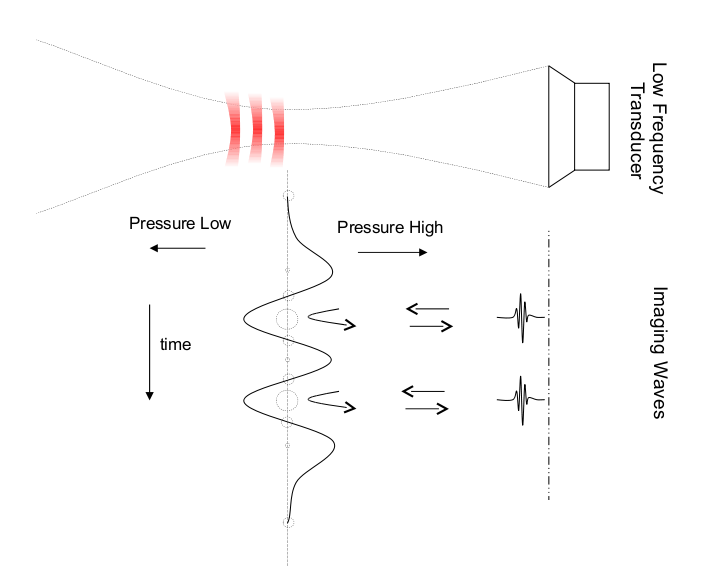
\includegraphics[width=0.8\textwidth]{change_radius.png}
%      \caption{}
% \end{figure}

% \begin{figure}[t]
%      \centering
%           \label{fig:both_waves}
%           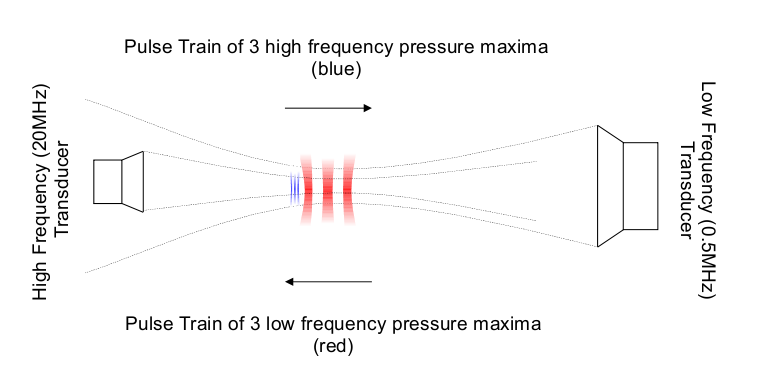
\includegraphics[width=0.8\textwidth]{both_waves.png}
%      \caption{}
% \end{figure}


% Micron-sized bubbles pulsate when insonated at diagnostic frequencies
% and thereby act as acoustic sources that add contrast to ultrasound
% images. They may be functionalised to target specific molecular
% markers but are restricted to the vasculature due to their size, which
% is hard to change. 


% For the microbubbles to  leave the blood through normal capillaries,
% we hypothesise that their size will need to be smaller than about
% 150nm.
% (See, for example, the visiculo-vacuolar transport discussed by
% \cite{Hobbs1998}).
% Tumour vasculature is more leaky with endothelial channels between
% 300-600nm being observed (\cite{Fukumori2006, Hashizume2000,
%   Hobbs1998}),
% although how rare such gaps are within the tumour vasculature is still
% somewhat of an open question (\cite{Hashizume2000}).

% Bubbles much smaller than $\frac{1}{2} \micro\metre$ are hard to manufacture.
% Without a hard stabilising coating such small bubbles dissolve within
% a fraction of a second,
% whereas with a hard shell the bubbles tend to be very stiff.
% Since the resonance frequency of a bubble increases as its radius gets smaller,
% the difficulty in producing small bubbles limits contrast agent  use to the lower resolution frequencies
% (typically below 10MHz).
% Worse still, the  restriction of contrast agents to the blood prevents ultrasound from
% developing into a fully functional imaging modality.

%and for high resolution ultrasound (10-50MHz)
%this requires sub-micron bubbles
%that are difficult to stabilise.
%Indeed, this limitation on how small bubbles can be made restricts
%microbubbles to the blood,
%for bubbles smaller  than 150nm would be required to leave
%the vasculature.

%Clinically there are problems with contrast imaging in ultrasound.
%Micron-sized bubbles seem set to remain the only
%effective method of achieving a high acoustic scattering cross-section in the
%absence of a large acoustic impedance mismatch;
%the scattering mechanism being the re-radiation of sound generated
%by a bubble induced to pulsate by the ultrasound wave,
%as opposed to a difference in the speed of sound across a boundary.
%
%after
%being induced by the ultrasound wave to pulsate
%whereby they are induced to %
%
%Bubbles have proven useful because they rely upon an entirely
%different scattering mechanism.
%They are induced to 
%pulsate by the ultrasound beam and %thereby
%re-radiate the incident sound.
%But microbubble contrast agents have their problems.
%To achieve a large scattering cross-section requires
%the bubbles to pulsate at resonance,
%and for high resolution ultrasound (10-50MHz)
%this requires sub-micron bubbles
%that are difficult to stabilise.
%Indeed, this limitation on how small bubbles can be made restricts
%microbubbles to the blood,
%for bubbles smaller  than 150nm would be required to leave
%the vasculature.

% A brief outline of the general experimental  method used  is given in \secref{Methods}.
% This will give the context not just to the experimental work,
% but also the  theoretical and computational studies.%%

% It is anticipated that there will be significant sound generated from
% when the oil first vapourises into a bubble.
% This is of interest, 
% although is not expected to be very different from previous studies of
% cavitation.
% Of greater interest is the characterisation of the  response of the  induced bubble to the
% high frequency wave.
% The problem is then to study conventional bubble imaging
% in the presence of a low-frequency wave.

% By what mechanism can the low frequency affect how the high frequency
% wave interacts with the bubble?
% There are at least two.
% %Before the study was launched, however,
% %we asked by what mechanisms we expected the low-frequency wave to
% %exert an influence.
% %We believed these to be the main mechanism.
% \desc{
%   \item[Bubble radius:]
%     The resonance frequency of a bubble is a function of
%     the bubble's equilibrium radius.
%     Due to the long wavelength of
%     the low frequency sound, in comparison to the imaging wave,
%     we can imagine it controlling the `ambient pressure' of the
%     bubble when imaged by the high-frequency wave.
%     In this way it will control the equilibrium radius of the bubble,
%     and therefore the bubble's resonance frequency.
%   \item[Bubble wall velocity:]
%     Not only will the low-frequency wave determine the radius of the
%     bubble, but
%     it will also determine the bubble's mean  radial velocity.
%     We therefore expect the bubble to be influenced by a
%     Doppler-shifted imaging frequency.
%     The magnitude of the
%     Doppler-shift will be determined by the low-frequency wave.
% }
%Firstly, the bubble will transiently be of a different radius,
%and so have a different resonance frequency.
%Secondly, the bubble wall will have a velocity and
%so the frequency experienced will be Doppler shifted from the actual
%high-frequency pulse.
%By tuning these  effects, our studies to imaging cavitating
%droplets also has a direct bearing upon high frequency bubble
%imaging.

%We hypothesise that by these effects the scattering of the high-frequency wave 
%will be dependant upon the phase of the low-frequency wave.
%This is important because scattering cross-section of a  bubble may
%then be tuned.
%At certain phases, for example,  the bubble
%will be small and shrinking, and so will have higher natural resonance
%frequency and experience a red-shifted high-frequency wave.
%    This is illustrated in \figref{general_idea}.

% Which of these effects dominate and which parameters matter?
% In what way may we tune the low-frequency wave in order to control the
% scattering of the imaging wave?
% To answer these questions we must turn to the equations that describe how the
% bubble pulsates.
%These are non-linear and so a computational study will be required.

%A further aim of the computational study is to see which of these
%mechanism dominate. 
%Is \surf\ imaging, should it work,  mainly caused by radial
%modulation, or by a Doppler shift?


%There is a problem, however.
%The equations that are commonly used to describe the bubble,
%the Rayleigh-Plesset, Herring-Trilling, Keller-Miksis equations, for
%example,
%do not contain a Doppler effect.
%It is `missing' from the model, 
%even though intuitively it ought to be there.



%  There is a problem, however.
%  The equations that are commonly used to describe the bubble,
%  the Herring-Trilling and Keller-Miksis equations%  Rayleigh-Plesset,
%  , for
%  example,
% % are awkward since their formulation as differential
% % equations, that can be solved only numerically, makes the Doppler-influence hard to study.
% % Indeed, 
% % that there is a Doppler-effect contained within these equations at all
% % is easily missed, 
% % and perhaps this is why the Doppler-contribution to bubble wall motion
% % has not as-of-yet, to the author's knowledge, been studied.


% study differential equations for which 
% have the 
% elation the influence of the Doppler effect.
% The influence is felt in the numerical computation of the equations,
% but it is hard, analytically to delineate it's contribution.

%do not contain a Doppler effect.
%It is `missing' from the model, 
%even though intuitively is ought to be there.
%Furthermore the equations do not `break' when the bubble wall velocity
%exceeds the speed of sound. 

%The Keller-Miksis equation models the radial oscillations of the
%bubble that
%will contribute to the the  far field acoustic wave.
%The validity of the equation at high bubble wall velocities (i.e. near
%the speed of sound, speeds that the bubble wall routinely reach) has been questioned, however
%(\cite{Prosperetti1986}).
%On the one hand, the equation does not break down as it should when the wall
%velocity equals the speed of sound and so it is argued that the
%description when shock waves are present is incorrect.
%On the other hand, however, 
%On the other hand,

%The equations that are commonly used to describe the bubble,
%the Rayleigh-Plesset, Herring-Trilling, Keller-Miksis equations for
%example,
%do not contain a Doppler effect.
%It is `missing' from the model, 
%even though intuitively is ought to be there.
%Furthermore the equations do not `break' when the bubble wall velocity
%exceeds the speed of sound. 

%Since the bubble wall velocity routinely reaches the same order as the speed
%of sound in microbubble physics,
%the resolotuion to this query is required.
%This can be done by deriving the acoustic output of a bubble using the
%older and 
%more general theory of  `aerodynamic' sound.
%This theory was originally  developed in the 1950s to describe the
%acoustic output of jet engines,
%and the general problem of finding the acoustic output of fast moving
%surfaces was solved by \cite{FfowcsWilliams1969}.


%To resolve whether or not the Keller-Miksis equation applies high
%bubble wall velocities, we can compare it with a model especially
%designed for sit the model in a more general setting 
%predictions of , 
%To resolve this, as well as other problems (introduced below), 
%a new equation to describe the bubble wall motion needs to be developed.
%The outline for how this is done is given in \secref{KellerModel}, borrowing heavily from the
%`aerodynamic' theory of sound originally developed in the 1950s to describe the
%acoustic output of jet engines.

%of bubble wall motion that would be used to answer such
%a question (The Rayleigh-Plesset, Herring-Trilling, Keller-Miksis models,
%for example) do not contain a Doppler effect.
%It is missing from the model, even though intuitively, the
%Doppler-effect on the bubble should certainly be there.
%It is missing, however, from the equations generally used to model  bubble wall
%motion (The Rayleigh-Plesset, Herring-Trilling, Keller-Miksis models,
%for example).
%We cannot n


%There is much that can potentially be learned from this dual wave
%approach.

%all the experimental work has been small variations on a common setup.
%To solve the questions raised by these experiments,
%the setup has also influenced the theoretical and particularly
%computational aspects of the project.
%We therefore give an outline first.

%Putting to one side temporally the problem of cavitating the oil,

% A more stable and better understood source of bubbles are those that
% are manufactured commercially for ultrasound imaging.
% We therefore began the experimental work by studying Levovist and Sonovue to
% determine the influence of the low frequency wave on high frequency
% imaging.
% This technique of using a low frequency wave to alter the
% scattering-cross section of a higher frequency wave often goes by the
% name of \surf\ imaging and some experimental results are given
% in \secref{bubble_exp}.

%and is the source of ongoing experimental work.

%As will be seen in \secref{bubble_exp},
%the preliminary  study into \surf\ imaging could not determine a
%strong influence of the low frequency wave.
%To understand why this is, and to try to narrow the viable experimental
%parameters, a computational study was launched.
%The aims of this study were to determine pressures and frequency that
%should be used to obtain the strongest 
%influence of the low frequency wave on the imaging wave.


%\section{Literature Review}


%%% Local Variables: 
%%% mode: latex
%%% TeX-master: "../../tshorrock_thesis"
%%% End: 

\part{Mathematical Introduction}


%%% Local Variables: 
%%% mode: latex
%%% TeX-master: "tshorrock_thesis"
%%% End: 


\chapter{Probability, Inference, and Thermodynamics 50\%}{\label{sec:variationalMethods}

\section{Introduction}

Need a systematic way to make inferences.

This entails using probabilities to model our knowledge of the world.



\section{Probability}



Probability theory studies the consistency of the various statements that can be made of the world.
The statements may or may not be true,
where there is uncertainty in some event, 
each possible outcome results in a valid statement.
%there are many valid statements that can be made of the world, one for each possible outcome.
Statements may be atomic, in that they reference no other event,
or they may be compound, in that they depend upon other, simpler, statements.

Given a set of outcomes to an uncertain event, 
an individual may ascribe each statement with the degree to which it is to be believed.
Probability theory determines how to combine the beliefs of simpler statements
into the belief of their compound in a consistent manner,
and describes how beliefs should change in order to remain consistent when new information becomes available.
Whether the original assignments are based on experience, prejudice or mere caprice,
and whether they coincide with the assignments of any other individual does not matter.
Probability theory concerns itself only with maintaining a self-consistent set of beliefs.
%that depend upon an \apriori\ model that defines the set of possible outcomes.


%The formulation of a set of possible outcomes and the assignment of their beliefs constitutes a model of the uncertain event.
A model first defines the set of possible outcomes and second assigns the \apriori\ beliefs.
It defines  how one interprets the world.
A experimental test can make more precise the parameters of the model,
or one may find that experimental data better supports an alternative model,
but the model is always the starting point.
In this thesis, therefore, an individual's view of the world is characterised by the totality of the models that they use to describe the world.

The subjectivity intrinsic to the possibly capricious formulation of a model may be disconcerting. 
A consistent and agreed upon science can result, however,
when there exists a nature to which differing models may be compared.
Consensus can result by subjecting a model to experimental test and by sharing successful models.

%One last comment is in order, however,
%and that is  the inherent lack of knowledge involved even when carrying out a measurement.
%By this I do not mean the banal problems of finite experimental precision,
%the {\em experimental noise} that introduces uncertainty into the quantity measured.
%Rather, I refer to the difficulties in determining how distances and times are to be measured at all.
%If a signal, such as light or sound, is used to locate a faraway entity
%then the true location of the entity is no longer measurable.
%The experimenter has no knowledge of what happens to that signal after it has been sent and before it returns:
%both the signal's route and speed are unknown.
%Assuming the  signal's route to be direct and speed to be constant throughout is a common and necessary convention, for otherwise no definition of measurement is possible.
%It must, however, be emphasised that in reality the speed of the signal is no more attainable than its path.
%Much more will be said on this matter in \chapref{measurement}.  
%For now we just note that our knowledge of the world, through our models and experiments,
%is, and is set to remain, remote from the true natural order of things.

Before moving on,
the world view adopted by probability theory should be located in its philosophical context.
In this regard the closeness of Wittgenstein's {\em Tractatus Logico-Philosophicus} to modern probability theory should be noted. 
This thesis shall not attempt to unpick where Wittgenstein's views agree and differ from modern probability theory 
(for such an attempt see \cite{WittgensteinLattice}),
and a discussion on the relative merits of other world views is not considered to be within the scope of this thesis.
Nevertheless, %to aid the interested reader in locating the  philosophy of probability theory, 
the reader is invited to keep the following quotes in mind during this chapter.
Firstly, regarding the primacy of models when conceiving the world,  Wittgenstein writes 
\begin{quote}
  The world is the totality of facts, not of things.  For the totality of facts determines both what is the case, and also all that is not the case.  Every thing is, as it were, in a space of possible atomic facts. I can think of this space as empty, but not of the thing without the space. (1.1, 1.12, 2.013)
\end{quote}
Indeed, the facts have a definite structure that is determined by how their compound is formed,
and this structure is assumed to be what is shared with nature:
\begin{quote}
Atomic facts are independent of one another. We make to ourselves pictures of facts. The picture is a model of reality.    
That the elements of the picture are combined with one another in a definite way, represents that the things are so combined with one another.
This connexion of the elements of the picture is called its structure, and the possibility of this structure is called the form of representation of the picture.  (2.061, 2.1, 2.12, 2.15)
\end{quote}
Finally, Wittgenstein expresses very directly the  difficulty in articulating any innate truth that is external to a model of the world:
\begin{quote}
The world and life are one. I am my world. (The microcosm)... [A]t death the world does not alter, but comes to an end. (5.621, 5.63, 6.431)
\end{quote}
The natural world exists, but is  mystical because it can only be guessed at from a constructed world view,
\begin{quote}
Not how the world is, is the mystical, but that it is.  
The contemplation of the world sub specie aeterni is its contemplation as a limited whole. 
The feeling that the world is a limited whole is the mystical feeling. (6.44, 6.45)
\end{quote}
% This thesis shall not attempt to unpick where Wittgenstein views agree and differ from modern probability theory 
% (for such an attempt see \cite{WittgensteinLattice}).
% In the presentation that follows, however,
% propositions from the {\em Tractatus} will periodically be referenced where we believe the viewpoint is the same.
% I hope that this is of interest to the reader.






% and that is the difficulties inherent in carrying out measurements.
% To measure the world, one must decide how to measure the world,
% and in particular, how to measure distances and times.
% Einstein introduced the {\em convension} of using light to carry out measurements.
% However, as is argued in \chapref{measurement},
% other convensions are possible.
% In ultrasound physics, measurements are carried out with and indeed more natural for certain measurements.
% For example 



%  prior to any experiment, 

% Probability theory enables the model to be updated consistently in the light of new experimental evidence,
% and informs us that an experiment agrees with one model better than another.

% An individuals view of the world therefore, 

% In this thesis, therefore, an individual's view of the world is characterised by the totality of the models that they use to describe the world.
% The questions that different individuals puts to the world may be different,
% and so their chosen models will be different too.
% To test the quality of the model, the world must be put to experimental test.
% However, in order to do so, a model is also required for time and space.
% It is impossible to measure beyond these. 



% the degree to which each statement should be believed will often be the subject of disagreement.
% Nevertheless, whether the degrees of belief are 

% The outcome of an uncertain event 
% Individuals may disagree with the likelihood of the various outcomes of an uncertain event.
% Everybody is able to ascribe a degree to which the various outcomes of an uncertain event should be believed.


% but whether based on experience or caprice,
% each can ascribed a degree of belief.
% %but are formed with greater or lesser certainty out of all the possible outcomes to their subject.
% %they are ascribed a degree of belief 
% %A degree of belief, whether based on experience or prejudice, can therefore be ascribed to a statement.


\subsection{The Lattice of Statements}

The compounding of statements can be illustrated in a Hesse diagram.  
This will be illustrated with two examples in this section.
The first is provided by a model for the outcomes for the Shell Game,
where the task is to guess under which cup a ball is placed.
This example is sufficiently simple to guide intuition in the formalism that follows.
The second example is geometric.
This example is useful both because it links to the introduction in geometric probability in \chapref{gc},
but also because it introduces some results of geometric probability that shall be useful later.

\subsubsection{The Shell Game}

\begin{figure}%[htp]
 \centering
\missingfigure{The Shall Game Lattice.}
 \caption{
   A lattice depicting the statements modelling the Shell Game.
}
 \label{fig:ShellGame}
\end{figure}


An example is provided in \figref{ShellGame}, which illustrates a model for the Shell Game.
In this game there are three cups and one ball.
The operator puts the ball under one cup and shuffles them rapidly, 
the player has to follow which cup contains the ball.
(It can be that the game is dishonest, 
and that the ball is removed/placed under a cup by a slight of hand so that the player always looses.
For the time being, however, we focus on the model of a sincere player, 
who enters into the game without considering this dishonesty).

The three independent statements, $\{A,B,C\}$, are that the ball is under cup $A$, $B$ or $C$ respectively.
These atomic statements can be compounded so that $AB$ represents the statement the statement ``The ball is under cup A {\em or} B''.
At the top of the lattice is the statement, $ABC$, which is that the ball is under one of the three cups.
Within the logic of the model, the statement $ABC$ represents certainty.
In reality, of course, it is far from certain that the ball is in fact under one of the cups.
Models do not always reflect reality well.
%but such failures in a model can occur.
The bottom statement, denoted $\absurdity$, is that the ball is under all three cups simultaneously.
This statement is believed to be impossible, and so represents absurdity.

The rules for constructing \figref{ShellGame} should now be clear:
\nlistcompact{
\item Compound statements are constructed from set union.  That is 
  \begin{align}
    AB \equiv A \OR B
  \end{align}
\item Simpler statements are constructed from set inclusion.  Firstly,
  \begin{align}
    \absurdity \equiv A \AND B \AND C.
  \end{align}
  Secondly, the statement $A$ can be recognised as that which is common in from the statements $AB$ and $AC$,
  \begin{align}
    A \equiv AB \AND AC.
  \end{align}
}
It follows that the ordering of statements obeys an algebra (the algebra of sets),
from which it follows that the diagram of \figref{ShellGame} forms a lattice.

% \subsubsection{Geometric subspaces}

% \begin{figure}%[htp]
%  \centering
% \missingfigure{The Geometric Subspace Lattice.}
%  \caption{
%    A lattice depicting the subspaces in three dimensional Euclidean geometry
% }
%  \label{fig:Lattice_3D_sub}
% \end{figure}
% A second and more physical example of a lattice of statements is provided from geometry.

\subsection{Fundamental Symmetries of Probability Theory}
Must ascribe scalar quantification.


Knuth and Skilling\cite{Knuth2010} recently introduced a set of  minimal symmetries that are required for statements in probability theory.


\subsection{Measure}


The first of these are 
\nlist{
  \item Null element:
    \begin{align}
      \absurdity \OR x = x
    \end{align}
  \item 
    Ordering of Join
    \begin{align}
      x \le x \OR y
    \end{align}
    for non-null $y$.
  \item
    Join preserves order from right or left
    \begin{align}
      x \le y \implies \left\{
        \begin{array}{l}
          x \OR z \le y \OR z\\
          z \OR x \le z \OR y
        \end{array}
      \right.
    \end{align}
  \item 
    Join assumed to be associative 
    \begin{align}
      \lr{x \OR y} \OR z = x \OR \lr{y \OR z}
    \end{align}
}
By making reference to the Shell Game, 
these symmetries define properties that would be expected for statements.
For instance, if the proposition that the ball is everywhere is deemed by the model to be absurd, 
then the statement that the ball could be everywhere or under cup $C$ should certainly reduce to
the view that the ball is under cup $C$.


Comment on geometrical interpretation.

\subsubsection{Quantification}
The statements may be quantified.  
A scalar valued quantification may be given to the statement, $x$, 
and will be denoted $m(x)$.

Set the convention that $\absurdity = 0$
so that axiom 1 becomes:
\begin{align}
  0 \oplus x = x
\end{align}



\subsection{Divergence}


\section{Thermodynamics}

Jaynes approach to thermodynamics goes here.

\subsection{Thermodynamic quantities}


\subsection{Old Stuff}

Probability distributions can be used to represent our knowledge of the world.
For example, the value of a  experimentally obtained variable will in general
fluctuate around its average.  
If different runs of the experiment are independent
then the  distribution of obtained values fully describes the experiment.

What is learned from a given experiment is then characterised with how the probability distributions
that represent our knowledge change.
If a hypothesis, $\H$, is that a set of experimental data, $\vx = \{x_n|n=1,\ldots,N\}$, should conform to a model with a set of parameters, $\vw = \{w_i| i=1,\ldots,I\}$,
then our full knowledge of the system is given by the joint probability distribution
\begin{align}
  P\lr{\vx,\vw,\H}.
  \label{eqn:fullJointDist}
\end{align}
Of greater importance than \eqnref{fullJointDist}, however,
is to determine how our knowledge of the model changes when we collect the experimental data.
This can be found from  \eqnref{fullJointDist} by splitting the joint distribution into its conditional probabilities.
\begin{align}
  P\lr{\vx,\vw,\H} = P\lr{\vw|\vx,\H}P\lr{\vx|\H}
  =  P\lr{\vx|\vw,\H} P\lr{\vw|\H}.
\end{align}
from which it follows that 
\begin{align}
   P\lr{\vw|\vx,\H} =  \frac{P\lr{\vw|\vw,\H} P\lr{\vw|\H}}{P\lr{\vx|\H}}.
  \label{eqn:BayesTheorem}
\end{align}
Equation \Eqnref{BayesTheorem} is Bayes Theorem.
It states that the probability of the model's parameters, {\em given the data},
can be determined from the probability of the data when the parameters are known, and the a  probability of parameters {\em before the data was known}.
It describes exactly the process of inference.

The term $P\lr{\vx|\vw,\H}$ is the likelihood function.
It evaluates the degree to which the model with a given set of parameters agrees with the experimental data.
If it is assumed that every data point is independent, and that each datum should agree with the prediction of the model, $t_n$, 
to within Gaussian noise
then the likelihood function would be,
\begin{align}
  P\lr{\vx|\vw,\H} = \prod_{n=1}^N \sqrt{\frac{\gamma}{2\pi}}e^{-0.5\gamma\lr{x_n-t_n}^2}.
\end{align}
The variable $\gamma$ is the precision - the inverse of the variance - and is one of the set $\{w_i\}$.

The term $P\lr{\vw|\H}$ in \eqnref{BayesTheorem} is independent of the experimental data $\{x_n\}$.  
It  represents our knowledge of the parameters before the experiment was carried out.
It could be that the parameters are already known to great precision - 
in which case the probability distribution would tend towards a delta function.
Alternatively, it could that the a priori knowledge of the precision, say, 
does not expend beyond the requirement that the precision is positive definite.
In this case the prior distribution would be represented by a scale invariant positive definite distribution.
One such example is the Gamma distribution,
\begin{align}
  P(\gamma|s,c) = \frac{1}{\Gamma(s)c}\lr{\frac{x}{s}}^{c-1}\exp\lr{-\frac{x}{s}},
\label{eqn:Gamma}
\end{align}
in the limit such that $sc = 1$ and $c\rightarrow 0$ \cite{MacKay2003}.

The hypothesis, $\H$,  encompasses all of the assumptions that go into the inference.
These include the choice of the model that is fitted to the data, 
the prior probabilities assigned to the model variables and the 
the noise model described by the likelihood function.
These assumptions are inevitable - they reflect our uncertainty 
 prompts the experiment in the first place.
However, 
since many different hypotheses can be dreamed up,
it is important to be able to be able to evaluate how each is supported by the experimental data.
For this, Bayes Theorem can be applied a second time:
the probability of the hypothesis, given the data, is
\begin{align}
P\lr{\H | \vx } = \frac{P\lr{\vx|H}P\lr{\H}}{P\lr{\vx}}.
\label{eqn:BayesHyp}
\end{align}
Since the probability of the data, $P\lr{\vx}$, 
is independent of the hypothesis
it can be eliminated when comparing two hypotheses, $\H_1$ and $\H_2$,
\begin{align}
\frac{P\lr{\H_1 | \vx }}{P\lr{\H_2 | \vx }} = \frac{P\lr{\vx|\H_1}}{P\lr{\vx|\H_1}}\frac{P\lr{\H_2}}{P\lr{\H_2}}.
\label{eqn:ModelCmp}
\end{align}
The second of the ratios on the right-hand-side of \eqnref{ModelCmp}
give an opportunity, if desired, to prefer one model over another irrespectively of any data collected.
The first quotient is determined from the experimental data.
The term $P\lr{\vx|\H}$ is called the evidence and it is the partition function of  \eqnref{BayesHyp}.

A model that is highly constrained will be inflexible in the range of predictions it can make,
whereas a model that has many free parameters will be able to predict a vast number of possible outcomes.
The more constrained model will therefore have a smaller set of likely outcomes,
but each of these will have a much greater probability than the many possible outcomes of the less constrained model.
The right-hand-side of \eqnref{ModelCmp} therefore directly and quantitively embodies Occan's razor,
the rule of thumb that states that `simpler' models should be favoured over more complicated models.
For a more detailed discussion of model comparison and Occan's razor see \cite[Chapter 28]{Mackay2003}.

To evaluate the evidence the numerator in equation \eqnref{BayesTheorem} must be integrated over the entire parameter space,
\begin{align}
  P\lr{\vx|\H} = \int_\vw d\vw P\lr{\vw|\vw,\H} P\lr{\vw|\H}
\end{align}
In general this cannot be done analytically.
However, it is often the case that the probability density tightly peaked about the maximum.
In this case the evidence may be evaluated by approximating the peak with a Gaussian, which can be integrated.
This is the saddle point approximation.
Expanding the logarithm of the  unnormalised probability distribution, $P^\ast$, 
around the maximum, $\vx_0$,
gives
\eq{
  \ln P^\ast = \ln P^\ast(\vx_0) - \frac{1}{2}\lr{\vx-\vx_0}^T \vA\lr{\vx-\vx_0 }
}
where 
\eq{
\vA = A_{ij} = \frac{\d^2}{\d x_i\d x_j} \ln P^\ast(\vx_0)
}
is the Hessian matrix.
The right-hand-side of equation \eqnref{BayesTheorem}  is therefore approximated by the multidimensional Gaussian
\begin{align}
   P\lr{\vw|\vx,\H} = P^\ast(\vx_0) \exp \lr{- \frac{1}{2}\lr{\vx-\vx_0}^T \vA\lr{\vx-\vx_0 }}
\end{align}
for which the normalisation constant, the evidence, is 
\begin{align}
   P^\ast(\vx_0) \sqrt{\frac{\lr{2\pi}^K}{\det \vA}}
\end{align}


\subsection{Conjugate Exponential Variables}
\begin{align}
\ln P(X|Y) = \phi(Y) u(X) + f(X) + g(Y)
\end{align}
then conjugacy implies
\begin{align}
\ln P(W|X) = \tilde\phi(W) u(X) + h(W).
\end{align}
so that variable $X$ is treated the same.

\section{Variational Approach}

\section{Kullback-Leibler divergence}

Variational methods can be used to approximate a probability distribution, $P$, that is impossible to evaluate exactly, 
with a probability distribution that is more maluable.
The approximation is varied so that it matches the original distribution as closely as possible. 


The amount of information that is lost when a distribution $Q$ is used in place of the distribution $P$ is measured by the relative entropy, 
a quantity known as the  Kullback-Leibler divergence.
%The Kullback Leibler divergence gives a measure of the similarity of two distributions,
It is defined,
\begin{align}
\KLD{Q}{P} &= \int_\vH Q(\vH|\H) \log\frac{Q(\vH|\H)}{P(\vH|\vD,\H)} d\vH,
\end{align}
where $P$ and $Q$ are probability distributions that model a hypothesis, $\H$.
$\vH$ is a set of unknown variables that form the model and $\vD$ is as set of known variables.
From Gibbs inequality it follows that 
\begin{align}
\KLD{Q}{P} \ge 0
\end{align}
and equality is only when $P=Q$.
That is, knowledge of the system is always lost when it is approximated.

The Kullback-Leibler divergence will be minimised in two different ways in this thesis.

\section{Statistical Mechanics}

  Let 
  \begin{align}
    P = \frac{1}{Z} e^{-\beta \scalar{E} }
  \end{align}
  then
  \begin{align}
    \beta \tilde{F} &= \int Q(x) \ln \frac{Q(x)}{\exp\lr{-\beta \scalar{E} }} \\
    &= \int Q(x) \ln \frac{Q(x)}{P} - \ln Z \\
    &= \KLD{Q}{P} - \ln Z
    &= \KLD{Q}{P} + F.
  \end{align}
  where $F \equiv  - \ln Z$ is the free energy and 
  \begin{align}
    Z = 
  \end{align}

\section{Variational Ensemble Learning}


This property makes the Kullback-Leibler divergence a useful function minimise.
Indeed, using $P(\vH,\vD|\H) = P(\vH|\vD,\H) P(\vD|\H)$, 
we may write,
\begin{align}
  \KLD{Q}{P}  % &=\int_\vH Q(\vH) \log\frac{Q(\vH)}{P(\vH|\vD)} d\vH \\
  &= \int_\vH Q(\vH|\H) \log\frac{Q(\vH|\H)}{P(\vH,\vD|\H)} d\vH  +  \log P(\vD|\H) \\
  &= -S_Q - \int_\vH Q(\vH|\H) \log P(\vH,\vD|\H)  d\vH + \log P(\vD|\H)
\end{align}
where $S_Q = - \int_\vH Q(\vH|\H) \log Q(\vH|\H) d\vH$ is the entropy given the hypothesis%
\footnote{
\begin{quote}
Consider, for example, a crystal of Rochelle salt.
For one set of experiments on it, we work with temperature, pressure and volume.
The entropy can therefore be expressed as some function $S_e(T,P)$.
For another set of experiments on the same crystal,
we work with temperature, the component $e_{xy}$ of the strain tensor,
and the component $P_z$ of the electric polarisation;
the entropy as found in these experiments is a function $S_e(T, e_{xy}, P_z)$.
It is clearly meaningless to ask ``What is the entropy of the crystal?''
unless we first specify the set of parameters which define its thermodynamic state.%

One might reply that in each of the experiments cited, 
we have used only part of the degrees of freedom of the system,
and there is a ``true'' entropy which is a function of all these parameters simultaneously.
However we can always introduce as many parameters as we please...
There is no end to this search for the ultimate ``true'' entropy until we have reached the point where we control
the location of each atom independently.
But just at that point the notion of entropy collapses, and we are no longer talking thermodynamics!

From this we see that entropy is an anthropomorphic concept,
not only in the well known statistical sense that it measures the extent of human ignorance as to the microstate.
{\em Even at the purely phenomenological level, entropy is an anthropomorphic concept.}
For it is a property, not of the physical system,
but of the particular experiments that you or I choose to perform on it.

\flushright Edwin T. Jaynes\cite{Jaynes1965}
\end{quote}
}.
Define the  cost function
\begin{align}
  \L =  \int_\vH Q(\vH) \log P(\vH,\vD) ) d\vH +S_Q  
\end{align}
From which it follows that
\begin{align}
  \L &=   \log P(\vD,\H) - \KLD{Q}{P} \\
     &\le \log P(\vD,\H)
\end{align}
The probability of the model is 
\begin{align}
  P(\H, \vD) &=    \frac{P(\vD, \H) P(\H)}{P(\vD)}\\
             &\le  \frac{\L(Q)P(\H)}{P(\vD)}
\end{align}
Assuming that the variables are independent gives
\begin{align}
Q\lr{\vH} = \prod_n^N Q_n\lr{H_n}
\end{align}
where $Q_n$ is the independent distribution for the $n$th variable.
Then 
\begin{align}
  \L&=  \int_\vH \prod_n^NQ_n(H_n) \log P(\vH,\vD) ) d\vH - \sum_n^N \int_\vH Q_n(H_n)  \log Q_n(H_n|\H) dH_n
\end{align}
Separating out the $j$th element gives
\begin{align}
  \L &= \int_\vH Q_j(H_j)\prod_{n\ne J}^NQ_n(H_n) \log P(\vH,\vD) ) d\vH + S_{Q_j} +  \sum_{n\ne j}^N S_{Q_{n}}
   \\ &= \int_{H_j} Q_j(H_j) \multi{\log P(\vH,\vD)}{\prod_{i\ne j} Q_i\lr{H_i}} +S_{Q_j} +  \sum_{n\ne j}^N S_{Q_{n}}
\end{align}
Introducing
\begin{align}
  Q^\ast_j = \frac{1}{Z}e^{\multi{\log P(\vH,\vD)}{\prod_{i\ne j} Q_i{H_i}}}
\end{align}
gives
\begin{align}
\L &= \int_{H_j} Q_j(H_j) \log Q^\ast dH_j  +S_{Q_j} +  \sum_{n\ne j}^N S_{Q_{n}} - \log Z
\\ &= \KLD{Q_j}{Q^\ast_j}  - \log Z -  \sum_{n\ne j}^N S_{Q_{n}} 
\end{align}
which is maximal with respect to $Q_j$ when $Q_j = Q^\ast_j$, and so the function is maximised when
\begin{align}
  \log Q^\ast = \multi{\log P(\vH,\vD)}{\prod_{i\ne j} Q_i\lr{H_i}}
\end{align}
 
Now 
\begin{align}
  P(X_1, X_2, \ldots, X_N) = \prod_i^N P(X_i|\parents{i})
\end{align}
 so 
 \begin{align}
 \ln Q^\ast_j(H_j) = \multi{\ln P\lr{H_j|\parents{j}} + \sum_{i \in  \children{j}} \ln P\lr{X_i| H_j, \coparents{j}}}{\sim Q(H_j)} + \const
 \end{align}
If conjugate exponential models then
\begin{align}
\ln Q^\ast_j(H_j) &= \multi{\phi(\parents{j}) u(H_j) + f(H_j) + g(\parents{j}) }{\sim Q(H_j)}
\nonumber \\
&+\multi{\sum_{i \in  \children{j}}  \tilde\phi(X_i,\coparents{j}) u(H_j) + h(X_i,\coparents{j})  }{\sim Q(H_j)} + \const\\
&= \multi{\phi(\parents{j}) + \sum_{i \in  \children{j}}  \tilde\phi(X_i,\coparents{j}) }{\sim Q(H_j)} u(H_j)+ f(H_j)+\const
\end{align}
from which it follows that
\begin{align}
  \phi^\ast_j = \scalar{\phi(\parents{j})} + \sum_{i \in  \children{j}}  \scalar{\tilde\phi(X_i,\coparents{j}) }
\end{align}
where expectations are with respect to $Q$.

The message from a variable node to a function node is
\begin{align}
  m_{X_i\rightarrow f_j} = \Moments{Q_i}
\end{align}

The message from a function node to a variable node is
\begin{align}
  m_{f_i\rightarrow X_j} = \Natural{\multi{f_i(\neighbour{i})}{Q_{{\neighbour{i} \bs X_j}}}}
\end{align}
Updated variable node is then given by
\begin{align}
  \Natural{Q^\ast(X_i)} = \sum_{j\in\neighbour{i}} m_{f_j \rightarrow X_i}
\end{align}







\section{Independent Components of the pulses}

Assume differing bubble sources as independent components in bubble.

\begin{align}
\vx_t = \vA \vs_t
\end{align}
One model for this is a Gaussian
\begin{align}
  P(x_t| \Lambda) = \G(x_t; AS_t, \Lambda)
\end{align}
However,
from the \figref{} it is seen that the Gaussian noise model is not good.
A better alternative is to use Fourier decomposition,

\begin{align}
  \vx_\omega = \vA \vs_\omega
\end{align}
such that
\begin{align}
  P(\vx_\omega| \Lambda_\omega) = \G( \vx_\omega ; AS_\omega, \Lambda_\omega)
\end{align}

\begin{align}
  P(\vH|\vD) = G(\vH)
\end{align}
\begin{align}
\KLD{Q}{P} &= \int_\vH Q(\vH) \log\frac{Q(\vH)}{P(\vH|\vD)} d\vH \\
  &= \int_\vH Q(\vH) \log\frac{Q(\vH)}{P(\vH,\vD)} d\vH  + \int_\vH Q(\vH) \log P(\vD) d\vH\\
  &= \int_\vH Q(\vH) \log Q(\vH) d\vH - \int_\vH Q(\vH) \log Q(\vH) \log P(\vH,\vD) ) d\vH + \log P(\vD)
\end{align}
Bring cost function
\begin{align}
  \L =  \int_\vH Q(\vH) \log Q(\vH) \log P(\vH,\vD) ) d\vH - Q(\vH) \log Q(\vH) d\vH 
\end{align}
From which it follows that
\begin{align}
  \L &=   \log P(\vD,\H) - \KLD{Q}{P} \\
     &\le \log P(\vD,\H)
\end{align}
The probability of the model is 
\begin{align}
  P(\H, \vD) &=    \frac{P(\vD, \H) P(\H)}{P(\vD)}
             &\le  \frac{\L(Q)P(\H)}{P(\vD)}
\end{align}


\subsubsection{The model}
\begin{align}
  P(s_{m\omega}| \H) &= \sum_{c=1}^{N_c} \pi_{mc}\G(s_{m\omega};0,\beta_{\omega c})\\
  P(\beta_{\omega c} &= \GammaDistr(\beta_{mc} ; b^{(\beta)}, c^{(\beta)})\\
  P(\{\pi_{mc}\}_{c=1}^{N_c}|\H)  &= \Dirichlet\lr{ \{\pi_{mc}\}_{c=1}^{N_c} | c^{(\pi)}}
\end{align}
And mixture
\begin{align}
  P(A_{nm}|\H) &= \G(A_{nm}; 0,\alpha_m)\\
  P(\alpha_m| \H) &= \GammaDistr(\alpha_m| b^{(\alpha)},c^{(alpha)})
\end{align}
and gamma
\begin{align}
  P(\Lambda_{\omega},\H) = \GammaDistr(\Lambda_\omega;b^{(\Lambda)},c^{(\Lambda)} )
\end{align}

Simplify the distribution
\begin{align}
Q\lr{\vs, \vA, \pi, \beta, \alpha, \Lambda} = Q\lr{s_{\omega m}}Q\lr{A_{nm}}Q\lr{\pi}Q\lr{\beta}Q\lr{\alpha}Q\lr{\Lambda}
\end{align}

\begin{align}
  Q\lr{s_{nm}} = \G(s_{m \omega};\hat{s}_{m\omega}, \tilde{s}_{m\omega})\\
  Q\lr{A_{nm}} = \G(A_{mn};\hat{A}_{mn}, \tilde{A}_{mn})\\
  Q\lr{\beta_{mc}} = \Gamma(\beta_{mc};\hat{A}_{mn}, \tilde{A}_{mn})
\end{align}




\section{Density Functional Theory}\label{app:DFT}


\subsection{Introduction, General Thermodynamics}

\Dft\ relaxes the capillary approximation used in \cnt.
The density of the nucleated bubble is not assumed to be that of the bulk,
and the interface is not assumed to be macroscopic and plainer\cite{Oxtoby1992, Oxtoby1998}.
\Dft\ therefore does a much better job at modelling the interface than \cnt.
Rather than it being a sudden boundary,
there is a finite interval over which the density varies from that of the fluid to that of the vapour
and the bubble is modelled for what it is -  a fluctuation in density - 
rather than a vapour entrapped in  flexible boundary.

If  spherical symmetry is assumed then 
the bubble boundary is defined by its radius.
The critical radius is such that\cite{Oxtoby1992,Oxtoby1998}
\begin{align}
  \frac{d \Omega}{d a} =0,\quad\text{at $a = \astar$} \label{eqn:DFT:astarR}
\end{align}
where $\Omega$ is the {\em grand potential}.


The grand potential in \eqnref{DFT:astar} is difficult to evaluate, however,
as it is a functional of the 
phase space positions of all $N$ molecules in the system.
Specifically,  
\begin{align}
  \Omega = -\beta^{-1}\ln \Xi.
\end{align}
where $\Xi$ is the grand partition function
\begin{align}
  \Xi = \Tr \exp\lr{-\beta \lr{\H - \mu N}}. \label{eqn:nuc:GPF}
\end{align}
 $\Tr$ denotes the trace operator
\begin{align}
  \Tr \equiv \sum_{N=0}^\infty \frac{1}{h^{3N}N!} \iint d\cx_1 d\cp_1
\end{align}
and we have compacted the integral by writing 
\begin{align}
d\cx_n &\equiv dr_n dr_{n+1}\ldots dr_N, &&\quad\text{and}&
d\cp_n &\equiv  dp_n dp_{n+1}\ldots dp_N.
\label{eqn:dshorthand}
\end{align}
In \eqnref{nuc:GPF} $\mu$ denotes the chemical potential and $\H$ denotes the Hamiltonian of the molecules.

The difficulty in evaluating $\Omega$ comes from the interactions between the  molecules.
In order to consider the couplings explicitly we split $\H$ into 
\sub{
\begin{align}
%  \begin{array}{ll}
  \KE &= \sum_i^N \frac{p_i^2}{2m}, && \text{which is the kinetic energy,}\label{eqn:nuc:Kinetic}\\
  \UE &= \UE(\cx_1), && \text{the internal energy and}\\
  \VE &= \sum_i^N V_\ext(r_i) && \text{the external potential.}
%  \end{array}
\end{align}
}
so that the overall Hamiltonian can be written %in terms of the intrinsic potentials, $\H_\in$ and external potential, $\H_\ext$,
\begin{align}
  \H =  %\H_\in + \H_\ext = 
\KE + \UE + \VE.
\end{align}
Here were have extended the shorthand  employed in  \eqnref{dshorthand} so that 
\begin{align}
\cx_n \equiv r_n,r_{n+1},\ldots,r_N,  \quad\text{and}\quad
\cp_n \equiv  p_n,p_{n+1},\ldots, p_N.
\end{align}
By noting that $\KE$ is a function only of momentum, 
and that $\UE$ and $\VE$ are a function only of position, 
the integrals may be split into the respective kinetic and potential partition functions, $Z_\KE$ and $Z_{\UE+\VE}$,
\begin{align}
  \Xi &=     \sum_{N=0}^\infty\frac{1}{N!}  \int d \cp_1  \frac{1}{h^{3N}} e^{-\beta \lr{\sum_i^N \frac{p_i^2}{2m}-\mu N}}  \int d\cx_1 e^{-\beta(\UE +\VE)} \\ 
      &\equiv \sum_{N=0}^\infty\frac{1}{N!} Z_\KE Z_{\UE+\VE}\label{eqn:XiSeparate}
\end{align}
%The coupled terms are therefore the internal energy,  $\UE$.
%Separating the Hamiltonian in this way lets us split the grand partition function
%\begin{align}
%  \Xi = \Tr e^{-\beta (\KE -\mu N)}e^{-\beta(\UE +\VE)}=  \frac{1}{N!}Z_\KE Z_{\UE+\VE}, \label{eqn:XiSeparate}
%\end{align}
%with the second equality following because $\KE$ is a function of only the particle momentums,
%and $\UE$ and $\VE$ are functions of positions.
%At equilibrium the joint probability density of the distribution is the Boltzmann distribution 
%\begin{align}
%  p_0(\cx_1, \cp_1) = \Xi^{-1} \exp\lr{-\beta \lr{H_N - \mu N}}.
%\end{align}
%which can be derived with the Maximum entropy principle\cite{}, for example.
%Here were have extended our shorthand  of \eqnref{dshorthand} so that 
%\begin{align}
%\cx_n \equiv r_n,r_{n+1},\ldots,r_N,  \quad\text{and}\quad
%\cp_n \equiv  p_n,p_{n+1},\ldots, p_N.
%\end{align}
The two functionals, $Z_\KE$ and $Z_{\UE+\VE}$, can be considered separately:
\nlist{
\item The momentum integrals in \eqnref{XiSeparate} form the partition function of an ideal gas,
with 
\begin{align}
  Z_\KE = \int d \cp_1 e^{-\beta \lr{\sum_i^N \frac{p_i^2}{2m}-\mu N}} = \lr{\frac{m}{2\pi\hbar^2 \beta}}^{3N/2} \equiv n_Q^N.
\end{align}
The term $n_Q$ is sometimes known as the {\em quantum concentration} and is related to the {\em thermal de Broglie wavelength}, $\lambda_T$ by $n_Q = 1/\lambda_T$.
We demote the derivation of this standard result  to \appref{DFT}.
\item
  To make progress with the term $Z_{\UE+\VE}$,
% is the  partition function to the joint probability distribution of the  molecular positions,
% %
%
% \begin{align}
%    p_0(\cx) = \frac{1}{N!Z_{\UE+\VE} } e^{-\beta\lr{\UE+\VE}}
%  \end{align}
%  To make progress  
we must  approximate the coupled interaction term, $\UE$.
%so that \eqnref{XiSeparate} can be solved.
Here we assume that only the two particle interactions are important
and write
\begin{align}
  \UE(\cx) \approx \Phi(\cx) =  \sum_{j>i} \sum_i^N \phi(\vr_i, \vr_j),
\end{align}
where $\phi(\vr_i, \vr_j)$ is the two particle potential between a particle at $r_i$ and $r_j$.
%At equilibrium the true joint probability density is the Boltzmann distribution 
%\begin{align}
%  p_0(\cx_1, \cp_1) &= \Xi^{-1} \exp\lr{-\beta \lr{\H_N - \mu N}} 
%\end{align}
%
The approximate Hamiltonian is then $H \equiv \KE + \Phi + \VE$,
and is described by the approximate  probability density, $p$,
  \begin{align}
    p(\cx) = \frac{1}{N!Z_{\UE+\VE} } e^{-\beta\sum_{j>i} \sum_i^N \phi(\vr_i, \vr_j) -\beta\sum_i^N V_\ext(\vr_i)} \label{eqn:pspatial}
  \end{align}
  Marginalising equation \eqnref{pspatial} for the  1-particle distribution gives
  \begin{align}
    p^{(1)}(\vr_1) = \frac{N}{N! Z_{\UE+\VE}} \int e^{-\beta\sum_i^N V_\ext(\vr_i)} d\cx_2. \label{eqn:ponespatial}
  \end{align}
  The 2-particle density is 
  \begin{align}
    p^{(2)}(\vr_1, \vr_2) = \frac{N(N-1)}{N!Z_{\UE+\VE}}\int e^{-\beta\sum_{j>i} \sum_i^N \phi(\vr_i, \vr_j)-\beta\sum_i^N V_\ext(\vr_i)} d\cx_3.
  \end{align}
  The approximate number density, $\rho(\vr)$, is a such that
  \begin{align}
    \int \rho_0(\vr) d\vr = N .
  \end{align}
  It follows that
  \begin{align}
    \rho(\vr) = N!  p^{(1)}(\vr_1). \label{eqn:rhoone}
  \end{align}
  From \eqnref{rhoone} and \eqnref{ponespatial} we find that the {\em density is functional of the external potential.}
}

 The converse is also true:
 {\em the external potential is uniquely determined by the density},
 a result known as the Hohenberg-Kohn theorem.
 The probability density is then determined by the external potential,
 from which it follows that the probability density is a unique functional of the density.
 We outline a proof of the Hohenberg-Kohn theorem in \appref{Hohenberg_Kohn}.
 

It is thereby permissible to work with the mass density rather than the probability density when considering the thermodynamics of the bubble.
Since the density is the term of interest bubble nucleation, the density functional approach is much more direct.



%Re-expressing the grand potential as a functional of mass density rather than probability density
%does not get us any closer to being able to evaluate $\Omega$, however.
%So far the argument is standard from statistical physics.
%To make progress  we must  approximate the coupled interaction term, $\UE$.
%so that \eqnref{XiSeparate} can be solved.
%Here we assume that only the two particle interactions are important
%and write
%\begin{align}
%%  \UE(\cx) \approx \Phi(\cx) =  \sum_{j>i} \sum_i^N \phi(\vr_i, \vr_j),
%\end{align}
%where $\phi(\vr_i, \vr_j)$ is the two particle potential between a particle at $r_i$ and $r_j$.
%At equilibrium the true joint probability density is the Boltzmann distribution 
%\begin{align}
%  p_0(\cx_1, \cp_1) &= \Xi^{-1} \exp\lr{-\beta \lr{\H_N - \mu N}} 
%\end{align}
%
%The approximate Hamiltonian is then $H \equiv \KE + \Phi + \VE$,
%and is described by the approximate  probability density, $p$.
The approximate density function is $\rho$, which defines an approximate grand potential $\Omega_V\lrs{\rho}$.
The task is then to find the distribution $\rho$ that comes closest to approximating $\rho_0$.

The {\em relative entropy } or {\em Kullback-Leibler divergance} gives the amount of information lost 
when using the approximate distribution  $p$ rather than the correct distribution $p_0$,
and is defined
\begin{align}
  \KLD{p}{p_0} = \Tr p \log \frac{p}{p_0} \label{eqn:nuc:KLD}
\end{align}
$\KLD{p}{p_0} \ge 0$, which follows from Gibbs inequality, and only if $p=p_0$ does $\KLD{p}{p_0} = 0$.
We may therefore define
\begin{align}
 \Omega_V\lrs{\rho} \equiv \beta^{-1}\KLD{p}{p_0}+   \Omega\lrs{\rho_0}, 
\end{align}
The approximate  grand potential approaches the true value when 
it vanishes  with respect to $\rho$.
 $\Omega_V\lrs{\rho} $ will then be at thermodynamic equilibrium
which occurs at the critical radius.
Therefore,
condition \eqnref{}
may be expressed\cite{Oxtoby1992}
\begin{align}
  \frac{\delta \Omega_V}{\delta \rho} =0,\quad\text{at $\rho = \rhostar$.} \label{eqn:DFT:astar}
\end{align}

More generally, from \eqnref{} we have
\begin{align}
  \Omega_V\lrs{p} &= \beta^{-1} \Tr p \log \frac{p}{p_0}  - \beta^{-1}\ln \Xi \\
  &= \beta^{-1} \Tr p \log \frac{p}{e^{-\beta\lr{\H - \mu N}}}\\
%  &= T S +    \Tr p \lr{H_N - \mu N} \\
  &= - T S_p + \H_p - \mu N_p \\
  &= F_p - \mu N_p\\
 &= \F + \int V_\ext d\rho - \int \mu d \rho.
\end{align}
where the subscript $p$ indicates an average with respect to the distribution $p$ so that  $S_p$ is the entropy with respect to $p$,
\begin{align}
 \F\lrs {\rho_0} = \Tr p \log\frac{p}{e^{-\beta H_\in}} = \KE + \Phi - TS_p
\end{align}
and the labels `$\in$' and `$ext$' indicates the intrinsic and external parts of the  Hamiltonian.

The energy $\Phi$ at when  $\rho = \rhostar$ (thermodynamic equilibrium)
may be evaluated from by minimising $\Phi\lrs{\phi}$,
\begin{align}
\frac{\delta \Phi}{\delta \phi(r_i, r_j) } &= - \beta^{-1} \frac{\delta \ln Z_{\Phi+\VE}}{\delta \phi(r_i, r_j)} \\
&= \frac{N(N-1)}{2 Z_{\Phi+\VE}}\int d\cx_1 \phi(\vr_1,\vr_2) e^{-\beta\sum_{j>i} \sum_i^N \phi(\vr_i, \vr_j)-\beta\sum_i^N V_\ext(\vr_i)} \\
&= \half \iint d\vr_1 \dr_2 \phi p^{(2)}(\vr_1,\vr_2)
\end{align}
%\begin{align}
%  &= \frac{1}{N!}\frac{e^{-\beta (\KE -\mu N)}}{Z_\KE}\frac{e^{-\beta(\UE +\VE)}}{Z_{\UE+\VE}}  \label{eqn:Jointpzero} %\equiv p_\KE p_{\lr{\UE + VE}}
%\end{align}


%and introduce radial distribution function
%\begin{align}
%  g(r_{12}) = \frac{V^2}{N^2} P_2(r_1, r_2)
%\end{align}


%Since $\UE$ is a measured quantity, it is averaged equilibrium joint probability distribution, $p_0$,
%where $p_0$ is a Boltzmann distribution,
%\begin{align}
% p_0(\cx_1, \cp_1) = \Xi^{-1} \exp\lr{-\beta \lr{H_N - \mu N}}. \label{nuc:pzero}
%\end{align}
%Decoupling the interactions in $\H$ implies that the approximate Hamiltonian, $H$, is described by some likewise decoupled approximate probability distribution, $p$.
%The task is then to vary $p$ so that it matches $p_0$ as closely as possible. %, given its new structure, so that $H$ approaches $\H$.
%From \eqnref{nuc:pzero} $p_0$ is explicitly a function of $\V$.


% This is the 
%  When considering the thermodynamics of the bubble

% The density functional approach is entirely analogous to this next step  but works directly with an approximate mass density, $\rho$, rather than the approximate probability density, $p$.
% The mass density is then varied directly to find the functional form that best matches the equilibrium density, $\rho_0$, and whence the equilibrium Hamiltonian, $\H$.
% Since the density is the term of interest bubble nucleation, the density functional approach is much more direct.
% \Dft\ works at all because
% \nlist{
%   \item 
%     The mass density is a functional of the probability density, $\rho = \rho[p]$.
%     This follows almost trivially from the fact that the equilibrium density is a measured quantity,
%     and therefore an average over $p_0$.
%     Denoting the average
%     \begin{align}
%       \rho\lrs{p} =  \scalar{\rho(\cx_1, \cp_1) }_{p} \equiv \Tr p(\cx_1, \cp_1) \rho(\cx_1, \cp_1), 
%     \end{align}
%     we find that $\rho\lrs{p_0} = \scalar{\rho(\cx_1, \cp_1) }_{p_0}  = \rho_0$.

%     Since the density is a functional of $p_0$, which is in turn a function of $\VE$,
%     it follows that the {\em density is functional of the external potential.}
%   \item
%     The converse is also true:
%     the external potential is uniquely determined by the density,
%     a result known as the Hohenberg-Kohn theorem.
%     The probability density is then determined by the external potential,
%     from which it follows that the probability density is a unique functional of the density.
%     We outline a proof of the Hohenberg-Kohn theorem in \appref{Hohenberg_Kohn}.
%     %It is deferred to the appendix because the proof is not constructive.
%   }
% While many approximations can be made to the internal energy,
% we here consider only  

% A number of approximat

% The approximate Hamiltonian we there

%which we denote
%\begin{align}
%  \UE = \scalar{U(\cx)}_{\rho_0} \equiv Tr  p_0(\cx_1, \cp_1) \rho_0(\cx_1, \cp_1)
%\end{align}
%over the full joint distribution of 

\subsection{Bubble Nucleation}




But density $\rho(r)$ should not be constrained other than to require that it approach the bulk vapor density at large distance.
Then 
\begin{align}
  \frac{\delta \Omega_V}{\delta \rho(r)} = 0
\end{align}
at $\rho(r) = \rho^\ast(r)$.
The mulitdimensainal free energy has a minium at the uniform vapor pressure,
and a second lower minimum at the  uniform liquid density. Between these saddle point sound by setting the funciional deriate to zero.
The matirx of second deriatives containes a negative eigenvalue correspionding to deirection of motion over the barrier.

For equilibrium gas-liquid interface similar except zero eigenvalue not negative. 

sadle point in fucntional space refs in \cite{shen2003}

Density in bubble sufiently far from coexistence differs appreciably from that of stable vapor,
at least order of magnitude ref 28 in \cite{Shen2003}
Agrees well with energy brarrier in vicinity of phase coexistance but does vanish at spinodal.

Nucleation theorem ref 74 in \cite{shen2003}

Have
\begin{align}
\Omega_V = F - \mu N = F - \mu \int dr \rho(r).
\end{align}
Then \begin{align}
\frac{\delta F}{\delta \rho(r)} = \mu
\end{align}
at $\rho(r) = \rho^\ast(r)$.


To make further progress we need to write the grand potential $\Omega$ as a function of the density.

\subsection{Background}
To do so we consider Hamiltonians that are separated in terms of their intrinsic and external contributions
\begin{align}
  \H =  \H_\in + \H_\ext = \lr{\KE + \UE} + \VE
\end{align}
where 
\sub{
\begin{align}
%  \begin{array}{ll}
  \KE &= \sum_i^N \frac{p_i^2}{2m} && \text{is the kinetic energy,}\label{eqn:nuc:Kinetic}\\
  \UE &= U(\cx) && \text{is the internal energy, and}\\
  \VE &= \sum_i^N V_\ext(r_i) && \text{is the external potential.}
%  \end{array}
\end{align}
}
The internal energy depends upon the  locations of the particles, which are denoted  with
\sub{
\begin{align}
\cx_n &\equiv r_n,r_{n+1},\ldots,r_N,  \quad\text{the set of $N-n+1$ particle spatial positions.}
\intertext{Similarly, the momentums of the particles are denoted}
\cp_n &\equiv  p_n,p_{n+1},\ldots, p_N.
\end{align}
}
This notation is usefully extended by defining 
\sub{
\begin{align}
d\cx_n &\equiv dr_n dr_{n+1}\ldots dr_N, &&\quad\text{and}&
d\cp_n &\equiv  dp_n dp_{n+1}\ldots dp_N.
\end{align}
}

Both the energy, $\H$ and the equilibrium  density $\rho_0$ are measured quantities
and as such, both  averaged over the probability of the phase space locations of the $N$ particles $p_0 = p_0(\cx,\cp)$.
The average with respect to $p_0$ is defined
\begin{align}
  \rho_0 =  \scalar{\rho_0(\cx_1, \cp_1) }_{p_0} \equiv \Tr p_0(\cx_1, \cp_1) \rho_0(\cx_1, \cp_1) 
\end{align}
where $\Tr$ denotes the trace operator
\begin{align}
  \Tr \equiv \sum_{N=0}^\infty \frac{1}{h^{3N}N!} \iint d\cx_1 d\cp_1.
\end{align}
The average energy is defined similarly.
The the equilibrium 
joint 
 probability density  is  the Boltzmann distribution 
\begin{align}
  p_0(\cx_1, \cp_1) = \Xi^{-1} \exp\lr{-\beta \lr{H_N - \mu N}}.
\end{align}
where 
\begin{align}
  \Xi = \Tr \exp\lr{-\beta \lr{H_N - \mu N}}. \label{eqn:nuc:GPF}
\end{align}
is called the {\em grand partition function}.
The grand potential then follows according to 
\begin{align}
  \Omega = -\beta^{-1}\ln \Xi.
\end{align}

We may eliminate the momentum terms from the grand partition function, equation \eqnref{nuc:GPF} immediately
\begin{align}
  \Xi = \frac{n_Q^N}{N!} Z_U Z_V Z_N
\end{align}
where $n_Q = \lr{\frac{m}{2\pi\hbar^2 \beta}}^{3/2}$ is the {\em quantum concentration}.
and 
\begin{align}
  Z_U Z_V Z_N = 
\end{align}





Since the density is a functional of $p_0$, which is in turn a function of $V_\ext$,
it follows that the density is functional of the external potential.
The converse is also true:
the external potential is uniquely determined by the density,
a result known as the Hohenberg-Kohn theorem.
The probability density is then determined by the external potential,
from which it follows that the probability density is a unique functional of the density.
We outline a proof of the Hohenberg-Kohn theorem in \appref{Hohenberg_Kohn}.
It is deferred to the appendix because the proof is not constructive.

The approximate  grand potential  can therefore be expressed as a unique functional of the density,
\begin{align}
  \Omega_V\lrs{\rho_0} &=  F - \mu N \\
  &= \lr{\KE + \UE - TS} + \int d\rho\lr{ V_\ext -\mu }\\
  &= \F + \int d\rho\lr{ V_\ext -\mu }\\
\end{align}
where $\F$ is the intrinsic Helmholtz free energy.



The grand potential, through $U$, is a function of $p_0(\cx)$, the  probability describing the locations of all $N$ particles.
This associated multi-particle interactions are complicated and difficult to model.
We decouple these interactions by introducing the approximate probability distribution  $ p = p(\vr_i, \vr_j)$ 
- dependent now only on two particle interactions - 
to evaluate our thermodynamic variables.
This in turn reduces $U$ to two particle interactions, 
\begin{align}
  \Phi = \sum_{i\ne j} \sum_i^N \phi(\vr_i, \vr_j).
\end{align}
Furthermore, we assume that the external potential $\VE$ influences each particle equally.
Therefore, our approximate Hamiltonin is
\begin{align}
\H = \KE + \Phi + NV_\ext.
\end{align}


The {\em relative entropy } or {\em Kullback-Leibler divergance} gives the amount of information lost 
when using the approximate distribution  $p$ rather than the correct distribution $p_0$,
and is defined
\begin{align}
  \KLD{p}{p_0} = \Tr p \log \frac{p}{p_0} \label{eqn:nuc:KLD}
\end{align}
$\KLD{p}{p_0} \ge 0$, which follows from Gibbs inequality with equality if and only if $p=p_0$.

It is convenient for $p$ to be evaluated via a variational principle and so we defined $p_0$ according to 
\begin{align}
 \Omega_V\lrs{\rho} = \beta^{-1}\KLD{p}{p_0}+   \Omega, 
\end{align}
so that the approximate grand potential approaches the true value on application of a variational principle.
It then follows that 
\begin{align}
  \Omega_V\lrs{\rho} &= \beta^{-1} \Tr p \log \frac{p}{p_0}  - \beta^{-1}\ln \Xi \\
  &= \beta^{-1} \Tr p \log \frac{p}{e^{-\beta\lr{\H - \mu N}}}\\
%  &= T S +    \Tr p \lr{H_N - \mu N} \\
  &= - T S_p + \H_p - \mu N_p \\
  &= F_p - \mu N_p\\
  &= \F + \int V_\ext d\rho - \int \mu d \rho.
\end{align}
where 
\begin{align}
 \F\lrs \rho_0 = \Tr p \log\frac{p}{e^{-\beta\H_\in}} = \KE + \UE - TS_p
\end{align}
and
where the subscript indicates that the thermodynamic quantities are evaluated with the approximate $p$ rather than $p_0$.




Have 
\begin{align}
F = \int dr \rho_0 V_\ext + \F\lrs{\rho_0}
\end{align}
and 
\begin{align}
  V_\ext + \mu_\in\lrs{\rho_0} = \mu
\end{align}
where
\begin{align}
  \mu_\in \equiv \deltarho \F.
\end{align}


Integration of interaction potential.



We may eliminate the momentum terms from the grand partition function, equation \eqnref{nuc:GPF} immediately
\begin{align}
  \Xi = \frac{n_Q^N}{N!} Z_{U+V} 
\end{align}
where $n_Q = \lr{\frac{m}{2\pi\hbar^2 \beta}}^{3/2}$ is the {\em quantum concentration}.
We therefore concentrate on $Z_{U+V}$,
the contribution from the potentials.





The joint probability distribution can be marginalised to obtain the single particle density,
\begin{align}
\rho(r_1) = \int p_0(\cx_1) d\cx_2,
\end{align}
where 
\begin{align}
  d\cx_n &\equiv dr_ndr_{n+1}\ldots dr_N \quad \text{so that}
\end{align}
\begin{align}
  \int \rho(r) dr = N.
\end{align}
Likewise the 2-particle density
\begin{align}
 \rho^{(2)}(r_1, r_2) = \frac{N(N-1)}{Z_\phi}\int e^{-\beta \sum_{j>i} \phi(r_{ij})}dr_3 \ldots dr_N
\end{align},
and introduce radial distribution function
\begin{align}
  g(r_{12}) = \frac{V^2}{N^2} P_2(r_1, r_2)
\end{align}


\begin{align}
\frac{  \delta}{\delta \phi(r_i, r_j) } = - \beta^{-1} \frac{\delta \ln \Xi}{\delta \phi(r_i, r_j)} = \frac{N(N-1)}{Z_\phi} = \half \rho^{(2)}(\vr_1,\vr_2)
\end{align}
Integrated by choosing
\begin{align}
  \phi_\alpha \equiv \phi(r_1,r_2;\alpha) = \phi_r + \alpha \lr{\phi - \phi_r}
\end{align}
to 
\begin{align}
  \F\lrs{\rho_0} = \F_r \lrs \rho_0 + \half \int_0^1d\alpha \int dr_1dr_2 \rho^{(2)}\lr{\phi-\phi_r}
\end{align}

If $\phi_r = 0$ then $\F_r = \F_\ideal$ and
\begin{align}
\F\lrs{\rho_0} = \F_\ideal + \half \int_0^1d\alpha \int dr_1dr_2 \rho^{(2)}\phi_\alpha \phi.
\end{align}

Split potential into reference and perturbation
\begin{align}
  \phi(r) = \phir + \phip
\end{align}

Then 
\begin{align}
c^{(2)} - c_r^{(2)} = \given{\frac{\beta \delta^2}{2\delta \rho(r_1) \delta \rho(r_2)} \int d\alpha int dr_1 dr_2 \rho^{(2)} \phip}{\rho(r) = \rho}.
\end{align}

Simplest random phase approximation 
\begin{align}
  \phi^{(2)}  = \phi(r_1) \phi (r_2)
\end{align}
so that
\begin{align}
c^{(2)} - c_r^{(2)}(r) = -\beta \phip
\end{align}

Next expand to lowest order in $\phip$
so that need to evaluate
\begin{align}
  \int dr_1 dr_2 \rhor^{(2)} \phi_p
\end{align}

This can be done by expanding 
\begin{align}
  \rhor^{(2)} = \rhor^{(2)} + \half \lr{\rho(r_1)  + \rho(r_2) - 2\rho } \frac{\d \rhor^{(2)}}{\d\rho} + \ldots + \half \lr{\rho(r_1)  + \rho(r_2) - 2\rho } \frac{\d^2 \rhor^{(2)}}{\d^2\rho}
\end{align}
with $\rhor^{(2)}=\rho^2 g_r(r)$
Then
\begin{align}
  c^{(2)} - c_r^{(2)}(r) = -\frac{\beta}{2} \phip \frac{\d^2 \rhor^{(2)}}{\d\rho^2}
\end{align}
which is the mean density approxmition.


average energy 
\begin{align}
  U &= - \frac{\d}{\d\beta} \ln Z = \frac{3}{2}N\kB T -  \frac{\d}{\d\beta}\ln Z_\phi
\end{align}
where
\begin{align}
   \frac{\d}{\d\beta}\ln Z_\phi &= \frac{1}{Z_\phi} \int \sum_{j>i} \phi(r_{ij})e^{-\beta \sum_{j>i} \phi(r_{ij})} d\cx\\
   &= \frac{N(N-1)}{2 Z_\phi} \int \phi(r_{12}) e^{-\beta \sum_{j>i} \phi(r_{ij})} d\cx\\
   &= \frac{1}{2} \int \phi(r_{12}) P_2 d\cx\\
   &= \frac{N^2}{2V^2} \int \phi(r)g(r)4\pi r^2 dr.
\end{align}


%consider
\begin{align}
  \Omega\lrs p = \Tr_{cl} f\lr{H_N - \mu N + \beta^{-1} \ln f}.
\end{align}
%Have
%\begin{align}
%  \Omega\lrsquare{p_0} = -\beta^{-1}\ln \Xi \equiv \Omega,
%\end{align}
%the grand potential.
%Then 
%\begin{align}
%  \Omega[p] = \Omega[p_0] + \beta^{-1} \lr{Tr_\cl p\ln \lr{p/p_0}   }
%\end{align}


Correlation functions,
\begin{align}
  \F\lrs{\rho} = \F_\ideal\lrs{\rho} - \Phi\lrs{\rho}
\end{align}
so that
\begin{align}
  \beta \mu_\in \lrs{\rho;r} = ln \lr{\lambda^3 \rho} - c
\end{align}
where
\begin{align}
  c \lrs{\rho;r} \equiv \beta \deltarho Phi.
\end{align}
Equilibrium density is then
\begin{align}
  \rho = z \exp \lr{-\beta V_\ext + c}
\end{align}

\subsection{Approach}
Capillary approximation removed by varying density.

Eg Random phase approximation to give pair distribtuion function\cite{Ruckensteirn2005}.
\begin{align}
\rho^{(2)} (r, r^\prime, \phi_\alpha^{(2)}) \approx \phi(r) \phi(r^\prime)
\end{align}
Next need free energy of reference.
Use hard sphere\cite{Ruckensteirn2005}
\begin{align}
F_1\lrs{\rho(\vr)} = \int d\vr \fh \lr{\rho(\vr)}.
\end{align}
which is a local density approximation good for weakly inhomoenous system - no solid interface\cite{Ruckensteirn2005}.
Then 
\begin{align}
  \Omega\lrs{\rho\lr{\vr}} = F\lrs{\rho} - \mu \int dr \rho
\end{align}
minimise to get\cite{Ruckensteirn2005}
\begin{align}
  \mu = \mu_h + \int dr^\prime \phi^\two \rho(r^\prime)
\end{align}
In homogenous limit get \cite{Ruckensteirn2005}
\begin{align}
  f(\rho) = \fh(\rho) - \half \alpha \rho^2
\end{align}
where \cite{Ruckensteirn2005}
\begin{align}
  \alpha = -\int dr^\prime \phi^\two(r^\prime)
\end{align}

Pressure and chemical potential from free energy\cite{Ruckensteirn2005}
\begin{align}
  p = p_h - \half \alpha \rho^2
\end{align}
\begin{align}
  \mu = \mu_h - \alpha \rho
\end{align}

Hard sphere pressure from Carnaham Starling from\cite{Ruckensteirn2005}
\begin{align}
  p_h = \frac{kT\lr{1 + \theta + \theta^2 - \theta^3}}{\lr{1 - \theta}^2}
\end{align}
and chemical potential \cite{Ruckensteirn2005}
\begin{align}
  \frac{\d p_h}{\d \rho} = \rho \frac{\d \mu_h}{\d \rho}
\end{align}

For pertabation method need  WCA scheme\cite{Ruckensteirn2005}
to give repulsive.
then
\begin{align}
  \mu = \mu_h + \int dr^\prime \phi^\two2_\WCA \rho(r^\prime)
\end{align}

\subsection{Applications to liquid surfaces}


For plainar surface
\begin{align}
\gamma = \given{\frac{\d F}{\d A}}{T, V, N}
\end{align}
or 
\begin{align}
\gamma = \given{\frac{\d \Omega}{\d A}}{T, V, \mu}
\end{align}
where
\begin{align}
  \Omega = -pV + \gamma A
\end{align}
Also
\begin{align}
  \gamma = \int_{-L/2}^{L/2} dz \lr{\sigma_N(z) - \sigma_T(z)}
\end{align}


Also have

\begin{align}
  \rho^{(m)} = \Xi^{-1} \sum_{N\ge }^\infty \frac{z^N}{N-m} \int d r_{m+1} dr_N exp\lr{\beta(V + U)}
\end{align}
so $\rho^{(1)} \equiv \rho_0$
and 
\begin{align}
  \scalar{\hat \rho(r) \hat \rho(r^\prime)} =\scalar{\sum_{i\ne j} \delta(r-r_i) \delta(r^\prime - r_j)} + \scalar{\sum_{i} \delta(r-r_i) \delta(r^\prime - r_j)}
= \rho^{(2)} + \rho_0\delta{\rho- \rho^\prime}
\end{align}
Now for pairwise potential
\begin{align}
 \Xi = \sum_0 ^\infty \frac{\lambda^{-3N}}{N!} \int dr_1 \ldots d r_N \exp\lr{\beta \int \dr u \hat \rho - \beta/2 \int dr dr^\prime \hat I (r,r^\prime)\phi(r,r^\prime)}
\end{align}
where $\hat I = \sum_{i\ne j} \delta(r - r_i)\delta(r^\prime - r_j)$.
Then
\begin{align}
  \frac{\delta \Omega}{\delta \phi(r,r^\prime)} = -\beta^{-1} \frac{\delta \ln \Xi}{\delta \phi(r, r^\prime)} = \half \scalar{\hat I} = \half \rho^{(2)}(r,r^\prime).
\end{align}


In \cnt\ density at centre assumed equal to bulk liquid density, 
and shape of and free energy of surface taken to be a planar interface.
Critical nucleus then found by setting 
\begin{align}
\frac{d \Omega}{d R} =0
\end{align}
at $r = R^\ast$.

But density $\rho(r)$ should not be constrained other than to require that it approach the bulk vapor density at large distance.
Then 
\begin{align}
\frac{\delta \Omega_V}{\delta \rho(r)} = 0
\end{align}
at $\rho(r) = \rho^\ast(r)$.
The mulitdimensainal free energy has a minium at the uniform vapor pressure,
and a second lower minimum at the  uniform liquid density. Between these saddle point sound by setting the funciional deriate to zero.
The matirx of second deriatives containes a negative eigenvalue correspionding to deirection of motion over the barrier.

For equilibrium gas-liquid interface similar except zero eigenvalue not negative. 

Have
\begin{align}
\Omega_V = F - \mu N = F - \mu \int dr \rho(r).
\end{align}
Then \begin{align}
\frac{\delta F}{\delta \rho(r)} = \mu
\end{align}
at $\rho(r) = \rho^\ast(r)$.

Cahn and Hilliard in 1959 first,
used
\begin{align}
F[\rho(r)] = \int dr \lrsquare{f_u (\rho(r)) + K(\del \rho(r))^2}
\end{align}
where $f_u$ is Helhotz free energy per unit volume of a uniform system withe density $\\rho$ everywhere.

Functional derivateive finds
\begin{align}
\frac{\d f_u}{\d \rho} - 2K \del^2 \rho - \frac{\d K}{\d \rho}\lr{\del^2 \rho}^2 = \mu.
\end{align}
Near the spinodal critical nucleus is large but small in amplitude.
Near spinodal examind by Unger and Klein. 

Oxtoby and evans investigatesd when $J$ is near 1 cm cubed per second. 
Used hard sphere sluid and Yukawa attractive tail,
\begin{align}
\phi_{att}(r) = \frac{\alpha \lambda^3 \exp(-lambda r)}{4\pi \lambda r}.
\end{align}
Free energy functional then
\begin{align}
F\lrsquare{\rho(r)} = \int d r f_h(\rho(r)) + \frac{1}{2}\int \int dr dr^\prime \rho(r) \rho(r^\prime) \phi_{att}\lr{\abs{r-r^\prime}}
\end{align}
where $f_h$ is free energy of uniform hard sphere fluid, treated locally.

Attrractive pottentioanl not treated not in square gradient approach of Cahn and Hilliard.
Then functional derivative gives
\begin{align}
\mu_h\lrsquare{\rho(r)} = \mu - \int d r^\prime \rho(r^\prime) \phi_{att} \lr{\abs{r-r^\prime}}
\end{align}
Integral equation solved by iteration having some inital guess of radius.
Equilibrium is unstable however (saddle point).
If $R_0$ is too large tends to blow up, if too small tends to shrink into nothing,
if ``correct'' forms nearly converges then shinks or blows up at one side or other of saddle point

In Oxtoby and Evans 1988 cavitation studied, not just condensation as here.
Used Becker-Doring prexponetial to find rates. 

\subsection{General Notes}




To simplify these, we
consider  only pair-wise interactions,
\begin{align}
%  \UE(\cx) \approx \sum_{j>i} \sum_i^N 
\Phi(\cx) = \half \iint d \vr_i d\vr_j \phi(\vr_i, \vr_j)\rho(\vr_i, \vr_j) 
 =  \half \iint d \vr_i d\vr_j \phi(\vr_i, \vr_j)\rho(\vr_i)\rho(\vr_j) 
\label{eqn:nuc:two_interactions}
\end{align}
where $\phi(\vr_i, \vr_j)$ is the two particle potential between a particle at $\vr_i$ and $\vr_j$,
and $\rho(\vr_i, \vr_j) $ is the two particle density function.
In the second equality in \eqnref{}
it has been specified  that
$\rho(\vr_i, \vr_j)= \rho(\vr_i)\rho(\vr_j)$.
This is the simplest possible two particle density function.
It assumes that the densities are uncorrelated - an assumption known as the {\em random phase approximation}.
The approximation has been found to be accurate in the absence of rapid \todo{get this sentence right} \cite.
If the oil droplet is sufficiently large then this approximation should hold.
The random phase appromxation may well need to be refined for very small droplets, however, 
where the oil-water interface cannot be ignored.


The integral in \eqnref{nuc:two_interactions} is still too difficult to solve directly.
However, the interactions of most fluids are dominated  by volume exclusion effects (van der Waal type interactions).
Longer range interactions are, in general, only of secondary importance.
The interaction term $\phi$ can therefore be split 
by considering {\em hard sphere} volume exclusion, $\phi_\hs$ and  an attractive perturbation $\phi_\attr$.

To do so we first eliminate everything but the interaction by differentiating with respect to $\phi(\vr_i, \vr_j)$,
\begin{align}
  \frac{\delta \Omega_V}{\delta \rho(\vr_i, \vr_j)} = \frac{\delta F}{\delta \rho(\vr_i, \vr_j)} = \frac{1}{2}\rho(\vr_i, \vr_j). \label{eqn:deltaOmega_pert}
\end{align}
Equation \eqnref{deltaOmega_pert} is then integrated from the  hard-sphere reference, $F_\hs$
to full potential along the path parameterised by $\alpha$, 
\begin{align}
  F\lrs{\rho} = F_\hs\lrs{\rho} +\half \int d\alpha  \iint d \vr_i d\vr_j \phi_a( \vr_i, \vr_j)\rho(\phi_\alpha;\vr_i, \vr_j), \label{eqn:nuc:two_interactions}
\end{align}
where 
\begin{align}
  \phi_\alpha(\vr_i, \vr_j) = \phi_\hs(\vr_i, \vr_j) + \alpha \phi_a (\vr_i, \vr_j)\quad\text{and}\quad 0\le\alpha\le 1.
\end{align}
The potential is  gradually `turned on' along the integration path 
and the full potential, $\phi$, is recovered on the boundary located at $\alpha=1$.


By assuming that the contribution to the hard sphere energy is entirely local
the total free energy of the reference can be written
\begin{align}
  F_\hs\lrs{\rho} \approx \int d\vr f_\hs(\rho(\vr))
\end{align}
where $f_\hs(\rho(\vr))$ is the potential of a uniform  hard-sphere fluid\cite{OxtobyBook}.
This is the local-density approximation.









For binary mixture 
\begin{align}
  F = \int d\vr \fh \lrs{\rho(\vr_1), \rho(\vr_2)} + \half \int
\end{align}





%%% Local Variables: 
%%% mode: latex
%%% TeX-master: "../../tshorrock_thesis"
%%% End: 

\newcommand{\genf}{ {\textsf {f}} }
%\newcommand{\fbar}{\underline{f}}
\newcommand{\dbar}{\underline{\d}}
\newcommand{\Fbar}{\underline{F}}
\newcommand{\fbar}{\underline{f}}
%\newcommand{\adjoint}[1]{\bar{#1}}
\newcommand{\fadj}{\adjoint{f}}
\newcommand{\Fadj}{\adjoint{F}}
\newcommand{\radj}{{\adjoint r}}
\newcommand{\psidot}{\dot{\psi}}
\renewcommand{\star}{\ast}
%\newcommand{\dprime}{{\prime\prime}}
\renewcommand{\C}{{\cal C}}
\renewcommand{\L}{{\cal L}}

\chapter{An Introduction to Geometric Calculus 70\%}\label{ch:gc}

\section{Introduction}

%The usefulness of vector algebra in physics does not need much advocating.
%Early in our eductation we learn the scalar and vector products,
%Stokes theorem and Gauss' divergance theorem.
%With these many of the laws of classical mechanics are written consisely in a
%frame independant way. 
%With the frame independance comes clarity,
%the relations encoded in the mathematics describe the relations observed in the
%world.

%But this eligance is soon lost:
%the vector product is defined only in three dimensions.
%In  two dimensions, where complex analysis and Cauchy's
%theorem are so useful, there is nowhere for the `axial' vector of the
%cross product to go.  
%Likewise in the four dimensions of relativistic physics,  
%there are an infinate number of axial vectors to a plain.
%The abstract vector algebra that had been used so profitably is abandoned in favour of
%components in some chosen basis.
%And worse still is the confusion that can arrise as to what 
%purpose a particular coordinate frame serves.
%Is it to compensate for a lack of an adiquate vector algebra in four
%dimenstions,
%or is it to describe how phsysics appears to a particular observer?
%As \cite{Doran2003} note:
%\begin{quote}
%  From a study of the literature on relativity one can easily form the
%  impression that the subject is in the main concerned with
%  traformations betweeen frames. But it is the subject of relativistic
%  dynamics that is of primary importance...
%\end{quote}
%But this is just the beginning of our troubles.
%When written in terms of co-ordinates there are subtables in the  very notion of a
%transormation itself!
%\cite{Hestenes1984} put it like this,
%\begin{quote}
%  Covariant tensor analysis makes it difficult to distinguish between
%  a tensor's behavior under transformations and its linear properties.
%  A distinction between {\em active} and {\em passive} transformations
%  is commonly made.  It is important to note that the covariant
%  formalism itself provides no means to represent the distinction.
%  The equations for both types of transformation are identical, and
%  the distinction is made only in the interpretations of the
%  equations. Textbooks are littered with evidence of muddles that
%  arise from this practice.
%\end{quote}

%Much of the difficulty of modern physics lies in the lack of clarity
%in its mathematical exression.
%The introduction of auxillary fields to maintain local gauge
%invariance rapidly leads to a sea of indices.
%And similarly if curved  geometries are considered,
%then once again we  drown in an index soup.
%Our equations fall victim to a proliferatoin of
%book-keeping devices such as Christoffel connections that maintain a
%cooridinate basis that may or may not reflect the symmetries in the problem. 
%Trying to hold onto a feeling for what any given relation is expressing soon
%becomes a fight with its representation that not many win.


%And we can most certainly do better.
%The \GC\ developed by David Hestenes in the 1960s overcomes all of the
%above frailaties in representation discussed above.
%With the introduction of a new product,
%the geometric product, 
%that links the scalar product and Grassman's exterior products,
%comes the generalisation of complex variable theory and the vector
%product to arbitary dimensions.
%With this comes the unification of Cauchy's integral theorem, Stokes
%theorem and the divergance theorem as special cases of a single
%integral formula.
%Further, as one would expect with the generalisation of complex
%variable theory,
%rotations are handled with exceptional efficiancy.
%This has many applications.

% \GC\ has a very useful specialisation, space-time algebra (STA) that
% encodes the physics on a Minkowski signature with great efficientcy,
% in addition to providing a very clear and elegant method of splitting
% the results into different relative frames for particular observers.
% This enables all of Maxwells relations to be expressed in a single
% equation, something not possible with convensional formualtions that
% don't link the scalar and exterior product.
% \GC\ simplifies and clarifies the representation of quantum theory.
% Principle among its successes is the expression of the Dirac equation
% in terms of a real algebra with 8 independant parameters,
% cutting in half the number of the conventional representation
% and thereby removing a great deal of redunancy of notation.
% The geometrical interpretation facilitated by such a representation
% also brings to the fore the links that can be made to the classical
% world.
% For example, both Pauli algebra and spinors have a clear geometrical significance that
% is very helpful to classical as well as quantum problems.

%To introduce \GC\ adiquatly would require a books worth of space.
%And since such books have already been written, 
%with \cite{Hestenes1984} describing the mathematics in detail, 
%and \cite{HestenesMechanicsBook} and \cite{Doran2003} describing the application of
%\GC\ to physics, a full introduction to \GC\ will not be attempted here.
%However, to keep the report self contained,
%a short introduction to the algebra will be given.
%None of the results in this chapter are new.
%Most have come from \cite{Hestenes1984}, 
%often  written there with greater generality than here.

%Before the algebra is introduced formally, however,
%we begin with an example that illustrates the basic approach,
%and brings to the fore some of the similarites of geometry to complex
%algebra.






The section on functional differentiation follows the exposition of \cite{AltlandBook, Doran2003} and
\cite{ FramptonBook}.

\section{Geometric Algebra}


\begin{figure}%[htp]
 \centering
 \includegraphics{lattice.3}
 \caption{
   A lattice depicting the relationship between scalars, vectors, areas and volumes in three dimensional space.
}
 \label{fig:lattice_3D}
\end{figure}


An $n$-dimensional geometric space can be parameterised by a frame of orthonormal vectors, $\{e_1,e_2,\ldots, e_n\}$.
From these, a set of $\nCr{n}{2} \equiv n(n-1)/2$ independent area elements can be constructed,
 a set of $\nCr{n}{3}$ volume elements,
and so on up to a single $n$-dimensional hyper-volume.
The relationship between these $2^n$ elements can be drawn in a Hesse-diagram,
and the case for three dimensions is drawn in \figref{lattice_3D}.

The word {\em grade} is used to describe the different levels of the lattice drawn in \figref{lattice_3D}.
So the scalar values at the base of the lattice are grade 0.
The vector elements are grade 1, the area elements grade 2, and so on.
Referring to the top element as the ``grade-$n$ hyper-volume in an n-dimensional space'' is cumbersome.
Rather, the symmetry of the lattice is invoked and the top element is referred to as the {\em pseudoscalar}. 
It is denoted with the symbol $I$.
Likewise, the elements that are of grade $n-1$ can be referred to as the {\em pseudovectors}, although this terminology is used less often.

To be able to describe such geometrical entities mathematically, 
we need an algebra that is able to navigate through lattices such as the one drawn in \figref{lattice_3D}.
David Hestenes developed the mathematics to do so midway through the twentieth century,
by extending and generalising the geometric machinery of Hilbert, Clifford and Grassmann.
The resulting algebra is called {\em Geometric Algebra}.


\begin{figure}%[htp]
 \centering
\missingfigure{The interpretation of the outer product between vectors}
 \caption{
   Geometric interpretation of the outer product.
   Between the vectors $a$ and $b$,
   the outer product defines an orientated area of magnitude $\abs{a}\abs{b}\sin(\theta)$.
}
 \label{fig:outer_product}
\end{figure}

\subsection{The outer-product}

Grassmann's exterior product is what is required to the join geometric elements together and climb the lattice.
The product is denoted with a wedge, $\wedge$, and in Geometric Algebra is referred to more simply as the {\em outer product}.
The area $e_1\wedge e_2$, for example, denotes the area element created from the vector $e_1$, first, and then the vector $e_2$.
The ordering in which the area is constructed gives an orientation to the area element,
which is reversed if the order in which the area is constructed is reversed.
Therefore we have,
\begin{align}
  e_1 \wedge e_2 = -e_2 \wedge e_1
\end{align}
from which it follows that the outer product is anti-commutative and that $a \wedge a = 0$ for any vector $a$.
Between two arbitrary vectors, $a$ and $b$, the outer product defines the area swept out by the vectors.
Its magnitude is $\abs{a}\abs{b}\sin(\theta)$,
where $\theta$ is the angle between the vectors.
The geometric interpretation is illustrated in \figref{outer_product}.
Volumes can be similarly constructed,
and so in three dimensions the pseudoscalar is 
\begin{align}
  I = e_1\wedge e_2 \wedge e_3 = - e_1\wedge e_3 \wedge e_2 =  e_3 \wedge e_1 \wedge e_2  = - e_3 \wedge e_2 \wedge e_1.
\end{align}
It is to be emphasised that the pseudoscalar gives an {\em orientated} volume element.

\subsection{The inner-product}

Next, we need to be able to descend down the lattice of geometric elements.
This is achieved with the {\em inner-product}, which is denoted with a central dot, $\cdot$.
The inner product defines the subspace remaining when two geometric elements are projected onto each other.
For example, the inner-product between the vector $e_1$ and the volume $e_1\wedge e_2 \wedge e_3$
is the area $e_2\wedge e_3$.
For the vectors $e_1$ and $e_2$ the inner product is zero:
between orthogonal vectors there is no subspace remaining after the projection.
For two arbitrary vectors, $a$ and $b$, the inner product gives a scalar length of the shared subspace,
\begin{align}
  a\cdot b = \abs{a}\abs{b}\cos(\theta).
\end{align}
In general, for arbitrary vectors, $a$, $b$ and $c$, and scalar $\lambda$,
the inner-product satisfies
\begin{align}
  \lambda \cdot a &= 0 \\
  a\cdot b &= b\cdot a\\
  a\cdot(\lambda b) &= \lambda \lr{a\cdot b}\\
  a\cdot(b+c) &= a\cdot b + a\cdot c.
\end{align}

More generally, the inner-product between an arbitrary vector $a$ and higher grade elements is given by
\begin{align}
  a \cdot \lr{a_1\wedge a_2 \wedge\ldots \wedge a_r} = 
  \sum_{k=1}^r (-1)^{k+1} a\cdot a_k a_1 \wedge \ldots \wedge \check{a}_k
  \wedge \ldots \wedge a_r,
 \label{eqn:dot_multiwedge}
\end{align}
where the check denotes that the vector is missing from the product.
We refer to Hestenes\cite{Hestenes1984} for the proof.
Equation \eqnref{dot_multiwedge}
has the useful special case,
\begin{align}
 a\cdot (b \wedge c) = a \cdot b c - a\cdot c b.
 \label{eqn:dot_wedge}
\end{align}

\subsection{The geometric product}

One final product is needed to complete this introduction to geometric algebra,
and that is the {\em geometric product}:
\eqal{
 ab &= a\cdot b + a\wedge b. %\\
 %&= \scalar{ab} + \bi{ab} \\
%    &= \frac{ab + ba}{2} 
}{geometric_product}
The geometric product is a {\em mixed grade} product,
it results in geometric entities that are both of lower and higher grade than the elements that participate in the product.

The introduction of the geometric product means that we need a convention on the ordering of products.  In the absence of parenthesis, the inner or outer product are always evaluated before the geometric product.  Equation \eqnref{dot_wedge} demonstrates this convention. 


From the respective commutivity and anti-commutivity of the inner and outer product,
it follows that for vectors $a$ and $b$, 
\sub{
\begin{align}
a\cdot b &=\frac{ab+ba}{2}\label{eqn:dot_product}\\
a\wedge b &=\frac{ab-ba}{2}.
\end{align}
\label{eqn:dot_wedge_product}
}
If $A_r$ is a multi-vector of grade $r$ then \eqnref{dot_wedge_product}
can be generalised to
\sub{
\begin{align}
a \cdot A_r &= \multi{a A_r}{r-1} = \frac{a A_r- (-1)^r A_ra}{2}\\
a\wedge A_r &=\multi{a A_r}{r+1} = \frac{a A_r + (-1)^r A_ra}{2}.
\end{align}
\label{eqn:dot_wedge_product_gen}
}
so that
\begin{align}
a A_r =  \multi{a A_r}{r-1} + \multi{a A_r}{r+1} = a \cdot A_r + a\wedge A_r.
\label{eqn:gp_vect_multi}
\end{align}
In equations \eqnref{dot_wedge_product_gen} and \eqnref{gp_vect_multi}
we have introduced the grade operator, $\multi{\ldots}{r}$, to denote the $r$-vector part of the bracketed quantity.  
%of only a particular grade of a geometric quantity: $\multi{a A_r}{r-1}$ denotes the part of the geometric product between $a$ and $A_r$ that results in an entity that is of grade $r-1$.
This notation helps to emphasise that the inner-product  lowers the grade, 
and the outer-product raises the grade.
For convenience we omit the subscript zero on scalar quantities,
so that $\multi{ab}{0} \equiv \scalar{ab}$.
Again, we refer to Hestenes\cite{Hestenes1984} for the proof of \eqnref{dot_wedge_product_gen}.

The usefulness of the geometric product can be powerfully illustrated in two dimensions.
Introducing the orthonormal frame $\{e_1,e_2\}$,
the pseudoscalar is the area element $I= e_1\wedge e_2 = e_1 e_2$.
By first noting that 
\begin{align}
I^2 = e_1e_2e_1e_2 = -e_1e_2e_2e_1 = -1,
\end{align}
and then decomposing the arbitrary vector $a$ in terms of the basis,
\begin{align}
 a  = \abs{a}\cos(\theta)e_1 + \abs{a}\sin(\theta)e_2
\end{align}
it is easy to see that the geometric product of $e_1$  with  $a$ results in
\begin{align}
   e_1a  =  e_1\cdot a + e_1\wedge a = \abs{a}\lr{\cos(\theta) + I \sin(\theta)} =  \abs{a} e^{I\theta}.
\label{eqn:deMorgan}
\end{align}
It can be immediately seen that equation \eqnref{deMorgan} is the de Morgan decomposition of a complex number,
with the pseudoscalar $I$ taking the role of the `complex scalar'.

Furthermore, we notice further that due to the anti-commuting properties of the outer-product,
\begin{align}
  a e_1  =   \abs{a}\lr{\cos(\theta) - I \sin(\theta)} =  \abs{a} e^{-I\theta}.
\label{eqn:deMorgan_conj}
\end{align}
In the language of complex variables, $e_1 a$ and $a e_1$ are conjugate to each other.
This encourages the definition of the {\em reverse} operator, which will be denoted with a dagger,
\begin{align}
  \lr{a_1 a_2 a_3 \ldots a_r}^\dagger = a_r a_{r-1} \ldots a_1.
\end{align}
Therefore, if $z \equiv e_1 a = \abs{a} e^{I\theta}$ then $z^\dagger = \abs{a} e^{-I\theta}$.

\subsection{Reflections and rotations}

The next examples of the power of the geometric product come from the ease at which simple geometric operations may be expressed.
First we consider the reflection of a vector $a$ in the (hyper)plane that is perpedicular the unit-vector $n$.
To do so, we evaluate the components of the vector that are parallel and perpendicular to $n$, $a_{\parallel}$ and $a_\perp$, respectively,
%and the component that is orthogonal to the plane $a_\perp$,
\begin{align}
a &= n^2 a \\
  &= n \lr{n\cdot a + n\wedge a}\\
  &= a_\parallel + a_\perp.
\end{align}
That is,
\begin{align}
  a_\parallel &= n n\cdot a & a_\perp &= n n\wedge a.
\end{align}
The reflection in the plane is then, simply,
\begin{align}
  a^\prime &= a_\perp - a_\parallel \\
  &= -n \lr{a \wedge n + a\cdot n}\\
  &= -nan.
\label{eqn:reflection}
\end{align}
No reference was made to the dimension of the space when deriving equation \eqnref{reflection}.
It is an entirely general formula.

Rotations can be handled similarly.
This is because a rotation in a plane that is generated by unit vectors $m$ and $n$ is generated 
by two reflections in the (hyper)planes perpendicular to $m$ and $n$.
The angle of the rotation is twice the angle between the vectors $m$ and $n$\todo{Some evidence for this will be nice}.
That is, by applying equation \eqnref{reflection} twice,
\begin{align}
a^\prime = nmamn
\end{align}
represents a rotation of the vector $a$ in the plane defined by $m\wedge n$ by an angle $2\phi$, 
where $\phi$ is the angle between $m$ and $n$.

The product $mn$ therefore represents a rotation operator,
$R = mn$,
so that a rotation of a vector, $a$, through an angle $\theta$ may be defined
\begin{align}
  {\cal R}\lr(a, \theta) = RaR^\dagger = e^{I \theta/2}ae^{-I \theta/2}
  \label{eqn:rotation}
\end{align}
where $I$ is the unit area element through which the rotation occurs.
Again, equation \eqnref{rotation} is independent of the dimension of the space.

The polar form of the complex variable can now be understood.
By noting that 
\begin{align}
  e_1  e^{I\theta} =  e^{-I\theta}e_1 =  e^{I\theta/2}e_1  e^{-I\theta/2}
  \label{eqn:complex_triplet}
\end{align}
we see that the polar form represents a rotation through the complex plain.
This conforms to the standard interpretation.
However,
we can now understand the form given in equation \eqnref{deMorgan} 
to be a special case of the general rotation formulat given in equation \eqnref{rotation}.
The equality of the three forms given in \eqnref{complex_triplet} result 
only because the vector $e_1$ is in the same plane as the plane of rotation.
This does not generally follow.
Equation \eqnref{rotation} gives the general result.

\section{Set and Lattice Theory}

The three products of geometric algebra form the basis of a very power algebra.
It will be useful to absorb other useful algebras into this framework,
so that we have a single powerful approach rather than many weaker tools.
In this section, we frame the operations of set and lattice theory in Geometric algebra.

\subsection{The dual of a vector space}.

The first operation that is required is that of duality.
The dual of a geometric entity is the subspace that encompasses everything apart from the given entity,
so that taken together, the whole space is spanned.

The join of two


The pseudoscalar makes the dual easy to define.
For the multivector $A$ it is 
\begin{align}
  \tilde{A} \equiv A I^\dagger.
\end{align}
If $A$ is not a scalar than this reduces to $ \tilde{A} = A \cdot I^\dagger$.
The double dual is 
\begin{align}
  \lr{\tilde{A}}\tilde{} = (-1)^{n(n-1)/2} A.
\end{align}

The meet of two geometric entities is the maximal subspace that is shared by both entities.
Th intersection.
It can be determined by duality,
\begin{align}
  A \meet B \equiv \lr{\tilde{A}\wedge \tilde{B}}\cdot I
\end{align}
so that
\begin{align}
  \lr{A\meet B}\tilde{} = \tilde{A}\wedge\tilde{B}.
\end{align}
Note that the meet and the join are orientated.



% The de Morgan representation of a complex number admits the geometrical interpretation of a rotation operator.
% A vector along the real number line (taken here to be $e_1$) is rotated through the `complex plane' by the angle $\theta$.
% %Geometrically, $I$, represents the plain through which the rotation occurs.
% That is, we may write
% \begin{align}
%  e_1  e^{I\theta}  = e_1 \cos(theta) + e_2  \sin(\theta).
% \end{align}
% We notice further that, due to the anti-commuting properties of the outer-product, 
% \begin{align}
%   e_1  e^{I\theta} =  e^{-I\theta}e_1 =  e^{I\theta/2}e_1  e^{-I\theta/2}
% \end{align}
% The first two of these 
% The third of these forms generalises to arbitrary dimensions





% If $A_r$ is a multivector of grade $r$ and $B_s$ is a multivector of grade $s$,
% then the inner product is defined as follows:
% \begin{align}
%   A_r\cdot B_s \equiv \left\{
% \begin{array}{c l}
%   \multi{A_rB_s}{\abs{r-s}} & \text{if  $r>0, s>0$}\\
%   0 & \text{otherwise}
% \end{array} \right.
% \end{align}


% Each pair of vectors can be used to define an area element via an exterior product, which is denoted with a wedge, $\wedge$.
% For example, $\vE_1\wedge\vE_2$ denotes the area element defined by the vectors $\vE_1$ and $\vE_2$.
% Areas can be navigated in two directions, clockwise or anticlockwise.
% The orientation is indicated by the sign of the area element, with 
% \begin{align}
%    \vE_1\wedge\vE_2 = - \vE_2\wedge\vE_1.
% \end{align}
% Volumes may be defined by three vectors.  
% We have
% \begin{align}
%   I = \vE_1\wedge\vE_2 \wedge \vE_3 = - \vE_1\wedge\vE_3 \wedge \vE_1 =  \vE_3 \wedge\vE_2 \wedge \vE_1.
% \end{align}
% In three dimensions, the unique elements of the geometry can be drawn on a Hesse diagram, which is drawn in \figref{lattice_3D}.
% At the bottom of the lattice are scalar  value quantities,
% at the top volume, or pseudoscalar entities.
% Above the scalar entity are the three basis vectors,
% and above these are the three basis areas, or pseudovectors.
% The entire algebra is made up of $2^3$ elements.


% Three dimensional space be parametrised by a frame of vectors, $\vE_1$, $\vE_2$ and $\vE_3$,
% which for the time being we suppose to be orthonormal.
% Each of these vectors define an area element, for example $\vE_1\vE_2$.



\section{Geometric Algebra}

\eqal{
 ab &= a\cdot b + a\wedge b \\
    &= \scalar{ab} + \bi{ab} \\
    &= \frac{ab + ba}{2} 
}{geometric_product}


Commutivity of the pseudoscalar in dimension $n$
based on commutivity geometric product generally,
\eql{
  A_r \cdot B_s = (-1)^{r(s-1)}B_s \cdot A_r \text{for $r\le s$}
}{commutativity}

\eql{
  iA_r = (-1)^{r(n-1)}A_rI
}{pseudo_commutativity}


Outermorphism
\begin{align}
 f(a_1 \wedge a_2) = f(a_1)\wedge f(a_2) \label{eqn:outermorphism}
\end{align}

In general pg 11 of \cite{Hestenes1984}
\begin{align}
 a \cdot \left(  a_1\wedge a_2\wedge \ldots \wedge a_r  \right) =
 \sum_{k=1}^r (-1)^{k+1} a\cdot a_k a_1 \wedge \ldots \wedge \check{a_k}
 \wedge \ldots \wedge a_r.
\end{align}
which has the useful spectial case
\begin{align}
 a\cdot (a_1 \wedge a_2) = a \cdot a_1 a_2 - a\cdot a_2 a1
 \label{eqn:dot_wedge}
\end{align}

from page 7 of \cite{Hestenes1984} we have
\begin{align}
 A_r \cdot \left( B_s \cdot C_t \right) = \left(  A_r \wedge B_s \right) \cdot C_t 
  \text{if $r + s \le t$ and $r,s>0$},
 \label{eqn:dot_to_wedge}
\end{align}

% \subsection{Differentiation}
% Geometric algebra can be extended to a calculous by including the notion
% of differentiation and integration.
% In this report we follow \cite{Hestenes1984}.
% We will be content with calculous on flat spaces,
% although the notions of differentiation defined here can be simply
% generalised to apply to curved manifolds although as
% \cite{Hestenes1984}.

% The derivative of a multivector $F$ in the direction $a$ (the $a$-derivative)
% is defined
% \eq{
% a \cdot \d F(x) \equiv \frac{\d F(x + \tau a)}{\d \tau} =
% \lim_{\tau\rightarrow 0} \frac{F(x + \tau a) - F(x)}{\tau},
% }
% assuming that the limit exists.

% The function $a\cdot \d F(x)$ is a linear function of $a$ when evaluated
% at any particular point $x$.
% We write
% \eq{
%   \Fbar(x,a) \equiv F_a(x) \equiv a\cdot \d F(x),
% }
% or surpressing the argument 
% \eq{
% \Fbar \equiv \Fbar(a) \equiv F_a \equiv a\cdot \d F.
% }

% We can write the vector valued differential in terms of an orthornal
% coordinate system $\{\gm\}$,
% \eql{
%   \d_x = \sum_\mu \gamma^\mu \gamma_\mu \cdot \d_x
% }{d_coordinate}

% Composite functions can be similarly differentiated,
% \eq{
% x^\prime = f(x)
% }
% we have by a taylor expansion
% \eq{
%  f(x + \tau  a)= f(x) + \tau a\cdot \d f(x) + \frac{\tau^2}{2!}(a\cdot\d)^2f(x)
% }
% gives
% \eqa{
% a \cdot \d_x G(f(x)) &= \left.\d_\tau G(f(x+\tau a))\right|_{\tau=0}\\
% &= \left. \d_\tau G(f(x) + \tau \fbar(a))\right|_{\tau=0} \\
% &=\left. \fbar(a)\cdot \d_{x^\prime} G(x^\prime) \right|_{x^\prime = f(x)}\\
% &=\underline{G}(\fbar(a))
% }
% Suppressing the argument
% \eq{
% \Fbar(a) = a \cdot \d F = a \cdot \d_x G(f(x)) = \fbar(x)\cdot \d G = \underline{G}(\fbar(a)),
% }
% which is the chain-rule.
% If
% \eq{
% \tau = \tau(x)
% }
% is scalar valued then we define the chain rule to be 
% \eq{
%  a  \cdot \d_xF(\tau(x)) = (a\cdot \d \tau) \d_\tau F.
% }

% The second differential is defined
% \eq{
% F_{ab}(x) = b\cdot \dot \d a \cdot \d F(x)
% }
% where the dot denotes what is differentiated.
% We have
% \eq{
% F_{ab} = F_{ba}
% }
% which is the integratbility condition.

% We have from the definition
% \eq{
%   a \cdot \d_x x = a.
% }
% Using \eqnref{d_coordinate} we have
% \eqa{
% \d_x (x\cdot a) &= \sum_\mu \gamma^\mu \gamma_\mu \cdot \d_x(x\cdot a)\\
% &= \sum_\mu \gamma^\mu \gamma_\mu\cdot a \\
% &= a
% }
% It follows that 
% \eql{
% \d_x = \d_a a \cdot \d_x,
% }{dadotdx}
% and so
% \eq{
% \d_x F(x) = \d_a a\cdot \d_x F(x) =\d_a\Fbar(a)
% }
% which, where $\dbar$ means find the derivative with respect to the
% differential argument gives,
% \eq{
%  \d F = \dbar\Fbar.
% }

% The vector-valued operator $\d$ is known as the vector derivative.
% Using \eqnref{geometric_product}
% we can write
% \eq{
%  \d F = \d \cdot F + \d \wedge F
% }
% where $\d \cdot F$ is the divergance of $F$ and $\d\wedge F$ is the curl
% of $F$.
% For a scalar valued function $\phi$ we have $\d\cdot \phi = 0$
% leaving the gradient of $\phi$,
% \eq{
%   \d\phi = \d \wedge \phi
% }


\section{Spacetime Algebra}\label{sec:spacetime_algebra}
[Mostly done but left out here so you read what is more or less completed]
From \eqnref{gamma_one} we can define the bivector $\vect{n}$
\begin{align}
\vect{n} = \gamma_1\gamma_0  = \gamma_1\wedge\gamma_0= \frac{n\wedge\gamma_0}{n\cdot\gamma_0}.
\end{align}
Generalising to $d$ spatial dimensions we find 
\begin{align}
\vect{n} \equiv \sum_{i = 1}^d \alpha_i \gamma_i\gamma_0 \text{ where $\sum_{i = 1}^d \alpha_i^2 = 1$ }.
\end{align}
This can be written more elegantly by defining a set of bivectors
\begin{align}
\vsigma_i \equiv \gamma_i\gamma_0.
\end{align}
Algebraically these bivectos have the properties
\begin{align}
 \vsigma_i^2 &=  \gamma_i \gamma_0 \gamma_i \gamma_0 = -\gamma_0\gamma_i\gamma_i \gamma_0 = 1,\\
 \vsigma_i\cdot\vsigma_j &=  \tfrac{1}{2}(\gamma_i\gamma_0\gamma_j\gamma_0 + \gamma_j\gamma_0\gamma_i\gamma_0)=\delta_{ij},\\
 \vsigma_1\vsigma_2\vsigma_3 &= \gamma_0\gamma_1\gamma_2\gamma_3 = i,\\
 \vsigma_i\cross\vsigma_j &= \epsilon_{ijk}i \vsigma_k.
 \end{align}
I.e. the set of bivectors $\{\vsigma_i\}$ in Minkowski space is algebraically isomorphic to
a set of Euclidean vectors.



The  $n$ dimension Minkowski space can then be described as having an $n-1$ dimensional
Euclidean subspace,
with respect to which $\lambda$ defines a distance.

\eqa{
 A &= \lambda_j E_j\\
   &= \frac{\gamma_i\cdot n}{\gamma_0 \cdot n}E_j
}

The coordinates $\lambda_j$ are homogeneous with respect to $\gamma_0$
and $n$, by which it is meant that the distance measured is independant
of a change of scale in either vector.


Such results can be interpreted projectively.
The Euclideaon space is defined orthogonally to spatial $\gamma_0$  vector,
with the Euclidean origin where the temporal and spatial axes meet.


The Eucliedean origin is found at $A = 0$
and so $\gamma_i\cdot n = 0$ for all $i$.
The point at infity is similarly found at
$\gamma_0\cdot n  = 0$.
Projectively both these points are well defined.


The $\gamma_0$ direction is interpreted as the temporal axis for the
space,
and the temperal axis has been defined such that it is the diection in
which the observer moves.
The bivector $\lambda i$ can therefore be interpreted as a bivector
relating two velocies.

\begin{align}
uv &= \frac{d}{d\tau}\left(x(\tau)v\right) 
= \frac{d}{d\tau} \left(u\cdot v + u\wedge v \right)\\
&= \frac{d}{d\tau}(t + {\bf x})
\end{align}
where
\begin{align}
 \frac{dt}{d\tau} &= u\cdot v, &  \frac{d{\bf x}}{d\tau} &= u\wedge v
\end{align}
so that
\begin{align}
{\bf u} = \frac{d{\bf x}}{dt} = \frac{d{\bf x}}{\tau}\frac{d\tau}{dt} 
= \frac{u\wedge v}{u\cdot v}
\end{align}
giving
\begin{align}
\left( \frac{u\wedge v}{u\cdot v} \right)^2 = 1 - \frac{1}{\left(u\cdot v\right)^2}
\end{align}
and
\begin{align}
\gamma^{-2} &= 1 - {\bf u}^2 \\
&= 1 +(u\cdot v)^{-2}[(uv - u\cdot v)(vu = v\cdot u)] = (u\cdot v)^{-2}
\end{align}
so that 
\begin{align}
u = uvv = (u\cdot v + u\wedge v)v = \gamma(1+{\bf u})v
\end{align}
The description of \secref{twoDmetric} has the advantage of being explicit
but we can be more elegant.

\includegraphics{lattice.3}

\includegraphics{lattice.4}

\includegraphics{lattice.5}

\subsection{Geometric Calculus on curved surfaces}

\subsection{Introduction}
The encoding of curved surfaces in geomatric calculus was developed by
\cite{Hestenes1984}, and this section closely follows development
there given.
The approach is based on placing a curved surface within a larger, flat, embedding space.
Points on the surface are then desribed by vectors within the
embedding space, and surfaces can be transformed by transforming these
vectors.
Since geometric calculus gives a coodinate free definition of vector
transformations,
the dimensions of the embedding space do not need to be specified.
%although for particular problems it is often convenient to consider a
%particular embediing space, as will be seen in \secref{GCexample}.

The approach makes two restrictions on the type of surface that can
be considered. 
Firstly, since the metric of a surface is inherited from the embedding
space,
only Riemannian\footnote{Note that this is taken in the Physics
  definition, where both Euclidean and Lorentzian metrics are
  considered to be Riemannian} manifolds are permitted.
Secondly, the calculus assumes that at every point on the surface a unique
pseudoscalar can be assigned, an assumption that restricts the suraces
considered to be orientable.  These restrictions are discussed in
more detail in \cite{Hestenes1984} and \cite{Doran2003}.

\subsection{Elementry Geometry}

A curve on a surface can be represented by the path
\eq{
  \C := x(\lambda), 
}
where $x$ is a vector in the embedding space pointing to the surface,
and $\lambda$ is an arbitrary scalar parameter.
Between any two vectors on the surface,  $u$ and $v$,
the {\em chord} is the vector that passes from the point $u$ to the
point $v$, i.e. it is the vector $v - u$.
The limit of a chord passing
through two consecutive points on the surface defines the {\em tangent
  vector} at that point.
That is, a vector $a(x)$ is a tangent to a curve $\C$ at the point $x$ if
\eql{
a(x) = a\cdot \d x \equiv \left.\frac{dx(\lambda)}{\d \lambda}\right|_{\lambda =0}
= \lim_{\lambda\rightarrow 0} \frac{x(\lambda) - x}{\lambda}.
}{tangent_a}

The path can be reparameterised by the lengths of its cords,
$\tau(\lambda) \equiv \abs{x(\lambda) - x}$,
so that
\eq{
a = \frac{d\tau}{d\lambda} \frac{dx}{d\tau}.
}
The magnitude and unit direction of the tangent can then be identified
as
\eqal{
\abs{a} = \frac{d\tau}{d\lambda} &,& \hat{a} = \frac{dx}{d\tau} = \frac{dx}{\abs{dx}},
}{tangent_magnitude_and_unit}
respectively.
The unit tangent
\eqa{
v =\hat a =  \frac{dx}{d\tau} &,& v^2 = 1,
}
is known as the {\em velocity} of the curve.



The parameter $\tau$ is unique to the curve in that we can identify $d\tau =\abs{dx}$.
It follows that we can define a parameterisation-independant
distance $(d\tau)^2 = dx\cdot dx$, which can be integrated to find the
total arc-length.
Since the arc-length is 
parameterisation-independant, 
we are free for the purposes of calculation to introduce any
convenient  parameterisation,
\eqal{
 \left(\frac{d\tau}{d\lambda}\right)^2 = \frac{dx}{d\lambda}\cdot\frac{dx}{d\lambda}.
}{differential_length}
The arc-length between the points $x(\lambda_1)$ and $x(\lambda_2)$, 
\eql{
\Delta \tau = \int_{\lambda_1}^{\lambda_2}\left(\frac{dx}{d\lambda}\cdot\frac{dx}{d\lambda}\right)^{\half}d\lambda,
}{defn_length}
then follows.

By definition the interval $\tau_2$-$\tau_1$ is the arc-length between the points
$x(\tau_2)$ and $x(\tau_1).$

Further discussion of the reparameterisation of curves is found in
\cite{Struik1988}.

The set of all independant tangent vectors at a point $x$ in the
manifold defines the tangent space at $x$.
In turn, this defines a  Geometric algebra at the point defined
by the pseudoscalar $I(x)$.
The assumption of orientability ensures that this pseudoscalar is unique.
Further we assume that the manifold is well behaved in that it is
smoothe and differentiable.

As in \eqnref{Projection}, 
a multivector can be projected onto the tangent algebra at a point $x$
by
\sub{
\eqa{
  P(x,A) &= \left[ A\cdot I(x)\right] \cdot I^{-1}(x).
\intertext{If we suppress the argument then we get,}
  P(A) &= (A\cdot I)\cdot I^{-1} = I^{-1} \cdot (I\cdot A).
}
}

Geometric algebra can be extended to a calculous by including the notion
of differentiation and integration.
Still following the developments of  \cite{Hestenes1984}.
When the tangent vector $a$ is given as in \eqnref{tangent_a} then the
vector derivative of a function $F$ in the direction of $a$ (the
$a$-derivative) is
defined as 
\eq{
 a\cdot \d F = a(x)\cdot \d_x F(x) \equiv
 \given{\frac{dF}{d\tau}(x(\tau))}{\tau = 0} = \lim_{\tau\rightarrow
 0}\frac{F(x(\tau)) - F(x)}{\tau}
}
when the manifold is flat the $a$-derivative can be put in a more obvious
looking form:
\eq{
a \cdot \d F(x) \equiv \frac{\d F(x + \tau a)}{\d \tau} =
\lim_{\tau\rightarrow 0} \frac{F(x + \tau a) - F(x)}{\tau},
}
assuming that the limit exists.

The function $a\cdot \d F(x)$ is a linear function of $a$ when evaluated
at any particular point $x$.
We write
\sub {
\eqa{
  \Fbar(x,a) &\equiv F_a(x) \equiv a\cdot \d F(x),
\intertext{or surpressing the argument}
\Fbar &\equiv \Fbar(a) \equiv F_a \equiv a\cdot \d F.
}
}
We can write the vector valued differential in terms of an orthonormal tangential
coordinate system $\{\gm\}$,
\eql{
  \d_x = \sum_\mu \gamma^\mu \gamma_\mu \cdot \d_x
}{d_coordinate}
It follows that the vector deriviative is intrinsic to the
manifold at $x$,
\eq{
  \d =  \d_x = P(x,\d) = P(\d).
}

Composite functions can be similarly differentiated,
\eq{
x^\prime = f(x)
}
we have by a taylor expansion
\eq{
 f(x + \tau  a)= f(x) + \tau a\cdot \d f(x) + \frac{\tau^2}{2!}(a\cdot\d)^2f(x)
}
gives
\eqa{
a \cdot \d_x G(f(x)) &= \left.\d_\tau G(f(x+\tau a))\right|_{\tau=0}\\
&= \left. \d_\tau G(f(x) + \tau \fbar(a))\right|_{\tau=0} \\
&=\left. \fbar(a)\cdot \d_{x^\prime} G(x^\prime) \right|_{x^\prime = f(x)}\\
&=\underline{G}(\fbar(a))
}
Suppressing the argument
\eq{
\Fbar(a) = a \cdot \d F = a \cdot \d_x G(f(x)) = \fbar(x)\cdot \d G = \underline{G}(\fbar(a)),
}
which is the chain-rule.
If
\eq{
\tau = \tau(x)
}
is scalar valued then we define the chain rule to be 
\eq{
 a  \cdot \d_xF(\tau(x)) = (a\cdot \d \tau) \d_\tau \cdot F.
}

If $A_1 = A_1(x), \ldots, A_k = A_k(x)$ are multivector functions on
the manifold then consider
\eq{
T(A_1, A_2, \ldots, A_k) = T(x, A_1(x), A_2(x), \ldots, A_k(x)).
}
Differential defined by
\eqa{
  T_a(A_1, \ldots, A_k) &\equiv a \cdot \dot \d \dot T(A_1, \ldots,
  A_k) \\ \nonumber
&= a\cdot \d T(A_1,A_2, \ldots, A_k) - T(a\cdot \d A_1, A_2, \ldots,A_k)
\\ &-T( A_1,a\cdot \d A_2, \ldots,A_k)- \cdots -T( A_1, A_2,\ldots,a\cdot \d A_k)
}
As an example consider the second differntial
The second differential is defined
\eqa{
F_{ab}(x) &= b\cdot \dot \d a \cdot \d \dot F(x)\\
 &=b\cdot \dot \d \dot \fbar(a) \\
}
where the dot denotes what is differentiated.
We have
\eq{
F_{ab} = F_{ba}
}
which is the integratbility condition,
which appliles if $a$ and $b$ are tangent vectors.

We have from the definition
\eq{
  a \cdot \d_x x = a.
}
Using \eqnref{d_coordinate} we have
\eqa{
\d_x (x\cdot a) &= \sum_\mu \gamma^\mu \gamma_\mu \cdot \d_x(x\cdot a)\\
&= \sum_\mu \gamma^\mu \gamma_\mu\cdot a \\
&= a
}
It follows that 
\eql{
\d_x = \d_a a \cdot \d_x,
}{dadotdx}
and so
\eq{
\d_x F(x) = \d_a a\cdot \d_x F(x) =\d_a\Fbar(a)
}
which, where $\dbar$ means find the derivative with respect to the
differential argument gives,
\eq{
 \d F = \dbar\Fbar.
}

The vector-valued operator $\d$ is known as the vector derivative.
Using \eqnref{geometric_product}
we can write
\eq{
 \d F = \d \cdot F + \d \wedge F
}
where $\d \cdot F$ is the divergance of $F$ and $\d\wedge F$ is the curl
of $F$.
For a scalar valued function $\phi$ we have $\d\cdot \phi = 0$
leaving the gradient of $\phi$,
\eq{
  \d\phi = \d \wedge \phi
}

\subsection{Transformations}

Transfomation from a vector manifold $\M$ to a vector manifold $\Mp$.
That is from $x$ on $\M$ to $x^\prime = f(x)$ on $\Mp$.

The differential $\fbar(a) = a \cdot \d f$ of the transformation $f$
gives the linear transformation of each vector field $a = a(x)$ on
$\M$ into the vector field $\fbar(a) = a^\prime = a^\prime(x^\prime)$
on $\Mp$.
\eq{
  \fbar: a(x)\rightarrow a^\prime(x^\prime) = \fbar(x, a(a)) =
  \fbar(f^{-1}(x^\prime), a(f^{-1}(x^\prime))).
}
Employing the outermorphism
\eq{
\fbar:A(x) \rightarrow A^\prime(x^\prime) = \fbar(A(x)) = \fbar(A(f^{-1}(x^\prime))).
}
Applying to the special case of the pseudoscalar we obtain
\eq{
 \fbar: I(x) \rightarrow \fbar(I(x)) = J_f I^\prime(x^\prime)
}
where $J_f$ is the {\em Jacoian} of $f$.

\subsection{Adjoint}
see page 166 for multivector defintion 

The adjoint of the function $f$ 
\eq{
x^\prime = f(x)
}
is defined as
\eq{
\fadj(a^\prime) \equiv \d \fbar \cdot a^\prime = \d f\cdot a^\prime
}
or more explicitly,
\eq{
\fadj(x,a^\prime) \equiv \d_a \fbar(x,a) \cdot a^\prime = \d_x f(x)\cdot a^\prime 
}
where \eqnref{dadotdx} has been used.

The chain rule of the derivitive is found thus,
\eq{
F(x) = G(f(x))
}
then
\eqa{
\d_a a \cdot \d_x F(x) &= F(x) =\d_a \fbar(a)\cdot \d_{x^\prime} G(x^\prime)\\
&= \fadj( \d_{x^\prime}) G(x^\prime),
}
and so a change of variables from $x$ to $x^\prime = f(x)$
corresponds in a change of derivive from $\d_x$ to $\d_{x^\prime}$
such that
\eq{
\d_x = \fadj(\d_{x^\prime})
}

\subsection{Multivector Derivatives}

The $A$-derivative is defined
\eq{
A \star \d_X F(X) \equiv \left. \d_\tau F(X + \tau A)\right|_{\tau = 0}
}
and use the notations
\eq{
\Fbar = \Fbar(A) = \Fbar(X,A) = F_A(X) = A \star \d F.
}

The chain rule is 
\eq{
A\star \d F = A \star \d_X G(f(X)) = \fbar(A)\star G
}
or
\eq{
\Fbar(A) = \underbar{G}(\fbar(A)).
}
The second differenetial of $F = F(X)$ is
\eq{
F_{AB} = F_{AB}(X) \equiv B\star \dot \d A \star \d \dot F
}
giving 
\eq{
F_{AB}(X) = F_{BA}(X).
}
The derivative $\d = \d_X$ with respect to a variable $X$ is
\eq{
\d X = \sum_J a^J a_J \star \d_X
}
where $\{a_J\}$ is a basis for the space.
Also
\eq{
\d_X = \sum_r \d_\multi{X}{r} \equiv \sum_r \d_{\bar{r}}  ,
}
where
\eq{
  \d_\multi{X}{r} = \multi{\d_X}{r} = \sum_J \multi{a^J}{r}\multi{a_J}{r}\star\d_X
}

We have 
\eq{
\d_X = \d_A A \star \d_X
}
so 
\eq{
\d F \equiv d_X F(X) = \d_A \Fbar(X,A) \equiv \dbar\Fbar
}
so that the adjoint is
\eq{
  \Fadj = \Fadj(A^\prime) \equiv \dbar \Fbar \star A^\prime = \d F \star A^\prime
}
so 
\eq{
B \star \Fadj(A) = \Fbar(B) \star A
}
which is commonly the definition of the adjoint.

If $F(X) = G(X^\prime)$ and $X^\prime = f(X)$ then the transformation of
the derivative induced by $X \rightarrow X^\prime$ is
\eq{
\d_{\bar{r}} = \multi{\d_X}{r} = \fadj(\multi{\d_X^\prime}{r}) = \fadj(\d_{\bar{r}}^\prime)
}
and the chain rule becomes
\eq{
\d_{\bar{r}} = \dot \d_{\bar{r}} G(\dot f) = \fadj(\dot \d_{\bar{r}}^\prime)\dot G
}


If $X = \sum_{r=0}^n X_radj $
and $\d = \d_X$
then 
\eq{
 A \star \d X = \dot \d \dot X \star A = A
}
\eq{
 A\star \d_\radj X = \dot \d_\radj \dot X \star A = A_\radj
}
\eq{
\d_\radj X = \d X_\radj = \d_\radj X_\radj = \twovec{n}{r}
}
\eq{
\d X = \sum_r\twovec{n}{r} = 2^n
}

Have the general result that 
\eq{
 \d_{\bar{s}} A_\radj X_{\bar{s}} = 
\sum_J \multi{a^J}{s}A_\radj \multi{a_J}{s} = \Gamma_s^r A_\radj
}
and 
\eq{
  \d_{\bar{s}} AX = \d A X_{\bar{s}} = \sum_{r=0}^n \Gamma_s^r A_\radj
}
where
\eq{
\Gamma_s^r = \sum_{k=0}^{K} (-1)^{rs-k}\twovec{r}{k}\twovec{n-r}{s-k}
}
with
\eq{
  K \equiv \half(r+s-\left|r-s\right|)
}
and
\eq{
\twovec{i}{j}\equiv 0 \text{ if } j>i.
}


\subsection{Example}\label{sec:GCexample}

\begin{figure}%[htp]
 \centering
 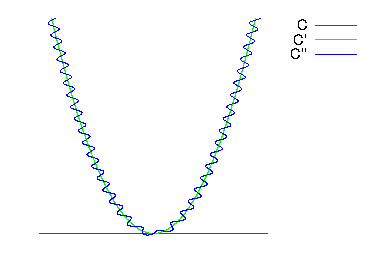
\includegraphics{x_squared_colour.pdf}
 \caption{An example for transformations.
   $\C$ represents a co-ordinate axis which is then transformed into a
 parabola, $\C^\prime$.  Finally a sinusoid is set about this
 $\C^\prime$ which give  $\C^\dprime$.
 Determining this function is a nice toy example to demostrate the
 power of geometric calculus.
}
 \label{fig:example_plots}
\end{figure}
Let us put these techniques to use in a simple example.
We begin with a curve embedded in a two dimensional Euclidean space,
and denote this curve $\C$.
%This curve will take the role of the `x-axis' in this discussion.
We then transform this into a second curve $\C^\prime$,
drawn so that $\C^\prime$ is a parabola with respect to $\C$.
%In the two dimensional space we are considering, 
When $\C$ is a straight line that takes a role of the `x-axis',
the curve $\C^\prime$ corresponds to the graph `$x^\prime = f(x) = x^2$'.
%, the axis with respect to which we are drawing the transformation.
We continue by drawing a third curve $\C^\dprime$,
which is a sinusoidal variation of $\C^\prime$. 
That is, we wish to draw the graph `$f^\prime(x^\prime) = \epsilon \sin(\abs{x^\prime})$' where
$\epsilon$ is a constant and $\abs{x^\prime}$ is the distance along
the curve $C^\prime$.
This example  will help to demonstrate how geometric calculus can be used to simply
solve problems that are far from trivial using coordinate methods.
The curves are drawn in \figref{example_plots}.  
It is our task to explicitally calculate their parameterisation.





% We consider a simple example.
% We wish to plot the two graphs of \figref{example_plots}.
% The first of these is the curve $\C^\prime := y^\prime = x^2$,
% while the second, $\C^\dprime$,  plots a sinusoidal variation about $y^\prime$.
% That is the sinusoid follows the bend in $y^\prime$.

% Implicit in the definition of $\C^\prime$ is an underlying coordinate basis,
% namely a Euclidean basis 
% \eql{
% {\gamma_i} = \{\gg, \ggg\}
% }{Euclidean_basis}
%  where
% $\gamma_i \cdot \gamma_j = 1$ if $i=j$ and $0$ otherwise.
% Then $y^\prime$ is the coordinate along the $\ggg$ axis,
% and $x$ is the coordinate along the $\gg$ axis.
% For curve $C^\prime$ such a basis enables the function to be expressed very
% simply.
% To represent $C^\dprime$ in such a basis is less convenient.

% Geometric algebra helps even in this simple example by letting much of
% the analysis to be done in a coordinate free manner.
% Then at the end,
% for the purposes of plotting the graph,
% we can introduce a convenient basis.







% Our graph can be expressed as a set of curves ${\C_i}$ embedded within a
% Euclidean two dimensional space spanned by the pseudoscalar $i$.
% For the purposes of drawing a graph we need a reference curve, $C$, 
% that takes the role of the `x-axis' in co-ordinate methods.

% Each of the curves are represented by a path
% \eq{
%   \C := x(\lambda) 
% }
% where $x$ is a vector intrinsic to the embedding space.
% Each of the curves can be considered as 1-dimensional vector manifolds
% within the 2-dimensional embedding space.
% If $p$ and $q$ are two points on the curve $\C_i$ then
% the vector $q-p$ is a chord of $\C_i$ from $p$ to $q$.
% In the limit the chords define a tangent vector to the curve so
% that  vector $a(x)$ is a tangent to a curve $\C$ at the point $x$ if
% \eq{
% a(x) = a\cdot \d x \equiv \left.\frac{dx(\lambda)}{\d \lambda}\right|_{\lambda =0}
% = \lim_{\lambda\rightarrow 0} \frac{x(\lambda) - x}{\lambda}.
% }
% The path can be reparameterised by the lengths of its cords,
% $\tau(\lambda) \equiv \abs{x(\lambda) - x}$,
% so that
% \eq{
% a = \frac{d\tau}{d\lambda} \frac{dx}{d\tau}.
% }
% The magnitude and unit direction of the tangent can then be identified
% as
% \eqal{
% \abs{a} = \frac{d\tau}{d\lambda} &,& \hat{a} = \frac{dx}{d\tau} = \frac{dx}{\abs{dx}},
% }{tangent_magnitude_and_unit}
% respectively.
% The unit tangent
% \eqa{
% v =\hat a =  \frac{dx}{d\tau} &,& v^2 = 1,
% }
% is known as the {\em velocity} of the curve.

% The parameter $\tau$ is unique to the curve in that we can identify $d\tau =\abs{dx}$.
% It follows that we can define a parameterisation-independant
% interval $(d\tau)^2 = dx\cdot dx$,
% which upon reintroducing an arbitrary parameterisation gives
% \eqal{
%  \left(\frac{d\tau}{\lambda}\right)^2 = \frac{dx}{d\lambda}\cdot\frac{dx}{d\lambda}.
% }{differential_length}
% The length of an arc on the path can be then be found to be
% \eql{
% \Delta \tau = \int_{\lambda^\prime}^{\lambda^\dprime}\left(\frac{dx}{d\lambda}\cdot\frac{dx}{d\lambda}\right)^{\half}d\lambda,
% }{defn_length}
% which is again invariant to a reparametrisaton.


When we draw a graph we follow the `independent-axis' to a given point,
and then leave that axis in the orthonal direction a distance determined
by some function, $\beta(x)$.
So by representing the independent-axis as a manifold (for example, the curve
$\C$ in the 2-dimensional case),
the map to the second manifold  is represented
\eql{
f: a \rightarrow a^\prime = f(x) = x + \beta(x) n(x),
}{graph_function}
where $x$ points to a point on the  manifold, and $n(x)$ is a vector entirely extrinsic (normal)
to the manifold at $x$. % so that $x\codt n = 0$.
The normal vector is defined to be the dual of the local-pseudoscalar on
the manifold, $I(x)$, such that
\eql{
  I(x) = n(x)i.
}{normal_definition}
The transformation of \eqnref{graph_function} is considered for arbitrary multivectors in
arbitrary dimensions by
\cite{Hestenes1984}.
Howerver, for our perposes the soley vectorial scope of
\eqnref{graph_function} are sufficient.
Since the pseudo-scalar to a curve is its velocity \eqnref{normal_definition}
reduces to
\eq{
  n(x) = v(x) i.}


Writing the transformation we seek is then easy,
\eqa{
  x^\prime = f(x) = x + \beta(x) v(x)i &,& \beta(x) &= x^2, \label{eqn:beta_zero}\\
  x^\dprime = f^\prime(x^\prime) = x^\prime + \beta^\prime(x^\prime) v^\prime(x^\prime)i &,& \beta^\prime(x^\prime) &= \sin(2\pi\omega\Delta\tau), \label{eqn:beta_one}
}
where $\Delta \tau$ is evaluated for position $x^\prime$ using \eqnref{defn_length}.

To plot \eqnref{beta_one} the velocity $v^\prime$ of $\C^\prime$ is
requred.
To obtain the tangent vectors to $\C^\prime$ from the tangent vectors
of $\C$ the  directional derivative,
$\fbar(a)= a\cdot\d f(x)$, is required.
Applying this to \eqnref{beta_zero} while remembering that $\d_x$ is the differential intrinsic to the curve $C$,
and so leaves alone the vector $n(x)$, gives
\eq{
 \fbar(a) = a + 2a\cdot x n. %\\
% \fbar^\prime(a^\prime) &= a^\prime + 2\pi\omega \cos(2\pi\omega\Delta \tau)\d\Delta \tau.
}
Remembering that the velocity is a curve's pseudoscalar and using
\eqnref{Jacobian} we obtain
% \eq{
% \fbar(v) = J_f v^\prime.
% }
% This can also be seen through use of the chain rule
% \eq{
% v^\prime(x^\prime) = \frac{dx^\prime}{d\tau^\prime} =
% \frac{d\tau}{d\tau^\prime}\frac{dx}{d\tau} \cdot\d f  = \frac{1}{J_f}\fbar(v). %&,&v^\dprime(x^\dprime) = \fbar_2(v^\prime),
% }
% So 
\eqa{
\fbar(v) &= v + 2 v\cdot x n = J_f v^\prime. \label{eqn:ExFbar}\\
\intertext{Upon squaring this leaves}
\left(\fbar(v)\right)^2 &= 1 + 4 \left(v\cdot x\right)^2 = J_f^2,\\
\intertext{and so the Jacobian of the transformation is given by}
 J_f &= \sqrt{ 1 + 4 \left(v\cdot x\right)^2 }. \label{eqn:ExJacobian}
}

Although it is not needed in this example it is worthwhile explicitly
calculating the adjoint function,
% The function
% \eq{
%  a^\prime = \fbar(a) =  a\cdot \del_x f(x)
% }
% maps the tangent vector $a(x)$ to the curve $C$ at the point $x$ to the
% tangent vector $a^\prime(x\prime)$ to the curve $C^\prime$ at the point
% $x^\prime$.
% Note that $\del_x$ is the differential intrinsic to the curve $C$,
% and so leaves alone the vector $n(x)$.
% Therefore we can write
% \eq{
% v^\prime(x^\prime) = \frac{dx^\prime}{d\tau} = \frac{dx}{d\tau} \cdot\d f  =\fbar(v). %&,&v^\dprime(x^\dprime) = \fbar_2(v^\prime),
% }
% Applying to \eqnref{beta_zero} and \eqnref{beta_one} gives
% \eq{
%  \fbar(a) = a + 2a\cdot x n, %\\
% % \fbar^\prime(a^\prime) &= a^\prime + 2\pi\omega \cos(2\pi\omega\Delta \tau)\d\Delta \tau.
% }
%Using
\eqa{
\fadj(a^\prime)& = \d_a \fbar(a) \cdot a^\prime \\
 &= \d_a  \left( a + 2a\cdot x n\right) \cdot a^\prime\\
 &= P(a^\prime + 2x n\cdot a^\prime),
}
where we are projecting onto $\C$.
Then
\eqa{
  \fadj\fbar(v) &= P\left( v + 2 v\cdot x n  + 2x n\cdot \left( v + 2 v\cdot x n \right)\right)\\
&= P\left( v + 2 v\cdot x n + 4x v\cdot x \right) v v \\
&= \left(  1 +  4 (v\cdot x)^2 \right) v \\
&= J_f^2 v,
}
as expected.

To actually plot the graphs we need to define a coordinate system for
the embedding space.
Using the Euclidean space defined in \eqnref{Euclidean_basis}
we may define the pseodoscalar of the 2-dimensional space as
\eq{
 i = \gg\ggg.
}
Setting the origin to be on the curve $C$ we choose
$v(x) = \gg$.
This implies that $n(x) = \gg i = \ggg$.
That is, the curve 
\eql
{
 \C : x(\tau) = \tau \gg
}{C_defn}
 is the `x-axis' for our graph,
and the normal is the `y-axis'.

Subsitutiong \eqnref{C_defn} into \eqnref{ExJacobian}
gives
\eqa{
  J_f &=  \sqrt{ 1 + 4\tau^2 }\\
\intertext{and so}
v^\prime &= \frac{\gg + 2\tau \ggg}{\sqrt{ 1 + 4\tau^2 }},
\intertext{where \eqnref{ExFbar} has been used.
Calculating $n^\prime$   with \eqnref{tau_primed} gives:}
 n^\prime = v^\prime i &=\frac{\ggg - 2 \tau\gg}{\sqrt{1+4\tau^2}}.
}
% where \eqnref{ExFbar} has been used.
% Calculating $n^\prime$  explicitly:
% \eql{
%   n^\prime = v^\prime i =\frac{\ggg - 2 \tau\gg}{\sqrt{1+4\tau^2}},
% }{n_primed}
% where we have used \eqnref{tau_primed}
% Next we define a basis for the curve $\C^\prime$,
% \eq{
%   e_i \equiv \fbar(\gamma_i)
% }
% and find
% \eqa{
%   e_1(\tau) = v^\prime(\tau) =J_f v^\prime(\tau^\prime) = \gg + 2\tau \ggg &,&e_2 \ne n^\prime =  \ggg.
% }
% Writing 
% \eq{
% v^\prime(\tau^\prime) = \frac{dx^\prime}{d\tau^\prime} =
% \frac{d\tau}{d\tau^\prime}\frac{dx^\prime}{d\tau} =
% \frac{d\tau}{d\tau^\prime}v^\prime(\tau) = 
% J_f v^\prime(\tau)
% }
% and enforcing $v^{\prime 2}(\tau^\prime) = 1$ gives
% \eq{
% v^\prime(\tau^\prime) = \frac{v^\prime(\tau)}{\sqrt{1+4\tau^2}}.
% } 
% %Writing $\tau^\prime = \epsilon \tau$ gives
% %\eq{
% %  v^\prime(\tau^\prime) = \epsilon \gg + 2\epsilon\tau\ggg,
% %}
% %and enforcing $v^{\prime 2} = 1$ implies that
% %\eql{
% % \tau^\prime = \frac{\tau}{\sqrt{1+4\tau^2}}.
% %}{tau_primed}
% Calculating $n^\prime$  explicitly:
% \eql{
%   n^\prime = v^\prime i =\frac{\ggg - 2 \tau\gg}{\sqrt{1+4\tau^2}},
% }{n_primed}
% where we have used \eqnref{tau_primed}
All that is required now is to find $\delta \tau$ between the origin and
$x^\prime$,
\eqa{
\Delta \tau &= \int_0^{\tau_\text{max}} \sqrt{ \fbar(v)\cdot \fbar(v)}d\tau 
 = \int_0^{\tau_\text{max}} \sqrt{1 + 4\tau^2  } d\tau\\
 &= \frac{1}{4} \left[
    \ln\left( 2\tau_\text{max} + \sqrt{1 + 4\tau_\text{max}^2 } \right) + 2\tau_\text{max} \sqrt{1 + 4\tau_\text{max}^2  }
\right] \label{eqn:example_delta_time}\\
&= \frac{1}{4} \left[ \ln\left( 2\tau_\text{max} + J_f \right) + 2\tau_\text{max} J_f \right]
}
where the standard identity $\cosh\sinh^{-1}(x) \equiv \sqrt{1+x^2}$ has
been used to put the integral in the form of \eqnref{example_delta_time}.

Pulling this together with the help of \eqnref{beta_zero} and \eqnref{n_primed},  we find
\eqa{
\C: x(\tau) &= \tau \gg\\
  \C^\prime: x^\prime(\tau) &= \tau \gg + \tau^2 \ggg \\ 
\C^\dprime: x^\dprime(\tau) &=  \tau \gg + \tau^2 \ggg  +
\epsilon J_f^{-1}\sin(2\pi\omega\Delta\tau) \left(\ggg - 2 \tau\gg\right)\nonumber \\
  &= \left(\tau - 2\tau\epsilon J_f^{-1}\sin(2\pi\omega\Delta\tau)
  \right) \gg 
    + \left(\tau^2 + \epsilon J_f^{-1}\sin(2\pi\omega\Delta\tau) \right) \ggg,
}
which is what is drawn in \figref{example_plots}.

Note that this example was straightforward using geometric algebra.
The interpretation of the quantities that were being evaluated at each
stage was clear, and by choosing a co-ordinate system at the end,
after the transformations had beed identified, the actual calculations
were short.
This would not have been the case for standard coordinate methods.
For instance, standard differential geometry does not keep track of
the extrinsic geometry to a manifold, and so our use of the normal
vector would require the introduction of a `fibre bundle',
with all the book-keeping that this would entail.




% As a first step we must invert
% \eq{
%   x^\prime(\tau) = \tau \gg + \tau^2 \ggg
% }
% The inequality of $e_2$ with $n^\prime$ is required so that the space


% To find the 
% The velocity of $\C^\prime$ is equal to the 

% We need a transformation to map between the curves
% A graph is simply a surface representing the height 

%   `dependent-variable' plotted
% orthogonally to a set of 
% 'independant-variables'.
% This can be achieved geometrically by transforming the surfance
% representing the indpedent variables into by reprenting each curve by a manifold.

% plotting a dependent-manifold
% tranformed ind
% representing the indepedent
% variables with a manifold which is transformed in the direction of a
% normal vector that is entirely extrinsic to the manifold.


% the manifold (in this case a curve) to represent the indepedent
% varibles we can define a normal vector $n$ that is entirely extrinsic to
% the manifold.
% In this case the normal vector at a position $x_\mu$ on curve $\C_\mu$ is
% \eq{
% n_\mu(x_\mu) = v(x_\mu) i.
% }



% A point in a graph should relate to its various axes via a projection.
% That is 
% a point $x_1(\tau_1)$ on $\C_1$ should map to the point $x(\tau)$ on $\C$
% by projection.
% That is
% \eq{
% f_1^{-1}: x_1 \rightarrow x = f_1^{-1}(x_1) = P(x_1)
% }

% where $P_{\C}(\cdot)$ reprents a projection operation onto the curve $C$.
% The appropriate projection operator is


% To map from $\C\rightarrow\C_1$ we should move along the curve $\C$
% to a position $x$,
% then we should 

% saying that
% the `dependent-variable' should sit  should
% and we can include this is a co
% For drawing a graph the notion of orthogonality between 
% The notion of othogonality between 
% Let us consider the transformation between the curves
% \eq{
%  f(x) = x + \beta(x) xi.
% }
% This function 


% with respect to which the curve $\C_1$ will be
% drawn, $\C$ takes the role of the `x-axis' in co-ordinate methods.


% The curve $C_1$ is then a mapped from $C$ via the transformation
% \eq{
%  C
% }

%  of two functions.
% Firstly, 
%  simple function $\beta(x) = x^2)$ with respect to a



%  of where we want to plot a 
% \eqa{
% x^\prime &= f(x) = x + \beta(x)n\\
% x^{\dprime}&= g(x^\prime) = g(f(x))  = x^\prime + \beta^\prime(x^\prime) n^\prime
% }
% where
% \eqa{
% x &= \lambda e_1\\
% n &= \hat x i \\
% n^\prime &= \hat \fbar(x) i \\
% i &= e_1 e_2
% }
% where for the purpose of the example 
% \eqa{
% \beta(x) &= x^2 \\
% \beta^\prime(x^\prime) &= \sin(x^\prime\cdot\fbar(e_1))
% }
% so that
% \eqa{
% a \cdot \d_x x^\prime = \fbar(a) &= a + a\cdot \d_x \beta(x) n\\
% &= a + 2 a \cdot x n
% }
% and
% \eqa{
% a\cdot \d_{x^\prime}x^\dprime = \underbar{g}(a^\prime) &=
%   a^\prime + a^\prime \cdot \d_{x^\prime}
%   \beta^\prime(x^\prime)n^\prime\\ 
% &= a^\prime + a^\prime \cdot \cdot\fbar(e_1)  \cos(x^\prime\cdot\fbar(e_1))
% }
% So
% \eqa{
% x^\prime = f(\lambda e_1) &= \lambda e_1 + \lambda^2 e_2 \\
% \fbar(e_1; \lambda) &= e_1 + 2 \lambda e_2
% }
% setting $a^\prime = \fbar(e_1)$
% \eqa{
% g(x^\prime) &= x^\prime + \sin(x^\prime \cdot f(e_1)) n^\prime \\ \nonumber
% &=\left[\lambda(1 - \lambda\sin(\lambda(1+2\lambda^2)))\right]e_1 \\ 
% &+ \left[\lambda(\lambda + \sin(\lambda(1+2\lambda^2)))\right]e_2\\
% }
% and 
% \eqa{
% \underbar g(\fbar(e_1)) &= 
% \fbar(e_1) + \fbar^2(e_1)\cos(\fbar^2(e_1)) \fbar(e_1)e_1e_2 \\ \nonumber
% &= \left[1 - 2\lambda(1+\lambda^2)\cos(1+\lambda^2)  \right]e_1 \\ &+
%    \left[2\lambda + (1 + 4\lambda^2)\cos(1+4\lambda^2)\right]e_2
% }

\subsection{Functional Derivative}
% The "bracket thing" is an inner product for functions (more generally distributions which are formal functions define only inside integrals and not necessarily in terms of values, as e.g. the Dirac delta "function")

% But there is a problem with your invocation of the chain rule. The functional $\mathcal{F}$ maps functions to scalars. If you assume $\rho$ is again a functional then you can't compose it with $\mathcal{F}$

% In general you can't compose functionals since their domain and range are distinct types (functions vs numbers).

% So you can either have a chain rule of the form:
% \eq{
% \frac{\delta\mathcal{F}[\rho(\sigma)]}{\delta \sigma}= \frac{\delta \mathcal{F}[\rho]}{\delta \rho}\frac{d \rho}{d \sigma}
% }
% Or invoke a parameterized functional (functional valued function) which will give a much messier chain rule.

% It may help (though not I think to prove the general case) to start
% with functionals defined by integrals, i.e.:
% \eq{
% \mathcal{F}[\rho] \equiv \int \phi(\rho(x))dx
% }
% then you get functional differential:
% \eq{
% \delta \mathcal{F}[\rho] = \int \frac{d \phi(\rho)}{d\rho}\delta \rho dx
% }
% Then the functional derivative (as a distribution) is:
% \eqa{
% \left\langle \frac{\delta \mathcal{F}[\rho]}{\delta\rho} , f\right\rangle=\int\frac{d \phi(\rho)}{d\rho} f dx
% \intertext{thence}
% \frac{\delta \mathcal{F}[\rho]}{\delta\rho} =\frac{d \phi(\rho)}{d\rho}= \phi' \circ \rho
% }
% In standard calculus you will note that the derivative of a function is a multiplier for a linear term in the variable. The n-th derivative is the multiplier for an n-th degree term. Effectively then the first derivative times the variable is a linear function, and higher order n-th degree functions.

% In the functional case, the first functional derivative contracts with
% the variable (a function) to yield a linear functional. This is why
% you get a "distribution" instead of a function. Because the space of
% functions is infinite dimensional, its dual space consists of more
% than linear functionals of the form:
% \eq{
% f \mapsto \left\langle \phi , f \right\rangle
% }
% where $\phi$ is a function. We must define a more general class of objects, distributions which are only defined by first giving a linear functional and then rewriting it in the form of an inner product above but with the $\phi$ not meaningful as an actual function.

% Note you can generalize further by considering an operator (not necessarily linear) which maps functions to functions and for which we can (with some restrictions) define an operator derivative
% \eq{
% \frac{\Delta \Omega[\phi]}{\Delta \phi}
% }
% as an linear operator (for a given $\phi$).

% Thence:
% \eq{
% \frac{\Delta \Omega[\phi]}{\Delta \phi}[a \xi + b \eta] =a\frac{\Delta \Omega[\phi]}{\Delta \phi}[\xi] +b\frac{\Delta \Omega[\phi]}{\Delta \phi}[\eta]
% }
% is a function. (a and b scalars, f and g functions.)

% Since you can compose operators you can then better discuss an operator chain rule:
% \eq{
% \frac{\Delta \Omega[\Xi[\psi]]}{\Delta \psi}[f] = \frac{\Delta \Omega[\Xi[\psi]]}{\Delta \Xi}\left[\frac{\Delta \Xi}{\Delta \psi}[f]\right]
% }
% In essence one generalizes the Taylor expansion of a general operator
% in terms of "constant" plus linear operator plus bilinear operator ...



% I noticed that I didn't actually give you the definition of the operator derivative. It is defined as a linear operator such that for small variations of the function:
% \eq{
% \Omega[f+\delta f] = \Omega[f]+ \frac{\Delta\Omega[f]}{\Delta f}[\delta f] + O(\delta f^2)
% }

% To get more rigorous:
% \eq{
% \Omega[f+\delta f](x) = \Omega[f](x)+ \frac{\Delta\Omega[f]}{\Delta f}[\delta f](x) + O(\delta f^2)
% }
% where the order of the square of the variation is defined by taking the maximum magnitude of $\delta f(x)\cdot \delta f(y)$ for all values of x and y.

% You can then define the derivative explicitly by:
% \eqa{
% \frac{\Delta\Omega[f]}{\Delta f}[\delta f](x) = \lim_{\epsilon\to 0}\\
% \frac{\Omega[f + \epsilon\delta f](x)-\Omega[f](x)}{\epsilon}
% }
% where $\delta f$ is any of a restricted class of functions e.g. test functions or bounded smooth functions with compact support or something similar.

% Here is a clarifying example.

% The derivative of a function is the action of an operator $\mathbf{D}$ on that function.

% We can thus take the operator derivative of the differential operator:
% \eq{
% \mathbf{D}'[f] = \frac{\Delta \mathbf{D}[f]}{\Delta f}
% }
% Since we are taking an operator derivative $mathbf{D}'[f]$ will be a linear operator. But since the derivative is a linear operator its derivative will be a constant (with regard to f).

% In short $\mathbf{D}'[f_1] = \mathbf{D}'[f_2]$.

% So the "value" of the "derivative of the derivative" is:
% \eq{
% \mathbf{D}'[f][g]= \lim_{\epsilon\to 0}\frac{\mathbf{D}[f+\epsilon g]-\mathbf{D}[f]}{\epsilon}
% =\lim_{\epsilon\to 0} \frac{\mathbf{D}[f] +\epsilon\mathbf{D}[g]-\mathbf{D}[f]}{\epsilon} = \mathbf{D}[g]
% }
% So the "derivative of the derivative" is "the derivative" in the same sense that the derivative of f(x)=cx is c viewed as a linear multiplier.

% It may help more to think of the operator derivative as acting like a Greens function:
% The derivative being linear can be expressed as an integral:
% \eq{
% \mathbf{D}[f](x) = \int \delta'(x-y)f(y)dy
% }
% where $\delta'(x-y)$ is the formal derivative of the Dirac delta function (limit of derivatives of normalized Gaussian functions as the variation goes to zero).


% The derivative then is the linear operator defined in "component form" by the two valued function $D(x,y) = \delta'(x-y)$. Think of the variables as acting analogous to the indices of vectors or matrices.

% You can think of the higher order functional and operator derivatives as generalized Taylor expansions:

% For functionals:
% \eq{
% \mathcal{F}[\phi] = F^{(0)}+ \int F^{(1)}(x)\phi(x)dx + \iint F^{(2)}(x,y)\phi(x)\phi(y) dx dy + \iiint F^{(3)}(x,y,z)\phi(x)\phi(y)\phi(z)dx dy dz + \cdots
% }
% For operators:
% \eq{
% \Omega[\phi](x) = \Omega^{(0)}(x) + \int \Omega^{(1)}(x,y)\phi(y)dy + \iint \Omega^{(2)}(x,y,z)\phi(y)\phi(z) dy dz + \cdots
% }
% where these "multi-variable functions" $\Omega^{(k)}$ are rather multi-distributions since they only appear in integrals.



The functional $F[\genf]$ is to be minimised,
that is, we wish to find the function $\genf$ that remains invarient
under the transformation $\genf \rightarrow \genf + \epsilon g$, where
$\epsilon$ is a small constant and $g$ is an arbitrary function.



From \cite{Lasenby1993} we have:

Want to evaluate
\eq{
  \d_{\fbar(b)} \fbar(A_r)
}
where
\eq{
 \fbar(b) = b\cdot \del f(x)
}
and so assume that we evaluate differential at the same point $x$.

First project $A_r$ onto the vector $b$,
\eq{
 P_b (A_r) = (A_r\cdot b^{-1}) b = b\wedge(b^{-1}\cdot A_r),
}


It can be conceptually useful to discretise the input to the function
into an
%
%the function $\genf$ into an
%$N$ dimensional vector, paramameterised by the 
$N$ dimensional Cartesian
basis $e_n$, $n = 1, 2, \ldots, N$:
\begin{align}
& \genf \rightarrow \genf_j  \equiv \genf(e_j), &g \rightarrow g_k  \equiv g(e_k) &
\end{align}
The components of the vector can be found by contracting with the basis,
\begin{align}
 g_{ik} \equiv  e_i \cdot g_k
\end{align}

%where $\genf_j$ is the $j^{th}$ component of the vectorised function
%$\genf$.
The continuum limit can be recovered later by letting
$N\rightarrow\infty$.



A set of $N$ directional derivaties can then be evaluated in the usual
way,
\begin{align}
 g_k \cdot \d_{\genf_j} F( \genf_j ) &= \lim_{\epsilon \rightarrow 0} \frac{1}{\epsilon}
   \left( F( \genf_j + \epsilon g_k)  - F( \genf_j )  \right)
\\
e_i \cdot \d_{\genf_j} F( \genf_j ) g_{ik} &=\lim_{\epsilon \rightarrow 0} \frac{1}{\epsilon}
   \left( F( \genf_j + \epsilon e_i)  - F( \genf_j )  \right)g_{ik},
\end{align}
where we are summing over the repeated index $i$.
The derivative over the discretised function $f$ is then the sum over
these $N$ directional derivatives,
\begin{align}
 dF &=  \sum_k^N g_k \cdot \d_{\genf_j} F(\genf_j) 
 \label{eqn:vectorized_functional_derivative}
\end{align}
The right hand side can be simplified by making the following
definition,
\begin{align}
e_i \cdot \d_{\genf_j} = \d_{e_i \cdot \genf_j} \equiv \d_{\genf_{ij}},
\end{align}
so that \eqnref{vectorized_functional_derivative} can be written
\begin{align}
 dF &=  \sum_{k}^N \d_{\genf_{ij}} F(\genf_j) g_{ik}.
\end{align}

From \cite{Doran2003},
\begin{align}
 f_{ij} = e_i \cdot \genf(e_j).
 \end{align}
so that
\begin{align}
 \d_{f_{ij}} \genf(b)\cdot c &= \d_{f_ij} (\genf_{lk} b^k c^l) \\
 &= c^i b^j
\end{align}
So mulitplying by $a\cdot e_j e_i$ we get
\begin{align}
 a\cdot e_j e_i \d{\genf_{ij}} \genf(b)\cdot = a \cdot b c,
\end{align}

so
\begin{align}
 \d_{\genf(a)} = a\cdot e_j e_i \d_{f_{if}}
\end{align}
so that 
\begin{align}
 \d_{\genf(a)} \genf(b)\cdot c = a\cdot b c
\end{align}

In general we have
\begin{align}
  \d _{\genf(a)} \scalar{\genf(A)B} = \sum_r \mono{\genf(a\cdot A_r)B_r}
\end{align}
so that for a fixed grade multivector we can write
\begin{align}
 \d_{\genf(a)} \genf({A_r}) = \left(n-r+1\right)\genf(a\cdot A_r)
\end{align}

Use in the Euler Lagrange Equations:
\begin{align}
\frac{\d}{\d\genf(e^j)} &= e_i \frac{\d}{\d \genf_{ij}}
\end{align}

If
\begin{align}
\genf(a) = a\cdot \d f(x) 
\end{align}
then
\eq{
  \genf_{ij} = e_i \cdot \genf(e_j) = e_j \cdot (\d_i f)
}
so that
\eq{
\frac{\d}{\d(\d_j f)} = e_j \frac{\d}{\d_{\genf_{ij}}}= \frac{\d}{\d\genf(e^j)}
}


%\section{Lagrangian Mechanics}




Mostly taken from \cite{Lasenby1993}.
The scalar valued function 
\eq{
L = L(\psi_i, \dot{\psi}_i),
}
where $\psi_i$ are a set of general multivectors.

Extremise the action
\eq{
S = \int_{t_i}^{t_f} dt L(\psi_i, \dot{\psi}_i)
}
with respect to $\psi_i$.
We write 
\eq{
 \psi_i(t) = \psi_i^0(t) + \epsilon \phi_i(t)
}
where $\phi_i$is a multivector of the same grades as $\psi_i$,
$\epsilon$ is a scalar and $\psi_i^0$ represents the extremal path.

Take the derivative wrt $\epsilon$ to get
\begin{align}
  \d_\epsilon L &= \int_{t_i}^{t_f} dt \left( 
    \phi_i \ast \d_{\psi_i} L + \dot{\phi}_i\ast \d_{\dot{\psi}_i} L
    \right)\\
&= \int_{t_i}^{t_f} dt  
    \phi_i \ast \left(\d_{\psi_i} L - \d_t( \d_{\dot{\psi}_i} L) \right)
+
\left[ \phi_i\ast\d_{\dot{\psi}_i } L  \right]_{t = t_i}^{t = t_f}
\end{align}
For stationarity this must vanish for all $\phi_i$,
giving the Euler-Lagrange Equations
\eq{
\d_{\psi_i} L - \d_t(\d_{\psidot_i}L) = 0
}

\subsection{Transformation}
Consider transformation parameterised by a single multivector $M$
\eq{
 \psi_i^\prime = f(\psi_i, M)
}
where $f$ and $M$ are time independent.

Define:
\eq{
  \fbar_A(\psi_i, M) = A\ast \d_M f(\psi_i, M)
}
and
\eq{
L^\prime = L(\psi_i^\prime, \psidot_i^\prime)
}
gives
\begin{align}
A\ast\d_M L^\prime &=
 \fbar_A(\psi_i, M) \ast \d_{\psi_i^\prime} L^\prime + 
 \fbar_A(\psidot_i, M) \ast \d_{\psidot_i^\prime}L^\prime
\\
&= \fbar_A(\psi_i, M)\ast\left(\d_{\psi_i^\prime} L^\prime -
 \d_t(\d_{\psidot_i^\prime} L^\prime)\right)
+ \d_t\left(\fbar_A(\psi_i, M) \ast \d_{\psidot_i^\prime}L^\prime\right)
\end{align}
Assuming that the equations of motion are satisfied by $\psi_i^\prime$
gives
\begin{align}
A\ast\d_M L^\prime = \d_t\left(\fbar_A(\psi_i, M) \ast
 \d_{\psidot_i^\prime} L\right)
\end{align}
Differentate out the $A$ dependance
\begin{align}
 \d_M L^\prime &= \d_t \left( \d_A \fbar_A (\psi_i, M) \ast \d_{\psidot_i^\prime}L^\prime\right)
&= \d_t\left(\rd_M \psi_i^\prime \ast \d_{\psidot_i^\prime}L^\prime\right)
\end{align}

If $L^\prime$ is independent of M then
 $\d_A \fbar_A(\psi_i, M)\ast\d_{\psidot_i^\prime}L^\prime$ is
 conservered.

If $M$ is a scalar parameter, $\alpha$ then
\begin{align}
 \d_\alpha L^\prime = \d_t \left( (\d_\alpha \psi_i^\prime)\ast \d_{\psidot_i^\prime}L^\prime \right)
\end{align}
e.g.
\begin{align}
\psi_i^\prime(t,\alpha) &= \psi(t+\alpha)\\
\text{gives } \given{\d_\alpha \psi_i^\prime}{\alpha = 0} &= \psidot_i
\end{align}

If all $t$-dependance enters $L$ through the dynamical variables only we
get
\begin{align}
\d_t L = \d_t \left(\psidot_i \ast \d_{\psidot_i} L\right)
\end{align}
and the conserved Hamiltonian as
\begin{align}
 H = \psidot_i \ast \d_{\psidot_i}L - L
\end{align}

%\section{Field Theory}

The introduction of symmetry arguments is most easily accomplished
with field theory.
Additionally, the writing of dynamics into a single lagragnian means
that a self consistent set of contraints has been provided,
and in this sence makes a good check.

So we write a scalar lagragian $\L$ according to the zeroth and first
derivatives of a set of  multivector fields $\psi_i(x)$,
\eq{
\L = \L(\psi_i, \del \psi_i).
}
We wish to minimise the action
\eq{
S = \int\abs{d^4x}\L.
}
with respect to $\psi_i$ and so we write 
\eq{
\psi_i(x) = \psi_i^0(x) + \epsilon \phi(x),
}
where $\psi_i^0(x)$ is the minimal field.

To minimise we take the derivative with respect to $\epsilon$
\eq{
\d_\epsilon S = \int \abs{d^4x} \left(\phi\star\d_{\phi_i} \L + (\del
  \phi_i)\star \d_{\del \psi_i} \L\right).
}
The last term can be written
\eq{
 \scalar{\dot \del \dot \phi_i \d_{\del \psi_i} \L } = 
  \del\cdot\scalar{\phi_i \d_{\del \psi_i}\L} - \phi_i \star 
\left( (\d_{\del \psi_i} \L) \ldel \right)
}
assuming boundary vanish get
\eq{
 \d_\epsilon S = \int \abs{d^4x}\psi\star
\left(\d_{\psi_i}\L - (\d_{\del \psi_i} \L ) \ldel \right)
}
If $\psi_i$ contains only terms of grade-$r$ then the appropriate
Euler-Lagrange equations are
\eq{
\multi{\d_{\psi_i}\L - (\d_{\del \psi_i} \L) \ldel}{r} = 0,
}
wheras if $\psi$ is a general even multivector then
\eq{
\d_\psi \L = (\d_{\del \psi}\L) \rdel
}
%
%
%\section{Functional Differentiation}
%
%From \cite{Lasenby1993} we have:
%
%Want to evaluate
%\eq{
%  \d_{\fbar(b)} \fbar(A_r)
%}
%where
%\eq{
% \fbar(b) = b\cdot \del f(x)
%}
%and so assume that we evaluate differential at the same point $x$.
%
%First project $A_r$ onto the vector $b$,
%\eq{
% P_b (A_r) = (A_r\cdot b^{-1}) b = b\wedge(b^{-1}\cdot A_r),
%}
%
%
%
%The functional $F[\genf]$ is to be minimised,
%that is, we wish to find the function $\genf$ that remains invarient
%under the transformation $\genf \rightarrow \genf + \epsilon g$, where
%$\epsilon$ is a small constant and $g$ is an arbitrary function.
%
%It can be conceptually useful to discretise the input to the function
%into an
%%
%%the function $\genf$ into an
%%$N$ dimensional vector, paramameterised by the 
%$N$ dimensional Cartesian
%basis $e_n$, $n = 1, 2, \ldots, N$:
%\begin{align}
%& \genf \rightarrow \genf_j  \equiv \genf(e_j), &g \rightarrow g_k  \equiv g(e_k) &
%\end{align}
%The components of the vector can be found by contracting with the basis,
%\begin{align}
% g_{ik} \equiv  e_i \cdot g_k
%\end{align}
%
%%where $\genf_j$ is the $j^{th}$ component of the vectorised function
%%$\genf$.
%The continuum limit can be recovered later by letting
%$N\rightarrow\infty$.
%
%
%
%A set of $N$ directional derivaties can then be evaluated in the usual
%way,
%\begin{align}
% g_k \cdot \d_{\genf_j} F( \genf_j ) &= \lim_{\epsilon \rightarrow 0} \frac{1}{\epsilon}
%   \left( F( \genf_j + \epsilon g_k)  - F( \genf_j )  \right)
%\\
%e_i \cdot \d_{\genf_j} F( \genf_j ) g_{ik} &=\lim_{\epsilon \rightarrow 0} \frac{1}{\epsilon}
%   \left( F( \genf_j + \epsilon e_i)  - F( \genf_j )  \right)g_{ik},
%\end{align}
%where we are summing over the repeated index $i$.
%The derivative over the discretised function $f$ is then the sum over
%these $N$ directional derivatives,
%\begin{align}
% dF &=  \sum_k^N g_k \cdot \d_{\genf_j} F(\genf_j) 
% \label{eqn:vectorized_functional_derivative}
%\end{align}
%The right hand side can be simplified by making the following
%definition,
%\begin{align}
%e_i \cdot \d_{\genf_j} = \d_{e_i \cdot \genf_j} \equiv \d_{\genf_{ij}},
%\end{align}
%so that \eqnref{vectorized_functional_derivative} can be written
%\begin{align}
% dF &=  \sum_{k}^N \d_{\genf_{ij}} F(\genf_j) g_{ik}.
%\end{align}
%
%From \cite{Doran2003},
%\begin{align}
% f_{ij} = e_i \cdot \genf(e_j).
% \end{align}
%so that
%\begin{align}
% \d_{f_{ij}} \genf(b)\cdot c &= \d_{f_ij} (\genf_{lk} b^k c^l) \\
% &= c^i b^j
%\end{align}
%So mulitplying by $a\cdot e_j e_i$ we get
%\begin{align}
% a\cdot e_j e_i \d{\genf_{ij}} \genf(b)\cdot = a \cdot b c,
%\end{align}
%
%so
%\begin{align}
% \d_{\genf(a)} = a\cdot e_j e_i \d_{f_{if}}
%\end{align}
%so that 
%\begin{align}
% \d_{\genf(a)} \genf(b)\cdot c = a\cdot b c
%\end{align}
%
%In general we have
%\begin{align}
%  \d _{\genf(a)} \scalar{\genf(A)B} = \sum_r \mono{\genf(a\cdot A_r)B_r}
%\end{align}
%so that for a fixed grade multivector we can write
%\begin{align}
% \d_{\genf(a)} \genf({A_r}) = \left(n-r+1\right)\genf(a\cdot A_r)
%\end{align}
%
%Use in the Euler Lagrange Equations:
%\begin{align}
%\frac{\d}{\d\genf(e^j)} &= e_i \frac{\d}{\d \genf_{ij}}
%\end{align}
%
%If
%\begin{align}
%\genf(a) = a\cdot \d f(x) 
%\end{align}
%then
%\eq{
%  \genf_{ij} = e_i \cdot \genf(e_j) = e_j \cdot (\d_i f)
%}
%so that
%\eq{
%\frac{\d}{\d(\d_j f)} = e_j \frac{\d}{\d_{\genf_{ij}}}= \frac{\d}{\d\genf(e^j)}
%}




%%% Local Variables: 
%%% mode: latex
%%% TeX-master: "tshorrock_thesis"
%%% End: 

\part{Theoretical}\label{part:theory}


%%% Local Variables: 
%%% mode: latex
%%% TeX-master: "tshorrock_thesis"
%%% End: 


\chapter{Bubble Nucleation}\label{ch:nucleation}
%\begin{quote}
%\flushleft
%I had a little turtle \break
%His name was Tiny Tim \break
%I put him in the bathtub \break
%To see if he could swim. \break\break
%He drank up all the water \break
%He ate up all the soap \break
%Now he's stuck in bed \break
%with a bubble in his throat. \break\break
%Bubble, bubble, bubble, \break
%Bubble, bubble, bubble, \break
%Bubble, bubble, bubble, \break
%Bubble, bubble, POP!! 

%\flushright
% Nursery rhyme
%\end{quote}
%\begin{quote}

%Consider, for example, a crystal of Rochelle salt.
%For one set of experiments on it, we work with temperature, pressure and volume.
%The entropy can therefore be expressed as some function $S_e(T,P)$.
%For another set of experiments on the same crystal,
%we work with temperature, the component $e_{xy}$ of the strain tensor,
%and the component $P_z$ of the electric polarisation;
%the entropy as found in these experiments is a function $S_e(T, e_{xy}, P_z)$.
%It is clearly meaningless to ask ``What is the entropy of the crystal?''
%unless we first specify the set of parameters which define its thermodynamic state.%
%
%One might reply that in each of the experiments cited, 
%we have used only part of the degrees of freedom of the system,
%and there is a ``true'' entropy which is a function of all these parameters simultaneously.
%However we can always introduce as many parameters as we please...
%There is no end to this search for the ultimate ``true'' entropy until we have reached the point where we control
%the location of each atom independently.
%But just at that point the notion of entropy collapses, and we are no longer talking thermodynamics!
%
%From this we see that entropy is an anthropomorphic concept,
%not only in the well known statistical sense that it measures the extent of human ignorance as to the microstate.
%{\em Even at the purely phenomenological level, entropy is an anthropomorphic concept.}
%For it is a property, not of the physical system,
%but of the particular experiments that you or I choose to perform on it.
%
%\flushright Edwin T. Jaynes\cite{Jaynes1965}
%\end{quote}

%Conventional microbubble contrast agents are too large to be able to leave the blood
%and small bubbles are difficult to stabilise.
%This  limits their diagnostic applicability.
%One solution to this problem is to use an oil-droplet as the contrast agent.
%Oil droplets are inherently more stable at diameters of 


%The bubbles should not be generated haphazardly
%in the bodily  tissues (here assumed to be water)
%but rather formed selectively from an injected oil based  {\em contrast agent},
%which is vapourised when placed under a tension from an ultrasound induced negative pressure.
%In this chapter we review the theory behind the nucleation events that generate the bubbles.

\section{Introduction}
In this chapter we investigate theoretically the use of an ultrasound pulse to generate submicron bubbles.
Submicron bubbles are important because they
resonate at higher-frequencies, enabling imaging at higher resolutions;
and because 
%due to their size 
they are more likely to leave the blood than conventional micron-sized bubbles,
the crucial first step towards functional diagnostic contrast imaging.

Broadly, there are two approaches to acoustically generating a bubble:
\nlist
{
  \item produce a bubble from the bulk fluid directly.  
In medical ultrasound the bulk will invariably be some aqueous solution.
  \item introduce a second fluid, immiscible to the bulk, from which to generate bubbles.
%In medical ultrasound this involves introducing an emulsion 
This second fluid - an oil in the aqueous bulk - 
can be chosen with properties to facilitate the acoustic generation of a bubble.\label{item:nuc:oil}
}
Unfortunately, this division in methodology does not make clear the mechanisms
by which a bubble may be generated. % a more careful division in methodology is required.
%The difficulty with this division in methodology is that it does not bear close scrutiny.
The bulk fluid will, unless extraordinary efforts are undertaken,
contain small particles of dust that may or may not entrap pockets of gas,
contain gas bubbles stabilised with trace amounts of detergent,
in addition to containing a host of dissolved gases.
Likewise for any secondary fluid that is introduced,
with the additional complication of the water-oil interface 
becoming a rest point for other impurities in the system and 
developing a complex chemistry of its own.
%It will be seen in this chapter that
Bubble generation is extremely sensitive to the surface chemistry of a nascent bubble\cite{Talanquer2000},
while the presents of motes and existing bubbles can change the
mechanism of bubble generation entirely.
The presence of dissolved gasses is also known to be important in bubble generation\cite{Talanquer2001},
although this case is not investigated in this thesis.
%but  
%There are multiple mechanisms by which 




%There are a number of different mechanisms by which a gas bubble can be produced when 
%the pressure drops within a fluid.
Historically the term {\em cavitation} has been used ambiguously with respect to the mechanism of bubble formation. % upon a reduction in pressure within a fluid.
It is therefore helpful 
to instead use the word {\em nucleation} with the more careful categorisation of Jones\cite{Jones1999}:
\desc{
  \item[Type 1: classical homogeneous nucleation:]
     a bubble is {\em created} within the bulk medium where no bubbles were present prior to the reduction in pressure,
  \item[Type 2: classical heterogeneous nucleation:]
    a bubble is {\em created} upon a solid particle floating in the medium, or in a crevice in the surface of the container,
  \item[Type 3: pseudo classical nucleation:]
    a bubble results from a {\em pre-existing} but sub-critical gas cavity.
    The gas cavities may be stabilised by a crevice in a floating particle or by a crevice in  the container,
    or may be bubbles stabilised by a variably permeable skin\cite{Yount1979}.
    Sub-critical means that their curvature is smaller than the {\em critical radius}, 
    the radius at which the bubble is in equilibrium with its surroundings.
    The bubble  must still overcome an energy barrier to grow.
  \item[Type 4: non-classical nucleation:]
    a bubble results from a {\em pre-existing} gas cavity but there is no  energy barrier to growth.
    This occurs when the radius of curvature of a crevice is larger than the critical radius.
%    and multiple cavitation events generally occur from the same crevice.
    It is the lack of the energy barrier that makes this nucleation  non-classical.    
}


With these differing mechanisms in mind our two broad methodologies are revisited.
By what mechanism can the bulk fluid (water) be nucleated with ultrasound?
Is the mechanism the same in an oil emulsion?


\subsection{The nucleation of water}


The pressures required for water to undergo type I nucleation are prohibitive for diagnostic ultrasound.
Herbert\cite{Herbert2006} measured the nucleation probability to be vanishingly small at  \unit{-20}\mega\pascal,
with the probability rising to 50\% at \unit{-26}\mega\pascal, a result typical of  other measurements\cite{Hemmingsen1975}.
However, gas can be extracted from water at negative pressures at a few atmospheres\cite{Willard1953}.
Such nucleation events must result from another mechanism.
%Dissolved gasses or impurities within the water must therefore be the cause.

Motes %(particles of dirt within the water) 
promote nucleation by reducing the surface area of the vapour-liquid interface,
thereby reducing the energy required to form the bubble.
In the absence of entrapped gas - when the crevices are fully {\em wetted} with the bulk fluid -  type 2 nucleation occurs.
The reduction in the energy barrier can be considerable and is greatest when the crevices are deep and narrow\cite{Lubetkin1995}.
Herbert\cite{Herbert2006}, for instance, noted that while tap water has the same 50\% cavitation threshold as purified water,
%
%\footnote{To calculate the cavitation probability, 
%
%it is likely that any gas entrapped is removed from the motes within the water by earlier pulses.
%},
tap water has a very long tail of rarer nucleation events at much less extreme pressures.
Although not fully determined in the article, 
it seems reasonable to suggest that these events occur through type II nucleation:
Herbert uses repeated pulses that have negative pressures in excess of \unit{15}\mega\pascal\
and at such high pressures it is likely that gas entrapped in motes is removed 
by earlier pulses.
This would be consistent with a 50\% cavitation threshold that is identical to purified and degassed water,
a result that is hard to reconcile if there is entrapped gas within the system.

Nucleation events in human tissue are relatively rare,
%
%even at pressure in excess of \todo{need to find this study} \cite{}.
%Nucleation 
and do not become probable until the type I/II nucleation thresholds of water\cite{Webb1988}.
%Such pressures by far exceed the nucleation pressures recorded for free standing water.
Biology, it seems, is very adept at preventing gas pockets from occurring within tissue.




%However, deep and narrow crevices are also those that are most likely to entrap gas\cite{Lubetkin1995}
The high cavitation pressures recorded for type I and type II nucleation 
mean that the nucleation of impure water at diagnostic pressures is believed to proceed via type III and IV nucleation\cite{Atchley1989, Borkent2009, Jones1999}.
%Herbert also studied the nucleation probabil
%However, such crevices are not in general wetted, meaning that they entrap gas. % and so they usually undergo type 3 and 4 nucleation.
%For these reasons, the cavitation of water is generally believed to proceed via type 3 and 4 nucleation at diagnostic pressures\cite{Atchley1989, Borkent2009, Jones1999}.
There are two models for type III and IV nucleation. 
The first is that  partially wetted motes trap gas\cite{Atchley1989} and  the second is 
that  organic impurities  stabilise freely floating gas bubbles\cite{Yount1979}.
Both suggestions have been observed experimentally\cite{Borkent2009, Johnson1981}
and both are thought to be important in practice.

Due to the high cavitation pressures in biological tissues,
a medium that introduces Type III and IV nucleation events is a prime targets for developing a contrast agent.
These media have traditionally introduced stabalised micron sized bubbles.
% that have been 
%stabalised to various degrees of sophisication.
There is no reason why they should not, alternatively, introduce gas entrapped in motes,
such as are found in regular tap water.
%This possibility is investigated in this thesis
%along side a medium that contains oil droplets chosen for their cavitation properties.

%and so a technique that cavitates the bulk as well as the contrast agent will have limited use,
%irrespective of the lifetimes of the two types of bubble.

% The motes trap gas 
% The entrapment of gas within a crevice can be explained in terms of the initial wetting of the mote -
% the contact angle of partial wetting preventing the fluid reaching the bottom of the crevice.
% The model of Atchley and Prosperetti\cite{Atchley1989} has been successful in predicating the nucleation of bubbles on cylinders etched into a silicon wafer substrate\cite{Borkent2009}.
% The stabilisation of a dissolving bubble by organic solvents - in accord to the variable permeability model of Yount\cite{Yount1979} - 
% has been observed by Johnson and Cooke\cite{Johnson1981}.
% Which of these models dominate - the stabilised bubble or motes - is not certain.

%The cavitation of water therefore depends upon its cleanliness.
%The purity of tap water varies, but Apfel's\cite{Apfel1984} suggestion of \unit{$10^5$}\centi\metre\rpcubed,
%has been found to be useful\todo{Lookup where this figure has been used again}.

% If the water were distributed into droplets, or one mote per \unit{140}\micro\metre-radius droplet.
% The problem of a `dirty' fluid, therefore, can be eliminated by using small enough droplets.
% This is the basis of the droplet explosion technique\cite{HongChul2005} to calculate the investigate the super-saturation limit of a fluid\cite{Apfel1984}. 

%The cavitation properties of human tissue seem to be closer to that of type II nucleation.

%To give contrast it is necessary that the  bubble  formed from the droplet is distinguishable
%from other nucleation events that can occur in the bulk.
%This can occur if
%\nlist{
%  \item the  droplet, or gas within the droplet,  is induced to vapourise at a less negative pressure than the bulk;
%  \item the lifetime of the oil vapour bubble is longer than bubbles formed in the bulk.
%}
%The first is the most important.
%This is because the cavitation threshold of many human tissues approaches the type I/II nucleation thresholds\todo{cite}.
%Biology seems very adept at preventing gas pockets from occuring.
% cavitation is not without bio-effect
%and so a technique that cavitates the bulk as well as the contrast agent will have limited use,
%irrespective of the lifetimes of the two types of bubble.

\subsection{The nucleation of an oil droplet within an emulsion}


To leave the blood through leaky tumour vasculature the radius of a droplet must be at  most  \unit{300}\nano\metre\cite{Fukumori2006, Hashizume2000,  Hobbs1998}.
What is the likely nucleation mechanism for a droplet this small?
Let us first estimate the probability that the droplet contains a mote.

The probability that a droplet contains a mote depends both on the purity of the oil used to make up the droplets
and the purity of the surrounding medium.
We assume that the proportion of oil in the medium is small and that the impurities from the bulk dominate.
We also neglect any differences in the affinities of the oil and bulk to the mote.
Finally, we suppose that we make no special effort to either clean or dirty the water,
but instead take the water straight from the tap.
%This then provides an estimate of the importance of motes in the nucleation process,
For the mote-density of tap water we shall use Apfel's\cite{Apfel1984} suggestion  of \unit{$10^5$}\centi\metre\rpcubed.

From Apfel's density it follows that for every mote there will be
\begin{align}
\frac{1}{\text{motes per volume}\times\text{volume per droplet}} = 10^8
%\frac{1}{10^11 * \frac{4}{3}\pi \lr{3\times10^-7}^3} =
\end{align} 
droplets with a radius of \unit{300}\nano\metre.
Since a pre-existing gas bubble (stabalised or not) would have to be exceptionally small to be trapped within \unit{300}\nano\metre\ oil droplet,
%and since mote-induced cavitation is not found to be dominated by a vastly higher density of existing bubbles,
we conclude that  the oil droplets of interest are  likely to undergo type I nucleation.
Indeed, the use of small droplets to avoid the problems of `dirty' water is  a well used technique for experimentally investigating type I nucleation\cite{Turnbull1952, HongChul2005,Apfel1984}.
%Such experiments back up the conclusion that nucleation in a sub micron droplet will occur by type-1 nucleation.
For instance, Turnbull\cite{1952} found that droplets of 2-\unit{8}\micro\metre\ bubble are required to homogeneously freeze mercury.  
Such droplets are already an order of magnitude larger than what is required to leave the blood,
and it therefore seems reasonable to suggest that smaller droplets will nucleate homogeneously.




\ctable[cap=Boiling points and critical temperatures of various perfluorocarbons,
        caption=Boiling points and critical temperatures of various perfluorocarbons,
        label=table:nuc:criticalTemps,
        pos=top,
        %width = 0.6\textwidth,
        left
       ]
       {llrrc}
{
}{\FL
  &        & Boiling Point & Critical Point & 
  \NN
  &         &    (\degreecelsius)& (\degreecelsius) &
    \ML
    &Perfluoroethane  & -78 &  20    &
    \NN
    &Perfluoropropane &   -38 &  72    &
    \NN
    &Perfluorobutane  & -1.7  &  113   &   
    \NN
    &Perfluoropentane &29     &  149    &  
    \NN
    &Perfluorohexane  & 59    &  176    & 
    \LL
  }




Type I nucleation can be challenging to initiate. 
For an oil to undergo type I nucleation at conventional ultrasound pressures it must either have a much lower boiling point than  water,
or be able to dissolve a much greater concentration of gas.
In this chapter we consider the perfluorocarbons.
This series of oils is characterised by their low boiling points, given in \tableref{nuc:criticalTemps}, and  their high solubility of many gases.
%For example  \pfb\ and \pfp\ boils at    \unit{-1.7}\degreecelsius and  \unit{28}\degreecelsius, respectively, while \pfh\  boils at \unit{59}\degreecelsius\todo{citation}.
The perfluorocarbons are also chemically inert and  have been used before in medical applications\cite{Kripfgans2000,Rapoport2007}.
%We keep this group of compounds in mind throughout the discussion.
%For an oil to be used as a medical contrast agent it needs to be non-toxic.
%The perfluorocarbons - carbon chains with fluorine replacing the hydrogen atoms - 
%are a series of oils that are chemically inert and that have been used before in medical applications \todo{fake blood citation}.
%We keep this group of compounds in mind throughout the discussion.


%\subsubsection{A simplifying assumption}

%The oil droplet is assumed to be the entire thermodynamic system and we consider the nucleation of a bubble  within it.


%Both the classical (thermodynamic) and density functional (statistical) approaches considered in this thesis struggle in the presence of highly polar fluids, such as water\cite{Talanquer2001, Nyquist1995}.
%It is difficult to model water accurately.
To simplify the discussion further, this chapter assumes that the type 1 nucleation occurs entirely within 
the perfluorocarbon droplet.
The water is neglected.
The exceptionally low solubility (a few parts per million\cite{Wen1979}) of the perfluorocarbons in water goes some way to justify this approximation.
%

The assumption is not without its problems.
The small size, potentially, could  make a droplet a potential poor approximation to an `infinite thermodynamic system',
with the finite volume errors that this can entail.
However, neglecting the nucleation at the interface remains a limitation of our approach.
Techniques for lifting the restriction have been considered by others\cite{Jarvis1975, Katz1992},
but we do not pursue these here.
%For instance, the interface between the water and the droplet could act as site of nucleation.
%On the other hand, the perfluorocarbons are exceptionally insoluble in water\todo{cite} -
%and so the water surrounding the droplet will not act as a source of extra perfluoropentane.
%\todo{comment on literature on this point - surface tension between water and pfcs.  Classical nucleation on interface was considered by Jarvis\cite{Jarvis1975}
%and by Katz\cite{Katz1992}}


%The above estimations are based on Apfel's density estimate.
%The above conclusion  is provided by 
%To check that requires the (huge) droplet size of \unit{140}\micro\metre-radius for it to contain, on average, a single mote.
%This is larger than the 2-\unit{8}\micro\metre\ bubble that Turnbull\cite{Turnbull1952} found necessary to homogeneously freeze mercury, but such droplets are nevertheless too large to leave the blood.

%Even the large uncertainty in the mode density does not change the 
%Motes are therefore unlikely to have a role in cavitating a contrast agent.

%the basis of the droplet explosion technique\cite{HongChul2005}
%for investigating type 1 nucleation\cite{Apfel1984}.
%to calculate the investigate the super-saturation limit of a fluid\cite{Apfel1984}.
%Apfel's mode density requires the (huge) droplet size of \unit{140}\micro\metre-radius for it to contain, on average, a single mote.
%This is larger than the 2-\unit{8}\micro\metre\ bubble that Turnbull\cite{Turnbull1952} found necessary to homogeneously freeze mercury, but such droplets are nevertheless too large to leave the blood.
%Pre-existing stablised bubbles are also likely to e 
%This is true even with the caviat that the estimate of the mote density is not well supported,
%and that our calculation  ignores the transport across an interface of different viscosities and potentials\cite{Brennen1982}.
%This is because our calculation would have to err by many  orders of magnitude does not 
%change the conclusion that the oil droplets of interest are  likely to undergo type 1 nucleation.

\subsection{Structure of the chapter}


During the course of this thesis two contrast media with two differing nucleation mechanisms shall be investigated:
the type III/type IV nucleation of a mote found in ``dirty water'',
and the type I nucleation of an oil droplet.
In the first case the driving wave is used to evacuate gas entrapped on motes
and to manipulate the size of the resulting (and pre-existing) bubbles.
In the second case the driving wave is used to initiate the nucleation of the perfluorocarbon droplet
and manipulate the resulting bubble's diameter.

Three preliminary questions need to be addressed in order to investigate the role of the driving wave in each of these mechanisms:
\nlist{
  \item What size of bubble will be generated from each nucleation mechanism?
  \item What pressures are required to generate type I nucleation of bubbles?
  \item What is the lifetime of the generated bubbles?  Is there time for them to be imaged with ultrasound before they redissolve into the fluid?
}

Each of these questions depend upon the  {\em critical radius} of a bubble - the radius at which it is thermodynamically favourable for the bubble to neither grow  nor shrink.
In the first case, the critical radius must be reached for a bubble to grow beyond its nascent state, 
or to free itself rather than shrink back into its crevice.  
The critical radius therefore provides, as a function of pressure,  a lower bound to the size of the bubble.
Secondly, the critical radius defines the energy required for the bubble to form.
%The critical radius enables the energy barrier to forming a bubble to be calculated via the Arrhenius equation.
The probability of a type I nucleation event then follows via the Aarenhius equation.
Finally, the critical radius is a limiting radius when calculating the lifetime of a generated bubble. %, a bubble will dissolve away if the critical radius is not reached.


%when addressing the questions in reverse order, a  nascent bubble that is formed from a thermodynamic fluctuation will dissolve away if the critical radius is not reached
%and it is therefore a central concept in the lifetime of a generated bubble.
%Secondly,
%The radius at which this occurs is known as the {\em critical radius}
%and it provides, as a function of pressure
%The critical radius therefore provides, as a function of pressure,  a lower bound on the size of the bubble that is evacuated from a mote.
%Finally, the critical radius defines the energy required for the bubble to form
%from which %The critical radius enables the energy barrier to forming a bubble to be calculated via the Arrhenius equation.
%the probability of a type I nucleation event follows.
%The calculation is introduced in \secref{nuc:vapourise}
%and is little more than an application of the Aarenhius equation.
%The energy barrier to nucleation is found from thermodynamic arguments,
%while the rate is obtained from a kinematic argument.

The evaluation of the critical radius is therefore the first objective of this chapter.
It will be discussed in detail in \secref{nuc:radius} and will directly answer the first of our questions.
The pressures required for type I nucleation will be calculated in \secref{nuc:vapourise}.
%which will turn out to be little more than an application of the Aarenhius equation.
Finally, the lifetimes of the expected bubbles will be calculated in \secref{nuc:lifetime}.

\section{The critical radius of a bubble} \label{sec:nuc:radius}

\subsection{The definition of the critical radius}



When the rarefactional pressure of the acoustic wave exceeds the atmospheric pressure it places the fluid under tension.
The creation of a vapour bubble  relaxes this pressure but  also creates an interface.
Creating a small bubble is energetically unfavourable because the energy required to maintain the interface dominates.
A large bubble, on the other hand, will grow explosively when placed under tension because the volume term dominates.
For a given pressure there exists, therefore, a {\em critical radius}, $\astar$, at which the bubble neither grows nor shrinks 
but is at thermodynamic equilibrium.
If  spherical symmetry is assumed then 
%the bubble boundary is defined by its radius.
the critical radius is such that\cite{Oxtoby1992,Oxtoby1988}
\begin{align}
  \frac{d \Omega}{d a} =0,\quad\text{at $a = \astar$} \label{eqn:nuc:astarR}
\end{align}
where $\Omega$ is the {\em grand potential}.

\subsection{The capillary approximation to the critical radius}\label{sec:nuc:capillary}

%\Cnt\ uses a thermodynamic argument to evaluate the critical radius and the energy barrier to nucleation.
%
%As such, the argument strictly applies only in the thermodynamic limit
%where the  
The grand potential is straight forward to evaluate if it is assumed that:
\ilist{
  \item the density of the liquid,
  \item the equilibrium vapour pressure and
  \item the equilibrium surface tension between liquid and vapour
}
all take their bulk values.
This set of assumptions is the capillary approximation:
the liquid and bubble are assumed to be separated by a sharp interface and
the surface tension is taken to be that of the macroscopic plainer interface.
The argument strictly applies only in the thermodynamic limit.

When the nucleating bubble is very small the thermodynamic limit can be a poor approximation\cite{Talanquer1995}.
The distance over which the density changes from liquid to vapour if often not insignificant %for very small bubbles
and the surface tension is typically reduced from its bulk value\cite{Kiang1971}.
We shall investigate the validity of the capillary approximation for the case of water and perfluoropentane in \secref{nuc:CAvalid}, 
but for the time being we continue.
%Indeed, it can be unclear even how to define a bubble of just a few molecules\cite{Shen2003}.
%This is a not insignificant problem in numerically simulating bubble nucleation events\cite{Shen2003}

%Nevertheless, with these problems in mind we continue.


If a bubble is created adiabatically then the energy required to form a bubble of radius $a$ is  \cite{Delale2003, Katz1973}
\begin{align}
  \Delta \Omega =4\pi \gamma  a^2 - \frac{4\pi a^3}{3}\lr{p_v - p_L} + i\lr{\mu_v(p_v) - \mu_L(p_L)}.\label{eqn:DeltaG}
\end{align}
Here $\Delta \Omega$ is the change in the grand potential, $\gamma$ is the surface tension.
$p_L$ and $p_v$ are the pressures of the oil droplet and the vapour,
 $\mu_L(p_L)$ and $\mu_v(p_v)$ are the chemical potentials (per molecule) of the oil droplet and vapour
at their given pressures,
and $i$ is the number of molecules in the newly created vapour bubble.
The first term on the right hand side of equation \eqnref{DeltaG} is the contribution from the surface tension.
The second is the energy released by the change in volume,
the third is the energy generated from  the chemical potential by the transport of molecules.



The critical radius is  when the energy  barrier $\Delta \Omega$ is minimal (equation \eqnref{nuc:astarR}).
By differentiating \eqnref{DeltaG} with respect to $a$ it is found to be
\begin{align}
  \astar = \frac{2\gamma}{p_v^\ast-p_L}, \label{eqn:LaplaceRelation}
\end{align}
which is the Laplace relation.  The pressure, $p_v^\ast$, is the critical pressure within the bubble.
Due to the bubble's curvature  it is not equal to the equilibrium vapour pressure of a flat interface, 
denoted $p_\infty$. % (the $\infty$ being the radius of a `flat' bubble).
The two vapour pressures are related by the Poynting correction, 
\begin{align}
  p_v^\ast = p_\infty \exp \lr{ \frac{V_m\lr{p_L -p_\infty} }{R T}  },\label{eqn:PoyntingCorrection}
\end{align}
where $V_m$ is the molar volume  and $R$ is the ideal gas constant.
Equation \eqnref{PoyntingCorrection} is derived, for completeness, in  \appref{CNT}.

Substituting \eqnref{LaplaceRelation} into \eqnref{DeltaG} gives the energy required to create a bubble of  critical radius,
\begin{align}
   \Delta \Omega^\ast \equiv \given{\Delta G}{a = \astar} = \frac{16\pi\gamma^3}{3\lr{p_v^\ast- p_L}^2}.\label{eqn:DeltaGStar}
\end{align}
The chemical potentials have vanished from \eqnref{DeltaGStar} because  the bubble is at thermodynamic equilibrium, whence
\begin{align}
  \mu_v(p_v^\ast) = \mu_L(p_L),\label{eqn:thermoEqlbm} \quad\text{ at $a = \astar$.}
\end{align} 



\section{Question 1: A lower bound on the size of a bubble}\label{sec:nuc:evacuate}

\begin{figure}
 \centering 
  \subfloat[]{ \label{fig:cnt:criticalRadius}% GNUPLOT: LaTeX picture with Postscript
\begingroup
  \makeatletter
  \providecommand\color[2][]{%
    \GenericError{(gnuplot) \space\space\space\@spaces}{%
      Package color not loaded in conjunction with
      terminal option `colourtext'%
    }{See the gnuplot documentation for explanation.%
    }{Either use 'blacktext' in gnuplot or load the package
      color.sty in LaTeX.}%
    \renewcommand\color[2][]{}%
  }%
  \providecommand\includegraphics[2][]{%
    \GenericError{(gnuplot) \space\space\space\@spaces}{%
      Package graphicx or graphics not loaded%
    }{See the gnuplot documentation for explanation.%
    }{The gnuplot epslatex terminal needs graphicx.sty or graphics.sty.}%
    \renewcommand\includegraphics[2][]{}%
  }%
  \providecommand\rotatebox[2]{#2}%
  \@ifundefined{ifGPcolor}{%
    \newif\ifGPcolor
    \GPcolortrue
  }{}%
  \@ifundefined{ifGPblacktext}{%
    \newif\ifGPblacktext
    \GPblacktexttrue
  }{}%
  % define a \g@addto@macro without @ in the name:
  \let\gplgaddtomacro\g@addto@macro
  % define empty templates for all commands taking text:
  \gdef\gplbacktext{}%
  \gdef\gplfronttext{}%
  \makeatother
  \ifGPblacktext
    % no textcolor at all
    \def\colorrgb#1{}%
    \def\colorgray#1{}%
  \else
    % gray or color?
    \ifGPcolor
      \def\colorrgb#1{\color[rgb]{#1}}%
      \def\colorgray#1{\color[gray]{#1}}%
      \expandafter\def\csname LTw\endcsname{\color{white}}%
      \expandafter\def\csname LTb\endcsname{\color{black}}%
      \expandafter\def\csname LTa\endcsname{\color{black}}%
      \expandafter\def\csname LT0\endcsname{\color[rgb]{1,0,0}}%
      \expandafter\def\csname LT1\endcsname{\color[rgb]{0,1,0}}%
      \expandafter\def\csname LT2\endcsname{\color[rgb]{0,0,1}}%
      \expandafter\def\csname LT3\endcsname{\color[rgb]{1,0,1}}%
      \expandafter\def\csname LT4\endcsname{\color[rgb]{0,1,1}}%
      \expandafter\def\csname LT5\endcsname{\color[rgb]{1,1,0}}%
      \expandafter\def\csname LT6\endcsname{\color[rgb]{0,0,0}}%
      \expandafter\def\csname LT7\endcsname{\color[rgb]{1,0.3,0}}%
      \expandafter\def\csname LT8\endcsname{\color[rgb]{0.5,0.5,0.5}}%
    \else
      % gray
      \def\colorrgb#1{\color{black}}%
      \def\colorgray#1{\color[gray]{#1}}%
      \expandafter\def\csname LTw\endcsname{\color{white}}%
      \expandafter\def\csname LTb\endcsname{\color{black}}%
      \expandafter\def\csname LTa\endcsname{\color{black}}%
      \expandafter\def\csname LT0\endcsname{\color{black}}%
      \expandafter\def\csname LT1\endcsname{\color{black}}%
      \expandafter\def\csname LT2\endcsname{\color{black}}%
      \expandafter\def\csname LT3\endcsname{\color{black}}%
      \expandafter\def\csname LT4\endcsname{\color{black}}%
      \expandafter\def\csname LT5\endcsname{\color{black}}%
      \expandafter\def\csname LT6\endcsname{\color{black}}%
      \expandafter\def\csname LT7\endcsname{\color{black}}%
      \expandafter\def\csname LT8\endcsname{\color{black}}%
    \fi
  \fi
  \setlength{\unitlength}{0.0500bp}%
  \begin{picture}(5040.00,3528.00)%
    \gplgaddtomacro\gplbacktext{%
      \csname LTb\endcsname%
      \put(264,660){\makebox(0,0)[r]{\strut{} 0}}%
      \put(264,1229){\makebox(0,0)[r]{\strut{} 20}}%
      \put(264,1798){\makebox(0,0)[r]{\strut{} 40}}%
      \put(264,2367){\makebox(0,0)[r]{\strut{} 60}}%
      \put(264,2936){\makebox(0,0)[r]{\strut{} 80}}%
      \put(264,3505){\makebox(0,0)[r]{\strut{} 100}}%
      \put(4907,440){\makebox(0,0){\strut{}-2}}%
      \put(3779,440){\makebox(0,0){\strut{}-1.5}}%
      \put(2652,440){\makebox(0,0){\strut{}-1}}%
      \put(1524,440){\makebox(0,0){\strut{}-0.5}}%
      \put(396,440){\makebox(0,0){\strut{} 0}}%
      \put(-506,2082){\rotatebox{-270}{\makebox(0,0){\strut{}critical radius (nm)}}}%
      \put(2651,110){\makebox(0,0){\strut{}negative pressure (MPa)}}%
    }%
    \gplgaddtomacro\gplfronttext{%
      \csname LTb\endcsname%
      \put(4316,3332){\makebox(0,0)[r]{\strut{}perfluorobutane}}%
      \csname LTb\endcsname%
      \put(4316,3112){\makebox(0,0)[r]{\strut{}perfluoropentane}}%
      \csname LTb\endcsname%
      \put(4316,2892){\makebox(0,0)[r]{\strut{}water}}%
    }%
    \gplbacktext
    \put(0,0){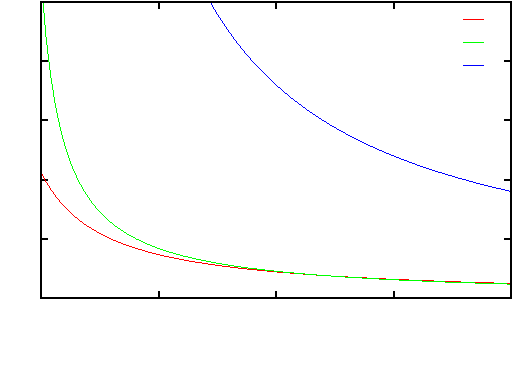
\includegraphics{nucleation_radius}}%
    \gplfronttext
  \end{picture}%
\endgroup
}\\
  \subfloat[]{\label{fig:cnt:criticalNumber}% GNUPLOT: LaTeX picture with Postscript
\begingroup
  \makeatletter
  \providecommand\color[2][]{%
    \GenericError{(gnuplot) \space\space\space\@spaces}{%
      Package color not loaded in conjunction with
      terminal option `colourtext'%
    }{See the gnuplot documentation for explanation.%
    }{Either use 'blacktext' in gnuplot or load the package
      color.sty in LaTeX.}%
    \renewcommand\color[2][]{}%
  }%
  \providecommand\includegraphics[2][]{%
    \GenericError{(gnuplot) \space\space\space\@spaces}{%
      Package graphicx or graphics not loaded%
    }{See the gnuplot documentation for explanation.%
    }{The gnuplot epslatex terminal needs graphicx.sty or graphics.sty.}%
    \renewcommand\includegraphics[2][]{}%
  }%
  \providecommand\rotatebox[2]{#2}%
  \@ifundefined{ifGPcolor}{%
    \newif\ifGPcolor
    \GPcolortrue
  }{}%
  \@ifundefined{ifGPblacktext}{%
    \newif\ifGPblacktext
    \GPblacktexttrue
  }{}%
  % define a \g@addto@macro without @ in the name:
  \let\gplgaddtomacro\g@addto@macro
  % define empty templates for all commands taking text:
  \gdef\gplbacktext{}%
  \gdef\gplfronttext{}%
  \makeatother
  \ifGPblacktext
    % no textcolor at all
    \def\colorrgb#1{}%
    \def\colorgray#1{}%
  \else
    % gray or color?
    \ifGPcolor
      \def\colorrgb#1{\color[rgb]{#1}}%
      \def\colorgray#1{\color[gray]{#1}}%
      \expandafter\def\csname LTw\endcsname{\color{white}}%
      \expandafter\def\csname LTb\endcsname{\color{black}}%
      \expandafter\def\csname LTa\endcsname{\color{black}}%
      \expandafter\def\csname LT0\endcsname{\color[rgb]{1,0,0}}%
      \expandafter\def\csname LT1\endcsname{\color[rgb]{0,1,0}}%
      \expandafter\def\csname LT2\endcsname{\color[rgb]{0,0,1}}%
      \expandafter\def\csname LT3\endcsname{\color[rgb]{1,0,1}}%
      \expandafter\def\csname LT4\endcsname{\color[rgb]{0,1,1}}%
      \expandafter\def\csname LT5\endcsname{\color[rgb]{1,1,0}}%
      \expandafter\def\csname LT6\endcsname{\color[rgb]{0,0,0}}%
      \expandafter\def\csname LT7\endcsname{\color[rgb]{1,0.3,0}}%
      \expandafter\def\csname LT8\endcsname{\color[rgb]{0.5,0.5,0.5}}%
    \else
      % gray
      \def\colorrgb#1{\color{black}}%
      \def\colorgray#1{\color[gray]{#1}}%
      \expandafter\def\csname LTw\endcsname{\color{white}}%
      \expandafter\def\csname LTb\endcsname{\color{black}}%
      \expandafter\def\csname LTa\endcsname{\color{black}}%
      \expandafter\def\csname LT0\endcsname{\color{black}}%
      \expandafter\def\csname LT1\endcsname{\color{black}}%
      \expandafter\def\csname LT2\endcsname{\color{black}}%
      \expandafter\def\csname LT3\endcsname{\color{black}}%
      \expandafter\def\csname LT4\endcsname{\color{black}}%
      \expandafter\def\csname LT5\endcsname{\color{black}}%
      \expandafter\def\csname LT6\endcsname{\color{black}}%
      \expandafter\def\csname LT7\endcsname{\color{black}}%
      \expandafter\def\csname LT8\endcsname{\color{black}}%
    \fi
  \fi
  \setlength{\unitlength}{0.0500bp}%
  \begin{picture}(5040.00,3528.00)%
    \gplgaddtomacro\gplbacktext{%
      \csname LTb\endcsname%
      \put(396,660){\makebox(0,0)[r]{\strut{} 0}}%
      \put(396,1371){\makebox(0,0)[r]{\strut{} 50}}%
      \put(396,2083){\makebox(0,0)[r]{\strut{} 100}}%
      \put(396,2794){\makebox(0,0)[r]{\strut{} 150}}%
      \put(396,3505){\makebox(0,0)[r]{\strut{} 200}}%
      \put(4908,440){\makebox(0,0){\strut{}-2}}%
      \put(3813,440){\makebox(0,0){\strut{}-1.5}}%
      \put(2718,440){\makebox(0,0){\strut{}-1}}%
      \put(1623,440){\makebox(0,0){\strut{}-0.5}}%
      \put(528,440){\makebox(0,0){\strut{} 0}}%
      \put(-374,2082){\rotatebox{90}{\makebox(0,0){\strut{}critical number of molecules}}}%
      \put(2718,110){\makebox(0,0){\strut{}negative pressure (MPa)}}%
    }%
    \gplgaddtomacro\gplfronttext{%
      \csname LTb\endcsname%
      \put(2112,1273){\makebox(0,0)[r]{\strut{}perfluorobutane}}%
      \csname LTb\endcsname%
      \put(2112,1053){\makebox(0,0)[r]{\strut{}perfluoropentane}}%
      \csname LTb\endcsname%
      \put(2112,833){\makebox(0,0)[r]{\strut{}water}}%
    }%
    \gplbacktext
    \put(0,0){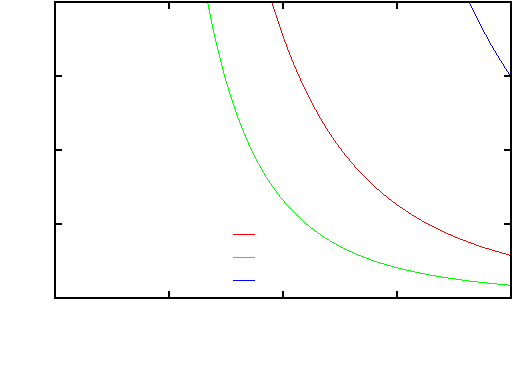
\includegraphics{nucleation_number}}%
    \gplfronttext
  \end{picture}%
\endgroup
}
\caption{
    Capillary predictions for the critical radius and critical number of molecules for a bubble as a function of the pressure at \unit{298}\kelvin.  
    The vapour is assumed to be an ideal gas, with the vapour pressure obtained by experimental fits to Antoine's equation.
    The coefficients for Antoine's equation are taken from National Institute of Standards Database\cite{NISTdata}
    (Note that the perfluorobutane data is used outside of its range of validity, see text).
  %  The other parameters are taken from the table. \tabref{nuc:parameters}.
  }
 \label{fig:cnt:nucleation_radius}
\end{figure}

We are now in a position to answer the first of our questions: the size of bubble expected to be cavitated.
This is because the critical radius provides  a lower bound for vapour bubbles in solution.
A bubble smaller than the critical radius will shrink even when  placed under tension,
and so is very unlikely to be observed.  


\figref{cnt:criticalRadius} uses equation \eqnref{LaplaceRelation} to plot the the critical radius as a function of pressure  for water, perfluoropentane and perfluorobutane
at  \unit{298}\kelvin.
The capillary approximation predicts that the critical radius is smaller for the perfluorocarbons than for water.
This is  encouraging, for it implies that type I nucleation is easier to induce for the perfluorocarbons than for water.
%However, the critical radii predicted are  somewhat large for our application.
%A \unit{20}\nano\metre-radius bubble represents more than 10\% of the radius of the oil-droplet.
%This undermines the assumption made that  neglects boundary between the oil droplet and the water.
%On the other hand, the capillary approximation is likely to be less severe.

At high pressures the critical radii of the two perfluorocarbons converge.
This is because the critical radius depends linearly on the surface tension (equation \eqnref{LaplaceRelation})
and the surface tensions are similar for perfluorocarbons.
Using a perfluorocarbon with a lower boiling point will enable smaller stable bubbles only at the more moderate  pressures where the vapour pressure plays a greater role.  
If higher pressures are used then the effect is negated.

%If therefore, Therefore, the gain in 
%At lower pressures the vapour pressure has a much greater role, which is higher in the case of perfluorobutane.
It should be noted that the vapour pressure used for perfluorobutane was extrapolated by \unit{29}\degreecelsius\  outside of its range of validity\cite{NISTdata}
 by use of Antoine's equation.
Since \unit{25}\degreecelsius\ is above the boiling point of perfluorobutane no  equilibrium vapour pressure can be defined.
However, since \unit{25}\degreecelsius\ is also well below the critical temperature, % (\tabref{:nuc:criticalTemps}), 
it is hoped that the predicted pressures within the (super-heated) bubble are still meaningful.
%The other parameters are taken from \tabref{nuc:parameters}.


In \figref{cnt:criticalNumber}  the predicted number of molecules contained within a critical bubble are plotted.
Again and as expected the number of perfluorocarbon molecules required to form a bubble are smaller than if the for water.
\Figref{cnt:criticalNumber} does, however, illustrate  the difficulty with the capillary approximation being used.
It is highly questionable that a bubble containing tens or even hundreds of molecules behaves like its thermodynamic bulk, with a constant density until the interface.
%The number of molecules is such that the thermodynamics starts to loose its meaning.


The capillary approximation predicts that a greater number of molecules are required to form a critical bubble for perfluorobutane than for perfluoropentane.
This is again due to the higher vapour pressure of  perfluorobutane.

%(A 20\nano\metre-diameter bubble {\em is} large to materialise by spontaneous fluctuation)
%the resulting bubble is not predicted to  contain too many molecules.
%The number of molecules within a critical bubble is perhaps more suggestive.
%This is the number of molecules that must join a bubble by fluctuation before it can grow.
%Again the number is far fewer for perfluoropentane than water.

%It is worthwhile estimating the number of molecules within the perfluoropentane bubble.
%For example, at a  negative pressure of \unit{1}\mega\pascal\ the critical radius
%of perfluoropentane is predicted to be \unit{8.7}\nano\metre\ at a vapour pressure of \unit{0.927}\ atmospheres.
%Assuming that the vapour behaves as an ideal gas, we find that the bubble contain approximately 60 molecules.




\section{Question 2: The vapourisation pressure of a perfluorocarbon droplet}\label{sec:nuc:vapourise}

There are two possible goals that may be set 
when imaging a bubble generated from a perfluorocarbon droplet:
\nlist{
 \item image the actual vaporisation event,
 \item image the resultant bubble after it has vaporised but before it redissolves.
}
%In this section we calculate the driving pressures that are required to achieve each of these goals.
Due to the stochastic nature of bubble nucleation, 
the pressures required to achieve these goals are best expressed in terms of pressures required
to achieve a given rate of nucleation,
the rate being such that observations are likely in the time frame of a given experiment.




\subsection{The rate required to image a vaporisation event}

For a nucleation event to be directly imaged
it must occur within the acoustical volume of the imaging pulse -
the volume in which the pressure is near its peak.
%
%To estimate the rate required to image a nucleation event
%we model the pulse as occupying a cylinder 
%The rate required to image a nucleation event can be estimated in terms of imaging pulse's wavelength, $\lambda$,
%and its acoustical volume, $V$.
The imaging volume is most simply approximated as a cylinder
and the pulse's principle wavelength, $\lambda$, makes a reasonable estimate for the diameter of a focused pulse.
If the pulse is $n$ cycles long then the acoustical volume, $V$, is given as so,
\begin{align}
  V \approx \frac{n  \pi \lambda^3 }{ 4}.
\end{align}
The duration of the pulse is $\tau_p=n\lambda/c$ and so it follows that the rate, $R$, at which the medium is sampled is 
\begin{align}
R \approx V/\tau_p = \frac{c\pi\lambda^2 }{4}
\label{eqn:nuc:rateOne}
\end{align}
The sampling rate of a \unit{15}\mega\hertz\ imaging pulse is therefore approximately
$\unit{10}\centi\metre\rpcubed\reciprocal\second$.
This gives the minimal rate of nucleation that would  be expected to be observed with a single a-line pulse.
It is only marginally greater than the limit of observation typically chosen in other nucleation applications: \unit{1}\centi\metre \rpcubed\reciprocal\second \cite{HongChul2005}.
For consistency with other applications, we therefore use this latter definition of  \unit{1}\centi\metre \rpcubed\reciprocal\second\
as the limit of what can be observed with ultrasound.
This corresponds to one nucleation event every 10 pulses.



\subsection{The rate required to image a generated bubble}

If only the bubble resulting from a nucleation event needs to be imaged, rather than the nucleation event itself, 
then the observable rate of nucleation is much lower.
This is because the bubble is potentially observable if the pulse passes within its lifetime 
and so it is the lifetime of the bubble, $\tau_b$, and not the duration of the acoustical pulse,
that defines the observable nucleation rate,
\begin{align}
R\approx V/\tau_b = \frac{n\pi\lambda^3}{4\tau_b}
\label{eqn:observable_rate_lifetime}
\end{align}
The value of $\tau_b$ will be evaluated when we consider the third of our questions in  \secref{nuc:lifetime}.
%To calculate the bubble's lifetime we assume that, at equilibrium, the bubble is smaller than its critical radius.
%Its lifetime is therefore defined by its rate of dissolution into the surrounding medium.
%This will be the usual case
%for although the bubble is greater than its critical radius when it is brought into existence,
%the driving wave is transient and in its absence the bubble will not normally continue to grow.



\subsection{The rate of bubble nucleation}


The rate of nucleation per unit volume is given by the Aarenhius equation, 
\begin{align}
J = J_0\exp \lr{-\frac{\Delta \Omega}{\kB T}},% = J_0 \exp\lr{- \frac{16\pi\gamma^3}{3\kB T\lr{p_v^\ast - p_L}^2}},
\label{eqn:nuc:J}
\end{align}
where $\Delta \Omega$ is the energy barrier to nucleation (in terms of the Grand Potential, $\Omega$),
$\kB$ is Boltzmann's constant, $T$ is the temperature
and $J_0$ is a rate  (per unit volume) obtained when $T\rightarrow \infty$ or when $\Delta G \rightarrow 0$.

The rate constant, $J_0$, for bubble nucleation is problematic.
The reason is that the definition of a very small bubble is not clear conceptually.
What is meant, for example, by a bubble of three molecules?
And how does one know when a new molecule has joined it?
Such uncertainties mean that arguments for $J_0$ very rapidly lose their precision.
%Molecules on the bubble edge will be close to the bulk medium and so the proximity of the mo
In contradistinction, the formation of a liquid droplet from a saturated vapour is clear conceptually:
a droplet of three molecules is easy to envisage, 
a cluster of just a few molecules is easier to define than a void.
Collision theory provides plausible arguments for the rate of droplet formation in a saturated vapour\cite{Katz1973}.
%
%A collection  because the proximity of the molecules in the droplet in comparison to the vapour is what defines the droplet.
%and when a new molecule becomes associated with the droplet  for the reason 
%Despite these differences
% and how it is to be distinguished from the bulk fluid is uncertain.
% boils down to it not being clear What is meant by the rate 
Be it on the grounds of reciprocity, or simply because a better alternative cannot be found,
the rate constant $J_o$ for bubble formation is usually taken to be the same 
as that for the formation of a liquid droplet from a saturated vapour\cite{Nyquist1995}.


Rather than repeat a spurious argument we prefer to estimate $J_0$ by dimensional analysis.
The result is the same as that used in the literature and is obtained at a fraction of the effort.
In addition, the estimate obtained here does not give the impression of greater accuracy than it deserves,
a danger ever present in kinematic derivations.

%Here we argue the calculation of $J_0$ on dimensional grounds.

At high temperatures, or when the energy barrier $\Delta G$ vanishes,
one would expect the detailed chemistry of the medium to become unimportant
with the liquid medium characterised as a collection of point particles of mass, $m$, and number density, $\rho_l$.
Likewise, a vapour bubble within the medium characterised by its number density, $\rho_v$, 
and surface tension, $\gamma$.
These properties are summarised in \tabref{nuc:dimensions} along with their dimensions.
%The variables that are deemed relevant are listed in \tabref{nuc:dimensional_vars} along with their dimensions.
There are five variables listed comprising of three dimensions: mass $[M]$, length $[L]$ and time $[t]$.
It is therefore possible to write down 2 dimensionless groups\cite{Goldreich1999}.


\ctable[cap=Nucleation dimensionless groups,
        caption=Dimensionless groups in the calculation of the nucleation rate constant,
        label=table:nuc:dimensions,
        pos=top,
        %width = 0.6\textwidth,
        left
       ]
       {llcrrc}
{
}{\FL
  &        & Parameter &Symbol & Dimension & 
  \ML
  &   Bubble      &  Rate of bubble growth  & $J_0$ & $[L]^3[t]^{-1}$ &
    \NN
    &  &  Vapour number density &$\rho_v$ &  $[M][L]^{-3}$    &
    \NN
    & &   Surface tension & $\gamma$ & $[M][T]^{-2}$    &
    \ML
    &Fluid  & Fluid number density & $\rho_l$  &  $[M][L]^{-3}$   &   
    \ML
    &Particle& Particle mass & $m$ & $[M]$ &
    \LL
  }

%The 5 variables split into variables that characterise the bubble
%\nlist{
%  \item the rate of bubble growth $J_0$
%  \item the vapour mass density, $m \rho_v$,
%  \item the surface tension, $\gamma$,
%}
%and a  variable that characterise the fluid
%\nlist{
%  \item the liquid mass density, $\rho_L$.
%}

To eliminate the temporal dependence $J_0$ must be squared 
and combined with surface tension.
The resulting $J^2/\gamma$ has the units $\lrsquare{M}^{-1}\lrsquare{L}^{-6}$.
% where the square brackets denote the units of mass and length, respectively.
These dimensions can be cancelled by using the particle mass  
and the square of a number density.
There is a choice as to which of the  number densities, $\rho_L$ and  $\rho_v$,  should be used.
Le Chatelier's principle advices that that denser liquids are more expensive (in terms of energy)
to separate, and that denser bubbles are less expensive to maintain.
One would expect, therefore, the rate $J_0$ to be proportional to $\rho_v$.
%The first non-dimensional group is therefore 
\begin{align}
  \Pi_1 &= \frac{J_0^2 m}{\gamma\rho_v^2}.
 \intertext{The second dimensionless group that can then be formed is then simply ratio of the densities,}
  \Pi_2 &= \frac{\rho_v}{\rho_L}.
\end{align}
Writing $\Pi_1$ as some function, $g$, of $\Pi_2$ we obtain,
\begin{align}
   J_0 = \rho_v \sqrt{\frac{\gamma}{m}} g\lr{\frac{\rho_v}{\rho_L}}.
\end{align}
The function $g$ is undetermined but for the reasons just argued
we anticipate $g$ to increase with $\rho_v$ and decrease with $\rho_L$.
%
%If the number density of the liquid is increased above equilibrium, then the excess chemical potential will be balanced if  molecules leave the fluid and enter the bubble.
%The nucleation rate should therefore increase with $\rho_L$.
%Conversely,  the nucleation rate should  decrease with an increased vapour density, $\rho_v$.
The simplest such relationship %between rate and density 
is a linear one
and so we guess $g(x) \propto x$.
If the constant of proportionality is assumed to be approximately unity, then 
for  bubble nucleation we have
%
%This is the conventional form for the pre-exponential factor in bubble nucleation.
%
%
%The result of the collision theory argument of Katz\cite{Katz1992} is that
%%
%Due to the uncertain nature of the derivation
%Conceptually, however, bubble formation and droplet condensation are very different.
%
%However, conceptually the models are 
%The rate for a liquid droplet may be derived kinematically by  collision theory argument used to find the rate of formation of a liquid droplet from a saturated vapour.
%The adaptation is problematic, however.
%When modeIn the liquid droplet model the  droplet is modelled as a cluster of  molecules bound together, 
%and the rate   at which,  say, a fourth molecule condenses onto a cluster of three molecules is clear conceptually.
%What is meant by a `bubble of three molecules', and how it is to be distinguished from the bulk fluid is uncertain.
%Nevertheless, we use the results of such a derivation\cite{Katz1992}. % (which we provide in \appref{CNT} for completeness), 
%
%Nevertheless, we carry to calculate the rate of nucleation,
%so at least to have a benchmark with which to compare the density functional method we use in \secref{nuc:DFT}.
%
\begin{align}
  J_0 \approx \frac{\rho_v^2}{\rho_l}\sqrt{\frac{\gamma}{m}},
\end{align}
This is identical to the result of the collision theory argument of Katz\cite{Katz1992}.
%where $m$ is the mass of the particle, $rho_v$ and $\rho_l$ are the densities of the vapour and bubble respectively,
%and $\gamma$ is \todo{What is gamma}.
For water $J_0\approx 10^{34}\centi\metre \rpcubed \reciprocal\second$ and for perfluoropentane $J_0\approx 10^{32}\centi\metre \rpcubed \reciprocal\second$. 

%To complete \eqnref{observable_rate_lifetime} it is necessary to calculate the lifetime of a bubble.
%A generated bubble can either redissolve or grow and form a large bubble that will 
%float to the surface of the experimental chamber.
%Here we assume that the generated bubble is below it critical radius, 
%and we evaluate the lifetime of the bubble prior to it redissolving.



\subsection{Results}

\begin{figure}
 \centering
  \subfloat[Nucleation rates for water, \pfp\ and \pfb\ at 25\degreecelsius.]{\label{fig:cnt:rate:chem}% GNUPLOT: LaTeX picture with Postscript
\begingroup
  \makeatletter
  \providecommand\color[2][]{%
    \GenericError{(gnuplot) \space\space\space\@spaces}{%
      Package color not loaded in conjunction with
      terminal option `colourtext'%
    }{See the gnuplot documentation for explanation.%
    }{Either use 'blacktext' in gnuplot or load the package
      color.sty in LaTeX.}%
    \renewcommand\color[2][]{}%
  }%
  \providecommand\includegraphics[2][]{%
    \GenericError{(gnuplot) \space\space\space\@spaces}{%
      Package graphicx or graphics not loaded%
    }{See the gnuplot documentation for explanation.%
    }{The gnuplot epslatex terminal needs graphicx.sty or graphics.sty.}%
    \renewcommand\includegraphics[2][]{}%
  }%
  \providecommand\rotatebox[2]{#2}%
  \@ifundefined{ifGPcolor}{%
    \newif\ifGPcolor
    \GPcolortrue
  }{}%
  \@ifundefined{ifGPblacktext}{%
    \newif\ifGPblacktext
    \GPblacktexttrue
  }{}%
  % define a \g@addto@macro without @ in the name:
  \let\gplgaddtomacro\g@addto@macro
  % define empty templates for all commands taking text:
  \gdef\gplbacktext{}%
  \gdef\gplfronttext{}%
  \makeatother
  \ifGPblacktext
    % no textcolor at all
    \def\colorrgb#1{}%
    \def\colorgray#1{}%
  \else
    % gray or color?
    \ifGPcolor
      \def\colorrgb#1{\color[rgb]{#1}}%
      \def\colorgray#1{\color[gray]{#1}}%
      \expandafter\def\csname LTw\endcsname{\color{white}}%
      \expandafter\def\csname LTb\endcsname{\color{black}}%
      \expandafter\def\csname LTa\endcsname{\color{black}}%
      \expandafter\def\csname LT0\endcsname{\color[rgb]{1,0,0}}%
      \expandafter\def\csname LT1\endcsname{\color[rgb]{0,1,0}}%
      \expandafter\def\csname LT2\endcsname{\color[rgb]{0,0,1}}%
      \expandafter\def\csname LT3\endcsname{\color[rgb]{1,0,1}}%
      \expandafter\def\csname LT4\endcsname{\color[rgb]{0,1,1}}%
      \expandafter\def\csname LT5\endcsname{\color[rgb]{1,1,0}}%
      \expandafter\def\csname LT6\endcsname{\color[rgb]{0,0,0}}%
      \expandafter\def\csname LT7\endcsname{\color[rgb]{1,0.3,0}}%
      \expandafter\def\csname LT8\endcsname{\color[rgb]{0.5,0.5,0.5}}%
    \else
      % gray
      \def\colorrgb#1{\color{black}}%
      \def\colorgray#1{\color[gray]{#1}}%
      \expandafter\def\csname LTw\endcsname{\color{white}}%
      \expandafter\def\csname LTb\endcsname{\color{black}}%
      \expandafter\def\csname LTa\endcsname{\color{black}}%
      \expandafter\def\csname LT0\endcsname{\color{black}}%
      \expandafter\def\csname LT1\endcsname{\color{black}}%
      \expandafter\def\csname LT2\endcsname{\color{black}}%
      \expandafter\def\csname LT3\endcsname{\color{black}}%
      \expandafter\def\csname LT4\endcsname{\color{black}}%
      \expandafter\def\csname LT5\endcsname{\color{black}}%
      \expandafter\def\csname LT6\endcsname{\color{black}}%
      \expandafter\def\csname LT7\endcsname{\color{black}}%
      \expandafter\def\csname LT8\endcsname{\color{black}}%
    \fi
  \fi
  \setlength{\unitlength}{0.0500bp}%
  \begin{picture}(5040.00,3528.00)%
    \gplgaddtomacro\gplbacktext{%
      \csname LTb\endcsname%
      \put(1188,660){\makebox(0,0)[r]{\strut{}$10^{-40}$}}%
      \put(1188,976){\makebox(0,0)[r]{\strut{}$10^{-30}$}}%
      \put(1188,1292){\makebox(0,0)[r]{\strut{}$10^{-20}$}}%
      \put(1188,1608){\makebox(0,0)[r]{\strut{}$10^{-10}$}}%
      \put(1188,1924){\makebox(0,0)[r]{\strut{}$10^{0}$}}%
      \put(1188,2241){\makebox(0,0)[r]{\strut{}$10^{10}$}}%
      \put(1188,2557){\makebox(0,0)[r]{\strut{}$10^{20}$}}%
      \put(1188,2873){\makebox(0,0)[r]{\strut{}$10^{30}$}}%
      \put(1188,3189){\makebox(0,0)[r]{\strut{}$10^{40}$}}%
      \put(1188,3505){\makebox(0,0)[r]{\strut{}$10^{50}$}}%
      \put(4907,440){\makebox(0,0){\strut{} 1}}%
      \put(3348,440){\makebox(0,0){\strut{} 10}}%
      \put(1789,440){\makebox(0,0){\strut{} 100}}%
      \put(286,2082){\rotatebox{-270}{\makebox(0,0){\strut{}nucleation rate ($\centi\meter^{-3}\second^{-1}$)}}}%
      \put(3113,110){\makebox(0,0){\strut{}negative pressure (MPa)}}%
    }%
    \gplgaddtomacro\gplfronttext{%
      \csname LTb\endcsname%
      \put(4316,3332){\makebox(0,0)[r]{\strut{}perfluorobutane}}%
      \csname LTb\endcsname%
      \put(4316,3112){\makebox(0,0)[r]{\strut{}perfluoropentane}}%
      \csname LTb\endcsname%
      \put(4316,2892){\makebox(0,0)[r]{\strut{}water}}%
    }%
    \gplbacktext
    \put(0,0){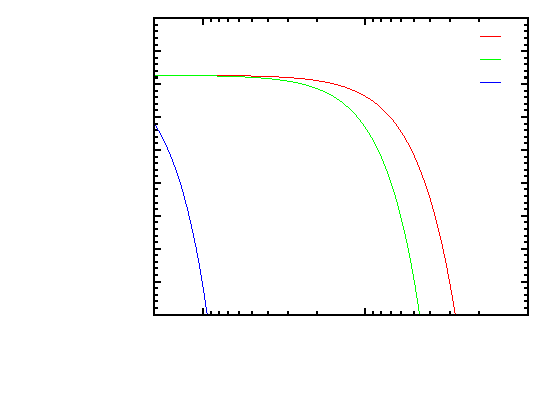
\includegraphics{c2_cnt_nucleation_rate2}}%
    \gplfronttext
  \end{picture}%
\endgroup
}\\
  \subfloat[Nucleation rates for  \pfp\ at different temperatures.]{\label{fig:cnt:rate:temp}% GNUPLOT: LaTeX picture with Postscript
\begingroup
  \makeatletter
  \providecommand\color[2][]{%
    \GenericError{(gnuplot) \space\space\space\@spaces}{%
      Package color not loaded in conjunction with
      terminal option `colourtext'%
    }{See the gnuplot documentation for explanation.%
    }{Either use 'blacktext' in gnuplot or load the package
      color.sty in LaTeX.}%
    \renewcommand\color[2][]{}%
  }%
  \providecommand\includegraphics[2][]{%
    \GenericError{(gnuplot) \space\space\space\@spaces}{%
      Package graphicx or graphics not loaded%
    }{See the gnuplot documentation for explanation.%
    }{The gnuplot epslatex terminal needs graphicx.sty or graphics.sty.}%
    \renewcommand\includegraphics[2][]{}%
  }%
  \providecommand\rotatebox[2]{#2}%
  \@ifundefined{ifGPcolor}{%
    \newif\ifGPcolor
    \GPcolortrue
  }{}%
  \@ifundefined{ifGPblacktext}{%
    \newif\ifGPblacktext
    \GPblacktexttrue
  }{}%
  % define a \g@addto@macro without @ in the name:
  \let\gplgaddtomacro\g@addto@macro
  % define empty templates for all commands taking text:
  \gdef\gplbacktext{}%
  \gdef\gplfronttext{}%
  \makeatother
  \ifGPblacktext
    % no textcolor at all
    \def\colorrgb#1{}%
    \def\colorgray#1{}%
  \else
    % gray or color?
    \ifGPcolor
      \def\colorrgb#1{\color[rgb]{#1}}%
      \def\colorgray#1{\color[gray]{#1}}%
      \expandafter\def\csname LTw\endcsname{\color{white}}%
      \expandafter\def\csname LTb\endcsname{\color{black}}%
      \expandafter\def\csname LTa\endcsname{\color{black}}%
      \expandafter\def\csname LT0\endcsname{\color[rgb]{1,0,0}}%
      \expandafter\def\csname LT1\endcsname{\color[rgb]{0,1,0}}%
      \expandafter\def\csname LT2\endcsname{\color[rgb]{0,0,1}}%
      \expandafter\def\csname LT3\endcsname{\color[rgb]{1,0,1}}%
      \expandafter\def\csname LT4\endcsname{\color[rgb]{0,1,1}}%
      \expandafter\def\csname LT5\endcsname{\color[rgb]{1,1,0}}%
      \expandafter\def\csname LT6\endcsname{\color[rgb]{0,0,0}}%
      \expandafter\def\csname LT7\endcsname{\color[rgb]{1,0.3,0}}%
      \expandafter\def\csname LT8\endcsname{\color[rgb]{0.5,0.5,0.5}}%
    \else
      % gray
      \def\colorrgb#1{\color{black}}%
      \def\colorgray#1{\color[gray]{#1}}%
      \expandafter\def\csname LTw\endcsname{\color{white}}%
      \expandafter\def\csname LTb\endcsname{\color{black}}%
      \expandafter\def\csname LTa\endcsname{\color{black}}%
      \expandafter\def\csname LT0\endcsname{\color{black}}%
      \expandafter\def\csname LT1\endcsname{\color{black}}%
      \expandafter\def\csname LT2\endcsname{\color{black}}%
      \expandafter\def\csname LT3\endcsname{\color{black}}%
      \expandafter\def\csname LT4\endcsname{\color{black}}%
      \expandafter\def\csname LT5\endcsname{\color{black}}%
      \expandafter\def\csname LT6\endcsname{\color{black}}%
      \expandafter\def\csname LT7\endcsname{\color{black}}%
      \expandafter\def\csname LT8\endcsname{\color{black}}%
    \fi
  \fi
  \setlength{\unitlength}{0.0500bp}%
  \begin{picture}(5040.00,3528.00)%
    \gplgaddtomacro\gplbacktext{%
      \csname LTb\endcsname%
      \put(1188,660){\makebox(0,0)[r]{\strut{}$10^{-40}$}}%
      \put(1188,1134){\makebox(0,0)[r]{\strut{}$10^{-30}$}}%
      \put(1188,1608){\makebox(0,0)[r]{\strut{}$10^{-20}$}}%
      \put(1188,2083){\makebox(0,0)[r]{\strut{}$10^{-10}$}}%
      \put(1188,2557){\makebox(0,0)[r]{\strut{}$10^{0}$}}%
      \put(1188,3031){\makebox(0,0)[r]{\strut{}$10^{10}$}}%
      \put(1188,3505){\makebox(0,0)[r]{\strut{}$10^{20}$}}%
      \put(4907,440){\makebox(0,0){\strut{} 1}}%
      \put(4508,440){\makebox(0,0){\strut{} 2}}%
      \put(4110,440){\makebox(0,0){\strut{} 3}}%
      \put(3711,440){\makebox(0,0){\strut{} 4}}%
      \put(3313,440){\makebox(0,0){\strut{} 5}}%
      \put(2914,440){\makebox(0,0){\strut{} 6}}%
      \put(2516,440){\makebox(0,0){\strut{} 7}}%
      \put(2117,440){\makebox(0,0){\strut{} 8}}%
      \put(1719,440){\makebox(0,0){\strut{} 9}}%
      \put(1320,440){\makebox(0,0){\strut{} 10}}%
      \put(286,2082){\rotatebox{-270}{\makebox(0,0){\strut{}nucleation rate ($\centi\meter^{-3}\second^{-1}$)}}}%
      \put(3113,110){\makebox(0,0){\strut{}negative pressure (MPa)}}%
    }%
    \gplgaddtomacro\gplfronttext{%
      \csname LTb\endcsname%
      \put(4316,3332){\makebox(0,0)[r]{\strut{}273 K}}%
      \csname LTb\endcsname%
      \put(4316,3112){\makebox(0,0)[r]{\strut{}283 K}}%
      \csname LTb\endcsname%
      \put(4316,2892){\makebox(0,0)[r]{\strut{}293 K}}%
      \csname LTb\endcsname%
      \put(4316,2672){\makebox(0,0)[r]{\strut{}303 K}}%
    }%
    \gplbacktext
    \put(0,0){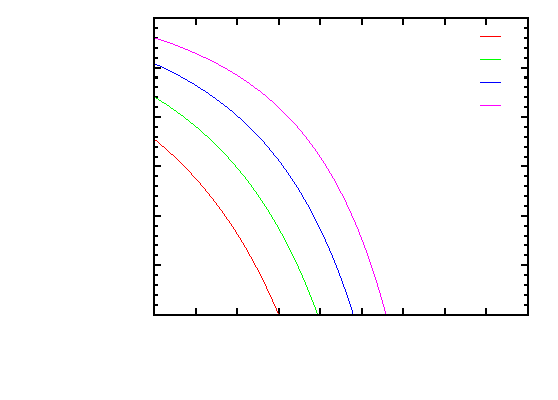
\includegraphics{c2_cnt_nucleation_rate_temp}}%
    \gplfronttext
  \end{picture}%
\endgroup
}
  \caption{
    Nucleation rates evaluated from equation \eqnref{nuc:J}.  The NIST Chemistry WebBook\cite{NISTdata} being used as the source for the required  experimental constants.
  }
 \label{fig:cnt:rate}
\end{figure}


The nucleation rates calculated with the capillary approximation are plotted in \figref{cnt:rate}.
In \figref{cnt:rate:chem} the rates   for \pfb,  perfluoropentane and water are plotted.
As expected from the plot of critical radii, \figref{cnt:criticalRadius}, 
high rates of nucleation are obtained at lower pressures with the perflurocarbons than for water,
with \pfb\ being more easily cavitated than \pfp.
This is encouraging, for increasing the rate of type I nucleation was the motivation for considering the perfluorocarbons.


However, the pressures given by \figref{cnt:rate}  to observe type I nucleation are high for diagnostic ultrasound.
\figref{cnt:rate:chem} suggests that  \pfb, even when in a supersaturated state,
will  require a negative pressure in the region of \unit{4}\mega\pascal\ to be observable. 
Such pressures are used in medical ultrasound, but require the specially engineered transducers of HIFU.
To observe \pfp\ the negative pressure will need to be in the region of \unit{8}\mega\pascal,
and while \figref{cnt:rate:temp} shows that the temperature is influential, 
it is not so influential as to shift the pressures back to those obtainable with diagnostic transducers.
These pressures are of the same order of magnitude as the experimental values of Schad\cite{Schad2009}.




\section{Question 3: The lifetime of a vapour bubble}\label{sec:nuc:lifetime}


\begin{figure}
  \subfloat[Dissolution of a \unit{1}\micro\metre\ air bubble when $\zeta=0$]{ \label{fig:nuc:dissolve_time_lum}% GNUPLOT: LaTeX picture with Postscript
\begingroup
  \makeatletter
  \providecommand\color[2][]{%
    \GenericError{(gnuplot) \space\space\space\@spaces}{%
      Package color not loaded in conjunction with
      terminal option `colourtext'%
    }{See the gnuplot documentation for explanation.%
    }{Either use 'blacktext' in gnuplot or load the package
      color.sty in LaTeX.}%
    \renewcommand\color[2][]{}%
  }%
  \providecommand\includegraphics[2][]{%
    \GenericError{(gnuplot) \space\space\space\@spaces}{%
      Package graphicx or graphics not loaded%
    }{See the gnuplot documentation for explanation.%
    }{The gnuplot epslatex terminal needs graphicx.sty or graphics.sty.}%
    \renewcommand\includegraphics[2][]{}%
  }%
  \providecommand\rotatebox[2]{#2}%
  \@ifundefined{ifGPcolor}{%
    \newif\ifGPcolor
    \GPcolorfalse
  }{}%
  \@ifundefined{ifGPblacktext}{%
    \newif\ifGPblacktext
    \GPblacktexttrue
  }{}%
  % define a \g@addto@macro without @ in the name:
  \let\gplgaddtomacro\g@addto@macro
  % define empty templates for all commands taking text:
  \gdef\gplbacktext{}%
  \gdef\gplfronttext{}%
  \makeatother
  \ifGPblacktext
    % no textcolor at all
    \def\colorrgb#1{}%
    \def\colorgray#1{}%
  \else
    % gray or color?
    \ifGPcolor
      \def\colorrgb#1{\color[rgb]{#1}}%
      \def\colorgray#1{\color[gray]{#1}}%
      \expandafter\def\csname LTw\endcsname{\color{white}}%
      \expandafter\def\csname LTb\endcsname{\color{black}}%
      \expandafter\def\csname LTa\endcsname{\color{black}}%
      \expandafter\def\csname LT0\endcsname{\color[rgb]{1,0,0}}%
      \expandafter\def\csname LT1\endcsname{\color[rgb]{0,1,0}}%
      \expandafter\def\csname LT2\endcsname{\color[rgb]{0,0,1}}%
      \expandafter\def\csname LT3\endcsname{\color[rgb]{1,0,1}}%
      \expandafter\def\csname LT4\endcsname{\color[rgb]{0,1,1}}%
      \expandafter\def\csname LT5\endcsname{\color[rgb]{1,1,0}}%
      \expandafter\def\csname LT6\endcsname{\color[rgb]{0,0,0}}%
      \expandafter\def\csname LT7\endcsname{\color[rgb]{1,0.3,0}}%
      \expandafter\def\csname LT8\endcsname{\color[rgb]{0.5,0.5,0.5}}%
    \else
      % gray
      \def\colorrgb#1{\color{black}}%
      \def\colorgray#1{\color[gray]{#1}}%
      \expandafter\def\csname LTw\endcsname{\color{white}}%
      \expandafter\def\csname LTb\endcsname{\color{black}}%
      \expandafter\def\csname LTa\endcsname{\color{black}}%
      \expandafter\def\csname LT0\endcsname{\color{black}}%
      \expandafter\def\csname LT1\endcsname{\color{black}}%
      \expandafter\def\csname LT2\endcsname{\color{black}}%
      \expandafter\def\csname LT3\endcsname{\color{black}}%
      \expandafter\def\csname LT4\endcsname{\color{black}}%
      \expandafter\def\csname LT5\endcsname{\color{black}}%
      \expandafter\def\csname LT6\endcsname{\color{black}}%
      \expandafter\def\csname LT7\endcsname{\color{black}}%
      \expandafter\def\csname LT8\endcsname{\color{black}}%
    \fi
  \fi
  \setlength{\unitlength}{0.0500bp}%
  \begin{picture}(4320.00,3024.00)%
    \gplgaddtomacro\gplbacktext{%
      \csname LTb\endcsname%
      \put(946,704){\makebox(0,0)[r]{\strut{} 0}}%
      \put(946,910){\makebox(0,0)[r]{\strut{} 0.1}}%
      \put(946,1115){\makebox(0,0)[r]{\strut{} 0.2}}%
      \put(946,1321){\makebox(0,0)[r]{\strut{} 0.3}}%
      \put(946,1526){\makebox(0,0)[r]{\strut{} 0.4}}%
      \put(946,1732){\makebox(0,0)[r]{\strut{} 0.5}}%
      \put(946,1937){\makebox(0,0)[r]{\strut{} 0.6}}%
      \put(946,2143){\makebox(0,0)[r]{\strut{} 0.7}}%
      \put(946,2348){\makebox(0,0)[r]{\strut{} 0.8}}%
      \put(946,2554){\makebox(0,0)[r]{\strut{} 0.9}}%
      \put(946,2759){\makebox(0,0)[r]{\strut{} 1}}%
      \put(1078,484){\makebox(0,0){\strut{} 0}}%
      \put(1434,484){\makebox(0,0){\strut{} 2}}%
      \put(1789,484){\makebox(0,0){\strut{} 4}}%
      \put(2145,484){\makebox(0,0){\strut{} 6}}%
      \put(2501,484){\makebox(0,0){\strut{} 8}}%
      \put(2856,484){\makebox(0,0){\strut{} 10}}%
      \put(3212,484){\makebox(0,0){\strut{} 12}}%
      \put(3567,484){\makebox(0,0){\strut{} 14}}%
      \put(3923,484){\makebox(0,0){\strut{} 16}}%
      \put(176,1731){\rotatebox{-270}{\makebox(0,0){\strut{}radius ($\mu$m)}}}%
      \put(2500,154){\makebox(0,0){\strut{}time (ms)}}%
    }%
    \gplgaddtomacro\gplfronttext{%
    }%
    \gplbacktext
    \put(0,0){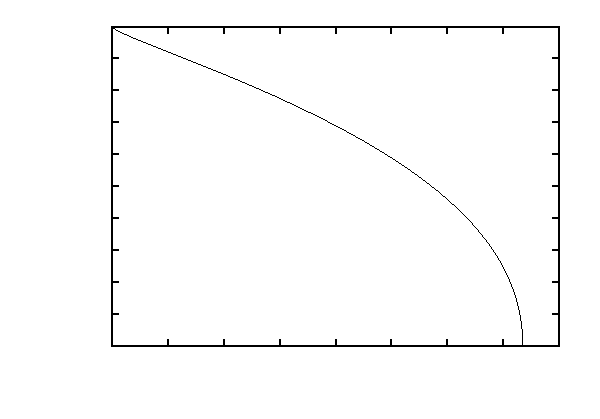
\includegraphics{chNucDissolveTimeLum}}%
    \gplfronttext
  \end{picture}%
\endgroup
}
  \subfloat[Dissolution time as a function of radius]{ \label{fig:nuc:dissolve_time}% GNUPLOT: LaTeX picture with Postscript
\begingroup
  \makeatletter
  \providecommand\color[2][]{%
    \GenericError{(gnuplot) \space\space\space\@spaces}{%
      Package color not loaded in conjunction with
      terminal option `colourtext'%
    }{See the gnuplot documentation for explanation.%
    }{Either use 'blacktext' in gnuplot or load the package
      color.sty in LaTeX.}%
    \renewcommand\color[2][]{}%
  }%
  \providecommand\includegraphics[2][]{%
    \GenericError{(gnuplot) \space\space\space\@spaces}{%
      Package graphicx or graphics not loaded%
    }{See the gnuplot documentation for explanation.%
    }{The gnuplot epslatex terminal needs graphicx.sty or graphics.sty.}%
    \renewcommand\includegraphics[2][]{}%
  }%
  \providecommand\rotatebox[2]{#2}%
  \@ifundefined{ifGPcolor}{%
    \newif\ifGPcolor
    \GPcolorfalse
  }{}%
  \@ifundefined{ifGPblacktext}{%
    \newif\ifGPblacktext
    \GPblacktexttrue
  }{}%
  % define a \g@addto@macro without @ in the name:
  \let\gplgaddtomacro\g@addto@macro
  % define empty templates for all commands taking text:
  \gdef\gplbacktext{}%
  \gdef\gplfronttext{}%
  \makeatother
  \ifGPblacktext
    % no textcolor at all
    \def\colorrgb#1{}%
    \def\colorgray#1{}%
  \else
    % gray or color?
    \ifGPcolor
      \def\colorrgb#1{\color[rgb]{#1}}%
      \def\colorgray#1{\color[gray]{#1}}%
      \expandafter\def\csname LTw\endcsname{\color{white}}%
      \expandafter\def\csname LTb\endcsname{\color{black}}%
      \expandafter\def\csname LTa\endcsname{\color{black}}%
      \expandafter\def\csname LT0\endcsname{\color[rgb]{1,0,0}}%
      \expandafter\def\csname LT1\endcsname{\color[rgb]{0,1,0}}%
      \expandafter\def\csname LT2\endcsname{\color[rgb]{0,0,1}}%
      \expandafter\def\csname LT3\endcsname{\color[rgb]{1,0,1}}%
      \expandafter\def\csname LT4\endcsname{\color[rgb]{0,1,1}}%
      \expandafter\def\csname LT5\endcsname{\color[rgb]{1,1,0}}%
      \expandafter\def\csname LT6\endcsname{\color[rgb]{0,0,0}}%
      \expandafter\def\csname LT7\endcsname{\color[rgb]{1,0.3,0}}%
      \expandafter\def\csname LT8\endcsname{\color[rgb]{0.5,0.5,0.5}}%
    \else
      % gray
      \def\colorrgb#1{\color{black}}%
      \def\colorgray#1{\color[gray]{#1}}%
      \expandafter\def\csname LTw\endcsname{\color{white}}%
      \expandafter\def\csname LTb\endcsname{\color{black}}%
      \expandafter\def\csname LTa\endcsname{\color{black}}%
      \expandafter\def\csname LT0\endcsname{\color{black}}%
      \expandafter\def\csname LT1\endcsname{\color{black}}%
      \expandafter\def\csname LT2\endcsname{\color{black}}%
      \expandafter\def\csname LT3\endcsname{\color{black}}%
      \expandafter\def\csname LT4\endcsname{\color{black}}%
      \expandafter\def\csname LT5\endcsname{\color{black}}%
      \expandafter\def\csname LT6\endcsname{\color{black}}%
      \expandafter\def\csname LT7\endcsname{\color{black}}%
      \expandafter\def\csname LT8\endcsname{\color{black}}%
    \fi
  \fi
  \setlength{\unitlength}{0.0500bp}%
  \begin{picture}(4320.00,3024.00)%
    \gplgaddtomacro\gplbacktext{%
      \csname LTb\endcsname%
      \put(946,704){\makebox(0,0)[r]{\strut{}$10^{-2}$}}%
      \put(946,1115){\makebox(0,0)[r]{\strut{}$10^{-1}$}}%
      \put(946,1526){\makebox(0,0)[r]{\strut{}$10^{0}$}}%
      \put(946,1937){\makebox(0,0)[r]{\strut{}$10^{1}$}}%
      \put(946,2348){\makebox(0,0)[r]{\strut{}$10^{2}$}}%
      \put(946,2759){\makebox(0,0)[r]{\strut{}$10^{3}$}}%
      \put(1078,484){\makebox(0,0){\strut{}$10^{-2}$}}%
      \put(2026,484){\makebox(0,0){\strut{}$10^{-1}$}}%
      \put(2975,484){\makebox(0,0){\strut{}$10^{0}$}}%
      \put(3923,484){\makebox(0,0){\strut{}$10^{1}$}}%
      \put(176,1731){\rotatebox{-270}{\makebox(0,0){\strut{}dissolution time (ms)}}}%
      \put(2500,154){\makebox(0,0){\strut{}initial radius ($\mu$m)}}%
    }%
    \gplgaddtomacro\gplfronttext{%
      \csname LTb\endcsname%
      \put(2662,2586){\makebox(0,0)[r]{\strut{}saturated}}%
      \csname LTb\endcsname%
      \put(2662,2366){\makebox(0,0)[r]{\strut{}unsaturated}}%
    }%
    \gplbacktext
    \put(0,0){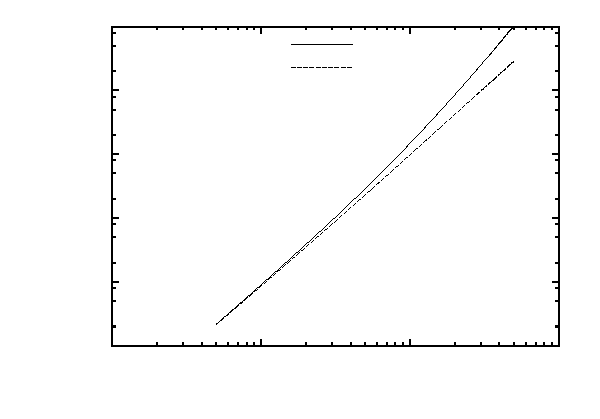
\includegraphics{chNucDissolveTime}}%
    \gplfronttext
  \end{picture}%
\endgroup
}
  \caption{ Dissolve times of air bubbles.  The experimental quantities used in the model are given in \tabref{nuc:dissolveVars}.}
\end{figure}

\begin{figure}
  \subfloat[Dissolution of a \unit{1}\micro\metre\ \pfp\ bubble when $\zeta=0$]{\label{fig:nuc:dissolve_time_lumPFP}% GNUPLOT: LaTeX picture with Postscript
\begingroup
  \makeatletter
  \providecommand\color[2][]{%
    \GenericError{(gnuplot) \space\space\space\@spaces}{%
      Package color not loaded in conjunction with
      terminal option `colourtext'%
    }{See the gnuplot documentation for explanation.%
    }{Either use 'blacktext' in gnuplot or load the package
      color.sty in LaTeX.}%
    \renewcommand\color[2][]{}%
  }%
  \providecommand\includegraphics[2][]{%
    \GenericError{(gnuplot) \space\space\space\@spaces}{%
      Package graphicx or graphics not loaded%
    }{See the gnuplot documentation for explanation.%
    }{The gnuplot epslatex terminal needs graphicx.sty or graphics.sty.}%
    \renewcommand\includegraphics[2][]{}%
  }%
  \providecommand\rotatebox[2]{#2}%
  \@ifundefined{ifGPcolor}{%
    \newif\ifGPcolor
    \GPcolorfalse
  }{}%
  \@ifundefined{ifGPblacktext}{%
    \newif\ifGPblacktext
    \GPblacktexttrue
  }{}%
  % define a \g@addto@macro without @ in the name:
  \let\gplgaddtomacro\g@addto@macro
  % define empty templates for all commands taking text:
  \gdef\gplbacktext{}%
  \gdef\gplfronttext{}%
  \makeatother
  \ifGPblacktext
    % no textcolor at all
    \def\colorrgb#1{}%
    \def\colorgray#1{}%
  \else
    % gray or color?
    \ifGPcolor
      \def\colorrgb#1{\color[rgb]{#1}}%
      \def\colorgray#1{\color[gray]{#1}}%
      \expandafter\def\csname LTw\endcsname{\color{white}}%
      \expandafter\def\csname LTb\endcsname{\color{black}}%
      \expandafter\def\csname LTa\endcsname{\color{black}}%
      \expandafter\def\csname LT0\endcsname{\color[rgb]{1,0,0}}%
      \expandafter\def\csname LT1\endcsname{\color[rgb]{0,1,0}}%
      \expandafter\def\csname LT2\endcsname{\color[rgb]{0,0,1}}%
      \expandafter\def\csname LT3\endcsname{\color[rgb]{1,0,1}}%
      \expandafter\def\csname LT4\endcsname{\color[rgb]{0,1,1}}%
      \expandafter\def\csname LT5\endcsname{\color[rgb]{1,1,0}}%
      \expandafter\def\csname LT6\endcsname{\color[rgb]{0,0,0}}%
      \expandafter\def\csname LT7\endcsname{\color[rgb]{1,0.3,0}}%
      \expandafter\def\csname LT8\endcsname{\color[rgb]{0.5,0.5,0.5}}%
    \else
      % gray
      \def\colorrgb#1{\color{black}}%
      \def\colorgray#1{\color[gray]{#1}}%
      \expandafter\def\csname LTw\endcsname{\color{white}}%
      \expandafter\def\csname LTb\endcsname{\color{black}}%
      \expandafter\def\csname LTa\endcsname{\color{black}}%
      \expandafter\def\csname LT0\endcsname{\color{black}}%
      \expandafter\def\csname LT1\endcsname{\color{black}}%
      \expandafter\def\csname LT2\endcsname{\color{black}}%
      \expandafter\def\csname LT3\endcsname{\color{black}}%
      \expandafter\def\csname LT4\endcsname{\color{black}}%
      \expandafter\def\csname LT5\endcsname{\color{black}}%
      \expandafter\def\csname LT6\endcsname{\color{black}}%
      \expandafter\def\csname LT7\endcsname{\color{black}}%
      \expandafter\def\csname LT8\endcsname{\color{black}}%
    \fi
  \fi
  \setlength{\unitlength}{0.0500bp}%
  \begin{picture}(5760.00,4032.00)%
    \gplgaddtomacro\gplbacktext{%
      \csname LTb\endcsname%
      \put(946,704){\makebox(0,0)[r]{\strut{} 0}}%
      \put(946,1010){\makebox(0,0)[r]{\strut{} 0.1}}%
      \put(946,1317){\makebox(0,0)[r]{\strut{} 0.2}}%
      \put(946,1623){\makebox(0,0)[r]{\strut{} 0.3}}%
      \put(946,1929){\makebox(0,0)[r]{\strut{} 0.4}}%
      \put(946,2236){\makebox(0,0)[r]{\strut{} 0.5}}%
      \put(946,2542){\makebox(0,0)[r]{\strut{} 0.6}}%
      \put(946,2848){\makebox(0,0)[r]{\strut{} 0.7}}%
      \put(946,3154){\makebox(0,0)[r]{\strut{} 0.8}}%
      \put(946,3461){\makebox(0,0)[r]{\strut{} 0.9}}%
      \put(946,3767){\makebox(0,0)[r]{\strut{} 1}}%
      \put(1078,484){\makebox(0,0){\strut{} 0}}%
      \put(1792,484){\makebox(0,0){\strut{} 20}}%
      \put(2506,484){\makebox(0,0){\strut{} 40}}%
      \put(3221,484){\makebox(0,0){\strut{} 60}}%
      \put(3935,484){\makebox(0,0){\strut{} 80}}%
      \put(4649,484){\makebox(0,0){\strut{} 100}}%
      \put(5363,484){\makebox(0,0){\strut{} 120}}%
      \put(176,2235){\rotatebox{-270}{\makebox(0,0){\strut{}radius ($\mu$m)}}}%
      \put(3220,154){\makebox(0,0){\strut{}time (s)}}%
    }%
    \gplgaddtomacro\gplfronttext{%
    }%
    \gplbacktext
    \put(0,0){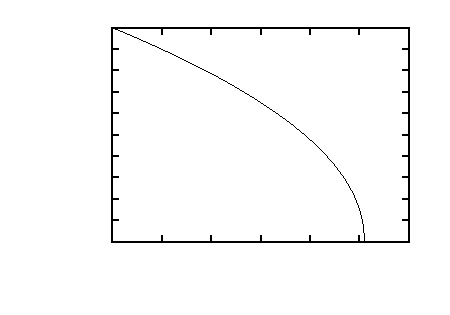
\includegraphics{chNucDissolveTimeLumPFP}}%
    \gplfronttext
  \end{picture}%
\endgroup
}
  \subfloat[Dissolution time as a function of radius]{\label{fig:nuc:dissolve_timePFP}% GNUPLOT: LaTeX picture with Postscript
\begingroup
  \makeatletter
  \providecommand\color[2][]{%
    \GenericError{(gnuplot) \space\space\space\@spaces}{%
      Package color not loaded in conjunction with
      terminal option `colourtext'%
    }{See the gnuplot documentation for explanation.%
    }{Either use 'blacktext' in gnuplot or load the package
      color.sty in LaTeX.}%
    \renewcommand\color[2][]{}%
  }%
  \providecommand\includegraphics[2][]{%
    \GenericError{(gnuplot) \space\space\space\@spaces}{%
      Package graphicx or graphics not loaded%
    }{See the gnuplot documentation for explanation.%
    }{The gnuplot epslatex terminal needs graphicx.sty or graphics.sty.}%
    \renewcommand\includegraphics[2][]{}%
  }%
  \providecommand\rotatebox[2]{#2}%
  \@ifundefined{ifGPcolor}{%
    \newif\ifGPcolor
    \GPcolorfalse
  }{}%
  \@ifundefined{ifGPblacktext}{%
    \newif\ifGPblacktext
    \GPblacktexttrue
  }{}%
  % define a \g@addto@macro without @ in the name:
  \let\gplgaddtomacro\g@addto@macro
  % define empty templates for all commands taking text:
  \gdef\gplbacktext{}%
  \gdef\gplfronttext{}%
  \makeatother
  \ifGPblacktext
    % no textcolor at all
    \def\colorrgb#1{}%
    \def\colorgray#1{}%
  \else
    % gray or color?
    \ifGPcolor
      \def\colorrgb#1{\color[rgb]{#1}}%
      \def\colorgray#1{\color[gray]{#1}}%
      \expandafter\def\csname LTw\endcsname{\color{white}}%
      \expandafter\def\csname LTb\endcsname{\color{black}}%
      \expandafter\def\csname LTa\endcsname{\color{black}}%
      \expandafter\def\csname LT0\endcsname{\color[rgb]{1,0,0}}%
      \expandafter\def\csname LT1\endcsname{\color[rgb]{0,1,0}}%
      \expandafter\def\csname LT2\endcsname{\color[rgb]{0,0,1}}%
      \expandafter\def\csname LT3\endcsname{\color[rgb]{1,0,1}}%
      \expandafter\def\csname LT4\endcsname{\color[rgb]{0,1,1}}%
      \expandafter\def\csname LT5\endcsname{\color[rgb]{1,1,0}}%
      \expandafter\def\csname LT6\endcsname{\color[rgb]{0,0,0}}%
      \expandafter\def\csname LT7\endcsname{\color[rgb]{1,0.3,0}}%
      \expandafter\def\csname LT8\endcsname{\color[rgb]{0.5,0.5,0.5}}%
    \else
      % gray
      \def\colorrgb#1{\color{black}}%
      \def\colorgray#1{\color[gray]{#1}}%
      \expandafter\def\csname LTw\endcsname{\color{white}}%
      \expandafter\def\csname LTb\endcsname{\color{black}}%
      \expandafter\def\csname LTa\endcsname{\color{black}}%
      \expandafter\def\csname LT0\endcsname{\color{black}}%
      \expandafter\def\csname LT1\endcsname{\color{black}}%
      \expandafter\def\csname LT2\endcsname{\color{black}}%
      \expandafter\def\csname LT3\endcsname{\color{black}}%
      \expandafter\def\csname LT4\endcsname{\color{black}}%
      \expandafter\def\csname LT5\endcsname{\color{black}}%
      \expandafter\def\csname LT6\endcsname{\color{black}}%
      \expandafter\def\csname LT7\endcsname{\color{black}}%
      \expandafter\def\csname LT8\endcsname{\color{black}}%
    \fi
  \fi
  \setlength{\unitlength}{0.0500bp}%
  \begin{picture}(4320.00,3024.00)%
    \gplgaddtomacro\gplbacktext{%
      \csname LTb\endcsname%
      \put(946,704){\makebox(0,0)[r]{\strut{}$10^{-1}$}}%
      \put(946,1047){\makebox(0,0)[r]{\strut{}$10^{0}$}}%
      \put(946,1389){\makebox(0,0)[r]{\strut{}$10^{1}$}}%
      \put(946,1732){\makebox(0,0)[r]{\strut{}$10^{2}$}}%
      \put(946,2074){\makebox(0,0)[r]{\strut{}$10^{3}$}}%
      \put(946,2417){\makebox(0,0)[r]{\strut{}$10^{4}$}}%
      \put(946,2759){\makebox(0,0)[r]{\strut{}$10^{5}$}}%
      \put(1078,484){\makebox(0,0){\strut{}$10^{-2}$}}%
      \put(2026,484){\makebox(0,0){\strut{}$10^{-1}$}}%
      \put(2975,484){\makebox(0,0){\strut{}$10^{0}$}}%
      \put(3923,484){\makebox(0,0){\strut{}$10^{1}$}}%
      \put(176,1731){\rotatebox{-270}{\makebox(0,0){\strut{}dissolution time (s)}}}%
      \put(2500,154){\makebox(0,0){\strut{}initial radius ($\mu$m)}}%
    }%
    \gplgaddtomacro\gplfronttext{%
      \csname LTb\endcsname%
      \put(2662,2586){\makebox(0,0)[r]{\strut{}saturated}}%
      \csname LTb\endcsname%
      \put(2662,2366){\makebox(0,0)[r]{\strut{}unsaturated}}%
    }%
    \gplbacktext
    \put(0,0){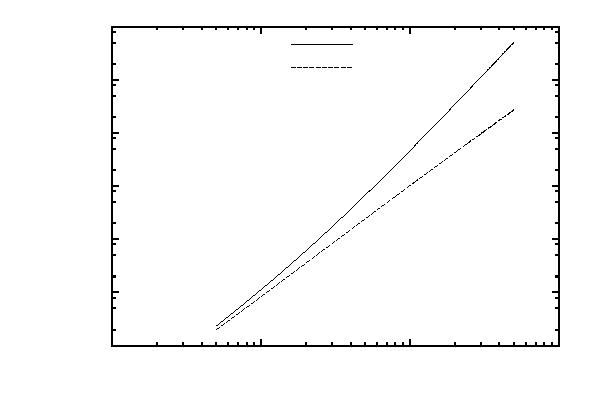
\includegraphics{chNucDissolveTimePFP}}%
    \gplfronttext
  \end{picture}%
\endgroup
}
  \caption{ Dissolve times of \pfp\ bubbles.  The experimental quantities used in the model are given in \tabref{nuc:dissolveVars}. }
 \label{fig:nuc:dissolve_time_lum}
\end{figure}


\ctable[cap=Dissolution symbols,
        caption=Symbols used in the calculation of dissolution times,
        label=table:nuc:dissolveVars,
        pos=top,
        %width = 0.6\textwidth,,,
        left
       ]
       {llllrrc}
{\tnote{Estimated with the Hayduk-Laudie equation}
}{\FL
  &   Symbol     & Description & units &Value (Air) & Value (PFP) & 
  \ML
    &$\gamma$ &   Surface tension &$\newton/\metre$ &  ${0.07280}$ \cite{Sarkar2009}   & ${0.0096828}$ \cite{NISTdata}    &
    \ML
   % &H  & Henry's constant & ${\{1.48472\times 10^{-7}} \metre^2 \kilo\gram \second^{-2} \mole^{-1}$\cite{Sarkar2009}  &  $ {3.54634\times 10^{-4}} \metre^2 \kilo\gram \second^{-2} \mole^{-1}$\cite{CASPFP}   &  
    &$H$ & Henry's constant   &$\metre^2 \kilo\gram \second^{-2} \mole^{-1}$ &  ${1.48472\times 10^{-7}} $\cite{Sarkar2009}   &  $ {3.54634\times 10^{-4}}$\cite{CASPFP}     &
    \ML
    &$D$ & Diffusivity   &$\metre^2 \second^{-1} $ &  ${2.05\times 10^{-9}} $\cite{Sarkar2009}   &  $ {6.409\times 10^{-10}}$\tmark     &
 %   &H  & Henry's constant &   &   &  
   \ML
   &$P_\infty$&  Ambient Pressure & $\mega\pascal$ & ${0.101325}$ &${0.101325}$ &
    \LL
  }

The third and final question of this chapter regards the expected lifetime of a bubble.
In \secref{nuc:evacuate} the critical radius was used to give a lower bound on the size of a 
bubble generated in a perfluorocarbon droplet or evacuated from a moat.
It was seen that bubbles in the tens of nanometres can be stable when placed under 
tension by the rarefactional cycles of an acoustic field.
The expected lifetime of the bubble after the rarefaction has passed will now be calculated.

This section uses a very simple model that was first derived by Epstein and Plesset\cite{Epstein1950},
although we prefer the notation of Gor\cite{Gor2011}.
The hope is to obtain only an order of magnitude estimate of the bubble lifetime
and so some accuracy can be foregone.

In the model a gas bubble is placed in a fluid of uniform pressure,
where the medium in the vacinity of the bubble contains the gas at concentration $n_o$.
Two gas bubbles will be considered, 
an air bubble that contains nitrogen and oxygen,
and a perfluoropentane bubble.
In each case it will be assumed that the bubble contains no water vapour,
and that the surface of the bubble is has no stabailising shell\footnote{%
See Sarkar\cite{Sarkar2009} for a recent discussion of the dissolation of a bubble that has  a permeable shell.%
}.
The concentration of the medium far from the bubble is denoted $n_\infty$
and is chosen to be the ambient density of the gas in the medium at standard temperature, $T$, and pressure, $p_\infty$.
While we imagine the bubble to be generated in a rarefaction cycle of an acoustic wave
we neither model the generation of the bubble nor the sound pulse.


There are two cases of particular interest
\nlist{
\item
  when the concentration of dissolved gas in the bubble's vacinity  is equal to the ambient concentration,
   \begin{align}
    n_0 &= n_\infty.
  \end{align}
  Such will be the case when a bubble in generated in a medium that is unaltered by the passing of the acoustic wave.
  This will typically be the case for short pulses of low pressure.
\item 
  when the concentration of the gas in the bubble's vacinity is much lower than the ambient concentration. 
  This situation can arise when a previous pulse of a high pressure wave has already evacuated most of the gas in the focal zone.
  The limiting case is when 
   \begin{align}
    n_0 &= 0.
  \end{align}
}
It is therefore natural to frame the derivation in terms a dimensionless measure of saturation,
\begin{align}
  \zeta &\equiv \frac{n_0 - n_\infty}{n_\infty }\label{eqn:nuc:saturation}
\end{align}
The two cases of interest are  when $\zeta = 0$ and $\zeta = -1$.
The solubility of the medium will make a second useful dimensionless quantity\cite{Gor2011}
\begin{align}
  s &\equiv \frac{\kB T n_\infty}{P_\infty} \label{eqn:nuc:solubility}.
\end{align}

Imbalances in the number density of the gas in the medium will prompt diffusion from the vacinity of the bubble to the bulk.
Modelling this as Fickian diffusion  in a spherical geometry gives,
\begin{align}
  j_D = -D \frac{\partial n}{\partial r}
  \label{eqn:nuc:Fickian}
\end{align}
where  the density is a spherical symmetric function of radius, $r$.
If diffusion transport terms are neglected then \eqnref{nuc:Fickian} can be solved to obtain,
\begin{align}
  \frac{\partial n}{\partial r} = \lr{n_R - n_0}\lrsquare{\frac{1}{R} + \frac{1}{\sqrt{\pi D t}}},
\end{align}
where $R$ is the bubble radius and $n_R$ is the concentration of dissolved gas at that radius.
The details of the derivation were given in Epstein and Plesset's \cite{Epstein1950} original paper and do not need to be reproduced here.

Material conservation requires that the number of particles passing through the radius of the bubble
equates to the change in the number of particles in the bubble, $N$,
\begin{align}
  \frac{dN}{dt} =4 \pi R^2 j_D\frac{\partial n}{\partial r}.
\label{eqn:nuc:materialCons}
\end{align}

Modelling the contents of the bubble as an ideal gas lets the particle number be expressed in terms of the ambient pressure, $P_\infty$, and surface tension $\gamma$ of the bubble,
\begin{align}
  N = \frac{4\pi R^3 }{3\kB T} \lrsquare{P_\infty + \frac{2\gamma}{R}}.
  \label{eqn:nuc:ParticleNumber}
\end{align}
By differentiating \eqnref{nuc:ParticleNumber} and equating the result to \eqnref{nuc:materialCons} a differential equation for the change in bubble radius is obtained,
\begin{align}
   \dot{R}\lrsquare{ 1+ \frac{4\gamma}{P_\infty R}} = Ds\lrsquare{ \zeta - \frac{2\gamma}{P_\infty R}}\lrsquare{\frac{1}{R} + \frac{1}{\sqrt{\pi D t}}},
   \label{eqn:nuc:Rdot}
\end{align}
where equation \eqnref{nuc:solubility} has been used, along with
\begin{align}
  \frac{\lr{n_0 - n_R}}{n_\infty} = \zeta - \frac{2\gamma}{P_\infty R}
  \label{eqn:nuc:dissolve}
\end{align}
which follows from \eqnref{nuc:saturation}.






The numerical solution of \eqnref{nuc:dissolve} is plotted for a 1 micron air bubble in \figref{nuc:dissolve_time_lum}.
It is seen that the bubble radius decreases fairly constantly until a very rapid final callapse.
The lack of a long tail in \figref{nuc:dissolve_time_lum}
means that the dissolution time is dominated by periods when the bubble is near is starting radius.
There is not a long decay during which the bubble is technically existent but is so small as to be unobservable.

The dissolution time for an air bubble as a function of radius is plotted in \figref{nuc:dissolve_time}.
Both the saturated and unsaturated cases are plotted.
The dissolution times for very small bubbles is very similar,
but starts to diverge for bubbles of radius \unit{0.5}\micro\metre.

The lifetime of a free submicron air bubble is of order \unit{1}\milli\second\ in both the  saturated and unsaturated cases.
The pulse duration of diagnostic ultrasound is typically measured in microseconds and so the bubble would be expected to live throughout the duration of the pulse.
However, adjacent alines in a diangostic pulse are often tens of milliseconds apart.
Submicron air bubbles would not be expected to exist in adjacent alines.
The short lifetimes of air bubbles mean that care needs to be taken to syncronise the generation and the imaging of a bubble,
so that the imaging wave samples the same focal region as the driving wave within a few microseconds of the driving wave passing.
%In this case the observable rate of nucleation given is given by equation \eqnref{nuc:rateOne}.


The solubility of the perfluorocarbons in water is much lower than for nitrogen and oxygen.
While the dissolution characteristics are very similar to an air bubble (\figref{nuc:dissolve_timePFP})
the timescale for dissolution is order of magnitudes larger (\figref{nuc:dissolve_time_lumPFP}).
This has the advantage that a bubble can be generated at a different time (and therefore at a different location)
to where the bubble is imaged.
In this case  the driving wave and the imaging wave can be considered independently.

\section{Discussion}\label{sec:nuc:discussion}

\subsection{Summary of results}

In this chapter the two broad approaches of generating a bubble with sound for the purpose of imaging are analysed.

On the one hand one may attempt to create a bubble via type I nucleation.
The pressures required to do so in water are beyond the capabilities of diagnostic ultrasound
and so one may instead focus on creating an emulsion with a second medium that is easier to nucleate.
The perfluorocarbons, due to their low boiling points, low solubility and low toxicity make excellent 
candidates.
This chapter has suggested by means of the capillary approximation that very few perfluoro-molecules are 
needed to create a bubble, and that the nucleating pressure is much reduced - down to \unit{7-8}\mega\pascal\ negative pressure for
perfluoropentane
These pressures are still on the cusp of what is used in medical ultrasound
and are still beyond what can be achieved with a diagnostic transducer.
However, given the questions regarding the approximation's accuracy that are raised by the calculated number of nucleating molecules 
- in the tens and low hundreds - 
the perfluorocarbons still most definitely represent a contrast medium that is worthy of experimental study.

On the other hand one may abandon type I and type II nucleation altogether and focus on extracting gas that is stabilised in impure water.
The main difficulties in this approach is to control the impurities in the water so that small bubbles are not overwhelmed by larger bubbles,
and to image the generated bubble within its millisecond lifetime.
Generating bubbles at diagnostic pressures is not a challenge in this approach.
Indeed, great pains are usually gone through in ultrasound experiments to prevent such bubble generation.

A certain degree of control can be exerted on the size of bubble generated in by type III nucleation.
From \eqnref{nuc:Rdot} the critical radius of an air bubble is found to be
\begin{align}
  R^\ast = \frac{2 \gamma}{\zeta P_\infty}.
\label{eqn:nuc:astarTwo}
\end{align}
The Laplace relation, \eqnref{LaplaceRelation}, cannot be used as it  focuses solely on vapour bubbles.
The saturation, $\zeta$, can be plotted as a function of pressure by using Henry's law,
which finds that density a gas in water is proportional to the applied pressure,
\begin{align}
  P = H n,
\end{align}
where $H$ is Henry's constant.  One finds that 
\begin{align}
  R^\ast = \frac{2\gamma}{n_0H - P_\infty}.
\end{align}
Since the critical radius provides a lower bound on the size of the evacuated bubble,
equation \eqnref{nuc:astarTwo} provides an estimated on the size of bubble that is generated in dirty water.
%Equation \eqnref{nuc:astarTwo} is plotted in \figref{nuc:astarTwo}.




%\subsection{Structure of the chapter}

%The two mechanisms are analysed by asking the following questions,
%The first step is then 
%\nlist{
%  \item as a function of the driving waves peak-negative pressure, what size bubble is expected to be evacuated from a mote?
%  \item at what pressures are submicron perfluorocarbon droplets expected to vaporise?
%}


%\Secref{nuc:radius} then completes the calculations of \secref{nuc:evacuate} and \secref{nuc:vapourise}
%by evaluating the critical radius.
%This is achieved with two semi-empirical approaches
%that fit theoretical parameters such as the critical radius
%to the following thermodynamic properties of the water/oil droplet:
%%To calculate the rate of nucleation the following experimental data must be provided\cite{Nyquist1995}:
%\nlist{
%  \item the density of the liquid,
%  \item the equilibrium vapour pressure,
%  \item the equilibrium surface tension between liquid and vapour.
%
%}

%The first model, introduced in \secref{nuc:cnt}, uses the capillary approximation to find the critical radius.
%In this approximation both liquid and vapour are assumed to be at their respective bulk densities with a sharp interface between the two.
%The surface tension is taken to be that of the macroscopic plainer interface.


%In \figref{cnt:critical_radius}  the critical radius as a function of pressure is plotted  for water, perfluoropentane and perfluorobutane.
%\Cnt\ predicts that the critical radius is smaller for the perfluorocarbons than for water.
%This is  encouraging, for it implies that type 1 nucleation is easier to induce for the perfluorocarbons than for water.
%%However, the critical radii predicted are  somewhat large for our application.
%A \unit{20}\nano\metre-radius bubble represents more than 10\% of the radius of the oil-droplet.
%This undermines the assumption made that  neglects boundary between the oil droplet and the water.
%On the other hand, the capillary approximation is likely to be less severe.

%At high pressures the critical radii of the two perfluorocarbons converge.
%This is because the critical radius depends linearly on the surface tension (equation \eqnref{LaplaceRelation})
%and the surface tension are similar for perfluorocarbons.
%At lower pressures the vapour pressure has a much greater role, which is higher in the case of perfluorobutane.
%It should be noted that the vapour pressure used for perfluorobutane was extrapolated by \unit{29}\degreecelsius\  outside of its range of validity\cite{NISTdata}
% by use of Antoine's equation.
%Since \unit{25}\degreecelsius\ is above the boiling point of perfluorobutane no  equilibrium vapour pressure can be defined.
%However, since \unit{25}\degreecelsius\ is also well below the critical temperature, % (\tabref{:nuc:criticalTemps}), 
%and so it is hoped that the predicted pressures within the (super-heated) bubble are still meaningful.
%The other parameters are taken from \tabref{nuc:parameters}.


%In \figref{cnt:critical_number}  the predicted number of molecules contained within a critical bubble are plotted.
%Again, the number of perfluorocarbon molecules required to form a bubble are smaller than if the for water.
%\Figref{cnt:critical_number} does, however, illustrate  the difficulty with the capillary approximation being used.
%It is highly questionable that a bubble containing so few molecules behaves like its thermodynamic bulk,
%with a constant density until the interface.
%\Cnt\ predicts that a greater number of molecules are required to form a critical bubble for perfluorobutane than for perfluoropentane.
%This is again due to the higher vapour pressure of  perfluorobutane.

%(A 20\nano\metre-diameter bubble {\em is} large to materialise by spontaneous fluctuation)
%the resulting bubble is not predicted to  contain too many molecules.
%The number of molecules within a critical bubble is perhaps more suggestive.
%This is the number of molecules that must join a bubble by fluctuation before it can grow.
%Again the number is far fewer for perfluoropentane than water.

%It is worthwhile estimating the number of molecules within the perfluoropentane bubble.
%For example, at a  negative pressure of \unit{1}\mega\pascal\ the critical radius
%of perfluoropentane is predicted to be \unit{8.7}\nano\metre\ at a vapour pressure of \unit{0.927}\ atmospheres.
%Assuming that the vapour behaves as an ideal gas, we find that the bubble contain approximately 60 molecules.


%\Figref{nucleation_radius} plots the critical radius of a bubble as a function of the liquid pressure.
%At low pressures, the capillary approximation is not significant.
%The density profile of \figref{profile} shows that the interface extends over only a nanometre or so.
%However, \figref{cnt:rate} shows that the nucleation rate is incredibly slow at these pressure.
%By comparing the graphs it is seen that it is exactly when the rate becomes appreciable, 
%when \figref{profile} shows the rate to become invalid.

\subsection{Concerns with the capillary approximation}\label{sec:nuc:CAvalid}

The assumptions of the capillary approximation are problematic when the nucleating bubble is very small\cite{Talanquer1995}
because the distance over which the density changes from liquid to vapour is not insignificant
and because the surface tension is typically reduced from its bulk value\cite{Kiang1971}.
%For instance, %deviations in the surface tension from the bulk value take exponential importance in the rate calculations
%necessary to determine the pressure required to observe a nucleation event.
%an increase in the surface tension of 15\%
%was calculated\cite{Kiang1971} to change the predicted nucleation rate by $10^{17}$.
%Another example is provided by the calculations of Talanquer and Oxtoby\cite{Talanquer1995, Oxtoby1988}.
%Their  density functional calculations 
%predicted that the rates  from these  calculations were  {\em typically}   20 orders of magnitude different from those of \cnt.

%To overcome these difficulties we employ the semi-empirical density functional approach of Nyquist\cite{Nyquist1995} and Talanquer\cite{Talanquer2001} in \secref{nuc:DFT}.
%An improvement on the capillary approximation is achieved by  relaxing
%the requirement for sharp interfaces between liquid and vapour.
%Instead, a model for the intermolecular forces is used to evaluate the transition from liquid to vapour.
%The model parameters are then fitted to the fluids bulk thermodynamic properties.
%%
%

Deviations from the capillary approximation are exponentially important in rate calculations,
which follows from the Arrhenius equation.
%This is because the thermodynamic part of the calcuations
For example, an increase in the surface tension of 15\%
was calculated\cite{Kiang1971} to change the predicted nucleation rate by $10^{17}$.
Another example is provided by the calculations of Talanquer and Oxtoby\cite{Talanquer1995, Oxtoby1988}.
Their  density functional calculations, that relaxes the requirement for sharp interfaces between liquid and vapour,
predicted that the rates  from these  calculations were  {\em typically}   20 orders of magnitude different from those of \cnt.
% to  allow the density profile to change more  realistically from the step jump assumed in the classical theory.
%The rates  from these  calculations were  {\em typically}   20 orders of magnitude different from those of \cnt.
%In order to bound our calculations, we use the density functional approach to evaluate the spinodal.
%This is the point at which the energy barrier vanishes and a phase decomposition is guaranteed to occur\cite{Favvas2008}.


 % \todo{comment on previous work}
 % Before we start however, 
 % we note that perfluorocarbon droplets have successfully been vapourised with ultrasound before,
 % and indeed has a fairly long history.
 % Kripkins was amongst the first to demonstrate the technique in an attempt to form a large bubble to obficate blood vessels.
 % More recently ... in Toronto has found that bubbles of perfluorpentane (with a boiling point of 28 degrees) can be vaporised with long bursts of ultrasound.
 % Additionally they found that the surfactant was very important.  With some surfactants they were able to increase the rate of nucleation,
 % with others they were not.  Their initial success was with Zonyl ..., a somewhat toxic and explosive substance, although seeminly tolerated by mice in the small quantities used.
 % A type 1 nucleation agent should not be impossible for diagnostic ultrasound.

% Finally, in this chapter we would like to emphasise a reoccuring theme in this thesis.
% And that is that the variables that we may measure experimentally are not, in general independent of the process of measurement.
% This is particularly the case in statistical physics.
% As the quote that introduces this chapter emphasises, 
% the entropy, of central importance in the following discussion,
% is not a propterty of the physical system at all - but is entirely a function of what experiment is carried out.



% \section{Nucleation of a small oil droplet}

% As argued, the nucleation of a small droplet is likely to occur in the absence of motes and pre-existing stabalised vapour bubbles.

% The simplest approach to estimating the nucleation rate of the oil droplet is to 
% assume that the droplet is the `bulk fluid' and estimate the rate of type 1 nucleation events within it.
% We do this first within the framework of \cnt\ in \secref{nuc:CNT}.

% Superheating often brings near critical region where mean field approach fails so concentrate on negative pressure \cite{Oxtoby1988}.

% Cavitation does not parallel condenstaion\cite{Oxtoby1988}.
% the spinodal is much close tot h phase coexstance curve n the iquid side thana on the gas, 
% therefore the spinodal exerts a large influence on ucleation and  clasical theoory fails\cite{Oxtoby1988}.



%This ignores the finite size of the droplet.
%However


% For some applications \cnt\ works well, particularly in determining the supersaturation limit of the oil.
% However,  the bubble nucleation rate predicted by the classical theory 
% is generally poor\cite{Talanquer1994} with discrepancies of 20 orders of magnitude with more accurate calculations typical\cite{Talanquer1994}).
% The reason is that the macroscopic thermodynamics enters  the exponential of the Aarenhius  equation,
% upon which the rate is incredibly sensitive.
% To predict the pressures at which the perfluocarbons nucleate,
% we need to handle the thermodynamics of bubble nucleation with greater care.



%As mentioned, classical nucleation theory represents a semi-empirical theory
%which is obtained with
%\nlist{
%  \item the density of the liquid,
%  \item the equilibrium vapour pressure,
%  \item the equilibrium surface tension between liquid and vapour.
%}

%The free energy of a gas, $\Omega_G$ in this region will therefore be lower than the bulk liquid $\Omega_L$.
%On the other hand, the creation of the bubble has the cost of creating the surface tension.
%The change in the grand potential will therefore be
%\begin{align}
%\Delta \Omega(a) = \frac{4}{3}\pi a^3 \lr{\Omega_G - \Omega_L} + 4 \pi a^2. \label{eqn:nuc:DeltaOmega}
%\end{align}
%The first term is negative, but the second positive.
%Small bubbles are dominated by the surface tension and are accordingly unfavorable.
%There is therefore, a {\em critical radius} $\astar$ at which the energy gap vanishes and the 
%bubble will form.%

%The problems of the capillary approximation in relation to bubble nucleation
%have already been discussed.
%We have also pointed out where the approximations become problematic in the calculations provided.
%While \cnt\ provides a useful point of departure for rate estimates,
%the theory is too simplistic to be definitive.

The version of the \cnt\ used here is perhaps the simplest that can be used.
There are many modifications that alter in some way the exponential in \eqnref{nuc:J},
and thereby drastically altering the rate predictions.
The problems of the capillary approximation are common to all classical theories, however, 
and so the simple application here is representative.

Perhaps the most relevant of the modified classical theories is the careful application to bubble nucleation carried out by Delale\cite{Delale2003}.
In addition to the problems associated with the capillary approximation,
Delale notes that it is unlikely in ultrasound applications for cavitation to proceed on a reversible path, as is assumed.
Furthermore, the viscous dampening at the bubble-oil interface, which is known to be important in bubble dynamics, mean that 
at thermodynamic equilibrium (when the bubble's radius is at its critical size),
the bubble is not in mechanical equilibrium.
Delale\cite{Delale2003}  convincingly argues for a phenomenological term should be added to the Gibbs energy difference to correct for these problems.
Unfortunately the terms of this correction are difficult to ascertain far from the critical temperature.
It is therefore difficult to apply Delale's theory in this thesis\cite{Delale2003}.




%In \figref{cnt:rate} it is seen that \cnt\
%predicts that the nucleation of \pfp\ becomes observable at \unit{-7}\mega\pascal,
%\pfb\ nucleation becomes observable at \unit{-8}\mega\pascal\ 
%and water nucleation becomes observable at \unit{$\approx$-105}\mega\pascal.
%These results are somewhat  discouraging, % they are much higher than what can be achieved with a diagnostic probe.
%for while the nucleation rate is much greater than that of water,
%such pressures are still tremendously high for diagnostic ultrasound.
%However,
%as has already been discussed,
%it is common for \cnt\ to severely underestimate the nucleation rate.
%Experimentally water undergoes types 1 nucleation 
%at approximately 25\mega\pascal,
%a much lower pressure than predicted from the classical theory.
%Similar reductions for the perfluorocarbons would bring the nucleation 
%rates into experimental reach.

%\Figref{cnt:rate} is also interesting because it highlights the sensitivity
%to the exponential terms in \eqnref{nuc:J},
%and the insensitivity to the pre-exponential factor.
%It is evident that the 
%pressure required for nucleation is barely altered even if the rate 
%is altered by several orders of magnitude.
%For this reason, the theory should be insensitive to inaccuracies in the (problematic) derivation of $J_0$.

%On the other hand, the appreciable difference in the pressure pressures required to nucleate 
%perfluoropentane
%and \pfb\ result from the  10\% difference in surface tension.
%This corresponds to a 16 order of  difference between the two rates.

%There does not seem to be a wealth of surface tension measurements for perfluorobutane.
%It is not clear as to whether the surface tension of \pfb\ is genuinely higher than \pfp,
%or whether the difference between the two is from the slight difference in temperature at which the measurements are made, 
%or due to experimental uncertainty.
%Whatever the cause, 
%it is the higher value of surface tension used for \pfb\ that causes the somewhat surprising prediction that 
%\pfp\ has a higher nucleation rate than \pfb.


% Rather than give a spurious argument we prefer  here to estimate $J_0$ by dimensional analysis.
% The result is the same as that used in the literature and is obtained at a fraction of the effort.
% In addition, the estimate obtained here does not give the impression of greater accuracy than it deserves.
% A danger ever present in kinematic derivations.

% The variables that are deemed relevant are listed in \tabref{nuc:dimensional_vars} along with their dimensions.
% Listed are 5 variables comprised of 3 dimensions: mass, length and time.
% It is therefore possible to write down 2 dimensionless groups\cite{SanjoyBook}.

% % The 5 variables split into variables that characterise the bubble
% % \nlist{
% %   \item the rate of bubble growth $J_0$
% %   \item the vapour mass density, $m \rho_v$,
% %   \item the surface tension, $\gamma$,
% % }
% % and a  variable that characterise the fluid
% % \nlist{
% %   \item the liquid mass density, $\rho_L$.
% % }

% % To eliminate the temporal dependence the rate per volume, $J_0$, must be squared 
% % and combined with surface tension.
% % This resulting $J^2/\gamma$ has the units $\lrsquare{M}^{-1}\lrsquare{L}^{-6}$,
% % where the square brackets denote the units of mass and length, respectively.
% % These quantities can be cancelled from the mass of the fluid, $m$, 
% % and the square of a number density.
% % There is a choice as to which number density should be used.
% % The density of the liquid $\rho_L$, or the number density of the vapour, $\rho_v$.

% The first is 
% \begin{align}
%   \Pi_1 &= \frac{J_0^2 m}{\gamma\rho_v^2}.
%  \intertext{The vapour number density, $\rho_v$, chosen here rather than the liquid number density $\rho_L$. 
%    $\rho_v$ is more appropriate since  $J_0$ is the high temperature limit.
%  The second dimensionless group is the ratio of the densities,}
%   \Pi_2 &= \frac{\rho_L}{\rho_v}.
% \end{align}
% Writing $\Pi_1$ as some function, $g$, of $\Pi_2$ we obtain,
% \begin{align}
%   J_0 = \rho_v \sqrt{\frac{\gamma}{m}} g\lr{\frac{\rho_L}{\rho_v}}.
% \end{align}
% The function $g$ is undetermined, however, it may be argued on physical grounds.

% If the number density of the liquid is increased above equilibrium, then the excess chemical potential will be balanced if  molecules 
% leave the fluid and enter the bubble.
% The nucleation rate should therefore increase with $\rho_L$.
% Conversely,  the nucleation rate should  decrease with an increased vapour density, $\rho_v$.
% The simplest such relationship between rate and density is a linear one, 
% and so we guess $g(x) \propto x$.
% If the constant of proportionality is assumed to be approximately unity, then 
% for  bubble nucleation we have
% \begin{align}
%   J_0 \approx \rho_L \sqrt{\frac{\gamma}{m}} g\lr{\frac{\rho_L}{\rho_v}}.
% \end{align}
% This is the conventional form for the pre-exponential factor in bubble nucleation.

% Sometimes 

% the rate should decrease with density of the vapour density, $\rho_v$.

% If $g = 1$ then 
% If however, 
% Writing $g(x)= x$ gives


% The most general function of the variables $\Pi_1$ and $\Pi_2$ is
% \begin{align}
%   f(\Pi_1, \Pi_2) = 0. \label{eqn:nuc:roots}
% \end{align}
% If $Pi_2$ is held fixed then \eqnref{nuc:roots} may be written fixed we examine the family of roots 
% \begin{align}
%   f_{\Pi_2}(\Pi_1) = 0,
% \end{align}
% of which the solution is $Pi_1 = f(

% The second of these 


% The resulting constant is the same as that which is used in the literature, 
% without 
% but 


% It is not entirely clear, however, what is meant by a `cluster bubble'. 
% Conceiving a bubble as a cluster of  gas molecules is difficult conceptually, however.






% Rather, the rate can be estimated from a kinematic argument 
% by estimating the rate at which individual molecules impinge upon and then leave the bubble\cite{Katz1992}.
% The number density of bubbles containing $i$ molecules is needed for the calculation
% and we obtain this from the thermodynamic argument by assuming that 
% the number density is distributed according to a Boltzmann distribution%
% \footnote{A Boltzmann distribution is the least prejudicial view\cite{Jaynes1957a}},
% \begin{align}
%   C_i =n \exp \lr{- \frac{\Delta G}{\kB T}}, %= N \exp\lr{- \frac{16\pi\sigma^3}{3\kB\lr{p_v^\ast - p_L} T}},
%   \label{eqn:CnBoltzman}
% \end{align}
% where $n$ is the  number density of molecules in the fluid.

% The resulting rate equation  is 
% \begin{align}
%   J = J_0 \exp\lr{- \frac{16\pi\sigma^3}{3\kB T\lr{p_v^\ast - p_L}^2}}, \label{eqn:nuc:J}
% \end{align}
% where 
% \begin{align}
%   J_0 = S^{i^\ast}
%   \frac{p_v n}{  \rho_v^\ast\kB T}\sqrt{\frac{2\sigma M_r}{\pi }}
%   \label{eqn:nuc:Jzero}
% \end{align}
% and  $i^\ast = \frac{4\pi \astar^3 \rho_v^\ast}{3 M_r}$ is the critical number of molecules in the bubble and $M_r$ is the molecular weight.
% The derivation $J_0$ is reproduced in \appref{CNT}.
% It is originally from Katz\cite{Katz1992},
% although we prefer the notation of McClurg\cite{McClurg},
% and so it is this that is given.


% we need to know the number density of bubbles containing $i$ molecules.
% We denote this density $C_i$ and assume that is  distributed according to a Boltzmann distribution%
% \footnote{A Boltzmann distribution is the least prejudicial view\cite{Jaynes1957a}},
% \begin{align}
%   C_i =n \exp \lr{- \frac{\Delta G}{\kB T}}, %= N \exp\lr{- \frac{16\pi\sigma^3}{3\kB\lr{p_v^\ast - p_L} T}},
%   \label{eqn:CnBoltzman}
% \end{align}
% where $n$ is the  number density of molecules in the fluid.



% To find the rate of nucleation we cannot use equilibrium thermodynamics.
% We give McClurg's\cite{McClurg} version of the derivation of Katz\cite{Katz1992} in \appref{CNT}.
% The result is that
% \begin{align}
%   J = J_0 \exp\lr{- \frac{16\pi\sigma^3}{3\kB T\lr{p_v^\ast - p_L}^2}}, \label{eqn:nuc:J}
% \end{align}
% where 
% \begin{align}
%   J_0 = S^{i^\ast}
%   \frac{p_v n}{  \rho_v^\ast\kB T}\sqrt{\frac{2\sigma M_r}{\pi }}
%   \label{eqn:nuc:Jzero}
% \end{align}
% where $i^\ast = \frac{4\pi \astar^3 \rho_v^\ast}{3 M_r}$ is the critical number of molecules in the bubble and $M_r$ is the molecular weight.







% At $a = \astar$ the probability of the bubble expanding is equal to the probability of the bubble contracting,
% and so (an unstable) thermodynamic equilibrium has been reached.
% This implies that the chemical potentials are equal
% \begin{align}
%   \mu_v(p_v^\ast) = \mu_L(p_L),\label{eqn:thermoEqlbm} \quad\text{ at $a = \astar$.}
% \end{align}

% The critical radius alternatively be expressed 
% \begin{align}
%   \astar = \frac{2\sigma}{\rho_L \kB T \ln S}
% \end{align}
% where $S \equiv \frac{p_v}{p_\infty}$ is the supersaturation ratio.
% To obtain this expression we assume that the oil is incompressible so that 
% \begin{align}
%   p_v - p_L = 
% \end{align}

%The vapour pressure is evaluated from the Antoine equation, with the coefficients taken from Barber\cite{Barber1956}.



% To find the rate of nucleation we cannot use equilibrium thermodynamics.
% We give McClurg's\cite{McClurg} version of the derivation of Katz\cite{Katz1992} in \appref{CNT}.
% The result is that
% \begin{align}
%   J = J_0 \exp\lr{- \frac{16\pi\sigma^3}{3\kB T\lr{p_v^\ast - p_L}^2}}, \label{eqn:nuc:J}
% \end{align}
% where 
% \begin{align}
%   J_0 = S^{i^\ast}
%   \frac{p_v n}{  \rho_v^\ast\kB T}\sqrt{\frac{2\sigma M_r}{\pi }}
%   \label{eqn:nuc:Jzero}
% \end{align}
% where $i^\ast = \frac{4\pi \astar^3 \rho_v^\ast}{3 M_r}$ is the critical number of molecules in the bubble and $M_r$ is the molecular weight.

% Equation \eqnref{nuc:J} is perhaps the simplest of many variants.
% For instance, type 2 nucleation can be incorporated by included a prefactor to $\Delta G$.
% The reduction  in nucleation energy is because the surface that needs to be created is smaller when a bubble forms within a crevice,
% and the technique is review by Lubetkin\cite{Lubetkin1995}.
% Type 2 nucleation is not of primary interest, however, and so we do not pursue this technique here.




%Type I nucleation of perfluoropentane will be characterised in \secref{nuc:typeOne},
%the evacuation of a bubble from 

% The second objective is to determine the pressures at which a submicron perfluorocarbon droplet vaporises.
% %Although creating a bubble via type I nucleation is very different than evacuating entrapped gas,
% Again, the key step in this calculation is the evaluation of the critical radius. % of the bubble.
% The thermodynamic fluctuation that forms a nascent bubble 
% will dissolve away if the critical radius is not reached.
% %  t reach the critical radius to prevent the bubble from instantly dissolving away.
% It defines the energy required for the bubble to form,
% from which %The critical radius enables the energy barrier to forming a bubble to be calculated via the Arrhenius equation.
% the probability of a type I nucleation event follows.
% The calculation is introduced in \secref{nuc:vapourise}
% and is little more than an application of the Aarenhius equation.
% The energy barrier to nucleation is found from thermodynamic arguments,
% while the rate is obtained from a kinematic argument.

%For



%The critical radius is dependant upon the pressure of the medium.
%and is dependent on the pressure of the medium.
%The size of bubble evacuated from a mote can
%therefore be written in terms of the driving pressure.
%Evaluating this bound is the first objective of this chapter,
%and is explored in detail in \secref{nuc:evacuate}.

 %T bubble is at equilibrium with its surrounding.
%The bubble must reach this size in order to leave the bubble.

%The motivation for the first question is the possibility 
%of selecting a driving pressure that evacuates bubbles only in a narrow band of sizes.
%The driving wave could be then further be used to tune that size for a given imaging wave.
%The second question relies on the possibility of manufacturing oil droplets
%within a narrow size distribution, 
%so that their resulting bubbles are sufficiently similar in size 
%for a significant proportion of the bubbles to be resonant or tuned to resonance.

%A {\em density functional} approach is used to investigate these questions.
%Density functional theory enables the critical radius of the bubble
%to be estimated as a function of pressure.
%This is the radius at which it is energetically favourable for the bubble to grow.
%In answer of the first question, 
%the critical radius must be reached for entrapped gas to form a complete bubble and leave a mote.
%If the radius is not reached, then it will cost less energy for the bubble to remain on the 
%It thereby provides an estimate of the size of a free bubble that is  generated from a mote.
%In answer of the second, the critical radius enables the energy barrier to nucleation to be calculated,
%from which the nucleation probability follows.
%By setting a threshold probability at which observing a nucleation event is deemed likely,
%the vaporisation pressure can be calculated.



%Only submicron bubbles are interesting.

%
%
%\nlist
%{
%  \item Imaging a pre-existing, submicron bubble that has been evacuated from a mote within the bulk fluid
%    via type III nucleation.
%  \item Imaging a bubble that has been yielded from an oil based contrast via type I nucleation. \label{item:nuc:oil}
%}
%
%the pressures required to do so are prohibitively high for ultrasound.
%In this chapter we will concentrate on approach \ref{item:nuc:oil}.
%
%Basing a contrast agent upon the impurites in water is only defensible if the
%water does not
%
%This is because the cavitation threshold of many human tissues approaches the type I/II nucleation thresholds\todo{cite}.
%Biology seems very adept at preventing gas pockets from occuring.
%cavitation is not without bio-effect.
%


%\subsection{DFT}
%\section{Other discussion}

%In addition to the nucleation rate we provide an upper bound on the pressure required to induce a phase change.
%This is done by evaluating the spinodal : the point at which the energy barrier for the liquid-vapour transition vanishes (see Favvas\cite{Favvas2008} for an introduction).
%While the decomposition of phases past the spinodal is not  nucleation -
%the phases separate throughout the oil rather than forming a bubble -
%the spinodal nevertheless marks a fundamental and guaranteed  change in the contrast agent.
%However, Talanquer and Oxtoby used dissolved gasses such as oxygen and carbon dioxide as their examples of nucleation. 
%The high vapour pressures of these gases causes the critical radius of the bubble very small: just a few na
%with a corresponding  cause considered  the nucleation of highly volatile liquids  the nucleaton of volatile liquids 

%Such spectacular deviations are typical for bubble nucleation predictions. 
%On the other hand, for predicting the condensation of a vapour bubble 
%\cnt\ is often satisfactory.
%The density functional approach explained this discrepancy by finding that the 
%spinodal exerts a stronger influence on the liquid-vapour transition than its reverse\cite{Oxtoby1997}.
%\Cnt\ does not model the spinodal and the rates predicted for   evaporation and condensation are identical.
%The qualitative success of the classical theory for this transition was considered fortuitous,
%resulting from a cancellation of errors\cite{Oxtoby1997}.

%Talanquer and Oxtoby, however,


%\subsection{Other}


%The grand potential is in general difficult to evaluate, however.
%This is because the intrinsic free energy incorporates the interaction of every molecule with every other molecule in the system.
%This introduces integrals that are intractable.
%The approach of \dft\ to this problem is standard in statistical physics:
%the true probability density function, $p_0(\H; \cx_1,\cp_1)$, that describes 
%the positions of the particles and their momentums,
%is approximated to a simpler distribution $p(H; \cx_1, \cp_1)$ that may be solved.
%Here, $\H$, is the true Hamiltonian of the system 
%and $H$ is the approximate Hamiltonian with simpler interaction terms.
%We has also employed the  convenient shorthand
%\begin{align}
%\cx_n \equiv r_n,r_{n+1},\ldots,r_N,  \quad\text{and}\quad
%\cp_n \equiv  p_n,p_{n+1},\ldots, p_N.
%    \label{eqn:shorthand}
%\end{align}
%to describe the positions and momentums of  $N-n$ particles.



%\section{Classical nucleation theory} \label{sec:nuc:CNT}


%When the rarefactional pressure of the acoustic wave exceeds the atmospheric pressure it places the fluid under tension.
%The creation of a vapour bubble  relaxes this pressure but  also creates an interface.
%Creating a small bubble is energetically unfavourable because the surface tension dominates.
%A large bubble, on the other hand, will grow explosively when placed under tension because the volume term dominates.
%For a given pressure there exists, therefore, a {\em critical radius}, $\astar$, at which the bubble neither grows nor shrinks, 
%but is at thermodynamic equilibrium.

%If a bubble is created adiabatically then the energy required to form a bubble of radius $a$ is  \cite{Delale2003, Katz1973}
%\begin{align}
%  \Delta G =4\pi \gamma  a^2 - \frac{4\pi a^3}{3}\lr{p_v - p_L} + i\lr{\mu_v(p_v) - \mu_L(p_L)}.\label{eqn:DeltaG}
%\end{align}
%Here $\Delta G$ is the change in the Gibbs free energy, $\gamma$ is the surface tension and $a$ is the radius of the bubble.
%$p_L$ and $p_v$ are the pressures of the oil droplet and the vapour,
% $\mu_L(p_L)$ and $\mu_v(p_v)$ are the chemical potentials (per molecule) of the oil droplet and vapour
%at their given pressures,
%and $i$ is the number of molecules in the newly created vapour bubble.
%The first term on the right hand side of equation \eqnref{DeltaG} is the contribution from the surface tension.
%The second is the energy released by the change in volume,
%the third is the energy generated from  the chemical potential by the transport of molecules.
%
%The critical radius is  when the energy  barrier $\Delta G$ is maximal.
%By differentiating \eqnref{DeltaG} with respect to $a$ it is found to be
%\begin{align}
%  \astar = \frac{2\gamma}{p_v^\ast-p_L}, \label{eqn:LaplaceRelation}
%\end{align}
%which is the Laplace relation.
%Substituting \eqnref{LaplaceRelation} into \eqnref{DeltaG} gives the energy required to create a bubble of  critical radius,
%\begin{align}
%   \Delta G^\ast \equiv \given{\Delta G}{a = \astar} = \frac{16\pi\gamma^3}{3\lr{p_v^\ast- p_L}^2}.\label{eqn:DeltaGStar}
%\end{align}
%The chemical potentials have vanished from \eqnref{DeltaGStar} because  the bubble is at thermodynamic equilibrium, whence
%\begin{align}
%  \mu_v(p_v^\ast) = \mu_L(p_L),\label{eqn:thermoEqlbm} \quad\text{ at $a = \astar$.}
%\end{align} 
%The pressure, $p_v^\ast$, is the critical pressure within the bubble.
%Due to the bubble's curvature  it is not equal to the equilibrium vapour pressure of a flat interface, 
%denoted $p_\infty$. % (the $\infty$ being the radius of a `flat' bubble).
%The two vapour pressures are related by the Poynting correction, 
%\begin{align}
%  p_v^\ast = p_\infty \exp \lr{ \frac{V_m\lr{p_L -p_\infty} }{R T}  },\label{eqn:PoyntingCorrection}
%\end{align}
%where $V_m$ is the molar volume  and $R$ is the ideal gas constant.
%Equation \eqnref{PoyntingCorrection} is derived, for completeness, in  \appref{CNT}.


%Another variation on equation \eqnref{nuc:J} enables type 2 nuclation to be encorporated.
%The reduction in the surface area of a bubble provided by a crevice can be included as a prefactor to the Gibbs free energy.
%The technique is reviewed by Lubetkin\cite{Lubetkin1995}, but since type 2 nucleation is not of primary interest we do not pursue this technique here.



% \Cnt\ is perhaps the simplest theory that we can be applied.
% However, the approximations it makes are extremely questionable.

% First, it assumes a clear boundary between the oil and vapour phase.
% The densities are uniform within the two phases and the boundary is without thickness.
% The surface tension used is from a macroscopic plainar interface.
% These assumptions typically go by the name of the capillary approximation.
% For a ... radius bubble \todo {work out typical radius}
% they are almost certainly wrong\cite{Dale2003,Ruckenstein2005,Talanquer1995}.
% Indeed, it is unclear even how to define a bubble of just a few molecules.
% This is a not insignificant problem in numerically simulating bubble nucleation events\cite{Shen2003}


% It is worthwhile mentioning, however,  how sensitive  \cnt\ is to  adjustments in $\Delta G$.
% For example, in 1962 Lothe and Pound introduced - inconsistently, as it turned out\cite{Blander1972, McClurg200} - translation and vibrational modes  into the Gibbs free energy.
% This change  to the exponential factor increased the  predicted nucleation rate bya factor of $10^{17}$ \cite{Feder} in \cite{Kiang1971},
% pulling the theory far away from the available measurements.
% To restore the theory, however, required an increase in the surface tension\cite{Feder} of just 15\%!
% The surface tension is expected to decrease rather than increase for very small bubbles\cite{Kiang1971}.
% Nevertheless, the example is illustrative of just how sensitive the \cnt\ is to small adjustments in very uncertain parameters, such as the surface tension.
% %A careful re-examination of \cnt\ in its application to type 1 nucleation was provided by Delale\cite{Delale2003}.



% \Cnt has been fairly  successful at describing certain nucleation events, in particular the nucleation of droplets from vapours,
%  and these successes encouraged its development for many years.
% However, \cnt\ can also fail rather spectacularly.
% For example, when the calculated nucleation rates were compared with a density functional approach (which does not make the Capillary approximation)
% by Talanquer and Oxtoby\cite{Talanquer1995, Oxtoby1988} they  {\em typically}  found a 20 order of magnitude difference.
% When compared to experiment \cnt\ generally predicts steady state nucleation rates that are too low. (articles 11, 4, 12)\cite{Dale2003}

% \Cnt\ typically does much better at predicting the supersaturation limit for a fluid.
% This is unsurprising as, by rearranging \eqnref{}
% we have
% \begin{align}
%   p_L = p_v - 
% \end{align}
% For example, predictions agreed with the measurements of ... for a range of droplets to within about ...
% It is to this application that we use \cnt\ in the next section.
% %The reason that \cnt\ does so badly at predicting bubble nucleation rates is 




%Early Rate derivation  \cite{Kiang1971} (printed) .

%Nice derivation in \cite{Katz1992} (printed).


% The \cnt\ makes the following assumptions that are known to be problematic
% macroscopic thermodynamics and microscopic objects\cite{Shen2003}
% \nlist{
%   \item surface tension.... (curvature) (article 8) \cite{Dale2003}
%   \item inability to predicat vanisheing free-enerygy at spinodal.\cite{Shen2003} (article 9,4 \cite{Dale2003})
%   \item failure to predict tensile stenghts at relatively low temperatures article 10 in \cite{Dale2003}
%   \item extensions not satisfying nucleation theorem article (8) \cite{Dale2003}
% }



%\subsubsection{Application of the \cnt}


%\section{Kinematics}
%Problem of identifying the emerging embrioy at molecular level \cite{shen2003}
%Method of identifying join and leaving rates directly \cite{Shen2003}

%Lothe and Pound 1962 included translation and rotiaontion and increased nucleation rate by $10^{17}$ as to without \cite{Kiang1971}.
%Feder suggested that such an effect could also be accounted for by 15\% increase in surface tnsion than that for bulk liquid \cite{Kiang1971}.
%While this is small change, Kirkwood and Buff and Tolman suggest surfacec tension should go down for small droplets, 100 to 10000 molecules \cite{Kiang1971}.

%\cite{Ruckenstei% n2005} kinetic theory without relying on thermodynamics and thereby removing notions of bulk surface tension.


% \section{Classical Nucleation Theory}

% Critical bubble \cite{HongChul} 
% \begin{align}
%   P_e -P_\infty = 2\sigma/r 
% \end{align}
% equlibrium from Jarvais 1975 \cite{HongChul} 
% \begin{align}
% P_e = P_v \exp\lr{v_l \lr{P_\infty - P_v}/RT}
% \end{align}
% so that free energy is \cite{HongChul} 
% \begin{align}
% \frac{4\pi r^2\sigma  }{3} = \frac{16\pi}{3}\frac{\sigma^3}{\lr{P_e - P_\infty}^2}
% \end{align}

%\subsection{Delale}



%Then 
%\begin{align}
%  \frac{C_n^\eqlbm}{C_1^\eqlbm} = \exp\lr{-\Delta G/(\kB T)}
%\end{align}
%where 
%\begin{align}
%  G_n^\capillary = \mu n + \sigma A_n
%\end{align}
%in the capillary approximation
%or
%\begin{align}
%  G_n^\Tol = \mu n + \sigma A_n\lr{1 + 2\delta / r}
%\end{align}
%in Tolman's correction.
%These described, as well as other models in \cite{McClurg1998}


%More than one fluid in cite{Katz1992}

% \section{use for super-heat limits}
% some evidence of smaller droplets nucleate at lower temperatures \cite{HongChul2005}



%\subsection{Density functional approach}\label{sec:nuc:DFT}

 %This is done in \secref{nuc:DFT}.
 %The capillary approximation of \cnt\ is relaxed by considering variations in the density within and across the bubble.
 %The density profile at the (unstable) equilibrium radius of the bubble can be obtained via the  density functional approach of Evens and Oxtoby\cite{}.
 %We then consider how the nucleation is altered by mixing two perfluorocarbons together.




 %disagreeing with the more reliable density functional theory by 20 orders of magnitude in some cases\cite{Oxtoby}
 %For this reason, we also 
 %consider then density functional approach to homogeneous bubble nucleation in \secref{}.
 %This enables us to study ...
 %the result is that ...


%Bubble nucleation is a statistical phenominen. 
%To study nucleation in inhomogeneous fluids (such as emulsions), 
%density functional theory will be used.
%This studies permutations about the mean density, and so is  valid only well away from the critical point of the fluids involved.
%The critical points of water and various perflurocarbons is listed in \tabref{critical_points}.
%For the conditions in medical ultrasound, we are well away from the critical point and so the approach is valid.


%\section{Results}


%\subsection{Discussion of  \cnt}

%
%\begin{figure}
% \centering
%  \label{fig:cnt:critical_radius}
%  \subfloat[]{% GNUPLOT: LaTeX picture with Postscript
\begingroup
  \makeatletter
  \providecommand\color[2][]{%
    \GenericError{(gnuplot) \space\space\space\@spaces}{%
      Package color not loaded in conjunction with
      terminal option `colourtext'%
    }{See the gnuplot documentation for explanation.%
    }{Either use 'blacktext' in gnuplot or load the package
      color.sty in LaTeX.}%
    \renewcommand\color[2][]{}%
  }%
  \providecommand\includegraphics[2][]{%
    \GenericError{(gnuplot) \space\space\space\@spaces}{%
      Package graphicx or graphics not loaded%
    }{See the gnuplot documentation for explanation.%
    }{The gnuplot epslatex terminal needs graphicx.sty or graphics.sty.}%
    \renewcommand\includegraphics[2][]{}%
  }%
  \providecommand\rotatebox[2]{#2}%
  \@ifundefined{ifGPcolor}{%
    \newif\ifGPcolor
    \GPcolortrue
  }{}%
  \@ifundefined{ifGPblacktext}{%
    \newif\ifGPblacktext
    \GPblacktexttrue
  }{}%
  % define a \g@addto@macro without @ in the name:
  \let\gplgaddtomacro\g@addto@macro
  % define empty templates for all commands taking text:
  \gdef\gplbacktext{}%
  \gdef\gplfronttext{}%
  \makeatother
  \ifGPblacktext
    % no textcolor at all
    \def\colorrgb#1{}%
    \def\colorgray#1{}%
  \else
    % gray or color?
    \ifGPcolor
      \def\colorrgb#1{\color[rgb]{#1}}%
      \def\colorgray#1{\color[gray]{#1}}%
      \expandafter\def\csname LTw\endcsname{\color{white}}%
      \expandafter\def\csname LTb\endcsname{\color{black}}%
      \expandafter\def\csname LTa\endcsname{\color{black}}%
      \expandafter\def\csname LT0\endcsname{\color[rgb]{1,0,0}}%
      \expandafter\def\csname LT1\endcsname{\color[rgb]{0,1,0}}%
      \expandafter\def\csname LT2\endcsname{\color[rgb]{0,0,1}}%
      \expandafter\def\csname LT3\endcsname{\color[rgb]{1,0,1}}%
      \expandafter\def\csname LT4\endcsname{\color[rgb]{0,1,1}}%
      \expandafter\def\csname LT5\endcsname{\color[rgb]{1,1,0}}%
      \expandafter\def\csname LT6\endcsname{\color[rgb]{0,0,0}}%
      \expandafter\def\csname LT7\endcsname{\color[rgb]{1,0.3,0}}%
      \expandafter\def\csname LT8\endcsname{\color[rgb]{0.5,0.5,0.5}}%
    \else
      % gray
      \def\colorrgb#1{\color{black}}%
      \def\colorgray#1{\color[gray]{#1}}%
      \expandafter\def\csname LTw\endcsname{\color{white}}%
      \expandafter\def\csname LTb\endcsname{\color{black}}%
      \expandafter\def\csname LTa\endcsname{\color{black}}%
      \expandafter\def\csname LT0\endcsname{\color{black}}%
      \expandafter\def\csname LT1\endcsname{\color{black}}%
      \expandafter\def\csname LT2\endcsname{\color{black}}%
      \expandafter\def\csname LT3\endcsname{\color{black}}%
      \expandafter\def\csname LT4\endcsname{\color{black}}%
      \expandafter\def\csname LT5\endcsname{\color{black}}%
      \expandafter\def\csname LT6\endcsname{\color{black}}%
      \expandafter\def\csname LT7\endcsname{\color{black}}%
      \expandafter\def\csname LT8\endcsname{\color{black}}%
    \fi
  \fi
  \setlength{\unitlength}{0.0500bp}%
  \begin{picture}(5040.00,3528.00)%
    \gplgaddtomacro\gplbacktext{%
      \csname LTb\endcsname%
      \put(264,660){\makebox(0,0)[r]{\strut{} 0}}%
      \put(264,1229){\makebox(0,0)[r]{\strut{} 20}}%
      \put(264,1798){\makebox(0,0)[r]{\strut{} 40}}%
      \put(264,2367){\makebox(0,0)[r]{\strut{} 60}}%
      \put(264,2936){\makebox(0,0)[r]{\strut{} 80}}%
      \put(264,3505){\makebox(0,0)[r]{\strut{} 100}}%
      \put(4907,440){\makebox(0,0){\strut{}-2}}%
      \put(3779,440){\makebox(0,0){\strut{}-1.5}}%
      \put(2652,440){\makebox(0,0){\strut{}-1}}%
      \put(1524,440){\makebox(0,0){\strut{}-0.5}}%
      \put(396,440){\makebox(0,0){\strut{} 0}}%
      \put(-506,2082){\rotatebox{-270}{\makebox(0,0){\strut{}critical radius (nm)}}}%
      \put(2651,110){\makebox(0,0){\strut{}negative pressure (MPa)}}%
    }%
    \gplgaddtomacro\gplfronttext{%
      \csname LTb\endcsname%
      \put(4316,3332){\makebox(0,0)[r]{\strut{}perfluorobutane}}%
      \csname LTb\endcsname%
      \put(4316,3112){\makebox(0,0)[r]{\strut{}perfluoropentane}}%
      \csname LTb\endcsname%
      \put(4316,2892){\makebox(0,0)[r]{\strut{}water}}%
    }%
    \gplbacktext
    \put(0,0){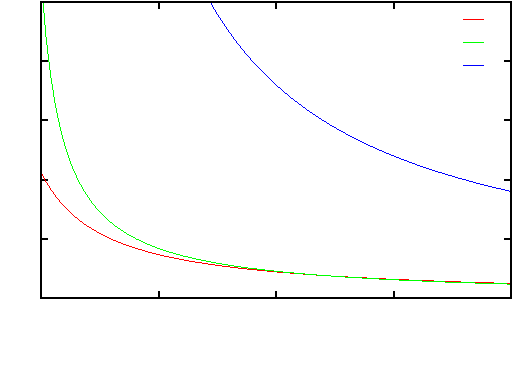
\includegraphics{nucleation_radius}}%
    \gplfronttext
  \end{picture}%
\endgroup
}
%  \label{fig:cnt:critical_number}
%  \subfloat[]{% GNUPLOT: LaTeX picture with Postscript
\begingroup
  \makeatletter
  \providecommand\color[2][]{%
    \GenericError{(gnuplot) \space\space\space\@spaces}{%
      Package color not loaded in conjunction with
      terminal option `colourtext'%
    }{See the gnuplot documentation for explanation.%
    }{Either use 'blacktext' in gnuplot or load the package
      color.sty in LaTeX.}%
    \renewcommand\color[2][]{}%
  }%
  \providecommand\includegraphics[2][]{%
    \GenericError{(gnuplot) \space\space\space\@spaces}{%
      Package graphicx or graphics not loaded%
    }{See the gnuplot documentation for explanation.%
    }{The gnuplot epslatex terminal needs graphicx.sty or graphics.sty.}%
    \renewcommand\includegraphics[2][]{}%
  }%
  \providecommand\rotatebox[2]{#2}%
  \@ifundefined{ifGPcolor}{%
    \newif\ifGPcolor
    \GPcolortrue
  }{}%
  \@ifundefined{ifGPblacktext}{%
    \newif\ifGPblacktext
    \GPblacktexttrue
  }{}%
  % define a \g@addto@macro without @ in the name:
  \let\gplgaddtomacro\g@addto@macro
  % define empty templates for all commands taking text:
  \gdef\gplbacktext{}%
  \gdef\gplfronttext{}%
  \makeatother
  \ifGPblacktext
    % no textcolor at all
    \def\colorrgb#1{}%
    \def\colorgray#1{}%
  \else
    % gray or color?
    \ifGPcolor
      \def\colorrgb#1{\color[rgb]{#1}}%
      \def\colorgray#1{\color[gray]{#1}}%
      \expandafter\def\csname LTw\endcsname{\color{white}}%
      \expandafter\def\csname LTb\endcsname{\color{black}}%
      \expandafter\def\csname LTa\endcsname{\color{black}}%
      \expandafter\def\csname LT0\endcsname{\color[rgb]{1,0,0}}%
      \expandafter\def\csname LT1\endcsname{\color[rgb]{0,1,0}}%
      \expandafter\def\csname LT2\endcsname{\color[rgb]{0,0,1}}%
      \expandafter\def\csname LT3\endcsname{\color[rgb]{1,0,1}}%
      \expandafter\def\csname LT4\endcsname{\color[rgb]{0,1,1}}%
      \expandafter\def\csname LT5\endcsname{\color[rgb]{1,1,0}}%
      \expandafter\def\csname LT6\endcsname{\color[rgb]{0,0,0}}%
      \expandafter\def\csname LT7\endcsname{\color[rgb]{1,0.3,0}}%
      \expandafter\def\csname LT8\endcsname{\color[rgb]{0.5,0.5,0.5}}%
    \else
      % gray
      \def\colorrgb#1{\color{black}}%
      \def\colorgray#1{\color[gray]{#1}}%
      \expandafter\def\csname LTw\endcsname{\color{white}}%
      \expandafter\def\csname LTb\endcsname{\color{black}}%
      \expandafter\def\csname LTa\endcsname{\color{black}}%
      \expandafter\def\csname LT0\endcsname{\color{black}}%
      \expandafter\def\csname LT1\endcsname{\color{black}}%
      \expandafter\def\csname LT2\endcsname{\color{black}}%
      \expandafter\def\csname LT3\endcsname{\color{black}}%
      \expandafter\def\csname LT4\endcsname{\color{black}}%
      \expandafter\def\csname LT5\endcsname{\color{black}}%
      \expandafter\def\csname LT6\endcsname{\color{black}}%
      \expandafter\def\csname LT7\endcsname{\color{black}}%
      \expandafter\def\csname LT8\endcsname{\color{black}}%
    \fi
  \fi
  \setlength{\unitlength}{0.0500bp}%
  \begin{picture}(5040.00,3528.00)%
    \gplgaddtomacro\gplbacktext{%
      \csname LTb\endcsname%
      \put(396,660){\makebox(0,0)[r]{\strut{} 0}}%
      \put(396,1371){\makebox(0,0)[r]{\strut{} 50}}%
      \put(396,2083){\makebox(0,0)[r]{\strut{} 100}}%
      \put(396,2794){\makebox(0,0)[r]{\strut{} 150}}%
      \put(396,3505){\makebox(0,0)[r]{\strut{} 200}}%
      \put(4908,440){\makebox(0,0){\strut{}-2}}%
      \put(3813,440){\makebox(0,0){\strut{}-1.5}}%
      \put(2718,440){\makebox(0,0){\strut{}-1}}%
      \put(1623,440){\makebox(0,0){\strut{}-0.5}}%
      \put(528,440){\makebox(0,0){\strut{} 0}}%
      \put(-374,2082){\rotatebox{90}{\makebox(0,0){\strut{}critical number of molecules}}}%
      \put(2718,110){\makebox(0,0){\strut{}negative pressure (MPa)}}%
    }%
    \gplgaddtomacro\gplfronttext{%
      \csname LTb\endcsname%
      \put(2112,1273){\makebox(0,0)[r]{\strut{}perfluorobutane}}%
      \csname LTb\endcsname%
      \put(2112,1053){\makebox(0,0)[r]{\strut{}perfluoropentane}}%
      \csname LTb\endcsname%
      \put(2112,833){\makebox(0,0)[r]{\strut{}water}}%
    }%
    \gplbacktext
    \put(0,0){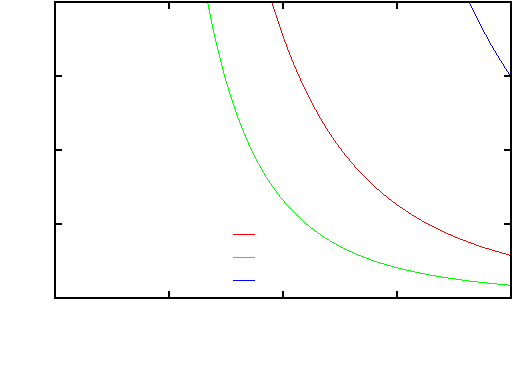
\includegraphics{nucleation_number}}%
    \gplfronttext
  \end{picture}%
\endgroup
}
%  \caption{
%    \Cnt\ predictions for the critical radius and critical number of molecules for a bubble as a function of the pressure.  
%    The vapour is assumed to be an ideal gas, with the vapour pressure obtained by experimental fits to Antoine's equation.
%    The coefficients for Antoine's equation are taken from National Institute of Standards Database\cite{NISTdata}
%    (Note that the perfluorobutane data is used outside of its range of validity, see text).
%  %  The other parameters are taken from the table. \tabref{nuc:parameters}.
%  }
% \label{fig:nucleation_radius}
%\end{figure}
 
%\section{discussion}



%Finally we note that \figref{sppressure} reproduces exactly the result found by Oxtoby\cite{Oxtoby1988}.
%That the vapour spinodal is smaller than the liquid spinodal.
%This was used to explain the difference performance of the classical theory for liquid-bubble cavitation, 
%compared to vapour condensation, (with cavitation doing poorly)




%The final result of the density functional approach, \figref{profile} shows that the thickness of the interface extends over 10 anstrums on each side of the inteface.
%xsThis is extends over most of the bubble wheWhen this compared to the


% \subsection{The density profile}


% For most fluids the interactions are dominated by the strong repulsive forces between the molecules.
% The hard core model is the simplest method of implementing these.
% The pairwise attractive are then treated as a perturbation about the hard core.
% %\begin{align}
% %  F\lrs{\rho(\vr), \rho(\vr^\rpime)} = \fh\lrs{\rho(\vr), \rho(\vr^\rpime)} - \half \phi_{i%j} \rho(\vr_i)\rho(\vr_j)
% %\end{align}
% By writing the joint density $\rho^{(2)} = \rho(\vr)\rho(\vr^\prime)$ we are assuming that there are no correlations in the density distribtution,
% an approximation known as the random phase approximation.

% between most fluids  liquids are well approximated by modelling 
% and so the Free energy can  




% Data for perfluorocarbons in Oh\cite{Oh2010}

%In this chapter we ask the following questions:
%\nlist{
%  \item What is the critical radius of a bubble as a function of pressure.
%  \item At what pressures do we expect the perfluorocarbon oils undergo type 1 nucleation? \label{item:nuc_question1}
 % \item Can the perfluorocarbons be mixed in order to tune the nucleation pressure?\label{item:nuc_question2}
%}
%To answer these questions we need to calculate the  rate of nucleation.
%The bulk of this chapter is dedicated to calculating these rates; first as a function of pressure,
%and second as a function of the perfluorocarbon mixing.
%\todo{get rid of wishful thinking}


%This chapter calculates the pressures required to cavitate perfluorobutane and perfluoropentane
%by using \cnt.
%This is done with classical nucleation theo
% In this chapter we ask At what pressures do we expect the perfluorocarbon oils undergo type 1 nucleation?the following questions:
% \nlist{
%   \item At what pressures do we expect the perfluorocarbon oils undergo type 1 nucleation? \label{item:nuc_question1}
%   \item Can the perfluorocarbons be mixed in order to tune the nucleation pressure?\label{item:nuc_question2}
% }
% To answer these questions we need to calculate the  rate of nucleation.
% The bulk of this chapter is dedicated to calculating these rates; first as a function of pressure,
% and second a
%%%
%
%Theoretical rate calculations areThe nucleation rate has 
%%
%
%he simplest estimate for nucleation rate is provided by  \cnt, which is discussed in \secref{nuc:CNT}.
%This method is essentially an application of the Aarenhius equation.
%The energy barrier to nucleation is found from thermodynamic arguments,
%while the rate is obtained from a kinematic argument.


\subsection{Testing the validity of the capillary approximation}\label{sec:nuc:DFT}
%\begin{quote}
%  An enthusiastic graduate student ... has heard that the density functional approach is {\em the} thing to use but is confused by the plethora of possible approximations.
%Which recipe or recipes do you recommend?  This would be my advice.
%The simple van der Waals approximation is always a good starting point.
%\flushright{Evans}
%\end{quote}
%From \cite{Oxtoby1992}


%\subsubsection{Introduction}

For small bubbles, the assumption of a sharp interface between the bubble and its medium is open to criticism.
Can the width of the interface really be insignificant for a bubble \unit{50}\nano\metre\ wide?
In this section we investigate the issue by taking an alternative approach,
the density functional programme of Oxtoby and Evans\cite{Oxtoby1988}.
%more carefully modelling the interactions at the interface.
%This is done by following the density functional programme of Oxtoby and Evans\cite{Oxtoby1988}.


\Dft\ relaxes the capillary approximation used in \cnt.
The density of the nucleated bubble is not assumed to be uniform,
and the interface is not assumed to be macroscopic and plainer\cite{Oxtoby1992, Oxtoby1988}.
The density functional approach therefore does much better at modelling the interface than \cnt.
Rather than it being a sharp boundary,
there is a finite interval over which the density varies from that of the fluid to that of the vapour.
%However, the density functional approach also models the change in  density across liquid-vapour interface,
%whence removing the flawed capillary approximation from the calculation.
In addition, and as will be shown, the energy barrier to the phase change vanishes at the spinodal.
This is as it should be, but marks a second major improvement on the classical theory\cite{Talanquer1997}.



%and the bubble is modelled for what it is -  a fluctuation in density - 
%rather than a vapour entrapped in  flexible boundary.

%Here we use density functional theory only test the approximations of the classical calculations already carried.
%Density functional theory can be us to calculate the nucleation rate.
%However, it approaches the problem microscopically from a model for the intermolecular potential.
%The calculated rate is, just as in the classical case, exceptionally sensitive to the parameters fed to this model.
%To make quantitative predictions  a semi-empirical approach can be used that fits the parameters to the bulk properties of the fluid\cite{Nyquist1995}.
%Unfortunately, however,  perfluoropentane does not have sufficient data for either the density variations with temperature 
%or the chemical potential variations with temperature.

%This makes qantative predictions unlikeThe vapour pressure 

%\begin{figure}
%  % GNUPLOT: LaTeX picture with Postscript
\begingroup
  \makeatletter
  \providecommand\color[2][]{%
    \GenericError{(gnuplot) \space\space\space\@spaces}{%
      Package color not loaded in conjunction with
      terminal option `colourtext'%
    }{See the gnuplot documentation for explanation.%
    }{Either use 'blacktext' in gnuplot or load the package
      color.sty in LaTeX.}%
    \renewcommand\color[2][]{}%
  }%
  \providecommand\includegraphics[2][]{%
    \GenericError{(gnuplot) \space\space\space\@spaces}{%
      Package graphicx or graphics not loaded%
    }{See the gnuplot documentation for explanation.%
    }{The gnuplot epslatex terminal needs graphicx.sty or graphics.sty.}%
    \renewcommand\includegraphics[2][]{}%
  }%
  \providecommand\rotatebox[2]{#2}%
  \@ifundefined{ifGPcolor}{%
    \newif\ifGPcolor
    \GPcolorfalse
  }{}%
  \@ifundefined{ifGPblacktext}{%
    \newif\ifGPblacktext
    \GPblacktexttrue
  }{}%
  % define a \g@addto@macro without @ in the name:
  \let\gplgaddtomacro\g@addto@macro
  % define empty templates for all commands taking text:
  \gdef\gplbacktext{}%
  \gdef\gplfronttext{}%
  \makeatother
  \ifGPblacktext
    % no textcolor at all
    \def\colorrgb#1{}%
    \def\colorgray#1{}%
  \else
    % gray or color?
    \ifGPcolor
      \def\colorrgb#1{\color[rgb]{#1}}%
      \def\colorgray#1{\color[gray]{#1}}%
      \expandafter\def\csname LTw\endcsname{\color{white}}%
      \expandafter\def\csname LTb\endcsname{\color{black}}%
      \expandafter\def\csname LTa\endcsname{\color{black}}%
      \expandafter\def\csname LT0\endcsname{\color[rgb]{1,0,0}}%
      \expandafter\def\csname LT1\endcsname{\color[rgb]{0,1,0}}%
      \expandafter\def\csname LT2\endcsname{\color[rgb]{0,0,1}}%
      \expandafter\def\csname LT3\endcsname{\color[rgb]{1,0,1}}%
      \expandafter\def\csname LT4\endcsname{\color[rgb]{0,1,1}}%
      \expandafter\def\csname LT5\endcsname{\color[rgb]{1,1,0}}%
      \expandafter\def\csname LT6\endcsname{\color[rgb]{0,0,0}}%
      \expandafter\def\csname LT7\endcsname{\color[rgb]{1,0.3,0}}%
      \expandafter\def\csname LT8\endcsname{\color[rgb]{0.5,0.5,0.5}}%
    \else
      % gray
      \def\colorrgb#1{\color{black}}%
      \def\colorgray#1{\color[gray]{#1}}%
      \expandafter\def\csname LTw\endcsname{\color{white}}%
      \expandafter\def\csname LTb\endcsname{\color{black}}%
      \expandafter\def\csname LTa\endcsname{\color{black}}%
      \expandafter\def\csname LT0\endcsname{\color{black}}%
      \expandafter\def\csname LT1\endcsname{\color{black}}%
      \expandafter\def\csname LT2\endcsname{\color{black}}%
      \expandafter\def\csname LT3\endcsname{\color{black}}%
      \expandafter\def\csname LT4\endcsname{\color{black}}%
      \expandafter\def\csname LT5\endcsname{\color{black}}%
      \expandafter\def\csname LT6\endcsname{\color{black}}%
      \expandafter\def\csname LT7\endcsname{\color{black}}%
      \expandafter\def\csname LT8\endcsname{\color{black}}%
    \fi
  \fi
  \setlength{\unitlength}{0.0500bp}%
  \begin{picture}(5040.00,3528.00)%
    \gplgaddtomacro\gplbacktext{%
      \csname LTb\endcsname%
      \put(1210,704){\makebox(0,0)[r]{\strut{} 0}}%
      \put(1210,1070){\makebox(0,0)[r]{\strut{} 0.5}}%
      \put(1210,1435){\makebox(0,0)[r]{\strut{} 1}}%
      \put(1210,1801){\makebox(0,0)[r]{\strut{} 1.5}}%
      \put(1210,2167){\makebox(0,0)[r]{\strut{} 2}}%
      \put(1210,2533){\makebox(0,0)[r]{\strut{} 2.5}}%
      \put(1210,2898){\makebox(0,0)[r]{\strut{} 3}}%
      \put(1210,3264){\makebox(0,0)[r]{\strut{} 3.5}}%
      \put(1342,484){\makebox(0,0){\strut{} 200}}%
      \put(1791,484){\makebox(0,0){\strut{} 220}}%
      \put(2240,484){\makebox(0,0){\strut{} 240}}%
      \put(2689,484){\makebox(0,0){\strut{} 260}}%
      \put(3138,484){\makebox(0,0){\strut{} 280}}%
      \put(3587,484){\makebox(0,0){\strut{} 300}}%
      \put(4036,484){\makebox(0,0){\strut{} 320}}%
      \put(4485,484){\makebox(0,0){\strut{} 340}}%
      \put(440,1984){\rotatebox{90}{\makebox(0,0){\strut{}vapour pressure, atm}}}%
      \put(3026,154){\makebox(0,0){\strut{}temperature, K}}%
    }%
    \gplgaddtomacro\gplfronttext{%
      \csname LTb\endcsname%
      \put(3058,3091){\makebox(0,0)[r]{\strut{}fit}}%
      \csname LTb\endcsname%
      \put(3058,2871){\makebox(0,0)[r]{\strut{}Barber 1955}}%
      \csname LTb\endcsname%
      \put(3058,2651){\makebox(0,0)[r]{\strut{}Crowder 1967}}%
    }%
    \gplbacktext
    \put(0,0){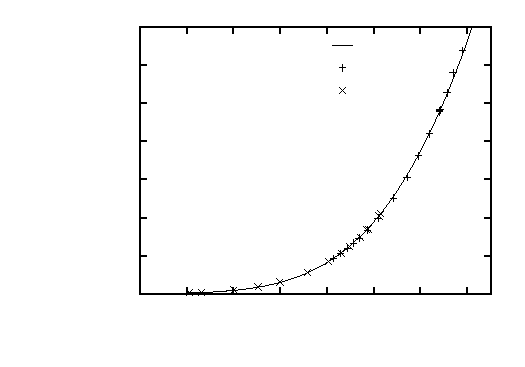
\includegraphics{c2_vapour_pressure_fit}}%
    \gplfronttext
  \end{picture}%
\endgroup

%  \caption{ Fitting the Lennard-Jones model to experimental data for the vapour pressure of perfluoropentane\cite{NISTdata}.
%   However, there is insufficient density data available for perfluoropentane to constrain the data for quantitative measurements.    
%  }
% \label{fig:vapour_pressure}
%\end{figure}
%Data does exist for the vapour pressure as a function of temperature.
%This is used with the single datum  for the density at room temperature to fit the model.
%The result of the fit given in \figref{vapour_pressure}.
%However, enough confidence cannot be placed in the fits to use for quantitative predictions. 
% To use density functional theory toe 

% To calculate the nucleation rate the  Arrhenius form of \eqnref{} is still used.
% The prefactor $J_0$ also remains the same.
% The removal of the capillary approximation changes the expression of the free-energy
% in the exponential.
% It is this quantity that we wish to calculate.

% Rather than starting with thermodynamics, \Dft\ approaches the problem microscopically
 \Dft\ starts by modelling the inter-molecular potentials.
 Good models for the fluid potential exist and 
 among the most widely used are the Lennard-Jones potential
 and the Kihira potential.
 The former describes small spherically symmetric molecules very accurately.
 The latter is a extension on the Lennard-Jones model to describe larger, less symmetric molecules.


In principle, macroscopic predictions can then be drawn by inserting the intermolecular potentials into the usual thermodynamic potentials of statistical mechanics.  
While the full multi-particle potentials are in general insolvable and approximations must be made,
the density functional approach is one derived from a firm theoretical base\cite{Evans1992}.
%the data inputted does not need to be provided.
Unfortunately, when applied to nucleation, the first principles approach  has only ever had qualitative success\cite{Nyquist1995,Talanquer2001},
with the predictions being very sensitive to the modelled molecular scale parameters.
%The nucleation rates still depend exponentially on the predicted energy barrier and small deviations have a profound influence on predictions.
%and the success of the density functional approach to nucleation - without the empirical input - has always only been qualitative

The semi-empirical approach of Nyquist\cite{Nyquist1995} and Talanquer\cite{Talanquer2001}
attempts to temper this sensitivity by fitting the molecular-scale parameters to the experimental data used for the classical theory.
% to making nucleation rate predictions.
% By construction, therefore, the bulk predications of the model are correct. 
By construction, therefore, the bulk thermodynamic predications of the model are correct.
Thermodynamic arguments can then be used to obtain other quantities of interest, such as the nucleation rate. 
We shall use this approach to test the width of interface between the bubble and its medium.
% such as those in equation \eqnref{}.


 %However, by modelling the change in  density across liquid-vapour interface,
 %one of the major flaws of the capillary approximation is removed.
 %In addition with this approach, the energy barrier to the phase change vanishes at the spinodal,
 %a second major correction on the classical theory.


The density functional approach models fluctuations about the bulk properties of the fluid.
It is therefore a mean-field approach that fails, like all mean field theories, near to the critical temperature.
One must be cautious, therefore, only to apply it to nucleation events that occur well away from the critical point.
In this thesis  attention is restricted to nucleation events that are induced by a reduction in pressure 
rather than by boiling.
The critical temperatures for a number of perfluorocarbons are listed in \tabref{nuc:criticalTemps}.
It is interesting to note that for the perfluorocarbons the critical temperatures are considerably higher than their boiling points.
At \unit{37}\degreecelsius, for example, perfluoropentane is in a meta-stable state but is still far from being `on the cusp' of vapourisation.
Type 1 nucleation events are still likely to occur via a reduction in pressure rather than an increase in temperature.
On the other hand, perfluoroethane is above its  critical point at room temperature and we 
consider it to be a little to close to its  critical point to be considered in this thesis.

% The oil chosen for this purpose is perfluoropentane.
% It has the following properties that make it suitable
% \nlist{
% \item
%   it is chemically inert with a low toxicity, \label{nuc:PFP:one} \todo{some references here} 
% \item
%   it has a boiling point of about \unit{28}\degreecelsius. \label{nuc:PFP:two}\todo{some references here to} 
% }
% Property \ref{nuc:PFP:one} is important for any diagnostic contrast agent.
% Property \ref{nuc:PFP:two} suggests that when placed under tension
% \pfp\ should vapourise  more readily than the bulk (assumed to be water).
% This would then give the required selectivity for the contrast agent.
% %It is an oversimplification, however, 
% %to argue that  \pfp's lower boiling point implies that it should form bubbles prior to the bulk.
% %There are multiple mechanisms to bubble nucleation in ultrasound.
% %We argue in \secref{} that the mechanisms for water and \pfp\ droplets are likely to be different,
% %and that the boiling point in the case of water   is not relevant in diagnostic cavitation.

% making a comparison based on the respective physical chemistry incorrect.



%and are then used to derive further
%  so that the model reproduces the 
%correct thermodynamic limit.
%
%While \cnt\ is a useful first calculation,
%it is not adequate to provide quantitative  predictions.
%To overcome these difficulties we employ the semi-empirical density functional approach of Nyquist\cite{Nyquist1995} and Talanquer\cite{Talanquer2001}
%in \secref{nuc:DFT}.
%The {\em semi-empirical} approach uses the same 
%By construction, therefore, the bulk predications of the model are correct. 



% The density functional approach calculates  the free energy 
% directly from the interaction potentials.
% However, as for the classical theory,
% the calculated rates are exponentially sensitive to inaccuracies in the provided model.
% Great care must be taken, therefore, when setting up the models.

% The semi-empiciral approach ...
% Fits so that in the bulk limit...
% DFT then proposes the  details omitted by the classical theory,
% such as finite with of interface.


% Use the approach of Nyquist to calcualate the rate of perlfuorpentane and perfluorbutane.
\subsubsection{Outline of approach}
The approach we will be taking can be summarised as follows:
%In short, the algorithm we shall be using proceeds as follows % The steps that are to be taken are 
 \nlist{
   \item write down an accurate model for the intermolecular potential (\secref{nuc:DFT:write}),
   \item approximate the model so that it can be solved (\secref{nuc:DFT:approx}),
   \item fit the model's parameters so that it reproduces macroscopic thermodynamics (\secref{nuc:DFT:fit}),
   \item predict the shape of the interface between the bubble and its medium and compare it with the capillary approximation (\secref{nuc:DFT:results}).
 }



\subsubsection{The density functional approach}\label{sec:nuc:DFT:write}

The density functional approach is a statistical theory 
that attempts to model the grand potential, $\Omega$,
at a molecular level.
% in \eqnref{nuc:astarR} %is required to evaluate both the rate of nucleation and the critical radius.
%If  spherical symmetry is assumed then 
%the bubble boundary is defined by its radius.
%The critical radius is such that\cite{Oxtoby1992,Oxtoby1988}
%\begin{align}
%  \frac{d \Omega}{d a} =0,\quad\text{at $a = \astar$} \label{eqn:DFT:astarR}
%\end{align}
%where $\Omega$ is the {\em grand potential}.
%
%
%is difficult to evaluate on a microscopic level, however, the grand potential 
The exact solution is intractable due to the mutual interactions between every molecule in the system.
%because it depends upon the free energy, 
%which in turn It is difficult to evaluate
%because the positions of the molecules within the system are not independent,
%but rather depend on the position of every other molecule due to their mutual interactions.
%This is because 
%the intrinsic free energy incorporates the interaction of every molecule with every other molecule in the system.
%Evaluating the intrinsic free energy is then intractable.
%This introduces integrals that are intractable.
%The approach of \dft\ to this problem is standard in statistical physics:

To overcome this problem 
the true probability density function, $p_0(\H; \cx_1,\cp_1)$, that describes 
the positions of the particles and their momenta,
is approximated to a simpler distribution $p(H; \cx_1, \cp_1)$ that may be solved.
Here, $\H$, is the true Hamiltonian of the system 
and $H$ is the approximate Hamiltonian with simpler interaction terms.
We have also employed the  convenient shorthand
\begin{align}
\cx_n \equiv r_n,r_{n+1},\ldots,r_N,  \quad\text{and}\quad
\cp_n \equiv  p_n,p_{n+1},\ldots, p_N.
    \label{eqn:shorthand}
\end{align}
to describe the positions and momenta of  $N-n$ particles.

The {\em relative entropy } or {\em Kullback-Leibler divergance} gives the amount of information lost 
when using the approximate distribution  $p$ rather than the correct distribution $p_0$,
and is defined
\begin{align}
  \KLD{p}{p_0} = \Tr p \log \frac{p}{p_0}, \label{eqn:nuc:KLD}
\end{align}
where $\Tr$ is the classical trace operator. %$\Tr\equiv \sum_{N=0}^\infty \frac{1}{h^{3N}N!} \iint d\cx_1 d\cp_1$ is the classical trace operator.
The relative entropy has the property that 
$\KLD{p}{p_0} \ge 0$, which follows from Gibbs inequality\cite{MacKayBook}.
Only if $p=p_0$ does $\KLD{p}{p_0} = 0$.
Therefore, once the structure of the approximate  distribution $p$ has been chosen,
it can be varied to match to content of $p_0$ as closely as possible by minimising $\KLD{p}{p_0}$.
% In this thesis we consider only pair-wise interactions,
% \begin{align}
% %  \UE(\cx) \approx 
% \Phi(\cx) =  \sum_{j>i} \sum_i^N \phi(\vr_i, \vr_j),
% \end{align}
% where $\phi(\vr_i, \vr_j)$ is the two particle potential between a particle at $r_i$ and $r_j$.
% The structure imposed by higher-order correlations  is ignored by $p$.

Employing this variational procedure to approximate the thermodynamic potentials is ubiquitous in statistical physics\cite{Yedidia2000a}.
The point of departure for the density functional method is the realisation that
\nlist{
\item the {\em density is a functional of the external potential.}
  This follows because the approximation to the  density is related to the single particle probability density function
  \begin{align}
    \rho(\vr) \propto \iint d\cp_1 d\cx_2 p(H, \cx, \cp) \propto  \int e^{-\beta\sum_i^N V_\ext(\vr_i)} d\cx_2
  \end{align}
  where $V_\ext(\vr_i)$ is the external potential at the position $\vr$ of the $i^{th}$ molecule.
  Here were have extended the shorthand  employed in  \eqnref{dshorthand} so that
  \begin{align}
    d\cx_n &\equiv dr_n dr_{n+1}\ldots dr_N, &&\quad\text{and}&
    d\cp_n &\equiv  dp_n dp_{n+1}\ldots dp_N.
    \label{eqn:dshorthand}
  \end{align}
\item {\em the external potential is uniquely determined by the density}.
  This converse result is known as the Hohenberg-Kohn theorem.
%  and an outline of the proof is given in  \appref{DFT}.
  It follows because the external potential is determined by the probability density, $p$, which is in turn determined uniquely by the density.
}
It is thereby permissible to work with the mass density rather than the probability density when considering the thermodynamics of the bubble.
Since the density is the term of interest, the density functional approach is much more direct.
We may therefore define a approximate grand potential, $\Omega_V$, as a functional of the (approximate) density \cite{Evans1992},
\begin{align}
 \Omega_V\lrs{\rho} \equiv \beta^{-1}\KLD{p\lrs{\rho}}{p_0}+   \Omega. 
\end{align}
The approximate  grand potential approaches the true value when
it is minimised with  respect to $\rho$.
Furthermore, since $\Omega$ is the grand potential at thermodynamic equilibrium,
$\Omega_V$ is minimal when $\rho$ describes the  critical density distribution.
The condition of equation \eqnref{nuc:astarR}
can therefore be expressed by the functional derivative\cite{Oxtoby1992}
\begin{align}
  \frac{\delta \Omega_V}{\delta \rho} =0,\quad\text{at $\rho = \rhostar$.} \label{eqn:DFT:astar}
\end{align}


%\subsubsection{The critical bubble}
The grand potential is related to the Helmholtz free energy by a Legendre transformation
\begin{align}
  \Omega_V = F -  \mu \int d\vr \rho(\vr), \label{eqn:OmegaVDefn}
\end{align}
where $\mu$ is the chemical potential.
%The chemical potential is comprised of the two phases of a nucleating bubble:
%the oil and its vapour.
The free energy, $F$, is the sum of  internal energy $\Phi$ and an  entropic contribution.
The inter-particle interactions are contained within the internal energy.

\subsubsection{Approximate the model}\label{sec:nuc:DFT:approx}
To simplify $F$ it is noted that  the interactions of most fluids are dominated  by volume exclusion effects (van der Waal type interactions).
Longer range interactions are, in general, only of secondary importance\cite{Oxtoby1992}.
If only pair-wise attractions are considered, then the internal energy can then be split into the 
free energy of a {\em hard sphere} reference fluid, $F_\hs$ 
and a small perturbation, $\phi_\attr$, that incorporates the long range attractions.
Then 
\begin{align}
   F\lrs{\rho} = F_\hs\lrs{\rho} +\half   \iint d \vr_i d\vr_j \phi_\attr( \vr_i, \vr_j)\rho(\vr_i, \vr_j),  \label{eqn:F_pert}
\end{align}
where $\phi_\attr(\vr_i, \vr_j)$ is the residual two particle potential between a particle at $\vr_i$ and $\vr_j$,
not incorporated into $F_\hs$.
$\rho(\vr_i, \vr_j) $ is the two particle density function.
(See Evans\cite{Evans1992} for a formal treatment of the above steps).

% \begin{figure}
%  \centering
% %\hspace*{-0.2cm}
%  \label{fig:Kihira_potentials}
%  \subfloat[Kihira 2-particle potentials for various perfluorocarbons]{
%   % GNUPLOT: LaTeX picture with Postscript
\begingroup
  \makeatletter
  \providecommand\color[2][]{%
    \GenericError{(gnuplot) \space\space\space\@spaces}{%
      Package color not loaded in conjunction with
      terminal option `colourtext'%
    }{See the gnuplot documentation for explanation.%
    }{Either use 'blacktext' in gnuplot or load the package
      color.sty in LaTeX.}%
    \renewcommand\color[2][]{}%
  }%
  \providecommand\includegraphics[2][]{%
    \GenericError{(gnuplot) \space\space\space\@spaces}{%
      Package graphicx or graphics not loaded%
    }{See the gnuplot documentation for explanation.%
    }{The gnuplot epslatex terminal needs graphicx.sty or graphics.sty.}%
    \renewcommand\includegraphics[2][]{}%
  }%
  \providecommand\rotatebox[2]{#2}%
  \@ifundefined{ifGPcolor}{%
    \newif\ifGPcolor
    \GPcolortrue
  }{}%
  \@ifundefined{ifGPblacktext}{%
    \newif\ifGPblacktext
    \GPblacktexttrue
  }{}%
  % define a \g@addto@macro without @ in the name:
  \let\gplgaddtomacro\g@addto@macro
  % define empty templates for all commands taking text:
  \gdef\gplbacktext{}%
  \gdef\gplfronttext{}%
  \makeatother
  \ifGPblacktext
    % no textcolor at all
    \def\colorrgb#1{}%
    \def\colorgray#1{}%
  \else
    % gray or color?
    \ifGPcolor
      \def\colorrgb#1{\color[rgb]{#1}}%
      \def\colorgray#1{\color[gray]{#1}}%
      \expandafter\def\csname LTw\endcsname{\color{white}}%
      \expandafter\def\csname LTb\endcsname{\color{black}}%
      \expandafter\def\csname LTa\endcsname{\color{black}}%
      \expandafter\def\csname LT0\endcsname{\color[rgb]{1,0,0}}%
      \expandafter\def\csname LT1\endcsname{\color[rgb]{0,1,0}}%
      \expandafter\def\csname LT2\endcsname{\color[rgb]{0,0,1}}%
      \expandafter\def\csname LT3\endcsname{\color[rgb]{1,0,1}}%
      \expandafter\def\csname LT4\endcsname{\color[rgb]{0,1,1}}%
      \expandafter\def\csname LT5\endcsname{\color[rgb]{1,1,0}}%
      \expandafter\def\csname LT6\endcsname{\color[rgb]{0,0,0}}%
      \expandafter\def\csname LT7\endcsname{\color[rgb]{1,0.3,0}}%
      \expandafter\def\csname LT8\endcsname{\color[rgb]{0.5,0.5,0.5}}%
    \else
      % gray
      \def\colorrgb#1{\color{black}}%
      \def\colorgray#1{\color[gray]{#1}}%
      \expandafter\def\csname LTw\endcsname{\color{white}}%
      \expandafter\def\csname LTb\endcsname{\color{black}}%
      \expandafter\def\csname LTa\endcsname{\color{black}}%
      \expandafter\def\csname LT0\endcsname{\color{black}}%
      \expandafter\def\csname LT1\endcsname{\color{black}}%
      \expandafter\def\csname LT2\endcsname{\color{black}}%
      \expandafter\def\csname LT3\endcsname{\color{black}}%
      \expandafter\def\csname LT4\endcsname{\color{black}}%
      \expandafter\def\csname LT5\endcsname{\color{black}}%
      \expandafter\def\csname LT6\endcsname{\color{black}}%
      \expandafter\def\csname LT7\endcsname{\color{black}}%
      \expandafter\def\csname LT8\endcsname{\color{black}}%
    \fi
  \fi
  \setlength{\unitlength}{0.0500bp}%
  \begin{picture}(3276.00,3276.00)%
    \gplgaddtomacro\gplbacktext{%
      \csname LTb\endcsname%
      \put(341,660){\makebox(0,0)[r]{\strut{}-800}}%
      \put(341,1092){\makebox(0,0)[r]{\strut{}-600}}%
      \put(341,1524){\makebox(0,0)[r]{\strut{}-400}}%
      \put(341,1957){\makebox(0,0)[r]{\strut{}-200}}%
      \put(341,2389){\makebox(0,0)[r]{\strut{} 0}}%
      \put(341,2821){\makebox(0,0)[r]{\strut{} 200}}%
      \put(341,3253){\makebox(0,0)[r]{\strut{} 400}}%
      \put(732,440){\makebox(0,0){\strut{} 6}}%
      \put(1251,440){\makebox(0,0){\strut{} 8}}%
      \put(1770,440){\makebox(0,0){\strut{} 10}}%
      \put(2289,440){\makebox(0,0){\strut{} 12}}%
      \put(2808,440){\makebox(0,0){\strut{} 14}}%
      \put(-165,1956){\rotatebox{90}{\makebox(0,0){\strut{}  $\Phi(r)$ (K)}}}%
      \put(1770,110){\makebox(0,0){\strut{}distance ({\AA })}}%
    }%
    \gplgaddtomacro\gplfronttext{%
      \csname LTb\endcsname%
      \put(2476,3080){\makebox(0,0)[r]{\strut{}$C_4F_{10}-C_4F_{10}$}}%
      \csname LTb\endcsname%
      \put(2476,2860){\makebox(0,0)[r]{\strut{}$C_5F_{12}-C_5F_{12}$}}%
      \csname LTb\endcsname%
      \put(2476,2640){\makebox(0,0)[r]{\strut{}$C_6F_{14}-C_6F_{14}$}}%
    }%
    \gplbacktext
    \put(0,0){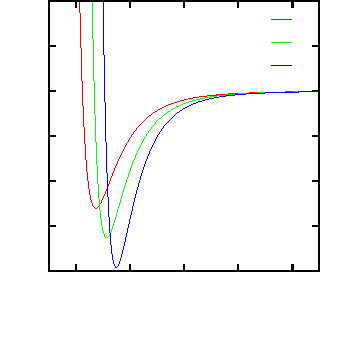
\includegraphics{c2_plot_potentials}}%
    \gplfronttext
  \end{picture}%
\endgroup
}
% \hfill
%  \label{fig:Kihira_WCA}
%  \subfloat[WCA decomposition of the Kihira  potential for perfluoropentane]{
%   % GNUPLOT: LaTeX picture with Postscript
\begingroup
  \makeatletter
  \providecommand\color[2][]{%
    \GenericError{(gnuplot) \space\space\space\@spaces}{%
      Package color not loaded in conjunction with
      terminal option `colourtext'%
    }{See the gnuplot documentation for explanation.%
    }{Either use 'blacktext' in gnuplot or load the package
      color.sty in LaTeX.}%
    \renewcommand\color[2][]{}%
  }%
  \providecommand\includegraphics[2][]{%
    \GenericError{(gnuplot) \space\space\space\@spaces}{%
      Package graphicx or graphics not loaded%
    }{See the gnuplot documentation for explanation.%
    }{The gnuplot epslatex terminal needs graphicx.sty or graphics.sty.}%
    \renewcommand\includegraphics[2][]{}%
  }%
  \providecommand\rotatebox[2]{#2}%
  \@ifundefined{ifGPcolor}{%
    \newif\ifGPcolor
    \GPcolortrue
  }{}%
  \@ifundefined{ifGPblacktext}{%
    \newif\ifGPblacktext
    \GPblacktexttrue
  }{}%
  % define a \g@addto@macro without @ in the name:
  \let\gplgaddtomacro\g@addto@macro
  % define empty templates for all commands taking text:
  \gdef\gplbacktext{}%
  \gdef\gplfronttext{}%
  \makeatother
  \ifGPblacktext
    % no textcolor at all
    \def\colorrgb#1{}%
    \def\colorgray#1{}%
  \else
    % gray or color?
    \ifGPcolor
      \def\colorrgb#1{\color[rgb]{#1}}%
      \def\colorgray#1{\color[gray]{#1}}%
      \expandafter\def\csname LTw\endcsname{\color{white}}%
      \expandafter\def\csname LTb\endcsname{\color{black}}%
      \expandafter\def\csname LTa\endcsname{\color{black}}%
      \expandafter\def\csname LT0\endcsname{\color[rgb]{1,0,0}}%
      \expandafter\def\csname LT1\endcsname{\color[rgb]{0,1,0}}%
      \expandafter\def\csname LT2\endcsname{\color[rgb]{0,0,1}}%
      \expandafter\def\csname LT3\endcsname{\color[rgb]{1,0,1}}%
      \expandafter\def\csname LT4\endcsname{\color[rgb]{0,1,1}}%
      \expandafter\def\csname LT5\endcsname{\color[rgb]{1,1,0}}%
      \expandafter\def\csname LT6\endcsname{\color[rgb]{0,0,0}}%
      \expandafter\def\csname LT7\endcsname{\color[rgb]{1,0.3,0}}%
      \expandafter\def\csname LT8\endcsname{\color[rgb]{0.5,0.5,0.5}}%
    \else
      % gray
      \def\colorrgb#1{\color{black}}%
      \def\colorgray#1{\color[gray]{#1}}%
      \expandafter\def\csname LTw\endcsname{\color{white}}%
      \expandafter\def\csname LTb\endcsname{\color{black}}%
      \expandafter\def\csname LTa\endcsname{\color{black}}%
      \expandafter\def\csname LT0\endcsname{\color{black}}%
      \expandafter\def\csname LT1\endcsname{\color{black}}%
      \expandafter\def\csname LT2\endcsname{\color{black}}%
      \expandafter\def\csname LT3\endcsname{\color{black}}%
      \expandafter\def\csname LT4\endcsname{\color{black}}%
      \expandafter\def\csname LT5\endcsname{\color{black}}%
      \expandafter\def\csname LT6\endcsname{\color{black}}%
      \expandafter\def\csname LT7\endcsname{\color{black}}%
      \expandafter\def\csname LT8\endcsname{\color{black}}%
    \fi
  \fi
  \setlength{\unitlength}{0.0500bp}%
  \begin{picture}(3276.00,3276.00)%
    \gplgaddtomacro\gplbacktext{%
      \csname LTb\endcsname%
      \put(473,660){\makebox(0,0)[r]{\strut{}-800}}%
      \put(473,1092){\makebox(0,0)[r]{\strut{}-600}}%
      \put(473,1524){\makebox(0,0)[r]{\strut{}-400}}%
      \put(473,1957){\makebox(0,0)[r]{\strut{}-200}}%
      \put(473,2389){\makebox(0,0)[r]{\strut{} 0}}%
      \put(473,2821){\makebox(0,0)[r]{\strut{} 200}}%
      \put(473,3253){\makebox(0,0)[r]{\strut{} 400}}%
      \put(605,440){\makebox(0,0){\strut{} 2}}%
      \put(1004,440){\makebox(0,0){\strut{} 4}}%
      \put(1403,440){\makebox(0,0){\strut{} 6}}%
      \put(1802,440){\makebox(0,0){\strut{} 8}}%
      \put(2201,440){\makebox(0,0){\strut{} 10}}%
      \put(2600,440){\makebox(0,0){\strut{} 12}}%
      \put(2999,440){\makebox(0,0){\strut{} 14}}%
      \put(-33,1956){\rotatebox{90}{\makebox(0,0){\strut{}  $\Phi(r)$ (K)}}}%
      \put(1902,110){\makebox(0,0){\strut{}distance ({\AA })}}%
    }%
    \gplgaddtomacro\gplfronttext{%
      \csname LTb\endcsname%
      \put(2608,3080){\makebox(0,0)[r]{\strut{}repulsive}}%
      \csname LTb\endcsname%
      \put(2608,2860){\makebox(0,0)[r]{\strut{}attractive}}%
    }%
    \gplbacktext
    \put(0,0){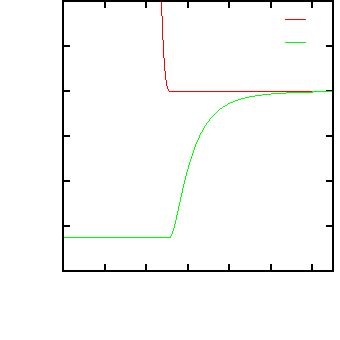
\includegraphics{c2_plot_potentials_WCA}}%
    \gplfronttext
  \end{picture}%
\endgroup
}\\
% \label{fig:Kihira_d}
% \subfloat[Comparison of the WCA repulsive potential with the hard sphere potential]{
%   % GNUPLOT: LaTeX picture with Postscript
\begingroup
  \makeatletter
  \providecommand\color[2][]{%
    \GenericError{(gnuplot) \space\space\space\@spaces}{%
      Package color not loaded in conjunction with
      terminal option `colourtext'%
    }{See the gnuplot documentation for explanation.%
    }{Either use 'blacktext' in gnuplot or load the package
      color.sty in LaTeX.}%
    \renewcommand\color[2][]{}%
  }%
  \providecommand\includegraphics[2][]{%
    \GenericError{(gnuplot) \space\space\space\@spaces}{%
      Package graphicx or graphics not loaded%
    }{See the gnuplot documentation for explanation.%
    }{The gnuplot epslatex terminal needs graphicx.sty or graphics.sty.}%
    \renewcommand\includegraphics[2][]{}%
  }%
  \providecommand\rotatebox[2]{#2}%
  \@ifundefined{ifGPcolor}{%
    \newif\ifGPcolor
    \GPcolortrue
  }{}%
  \@ifundefined{ifGPblacktext}{%
    \newif\ifGPblacktext
    \GPblacktexttrue
  }{}%
  % define a \g@addto@macro without @ in the name:
  \let\gplgaddtomacro\g@addto@macro
  % define empty templates for all commands taking text:
  \gdef\gplbacktext{}%
  \gdef\gplfronttext{}%
  \makeatother
  \ifGPblacktext
    % no textcolor at all
    \def\colorrgb#1{}%
    \def\colorgray#1{}%
  \else
    % gray or color?
    \ifGPcolor
      \def\colorrgb#1{\color[rgb]{#1}}%
      \def\colorgray#1{\color[gray]{#1}}%
      \expandafter\def\csname LTw\endcsname{\color{white}}%
      \expandafter\def\csname LTb\endcsname{\color{black}}%
      \expandafter\def\csname LTa\endcsname{\color{black}}%
      \expandafter\def\csname LT0\endcsname{\color[rgb]{1,0,0}}%
      \expandafter\def\csname LT1\endcsname{\color[rgb]{0,1,0}}%
      \expandafter\def\csname LT2\endcsname{\color[rgb]{0,0,1}}%
      \expandafter\def\csname LT3\endcsname{\color[rgb]{1,0,1}}%
      \expandafter\def\csname LT4\endcsname{\color[rgb]{0,1,1}}%
      \expandafter\def\csname LT5\endcsname{\color[rgb]{1,1,0}}%
      \expandafter\def\csname LT6\endcsname{\color[rgb]{0,0,0}}%
      \expandafter\def\csname LT7\endcsname{\color[rgb]{1,0.3,0}}%
      \expandafter\def\csname LT8\endcsname{\color[rgb]{0.5,0.5,0.5}}%
    \else
      % gray
      \def\colorrgb#1{\color{black}}%
      \def\colorgray#1{\color[gray]{#1}}%
      \expandafter\def\csname LTw\endcsname{\color{white}}%
      \expandafter\def\csname LTb\endcsname{\color{black}}%
      \expandafter\def\csname LTa\endcsname{\color{black}}%
      \expandafter\def\csname LT0\endcsname{\color{black}}%
      \expandafter\def\csname LT1\endcsname{\color{black}}%
      \expandafter\def\csname LT2\endcsname{\color{black}}%
      \expandafter\def\csname LT3\endcsname{\color{black}}%
      \expandafter\def\csname LT4\endcsname{\color{black}}%
      \expandafter\def\csname LT5\endcsname{\color{black}}%
      \expandafter\def\csname LT6\endcsname{\color{black}}%
      \expandafter\def\csname LT7\endcsname{\color{black}}%
      \expandafter\def\csname LT8\endcsname{\color{black}}%
    \fi
  \fi
  \setlength{\unitlength}{0.0500bp}%
  \begin{picture}(5148.00,3276.00)%
    \gplgaddtomacro\gplbacktext{%
      \csname LTb\endcsname%
      \put(396,784){\makebox(0,0)[r]{\strut{}$10^{0}$}}%
      \put(396,1182){\makebox(0,0)[r]{\strut{}$10^{5}$}}%
      \put(396,1580){\makebox(0,0)[r]{\strut{}$10^{10}$}}%
      \put(396,1979){\makebox(0,0)[r]{\strut{}$10^{15}$}}%
      \put(396,2377){\makebox(0,0)[r]{\strut{}$10^{20}$}}%
      \put(396,2775){\makebox(0,0)[r]{\strut{}$10^{25}$}}%
      \put(396,3173){\makebox(0,0)[r]{\strut{}$10^{30}$}}%
      \put(528,484){\makebox(0,0){\strut{} 2}}%
      \put(1051,484){\makebox(0,0){\strut{} 3}}%
      \put(1574,484){\makebox(0,0){\strut{} 4}}%
      \put(2098,484){\makebox(0,0){\strut{} 5}}%
      \put(2621,484){\makebox(0,0){\strut{} 6}}%
      \put(3144,484){\makebox(0,0){\strut{} 7}}%
      \put(3667,484){\makebox(0,0){\strut{} 8}}%
      \put(4190,484){\makebox(0,0){\strut{} 9}}%
      \put(4713,484){\makebox(0,0){\strut{} 10}}%
      \put(-110,1978){\rotatebox{90}{\makebox(0,0){\strut{}  $\Phi(r)$ (K)}}}%
      \put(2673,154){\makebox(0,0){\strut{}distance ({\AA })}}%
    }%
    \gplgaddtomacro\gplfronttext{%
      \csname LTb\endcsname%
      \put(4227,3080){\makebox(0,0)[r]{\strut{}repulsive}}%
      \csname LTb\endcsname%
      \put(4227,2860){\makebox(0,0)[r]{\strut{}core sphere}}%
      \csname LTb\endcsname%
      \put(4227,2640){\makebox(0,0)[r]{\strut{}characteristic}}%
    }%
    \gplbacktext
    \put(0,0){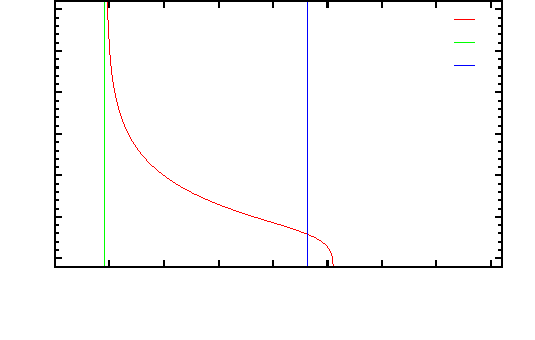
\includegraphics{c2_plot_potentials_WCA_hs}}%
    \gplfronttext
  \end{picture}%
\endgroup
} \hfill
%   \caption{ 
%   }
%  \label{fig:}
% \end{figure}

%All that remains to specify the model is a concrete attractive perturbation.

Next we model the attractive perturbation. 
To do so, we begin with a model for the full two particle interaction 
and then split it into attractive and repulsive parts, according the WCA procedure.
For small symmetric molecules the Lennard-Jones 6-12 potential has good accuracy.
It is given by
\begin{align}
  \phi_\LJ(r) = 4\epsilon\lr{\frac{\sigma^{12}}{r^{12}} - \frac{\sigma^{6}}{r^{6}}}
  \label{eqn:nuc:LJ}
\end{align}
where $r = \abs{\vr=\vr^\prime}$, $\eta$ is the characteristic bond energy 
and $\sigma$ the characteristic length.
The Kihira-potential does a better job for larger models such as perfluoropentane 
but greatly complicates the approach.
The Lennard-Jones potential is used  in this thesis.

% The Kihira-potential is an extension to approximate assymmetric molecules.
% It remains a symmetric potential, 
% but it includes a hard sphere of radius $r$ of excluded volume.
% \begin{align}
%   \phi_\K(r) = 4\epsilon\lr{\frac{\lr{\sigma-2a}^{12}}{\lr{r-2a}^{12}} - \frac{\lr{\sigma-2a}^{6}}{\lr{r-2a}^{6}}}
% \end{align}
% Oh\cite{Oh2010} recently fitted the Kihira-potential to the measured  second viral coefficient and viscosity 
% of the perlfuoroalkane series.
% The calculated potentials are plotted in \figref{Kihira_potentials}

The potentials are then separated into attractive and repulsive parts, $\phi_\attr$ and $\phi_\rep$, respectively,
\begin{align}
  \phi_\rep^\WCA(r) = \left\{
    \begin{array}{ll}
      \phi(r) +  \epsilon & \text{if $r<r_\min$}\\
      0 & \text{otherwise}
    \end{array} \right. 
\end{align}
and 
\begin{align}
  \phi_\attr^\WCA(r) = \left\{ 
    \begin{array}{ll}
      - \epsilon & \text{if $r<r_\min$}\\
      \phi(r) & \text{otherwise}
    \end{array} \right.
\end{align}
where $r_\min$ is the radius at which the potential is minimal.

It is useful at this stage to define the integrated strength of the attractive potential, 
\begin{align}
  \alpha =  - \iint d \vr_i d\vr_j \phi_\attr( \vr_i, \vr_j).
  \label{eqn:nuc:alpha}
\end{align}

Finally to reestablish contact with the hard sphere approximation 
the repulsive part of the decomposition is replaced by an infinite repulsion at a distance $d$,
That is 
\begin{align}
  \phi_\hs(r) = \left\{
    \begin{array}{ll}
      \infty & \text{if $r<d$}\\
      0 & \text{otherwise}
    \end{array} \right. .
\end{align}

%This WCA decomposition is plotted for \pfp\ in \figref{Kihira_WCA}.
%\subsubsection{Approximations}
Equation \eqnref{F_pert} is still exact for two particle potential theories.
In order to solve it we first  assume that the  hard sphere potential is a function only of the local density,
\begin{align}
  F_\hs \lrs{\rho} \approx \int d\vr f_\hs(\rho(\vr)). \label{eqn:LDA}
\end{align}
$f_\hs(\rho(\vr))$ is the potential (per unit volume) of a uniform  hard-sphere fluid\cite{Evans1992}.
It is obtained from the accurate  Carnahan-Stirling equation of state,
\begin{align}
    \fh(\rho(\vr)) =  f_\ideal + \rho \kB T\frac{4\eta - 3\eta^2}{\lr{1-\eta}^2}
  \label{eqn:nuc:CS}
\end{align}
where $\eta =  \frac{\pi \rho d^3}{6}$ is the packing function and $f_\ideal =  \rho\kB T\lr{\ln \lr{\rho \lambda^3} -1}$ is the free energy (per volume) of an ideal gas.
$\lambda$ is the de Broglie wavelength.
%
%\begin{align}
%  f_\hs(\rho) = p_\hs + \mu \rho.
%\end{align}
%$f_\hs(\rho(\vr))$ can be obtained from the accurate Carnahan-Stirling equation of state.
%It is  a known (but non-linear) function of the number density.
The approximation \eqnref{LDA} is known as the {\em local-density approximation}.

The perturbation may be approximated by assuming that the two particle densities are uncorrelated, 
\begin{align}
\rho(\vr_i, \vr_j) \approx \rho(\vr_i)\rho(\vr_j).\label{eqn:RPA}
\end{align}
This is known as the {\em random phase approximation}.
%The approximation has been found to be accurate in the absence of rapid \todo{get this sentence right} \cite.
If the medium is sufficiently large then this approximation should hold\cite{Evans1992}.
The random phase approximation may well need to be refined for very small oil droplet in water,  
where the oil-water interface cannot be ignored.

Equation \eqnref{OmegaVDefn} can therefore be written as an explicit function of $\rho$,
\begin{align}
   \Omega_V = \int d\vr f_\hs(\rho(\vr))  +   \iint d \vr_i d\vr_j \phi_\attr( \vr_i, \vr_j) \rho(\vr_i)\rho(\vr_j) -  \mu \int d\vr \rho(\vr),  \label{eqn:OmegaV}
\end{align}
where equations \eqnref{F_pert}, \eqnref{LDA} and \eqnref{RPA} have been used.
Minimising \eqnref{OmegaV} with respect to $\rho(\vr)$ gives
\begin{align}
  \frac{\delta  f_\hs(\rho(\vr)) }{\delta \rho(\vr)} \equiv \mu_\hs\lrs{\rho(\vr)} = \mu - \int d\vr^\prime \phi_\attr( \vr, \vr^\prime) \rho(\vr^\prime). \label{eqn:ChemPots}
\end{align}
$\mu_\hs\lrs{\rho(\vr)}$ is the chemical potential of the hard sphere fluid\footnote{
The chemical potential of a hard sphere fluid is given by 
\begin{align}
 \mu_\hs = \frac{d \fh}{d \rho} =  \kB T\frac{8\eta - 9 \eta^2 + 3\eta^3}{\lr{1-\eta}^3} + \kB \ln \lr{\rho \lambda^3}
\end{align}
}.

All the terms on in \eqnref{ChemPots} can be obtained for a given function density profile.
$\mu_\hs$ on the left and the second term on the right hand side have explicit representations, while
the chemical potential $\mu$ `mean field' obtained by analysing the bulk properties of the fluid.
Equation \eqnref{ChemPots} can therefore be solved by iteration.
An initial guess as the density profile is given to the right hand side.
The chemical potential $\mu_\hs$ is then inverted (numerically) to give an improved estimate of $\rho$.
%This procedure is carried out for the perfluorocarbons in \secref{}.

The density obtained by solving \eqnref{ChemPots} is the density that minimises $\Omega_V$,
and it therefore gives the best approximation the true equilibrium grand potential.
The bubble is only in thermodynamic equilibrium when it is at its critical radius.
Therefore the density $\rho$ obtained from \eqnref{ChemPots} is the density profile of the critical bubble.
%With this we may obtain an improved estimate of the surface tension and estimate a more reliable nucleation rate.

\subsubsection{Fit the model parameters}\label{sec:nuc:DFT:fit}

To use equation \eqnref{ChemPots} 
we need to define the free parameters in our model.
There are four parameters in total, of which three are independent,
\nlist{
\item $\epsilon$ - the energy scale in the Lennard-Jones 6-12 potential (equation \eqnref{nuc:LJ}),
\item $\sigma$ - the length scale in the Lennard-Jones 6-12 potential (equation \eqnref{nuc:LJ}),
\item $\alpha$ - the attractive stength of the Lennard-Jones 6-12 potential (equation \eqnref{nuc:alpha}),
\item $d$ - The length scale in the hard-sphere model (equation \eqnref{nuc:CS}).
}

Two of the parameters can be set by considering the bulk fluid.
If the density is uniform then equation \eqnref{OmegaV} becomes
\begin{align}
   \Omega_V/V =  f_\hs(\rho)  -  \tfrac{1}{2}\alpha \rho^2 -  \mu \rho= p_\hs + \mu_\hs \rho  -  \tfrac{1}{2} \alpha \rho^2 -  \mu \rho. \label{eqn:nuc:OmegaVBulk}
\end{align}
where $V$ is the volume of the system%. %and 
%\begin{align}
%  \alpha =  - \iint d \vr_i d\vr_j \phi_\attr( \vr_i, \vr_j)
%\end{align}
%is the total attractive contribution from the perturbation.
\footnote{The hard sphere pressure is given by
\begin{align}
 p_\hs = \kB T \rho \frac{1+\eta +\eta^2-\eta^3}{1-\eta^3}. \label{eqn:nuc:HSpressure}
\end{align}
}.

Equation \Eqnref{nuc:OmegaVBulk}  can be minimised with the help of the Maxwell relation
\begin{align}
  \frac{\d p_\hs}{\d \rho} = \rho \frac{\d \mu_\hs}{\d \rho} 
\end{align}
to obtain
\begin{align}
  \mu = \mu_\hs - \alpha \rho. \label{eqn:nuc:muBulk}
\end{align}
Substituting \eqnref{nuc:muBulk} into \eqnref{nuc:OmegaVBulk} gives
\begin{align}
   \Omega_V/V = -p_\hs(\rho) + \half \alpha \rho^2 = -p.
   \label{eqn:nuc:OmegaVBulkP}
\end{align}
Equation \eqnref{nuc:OmegaVBulkP} depends only on $d$ and $\alpha$.

Below the critical temperature there will be 
two phases in  bulk coexistence.
The number densities of these two phases are $\rho_v$ and $\rho_L$,
where the ``$v$'' denotes the vapour and the ``$L$'' denotes the liquid.
%as in \secref{nuc:CNT}.
At equilibrium the chemical potential and the pressures for both phases are equal
\sub{
\label{eqn:BulkCoex}
\begin{align}
  \mu_v = \mu_\hs(\rho_v) - \alpha \rho_v &= \mu_\hs(\rho_L) - \alpha \rho_L = \mu_L,\\
  p_v = p_\hs(\rho_v) - \half \alpha \rho_v^2 &= p_\hs(\rho_L) - \half \alpha \rho_L^2 = p_L.
\end{align}
}
The solutions of equations \eqnref{BulkCoex} define the coexistance curve for the fluid,
and they may be used to obtain the two parameters $d$ and $\alpha$.

The final parameter, $\sigma$ (or equivalently $\epsilon$) is obtained from the measured surface tension of the fluid.
The value of $\Omega$ is obtained by iterating \eqnref{ChemPots}.  
The surface tension is then calculated by noting that
\begin{align}
  \Omega_V = \Omega_{V_l} + \Omega_{V_g} + \gamma A,
\end{align}
where $\Omega_{V_l}$ and $\Omega_{V_g}$ are the potentials of the bulk liquid and gas evaluated at the Gibbs surface,
$\gamma$ is the surface tension and $A$ is the area of the surface.
The value of $\sigma$ is chosen so that the calculated value of $\gamma$ matches its experimental value.


The code to solve these equations was written by the author of this thesis and is freely available on github\cite{NucleationCode}.

\subsection{Results of the density functional approach}\label{sec:nuc:DFT:results}


\begin{figure}
 \centering
  \subfloat[Coexistence for water]{% GNUPLOT: LaTeX picture with Postscript
\begingroup
  \makeatletter
  \providecommand\color[2][]{%
    \GenericError{(gnuplot) \space\space\space\@spaces}{%
      Package color not loaded in conjunction with
      terminal option `colourtext'%
    }{See the gnuplot documentation for explanation.%
    }{Either use 'blacktext' in gnuplot or load the package
      color.sty in LaTeX.}%
    \renewcommand\color[2][]{}%
  }%
  \providecommand\includegraphics[2][]{%
    \GenericError{(gnuplot) \space\space\space\@spaces}{%
      Package graphicx or graphics not loaded%
    }{See the gnuplot documentation for explanation.%
    }{The gnuplot epslatex terminal needs graphicx.sty or graphics.sty.}%
    \renewcommand\includegraphics[2][]{}%
  }%
  \providecommand\rotatebox[2]{#2}%
  \@ifundefined{ifGPcolor}{%
    \newif\ifGPcolor
    \GPcolorfalse
  }{}%
  \@ifundefined{ifGPblacktext}{%
    \newif\ifGPblacktext
    \GPblacktexttrue
  }{}%
  % define a \g@addto@macro without @ in the name:
  \let\gplgaddtomacro\g@addto@macro
  % define empty templates for all commands taking text:
  \gdef\gplbacktext{}%
  \gdef\gplfronttext{}%
  \makeatother
  \ifGPblacktext
    % no textcolor at all
    \def\colorrgb#1{}%
    \def\colorgray#1{}%
  \else
    % gray or color?
    \ifGPcolor
      \def\colorrgb#1{\color[rgb]{#1}}%
      \def\colorgray#1{\color[gray]{#1}}%
      \expandafter\def\csname LTw\endcsname{\color{white}}%
      \expandafter\def\csname LTb\endcsname{\color{black}}%
      \expandafter\def\csname LTa\endcsname{\color{black}}%
      \expandafter\def\csname LT0\endcsname{\color[rgb]{1,0,0}}%
      \expandafter\def\csname LT1\endcsname{\color[rgb]{0,1,0}}%
      \expandafter\def\csname LT2\endcsname{\color[rgb]{0,0,1}}%
      \expandafter\def\csname LT3\endcsname{\color[rgb]{1,0,1}}%
      \expandafter\def\csname LT4\endcsname{\color[rgb]{0,1,1}}%
      \expandafter\def\csname LT5\endcsname{\color[rgb]{1,1,0}}%
      \expandafter\def\csname LT6\endcsname{\color[rgb]{0,0,0}}%
      \expandafter\def\csname LT7\endcsname{\color[rgb]{1,0.3,0}}%
      \expandafter\def\csname LT8\endcsname{\color[rgb]{0.5,0.5,0.5}}%
    \else
      % gray
      \def\colorrgb#1{\color{black}}%
      \def\colorgray#1{\color[gray]{#1}}%
      \expandafter\def\csname LTw\endcsname{\color{white}}%
      \expandafter\def\csname LTb\endcsname{\color{black}}%
      \expandafter\def\csname LTa\endcsname{\color{black}}%
      \expandafter\def\csname LT0\endcsname{\color{black}}%
      \expandafter\def\csname LT1\endcsname{\color{black}}%
      \expandafter\def\csname LT2\endcsname{\color{black}}%
      \expandafter\def\csname LT3\endcsname{\color{black}}%
      \expandafter\def\csname LT4\endcsname{\color{black}}%
      \expandafter\def\csname LT5\endcsname{\color{black}}%
      \expandafter\def\csname LT6\endcsname{\color{black}}%
      \expandafter\def\csname LT7\endcsname{\color{black}}%
      \expandafter\def\csname LT8\endcsname{\color{black}}%
    \fi
  \fi
  \setlength{\unitlength}{0.0500bp}%
  \begin{picture}(7200.00,5040.00)%
    \gplgaddtomacro\gplbacktext{%
      \csname LTb\endcsname%
      \put(946,704){\makebox(0,0)[r]{\strut{} 250}}%
      \put(946,1213){\makebox(0,0)[r]{\strut{} 300}}%
      \put(946,1722){\makebox(0,0)[r]{\strut{} 350}}%
      \put(946,2231){\makebox(0,0)[r]{\strut{} 400}}%
      \put(946,2740){\makebox(0,0)[r]{\strut{} 450}}%
      \put(946,3248){\makebox(0,0)[r]{\strut{} 500}}%
      \put(946,3757){\makebox(0,0)[r]{\strut{} 550}}%
      \put(946,4266){\makebox(0,0)[r]{\strut{} 600}}%
      \put(946,4775){\makebox(0,0)[r]{\strut{} 650}}%
      \put(1078,484){\makebox(0,0){\strut{} 0}}%
      \put(1651,484){\makebox(0,0){\strut{} 100}}%
      \put(2223,484){\makebox(0,0){\strut{} 200}}%
      \put(2796,484){\makebox(0,0){\strut{} 300}}%
      \put(3368,484){\makebox(0,0){\strut{} 400}}%
      \put(3941,484){\makebox(0,0){\strut{} 500}}%
      \put(4513,484){\makebox(0,0){\strut{} 600}}%
      \put(5086,484){\makebox(0,0){\strut{} 700}}%
      \put(5658,484){\makebox(0,0){\strut{} 800}}%
      \put(6231,484){\makebox(0,0){\strut{} 900}}%
      \put(6803,484){\makebox(0,0){\strut{} 1000}}%
      \put(176,2739){\rotatebox{-270}{\makebox(0,0){\strut{}temperature ($K$)}}}%
      \put(3940,154){\makebox(0,0){\strut{}density ($kg/m^3$)}}%
    }%
    \gplgaddtomacro\gplfronttext{%
      \csname LTb\endcsname%
      \put(5816,4602){\makebox(0,0)[r]{\strut{}coexistence}}%
      \csname LTb\endcsname%
      \put(5816,4382){\makebox(0,0)[r]{\strut{}measured}}%
      \csname LTb\endcsname%
      \put(5816,4162){\makebox(0,0)[r]{\strut{}spinodal}}%
    }%
    \gplbacktext
    \put(0,0){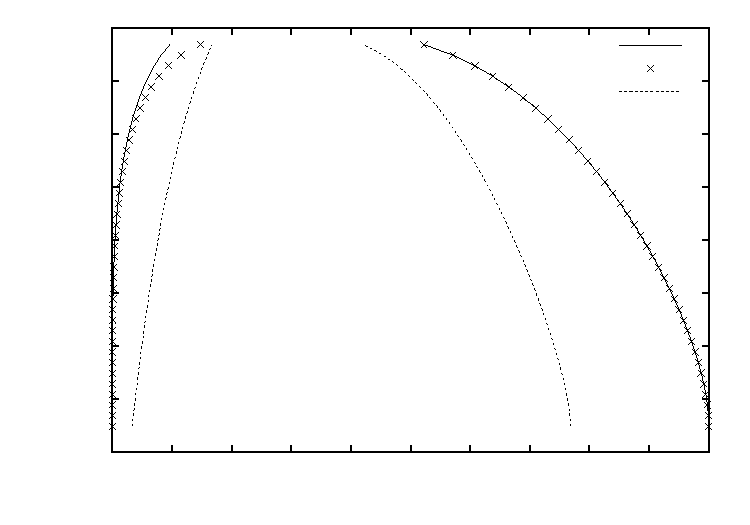
\includegraphics{chNucCoexWater}}%
    \gplfronttext
  \end{picture}%
\endgroup
}\\
  \subfloat[Coexistence for \pfp]{% GNUPLOT: LaTeX picture with Postscript
\begingroup
  \makeatletter
  \providecommand\color[2][]{%
    \GenericError{(gnuplot) \space\space\space\@spaces}{%
      Package color not loaded in conjunction with
      terminal option `colourtext'%
    }{See the gnuplot documentation for explanation.%
    }{Either use 'blacktext' in gnuplot or load the package
      color.sty in LaTeX.}%
    \renewcommand\color[2][]{}%
  }%
  \providecommand\includegraphics[2][]{%
    \GenericError{(gnuplot) \space\space\space\@spaces}{%
      Package graphicx or graphics not loaded%
    }{See the gnuplot documentation for explanation.%
    }{The gnuplot epslatex terminal needs graphicx.sty or graphics.sty.}%
    \renewcommand\includegraphics[2][]{}%
  }%
  \providecommand\rotatebox[2]{#2}%
  \@ifundefined{ifGPcolor}{%
    \newif\ifGPcolor
    \GPcolorfalse
  }{}%
  \@ifundefined{ifGPblacktext}{%
    \newif\ifGPblacktext
    \GPblacktexttrue
  }{}%
  % define a \g@addto@macro without @ in the name:
  \let\gplgaddtomacro\g@addto@macro
  % define empty templates for all commands taking text:
  \gdef\gplbacktext{}%
  \gdef\gplfronttext{}%
  \makeatother
  \ifGPblacktext
    % no textcolor at all
    \def\colorrgb#1{}%
    \def\colorgray#1{}%
  \else
    % gray or color?
    \ifGPcolor
      \def\colorrgb#1{\color[rgb]{#1}}%
      \def\colorgray#1{\color[gray]{#1}}%
      \expandafter\def\csname LTw\endcsname{\color{white}}%
      \expandafter\def\csname LTb\endcsname{\color{black}}%
      \expandafter\def\csname LTa\endcsname{\color{black}}%
      \expandafter\def\csname LT0\endcsname{\color[rgb]{1,0,0}}%
      \expandafter\def\csname LT1\endcsname{\color[rgb]{0,1,0}}%
      \expandafter\def\csname LT2\endcsname{\color[rgb]{0,0,1}}%
      \expandafter\def\csname LT3\endcsname{\color[rgb]{1,0,1}}%
      \expandafter\def\csname LT4\endcsname{\color[rgb]{0,1,1}}%
      \expandafter\def\csname LT5\endcsname{\color[rgb]{1,1,0}}%
      \expandafter\def\csname LT6\endcsname{\color[rgb]{0,0,0}}%
      \expandafter\def\csname LT7\endcsname{\color[rgb]{1,0.3,0}}%
      \expandafter\def\csname LT8\endcsname{\color[rgb]{0.5,0.5,0.5}}%
    \else
      % gray
      \def\colorrgb#1{\color{black}}%
      \def\colorgray#1{\color[gray]{#1}}%
      \expandafter\def\csname LTw\endcsname{\color{white}}%
      \expandafter\def\csname LTb\endcsname{\color{black}}%
      \expandafter\def\csname LTa\endcsname{\color{black}}%
      \expandafter\def\csname LT0\endcsname{\color{black}}%
      \expandafter\def\csname LT1\endcsname{\color{black}}%
      \expandafter\def\csname LT2\endcsname{\color{black}}%
      \expandafter\def\csname LT3\endcsname{\color{black}}%
      \expandafter\def\csname LT4\endcsname{\color{black}}%
      \expandafter\def\csname LT5\endcsname{\color{black}}%
      \expandafter\def\csname LT6\endcsname{\color{black}}%
      \expandafter\def\csname LT7\endcsname{\color{black}}%
      \expandafter\def\csname LT8\endcsname{\color{black}}%
    \fi
  \fi
  \setlength{\unitlength}{0.0500bp}%
  \begin{picture}(7200.00,5040.00)%
    \gplgaddtomacro\gplbacktext{%
      \csname LTb\endcsname%
      \put(946,704){\makebox(0,0)[r]{\strut{} 200}}%
      \put(946,1518){\makebox(0,0)[r]{\strut{} 250}}%
      \put(946,2332){\makebox(0,0)[r]{\strut{} 300}}%
      \put(946,3147){\makebox(0,0)[r]{\strut{} 350}}%
      \put(946,3961){\makebox(0,0)[r]{\strut{} 400}}%
      \put(946,4775){\makebox(0,0)[r]{\strut{} 450}}%
      \put(1078,484){\makebox(0,0){\strut{} 0}}%
      \put(1651,484){\makebox(0,0){\strut{} 200}}%
      \put(2223,484){\makebox(0,0){\strut{} 400}}%
      \put(2796,484){\makebox(0,0){\strut{} 600}}%
      \put(3368,484){\makebox(0,0){\strut{} 800}}%
      \put(3941,484){\makebox(0,0){\strut{} 1000}}%
      \put(4513,484){\makebox(0,0){\strut{} 1200}}%
      \put(5086,484){\makebox(0,0){\strut{} 1400}}%
      \put(5658,484){\makebox(0,0){\strut{} 1600}}%
      \put(6231,484){\makebox(0,0){\strut{} 1800}}%
      \put(6803,484){\makebox(0,0){\strut{} 2000}}%
      \put(176,2739){\rotatebox{-270}{\makebox(0,0){\strut{}temperature ($K$)}}}%
      \put(3940,154){\makebox(0,0){\strut{}density ($kg/m^3$)}}%
    }%
    \gplgaddtomacro\gplfronttext{%
      \csname LTb\endcsname%
      \put(5816,4602){\makebox(0,0)[r]{\strut{}coexistence}}%
      \csname LTb\endcsname%
      \put(5816,4382){\makebox(0,0)[r]{\strut{}measured}}%
      \csname LTb\endcsname%
      \put(5816,4162){\makebox(0,0)[r]{\strut{}spinodal}}%
    }%
    \gplbacktext
    \put(0,0){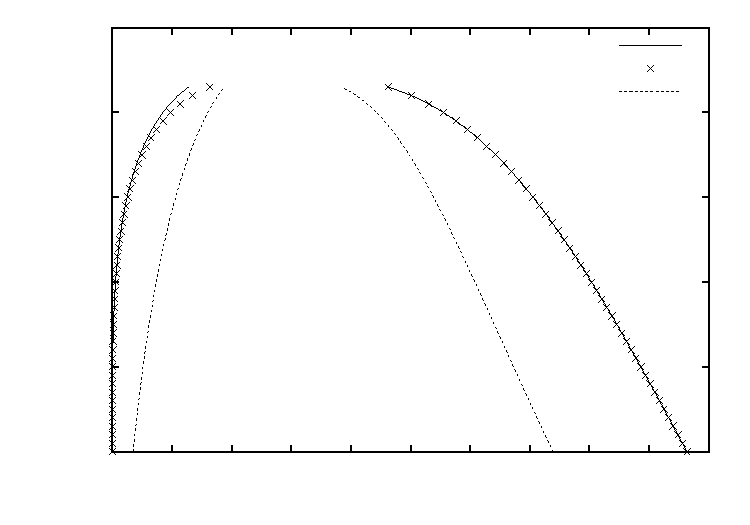
\includegraphics{chNucCoexPfp}}%
    \gplfronttext
  \end{picture}%
\endgroup
}
  \caption{Coexistence and spinodal curve for water and \pfp.
    The plot was used to obtain the temperature dependence of the parameters $d$ and $\epsilon$ 
    in the hard-sphere model with Lennard-Jones interactions.
  }
 \label{fig:nuc:coex}
\end{figure}

\begin{figure}
 \centering
  \subfloat[The parameter $d$ for water]{% GNUPLOT: LaTeX picture with Postscript
\begingroup
  \makeatletter
  \providecommand\color[2][]{%
    \GenericError{(gnuplot) \space\space\space\@spaces}{%
      Package color not loaded in conjunction with
      terminal option `colourtext'%
    }{See the gnuplot documentation for explanation.%
    }{Either use 'blacktext' in gnuplot or load the package
      color.sty in LaTeX.}%
    \renewcommand\color[2][]{}%
  }%
  \providecommand\includegraphics[2][]{%
    \GenericError{(gnuplot) \space\space\space\@spaces}{%
      Package graphicx or graphics not loaded%
    }{See the gnuplot documentation for explanation.%
    }{The gnuplot epslatex terminal needs graphicx.sty or graphics.sty.}%
    \renewcommand\includegraphics[2][]{}%
  }%
  \providecommand\rotatebox[2]{#2}%
  \@ifundefined{ifGPcolor}{%
    \newif\ifGPcolor
    \GPcolorfalse
  }{}%
  \@ifundefined{ifGPblacktext}{%
    \newif\ifGPblacktext
    \GPblacktexttrue
  }{}%
  % define a \g@addto@macro without @ in the name:
  \let\gplgaddtomacro\g@addto@macro
  % define empty templates for all commands taking text:
  \gdef\gplbacktext{}%
  \gdef\gplfronttext{}%
  \makeatother
  \ifGPblacktext
    % no textcolor at all
    \def\colorrgb#1{}%
    \def\colorgray#1{}%
  \else
    % gray or color?
    \ifGPcolor
      \def\colorrgb#1{\color[rgb]{#1}}%
      \def\colorgray#1{\color[gray]{#1}}%
      \expandafter\def\csname LTw\endcsname{\color{white}}%
      \expandafter\def\csname LTb\endcsname{\color{black}}%
      \expandafter\def\csname LTa\endcsname{\color{black}}%
      \expandafter\def\csname LT0\endcsname{\color[rgb]{1,0,0}}%
      \expandafter\def\csname LT1\endcsname{\color[rgb]{0,1,0}}%
      \expandafter\def\csname LT2\endcsname{\color[rgb]{0,0,1}}%
      \expandafter\def\csname LT3\endcsname{\color[rgb]{1,0,1}}%
      \expandafter\def\csname LT4\endcsname{\color[rgb]{0,1,1}}%
      \expandafter\def\csname LT5\endcsname{\color[rgb]{1,1,0}}%
      \expandafter\def\csname LT6\endcsname{\color[rgb]{0,0,0}}%
      \expandafter\def\csname LT7\endcsname{\color[rgb]{1,0.3,0}}%
      \expandafter\def\csname LT8\endcsname{\color[rgb]{0.5,0.5,0.5}}%
    \else
      % gray
      \def\colorrgb#1{\color{black}}%
      \def\colorgray#1{\color[gray]{#1}}%
      \expandafter\def\csname LTw\endcsname{\color{white}}%
      \expandafter\def\csname LTb\endcsname{\color{black}}%
      \expandafter\def\csname LTa\endcsname{\color{black}}%
      \expandafter\def\csname LT0\endcsname{\color{black}}%
      \expandafter\def\csname LT1\endcsname{\color{black}}%
      \expandafter\def\csname LT2\endcsname{\color{black}}%
      \expandafter\def\csname LT3\endcsname{\color{black}}%
      \expandafter\def\csname LT4\endcsname{\color{black}}%
      \expandafter\def\csname LT5\endcsname{\color{black}}%
      \expandafter\def\csname LT6\endcsname{\color{black}}%
      \expandafter\def\csname LT7\endcsname{\color{black}}%
      \expandafter\def\csname LT8\endcsname{\color{black}}%
    \fi
  \fi
  \setlength{\unitlength}{0.0500bp}%
  \begin{picture}(4320.00,3024.00)%
    \gplgaddtomacro\gplbacktext{%
      \csname LTb\endcsname%
      \put(990,704){\makebox(0,0)[r]{\strut{} 0.294}}%
      \put(990,910){\makebox(0,0)[r]{\strut{} 0.296}}%
      \put(990,1115){\makebox(0,0)[r]{\strut{} 0.298}}%
      \put(990,1321){\makebox(0,0)[r]{\strut{} 0.3}}%
      \put(990,1526){\makebox(0,0)[r]{\strut{} 0.302}}%
      \put(990,1732){\makebox(0,0)[r]{\strut{} 0.304}}%
      \put(990,1937){\makebox(0,0)[r]{\strut{} 0.306}}%
      \put(990,2143){\makebox(0,0)[r]{\strut{} 0.308}}%
      \put(990,2348){\makebox(0,0)[r]{\strut{} 0.31}}%
      \put(990,2554){\makebox(0,0)[r]{\strut{} 0.312}}%
      \put(990,2759){\makebox(0,0)[r]{\strut{} 0.314}}%
      \put(1122,484){\makebox(0,0){\strut{} 250}}%
      \put(1522,484){\makebox(0,0){\strut{} 300}}%
      \put(1921,484){\makebox(0,0){\strut{} 350}}%
      \put(2321,484){\makebox(0,0){\strut{} 400}}%
      \put(2721,484){\makebox(0,0){\strut{} 450}}%
      \put(3120,484){\makebox(0,0){\strut{} 500}}%
      \put(3520,484){\makebox(0,0){\strut{} 550}}%
      \put(3919,484){\makebox(0,0){\strut{} 600}}%
      \put(4319,484){\makebox(0,0){\strut{} 650}}%
      \put(352,1731){\rotatebox{-270}{\makebox(0,0){\strut{}$d$ ($nm$)}}}%
      \put(2720,154){\makebox(0,0){\strut{}temperature ($K$)}}%
    }%
    \gplgaddtomacro\gplfronttext{%
    }%
    \gplbacktext
    \put(0,0){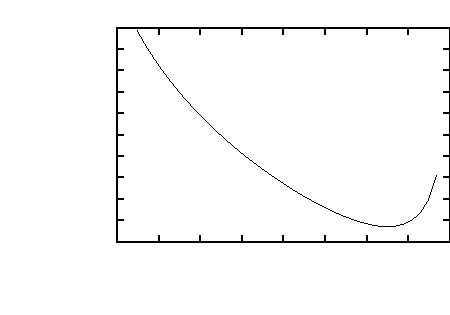
\includegraphics{chNucParamsDWater}}%
    \gplfronttext
  \end{picture}%
\endgroup
}
  \subfloat[The parameter $\epsilon$ for  water]{% GNUPLOT: LaTeX picture with Postscript
\begingroup
  \makeatletter
  \providecommand\color[2][]{%
    \GenericError{(gnuplot) \space\space\space\@spaces}{%
      Package color not loaded in conjunction with
      terminal option `colourtext'%
    }{See the gnuplot documentation for explanation.%
    }{Either use 'blacktext' in gnuplot or load the package
      color.sty in LaTeX.}%
    \renewcommand\color[2][]{}%
  }%
  \providecommand\includegraphics[2][]{%
    \GenericError{(gnuplot) \space\space\space\@spaces}{%
      Package graphicx or graphics not loaded%
    }{See the gnuplot documentation for explanation.%
    }{The gnuplot epslatex terminal needs graphicx.sty or graphics.sty.}%
    \renewcommand\includegraphics[2][]{}%
  }%
  \providecommand\rotatebox[2]{#2}%
  \@ifundefined{ifGPcolor}{%
    \newif\ifGPcolor
    \GPcolorfalse
  }{}%
  \@ifundefined{ifGPblacktext}{%
    \newif\ifGPblacktext
    \GPblacktexttrue
  }{}%
  % define a \g@addto@macro without @ in the name:
  \let\gplgaddtomacro\g@addto@macro
  % define empty templates for all commands taking text:
  \gdef\gplbacktext{}%
  \gdef\gplfronttext{}%
  \makeatother
  \ifGPblacktext
    % no textcolor at all
    \def\colorrgb#1{}%
    \def\colorgray#1{}%
  \else
    % gray or color?
    \ifGPcolor
      \def\colorrgb#1{\color[rgb]{#1}}%
      \def\colorgray#1{\color[gray]{#1}}%
      \expandafter\def\csname LTw\endcsname{\color{white}}%
      \expandafter\def\csname LTb\endcsname{\color{black}}%
      \expandafter\def\csname LTa\endcsname{\color{black}}%
      \expandafter\def\csname LT0\endcsname{\color[rgb]{1,0,0}}%
      \expandafter\def\csname LT1\endcsname{\color[rgb]{0,1,0}}%
      \expandafter\def\csname LT2\endcsname{\color[rgb]{0,0,1}}%
      \expandafter\def\csname LT3\endcsname{\color[rgb]{1,0,1}}%
      \expandafter\def\csname LT4\endcsname{\color[rgb]{0,1,1}}%
      \expandafter\def\csname LT5\endcsname{\color[rgb]{1,1,0}}%
      \expandafter\def\csname LT6\endcsname{\color[rgb]{0,0,0}}%
      \expandafter\def\csname LT7\endcsname{\color[rgb]{1,0.3,0}}%
      \expandafter\def\csname LT8\endcsname{\color[rgb]{0.5,0.5,0.5}}%
    \else
      % gray
      \def\colorrgb#1{\color{black}}%
      \def\colorgray#1{\color[gray]{#1}}%
      \expandafter\def\csname LTw\endcsname{\color{white}}%
      \expandafter\def\csname LTb\endcsname{\color{black}}%
      \expandafter\def\csname LTa\endcsname{\color{black}}%
      \expandafter\def\csname LT0\endcsname{\color{black}}%
      \expandafter\def\csname LT1\endcsname{\color{black}}%
      \expandafter\def\csname LT2\endcsname{\color{black}}%
      \expandafter\def\csname LT3\endcsname{\color{black}}%
      \expandafter\def\csname LT4\endcsname{\color{black}}%
      \expandafter\def\csname LT5\endcsname{\color{black}}%
      \expandafter\def\csname LT6\endcsname{\color{black}}%
      \expandafter\def\csname LT7\endcsname{\color{black}}%
      \expandafter\def\csname LT8\endcsname{\color{black}}%
    \fi
  \fi
  \setlength{\unitlength}{0.0500bp}%
  \begin{picture}(4320.00,3024.00)%
    \gplgaddtomacro\gplbacktext{%
      \csname LTb\endcsname%
      \put(726,704){\makebox(0,0)[r]{\strut{}-105}}%
      \put(726,998){\makebox(0,0)[r]{\strut{}-100}}%
      \put(726,1291){\makebox(0,0)[r]{\strut{}-95}}%
      \put(726,1585){\makebox(0,0)[r]{\strut{}-90}}%
      \put(726,1878){\makebox(0,0)[r]{\strut{}-85}}%
      \put(726,2172){\makebox(0,0)[r]{\strut{}-80}}%
      \put(726,2465){\makebox(0,0)[r]{\strut{}-75}}%
      \put(726,2759){\makebox(0,0)[r]{\strut{}-70}}%
      \put(858,484){\makebox(0,0){\strut{} 250}}%
      \put(1241,484){\makebox(0,0){\strut{} 300}}%
      \put(1624,484){\makebox(0,0){\strut{} 350}}%
      \put(2007,484){\makebox(0,0){\strut{} 400}}%
      \put(2391,484){\makebox(0,0){\strut{} 450}}%
      \put(2774,484){\makebox(0,0){\strut{} 500}}%
      \put(3157,484){\makebox(0,0){\strut{} 550}}%
      \put(3540,484){\makebox(0,0){\strut{} 600}}%
      \put(3923,484){\makebox(0,0){\strut{} 650}}%
      \put(352,1731){\rotatebox{-270}{\makebox(0,0){\strut{}$\epsilon$ ($zJ$)}}}%
      \put(2390,154){\makebox(0,0){\strut{}temperature ($K$)}}%
    }%
    \gplgaddtomacro\gplfronttext{%
    }%
    \gplbacktext
    \put(0,0){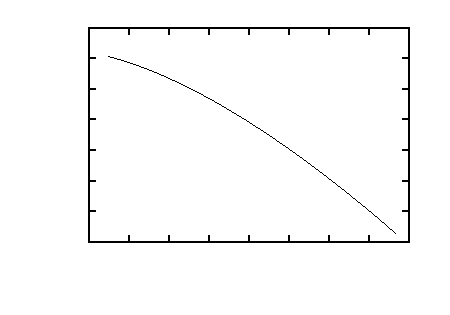
\includegraphics{chNucParamsEWater}}%
    \gplfronttext
  \end{picture}%
\endgroup
}\\
  \subfloat[The parameter $d$ for \pfp]{% GNUPLOT: LaTeX picture with Postscript
\begingroup
  \makeatletter
  \providecommand\color[2][]{%
    \GenericError{(gnuplot) \space\space\space\@spaces}{%
      Package color not loaded in conjunction with
      terminal option `colourtext'%
    }{See the gnuplot documentation for explanation.%
    }{Either use 'blacktext' in gnuplot or load the package
      color.sty in LaTeX.}%
    \renewcommand\color[2][]{}%
  }%
  \providecommand\includegraphics[2][]{%
    \GenericError{(gnuplot) \space\space\space\@spaces}{%
      Package graphicx or graphics not loaded%
    }{See the gnuplot documentation for explanation.%
    }{The gnuplot epslatex terminal needs graphicx.sty or graphics.sty.}%
    \renewcommand\includegraphics[2][]{}%
  }%
  \providecommand\rotatebox[2]{#2}%
  \@ifundefined{ifGPcolor}{%
    \newif\ifGPcolor
    \GPcolorfalse
  }{}%
  \@ifundefined{ifGPblacktext}{%
    \newif\ifGPblacktext
    \GPblacktexttrue
  }{}%
  % define a \g@addto@macro without @ in the name:
  \let\gplgaddtomacro\g@addto@macro
  % define empty templates for all commands taking text:
  \gdef\gplbacktext{}%
  \gdef\gplfronttext{}%
  \makeatother
  \ifGPblacktext
    % no textcolor at all
    \def\colorrgb#1{}%
    \def\colorgray#1{}%
  \else
    % gray or color?
    \ifGPcolor
      \def\colorrgb#1{\color[rgb]{#1}}%
      \def\colorgray#1{\color[gray]{#1}}%
      \expandafter\def\csname LTw\endcsname{\color{white}}%
      \expandafter\def\csname LTb\endcsname{\color{black}}%
      \expandafter\def\csname LTa\endcsname{\color{black}}%
      \expandafter\def\csname LT0\endcsname{\color[rgb]{1,0,0}}%
      \expandafter\def\csname LT1\endcsname{\color[rgb]{0,1,0}}%
      \expandafter\def\csname LT2\endcsname{\color[rgb]{0,0,1}}%
      \expandafter\def\csname LT3\endcsname{\color[rgb]{1,0,1}}%
      \expandafter\def\csname LT4\endcsname{\color[rgb]{0,1,1}}%
      \expandafter\def\csname LT5\endcsname{\color[rgb]{1,1,0}}%
      \expandafter\def\csname LT6\endcsname{\color[rgb]{0,0,0}}%
      \expandafter\def\csname LT7\endcsname{\color[rgb]{1,0.3,0}}%
      \expandafter\def\csname LT8\endcsname{\color[rgb]{0.5,0.5,0.5}}%
    \else
      % gray
      \def\colorrgb#1{\color{black}}%
      \def\colorgray#1{\color[gray]{#1}}%
      \expandafter\def\csname LTw\endcsname{\color{white}}%
      \expandafter\def\csname LTb\endcsname{\color{black}}%
      \expandafter\def\csname LTa\endcsname{\color{black}}%
      \expandafter\def\csname LT0\endcsname{\color{black}}%
      \expandafter\def\csname LT1\endcsname{\color{black}}%
      \expandafter\def\csname LT2\endcsname{\color{black}}%
      \expandafter\def\csname LT3\endcsname{\color{black}}%
      \expandafter\def\csname LT4\endcsname{\color{black}}%
      \expandafter\def\csname LT5\endcsname{\color{black}}%
      \expandafter\def\csname LT6\endcsname{\color{black}}%
      \expandafter\def\csname LT7\endcsname{\color{black}}%
      \expandafter\def\csname LT8\endcsname{\color{black}}%
    \fi
  \fi
  \setlength{\unitlength}{0.0500bp}%
  \begin{picture}(4320.00,3024.00)%
    \gplgaddtomacro\gplbacktext{%
      \csname LTb\endcsname%
      \put(990,704){\makebox(0,0)[r]{\strut{} 0.595}}%
      \put(990,961){\makebox(0,0)[r]{\strut{} 0.6}}%
      \put(990,1218){\makebox(0,0)[r]{\strut{} 0.605}}%
      \put(990,1475){\makebox(0,0)[r]{\strut{} 0.61}}%
      \put(990,1732){\makebox(0,0)[r]{\strut{} 0.615}}%
      \put(990,1988){\makebox(0,0)[r]{\strut{} 0.62}}%
      \put(990,2245){\makebox(0,0)[r]{\strut{} 0.625}}%
      \put(990,2502){\makebox(0,0)[r]{\strut{} 0.63}}%
      \put(990,2759){\makebox(0,0)[r]{\strut{} 0.635}}%
      \put(1122,484){\makebox(0,0){\strut{} 200}}%
      \put(1761,484){\makebox(0,0){\strut{} 250}}%
      \put(2401,484){\makebox(0,0){\strut{} 300}}%
      \put(3040,484){\makebox(0,0){\strut{} 350}}%
      \put(3680,484){\makebox(0,0){\strut{} 400}}%
      \put(4319,484){\makebox(0,0){\strut{} 450}}%
      \put(352,1731){\rotatebox{-270}{\makebox(0,0){\strut{}$d$ ($nm$)}}}%
      \put(2720,154){\makebox(0,0){\strut{}temperature ($K$)}}%
    }%
    \gplgaddtomacro\gplfronttext{%
    }%
    \gplbacktext
    \put(0,0){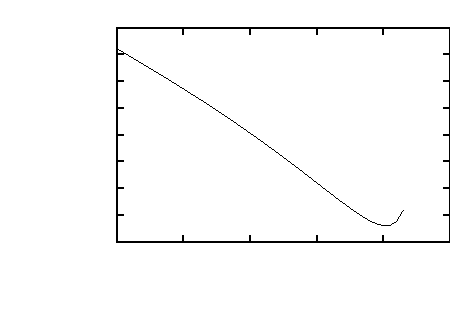
\includegraphics{chNucParamsDPfp}}%
    \gplfronttext
  \end{picture}%
\endgroup
}
  \subfloat[The parameter $\epsilon$ for \pfp]{% GNUPLOT: LaTeX picture with Postscript
\begingroup
  \makeatletter
  \providecommand\color[2][]{%
    \GenericError{(gnuplot) \space\space\space\@spaces}{%
      Package color not loaded in conjunction with
      terminal option `colourtext'%
    }{See the gnuplot documentation for explanation.%
    }{Either use 'blacktext' in gnuplot or load the package
      color.sty in LaTeX.}%
    \renewcommand\color[2][]{}%
  }%
  \providecommand\includegraphics[2][]{%
    \GenericError{(gnuplot) \space\space\space\@spaces}{%
      Package graphicx or graphics not loaded%
    }{See the gnuplot documentation for explanation.%
    }{The gnuplot epslatex terminal needs graphicx.sty or graphics.sty.}%
    \renewcommand\includegraphics[2][]{}%
  }%
  \providecommand\rotatebox[2]{#2}%
  \@ifundefined{ifGPcolor}{%
    \newif\ifGPcolor
    \GPcolorfalse
  }{}%
  \@ifundefined{ifGPblacktext}{%
    \newif\ifGPblacktext
    \GPblacktexttrue
  }{}%
  % define a \g@addto@macro without @ in the name:
  \let\gplgaddtomacro\g@addto@macro
  % define empty templates for all commands taking text:
  \gdef\gplbacktext{}%
  \gdef\gplfronttext{}%
  \makeatother
  \ifGPblacktext
    % no textcolor at all
    \def\colorrgb#1{}%
    \def\colorgray#1{}%
  \else
    % gray or color?
    \ifGPcolor
      \def\colorrgb#1{\color[rgb]{#1}}%
      \def\colorgray#1{\color[gray]{#1}}%
      \expandafter\def\csname LTw\endcsname{\color{white}}%
      \expandafter\def\csname LTb\endcsname{\color{black}}%
      \expandafter\def\csname LTa\endcsname{\color{black}}%
      \expandafter\def\csname LT0\endcsname{\color[rgb]{1,0,0}}%
      \expandafter\def\csname LT1\endcsname{\color[rgb]{0,1,0}}%
      \expandafter\def\csname LT2\endcsname{\color[rgb]{0,0,1}}%
      \expandafter\def\csname LT3\endcsname{\color[rgb]{1,0,1}}%
      \expandafter\def\csname LT4\endcsname{\color[rgb]{0,1,1}}%
      \expandafter\def\csname LT5\endcsname{\color[rgb]{1,1,0}}%
      \expandafter\def\csname LT6\endcsname{\color[rgb]{0,0,0}}%
      \expandafter\def\csname LT7\endcsname{\color[rgb]{1,0.3,0}}%
      \expandafter\def\csname LT8\endcsname{\color[rgb]{0.5,0.5,0.5}}%
    \else
      % gray
      \def\colorrgb#1{\color{black}}%
      \def\colorgray#1{\color[gray]{#1}}%
      \expandafter\def\csname LTw\endcsname{\color{white}}%
      \expandafter\def\csname LTb\endcsname{\color{black}}%
      \expandafter\def\csname LTa\endcsname{\color{black}}%
      \expandafter\def\csname LT0\endcsname{\color{black}}%
      \expandafter\def\csname LT1\endcsname{\color{black}}%
      \expandafter\def\csname LT2\endcsname{\color{black}}%
      \expandafter\def\csname LT3\endcsname{\color{black}}%
      \expandafter\def\csname LT4\endcsname{\color{black}}%
      \expandafter\def\csname LT5\endcsname{\color{black}}%
      \expandafter\def\csname LT6\endcsname{\color{black}}%
      \expandafter\def\csname LT7\endcsname{\color{black}}%
      \expandafter\def\csname LT8\endcsname{\color{black}}%
    \fi
  \fi
  \setlength{\unitlength}{0.0500bp}%
  \begin{picture}(4320.00,3024.00)%
    \gplgaddtomacro\gplbacktext{%
      \csname LTb\endcsname%
      \put(726,704){\makebox(0,0)[r]{\strut{}-100}}%
      \put(726,998){\makebox(0,0)[r]{\strut{}-95}}%
      \put(726,1291){\makebox(0,0)[r]{\strut{}-90}}%
      \put(726,1585){\makebox(0,0)[r]{\strut{}-85}}%
      \put(726,1878){\makebox(0,0)[r]{\strut{}-80}}%
      \put(726,2172){\makebox(0,0)[r]{\strut{}-75}}%
      \put(726,2465){\makebox(0,0)[r]{\strut{}-70}}%
      \put(726,2759){\makebox(0,0)[r]{\strut{}-65}}%
      \put(858,484){\makebox(0,0){\strut{} 200}}%
      \put(1471,484){\makebox(0,0){\strut{} 250}}%
      \put(2084,484){\makebox(0,0){\strut{} 300}}%
      \put(2697,484){\makebox(0,0){\strut{} 350}}%
      \put(3310,484){\makebox(0,0){\strut{} 400}}%
      \put(3923,484){\makebox(0,0){\strut{} 450}}%
      \put(352,1731){\rotatebox{-270}{\makebox(0,0){\strut{}$\epsilon$ ($zJ$)}}}%
      \put(2390,154){\makebox(0,0){\strut{}temperature ($K$)}}%
    }%
    \gplgaddtomacro\gplfronttext{%
    }%
    \gplbacktext
    \put(0,0){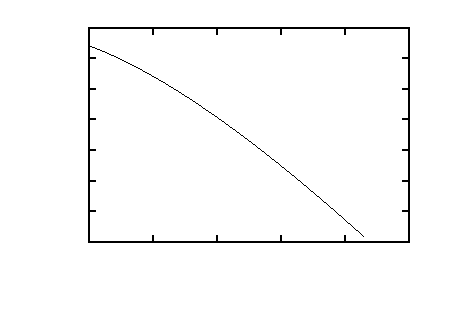
\includegraphics{chNucParamsEPfp}}%
    \gplfronttext
  \end{picture}%
\endgroup
}\\
%  \subfloat[d pfp]{\input{\missingfigure{sigma_water}}}
%  \subfloat[e pfp]{\input{\missingfigure{sigma_pfp}}}
%     \subfloat[]{
%     \missingfigure{The sketch of the arrangement}\label{fig:pressure_pulses:a}
%   }\\
  \caption{
    A plot of the  temperature dependence of the parameters $d$ and $\epsilon$ 
    in the hard-sphere model with Lennard-Jones interactions.
  }
 \label{fig:nuc:params}
\end{figure}

\subsubsection{The coexistence curve}

The coexistence curve for water and perfluoropentane are plotted in \figref{nuc:coex}.
The experimental values that are used to make the fit are shown with points,
and the computed curve is shown with a solid line.  
The fit for the vapour was  used to obtain $d$ and $\epsilon$ for the model and so is by definition exact.
The quality of the model can be assessed by comparing the experimental values for the liquid with the fit.
It is seen to be highly accurate away from the critical point, 
at which point theory and experiment start to diverge.


The calculated spinodal is also plotted in \figref{nuc:coex}.
The spinodal is defines the point of equilibrium where the energy barrier to the transition vanishes (see Favvas\cite{Favvas2008} for an introduction).
There region of the spinodal is bound by the curves
\sub{
\label{eqn:LocusSpinodal}
\begin{align}
  \mu_v = \mu_\hs(\rho_v) - \alpha \rho_v &= \mu_\hs(\rho_L) - \alpha \rho_L = \mu_L,\label{eqn:Locus0}\\
  \frac{\d \mu_v}{\d \rho} &= 0 \label{eqn:Locus1}\\
\text{or}\quad  \frac{\d \mu_L}{\d \rho} &= 0 \label{eqn:Locus2} 
\end{align}
}
Equation  \eqnref{Locus0} demands thermodynamic equilibrium.
Equation \eqnref{Locus1}  ad  \eqnref{Locus2}  demand that the equilibrium point is a saddle point (where the energy barrier vanishes).
%
%In addition to the nucleation rate we provide an upper bound on the pressure required to induce a phase change.
%The spinodal provide an upper bound on the pressure required to induce a phase change.
While the decomposition of phases past the spinodal is not  nucleation -
the phases separate throughout the medium rather than forming a bubble -
the spinodal nevertheless marks a fundamental and guaranteed  change in the medium that is surely detectable.
%It is seen that at \unit{20}\degree\ perfluoropentane will undergo a phase change at ....

The fitted values of $d$ and $epsilon$ are plotted in \figref{nuc:params}.
The stability of the parameters below the critical point is encouraging
for it indicates that the predictive power of the parameters is strong.
Near the critical point the curve in 
starting to be very sensitive changes in temperature.
The model is not applicable near the critical point 
and its parameters are being pulled inappropriately by the changing 
physics.
%interactions In this domain the parameters are having 
%The parameters are b
%for it would surely indicate a failure in the model if the characteristic energy and distance 
%varied too strongly.


\ctable[cap=Density functional parameters,
        caption=Density functional parameters for perfluoropentane and water at \unit{20}\degree,
        label=table:nuc:fitparams,
        pos=top,
        %width = 0.6\textwidth,
        left
       ]
       {llrrc}
{
}{\FL
  &        & \pfp & water & 
    \ML
    &$\epsilon$  & -80 zJ &    -76 zJ   &
    \NN
    &$d$ &  \unit{0.61}\nano\metre &  \unit{0.31}\nano\metre  &
    \NN
    &$\sigma$  &  \unit{0.41}\nano\metre& \unit{0.016}\nano\metre    &   
    \LL
  }

\begin{figure}
 \centering 
  \subfloat[Density profile at the interface of water]{\label{nuc:profiles:water}% GNUPLOT: LaTeX picture with Postscript
\begingroup
  \makeatletter
  \providecommand\color[2][]{%
    \GenericError{(gnuplot) \space\space\space\@spaces}{%
      Package color not loaded in conjunction with
      terminal option `colourtext'%
    }{See the gnuplot documentation for explanation.%
    }{Either use 'blacktext' in gnuplot or load the package
      color.sty in LaTeX.}%
    \renewcommand\color[2][]{}%
  }%
  \providecommand\includegraphics[2][]{%
    \GenericError{(gnuplot) \space\space\space\@spaces}{%
      Package graphicx or graphics not loaded%
    }{See the gnuplot documentation for explanation.%
    }{The gnuplot epslatex terminal needs graphicx.sty or graphics.sty.}%
    \renewcommand\includegraphics[2][]{}%
  }%
  \providecommand\rotatebox[2]{#2}%
  \@ifundefined{ifGPcolor}{%
    \newif\ifGPcolor
    \GPcolorfalse
  }{}%
  \@ifundefined{ifGPblacktext}{%
    \newif\ifGPblacktext
    \GPblacktexttrue
  }{}%
  % define a \g@addto@macro without @ in the name:
  \let\gplgaddtomacro\g@addto@macro
  % define empty templates for all commands taking text:
  \gdef\gplbacktext{}%
  \gdef\gplfronttext{}%
  \makeatother
  \ifGPblacktext
    % no textcolor at all
    \def\colorrgb#1{}%
    \def\colorgray#1{}%
  \else
    % gray or color?
    \ifGPcolor
      \def\colorrgb#1{\color[rgb]{#1}}%
      \def\colorgray#1{\color[gray]{#1}}%
      \expandafter\def\csname LTw\endcsname{\color{white}}%
      \expandafter\def\csname LTb\endcsname{\color{black}}%
      \expandafter\def\csname LTa\endcsname{\color{black}}%
      \expandafter\def\csname LT0\endcsname{\color[rgb]{1,0,0}}%
      \expandafter\def\csname LT1\endcsname{\color[rgb]{0,1,0}}%
      \expandafter\def\csname LT2\endcsname{\color[rgb]{0,0,1}}%
      \expandafter\def\csname LT3\endcsname{\color[rgb]{1,0,1}}%
      \expandafter\def\csname LT4\endcsname{\color[rgb]{0,1,1}}%
      \expandafter\def\csname LT5\endcsname{\color[rgb]{1,1,0}}%
      \expandafter\def\csname LT6\endcsname{\color[rgb]{0,0,0}}%
      \expandafter\def\csname LT7\endcsname{\color[rgb]{1,0.3,0}}%
      \expandafter\def\csname LT8\endcsname{\color[rgb]{0.5,0.5,0.5}}%
    \else
      % gray
      \def\colorrgb#1{\color{black}}%
      \def\colorgray#1{\color[gray]{#1}}%
      \expandafter\def\csname LTw\endcsname{\color{white}}%
      \expandafter\def\csname LTb\endcsname{\color{black}}%
      \expandafter\def\csname LTa\endcsname{\color{black}}%
      \expandafter\def\csname LT0\endcsname{\color{black}}%
      \expandafter\def\csname LT1\endcsname{\color{black}}%
      \expandafter\def\csname LT2\endcsname{\color{black}}%
      \expandafter\def\csname LT3\endcsname{\color{black}}%
      \expandafter\def\csname LT4\endcsname{\color{black}}%
      \expandafter\def\csname LT5\endcsname{\color{black}}%
      \expandafter\def\csname LT6\endcsname{\color{black}}%
      \expandafter\def\csname LT7\endcsname{\color{black}}%
      \expandafter\def\csname LT8\endcsname{\color{black}}%
    \fi
  \fi
  \setlength{\unitlength}{0.0500bp}%
  \begin{picture}(5760.00,4032.00)%
    \gplgaddtomacro\gplbacktext{%
      \csname LTb\endcsname%
      \put(814,704){\makebox(0,0)[r]{\strut{} 0}}%
      \put(814,1142){\makebox(0,0)[r]{\strut{} 5}}%
      \put(814,1579){\makebox(0,0)[r]{\strut{} 10}}%
      \put(814,2017){\makebox(0,0)[r]{\strut{} 15}}%
      \put(814,2454){\makebox(0,0)[r]{\strut{} 20}}%
      \put(814,2892){\makebox(0,0)[r]{\strut{} 25}}%
      \put(814,3329){\makebox(0,0)[r]{\strut{} 30}}%
      \put(814,3767){\makebox(0,0)[r]{\strut{} 35}}%
      \put(946,484){\makebox(0,0){\strut{}-4}}%
      \put(1498,484){\makebox(0,0){\strut{}-3}}%
      \put(2050,484){\makebox(0,0){\strut{}-2}}%
      \put(2602,484){\makebox(0,0){\strut{}-1}}%
      \put(3155,484){\makebox(0,0){\strut{} 0}}%
      \put(3707,484){\makebox(0,0){\strut{} 1}}%
      \put(4259,484){\makebox(0,0){\strut{} 2}}%
      \put(4811,484){\makebox(0,0){\strut{} 3}}%
      \put(5363,484){\makebox(0,0){\strut{} 4}}%
      \put(176,2235){\rotatebox{-270}{\makebox(0,0){\strut{}number density ($nm^{-3}$)}}}%
      \put(3154,154){\makebox(0,0){\strut{}distance ($nm$)}}%
    }%
    \gplgaddtomacro\gplfronttext{%
      \csname LTb\endcsname%
      \put(2266,3594){\makebox(0,0)[r]{\strut{}water}}%
      \csname LTb\endcsname%
      \put(2266,3374){\makebox(0,0)[r]{\strut{}capillary}}%
    }%
    \gplbacktext
    \put(0,0){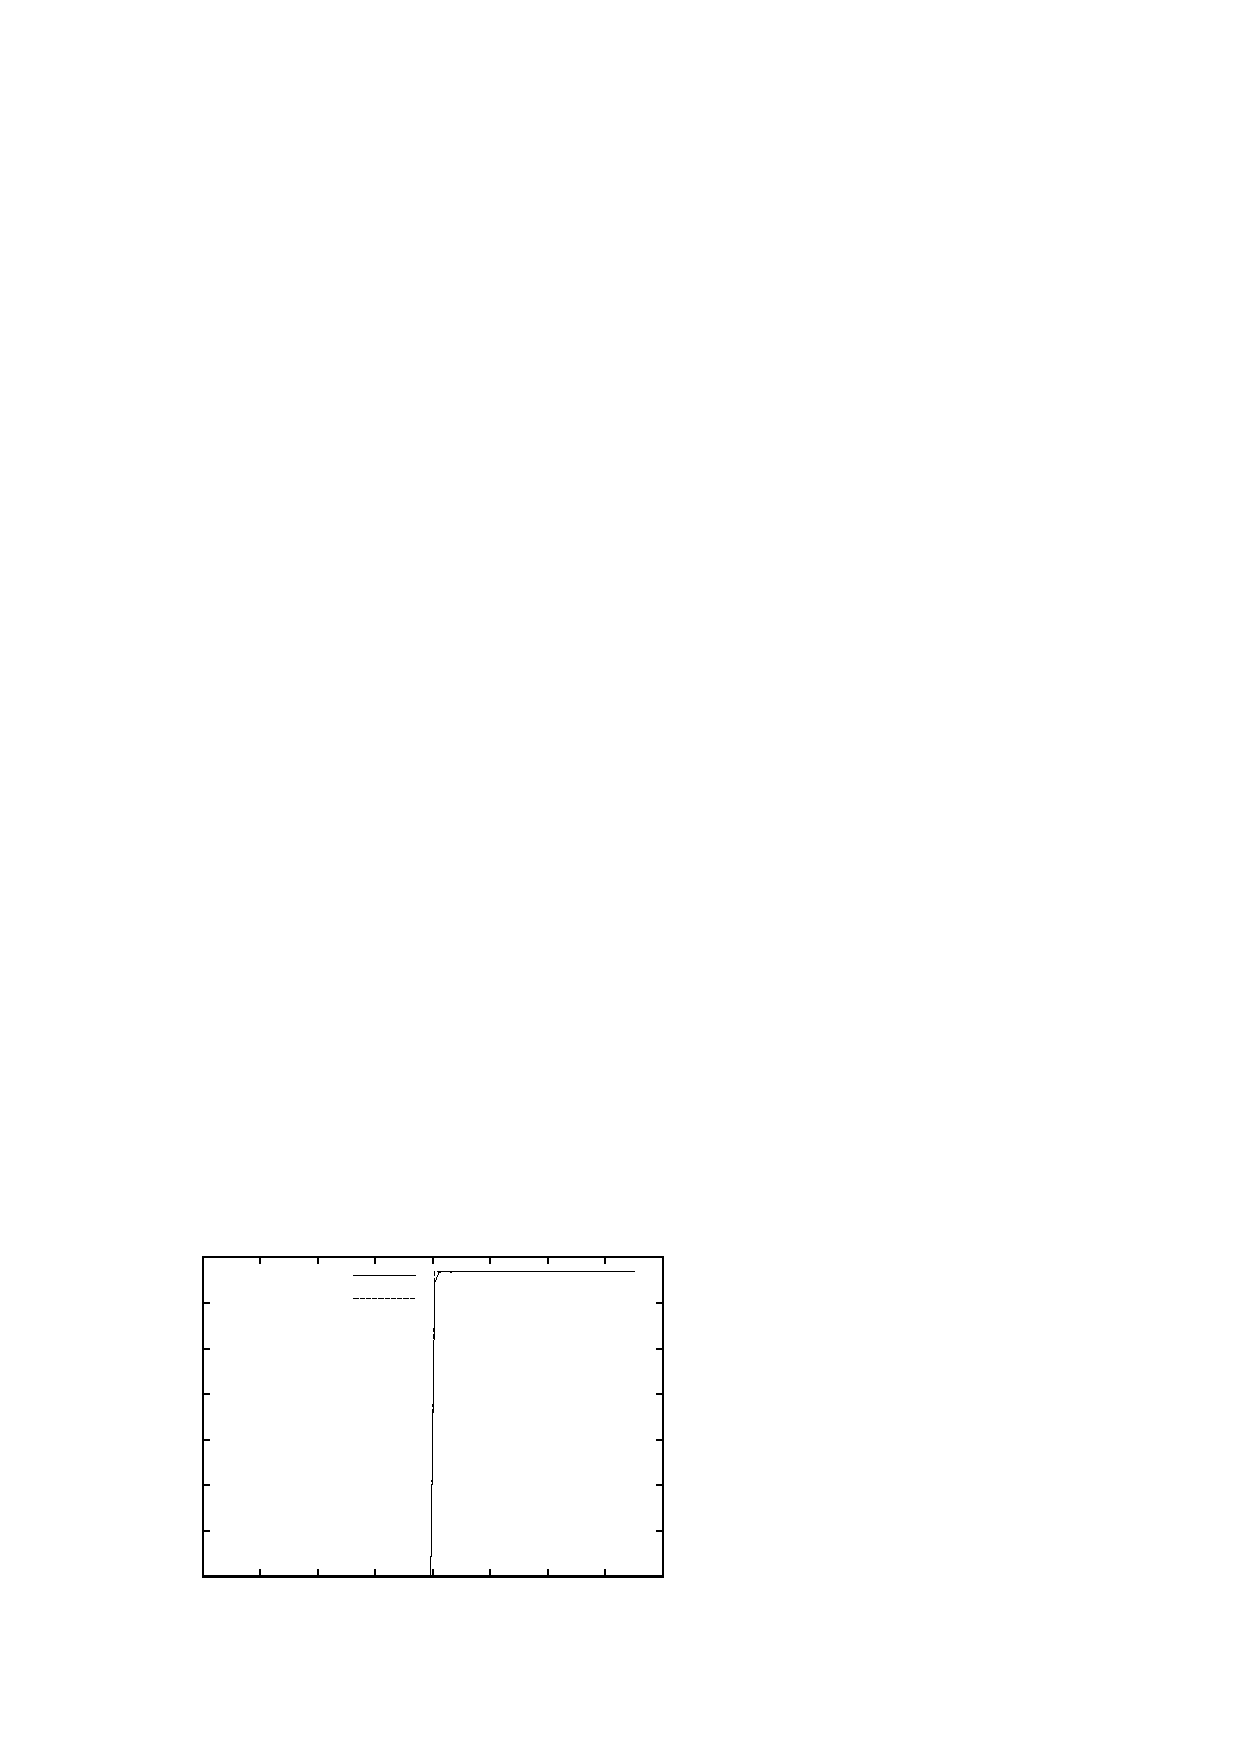
\includegraphics{profile_water}}%
    \gplfronttext
  \end{picture}%
\endgroup
}\\
  \subfloat[Density profile at the interface of \pfp]{\label{nuc:profiles:pfp}% GNUPLOT: LaTeX picture with Postscript
\begingroup
  \makeatletter
  \providecommand\color[2][]{%
    \GenericError{(gnuplot) \space\space\space\@spaces}{%
      Package color not loaded in conjunction with
      terminal option `colourtext'%
    }{See the gnuplot documentation for explanation.%
    }{Either use 'blacktext' in gnuplot or load the package
      color.sty in LaTeX.}%
    \renewcommand\color[2][]{}%
  }%
  \providecommand\includegraphics[2][]{%
    \GenericError{(gnuplot) \space\space\space\@spaces}{%
      Package graphicx or graphics not loaded%
    }{See the gnuplot documentation for explanation.%
    }{The gnuplot epslatex terminal needs graphicx.sty or graphics.sty.}%
    \renewcommand\includegraphics[2][]{}%
  }%
  \providecommand\rotatebox[2]{#2}%
  \@ifundefined{ifGPcolor}{%
    \newif\ifGPcolor
    \GPcolorfalse
  }{}%
  \@ifundefined{ifGPblacktext}{%
    \newif\ifGPblacktext
    \GPblacktexttrue
  }{}%
  % define a \g@addto@macro without @ in the name:
  \let\gplgaddtomacro\g@addto@macro
  % define empty templates for all commands taking text:
  \gdef\gplbacktext{}%
  \gdef\gplfronttext{}%
  \makeatother
  \ifGPblacktext
    % no textcolor at all
    \def\colorrgb#1{}%
    \def\colorgray#1{}%
  \else
    % gray or color?
    \ifGPcolor
      \def\colorrgb#1{\color[rgb]{#1}}%
      \def\colorgray#1{\color[gray]{#1}}%
      \expandafter\def\csname LTw\endcsname{\color{white}}%
      \expandafter\def\csname LTb\endcsname{\color{black}}%
      \expandafter\def\csname LTa\endcsname{\color{black}}%
      \expandafter\def\csname LT0\endcsname{\color[rgb]{1,0,0}}%
      \expandafter\def\csname LT1\endcsname{\color[rgb]{0,1,0}}%
      \expandafter\def\csname LT2\endcsname{\color[rgb]{0,0,1}}%
      \expandafter\def\csname LT3\endcsname{\color[rgb]{1,0,1}}%
      \expandafter\def\csname LT4\endcsname{\color[rgb]{0,1,1}}%
      \expandafter\def\csname LT5\endcsname{\color[rgb]{1,1,0}}%
      \expandafter\def\csname LT6\endcsname{\color[rgb]{0,0,0}}%
      \expandafter\def\csname LT7\endcsname{\color[rgb]{1,0.3,0}}%
      \expandafter\def\csname LT8\endcsname{\color[rgb]{0.5,0.5,0.5}}%
    \else
      % gray
      \def\colorrgb#1{\color{black}}%
      \def\colorgray#1{\color[gray]{#1}}%
      \expandafter\def\csname LTw\endcsname{\color{white}}%
      \expandafter\def\csname LTb\endcsname{\color{black}}%
      \expandafter\def\csname LTa\endcsname{\color{black}}%
      \expandafter\def\csname LT0\endcsname{\color{black}}%
      \expandafter\def\csname LT1\endcsname{\color{black}}%
      \expandafter\def\csname LT2\endcsname{\color{black}}%
      \expandafter\def\csname LT3\endcsname{\color{black}}%
      \expandafter\def\csname LT4\endcsname{\color{black}}%
      \expandafter\def\csname LT5\endcsname{\color{black}}%
      \expandafter\def\csname LT6\endcsname{\color{black}}%
      \expandafter\def\csname LT7\endcsname{\color{black}}%
      \expandafter\def\csname LT8\endcsname{\color{black}}%
    \fi
  \fi
  \setlength{\unitlength}{0.0500bp}%
  \begin{picture}(5760.00,4032.00)%
    \gplgaddtomacro\gplbacktext{%
      \csname LTb\endcsname%
      \put(946,704){\makebox(0,0)[r]{\strut{} 0}}%
      \put(946,1044){\makebox(0,0)[r]{\strut{} 0.5}}%
      \put(946,1385){\makebox(0,0)[r]{\strut{} 1}}%
      \put(946,1725){\makebox(0,0)[r]{\strut{} 1.5}}%
      \put(946,2065){\makebox(0,0)[r]{\strut{} 2}}%
      \put(946,2406){\makebox(0,0)[r]{\strut{} 2.5}}%
      \put(946,2746){\makebox(0,0)[r]{\strut{} 3}}%
      \put(946,3086){\makebox(0,0)[r]{\strut{} 3.5}}%
      \put(946,3427){\makebox(0,0)[r]{\strut{} 4}}%
      \put(946,3767){\makebox(0,0)[r]{\strut{} 4.5}}%
      \put(1078,484){\makebox(0,0){\strut{}-4}}%
      \put(1614,484){\makebox(0,0){\strut{}-3}}%
      \put(2149,484){\makebox(0,0){\strut{}-2}}%
      \put(2685,484){\makebox(0,0){\strut{}-1}}%
      \put(3221,484){\makebox(0,0){\strut{} 0}}%
      \put(3756,484){\makebox(0,0){\strut{} 1}}%
      \put(4292,484){\makebox(0,0){\strut{} 2}}%
      \put(4827,484){\makebox(0,0){\strut{} 3}}%
      \put(5363,484){\makebox(0,0){\strut{} 4}}%
      \put(176,2235){\rotatebox{-270}{\makebox(0,0){\strut{}number density ($nm^{-3}$)}}}%
      \put(3220,154){\makebox(0,0){\strut{}distance ($nm$)}}%
    }%
    \gplgaddtomacro\gplfronttext{%
      \csname LTb\endcsname%
      \put(2398,3594){\makebox(0,0)[r]{\strut{}pfp}}%
      \csname LTb\endcsname%
      \put(2398,3374){\makebox(0,0)[r]{\strut{}capillary}}%
    }%
    \gplbacktext
    \put(0,0){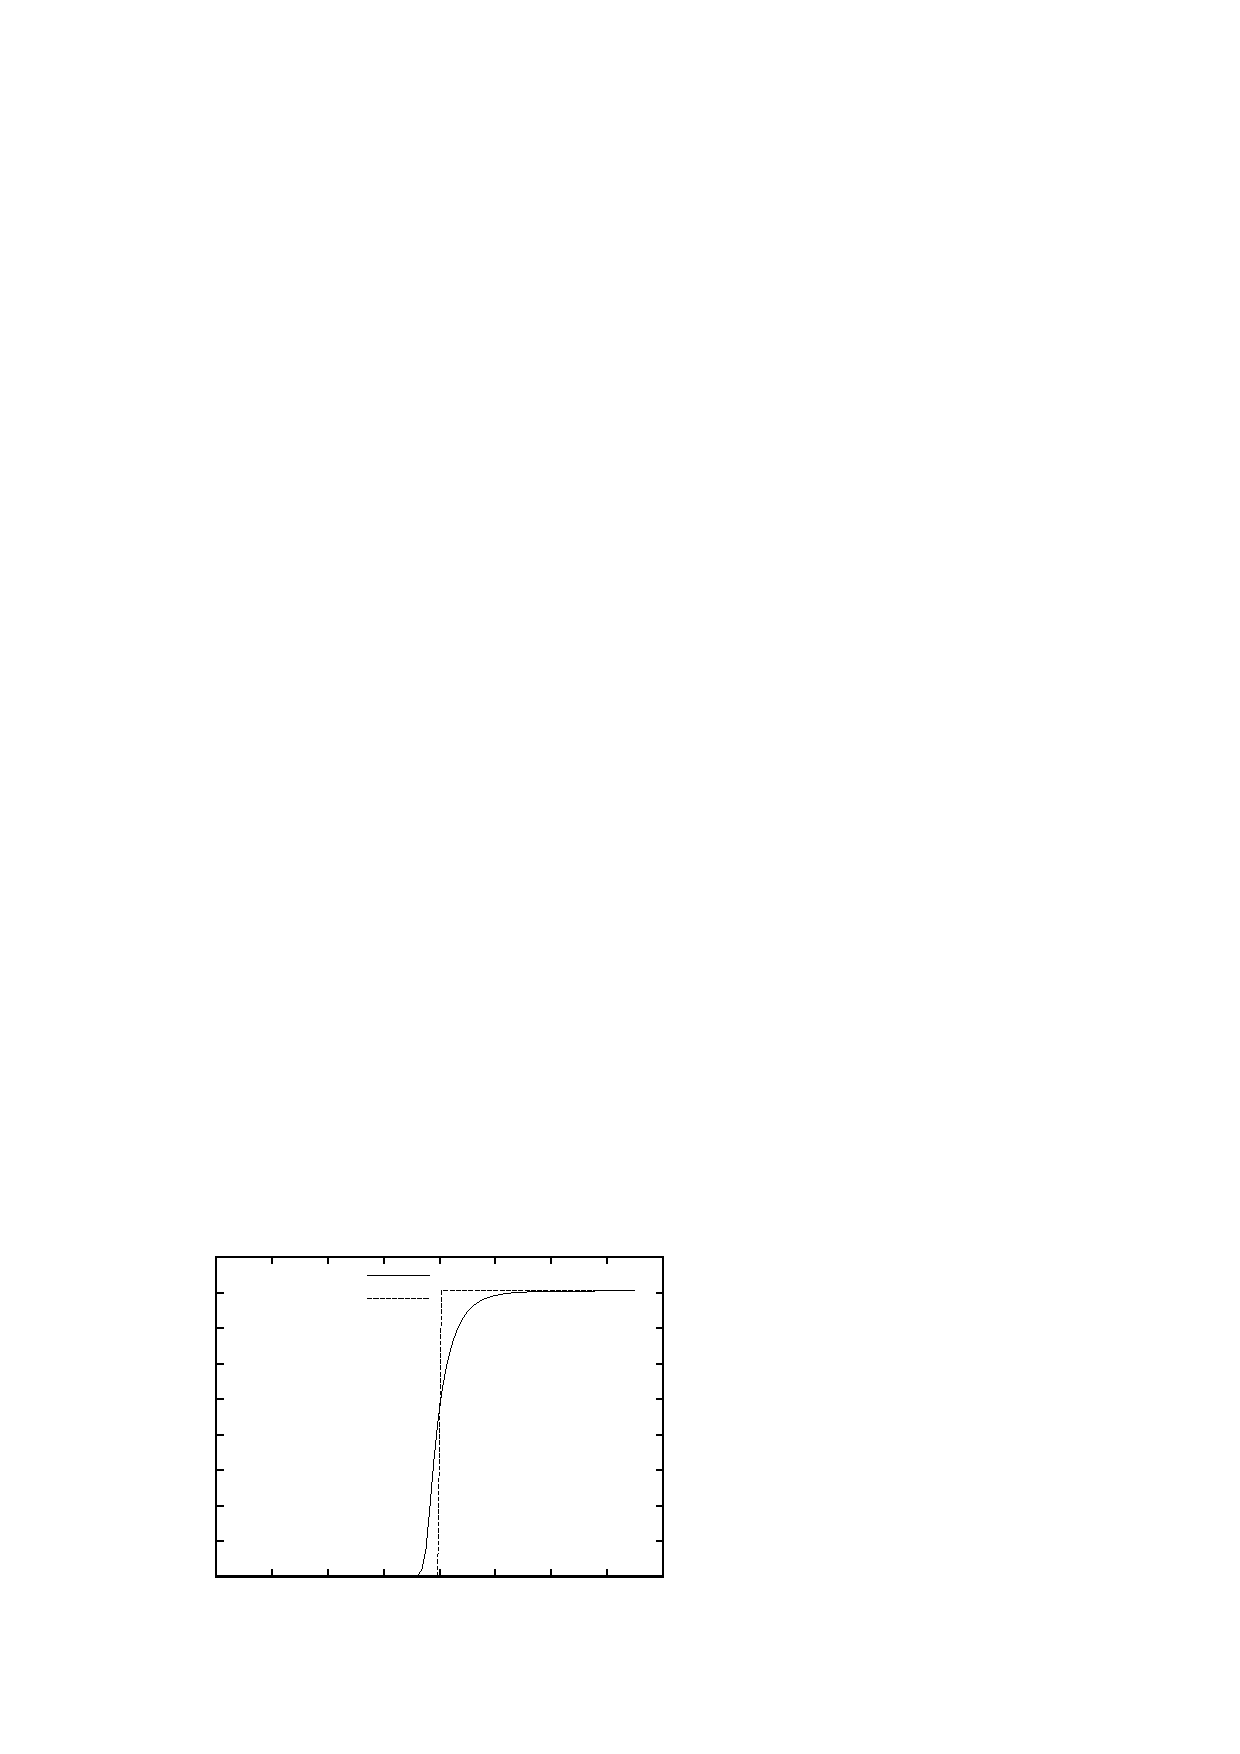
\includegraphics{profile_pfp}}%
    \gplfronttext
  \end{picture}%
\endgroup
}
\caption{
    The plainer density profiles of water and perfluoropentane at \unit{293}\kelvin.
  }
 \label{fig:nuc:profiles}
\end{figure}



The parameters at \unit{20}\degree\ are plotted in \tabref{nuc:fitparams}.
One notable observation is that the distance scale in the Lennard-Jones model is very small for water.
This indicates a very low interaction length. %, which is illustrated in \figref{nuc:LennardJones}.
The reason for this is the highly polar nature of water.
Density functional approaches have previously been found to struggle in the presence of highly polar fluids such as water\cite{Talanquer2001, Nyquist1995},
with the same consequence for the value of $d$.

In \figref{nuc:profiles}
the density profiles for water and perfluoropentane are plotted.
The small value of $d$ for water means that the 
density profile varies over very rapidly 
and is essentially indistinguishable from the apillary approximation.
The are box expected to perform equally poorly.

From \figref{nuc:profiles:pfp} it is seen that the density profile for \pfp\ varies over a more significant length scale.
The \unit{1}\nano\metre\ of \figref{nuc:profiles:pfp} represents approximately 10\%
of the critical radius of a \pfp\ vapour droplet under \unit{1}\mega\pascal\ tension.
The use of the  capillary approximation for \pfp\ is therefore highly questionable.








%However, Talanquer and Oxtoby used dissolved gasses such as oxygen and carbon dioxide as their examples of nucleation. 
%The high vapour pressures of these gases causes the critical radius of the bubble very small: just a few na
%with a corresponding  cause considered  the nucleation of highly volatile liquids  the nucleaton of volatile liquids 

%Such spectacular deviations are typical for bubble nucleation predictions. 
%On the other hand, for predicting the condensation of a vapour bubble 
%\cnt\ is often satisfactory.
%The density functional approach explained this discrepancy by finding that the 
%spinodal exerts a stronger influence on the liquid-vapour transition than its reverse\cite{Oxtoby1997}.
%\Cnt\ does not model the spinodal and the rates predicted for   evaporation and condensation are identical.
%The qualitative success of the classical theory for this transition was considered fortuitous,
%resulting from a cancellation of errors\cite{Oxtoby1997}.

%Talanquer and Oxtoby, however,



%\subsubsection{The density profile}

%\subsection{Evaluation of the Capillary approximation}

\subsection{Further work}
The density profile of \pfp\ plotted in \figref{nuc:profiles:pfp}
indicates that the density functional approach may 
have much to offer theoretical studies of perfluoropentane.

In particular, the density functional approach can be
extended to binary fluids\cite{Talanquer2001} to estimate the nucleation rates for various 
gases dissolved within the perfluorpentane droplet.
The perfluorocarbons are remarkable for their solubility of carbon dioxide.
It could be that type 1  nucleation can be facilitated by the perfluorocarbons  
not by  their low boiling points,
but rather due to the nucleation of their dissolved gases.
%of the medium, but due to the ease with which their solutes form 

%  (using the coexistence value of $\mu$)

%which is plotted in \figref{sppressure}
% Below the critical temperature two phases exist and so the simultaneous  equations \eqnref{BulkCoex} can be solved numerically 
% so long as  $p_\hs(rho)$ and $\mu(\rho)$ are known functions of $\rho$.
% The solutions to \eqnref{BulkCoex} as a function of temperature define the coexistance curve.
%Each minima 

%There is a degree of ambiguity as to what the choice of $d$ should be.
%One choice could be hard sphere diameter of the Kihira model.
%However, as seen from \figref{Kihira_d}, 
%this choice seems unrepresentatively small.
%A more appropriate looking choice seems to be the characteristic length $\sigma$.

%To overcome this difficulty the data is fitted to the


% \begin{figure}
%  \centering
% %\hspace*{-0.2cm}
% % \label{fig:Kihira_potentials}
%  \subfloat[Kihira 2-particle potentials for various perfluorocarbons]{
%   % GNUPLOT: LaTeX picture with Postscript
\begingroup
  \makeatletter
  \providecommand\color[2][]{%
    \GenericError{(gnuplot) \space\space\space\@spaces}{%
      Package color not loaded in conjunction with
      terminal option `colourtext'%
    }{See the gnuplot documentation for explanation.%
    }{Either use 'blacktext' in gnuplot or load the package
      color.sty in LaTeX.}%
    \renewcommand\color[2][]{}%
  }%
  \providecommand\includegraphics[2][]{%
    \GenericError{(gnuplot) \space\space\space\@spaces}{%
      Package graphicx or graphics not loaded%
    }{See the gnuplot documentation for explanation.%
    }{The gnuplot epslatex terminal needs graphicx.sty or graphics.sty.}%
    \renewcommand\includegraphics[2][]{}%
  }%
  \providecommand\rotatebox[2]{#2}%
  \@ifundefined{ifGPcolor}{%
    \newif\ifGPcolor
    \GPcolorfalse
  }{}%
  \@ifundefined{ifGPblacktext}{%
    \newif\ifGPblacktext
    \GPblacktexttrue
  }{}%
  % define a \g@addto@macro without @ in the name:
  \let\gplgaddtomacro\g@addto@macro
  % define empty templates for all commands taking text:
  \gdef\gplbacktext{}%
  \gdef\gplfronttext{}%
  \makeatother
  \ifGPblacktext
    % no textcolor at all
    \def\colorrgb#1{}%
    \def\colorgray#1{}%
  \else
    % gray or color?
    \ifGPcolor
      \def\colorrgb#1{\color[rgb]{#1}}%
      \def\colorgray#1{\color[gray]{#1}}%
      \expandafter\def\csname LTw\endcsname{\color{white}}%
      \expandafter\def\csname LTb\endcsname{\color{black}}%
      \expandafter\def\csname LTa\endcsname{\color{black}}%
      \expandafter\def\csname LT0\endcsname{\color[rgb]{1,0,0}}%
      \expandafter\def\csname LT1\endcsname{\color[rgb]{0,1,0}}%
      \expandafter\def\csname LT2\endcsname{\color[rgb]{0,0,1}}%
      \expandafter\def\csname LT3\endcsname{\color[rgb]{1,0,1}}%
      \expandafter\def\csname LT4\endcsname{\color[rgb]{0,1,1}}%
      \expandafter\def\csname LT5\endcsname{\color[rgb]{1,1,0}}%
      \expandafter\def\csname LT6\endcsname{\color[rgb]{0,0,0}}%
      \expandafter\def\csname LT7\endcsname{\color[rgb]{1,0.3,0}}%
      \expandafter\def\csname LT8\endcsname{\color[rgb]{0.5,0.5,0.5}}%
    \else
      % gray
      \def\colorrgb#1{\color{black}}%
      \def\colorgray#1{\color[gray]{#1}}%
      \expandafter\def\csname LTw\endcsname{\color{white}}%
      \expandafter\def\csname LTb\endcsname{\color{black}}%
      \expandafter\def\csname LTa\endcsname{\color{black}}%
      \expandafter\def\csname LT0\endcsname{\color{black}}%
      \expandafter\def\csname LT1\endcsname{\color{black}}%
      \expandafter\def\csname LT2\endcsname{\color{black}}%
      \expandafter\def\csname LT3\endcsname{\color{black}}%
      \expandafter\def\csname LT4\endcsname{\color{black}}%
      \expandafter\def\csname LT5\endcsname{\color{black}}%
      \expandafter\def\csname LT6\endcsname{\color{black}}%
      \expandafter\def\csname LT7\endcsname{\color{black}}%
      \expandafter\def\csname LT8\endcsname{\color{black}}%
    \fi
  \fi
  \setlength{\unitlength}{0.0500bp}%
  \begin{picture}(5040.00,3528.00)%
    \gplgaddtomacro\gplbacktext{%
      \csname LTb\endcsname%
      \put(1210,704){\makebox(0,0)[r]{\strut{} 0}}%
      \put(1210,1070){\makebox(0,0)[r]{\strut{} 0.5}}%
      \put(1210,1435){\makebox(0,0)[r]{\strut{} 1}}%
      \put(1210,1801){\makebox(0,0)[r]{\strut{} 1.5}}%
      \put(1210,2167){\makebox(0,0)[r]{\strut{} 2}}%
      \put(1210,2533){\makebox(0,0)[r]{\strut{} 2.5}}%
      \put(1210,2898){\makebox(0,0)[r]{\strut{} 3}}%
      \put(1210,3264){\makebox(0,0)[r]{\strut{} 3.5}}%
      \put(1342,484){\makebox(0,0){\strut{} 200}}%
      \put(1791,484){\makebox(0,0){\strut{} 220}}%
      \put(2240,484){\makebox(0,0){\strut{} 240}}%
      \put(2689,484){\makebox(0,0){\strut{} 260}}%
      \put(3138,484){\makebox(0,0){\strut{} 280}}%
      \put(3587,484){\makebox(0,0){\strut{} 300}}%
      \put(4036,484){\makebox(0,0){\strut{} 320}}%
      \put(4485,484){\makebox(0,0){\strut{} 340}}%
      \put(440,1984){\rotatebox{90}{\makebox(0,0){\strut{}vapour pressure, atm}}}%
      \put(3026,154){\makebox(0,0){\strut{}temperature, K}}%
    }%
    \gplgaddtomacro\gplfronttext{%
      \csname LTb\endcsname%
      \put(3058,3091){\makebox(0,0)[r]{\strut{}fit}}%
      \csname LTb\endcsname%
      \put(3058,2871){\makebox(0,0)[r]{\strut{}Barber 1955}}%
      \csname LTb\endcsname%
      \put(3058,2651){\makebox(0,0)[r]{\strut{}Crowder 1967}}%
    }%
    \gplbacktext
    \put(0,0){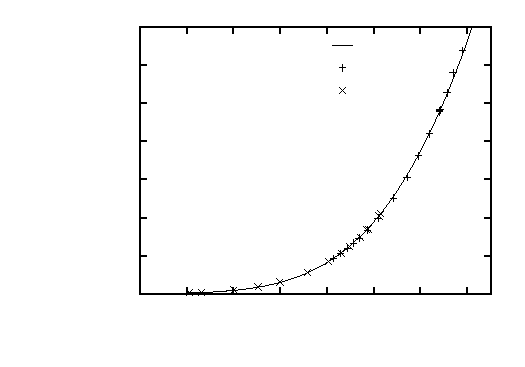
\includegraphics{c2_vapour_pressure_fit}}%
    \gplfronttext
  \end{picture}%
\endgroup
}
% \hfill
% % \label{fig:Kihira_WCA}
%  \subfloat[WCA decomposition of the Kihira  potential for perfluoropentane]{
%   % GNUPLOT: LaTeX picture with Postscript
\begingroup
  \makeatletter
  \providecommand\color[2][]{%
    \GenericError{(gnuplot) \space\space\space\@spaces}{%
      Package color not loaded in conjunction with
      terminal option `colourtext'%
    }{See the gnuplot documentation for explanation.%
    }{Either use 'blacktext' in gnuplot or load the package
      color.sty in LaTeX.}%
    \renewcommand\color[2][]{}%
  }%
  \providecommand\includegraphics[2][]{%
    \GenericError{(gnuplot) \space\space\space\@spaces}{%
      Package graphicx or graphics not loaded%
    }{See the gnuplot documentation for explanation.%
    }{The gnuplot epslatex terminal needs graphicx.sty or graphics.sty.}%
    \renewcommand\includegraphics[2][]{}%
  }%
  \providecommand\rotatebox[2]{#2}%
  \@ifundefined{ifGPcolor}{%
    \newif\ifGPcolor
    \GPcolorfalse
  }{}%
  \@ifundefined{ifGPblacktext}{%
    \newif\ifGPblacktext
    \GPblacktexttrue
  }{}%
  % define a \g@addto@macro without @ in the name:
  \let\gplgaddtomacro\g@addto@macro
  % define empty templates for all commands taking text:
  \gdef\gplbacktext{}%
  \gdef\gplfronttext{}%
  \makeatother
  \ifGPblacktext
    % no textcolor at all
    \def\colorrgb#1{}%
    \def\colorgray#1{}%
  \else
    % gray or color?
    \ifGPcolor
      \def\colorrgb#1{\color[rgb]{#1}}%
      \def\colorgray#1{\color[gray]{#1}}%
      \expandafter\def\csname LTw\endcsname{\color{white}}%
      \expandafter\def\csname LTb\endcsname{\color{black}}%
      \expandafter\def\csname LTa\endcsname{\color{black}}%
      \expandafter\def\csname LT0\endcsname{\color[rgb]{1,0,0}}%
      \expandafter\def\csname LT1\endcsname{\color[rgb]{0,1,0}}%
      \expandafter\def\csname LT2\endcsname{\color[rgb]{0,0,1}}%
      \expandafter\def\csname LT3\endcsname{\color[rgb]{1,0,1}}%
      \expandafter\def\csname LT4\endcsname{\color[rgb]{0,1,1}}%
      \expandafter\def\csname LT5\endcsname{\color[rgb]{1,1,0}}%
      \expandafter\def\csname LT6\endcsname{\color[rgb]{0,0,0}}%
      \expandafter\def\csname LT7\endcsname{\color[rgb]{1,0.3,0}}%
      \expandafter\def\csname LT8\endcsname{\color[rgb]{0.5,0.5,0.5}}%
    \else
      % gray
      \def\colorrgb#1{\color{black}}%
      \def\colorgray#1{\color[gray]{#1}}%
      \expandafter\def\csname LTw\endcsname{\color{white}}%
      \expandafter\def\csname LTb\endcsname{\color{black}}%
      \expandafter\def\csname LTa\endcsname{\color{black}}%
      \expandafter\def\csname LT0\endcsname{\color{black}}%
      \expandafter\def\csname LT1\endcsname{\color{black}}%
      \expandafter\def\csname LT2\endcsname{\color{black}}%
      \expandafter\def\csname LT3\endcsname{\color{black}}%
      \expandafter\def\csname LT4\endcsname{\color{black}}%
      \expandafter\def\csname LT5\endcsname{\color{black}}%
      \expandafter\def\csname LT6\endcsname{\color{black}}%
      \expandafter\def\csname LT7\endcsname{\color{black}}%
      \expandafter\def\csname LT8\endcsname{\color{black}}%
    \fi
  \fi
  \setlength{\unitlength}{0.0500bp}%
  \begin{picture}(5040.00,3528.00)%
    \gplgaddtomacro\gplbacktext{%
      \csname LTb\endcsname%
      \put(1210,704){\makebox(0,0)[r]{\strut{} 0}}%
      \put(1210,1070){\makebox(0,0)[r]{\strut{} 0.5}}%
      \put(1210,1435){\makebox(0,0)[r]{\strut{} 1}}%
      \put(1210,1801){\makebox(0,0)[r]{\strut{} 1.5}}%
      \put(1210,2167){\makebox(0,0)[r]{\strut{} 2}}%
      \put(1210,2533){\makebox(0,0)[r]{\strut{} 2.5}}%
      \put(1210,2898){\makebox(0,0)[r]{\strut{} 3}}%
      \put(1210,3264){\makebox(0,0)[r]{\strut{} 3.5}}%
      \put(1342,484){\makebox(0,0){\strut{} 200}}%
      \put(1791,484){\makebox(0,0){\strut{} 220}}%
      \put(2240,484){\makebox(0,0){\strut{} 240}}%
      \put(2689,484){\makebox(0,0){\strut{} 260}}%
      \put(3138,484){\makebox(0,0){\strut{} 280}}%
      \put(3587,484){\makebox(0,0){\strut{} 300}}%
      \put(4036,484){\makebox(0,0){\strut{} 320}}%
      \put(4485,484){\makebox(0,0){\strut{} 340}}%
      \put(440,1984){\rotatebox{90}{\makebox(0,0){\strut{}vapour pressure, atm}}}%
      \put(3026,154){\makebox(0,0){\strut{}temperature, K}}%
    }%
    \gplgaddtomacro\gplfronttext{%
      \csname LTb\endcsname%
      \put(3058,3091){\makebox(0,0)[r]{\strut{}fit}}%
      \csname LTb\endcsname%
      \put(3058,2871){\makebox(0,0)[r]{\strut{}Barber 1955}}%
      \csname LTb\endcsname%
      \put(3058,2651){\makebox(0,0)[r]{\strut{}Crowder 1967}}%
    }%
    \gplbacktext
    \put(0,0){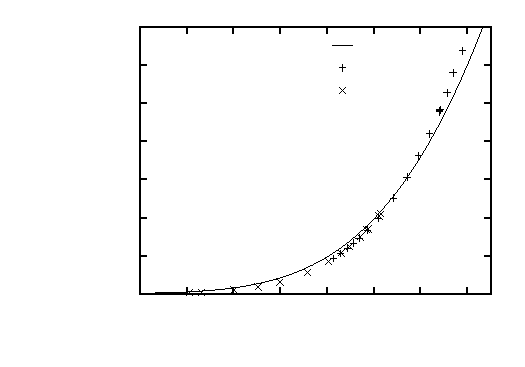
\includegraphics{c2_vapour_pressure_fit_LJ}}%
    \gplfronttext
  \end{picture}%
\endgroup
}\\
% %\label{fig:Kihira_d}
%   \caption{ 
%   }
%  \label{fig:}
% \end{figure}

%The final result of the density functional approach, \figref{profile} shows that the thickness of the interface extends over 10 anstrums on each side of the inteface.
%xsThis is extends over most of the bubble wheWhen this compared to the



% \begin{figure}
%  \centering
% %\hspace*{-0.2cm}
%   % GNUPLOT: LaTeX picture with Postscript
\begingroup
  \makeatletter
  \providecommand\color[2][]{%
    \GenericError{(gnuplot) \space\space\space\@spaces}{%
      Package color not loaded in conjunction with
      terminal option `colourtext'%
    }{See the gnuplot documentation for explanation.%
    }{Either use 'blacktext' in gnuplot or load the package
      color.sty in LaTeX.}%
    \renewcommand\color[2][]{}%
  }%
  \providecommand\includegraphics[2][]{%
    \GenericError{(gnuplot) \space\space\space\@spaces}{%
      Package graphicx or graphics not loaded%
    }{See the gnuplot documentation for explanation.%
    }{The gnuplot epslatex terminal needs graphicx.sty or graphics.sty.}%
    \renewcommand\includegraphics[2][]{}%
  }%
  \providecommand\rotatebox[2]{#2}%
  \@ifundefined{ifGPcolor}{%
    \newif\ifGPcolor
    \GPcolorfalse
  }{}%
  \@ifundefined{ifGPblacktext}{%
    \newif\ifGPblacktext
    \GPblacktexttrue
  }{}%
  % define a \g@addto@macro without @ in the name:
  \let\gplgaddtomacro\g@addto@macro
  % define empty templates for all commands taking text:
  \gdef\gplbacktext{}%
  \gdef\gplfronttext{}%
  \makeatother
  \ifGPblacktext
    % no textcolor at all
    \def\colorrgb#1{}%
    \def\colorgray#1{}%
  \else
    % gray or color?
    \ifGPcolor
      \def\colorrgb#1{\color[rgb]{#1}}%
      \def\colorgray#1{\color[gray]{#1}}%
      \expandafter\def\csname LTw\endcsname{\color{white}}%
      \expandafter\def\csname LTb\endcsname{\color{black}}%
      \expandafter\def\csname LTa\endcsname{\color{black}}%
      \expandafter\def\csname LT0\endcsname{\color[rgb]{1,0,0}}%
      \expandafter\def\csname LT1\endcsname{\color[rgb]{0,1,0}}%
      \expandafter\def\csname LT2\endcsname{\color[rgb]{0,0,1}}%
      \expandafter\def\csname LT3\endcsname{\color[rgb]{1,0,1}}%
      \expandafter\def\csname LT4\endcsname{\color[rgb]{0,1,1}}%
      \expandafter\def\csname LT5\endcsname{\color[rgb]{1,1,0}}%
      \expandafter\def\csname LT6\endcsname{\color[rgb]{0,0,0}}%
      \expandafter\def\csname LT7\endcsname{\color[rgb]{1,0.3,0}}%
      \expandafter\def\csname LT8\endcsname{\color[rgb]{0.5,0.5,0.5}}%
    \else
      % gray
      \def\colorrgb#1{\color{black}}%
      \def\colorgray#1{\color[gray]{#1}}%
      \expandafter\def\csname LTw\endcsname{\color{white}}%
      \expandafter\def\csname LTb\endcsname{\color{black}}%
      \expandafter\def\csname LTa\endcsname{\color{black}}%
      \expandafter\def\csname LT0\endcsname{\color{black}}%
      \expandafter\def\csname LT1\endcsname{\color{black}}%
      \expandafter\def\csname LT2\endcsname{\color{black}}%
      \expandafter\def\csname LT3\endcsname{\color{black}}%
      \expandafter\def\csname LT4\endcsname{\color{black}}%
      \expandafter\def\csname LT5\endcsname{\color{black}}%
      \expandafter\def\csname LT6\endcsname{\color{black}}%
      \expandafter\def\csname LT7\endcsname{\color{black}}%
      \expandafter\def\csname LT8\endcsname{\color{black}}%
    \fi
  \fi
  \setlength{\unitlength}{0.0500bp}%
  \begin{picture}(5040.00,3528.00)%
    \gplgaddtomacro\gplbacktext{%
      \csname LTb\endcsname%
      \put(1606,704){\makebox(0,0)[r]{\strut{} 0}}%
      \put(1606,1070){\makebox(0,0)[r]{\strut{} 0.0005}}%
      \put(1606,1435){\makebox(0,0)[r]{\strut{} 0.001}}%
      \put(1606,1801){\makebox(0,0)[r]{\strut{} 0.0015}}%
      \put(1606,2167){\makebox(0,0)[r]{\strut{} 0.002}}%
      \put(1606,2533){\makebox(0,0)[r]{\strut{} 0.0025}}%
      \put(1606,2898){\makebox(0,0)[r]{\strut{} 0.003}}%
      \put(1606,3264){\makebox(0,0)[r]{\strut{} 0.0035}}%
      \put(1738,484){\makebox(0,0){\strut{} 0}}%
      \put(2233,484){\makebox(0,0){\strut{} 20}}%
      \put(2729,484){\makebox(0,0){\strut{} 40}}%
      \put(3224,484){\makebox(0,0){\strut{} 60}}%
      \put(3719,484){\makebox(0,0){\strut{} 80}}%
      \put(4215,484){\makebox(0,0){\strut{} 100}}%
      \put(4710,484){\makebox(0,0){\strut{} 120}}%
      \put(440,1984){\rotatebox{90}{\makebox(0,0){\strut{}number density}}}%
      \put(3224,154){\makebox(0,0){\strut{}distance, Angstrum}}%
    }%
    \gplgaddtomacro\gplfronttext{%
    }%
    \gplbacktext
    \put(0,0){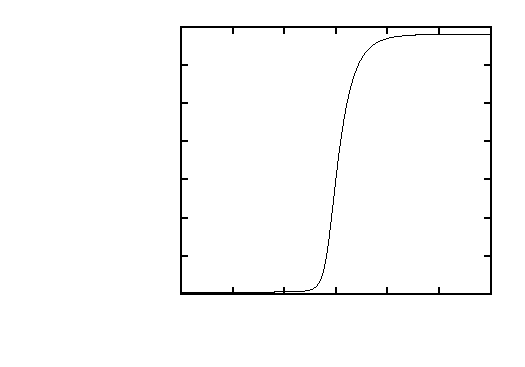
\includegraphics{c2_interface}}%
    \gplfronttext
  \end{picture}%
\endgroup

%   \caption{ The density profile of perfluoropentane at a plainer interface.
%   }
%  \label{fig:profile}
% \end{figure}
% \begin{figure}
%   % GNUPLOT: LaTeX picture with Postscript
\begingroup
  \makeatletter
  \providecommand\color[2][]{%
    \GenericError{(gnuplot) \space\space\space\@spaces}{%
      Package color not loaded in conjunction with
      terminal option `colourtext'%
    }{See the gnuplot documentation for explanation.%
    }{Either use 'blacktext' in gnuplot or load the package
      color.sty in LaTeX.}%
    \renewcommand\color[2][]{}%
  }%
  \providecommand\includegraphics[2][]{%
    \GenericError{(gnuplot) \space\space\space\@spaces}{%
      Package graphicx or graphics not loaded%
    }{See the gnuplot documentation for explanation.%
    }{The gnuplot epslatex terminal needs graphicx.sty or graphics.sty.}%
    \renewcommand\includegraphics[2][]{}%
  }%
  \providecommand\rotatebox[2]{#2}%
  \@ifundefined{ifGPcolor}{%
    \newif\ifGPcolor
    \GPcolorfalse
  }{}%
  \@ifundefined{ifGPblacktext}{%
    \newif\ifGPblacktext
    \GPblacktexttrue
  }{}%
  % define a \g@addto@macro without @ in the name:
  \let\gplgaddtomacro\g@addto@macro
  % define empty templates for all commands taking text:
  \gdef\gplbacktext{}%
  \gdef\gplfronttext{}%
  \makeatother
  \ifGPblacktext
    % no textcolor at all
    \def\colorrgb#1{}%
    \def\colorgray#1{}%
  \else
    % gray or color?
    \ifGPcolor
      \def\colorrgb#1{\color[rgb]{#1}}%
      \def\colorgray#1{\color[gray]{#1}}%
      \expandafter\def\csname LTw\endcsname{\color{white}}%
      \expandafter\def\csname LTb\endcsname{\color{black}}%
      \expandafter\def\csname LTa\endcsname{\color{black}}%
      \expandafter\def\csname LT0\endcsname{\color[rgb]{1,0,0}}%
      \expandafter\def\csname LT1\endcsname{\color[rgb]{0,1,0}}%
      \expandafter\def\csname LT2\endcsname{\color[rgb]{0,0,1}}%
      \expandafter\def\csname LT3\endcsname{\color[rgb]{1,0,1}}%
      \expandafter\def\csname LT4\endcsname{\color[rgb]{0,1,1}}%
      \expandafter\def\csname LT5\endcsname{\color[rgb]{1,1,0}}%
      \expandafter\def\csname LT6\endcsname{\color[rgb]{0,0,0}}%
      \expandafter\def\csname LT7\endcsname{\color[rgb]{1,0.3,0}}%
      \expandafter\def\csname LT8\endcsname{\color[rgb]{0.5,0.5,0.5}}%
    \else
      % gray
      \def\colorrgb#1{\color{black}}%
      \def\colorgray#1{\color[gray]{#1}}%
      \expandafter\def\csname LTw\endcsname{\color{white}}%
      \expandafter\def\csname LTb\endcsname{\color{black}}%
      \expandafter\def\csname LTa\endcsname{\color{black}}%
      \expandafter\def\csname LT0\endcsname{\color{black}}%
      \expandafter\def\csname LT1\endcsname{\color{black}}%
      \expandafter\def\csname LT2\endcsname{\color{black}}%
      \expandafter\def\csname LT3\endcsname{\color{black}}%
      \expandafter\def\csname LT4\endcsname{\color{black}}%
      \expandafter\def\csname LT5\endcsname{\color{black}}%
      \expandafter\def\csname LT6\endcsname{\color{black}}%
      \expandafter\def\csname LT7\endcsname{\color{black}}%
      \expandafter\def\csname LT8\endcsname{\color{black}}%
    \fi
  \fi
  \setlength{\unitlength}{0.0500bp}%
  \begin{picture}(5040.00,3528.00)%
    \gplgaddtomacro\gplbacktext{%
      \csname LTb\endcsname%
      \put(1078,704){\makebox(0,0)[r]{\strut{} 0}}%
      \put(1078,1216){\makebox(0,0)[r]{\strut{} 10}}%
      \put(1078,1728){\makebox(0,0)[r]{\strut{} 20}}%
      \put(1078,2240){\makebox(0,0)[r]{\strut{} 30}}%
      \put(1078,2752){\makebox(0,0)[r]{\strut{} 40}}%
      \put(1078,3264){\makebox(0,0)[r]{\strut{} 50}}%
      \put(1210,484){\makebox(0,0){\strut{} 200}}%
      \put(1910,484){\makebox(0,0){\strut{} 250}}%
      \put(2610,484){\makebox(0,0){\strut{} 300}}%
      \put(3310,484){\makebox(0,0){\strut{} 350}}%
      \put(4010,484){\makebox(0,0){\strut{} 400}}%
      \put(4710,484){\makebox(0,0){\strut{} 450}}%
      \put(440,1984){\rotatebox{90}{\makebox(0,0){\strut{}pressure (MPa)}}}%
      \put(2960,154){\makebox(0,0){\strut{}temperature, K}}%
    }%
    \gplgaddtomacro\gplfronttext{%
    }%
    \gplbacktext
    \put(0,0){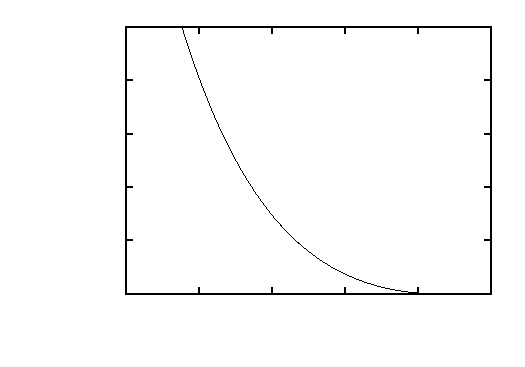
\includegraphics{c2_lspinodal_pressure}}%
    \gplfronttext
  \end{picture}%
\endgroup

%   \caption{ 
%     The pressure difference between coexistance and the liquid spinodal.
% This graph calculates  the pressures required to guarantee a phase change.
% Notice that the pressures required vanish at the critical pressure.
%   }
%  \label{fig:sppressure}
% \end{figure}



% \subsubsection{The Carnarhan-Stirling Hard Sphere Equation of State}


% To make further progress we need to solve the thermodynamics of the reference hard sphere fluid.
% This can be done by starting with the hightly accurate Carnahan-Stirling equaion of state,
% Carnahan-Starling\cite{Carnahan1969} see\cite{Song1989} for interest, equation of state
% \begin{align}
% Z = \frac{pV}{N\kB T} = \frac{1+\eta +\eta^2-\eta^3}{1-\eta^3}\label{eqn:HSeos}
% \end{align}
% where $\eta$ is the packing fraction of the fluid,
% \begin{align}
%   \eta = \eta(\rho) = \frac{\pi \rho d^3}{6}
% \end{align}
% where $d$ is the hard-sphere diameter.

% By rearranging \eqnref{HSeos} the pressure is
% \begin{align}
%   p = \kB T \rho \frac{1+\eta +\eta^2-\eta^3}{1-\eta^3} \label{eqn:HSpressure}
% \end{align}

% To calculate the hard-sphere free energy  it is useful to calcuate the residual pressure over that of an ideal gas.
% That is 
% \begin{align}
% p^\Res = p - p_\ideal = p -\rho\kB T = \rho \kB T \lr{Z-1}.
% \end{align}
% At a constant temperature the residual free energy $df^\Res = - p^\Res dV$ may then be integrated so that
% \begin{align}
%   \fh &= f_\ideal  - p ^\Res dV/V =  f_\ideal  +  \rho \kB T \int_0^\rho d\rho^\prime \frac{\lr{Z-1}}{\rho^\prime }\\
% &=   f_\ideal + \rho \kB T\frac{4\eta - 3\eta^2}{\lr{1-\eta}^2}
% \end{align}
% where the free energy per volume of an ideal gas is\cite{Santos2005}
% \begin{align}
%   f_\ideal =  \rho\kB T\lr{\ln \lr{\rho \lambda^3} -1}. % \sum_i \ln \lr{\rho_i \lambda_i^3} -1.
% \end{align}
% $\lambda$ is the de Broglie wavelenghth of the medium.
% Finally, the chemical potential is 
% \begin{align}
%   \mu = \mu_h + \mu_\ideal = \frac{d \fh}{d \rho} + \mu_\ideal=  \kB T\frac{8\eta - 9 \eta^2 + 3\eta^3}{\lr{1-\eta}^3} + \kB \ln \lr{\rho \lambda^3}
% \end{align}

% excess chemical potential is\cite{Lee1995}
% \begin{align}
% \mu = \kB T\frac{8\eta - 9 \eta^2 + 3\eta^3}{\lr{1-\eta}^3}
% \end{align}
% or should that be\cite{Yang2002}
% \begin{align}
% \mu = \kB T\frac{8\eta - 9 \eta^2 + 3\eta^3}{\lr{1-\eta}^3} - 
% \end{align}
%http://www.sklogwiki.org/SklogWiki/index.php/Carnahan-Starling_equation_of_state



%%% Local Variables: 
%%% mode: latex
%%% TeX-master: "../../tshorrock_thesis"
%%% End: 



\chapter{An acoustic theory of special relativity}\label{ch:acousticSR}


\section{Introduction}\label{sec:AcousticSR:introduction}

The privileged role of light is perhaps the most mysterious aspect of Einstein's special theory of relativity.
What is it about this signal, as opposed to any other method of communication, that makes it  so fundamental to the  concepts of time and space?
The answer, for Einstein, is  that light has a constant speed that  is independent of the motion of the light source\cite{Einstein1905}.
This  property enables the  distance between an observer and a faraway object  to be measured  by determining the to-fro propagation time of a pulse of light.
The measurement is local to the observer and all the observer requires to make the measurement 
 is a light source, a receiver and a clock.
Einstein's definition of measurement is then completed with his principle of relativity,
which demands that a measuring device at rest with respect to an observer, such as a clock or a metre rule, 
gauge quantities that are independent of the observer's motion\cite{Einstein1905, Pierseaux2005}.

In Einstein's  theory the observer does  not need to know their speed relative to the speed of the light medium - the {\em \aether}.
The postulates demand that \aetherial\ motion  neither alters the speed of light
nor alters the units of the measurements used by the observer.
%The second of these restrictions is a consequence of Einstein's  Principle of Relativity,
%which demands that the units of measurement
%Einstein's definition of measurement is then completed with his Principle of Relativity,
%which demands that the units of measurement that are stationary for one observer  as the units at that move uniformly to one another.
%
%and secondly because the \aether\ is assumed not to alter the length of a {\em rigid} measuring device (physical identity of the  units of measure - a consequence of Einstein's relativity  relativity postulate).
The observer can therefore consider \herself to be stationary and not consider the \aether\ at all.
This elimination of the \aether, however, only emphasises the uniqueness of light, for it is the  only  signal that has a  medium with no measurable mechanical properties.
%The central role of light in the measurement process is unsettling. 
%How lucky we are to be born with eyes! 
%Surely otherwise we would not have thought to look for such a signal. %be the only signal that has no measurable medium - no \aether.
Satisfactory definitions of time and space seem to come at the expense of making light  an even greater puzzle,
more and more distant from the world that we can touch and hear.
%We are very fortunate that we can see.
%Would this definition of time and space be satisfactory if we could not?

The relativity theory of \Poincare is different.
%In the relativity theory of \Poincare, on the other hand,
%The relativity theory of \Poincare, on the other hand, neither  eliminates the \aether\ nor 
%postulates the constancy of the speed of light.
%For \Poincare 
For \Poincare, light does have a medium and all motions can be  measured with respect to it;
`stationary' means stationary with respect to the \aether\cite{Poincare1908,PoincareScienceAndMethod,Pierseaux2005}.
Unlike Einstein's theory, the length of a measuring rod used by an observer is affected by the observers motion.
Indeed, \Poincare\ {\em postulates} that it contracts from its  length as measured when stationary with respect to the \aether,
with the size of the contraction  determined by the spatial Lorentz transformation\cite{Poincare1906, Pierseaux2005}.
%\ and
%so there is only one stationary reference.
%This leads to a difference in the  interpretation given to  the Lorentz transformation.
%\Poincare's  Principle of Relativity is also slightly different from Einstein's.
It follows that the principle of relativity  is also different;
\Poincare assumes only that there is no absolute reference from  which to measure the speed of the \aether\cite{Poincare1906}.
However, \Poincare's formulation of special relativity is not at odds with any experimental confirmation of Einstein's theory\cite{Pierseaux2001}.
This is because \Poincare, like Einstein, uses the Lorentz transformations to switch between the spatial-temporal measurements of different observers,
and because both theories are invariant in  the quadratic form;
light does have a constant speed in  \Poincare's theory of relativity\cite{Pierseaux2001}.
Like Einstein, \Poincare recognises that the constancy of the speed of light is a postulate.
In 1898\cite{Poincare1898} he notes that when an astronomer measures the speed of light, 
\blockquote{
  He has begun by supposing that light has a constant velocity, 
  and in particular that its velocity is the same in all directions. 
  That is a postulate without which no measurement of this velocity could be attempted. 
%  This postulate could never be verified directly by experiment; 
%  it might be contradicted by it if the results of different measurements were not concordant.
%  We  should think ourselves fortunate that this contradiction has not happened...
}
However, \Poincare's  theory does not depend upon this postulate,
for \Poincare uses the postulated Lorentz length contraction as an alternative\cite{Pierseaux2005}.
Light is not a privileged signal in \Poincare's theory
but this flexibility is obtained only at the cost of admitting  motion dependant deformations.
A fundamental explanation for these is  missing, however,
and this gives \Poincare's theory an incomplete feel.

Einstein's theory is, of course,
just as incomplete as it does not answer why
light should enter, through the concepts of time and space, every physical force.
With regard to this question \Poincare\cite{Poincare1906} notes that:
\begin{quote}
  Either there is nothing in the world that is not of electromagnetic origin,
  or this part [the speed of light], which is common to all physical phenomena,
  is only an appearance, something stemming from our methods of measurement.
\end{quote}
Modern physical theories do not agree with the first of these options.
The consequences of the second, however, 
are seldom addressed.
%%
%
%
%However, it has seemed to be easier to put this question to one side,
%for it is rarely referred to. 
%This is perhaps because there is no good place to start an answer.
In any case, when faced with a choice between the relativity theories of Einstein and \Poincare, the community choose Einstein's.


 %\Poincare's  theory does not depend upon this postulate,
%for \Poincare postulates length contraction instead.
%in the refusal of an absolute frame of reference, \Poincare's relativity postulate does
%enable a complete theory of special relativity to be derived.
%Using the relativity postulate with the spatial transformation \Poincare determines the temporal Lorentz transformation\cite{Pierseaux2001}.
%\Poincare's formulation of special relativity is not at odds with any experimental confirmation of Einstein's theory\cite{Pierseaux2001}.
%The constancy of the speed of light 
%is not directly postulated in \Poincare's derivation\cite{Pierseaux2005}.
%However, this is not because \Poincare did not recognise the postulate;
%in 1898\cite{Poincare1898} he notes that when an astronomer measures the speed of light, 
%\begin{quote}
%  He has begun by supposing that light has a constant velocity, 
%  and in particular that its velocity is the same in all directions. 
%  That is a postulate without which no measurement of this velocity could be attempted. 
%%  This postulate could never be verified directly by experiment; 
%%  it might be contradicted by it if the results of different measurements were not concordant.
%%  We  should think ourselves fortunate that this contradiction has not happened...
%\end{quote}
%Light does have a constant speed in  \Poincare's theory of relativity\cite{Pierseaux2001}.
%However, \Poincare's  theory does not depend upon this postulate,
%for \Poincare postulates length contraction instead.

% The constancy of the speed of light is not postulated\cite{Pierseaux2005}.
%Indeed in 1900 \Poincare writse
%\begin{quote}
%  That postulate could never be verified directly by experiment; 
%  it might be contradicted by it if the results of different measurements were not concordant. 
%  We  should think ourselves fortunate that this contradiction has not happened...
%\end{quote}
%
%Light is not privileged in  \Poincare's theory
%but we must admit motion dependant deformations. %that are hard to understand.
%% but  at the cost of  introducing motion dependant deformations.


%\Poincare postulates that a rod that moves with respect to the \aether\ is contracted in comparison to its length when stationary\cite{Pierseaux2005}.


%The length of 


%The principle of relativity is different 
%Instead 
%Furthermore, instead of postulating that the speed of light is a constant,
%The size of the contraction is determined by the spatial Lorentz transformation.
%For \Poincare a rod that moves with respect  to the \aether\ really is contracted in comparison to  its length when stationary, with the size of the contraction determined from the Lorentz formula.
%This is the first postulate used by \Poincare\cite{Pierseaux2005}.
%This postulate is used with the  Principle of Relativity - the assumption that there is no absolute reference from  which to measure the speed of the \aether\ - to derive the temporal Lo%rentz transformation:
%clocks that move with respect to the \aether\ run more  slowly than when they are stationary.
%As is discussed in detail by Pierseaux\cite{Pierseaux2001,Pierseaux2005},
%\Poincare's relativity is just as valid as Einstein's but is fundamentally different in its starting assumptions.
%The constancy of the speed of light is not postulated\cite{Pierseaux2005}.
%Indeed in 1900 \Poincare writse
%\begin{quote}
%  That postulate could never be verified directly by experiment; 
%  it might be contradicted by it if the results of different measurements were not concordant. 
%  We  should think ourselves fortunate that this contradiction has not happened...
%\end{quote}
%
%Light is not privileged in  \Poincare's theory
%but we must admit motion dependant deformations. %that are hard to understand.
%% but  at the cost of  introducing motion dependant deformations.



%despite it being equal to Einstein's relativity theory in its predictions of experimental results\cite{Pierseaux2001}.
%Einstein's use of the Lorentz transformations has no such problem.
%In Einstein's theory
%The interaction between the \aether\ and the rod that produces the contraction  needs to be explained.
%
%than if the lengths and times were measured by an observer that is stationary  with respect to the medium.
%For Einstein, however,  no explanation is necessary because there is no measurable \aether. %\ and so any observer can assert themselves to be stationary.
%a rod has a definite length that is independent  of its motion;
%in reality there is no  contraction.
%The rod may be measured by any observer by translating the rod so that it becomes stationary with respect to that observer.
%When the rod moves with respect to an observer it {\em appears} to be contracted according to the Lorentz formula.
%However, it is actually the same {\em rigid} rod\cite{Pierseaux2001, Pierseaux2005}. % and can be measured to have the same length by an observer that moves with the rod.
%
%A thorough comparison between the relativity theories of Einstein and \Poincare,
%upon which this introduction has hitherto been  based, is provided by 
%Pierseaux\cite{Pierseaux2001, Pierseaux2005}.
 % because it appeared more complete.
% After all, if light really is different from any other signal then there  is nothing further to add to  Einstein's theory.
% You must just follow Feynamnns advice 
%The speed of light is measured to be a constant in \Poincare's theory,
%but its constancy is not directly postulated.


%It is however,   that is stationary with respect to one observer 
%is From this perspective the 
%
%
% It should be emphasised that both theories are `relativistic' in the sense that they both reject the concept of absolute space 
% (for \Poincare there is no {\em true} motion to the \aether),
% both predict that the measured  spatio-temporal location of a moving object 
% varies according to the Lorentz transformations
% and both theories explain the Michelson-Morely result.
% The difference between the two theories is in the physical interpretation given to the Lorentz transformation.
% For \Poincare a measuring rod that moves  with respect to the \aether\ really is smaller,
% and their clock really does run more slowly, than if the lengths and times were measured by an observer stationary to the medium.
% For \Poincare stationary means stationary with respect to the \aether.
% For Einstein there is no measurable \aether\ and any observer can assert themselves to be stationary.
% For Einstein, a rod that is stationary with respect From this perspective the 

% Both theories are `relativistic' in the sense that they both predict that the measured  spatio-temporal location of a moving object 
% varies according to the Lorentz transformations
% and both theories explain the Michelson-Morely result.
% The difference between the two theories is in the definition of distance,
% which in turn imparts a distinction in the  {\em Principle of Relativity}.

% If it is impossible to measure your speed with respect to the {\aether}
% then a rod that is stationary in your frame really must be the same length
% when it is stationary in another.

% Einstein 
% When Einstein introduced his concept of simultaneity in 1905 
% The distance between two bodies that are stationary with respect to each other has, for Einstein, 
% an absolute meaning.

% not in 
% how distances are measured (they both use the to-fro time of light)
% or the

% In 1900 \Poincare noted that 
% Instead, in addition to the relativity postulate, \Poincare postulated a  contraction to an object  when it moves with respect to the \aether.
%For Einstein  moving objects are {\em measured} to be smaller.
%For \Poincare moving objects {\em are} smaller.

%Without a  physical explanation for these contractions
%this cure, for many, is worse than the illness.

In this report we use sound to define time and space 
in the manner  routinely used in medical ultrasound and other sonar-based technologies.
It is demonstrated in section~\ref{sec:measurement} that in order for ultrasound theory 
to agree with experiment the Lorentz transformations need to be applied.
This is achieved by explicitly considering an acoustic analogue to the Michelson-Morely experiment.
Since sound  does have a mechanical medium through which it propagates and since ultrasound does not care about the speed of light
it is the relativity theory of \Poincare that is recovered in acoustics.
It is demonstrated in  \secref{measurement} that \Poincare's motion dependent contraction 
results from the dependence of the  sound speed on the bulk flow of the medium.
The contraction is real in the sense that it is measured.
However, since the contraction results from the measurement process there is 
no need to seek some fundamental interaction between material objects and their \aether.

In section~\ref{sec:Maxwell} it is demonstrated that  when time and space are defined with sound, 
the acoustics of an ideal fluid obey the same relations as Maxwell's formulation of electromagnetism.
Therefore the generation and propagation of sound,  when time and space are defined with  sound,
obey the same physical laws as the generation and propagation of light,  when time and space are defined with light.


% by
%preferring to believe what is seen rather than what is heard. 

%We shall see in \secref{measurement} that nothing further needs to be said.


%.  although 
%It is easily demonstrated (\secref{measurement}) that the dimensions of an object as  measured with  ultrasound 
%is dependant upon its motion with respect to the bulk flow of the medium.
%\Poincare's contraction follows by  demanding that these experimental results be accepted as true.
%There is no need to recourse to problematic \aetherial-forces that were proposed by Lorentz.
%It follows that  every truth  must be stated with a caveat that states the modality of the measurement. %how time and space were  measured. 
%the measured dimensions of an object moving with respect to the medium   depend upon whether it is measured with light or sound.
%We emphasise that  proceeding otherwise does not reduce the anthropocentric nature of the measurement, 
%it merely prejudices sight over all the other senses.




%Using the acoustic definition of space an object moving with respect to the bulk flow is measured as being contracted.
%Likewise the time as measured with ultrasound is dilated.
%The space-contraction and time-dilation result from the influence of the motion with respect to the bulk flow on the measurement process.
%As experimental result are as true  as any other phenomenon - 
%but there is no need to recourse to \aetherial-forces such as those proposed by Lorentz.

%Finally in section~\ref{sec:bubble} the radial pulsations of a micron sized bubble are studied as a specific example.
%The resonances of such bubbles are important in medical ultrasound because they  radiate sound
%and are used to improve contrast.
%At high pressures the surface of the bubble is predicted to collapse and rebound at faster than the speed of sound.
%The  loss of temporal ordering to such events mean that without a relativistic treatment the ultrasound measurements are impossible  to predict.


\section{The acoustic definition of time and space}\label{sec:measurement}


In medical ultrasound distances are measured using the time it takes a pulse of sound to propagate from a transducer
to a reflecting object and then to return again. 
%This interval is known as the pulse-echo time.
If the sound is emitted from the transducer at a time, $\tm$,
and the sound returns at a time,  $\tp$,
then the task is to find from these two numbers the spatio-temporal location, $x$,
of the point of reflection.

What happens to the sound in between leaving the transducer and returning
cannot be known by acoustic measurement.
In this ignorance ultrasound practitioners assume that the time at which the echo 
occurred is the midpoint of $\tm$ and $\tp$,
\sub{
\label{eqn:radar}
\begin{align}
 \tau(x) &= \frac{\tp + \tm}{2}.\label{eqn:radarTime}
\intertext{Other choices could certainly be made, 
  but would imply a knowledge of the world beyond that learnt from $\tm$ and $\tp$ alone.
  To measure distances from the times $\tm$ and $\tp$ a sound speed, $c$, is required.
  Assuming, again in ignorance, that the sound returns at the same speed at which it left gives
}
 \rho(x) &= \frac{\tp - \tm}{2}c. \label{eqn:radarDistance}
\end{align}
}
These are the definitions of time and space that are used in ultrasound.
They are also identical to definitions used by \Poincare\cite{Poincare1908, Pierseaux2005} and Einstein\cite{Einstein1905,Dolby2001}
with the exception that the speed, $c$, is here the speed of sound rather than the speed of light.
%The assumption that the sound returns at the same speed as it left may be relaxed.
%Then $\tau(x) =\epsilon \tp + (1-\epsilon)\tm$ and 
%$\rho(x) = \epsilon \tp c - (1-\epsilon)\tm c$ for any
%$0<\epsilon<1$.
%This does not change any of the arguments that follow\cite{Debs1996}.


Equation \eqnref{radarDistance} requires an {\em a priori} knowledge of the sound speed
for otherwise distances cannot be determined from temporal measurements.
In diagnostic ultrasound scanners this speed is usually taken to be \unit{1540}\metre\reciprocal\second.
The constancy of the speed of sound is identical to Einstein's  second postulate for special relativity\cite{Einstein1905},
except that the sound speed takes the role of the speed of light.
However, the speed of sound is here a constant not because of some physical law
but because when using sound to make measurements 
there is no other choice  but to assume the sound speeds constancy. %that the speed of sound is constant.
As discussed in the introduction, this conforms more to \Poincare's view of the light postulate than to Einstein's.

%This is of course obvious because ultrasound attempts to determine distances from temporal measurements.
%Nevertheless, 
%it does raise the question as to how the sound speed is to be found.
%When using equation \eqnref{radarDistance} to measure distances the sound speed must be constant.
%This is because there is no way to measure its variations.
%Likewise, Einstein used equations \eqnref{radar} for the definition of time and space, 
%except that  the  constant $c$ was understood to be the speed of light rather than the speed of sound.
%In the relativity literature equations \eqnref{radar} go by the names of radar-time 
%and radar-distance and their application to the example of the ``twin paradox'' is discussed by Dolby and Gull  \cite{Dolby2001}.

Ultrasound has inherited from fluid mechanics the principle that it is impossible to determine absolute uniform motions:
an object at rest in a laminar flow is equivalent to an object moving uniformly in a stationary fluid.
The velocity of an object within a fluid, or even the velocity of parts of the fluid itself, may always be measured with respect to the bulk flow of the fluid.
%the choice of what is meant by the bulk flow is always a matter of convenience.
The notion of a true speed with respect to some absolute reference is never  invoked.
This is the relativity postulate as envisaged by \Poincare.
%It does not  eliminate the meaningful concept of a measurable medium,
%as is done by Einstein.
%This is due to a slight difference in the notion of simultaneity between \Poincare and Einstein, 
%as is discussed in \secref{comparison}.
%Nevertheless, ultrasound does assume a relativity postulate
%and it follows that  measurements in ultrasound are subject to the Lorentz invariance of special relativity.


%an object in a laminar flow The speed of sound is determined with 
%If the impossibility of determining absolute inertial motions is also assumed  (Relativity postulate) %, even when measured acoustically,
%then follows that measurements in ultrasound are subject to the considerations of special relativity.
%where the speed of sound rather than the speed of light takes the role of the limiting velocity.
%It would be perverse for such  a fundamental symmetry to be dependant on the system of measurement.
%There has never  been a counter example to this symmetry and we here assume that ultrasound does not provide one.
%It then follows that measurements in ultrasound are subject to the considerations of special relativity,

%The surface of a  bubble that has been induced to pulsate by an ultrasound wave may collapse at a significant fraction of the speed of sound\cite{Neppiras1980}.
%The pulsations of a bubble as measured by ultrasound are therefore expected to disagree with the same pulsations measured by an optical techniques.
%To investigate this, we now derive and analyse a version of the Keller-Miksis model\cite{Keller1980} 
%- a commonly used model for a pulsating bubble - that is consistent with how ultrasound measures spatio-temporal locations.
%This will be different than the current Keller-Miksis model that describes the pulsations of a bubble when observed optically under a microscope.




\subsection{Physical theories  that are to be tested with ultrasound}

The measurement rules of equations~\ref{eqn:radarTime} and \ref{eqn:radarDistance} enable two properties of the world as measured by ultrasound to be stated immediately.
The first is that an entity that moves away from the transducer at a speed that is faster than the speed of sound (with respect to the bulk flow of the medium) 
cannot be measured.  
This is not because such motions are impossible but because the sound will never catch  up with the entity and so there will never be an echo to record.

The second is that ultrasound is not capable of  measuring variations in the speed of sound.
%In order to measure distances (and therefore speeds) the speed of sound must be known {\em a priori}.
%Fluctuations in the sound speed  cannot be known without further {\em a priori} knowledge of the medium. 
Since the sound speed must be known before any distance can be measured,
changes in the sound speed  cannot be measured. 
Changes may only be determined  with additional {\em a priori} knowledge of the structure of the medium. 
In acoustics, when distances and times are measured with light,
fluctuations in a medium's density result in fluctuations in the speed of sound,
and since sound is itself a fluctuation in density, 
non-linear sound speeds result in compressible mediums.
But these fluctuations cannot be measured with ultrasound,
and it follows that the acoustic medium must be incompressible (in the relativistic sense\cite{Pekeris1976, Pekeris1977, Taub1978})
and that  sound must propagate according to a linear wave equation. % when the acoustic definitions of time and space are used.
In \secref{Maxwell} it is demonstrated that this linear relation is identical to Maxwell's relation of electromagnetism.

The ultrasound literature does not comply with these remarks.
Currently, when modelling an ultrasound experiment, a fluid medium is always described by a Galilean invariant theory such as Euler's equation or the Naiver-Stokes equation.
The resulting model is then capable of predicting motions that are faster than the speed of sound
and predicts that  a sound pulse  propagates according to  a non-linear wave equation.
Both of these predictions are impossible when the world is measured with sound.
%Such a description is only meaningful only when distances and times are to be defined with light, 
%which travels at such a tremendous speed that the Galilean approximation is appropriate.%
%
%This is appropriate only if distances and times are to be defined with light, which travels at such a tremendous speed that the Galilean approximation is appropriate.
%If distances and times are to be defined with sound, as is done by the ultrasound scanner,
%then the Galilean description of the world is meaningless, in the sense that it predicts  results that are impossible to verify.
The ultrasound literature fails to recognise the distinction between  two equally valid descriptions of the world -
the world that is seen
and the world that is heard.
Curiously, ultrasound physics repeats the   fallacy that  the world must be seen to be believed.

\subsection{An acoustic Michelson-Morely  experiment.}

The discussion so far has been somewhat abstract.
To make it concrete it is useful to discuss a simple pulse-echo experiment and  compare the two viewpoints
- the Galilean%
\footnote{Formally the `Galilean' measurements are the distances and times that are  measured with light signals in accordance to Einstein's method\cite{Einstein1905}.
In ultrasound experiments, however, the Galilean approximation is entirely appropriate.}
 world that is {\em seen}, with the world that is measured with ultrasound. % - on a simple pulse echo experiment.
%To do so, an acoustic version of the  Michelson-Morely experiment is considered.
%For this we %
%
% apply the acoustic definitions of time and space, equation~\ref{eqn:radar}, to a simple example.
%This is described in \secref{MMsetup}.

%The analysis of the experiment is done in two parts.
%The first, in \secref{MMGalilean}, is the from the perspective of a `Galilean' observer that {\em looks} at the setup,
%measuring distances with a ruler and times with a single oscilloscope.
%Formally the `Galilean' measurements are the distances and times that are  measured with light signals in accordance to Einstein's method.
%In ultrasound experiments, however, the Galilean approximation is entirely appropriate.
%This is the usual viewpoint from which ultrasound experiment are described.

%The second perspective, in \secref{MMLorentzian}, is taken by considering only  acoustical measurements - the pulse echo times $\tm$ and $\tp$ -
%and using the definitions of equation~\ref{eqn:radar} to determine measured spatial and temporal locations of distant entities.
%This is the viewpoint from which ultrasound experimental data is usually collected.

%\subsubsection{The experiment}




% Since acoustic waves propagate so much more slowly than light,
% an acoustic Michelson-Morely type experiment need not be an interferometry experiment.
% Rather the time it takes for a short pulse to propagate and return can be measured directly.


% The (hypothetical) apparatus  that is to be used in this discussion is illustrated in \figref{MMapparatus}.
% The transducer is capable of generating and receiving an acoustic pulse.
% The central acoustic reflector can be opened or closed 
% The  acoustic source/reciever

% The acoustic source and acoustic receiver are two separate devices that are mounted onto a rail 
% on which both the source and receiver may be translated.
% Both the source and receiver are directional in that they emit and receive in the forward direction only.
% The sound emitted is a short burst.
% Both the source and receiver are facing  an acoustic reflector that is placed in the parallel to the rail on which the source and receiver  translate.
% The shortest distance between the reflector and the rail denoted $l$.
% The whole setup may be rotated, and it is placed in an ideal fluid to propagate the sound.

 \begin{figure}[t]
      \centering
     \subfloat[Apparatus when bulk medium is stationary.]{
           \label{fig:setupA}
           \includegraphics{Michelson.0}}
\hspace{2cm}
     \subfloat[Apparatus when the laminar flow of the bulk medium is $v$]{
           \label{fig:setupB}
           \includegraphics{Michelson.1}}
      % \subfloat[\unit{100}\kilo\pascal]{
      %      \label{fig:R1vel}
      %      \includegraphics{velocity_r2_f2_a0.1.3}}
\label{fig:setups}
      \caption{A pulse-echo experiment when there is, and is not, a relative laminar flow past the apparatus.}
 \end{figure}
The first case to be considered is illustrated in \figref{setupA}.
This apparatus is appropriate when the equipment is stationary with respect to the bulk flow of the medium.
It is  analogous to  Michelson and Morely's famous experiment:
a piezoelectric transducer  replaces both the light source and the receiver while a medium that partially reflects sound  replaces the semi-silvered mirror.
The distance between $A$ and $B$ is denoted $l$ and is the same  as the distance between $A$ and $C$.
In the following the time it takes for the sound to propagate from $A$ to $B$ and back again is compared with the to-fro times between $A$ and $C$.


If the apparatus of \figref{setupA} were not stationary with respect to the bulk flow of the medium then the experiment would fail.
This is because the sound would not travel from  $A$ to $B$ and return;
the motion of the medium would drag the sound pulse with it.
The setup illustrated in \figref{setupB} gives spirit of the Michelson-Morely experiment for the case when the apparatus is not stationary with respect to the bulk flow.
In this case there are two separate partially reflecting surfaces.
%$t_{AB}$ is the time that it takes sound to propagate from $A$ to $B$.
The time it takes the sound to propagate from $A$ to $B$ to $A^\prime$ is now compared with the time it takes the sound 
to go from $A$ to $C$ to $A^\prime$.

When the to-fro times along the two arms are the same, irrespective of the flow  of the bulk medium,  the result is described as {\em null}.
This is in accordance to the description of the Michelson-Morely result.

\subsubsection{A Galilean interpretation}\label{sec:MMGalilean}

 \begin{figure}[t]
      \centering
     \subfloat[Observer that is stationary with respect to the medium.]{
           \label{fig:StatGA}
           \includegraphics{Michelson.2}}
\hspace{2cm}
     \subfloat[Observer moves at speed $v$ with respect to the medium]{
           \label{fig:MovingGA}
           \includegraphics{Michelson.3}}
      % \subfloat[\unit{100}\kilo\pascal]{
      %      \label{fig:R1vel}
      %      \includegraphics{velocity_r2_f2_a0.1.3}}
\label{fig:GalileanA}
      \caption{Observed motion of apparatus for the setup of \figref{setupA}.}
 \end{figure}

First we consider the case of the apparatus being stationary with respect to the bulk flow (\figref{setupA}).
If the propagation of the sound pulse were observed by a Galilean observer that is also stationary with respect to the flow
then \she would observe the sound travelling according to \figref{StatGA}.
The time, $t_{AB}$,  it takes for the sound to propagate from $A$ to $B$ is the same as the time, $t_{BA}$, it takes the sound to propagate from $B$ to $A$.
It is given by $l/c$, where  $c$ is the speed of sound of the medium.
This time interval is the same for the to and fro paths between $A$ and $C$,
\begin{align}
  t_{AB}=t_{BA}=t_{AC}=t_{CA}=l/c\label{eqn:setupA:stationary:Tab}.
\end{align}

An observer for whom  both the medium and apparatus flow past at a speed, $v$, will measure the same time intervals 
but will witness an altogether more complicated experiment.
The acoustic paths that will be observed are illustrated in \figref{MovingGA}.
When the sound travels between $A$ and $B$ the observer will record that the sound travels at an effective speed of
\begin{align}
\label{eqn:ceffone}
c_\eff(v) = \sqrt{c^2 +v^2}.
\end{align}
This is due to  the  contribution of the  laminar flow.
Additionally, the measured distance between $A$ and $B$ will be greater by  $\sqrt{l^2+v^2t_{AB}^2}$.
The increased distance and increased speed cancel so that 
\begin{align}
  \label{eqn:setupA:moving:Tab}
  t_{AB} = t_{BA} = \frac{\sqrt{l^2+v^2t_{AB}^2}}{\sqrt{c^2 +v^2}} = \frac{l}{c},
\end{align}
as before.

%When the medium and apparatus are moving with respect to the observer, 
The bulk flow will also contribute to the effective speed of the pulse from $A$ to $C$  ($c_\eff = c+v$) 
and hinder  the return from $C$ to $A$ ($c_\eff = c-v$).
However, this is again exactly compensated by changes in the total distance that the moving observer measures.
As is illustrated in \figref{MovingGA}, the total distance from $A$ to $C$ is $l+vt$. % when the pulse passes $A$, the position $C$ is seen to be moving away at a speed of $v$ - the speed of the bulk flow - 
%and so effective distance between $A$ and $C$ is $l+vt$.  
When the sound travels from $C$ to $A$ the total  distance is $l-vt$. % because the sound pulse is now travelling the opposite direction.
%%
%
%the travelling from  $A$ to $C$ is also viewed by this observer as having further to travel: a distance of $l+vt$.
%The return journey is looks shrunk for this observer, a distance of $l-v$.
Therefore the measured times are
\begin{align}
  \label{eqn:setupA:moving:Tac}
  t_{AC} =  \frac{l+vt_{AC}}{c+v}= t_{CA} =  \frac{l-vt_{CA}}{c-v}= \frac{l}{c}.
\end{align}

Next, we must check that these timings still hold when the apparatus is moving with respect to the medium (\figref{setupB}).
%The analysis  proceeds similarly to before.
The equivalence of \figref{setupB} and \figref{MovingGA} demonstrates this.
An observer that is stationary with respect to the apparatus (and moving with a speed, $v$, with respect to the medium) will record,
\begin{align}
  \label{eqn:setupB:moving:Tab}
  t_{AB} = t_{BA^\prime} =  \frac{\sqrt{l^2+v^2t_{AB}^2}}{\sqrt{c^2 +v^2}} = \frac{l}{c},
\end{align}
and 
\begin{align}
  \label{eqn:setupB:moving:Tac}
  t_{AC} =  \frac{l+vt_{AC}}{c+v}= t_{CA^\prime} =  \frac{l-vt_{CA^\prime}}{c-v}= \frac{l}{c}.
\end{align}
Equations~\ref{eqn:setupB:moving:Tab} and \ref{eqn:setupB:moving:Tac}  are exactly the same results as equations~\ref{eqn:setupA:moving:Tab} and \ref{eqn:setupA:moving:Tac},
respectively.
If the observer is instead stationary with respect to medium then it is easy to see that equations~\ref{eqn:setupA:stationary:Tab}  are repeated.

In summary, we find that the time it takes the sound to propagate from $A$ to $B$ and back again is
identical to the time it takes the sound to propagate from $A$ to $C$ and back,
irrespective of the speed of the observer with respect to the medium.
The acoustic Michelson-Morely experiment should yield a  {\em null} result.
%A {\em null} result  the acoustic Michelson-Morely experiment is correct.

\subsubsection{An acoustic interpretation}\label{sec:MMLorentzian}

Unlike the Galilean observer, the ultrasound physicist cannot directly measure the propagation of sound.
The sound path of a pulse-echo experiment must be inferred afterwards from the measurements and the  definitions of equation~\ref{eqn:radar}.
In order to  predict a  sound path the ultrasound physicist must have further {\em a priori}  knowledge,
which we assume here to be the dimensions  of the apparatus.

%When distances are measured acoustically  it is difficult to interpret measurements that are not stationary with respect to the medium. %previous experiment is  difficult to interpret.
%This is because the effective sound speed (such as is  used in equation~\ref{eqn:ceffone})
%is contradictory to the acoustic definition of time and space given in equation~\ref{eqn:radar}.

Let us again consider the experiment of \figref{setupA},
where all the apparatus is stationary with respect to the bulk flow of the fluid.
The sound path illustrated in  \figref{StatGA} is the simplest through the apparatus and we assume
that this path is predicted.
%
%In order to {\em test} the predicted sound paths the ultrasound physicist must have further {\em a priori}  knowledge,
%which we assume to be the dimensions  of \her apparatus. % as obtained from the manufacturer's specification, for example.
To test this prediction the ultrasound  physicist measures the to-fro times between $A$ and $B$ and between
$A$ and  $C$.
Both of these times  are equal to $2l/c$ (equation~\ref{eqn:setupA:stationary:Tab}),
which is  consistent with the known lengths, $l$.
The predicted sound paths are to this extent confirmed.


Let us now suppose that the  same setup is measured by a transducer that moves uniformly at a speed, $v$, with respect to the medium and apparatus.
Again with knowledge of the apparatus, we assume that the ultrasound physicist  predicts the simplest path.
This is the path illustrated in \figref{MovingGA} and is the same path that is measured by the  moving Galilean observer.
%Note that while the ultrasound physicist would measure the fluid flowing past the transducer,
%they do not have to consider themselves in motion with respect to the bulk flow.
%Instead, they can  consider themselves to be stationary with the bulk flow 
%and the measured fluid motion as nothing more than a local disturbance.  
%
%
A difference from the Galilean case arises,
however,
because the predicted path is subject to the rules of the measurement system
and, for the ultrasound physicist,  sound always propagates at a  constant speed, $c$.
For the propagation time between $A$ and $B$ the ultrasound physicist therefore predicts (c.f. equation~\ref{eqn:setupA:moving:Tab})
\begin{align}
  \label{eqn:setupA:moving:Tab:acoustic}
  t_{AB} = t_{BA} =  \frac{\sqrt{l^2+v^2t_{BA}^2}}{c} \implies t_{AB} =  t_{BA} =\frac{1}{\sqrt{1-v^2/c^2}} \frac{l}{c}.
\end{align}
%In this case $t_{AB}$ is larger than before but only by a small amount.
For the sound pulse between $A$ and $C$  they  predict
\sub{
\begin{align}
 t_{AC} =  \frac{l+vt_{AC}}{c}\implies t_{AC} = \frac{l}{c-v}
\end{align}
and 
\begin{align}
 t_{CA} =  \frac{l-vt_{CA}}{c} \implies t_{CA} = \frac{l}{c+v}
\end{align}
}
rather than  equation~\ref{eqn:setupA:moving:Tac}.
Therefore the total to-fro time between $A$ and $C$  is   predicted   to be
\begin{align}
\label{eqn:setupA:moving:Tac:acoustic}
t_{AC}+t_{CA^\prime} = \frac{1}{{1-v^2/c^2}} \frac{2l}{c}.
\end{align}

These predictions are of course wrong.
Equation~\ref{eqn:setupA:moving:Tab:acoustic} and \ref{eqn:setupA:moving:Tac:acoustic} do not agree with the
experimentally measured intervals.
The reassignment $c_\eff \rightarrow c$ made by the ultrasound physicist 
has resulted in predicting time intervals for the sound to traverse between $A$ and $B$ and between $A$ and $C$ that are too large
by a factor of $\gamma$ and $\gamma^2$ respectively,
%Unfortunately, both the inferred times for $t_{AB} + t_{AB}$ and $t_{AC}+t_{CA}$ given in \eqnref{} and \ref{} are wrong.
%They are, as comparison with \eqnref{} and \ref{} demonstrates, too large by a factor of $\gamma$ and $\gamma^2$ respectively,
where 
\begin{align}
  \gamma = \frac{1}{\sqrt{1-v^2/c^2}}
  \label{eqn:gamma}
\end{align}
is the Lorentz factor.
Moreover, the to-fro time between $A$ and $B$ is not predicted to equal  the to-fro time between $A$ and $C$,
in contradiction to the  experimental result.
This predicament faced by the ultrasound physicist  is, of course, the same as that which faced Lorentz, \Poincare and Einstein at the beginning  of the twentieth century.



The error is clear to the Galilean observer:
the ultrasound physicist has been forced by the measurement process to  set the effective speed of sound to equal $c$.
To solve the problem the ultrasound physicist  must  compensate for the wrong sound speed by rescaling the temporal and spatial units  used when modelling.

The ultrasound physicist, who cannot measure variations in the sound speed,
must work a little harder to come to this conclusion.
The first explanation that they might try  is to doubt the apparatus.
%The first and most simple explanation for the wrong prediction is to doubt the apparatus.
If the distance between $A$ and $C$  was actually a factor of  $\gamma^2$ shorter than the manufacture claimed then the predicted time for that path would match the 
experimentally measured value.
Likewise, all would be well if the distance between $A$ and $B$  was shorter by a factor of $\gamma$.
However, this explanation can be shown to be incorrect by  counting  the number of cycles of the sound wave that propagate through each arm of the apparatus.
This can be done straight-forwardly with ultrasound,
the  pulse length is simply increased until the received signal starts to interfere with the emitted signal.
%The pulse length is simply increased until the  received signal starts to interfere with the  emitted signal.
The experimental result would be that  $n = 2l/\lr{cT}$ cycles fit both  between  $A$ and $B$ and between $A$ and $C$, where $T$ is the period of the sound wave.
This result implies that the distance between $A$ and $C$ is not simply shorter than between $A$ and $B$, % by a factor of $\gamma$,
for then the number of cycles along each path would be different.
Rather, it implies that {\em all} distances are shorter in the $A$-$C$ direction, including the wavelength of the sound wave.
That is, parallel to the motion the {\em   unit of distance} is contracted  by a factor of $\gamma$.


If the ultrasound physicist incorporates the  number of pulses into  equation~\ref{eqn:setupA:moving:Tab:acoustic}
then they would predict that the  period between $A$ and $B$ is
\begin{align}
 T_\us= \gamma \frac{l/n}{c} = \gamma T,
\end{align}
where $T_\us$ distinguishes the predicted period from the experimentally measured period $T$.
That is to say, the {\em  unit of time} used in the model must be scaled  by a factor of $\gamma$ in order to agree with experiment.
%This result can occur  if the  frequency of the ultrasound pulse is shifted by the factor of $\gamma$.
%However, this interpretation does not make sense physically because the frequency of the pulse is a function of the piezoelectric crystal in the transducer.
%The only alternative explanation is that the {\em  unit of time} itself is scaled  by the factor of $\gamma$.

%The first of these interpretations does not make sense physically because the frequency of the pulse is a function of the transducer piezoelectric crystal.




% The first thing to be done is send  the apparatus back to the manufacture with an angry note.
% Clearly the arms have been made too short. 
% It should have taken $\gamma l/c$ to traverse between $A$ and $B$ whereas in fact it took only a time of $l/c$.
% (The calculation and the results are included in the note).
% However, no refund will be given.
% It will be pointed out that 
% for 
% It will be pointed out that returned signal 







% The ultrasound physicist, therefore,  needs to re-write equation~\ref{eqn:setupA:moving:Tab:acoustic} as
% \begin{align}
%  t_{AB}^\ast+t_{BA}^\ast  &= 2\frac{\sqrt{l^2+v^2t_{AB}^2}}{c},\label{eqn:setupA:moving:Tab:acoustic:rescaled}
% \end{align}
% where $t^\ast$ are the {\em inferred} temporal intervals of the physicist using acoustic measurements.
% By comparing \eqnref{setupA:moving:Tab:acoustic:rescaled} with \eqnref{setupA:moving:Tab} it is clear that
% \begin{align}
%  t_{AB}^\ast+t_{BA}^\ast = \gamma^{-1}\lr{t_{AB}+t_{BA}}.\label{eqn:LorentzTime}
% \end{align}
% %When the effective speed of sound  is different to  the speed of sound of the medium
% %the acoustic observer has no choice but to re-scale their base unit of time.
% That is, when an acoustic observer is in motion with respect to the medium 
% the temporal interval must be smaller by the Lorentz factor:
% There must be fewer ticks to their clock than for a Galilean observer.
% %There have been  must revert to a {\em local-time} that is not the same as the time measured by a Galilean observer.

% %The interpretation of the pulse echo between $A$ and $C$ is more straightforward.
% For  ultrasound measurements to match equation~\ref{eqn:setupA:moving:Tac} 
% an {\em inferred} distance  must also be introduced: %If the time for the sound to travel between $A$ and $C$, 
% %In this case the observer knows that the total distance that the sound must travel is $l +vt + l - vt = 2l$.
% %Therefore 
% %\begin{align}
% %  t_{AC}+t_{CA} = \frac{2l}{c},
% %\end{align}
% %in agreement with \eqnref{}.
% %Unfortunately the acoustic observer as already had to concede that since they are in motion with respect to the medium,
% %the local-time is the unit of time that agrees with the  experiment.
% %To compensate for this in \eqnref{}
% %the unit of distance must be scaled by the same factor so that
% %is to become
% \begin{align}
%   t_{AC}^\ast+t_{CA}^\ast = \frac{2l^\ast}{c},
% \end{align}
% where 
% \begin{align}
% l^\ast = \gamma^{-1} l.\label{eqn:LorentzSpace}
% \end{align}

As before, the equivalence of \figref{setupB} and \figref{MovingGA} guarantee that the same conclusion 
would be drawn when the apparatus is not stationary with respect to the bulk flow.

The comparison between the Galilean and experimental observer can be summarised as follows:
when modelling an ultrasound experiment 
%where the acoustic source is not stationary with respect to the medium,
the  unit of distance used in the model must be
contracted by the Lorentz factor in order to agree with experimental results,
and likewise the unit of time must be reduced by the Lorentz factor.
These are the results of \Poincare's special relativity.
%The   contraction in length is postulated by \Poincare's special relativity.
\Poincare's postulated contraction in length is the manifestation of the dependence of the sound speed upon
the flow of the medium.
It  exists because  the speed of a  signal that is used to measure distances must be assumed to be a constant,
not because the speed is constant but because distances cannot be measured otherwise.



%To finish this section we note that flow of the medium can be chosen arbitrarily.
%
%
% ask what changes  to our reasoning must be made if the flow in the acoustic medium is not uniform.
%In this case the notion of a  bulk flow of the medium is not well defined and we have no rule with which to define the 'stationary' frame of reference.
%We consider what happens if the stationary frame is arbitrarily assigned.
%To do so, we reconsider the above example for the case that the ob
%and so there is no stationary frame may be assigned 
%
% the laminar flow considered here is local, 
%and is different from the far-away bulk flow of the medium.%
%
%That is, what if the flow carrying the 


% \subsection{Calibrating time in an ultrasound experiment}

% %Equations~\ref{eqn:LorentzTime} and \ref{eqn:LorentzSpace} are the Lorentz transformations of space and time that result from \Poincare's special relativity.

% When an ultrasound transducer moves with respect to the bulk flow the oscilloscope should be re-calibrated to the local time.
% Failure to do repeats the mistakes of the past and results in physical predications that err with experiment.
% %The mistakes of the past are repeated when this is not done.
% %When ultrasound physicists fail to re-calibrate their oscilloscopes to a local time 
% %when their transducer's move with respect to the bulk flow they are destined to repeat the mistakes of the past.


%It may be noted at this point that ultrasound physicists are not in the habit of 
%re-calibrating their oscilloscopes to a local time.
%Firstly we note 
%Finally, it may be noted that when ultrasound measurements the 
%time axis (measured on the oscilloscope) is rarely re-calibrated to the local time
%of a transducer moving with respect to the bulk fluid.
%All that can be said to this is that where this is true,
%the physicist is destined to predict the wrong physics in 
%by repeating of the mistakes of the past.
%However, in practice, 
%the need for such re-calibrations is rare - 
%for in general the transducer is chosen to be at rest with respect 
%to the bulk flow of the medium.

%\subsection{Comparison between acoustic relativity with \Poincare's relativity}\label{sec:comparison}




%\todo[inline]{Need to compare this special relativity with \Poincare's SR with Einsteins SR.  I suggest asking Pierseaux to join this article for this}.


\section{Acoustics when the measurements are made with ultrasound}\label{sec:Maxwell}

%\Poincare's relativity postulate does not eliminate the medium.
%Rather motion with respect to the medium may be directly measured.
Sound does have a medium through which it propagates.
To demonstrate the role of the medium we formulate the acoustics of  an ideal fluid that is measured with ultrasound,
where the motions of the fluid are  understood to be local perturbations to the bulk flow.
It is shown in \secref{MaxwellAnalogue} that the acoustics  obey the same law as Maxwell's equations of electromagnetism.
The derivation is direct but the co-variant notation makes the comparison to conventional acoustics difficult.
In \secref{int:EM} Maxwell's relations are re-derived in the spirit of Lighthill's formulation of aeroacoustics.
In doing so the acoustic analogues to the electric and magnetic field are obtained.
%It is then shown in \secref{int:EM} that Maxwell's relation is essentially the same as  Lighthill's theory of aeroacoustics.

%In this section the simplest possible case is considered, that of an ideal fluid medium.
%
%The relativity postulate used in this report does
%Ultrasound is not capable of  measuring variations in the speed of sound.
%Second order fluctuations in the density  can therefore play no role when ultrasound is used to describe the world.
%It is instructive to see this argument borne out in the equations that describe an acoustically measured fluid.
A model that is to be compared to ultrasound measurements must be  Lorentz invariant.
This condition is  automatically fulfilled  when the equations of fluid motion are obtained from the  divergence of the energy-momentum tensor of an ideal fluid.
The condition that the sound speed takes the role  of the speed of light
is enforced by simply equating these two speeds.
This further requires that the energy density of the fluid, as measured acoustically, be a function of the pressure only (barotripic),
for the sound speed cannot be set equal to the speed of light otherwise\cite{Taub1978}.

The complete analogy between an incompressible relativistic fluid and electromagnetism was first published in French by Garrido\cite{Garrido1982} in 1982.
The results were unknown to the author of this thesis, who derived the results of the following section independently.

This section makes use of Geometric Algebra for the derivation.
However, due to the importance of the section the derivation is repeated in tensor algebra in \chapref{acousticSRTensor}.

\subsection{The acoustics analogue to Maxwell's relation}\label{sec:MaxwellAnalogue}

The energy-momentum tensor of an ideal fluid is\cite{LandauBook, Taub1978}
\eqal{
%  \GATA{
T(a) = (\epsilon + p) a \cdot u u - a p,
%}
%{T^{i j} = (\epsilon + p) u^i u^j - g^{i j} p}
%  T(a) = (\epsilon + p) a \cdot u u - a p, % w a \cdot u u - a p =
}{EMtensor}
where, $\epsilon \equiv \epsilon(p)$ is the barotropic total energy density,
$p$ is the pressure
%$g^{i j}$ is a diagonal metric tensor with $g^{00}=1$ and $g^{i i} = -1$ for $i=1,2,3$,
and 
%$u$ is the velocity vector of the spacetime path, with the parametrisation chosen such that $u^2 = u^i u_i = 1$. 
$u$ is the velocity vector of the spacetime path, with the parametrisation chosen such that $u^2 =  1$. % aand $P$ is the pressure.
That is, the units of length and time are chosen so that velocity of sound is set to unity.
%That is, c.g.s. units have been chosen.

The speed of sound, $c$,  given at constant entropy density, $\sigma$, is\cite{LandauBook,Taub1978} 
\begin{align}
  c^2 = \given{\frac{\d p}{\d \epsillon}}{\sigma}. \label{eqn:soundspeed}
\end{align}
This is the same as the non-relativistic expression except that the energy density has replaced the mass density.
The speed of sound equals the speed of light (unity) if 
%\begin{align}
%   \epsilon = p^\prime - p_0 + \epsilon_0
%\end{align} 
%where $p^\prime$ is a pressure that fluctuates with position, so that $dp = dp^\prime$,
%and $p_0$  and $\epsilon_0$  are the ambient  pressure and mean energy density, respectively.
%%Rather can carry the constants $ p_0 $ and $\epsilon_0$ through the rest of the derivation we write
%The thermodynamic pressure is therefore
%\begin{align}
%  p \equiv p^\prime - p_0 + \epsilon_0. \label{eqn:pshort}
%\end{align}
% the equation of state first introduced by Taub\cite{Taub1978},
%\begin{align}
% d\epsilon = dp
% \label{eqn:eosDiff}
%\end{align}
%at constant entropy density.

In this chapter we shall consider the equation of state
\eqal{
  \epsilon(p) = p,
}{eos}
which describes an incompressible relativistic fluid.
%While it is not the most general solution to equation \eqnref{eosDiff},
%we shall find it to have very interesting properties.
Equation \eqnref{eos} was first studied by Taub\cite{Taub1978}.
%At infinity $p^\prime = p_0$ 
%and so $\epsilon_\infty = p_\infty = \epsilon_0 \ne p_0$.

%therefore enforces that the sound speed equals that of light (unity).
%The notation of equation \eqn{eos} is quite compact.
%For \eqnref{eos} to be consistent with the integral of the sound speed (equation \eqnref{soundspeed}),
%the pressure $p$ must be interpreted as follows,
%\begin{align}
%  p = p^\prime - p_0 + \epsilon_0. \label{eqn:pshort}
%\end{align}
%Here $p^\prime$ is the pressure perturbation measured with a hydrophone,
%$p_0$  and $\epsilon_0$  are the mean  pressure and energy density respectively.



Applying \eqnref{eos} to \eqnref{EMtensor} simplifies the energy momentum tensor,
\eqal{
 % \GATA
%{
T(a) =  p\lr{2 a \cdot u u  - a} \equiv  \frac{\scalefactor^2}{4}  A a A, 
%}
%{
%  T^{i j}  = p\lr{2 u^i u^j - g^{i j}} 
%           \equiv \frac{\scalefactor^2}{2 } \lr{ A^i A^j - A^k A_k g^{i j}/2} 
%}
%  
}{EMFluid}
where the geometric dot-product has been used and the vector potential, $A$,  satisfies
\eqal{
%\GATA
%{
A = 2\tfrac{1}{\scalefactor}p^{1/2}u =2\tfrac{1}{\scalefactor} \epsilon^{1/2} u.
%}
%{
%A^i = 2\tfrac{1}{\scalefactor}p^{1/2}u^i =2 \tfrac{1}{\scalefactor} \epsilon^{1/2} u^i.
%}
}{defnA}
The constant scale-factor, $\scalefactor$, is determined from the ambient proper number density of the fluid, $n_0$, and the ambient pressure, $p_0$, as follows,
\begin{align}
\scalefactor = \frac{n_0}{\sqrt{p_0}}. 
\label{eqn:scalefactor}
\end{align}
%As will be seen, its role in the formulation is analogous to the free permitivity of space in electromagnetism.

The motivation for introducing the 4-vector $A$ is that it represents a potential flow.
To demonstrate this, we first note that the relativistic generalisation to the velocity potential, $\psi$,  is defined\cite{LandauBook} by
\begin{align}
%  \d_i \psi \equiv - \frac{\epsilon+p}{n} u_i = - \frac{2 p}{n} u_i,
 \del \psi = - \frac{\epsilon+p}{n} v = - \frac{2\epsilon}{n} v,
\label{eqn:relPot}
\end{align}
%where $\d_j \equiv \frac{\d}{\d x^j}$ and  $n$ is the proper particle number density of the fluid.
where $\del$ is the vector derivative and  $n$ is the proper particle number density of the fluid.
Equation \eqnref{eos} has been used to obtain the second equality.
To show that this is equal to the negative of the potential $A$, we use a thermodynamic argument given by Taub\cite{Taub1978}.
The internal energy density, $\epsilon$, is equal to the sum of the rest mass and the internal energy per particle\cite{LandauBook, Taub1978}, $e$, 
\begin{align}
  \epsilon(p) = nm( 1 + e(p)),
\label{eqn:relEpsilon}
\end{align}
where $m$ is the particle mass at rest.
From the isentropic thermodynamic relation $m de = - p d\lr{\frac{1}{n}}$
it follows that 
\begin{align}
 n d\epsilon = \epsilon dn - n^2 p d \lr{\frac{1}{n}} = \lr{\epsilon + p} dn.
\label{eqn:relNEpsilon}
\end{align}
Applying equation \eqnref{eos} and integrating we obtain
\begin{align}
n =\scalefactor \sqrt{   p },
\label{eqn:relN}
\end{align}
where $\scalefactor$ is the constant introduced in \eqnref{scalefactor}.
With the aid of equation \eqnref{eos} it follows that
\begin{align}
A = 2\tfrac{1}{\scalefactor}\sqrt p  u =\frac{\epsilon + p}{n} u =  -\del \psi,
\label{eqn:AisPotFlow}
\end{align}
as asserted.
%Therefore, and as asserted, the presence of a potential flow in the acoustic medium corresponds to a gauge transformation of Maxwell's equations,
%and hence, the description of the acoustic wave is unaffected by potential flows of the medium.




In the absence of external fields, the equations of motion are obtained by setting the 
 divergence of the energy momentum tensor (equation \eqnref{EMFluid}) to zero.
By projecting the divergence of \eqnref{EMFluid} along the timelike component we find
\eqa{
%  u_i \d_j T^{i j} = \half\scalefactor^2 u_i A^i \d_j A^j = 0.
  u\cdot\scope T(\scope\del)= \half \scalefactor^2 u\cdot A \del \cdot A = 0.
\label{eqn:projEMFLuidTime}
}
%The check denotes the scope of the derivative.
Since, from \eqnref{defnA}, the vector $A$ is parallel to $u$  it follows that 
\eqal{
 % \d_j A^j = 0
 \del \cdot A  =0
}{eomTime}
and so the vector potential $A$ is conserved.
The spacelike projection,
%$\d_j T^{k j} - u^k u_i \d_j T^{i j}$, gives in turn,
$\scope T(\scope \del) - u u\cdot \scope T(\scope\del)$, gives in turn,
\eqal{
%  u^j \d_j A^k - u^l \d_j A_l g^{k j} = 
%u_j \lr{\d^j A^k - \d^k A^j} = 0.
  u \cdot \lr{\del \wedge A} = 0.
}{eomSpace}
The relativistic vorticity bivector, $F$, is the exterior derivative  of the vector potential, 
\eqal{
%F^{j k} \equiv \d^j A^k - \d^k A^j
F = \del \wedge A,
}{DefnVorticity}
and so \eqnref{eomSpace} implies that the vorticity tensor is orthogonal to the velocity.

By taking the divergence of \eqnref{DefnVorticity} and using \eqnref{eomTime} it follows that 
%the vector identity
%$\del \del \cdot A = \del^2 A - \del\cdot\lr{ \del \wedge A} $
% we find,
\eqal{
%  \d_i \d^i A^j = \d_i F^{i j}.
  \del^2 A = \del \cdot F = \del F.
}{wave}
%The second equality follows because $\del F = \del \cdot F + \del \wedge F$ 
%and because the  operator identity $\del\wedge \del = 0$ causes $\del \wedge F$ to vanish.
The left-hand-side of equation \eqnref{wave} is a wave equation and so we interpret the right-hand-side as an acoustic source,
a 4-current, $J$.
Therefore 
\begin{align}
\label{eqn:Maxwell}
\del F =J.
\end{align}
Equation \Eqnref{Maxwell} is Maxwell's equation. 
It is the expressiveness of Geometric Algebra enable it to be condensed into a single equation.
The two equations familiar from tensor algebra are 
\sub{
\eqa{
\label{eqn:Maxwell:a}
%  \d_i F^{i j} \equiv J^j.
  \del \cdot F = J
}
and 
%Furthermore, from \eqnref{DefnVorticity} we have
\begin{align}
\label{eqn:Maxwell:b}
  \del \wedge F = 0.    
%  \epsilon_{i j k l} \d^j F^{k l} = \epsilon_{i j k l} \d^j \lr{\d^k A^l - \d^l A^k} = 0,
\end{align}
}
%which follows due to the use of the repeated differential with the Levi-Civita permutation tensor, $\epsilon_{i j k l}$.
Equation \eqnref{eomTime} has specified the Lorenz gauge.
%We do not explore this observation further here.

As is well known, Maxwell's relations are invariant to a gauge transformations of the form
\begin{align}
%  A_i^\prime = A_i - \d_i \psi.
A^\prime = A - \del \psi,
\end{align}
This transformation is equivalent to the addition of a potential flow to the equations.
However, in equation~\eqnref{AisPotFlow} the vector potential was already interpreted as a potential flow.
The gauge invariance is therefore the very same as the required invariance to the bulk flow of the medium.
It is the manifestation of the \Poincare relativity postulate.

%Therefore, and as asserted, the presence of a potential flow in the acoustic medium corresponds to a gauge transformation of Maxwell's equations,
%and hence, the description of the acoustic wave is unaffected by potential flows of the medium.%

%The electromagnetic gauge transformation,




\subsection{The acoustic analogues to the electric and magnetic fields}\label{sec:int:EM}

In classical electromagnetism the electric and magnetic fields are 
3-dimensional vector fields that are (usually) measured  in the laboratory frame.
Such spatial vector quantities are denoted in bold in this section.
%The laboratory frame is represented by an inertial and orthonormal frame with basis vectors $\{\gamma_\mu| \mu = 0,1,2,3\}$,
%where $\gamma_0$ is a timelike vector with positive signature ($\g^2 =1$) 
%and $\{\gamma_k | k=1,2,3\}$ are spacelike with negative signature ($\g^2=-1$).

The most direct method of obtaining the acoustic analogues to the electric and magnetic fields
 is to project the vorticity tensor, $F$, into the laboratory  frame\cite{Hestenes2003, Doran2003}.
The analogue to the electric field can then be defined to be the timelike component, and the analogue to the magnetic field the spacelike component\cite{Hestenes2003}.
The directness of this method, however, comes at the cost of it bearing little  resemblance to conventional acoustics.

To demonstrate the similarities and the differences between  the ultrasonic and the Galilean  formulations of acoustics
we re-derive Maxwell's relations using a relativistic version of Lighthill's formulation of aeroacoustics\cite{Lighthill1952}.
The analogues to the electric and magnetic field  become clear in this process.
To aid the comparison, in this section we revert to S.I. units and so the speed of sound will again be denoted $c$.


We start  by projecting the temporal and spatial equations of motion, equations \eqnref{eomTime} and \eqnref{eomSpace},
into the laboratory frame.
The result is
\sub{
  \begin{align}
     \vdel \cdot \vA &=  - \tfrac{1}{c}\dt \phi, \label{eqn:Rcontinuity}\\ % &\quad\text{and} &&
\dt \vA -  \vv \times  \lr{\vdel \times \vA} \label{eqn:REuler}
&= - \vdel \phi.
  \end{align}
}
$\dt \equiv \frac{\partial }{\partial t}$ and $\vdel$ is the spatial vector derivative;
$\phi / c$ and $\vA$ are the temporal and spatial components of the vector potential $A$, such that
\begin{align}
\phi &\equiv  2\gamma \tfrac{1}{\scalefactor }\sqrt {p}   %= A \cdot \g,\gamma \frac{\epsilon + p}{\rho} 2\gamma  p^{1/2}
& \quad\text{and} &&
\vA &\equiv \tfrac{1}{c^2} \phi \vv,  %A \wedge \g.
 \end{align}
where $\vv$ is the velocity  of the fluid as measured in the laboratory frame and 
 $\gamma = (1-\vv^2/c^2)^{-1}$, as in \eqnref{gamma}.

The potential $\phi$ may be  interpreted as the relativistic  total enthalpy multiplied by the particle mass.
To see this we first introduce the non-relativistic enthalpy, $h$, which is defined by
\begin{align}
  h \equiv e + p/(nm).
\end{align}
It then follows that 
\begin{align}
  \phi  =   \gamma\frac{\epsilon + p }{n} = \gamma m\lr{c^2 + h}.
\end{align}
%where 
In the  non-relativistic limit this becomes
\begin{align}
  \phi \rightarrow \lr{1+\tfrac{1}{2}\tfrac{v^2}{c^2}} \lr{mc^2 + mh} = mc^2 + \tfrac{1}{2}m v^2 + mh \text{\quad as ${v/c\rightarrow 0.}$}
  \label{eqn:phinr}
\end{align}
The term $h + \half v^2$ is the usual expression of the total enthalpy.
Equation~\ref{eqn:phinr} multiplies this by the particle mass, $m$, and adds the rest energy, $mc^2$, 
which is absent from all non-relativistic thermodynamics.
%\begin{align}
%A = 2\sqrt p  u = \frac{2\epsilon}{n} u = \frac{wu}{n} =  - \del \psi,
%\end{align}
%as claimed.



%As we found, $\phi$ may be interpreted as the total enthalpy density,
%and $\vA = \phi \vv$.
%$\vv$ is the three dimensional velocity.

%Equation \eqnref{continuity} is the ultrasound equiv
Equations \eqnref{Rcontinuity} and \eqnref{REuler} are the acoustically measured versions of the continuity and Euler equations.
In the non-relativistic limit the equations reduce to Galilean invariant forms, 
\sub{
\begin{align}
  \vdel\cdot \vv  &= 0, \label{eqn:NRcontinuity}\\
  \dt \vv - \vv\times \lr{\vdel\times \vv} &= - \vdel \lr{\tfrac{1}{2} v^2 + h}.\label{eqn:NREuler}
\end{align}
}
Equation~\eqnref{NREuler} is the incompressible version of Euler's equation written in Croc\-co's form\cite{Howe1998}
and Equation~\eqnref{NRcontinuity} is the continuity equation of an incompressible fluid.
%The difference between  equation~\ref{eqn:NRcontinuity}
%and the Galilean form is that the mass density, $\rho$, in the Galilean form is
%replaced by the mass-scaled total enthalpy density, $\phi$. 
%Replacing the mass with an energy is typical of Lorentz invariant theories.

With  the  continuity and Euler equation that are valid for acoustic measurements now available,
we may  apply them to the  conventional formulations of acoustics.
We proceed with Lighthill's acoustic analogy\cite{Lighthill1952, Howe1998}.
To do so we   differentiate  the continuity equation (equation \eqnref{Rcontinuity}) with respect to time 
and subtract it from the spatial derivative of  Euler's equation (equation \eqnref{REuler}).
A wave equation for the  total enthalpy results
\subl{
\eqa{
   \lr{\vdel^2 - \frac{1}{c^2}\dt^2}\phi 
  & = \vdel \cdot \lr{\vv \times\lr{\vdel \times \vA} }. % \equiv -  \frac{\rho_q} {\permitivity} .
\label{eqn:WavePhi}
  \intertext{Next, a wave equation for $\vA$ is obtained by 
     differentiating the continuity equation with respect to space 
    and then subtracting  the result from the temporal derivative of Euler's equation,
    }
   \lr{\vdel^2 - \tfrac{1}{c^2}\dt^2}\vA 
   &  = - \vdel\times\lr{\vdel \times \vA} - \tfrac{1}{c^2}\dt \lr{ \vv \times \lr{\vdel \times \vA}}. % \equiv - \permeability \vJ.
    \label{eqn:WavevA}
  }
}{Waves}
For comparison, 
had we carried out this procedure with the Galilean invariant continuity and Euler equation (not the incompressible versions) we would have obtained\cite{Howe1998},
\subl{
  \begin{align}
    \lrsquare{  \Dt \lr{\frac{1}{c^2} \Dt} - \frac{1}{\rho}\vdel \cdot \lr{\rho \vdel}}\lr{\tfrac{1}{2} v^2 + h} &= -\frac{1}{\rho} \vdel \cdot \lr{\rho \vv \times \lr{\vdel\times \vv}} \label{eqn:WavephiREG}\\
    \lrsquare{  \Dt \lr{\frac{1}{c^2} \Dt} - \frac{1}{\rho}\vdel \cdot \lr{\rho \vdel}}\vv  &= \frac{1}{\rho} \vdel \times \lr{\rho \vdel \times \vv}, \label{eqn:WavevvREG}
  \end{align}
}{WavesREG}
where  $\Dt \equiv \dt + \vv \cdot \vdel$.
The equations of \eqnref{WavesREG} express  Lighthill's analogy in terms of enthalpy and vorticity\cite{Howe1998}.
The left hand side of both describe a non-linear wave in homoentropic potential flow \cite{Howe1998}.

In keeping with Lighthill's acoustic analogy, we  interpret the right hand side of \eqnref{WavePhi} and  \eqnref{WavevA} 
as the fluctuations generated by the acoustic sources.
If the magnitude of the  fluctuations is proportional to the density of the acoustic sources, $\rho_q$,
then we may define the constant of proportionality, $\permitivity$, so that
\subl{
\eqa{
  \vdel \cdot \lr{\vv \times\lr{\vdel \times \vA} } \equiv -   \frac{\rho_q}{\permitivity}.
\label{eqn:WavePhiP}
  \intertext{%where $\permitivity$ is an experimentally determined proportionality constant. 
    Likewise, we may define an acoustic current, $\vJ = \rho_q \vv$, by 
    }
 \vdel\times\lr{\vdel \times \vA} + \tfrac{1}{c^2}\dt \lr{ \vv \times \lr{\vdel \times \vA}} \equiv \permeability \vJ,
    \label{eqn:WavevAP}
  }
}{WavesP}
where $\permeability$ is again  the constant of proportionality.
If the acoustic current is conserved %,
%such that 
%\begin{align}
%  \vdel\cdot \vJ + \dt \rho_q = 0,
%\end{align}
then it follows that the two constants are related: 
\begin{align}
  c^2 = \frac{1}{\permitivity\permeability}.
\end{align}
In the rest of this chapter we assume this to be the case.
%We assume that this relation holds.


%Equation \eqnref{Waves} may therefore be considered a definition of an acoustic source.
%However, rather than consider \eqnref{Waves} as the definition of an acoustic source,
%it is more useful to consider the right hand side of \eqnref{Waves} as the {\em response} to an acoustic source density, $\rho_q$,
%and an acoustic current density, $\vJ$.
%We therefore define an acoustic source density, $\rho_q$,
%and an acoustic current density, $\vJ$, as follows



%However.
%in terms of an acoustic source  density, $\rho_q$,  and an acoustic current density, $\vJ$, 
%respectively.
%$\rho_q$ is a number density, which is as it should be for an acoustic source,
%and $\vJ = \rho_q \vv$.
%In order to express the number density $\rho_q$, 
%two constants had to be introduced, $\permitivity$ and $\permeability$,
%that have the unitts 


%Since a sound pulse is caused by a
%The acoustic source is a number density
%The quantity $\permeability$,
%\begin{align}
%  \permeability = \frac{1}{ \permitivity c^2} =  \frac{m}{n_0} 
%\end{align}



This section is completed by noting that equations \eqnref{WavePhiP} and \eqnref{WavevAP} can be simplified by introducing
\begin{align}
  \vE &= - \vv \times \lr{ \vdel \times \vA} &\text{and}&&
  \vB &= \vdel \times \vA,
\end{align}
so that
\subl{
\eqa{
   \lr{\vdel^2 -  \frac{1}{c^2}\dt^2}\phi 
  & = - \vdel \cdot \vE  \equiv -  \frac{\rho_q}{\permitivity}
\label{eqn:WavePhiMax}
  \intertext{and
    }
   \lr{\vdel^2 -  \tfrac{1}{c^2}\dt^2}\vA 
   &  = - \vdel\times\vB +  \tfrac{1}{c^2} \dt \vE \equiv - \permeability \vJ.
    \label{eqn:WavevAMax}
  }
}{WavesMax}
The equations of \eqnref{WavesMax} are the same as  Maxwell's equations of electromagnetism when written in terms of the potentials in the Lorenz gauge\cite{Doran2003}
(equation \eqnref{Rcontinuity}).
The vector $\vE$ is known as the Lamb vector and is proportional to the Coriolis acceleration;
 it takes the role of the electric field in the analogy.
The axial vector $\vB$ is the spatial vorticity and takes the role of the magnetic field.
The constants $\permitivity$ and $\permeability$ are, respectively, the analogues of the permitivity and permeability of free space.

Writing out Maxwell's 4 equations explicitly gives
\sub{
\eqa{
  \vdel \cdot \vE &= \frac{\rho_q}{\permitivity},\label{eqn:M1}  \\ 
 \vdel \times \vB &= \permeability \vJ + \tfrac{1}{c^2} \dt E, \label{eqn:M2}\\
 \vdel \times \vE &= -\dt\vB\label{eqn:M3},\\
 \vdel \cdot \vB &= 0\label{eqn:M4}.
}
\label{eqn:M}
}
The acoustic interpretation of these equations are as follows:
\nlist{
\item Equation \eqnref{M1} is the definition of an acoustic source density.
\item Equation \eqnref{M2} is the definition of the acoustic current density.
\item Equation \eqnref{M3} is the Lorentz invariant version of the vorticity equation.
\item Equation \eqnref{M4} is an expression of Helmholtz theorem, which demands the conservation of vorticity.
}



\section{Discussion}\label{sec:discussion}

In the physics community there is a widespread misconception that
relativistic corrections only become important  when predicting  motions that are close to the speed of light.
This is  due, perhaps, to the explicit reference to light made in Einstein's postulates of special relativity,
or due to Einstein's elimination of the \aether.
There is an impression that the postulated properties of light, its  constancy of speed and lack of medium,
are unique
and 
enable light alone to be used to define  distances.




In this chapter it has been demonstrated that
 when distances are measured by acoustic pulse-echo, % sound is used to measure distance %- as it is in sonar-based technologies -
 relativistic corrections must be used to correctly predict motions that  are close to the speed of sound.
Ultrasound, as well as other sonar-based technologies, is  a relativistic subject
where  the  speed of sound takes the role of the speed of light.
Furthermore, it has been demonstrated that  when distances are measured with ultrasound, % distances are measured by acoustic pulse-echo,
the generation and propagation of sound in an ideal homentropic fluid
obeys  Maxwell's equations, the  physical law that describes the generation and propagation of light.
This  fundamentally relativistic theory is completely unaltered when the speed of sound takes the role of the speed of light.

The implication is that relativistic theories {\em in general} are not dependant upon the speed of light.
That, in principle, {\em any} propagating signal could be used to make the measurement,
and therefore that  {\em all} relativistic theories have an acoustic analogue.
%Instead, this report demonstrates that the Lorentz transformations of special relativity  are a consequence of the measurement process alone.
%the determination of distance from the to-fro propagation time of a signal.
This is because to measure distances from the to-fro propagation time of a signal, 
a constant propagation speed must be assumed.
Moreover, the constancy of the speed can never be experimentally refuted: you cannot use light signals to measure fluctuations in the speed of light;
you cannot use sound signals to measure fluctuations in the speed of sound;
how a signal  actually traverses its medium can never be determined without knowing beforehand the world that is to be measured.
The Lorentz transformations arise from the difference between the assumed speed of sound that is required to measure distance,
and the effective speed of the sound that is altered by motion of the  medium.
It is  wrong to say that motion faster than the speed of light is impossible,
just as it wrong  to say that motion faster than the speed of sound is impossible.
All that can be said is that motions that are faster than the  propagating signal cannot be measured.

%represent a similarly limited view of the world with
%the limitations manifesting themselves in the linearity of the equations.



%It has also been demonstrated that the relativistic theory of electromagnetism also 
%has a direct analogue in ultrasound.


%In this report we have demonstrated that the role of light in special relativity can be replaced with sound,
%and that this step is necessary when sound is used to define distances



%Einstein's postulates of special relativity emphasise the importance of light over

%This report has constructed an acoustic analogue to 
%This report has demonstrated that when the acoustic definitions of time and space are used
%the world must be modelled in a Lorentz invariant fashion.
%%a Lorentz invariant description of time and space is required for modelling.
%Otherwise theoretical results do not match experiment.
%Ultrasound, as well as other sonar-based technologies, is therefore a relativistic subject
%where  the  speed of sound takes the role of the speed of light.

%Light signals are not special in the relativity theory used in this report.
%They have been completely replaced by acoustic signals.
%This is possible because a propagating signal, whatever it may be,
%must be assumed  to have a constant speed in order to measure distances with local temporal measurements.
%It is impossible to use sound, for example,  to  measure local variations in the speed of sound - even if such variations `really occur'.

The \aether\ does have a role in the relativity theory used in this report:
sound does have a propagating medium.
However, the \aether\ is relativistic in the sense that it does not define a state of absolute rest. 
%The speed of an object may be defined with respect to the bulk flow of the medium
%but the actual speed of the bulk flow is not determined.
%
%The acoustics of a  barotropic ideal fluid  medium was explicitly considered.
%When the flow of the medium with respect to the transducer  is measured acoustically
%it was shown that the energy momentum tensor may be written entirely as a function of the  potential flow.
%It was then demonstrated that the acoustics of the medium obey Maxwell's relations.
Moreover, it was shown that gauge invariance in Maxwell's relations may be interpreted as an invariance to the  potential flow of the medium.
This global gauge invariance is the same condition as the requirement that the \aether\ be invariant to uniform motions.
The relativity theory used in this report is therefore that of \Poincare, rather than Einstein.
Indeed, as was noted in the introduction,
the central argument of this report,
that the constancy of the speed of light and the resulting Lorentz transformations
result entirely from the method of measurement, 
was suggested by \Poincare in 1906\cite{Poincare1906}.
Unfortunately, however, \Poincare's contribution to the theory of relativity has been largely ignored by the wider community.


%In {\em Science and Hypothesis}\cite{Poincare1902} \Poincare declared that ``Experiment is the sole source of truth''
%%We interpret this as \Poincare's {\em definition} of truth.
%and in this report we agree.
%%If an object  `appears' to be contracted then it is contracted.
%%We shall see in \secref{measurement} that nothing further needs to be said.
%We must admit, however, that  the measured dimensions of an object 
%%that moves with respect to its medium  
%%does  
%depends upon whether
%that object is measured with light or sound.
%This is because when time and space are measured with light the speed of sound is not constant,
%and when the time and space are measured with sound the speed of light is not constant.
%The two measurement systems cannot therefore be mixed.
%%This is because when time and space are measured with sound the speed of light is not constant.
%As a consequence  every truth  must be declared  with a caveat that states the modality of the measurement.
%We emphasise that  proceeding otherwise does not reduce the anthropocentric nature of the measurement, 
%where results depend upon how the measurement was made;
%it merely prejudices one set of instruments over all others.




%By using a relativistic version of Lighthill's formulation of aeroacoustics it was demonstrated 
%that the acoustic analogue to the electric field is the Lamb vector (proportional to the Coriolis acceleration),
%and that the acoustic analogue to the magnetic field is the vorticity,
%The spacetime vorticity tensor takes the role of the field tensor.
%An analogy in this form has long been suspected\cite{Marmanis2000,Sridhar1998},
% however, to the author's knowledge this is the first time that the analogy has been  completed.
% The key step, missing in previous attempts, 
% is to note that acoustics must be formulated in terms of a Lorentz invariant fluid where
% {\em the speed of sound equals the speed of light}.
% It is only when this step is made that the analogy exists.
%The motivation for this step is obvious only when it is appreciated that the speed of sound
%may take the role of the speed of light in a relativistic theory.



%In retrospect the derivation of the Maxwell relation not too surprising.
%Both acoustics as measured with ultrasound and electromagnetism as measured with light 
%attempt to measure the properties of their propagating signal.
%Both, therefore, 
%represent a similarly limited view of the world with
%the limitations manifesting themselves in the linearity of the equations.
% It demonstrates that the generation and propagation of sound, when the world is measured with sound,
% obeys the same physical law as the generation and propagation of light, when the world is measured with light.
% Indeed, that  sound propagates linearly follows immediately from the impossibility of measuring local variations in the sound speed.
%If there is nothing special about the use of light signals in measurement,
%then many of the results of optics should have an exact analogue in acoustics.




%The starting point for the relativity theory used here is very different from Einstein's theory.
%In this report light has no status while the \aether\ demonstrably exists,
%both of which are in conflict with Einstein's original formulation.
%It must be emphasised, however, that Einstein's postulates   are not 
%the only postulates that lead to the final relativity theory.
%\Poincare's relativity theory is equally valid.

%\Poincare derived the Lorentz transformations by postulating the Principle of Relativity (as Einstein)
%and the Lorentz contraction of space.
%He then derived the dilation of time, of which the consistency of the speed of light is a consequence.
%It is demonstrated in this report that the contraction in length is as  postulated by \Poincare\
%is not `real' in the sense that there is an interactions between matter and the medium that needs to be explained.
%Rather it exists due to variations in the sound speed that are impossible to measure.
%It is `real' only in the sense that ``Experiment is the sole source of truth''\cite{Poincare1902}.




% The derivation followed from noting that for ultrasound to measure distances (using pulse-echo) 
% the sound speed in the medium must be known {\em a priori}, 
% with no possibility of measuring variations in this sound speed.
% This has two consequences:
% \begin{enumerate}
%   \item The sound speed must be measured to be a constant.
%   \item The sound must be measured to be propagating linearly.
% \end{enumerate}
% If invariance to inertial translations is also assumed,
% then the constancy of the sound speed  implies that 
% ultrasound is subject to the considerations of special relativity,
% with the sound speed taking the role of the speed of light.
% This invariance has been assumed here.

% To describe the propagation of the sound we considered an ideal fluid medium.
% When measured acoustically the relativistic (Lorentz invariant) description of the ideal fluid should be used,
% with the additional constraint that the speed of sound equal the speed of light.
% We have shown that the sound does indeed propagate linearly in this case.
% Indeed, we have shown it obeys Maxwell's relations.



% This  chapter has explicitly formulated the (exact) analogy between ultrasound measured acoustics 
% and electromagnetism.
% It has been found that the acoustic analogue to the electric field is the Coriolis acceleration,
% and that the acoustic analogue to the magnetic field is the vorticity,
% The spacetime vorticity bivector takes the role of the field tensor.
% The analogy in this form has long been suspected\cite{Marmanis2000,Sridhar1998},
% however, to the authors knowledge this is the first time that the analogy has been  completed.
% The key step, missing in previous attempts, 
% is to note that acoustics must be formulated in terms of a Lorentz invariant fluid where
% {\em the speed of sound equals the speed of light}.
% It is only when this step is made that the analogy exists.


% The speed of sound is similarly limiting.
% This observation is then used to pursue the 
% The approach  starts by noting that sound carried away by a bulk flow travelling faster than the speed of sound will never reach us.
% In this sense, the acoustic source is silent, and not, perhaps dissimilar to an a
% emitted by an acoustic source that is carried away by bulk flow faster than the speed of sound.Starting from the observation that it is impossible to measure the acoustics of a 

% \subsubsection{The acoustic Lagrangian}\label{sec:int:spin}
% Finally, let us use the acoustic analogy to set out some directions for future work.
% %%
% %
% %Usually, when imagining the average motion of particles in a sound wave,
% %we think of the particles oscillating back and forth as the pressure perturbation passes through.
% %This is because we think of sound waves as being longitudinal.
% %In equation \eqnref{Maxwell} we have an exact analogy between electromagnetism and ultrasound measured acoustics.
% %that a sound waves can be considered to be a self-inducing vorticity-Coriolis wave.
% %The transverse nature (with respect to the direction of propagation)  of electromagnetic waves is well known, and applies equally to the vorticity and Coriolis fields here.
% %In this section we consider the implications of this observation.
% %\subsection{The acoustic Lagrangian}\label{sec:lagrangian}
% %From equations \eqnref{Maxwell} acoustic sources are described by the same equations that characterise electromagnetic sources.
% The common mathematical  description between acoustics and electromagnetism can be enforced by deriving both from a Lagrangian of the same form.
% The electromagnetic Lagrangian density is\cite{Lasenby1993, Doran2003},
% \begin{align}
%  \L = \frac{1}{2} F \cdot F  - A \cdot J, \label{eqn:Lagrangian}
% \end{align}
% and the acoustic Lagrangian is same so long as the symbols $F$, $A$ and $J$ take their 
% acoustical meaning.
% Note that the acoustical Lagrangian is not the same as the Lagrangian of the ideal fluid.
% It describes directly the sound and the acoustic sources,
% rather than the fundamental motions of the fluid particles.

%In {\em Science and Hypothesis}\cite{Poincare1902} \Poincare declared that ``Experiment is the sole source of truth''
%%We interpret this as \Poincare's {\em definition} of truth.
%and in this report we agree.
%%If an object  `appears' to be contracted then it is contracted.
%%We shall see in \secref{measurement} that nothing further needs to be said.
%We must admit, however, that  the measured dimensions of an object 
%%that moves with respect to its medium  
%%does  
%depends upon whether
%that object is measured with light or sound.
%This is because when time and space are measured with light the speed of sound is not constant,
%and when the time and space are measured with sound the speed of light is not constant.
%The two measurement systems cannot therefore be mixed.
%%This is because when time and space are measured with sound the speed of light is not constant.
%As a consequence  every truth  must be declared  with a caveat that states the modality of the measurement.
%We emphasise that  proceeding otherwise does not reduce the anthropocentric nature of the measurement, 
%where results depend upon how the measurement was made;
%it merely prejudices one set of instruments over all others.


\subsection{On the absence of non-linear propagation} \label{sec:NonlinearProp}

In this report we have demonstrated that when time and space are measured acoustically
the propagation of sound is linear.
However, this is at odds with the  understanding in medical ultrasound that the non-linear propagation of an acoustic pulse
is not only measurable but also important.
Our task is to explain how the non-linearity found in other measurement systems  manifests itself in acoustic measurements.
To do so it is useful to frame the discussion around the linear equations of
\eqnref{Waves},
 which are appropriate when distances are measured acoustically,
and their non-linear Galilean forms of \eqnref{WavesREG}.

The first point to note is that the non-linearity of the Galilean formulation of sound is entirely a matter of {\em  convention}.
It would in fact be more appropriate to rewrite equations \eqnref{WavesREG} as linear wave equations with everything else interpreted as acoustic sources and currents.
Then the sound is defined as the part of an acoustic disturbance that can propagate energy away to infinity;
the rest of the disturbance being a `local' source.
This is, in fact, the usual final step of Lighthill's analogy.
The reason it is rarely performed when the analogy is written in terms of the total enthalpy and vorticity is because
the acoustic source terms become horribly complicated.
The split of source and wave in \eqnref{WavesREG} is convenient  interpretatively, but is nevertheless rather ad-hoc,
for it mixes local terms with those that can propagate indefinitely.

The influence of non-linear propagation on what can be measured acoustically is found by comparing the right hand sides of equations \eqnref{Waves} and equations \eqnref{WavesREG}.
It is seen that the only major difference between the two is the term 
\eqa{
- \frac{1}{c^2}\dt \lr{ \vv \times \lr{\vdel \times \vA}} \nonumber
}
 on the right-hand-side of \eqnref{WavevA}.
This term is part of the non-linear operator in equation~\ref{eqn:WavevvREG}.
It is, if you like, a ghost of the non-linear operator $\Dt$ on what can be measured acoustically.
When measured with ultrasound it is interpreted  as part of the current.
We note that an attempt to re-incorporate the ghost  term back into some `acoustically measured non-linear operator' would be ill-conceived 
for it would mean that the acoustic current is no longer conserved:
the term %$- \frac{1}{c^2} \dt \lr{ \vv \times \lr{\vdel \times \vA}}$ 
most certainly is part of the current.




\subsection{The acoustic Lagrangian}\label{sec:lagrangian}
To finish, we introduce some future directions in acoustics that can be explored by means of the analogy.
The first  is  the nature of spin,
and the second is acoustic-turbulence interaction.

To do so, it is helpful to introduce the acoustic Lagrangian,
which, due to the common description of acoustics and electromagnetism,
is the same as the electromagnetic Lagrangian, 
% whishow how the extension to electro
%explore the analogue between electromagnetism and acoustics further it is helpful to start define
%From equations \eqnref{Maxwell} acoustic sources are described by the same equations that characterise electromagnetic sources.
%The common mathematical  description of acoustics and electromagnetism will result if both are derived from same Lagrangian,
\begin{align}
  \L = \frac{1}{2} F \cdot F  - A \cdot J.
\end{align}
In the absence of sources ($J = 0$),
the canonical energy-momentum tensor, which expresses invariance with respect to translations,
is found to be \cite{Lasenby1993, Doran2003},  $T(a) = \lr{a\cdot \del A}\cdot F - \half a F \cdot F.$
The explicit dependence on $A$ can be moved to the bounding surface \cite{Lasenby1993}
to leave a manifestly gauge invariant form within the volume,
\begin{align}
\label{eqn:TAEM}
  \Tgi(a) = -\half F a F.
\end{align}
Similarly, the  adjoint to the canonical angular momentum of the acoustic field, which expresses the isometry of the acoustic medium, 
is found from the Lagrangian to be \cite{Lasenby1993}
\begin{align}
  \label{eqn:AM}
  \J(n) = T(n) \wedge x - A \wedge \lr{F\cdot n} = T(n) \wedge x - S(n).
\end{align}
The term $T(n) \wedge x$ is the  orbital angular momentum and $S(n)$ is the spin of the acoustic field.
The spin term is often suppressed by putting its influence in the boundary conditions,
but since we are interested in acoustic plain waves we shall not do this.

%The meaning the spin in an acoustic field is somewhat of an open question.  
%The most natural interpretation is 
%However, some 

%This has the advantage of making the angular momentum manifestly gauge-invariant,
%although at the cost of making plain-waves (that reach to infinity) more inconvenient to handle.
%Again this isn't manifestly gauge invariant.
%When the fields diminish rapidly at infinity the angular momentum may be  expressed in gauge invarent form,
%the spin is absorbed into the angular momentum $T(n)$.
%However, such a procedure is not valid for plain wave solutions (as the field does not vanish at infinity)
% so we keep \eqnref{AM}.
%The spin in the lab frame  is
%\begin{align}
%  S(v) =A \wedge   \lr{F \wedge \gamma} = -\multi{\phi + \vA \vE}_2 = \phi phi I \vB_v 
 %  S(n) = A \cdot  \lr{F\wedge  n} =  \lr{A\cdot F} \wedge n %= -\phi I\vB
%\end{align}
%The spin in the lab frame  is
%\begin{align}
%  S(\g) =A \wedge   \lr{F \cdot \g} = -\phi \vE - I \vA \times \vE  = 
% %  S(n) = A \cdot  \lr{F\wedge  n} =  \lr{A\cdot F} \wedge n %= -\phi I\vB
%\end{align}

% \subsection{Interpreting the transversivity of the sound pulse} \label{sec:transversivity}


% An acoustic plain wave is  a  perturbation of the fluid particles in the direction of propagation of the pulse.
% It is also a transverse wave in terms of the Coriolis and vorticity fields.
% We now propose a method of squaring these seemingly contradictory views.

% We consider a segment of the plain wave to be a narrow tube,
% so that the entire plain wave is formed by adding together many such tubes.
% Within the tube a pertabation in pressure propagates the sound wave longitudinally.
% Outside of the tube no such pertabation exists.

% Both within and outside of the tube  there is no vorticity and so there is no propagation of the transverse wave.
% On the interface of the tube, however, there is shearing of the fluid:
% the molecules  within tube move as the wave passes, the molecules outside do not.
% This shearing induces a {\em vortex sheet} on the interface \cite{Howe1998}.
% The vorticity is confined to the sheet 
% and has a strength equal to the average speed of the molecules on either side of the interface.
% From the acoustic analogue Maxwell's equations, this vorticity then induces a Coriolis acceleration orthogonal to the interface.
% A longitudinal wave therefore  induces a transverse wave on its boundary.

% There remains a difficulty with this interpretation, however.
% A transverse wave should have exactly two helicity states.
% The interpretation given to the first seems, to the author at least, entirely plausible.
% The second is more difficult, however.
% The construction of a transverse wave with the Coriolis and vorticity vectors interchanged does not seem obvious.
% Rather than speculate, 
% we leave this question unanswered.

The existence of the intrinsic acoustic spin raises  interpretative issues.
In the absence of satisfactory explanation for these the temptation to speculate will be resisted.
All that we say on the matter is to note that the helicity of the sound wave, 
the projection of the spin on the direction of the momentum, 
is identical to the hydrodynamical helicity introduced by Moffatt\cite{Moffatt1969}.
This is interesting because the integral of the hydrodynamic helicity is a topological invariant that measures the degree of knottedness of the flow\cite{Moffatt1969}.

To see this, we introduce the helicity,
\begin{align}
  \H \equiv   \hat \vP \cdot S(\gamma_0) = \hat \vP \cdot \lr{\phi \vE - \vA \times\vE} =  \frac{\abs{\vE}^2}{\abs{\vE\times\vB}}\vA \cdot \vB.
\end{align}
where  $\hat \vP$ is the unit  Poynting vector, 
\begin{align}
 \hat\vP =\frac{\vE \times \vB}{\abs{\vE\times\vB}}.
\end{align}
and $S(\gamma_0)$ is the timelike component of the Spin 
as measured in the laboratory frame,
\begin{align}
 S(\gamma_0) % &=  A \wedge(F\cdot)  \\
 &= \half\bivector{A\g \g \lr{F\g - \g F}}\\
 &= \phi\vE - \vA \times \vE.
\end{align}
For a sound wave
%\begin{align}
$\abs {\vE} = c\abs{\vB}$
%\end{align}
and so the helicity simplifies to
\begin{align}
  \label{eqn:Helicity}
\H = \vA \cdot \vB.
\end{align}

 The term $\vA \cdot \vB$ on the right hand side is the same as the 
relativistic generalisation\footnote{ \label{footnote:dimensionallity_footnote}
The relativistic generalisation is accomplished by replacing $\vv$ in Moffatt's definition with $\vA$.
Notice, furthermore, that Moffatt did not normalise the Helicity,
that is $\H_{\text{Moffatt}} = p\cdot S$ rather than $\frac{1}{\abs{p}}p\cdot S$,
where $p$ is the momentum.
When we make the comparison to $\H = \epsilon_0 A\cdot B$, therefore,
we implicitly divide $\H_{\text{Moffatt}}$ by a unit momentum,
so that dimensionally all is correct.
} to the
{\em hydrodynamic helicity} per unit volume defined by Moffatt\cite{Moffatt1969}.
It is also  readily interpretable.
$\vB = \vdel \times \vA$ measures a rotation,
and the rotation is projected about  $\vA$.
The helicity therefore measures the degree to which the fluid streamlines rotate about themselves,
that is, the degree to which the streamlines are helical\cite{Moffatt1969, Ranada1992}.
%In a small volume $dV$ the flow is comprised of a superposition of a uniform flow $A_0$, a shear
%and a rigid body rotation about the origin of $dV$ with an angular velocity of twice the vorticity $2\vB_0$
%The streamlines of the flow within the sound pulse will be helices about the sheared $A_0$
The contribution to $\vA \cdot \vB dV \approx \vA_0\cdot \vB_0 dV$
is positive or negative depending on the orientation of the helix\cite{Moffatt1969}.

In this way Moffatt identifies the component of the spin parallel to the momentum
with the {\em orbital angular momentum} of a fluid streamline about its mean trajectory.
The equivalence between the two helicities (acoustic and hydrodynamic)
suggests that this interpretation of the spin is valid.

Finally we note that the hydrodynamic helicity was introduced by Moffatt because 
\begin{align}
  I = \int \abs{dV} \H = \int \abs{dV} \vA \cdot \vB
\end{align}
is an invariant that defines the degree of knottness of the fluid.
In the case of two vortex rings, for example, $\H =2 \alpha \kappa_1 \kappa_2$ 
where $\kappa_i$ are the circulations around the two rings. % $C_i$ of the two vortex filaments,
%\begin{align}
%  \kappa_i = \oint_{C_i} \vu \cdot d\vect{l},
%\end{align}
%where $\vu$ is the velocity around $C_i$,
%and $\alpha$ is an integer that defines the linking of the two filaments.
If they are unlinked $\alpha = 0$, whereas if they are singularly linked $\alpha = \pm 1$.
The helicity in a volume, the component of the spin parallel to the momentum, is therefore quantised
in accordance with the topology of the streamlines.

The author does not have an interpretation for this fascinating result and so does not comment further.
We note, however, that there has been considerable effort in applying the hydrodynamic helicity electromagnetism,
with implications to both the quantisation of the spin and to the quantisation of the charge.
We refer the interested reader to the literature\cite{Trueba1996, Trueba2000, Ranada2002}.




% %\subsection{Helicity}%
% %
% %Finally, we introduce 
% The helicity, $\H$, of the sound wave is the component of the spin in the direction of the wave.
% This direction is specified by the unit Poynting vector,  $\hat\vP =\frac{\vE \times \vB}{\abs{\vE\times\vB}}$,
% and so the  spin rotating about this axis is 
% \begin{align}
%   \label{eqn:Helicity}
%   \H = - \hat \vP\cdot \lr{I S(\g)} =  \hat \vP \cdot \lr{\phi \vE - \vA \times\vE} =  \vA \cdot \vB.
% \end{align}
% The helicity in  \eqnref{Helicity} is defined in accordance to the electromagnetic notion of helicity.
% However, the term $\vA \cdot \vB$ on the right hand side is the same as the 
% {\em hydrodynamic helicity} defined by Moffatt \cite{Moffatt1969}.
% Moffatt demonstrated that the helicity is a measure of the degree of linking of a vortex line.
% For a knot, such as the trefoil knot drawn in \figref{particle}, 
% the total helicity in a volume is an integer multiple of the number of links 
% that exist when the  vortex line is unknotted.
% The spin is a topological invariant, and is accordingly quantised
% %The sound field has a  quantised angular momentum, a property  not put in `by hand'.
% %We shall not persue further here the links between electromagnetism, topology and quantisation,
% %but rather refer the interseted reader to the literature 
% \cite{Moffatt1969, Moffatt1988, Chechkin1993,  Trueba1996, Trueba2000}.
% %On the left is the electromagnetic helicity. 
% %On the right is the acoustical helicity first defined by Moffat \cite{Moffatt1969}.

% %For the acoustic wave to be transverse in vorticity the particles being perturbed must contribute to  an angular momentum (spin) when the sound wave passes through.
% %We must therefore imagine the wave to be moving on small vortex lines, 
% %rather than `to and throw' in a linear fashion.
% %These loops must be closed, for else momentum will be passed to the fluid  after the sound wave has passed,
% %and the the longitudinal oscillation should coincide with the frequency of the wave. 
% %A motion such as the streamline in \figref{particle} could be imagined.



% %The loop drawn in \figref{particle} may seem overly complicated.
% %The reason that a simple circle, for example, 
% %would not do is due to the non-trivial topology implied by the non-vanishing helicity.
% While $\H$ in \eqnref{Helicity} is defined in accordance to the electromagnetic helicity,
% the term $\vA \cdot \vB$ on the right hand side is the same as the 
% {\em hydrodynamic helicity} defined by Moffatt \cite{Moffatt1969}.
% Moffatt demonstrated that the helicity is a measure of the degree of linking of a vortex line.
% For a knot, such as the trefoil knot drawn in \figref{particle}, 
% the total helicity in a volume is an integer multiple of the number of links 
% that exist when the  vortex line is unknotted.
% The spin is a topological invariant, and is accordingly quantised
% %The sound field has a  quantised angular momentum, a property  not put in `by hand'.
% %We shall not persue further here the links between electromagnetism, topology and quantisation,
% %but rather refer the interseted reader to the literature 
% \cite{Moffatt1969, Moffatt1988, Chechkin1993,  Trueba1996, Trueba2000}.


%Much of the interest in hydrodynamic helicity stems 
%comes from its application to magneto-hydrodynamics.
%Here we note a similarity between an acoustically observed fluid and a perfectly conducting fluid.
%Both obey  $\dt \vB = \vdel \times \lr{\vv \times \vB}$,
%which is one of Maxwell's equations in the present scheme.
%This present discussion is but one example of what ultrasound 
%can learn much from the magneto-hydrodynamics literature.


% \begin{figure}[h]
%  \centering
%  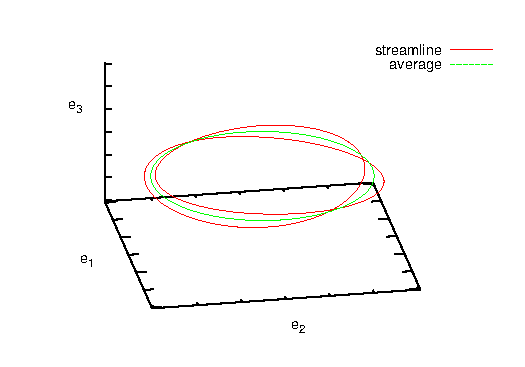
\includegraphics{trefoil_knot.pdf}
%  \caption{
%    A possible streamline (red) with its averaged rotation in green.
%    The streamline was chosen to be a trefoil knot. The reasons for the non-trivial topology are discussed in the text.
%    }
%    \label{fig:particle}
% \end{figure}

\subsection{Interactions between spinless charges}\label{sec:spinless}
When an acoustic charge has no spin (or the spin is ignored)
the equations of motion can be derived from the manifestly gauge invariant energy momentum tensor in  equation \eqnref{TAEM}.
By taking the  divergence and picking out the spatial terms,
the force $\vf$ is found to be \cite{Doran2003}
\begin{align}
  \vf = - \lr{\rho_q\vE + \vJ \times \vB}.
\end{align}
If it is assumed that an acoustic charge $q$ is carried by an `acoustic particle' (a vortex tube without swirl, for instance)
moving at speed $\vu$, then
$\vf = - q\lr{\vE + \vu \times \vB}$, which is the Lorentz force law.
We argue, therefore, that turbulent sources of sound, interact according to the Lorentz-force law when measured acoustically.

Whether this result could be used to model bubble-bubble interactions remains an open question.
% The force law takes the form
% \eqal{
% \dot  u  = - \frac{q}{m_0} F \cdot u
% }{LorentzGA}
% when expressed with geometric algebra, where the dot denotes differentiation 
% with respect to proper time and $m_0$ is the {\em rest mass} of the vortex source,
% presumably the mass  displaced by the differing density of the vortex.


% The divergence of the energy momentum tensor gives the force
% and the spatial component in the lab frame is
% \begin{align}
%   \vf = - \lr{\rho_q\vE + \vJ \times \vB}.
% \end{align}
% If it is assumed that an acoustic charge $q$ is carried by a `particle' moving at speed $\vu$, then
% $\vf = - q\lr{\vE + \vu \times \vB}$, which is the Lorentz force law.
% Turbulent sources of sound, therefore, interact according to the Lorentz-force law when measured acoustically.

%\subsection{Particles with Spin}


\subsection{Other similar studies}

%The  similarities between acoustics and electromagnetism have long been recognised.
By using a relativistic version of Lighthill's formulation of aeroacoustics it was demonstrated 
that the acoustic analogue to the electric field is the Lamb vector (proportional to the Coriolis acceleration),
and that the acoustic analogue to the magnetic field is the vorticity.
%The spacetime vorticity tensor takes the role of the field tensor.
An analogy in this form has been presented before by both Marmanis\cite{Marmanis2000} and Sridhar\cite{Marmanis2000,Sridhar1998}.
However, both these attempts were constructed from Galilean fluid mechanics and so the analogy was only partial.
A complete  analogy, using a relativistic incompressible fluid, was first published by Garrido\cite{Garrido1982} long before the studies of Marmanis and Sridhar.  
Unfortunately, this article was missed by the wider community, 
and has only come to the attention of the author since completing this thesis.
%Nonetheless, the importance of the analogy to ultrasound physics is new.
%To the author's knowledge, the derivation in this report is the first time that the analogy has been  completed.
%The key step, missing in the attempts of Marmanis and Sridhar, 
%is to note that acoustics must be formulated in terms of a Lorentz invariant fluid where
%{\em the speed of sound equals the speed of light}.
%It is only when this step is made that the complete analogy exists for incompressible fluids.
%The motivation for this step is obvious only when it is appreciated that the speed of sound
%may take the role of the speed of light in a relativistic theory.



Relativistic fluids where the sound speed equals the speed of light have been studied many times before
as theoretical curiosities\cite{Taub1978,Pekeris1976, Pekeris1977}.
For example, Pekeris found that Hick's spherical vortex conserves angular momentum if and only if
the sound speed equals the speed of light\cite{Pekeris1977}.
The importance of such fluids, however, has not to the author's knowledge been recognised.
Such fluids represent {\em what can be measured} when distances are obtained by echo-location.
%Acoustics as measured with ultrasound is therefore {\em identical} to electromagnetism as measured with light.
% With hindsight this correspondence is not too surprising.
% For both acoustics as measured with ultrasound and electromagnetism as measured with light 
% attempt to measure the properties of their propagating signal.
% Both, therefore, 
% represent a similarly limited view of the world,
% the limitations manifesting themselves in the linearity of the equations.

An alternative  analogy between acoustics and special relativity is found in the `acoustic analogue gravity' literature (see Barcel{\'o}, Liberati and Visser\cite{Barcelo2005} for a review).
An {\em acoustic} metric is constructed that describes sound carried in bulk flow.
While the description of space and time in this formulation is Euclidean, the acoustic metric turns out to be pseudo-Euclidean,
and therefore obeys the Lorentz transformation.
This results because  sound carried away by a supersonic flow will never reach us
and so the speed of sound is a limiting velocity in transformations.
The analogue gravity literature then goes on to study the gravitational implications of the acoustic metric.
The acoustic metric, albeit Lorentzian, is not the same as Minkowski's metric used here, 
but is a function of the bulk flow.
Analogue gravity does not consider the measurement process and  operates within a world characterised by two metrics, 
the Lorentz invariant acoustic metric
 and the Galilean invariant spacetime  metric.
The correspondence of analogue gravity with relativity theory is therefore partial.
The acoustic analogue to special relativity presented here is complete,
the only difference is that the speed of sound takes the role of the speed of light.


%While the motivations behind the two approaches is similar, in particular the demand that acoustics must be obey a Lorentz invariant metric,
%the approach given here and the approach of analogue gravity are fundamentally different.
%Analogue gravity does not consider the measurement process and so operates within a world characterised by two metrics, 
%the Lorentz invariant acoustic metric (which is a function of the bulk flow)
% and the Galilean invariant spacetime  metric.
%This report argues that only one metric is required;
%the acoustic analogue to special relativity presented here is identical to the original, excepting that is 
%The specPhysics that is measured 
%%Ultrasound measurement demands that the world be described by a Lorentz invariant metric.
%%There is no other way to describe space and time acoustically.
%%In analogue gravity the acoustic metric is Lorentz-invariant, but is not the same as the metric used here.
%%In analogue gravity the metric is a function of the bulk flow,
%%whereas  we argue that this is impossible:
%%the sound speed must be an a priori constant in order to say anything about the world.
%Nevertheless, the success of analogue gravity is very encouraging.
%%Acoustically observed microbubbles could offer an interesting experimental model in this field.




%%% Local Variables: 
%%% mode: latex
%%% TeX-master: "../../tshorrock_thesis"
%%% End: 

%\chapter{Digression - The exact analogy between ultrasound measured acoustics and electromagnetism}\label{ch:interactions}

\newcommand{\Tgi}{T_{\textrm{gi}}}
\newcommand{\OmegaEM}{\Omega_{\textrm{EM}}}

 %\newcommand{\tm}{\tau^-}
 %\newcommand{\tp}{\tau^+}

 % \newcommand{\vx}{\vect{x}}
  \newcommand{\vf}{\vect{f}}
  \newcommand{\J}{{\cal J}}
 \newcommand{\vJ}{\vect J}
 % \newcommand{\vj}{\vect j}
  \newcommand{\vE}{\vect E}
  \newcommand{\vB}{\vect B}
 \newcommand{\vEnr}{\vect{E}_{\textrm{nr}}}
 \newcommand{\vBnr}{\vect{B}_{\textrm{nr}}}
% \newcommand{\va}{\vect a}
% \renewcommand{\vA}{\vect A}
% \newcommand{\jp}{\pi}
 \renewcommand{\M}{\alpha}
 \newcommand{\vP}{\vect P}
%\newcommand{\vf}{\vect f}
% \newcommand{\vF}{\vect F}
% \renewcommand{\AA}{\mathbbm{A}}

 \newcommand{\Dt}{D_t}
% \newcommand{\fbar}{\underline{f}}
 \newcommand{\adjoint}[1]{\bar{#1}}
% \newcommand{\fadj}{\adjoint{f}}

% \newcommand{\zitter}{zitterbewegung}
%\begin{abstract}
%An exact acoustic analogy of electromagnetism is derived
%from a relativistic, isentropic, ideal fluid where the speed of sound is 
%set equal to the speed of light.
%Sound waves and acoustic sources in such a fluid are described by Maxwell's equations.
%It is argued that this is the correct formulation of acoustics 
%when measurements are made with a sonar based technique such as ultrasound.
%\end{abstract}


\section{Introduction}

In \chapref{measurement} we argued that ultrasound is a relativistic theory,
where the sound speed takes the role of the speed of light.
This was argued in terms of the  ultrasound measurement process,
that a constant sound speed must be known before anything can be said about distance.
We also assumed  physical invariance between inertial observers
on the belief that ultrasound should not change this.

Acoustics was then formulated for  a ideal and isentropic fluid.
Consistency with the measurement process required the fluid to be relativistic, 
in the sense that is invariant to Lorentz transformations.
To enforce the sound speed to take the role of the speed of light, 
these two constants were equated.
By enforcing the conservation of the energy momentum tensor
(or equivalently, by Noether's theorem, translational invariance)
we found the temporal and spatial equations of motion,
\eqa{
  \del \cdot A  =0 \tag{\ref{eqn:eomTime}}
}
and
\begin{align}
v \cdot \lr{\del \wedge A} = 0, \tag{\ref{eqn:eomSpace}}
\end{align}
respectively,
where c.g.s. units have been  used.
%From this latter condition a to a conserved energy momentum tensor yields
%
%This latter condition yielded the equation of state $p = \epsilon$,
%where $p$ is the thermodynamic pressure and $\epsilon$ is the total energy density.
%Our starting point was the  conservation of the energy momentum tensor,
%which by Noether's theorem is equivalent to demanding translational invariance.
%
From \eqnref{eomTime} we found that it follows that sound waves and acoustic sources are described by Maxwell's relation,
\eqa{
\del F = J, \tag{\ref{eqn:Maxwell}}
}
where 
\eqa{
  F = \del \wedge A\tag{\ref{eqn:DefnVorticity}}
} is the spacetime vortiticy,
and $J$ is the acoustic source in the wave equation $\del^2 A = J$.
The potential $A \equiv 2\sqrt p v$, where $v$ is the velocity of a fluid particle.

The consequences of this correspondence were not explored, however,
and we tie this loose end here.
In \secref{int:EM} and find that 
the role of magnetism is played by the spatial vorticity of the fluid,
and that the electric field corresponds to the Coriolis acceleration.
The space-time vorticity tensor assumes the role of the electromagnetic field tensor.
This completes similar but partial  attempts by others to construct an analogy between acoustics and electromagnetism.
In particular, both Marmanis\cite{Marmanis2000} and Srihar\cite{Sridhar1998}
have suggested and analogy between vorticity and magnetism, 
and the Coriolis acceleration (or Lamb vector) with the electric field.
However, both authors constructed their analogy in the incompressible Galilean frame, 
and therefore could not write down a wave equation (Maxwell's relation).

% For dimensional consistency we find that the acoustic charge must be {\em dimensionless}.
% The analogue to the electric permittivity has dimension $\joule^{-1}\metre^{-1}$.
% We do not have a satisfactory interpretation for the permitivity, however.

% The formal exactness of the analogy presented here implies
% that the Lagrangian for acoustics (as measured with ultrasound)
% is the same form as the electromagnetic Lagrangian.
% In \secref{int:spin} this fact is used with the further assumption of rotational invariance,
% which  by Noether's theorem demands that angular momentum is conserved,
% to show that an acoustically measured sound wave -just as light- has an intrinsic spin.

The equivalence between electromagnetism and acoustics (as measured with ultrasound)
poses several issues of interpretation:
\nlist{
  \item On the one hand sound is a longitudinal wave, the molecules vibrate parallel to the  perturbation. 
    On the other hand, sound is transverse in the Coriolis acceleration and vorticity.
    In what sense are these two views consistent?
  \item Non-linear propagation is known to be important in ultrasound,
    however, in our formulation it is impossible.
    How can this be.
%  \item Rotational invariance implies that sound has an intrinsic angular momentum.
%    Since there are two possible polarisation of the  Coriolis acceleration and vorticity
%    the sound must be spin 1.
%    What does this mean in terms of the dynamics of the fluid particles?
}
Solutions to both these problems are suggested in \secref{Interpretations}.


%interpretations to these are provided in \secref{FutureWork}.
%There is a speculative nature to these interpretations, however,
%which is why they are considered as future work.
%The difficulties in interpretation come not from dought in the validity

%In \secref{int:spin} we impose rotational invariance,
% the consequences of the correspondence between electromagnetism and acoustics.
%For instance it follows immediately  that sound, when measured acoustically,
%can be considered as transverse wave with respect to  the vorticity and Coriolis acceleration.
%If we further assume of rotational invariance, 
%which by Noether's theorem demands that angular momentum is conserved,
%then we find that sound - just as light - has an intrinsic spin.


% An interpretation of the acoustic spin is provided from the helicity.
% The acoustic analogue to the electromagnetic helicity is identical to the hydrodynamic  helicity introduced by Moffatt.
% It is s a topological invariant that describes the linking between vortex rings,
% and is, therefore, quantised.
% The spin of the sound wave describes the propagation of this topological feature through the medium.

% With these results in hand we consider acoustic-vortex interactions in \secref{int:vortex_interactions},
% important when sound interacts with a region of turbulence.
% When the spin plays no role (unlinked vortices in the turbulence) 
% we find that the interactions are described
% by Lorentz force law.
% This linear relation is a very simple and elegant solution to a difficult problem.
% It also highlights the general rule that the  acoustic measurement greatly simplifies the measured physics.
% This is because acoustic measurement intrinsically limits what can be known about the world.

% The exact analogy suggests that there might be an acoustic analogue to the electron: 
% a particle with helicity that interacts with the spin of the acoustic field.
% We do not succeed in finding the analogue, 
% but a start is suggested in \secref{int:electron}.






 

%Sir James Lighthill, in his formulation of acoustics \cite{Lighthill1952},
%gave a general framework for calculating the sound generated by turbulence with a minimum of approximation.


%The influence of boundaries was added to the formulation by Curle \cite{Curle1955} and Ffowcs Williams and Hawkings \cite{FfowcsWilliams1969}.
%More recently,  formulations in terms of the vorticity and enthalpy have also proven useful \cite{Howe1998}.
%Development has been rapid, and this must be due, in no small part, to the common point of departure enabled by Lighthill.
%The relation of special cases to the whole is clear, it is easy to see the wood from the trees.
% The turbulent sources in Lighthill's theory will in general interact with each other.
% There is a long history in studying the interactions of vorticies \cite{Whittaker1951}, 
% but yet no 
% where the force between the rings `acts at a distance', and  propagates through the medium via sound waves.
% The vorticity formulation of Lighthill's equation, therefore,
% seems ideally placed to formulate sound-acoustic source dynamics in a general way.
% This is a difficult problem in general,
% but a simple solution is possible when the interaction is measured by ultrasound,
% and is outlined in \secref{Lorentz}.
% It turns out that ultrasound is simpler than acoustics in general due to the way in which ultrasound defines time and space.
% This is discussed more in \secref{Measurement}.

% In medical ultrasound, however, the interaction of purely turbulent sources of sound are not of primary interest.
% Rather, focus is directed at the  interactions between  micron-sized pulsating bubbles that are used as contrast agents.
% Usually, when modelling such interactions the fluid is linearised early \cite{Crum1974,Leighton1990, Mettin1997},
% and so any effect of vorticity and turbulence is ignored$rho.
% This is unsatisfactory for two reasons.
% \nlist{
% \item Although the pulsating bubble is likely to dominate the sound generated in a region of turbulence,
%   it does not necessarily follow that the {\em motion } of the bubble is independent of the vorticity in the surrounding fluid.
% \item By linearising the fluid the general framework for sound-acoustic source interactions is being abandoned.
% }
% The first of these problems is the greater when it comes to predicating the results of an experiment.
% However, the second is the more grave.
% By approximating too early the theory becomes separated from the general theory of sound-source interaction, and progress becomes slow.
% Indeed, the Bjerknes force law that is often used to describe the interactions of bubbles has changed little since it was written down in 1905 \cite{Bjerknes1905},
% and this is not because it is without  problems.

% In this report we attempt to bring the description of the motion of a bubble within the Lighthill framework for ultrasonics outlined in \secref{Lorentz}.
% This is attempted in \secref{Zitter}.






\section{The acoustic analogues to the electric and magnetic fields}\label{sec:int:EM}

In classical electromagnetism the electric and magnetic fields are 
3-dimensional vector fields that are measured (usually) in the laboratory frame.
Such spatial vector quantities we denote in bold.
%The laboratory frame is represented by an inertial and orthonormal frame with basis vectors $\{\gamma_\mu| \mu = 0,1,2,3\}$,
%where $\gamma_0$ is a timelike vector with positive signature ($\g^2 =1$) 
%and $\{\gamma_k | k=1,2,3\}$ are spacelike with negative signature ($\g^2=-1$).

The most direct method of obtaining the analogues  is to project the vorticity bivector, $F$, into the laboratory  frame\cite{Hestenes2003, Doran2003}.
The analogue to the electric field can then be defined to be the timelike component, and the analogue to the magnetic field the spacelike component.
The directness of this method, however, comes at the cost of it bearing little  resemblance to conventional acoustics.

To demonstrate the similarities and the differences of ultrasound formulation of acoustics  to the Gallilean formulation,
we re-derive Maxwell's relation using an argument very similar to Lighthill's acoustic analogy\cite{Lighthill1952} of aeroacoustics.
The analogues to the electric and magnetic field  become clear in this process.

We start  by projecting the temporal and spatial equations of motion, equations \eqnref{eomTime} and \eqnref{eomSpace}
into the laboratory frame.
The result is
\sub{
  \begin{align}
     \vdel \cdot \vA &=  - \dt \phi, \label{eqn:Rcontinuity}\\ % &\quad\text{and} &&
\dt \vA - \vv \times  \lr{\vdel \times \vA} \label{eqn:REuler}
&= - \vdel \phi.
  \end{align}
}
$\phi$ and $\vA$ are the temporal and spatial components of the vector potential $A$.
%\eqa{
%\phi &\equiv  \gamma \lr{c^2 + w}  \\ %= A \cdot \g,\gamma \frac{\epsilon + p}{\rho} 2\gamma  p^{1/2}
%& \quad\text{and} &&
%\vA &\equiv  \phi \vv,  %A \wedge \g.
%}
As we found in \secref{measurement:alterations}, $\phi$ may be interpreted as the total enthalpy density,
and $\vA = \phi \vv$.
$\vv$ is the three dimensional velocity.

%Equation \eqnref{continuity} is the ultrasound equiv
Equations \eqnref{Rcontinuity} and \eqnref{REuler} are the acoustically measured versions of the continuity and Euler equations.
In the non-relativistic limit the equations reduce to Galilean invariant forms, 
\sub{
\begin{align}
  \vdel\cdot\lr{\rho \vv}  &= -\dt \rho, \label{eqn:NRcontinuity}\\
  \dt \vv - \vv\times \lr{\vdel\times \vv} &= - \vdel \phi,\label{eqn:NREuler}
\end{align}
}
with 
equation \eqnref{NREuler} being Euler's equation written in Crocco's form\cite{Howe1998}.
The difference between the two sets of equations is that the mass density, $\rho$, in the Gallilean forms is
replaced by the total enthalpy density $\phi$. 
Replacing the mass with an energy is typical of Lorentz invariant theories.

With the continuity and Euler equations in hand,
we may now apply the conventional formulations of acoustics.
We proceed with Lighthill's acoustic analogy\cite{Lighthill1952, Howe1998}.

To do so we   differentiate  the continuity equation (equation \eqnref{Rcontinuity}) with respect to time 
and subtract it from the spatial derivative of  Euler's equation (equation \eqnref{REuler}).
A wave equation for the  total enthalpy results
\subl{
\eqa{
   \lr{\vdel^2 - \dt^2}\phi
  & = \vdel \cdot \lr{\vv \times\lr{\vdel \times \vA} } \equiv - \rho_q.
\label{eqn:WavePhi}
  \intertext{Next, a wave equation for $\vA$ is obtained by 
    by differentiating the continuity equation with respect to space 
    and then adding the result to the temporal derivative of Euler's equation,
    }
   \lr{\vdel^2 - \dt^2}\vA 
   &  = - \vdel\times\lr{\vdel \times \vA} - \dt \lr{ \vv \times \lr{\vdel \times \vA}} \equiv -\vJ.
    \label{eqn:WavevA}
  }
}{Waves}
In keeping with Lighthill's analogy we interpret the right hand side of \eqnref{WavePhi} and  \eqnref{WavevA} 
as an acoustic source density, $\rho_q$, and acoustic current density, $\vJ$, 
respectively.
% Notice the nice property that the current is conserved $\vdel\cdot \vJ + \dt \rho_q = 0$.

For comparison, 
had we carried out this procedure with the Gallilean continuity and Euler equation we would have obtained\cite{Howe1998},
\subl{
  \begin{align}
    \lrsquare{  \Dt \lr{\frac{1}{c^2} \Dt} - \frac{1}{\rho}\vdel \cdot \lr{\rho \vdel}}\phi &= -\frac{1}{\rho} \vdel \cdot \lr{\rho \vv \times \lr{\vdel\times \vv}} \label{eqn:WavephiREG}\\
    \lrsquare{  \Dt \lr{\frac{1}{c^2} \Dt} - \frac{1}{\rho}\vdel \cdot \lr{\rho \vdel}}\vv  &= \frac{1}{\rho} \vdel \times \lr{\rho \vdel \times \vv}. \label{eqn:WavevvREG}
  \end{align}
}{WavesREG}
These are Lighthill's equations expressed in terms of enthalpy and vorticity\cite{Howe1998}.
The operator  $\Dt = \dt + \vv \cdot \vdel$.
The left hand side of both equations \eqnref{WavesREG} describe a non-linear wave in homoentropic potential flow \cite{Howe1998}.

Equations \eqnref{WavePhi} and \eqnref{WavevA} can be simplified by introducing
\begin{align}
  \vE &= - \vv \times \lr{ \vdel \times \vA} &\text{and}&&
  \vB &= \vdel \times \vA,
\end{align}
so that
\subl{
\eqa{
   \lr{\vdel^2 - \dt^2}\phi
  & = - \vdel \cdot \vE  \equiv - \rho_q.
\label{eqn:WavePhiMax}
  \intertext{and
    }
   \lr{\vdel^2 - \dt^2}\vA 
   &  = - \vdel\times\vB + \vE \equiv -\vJ.
    \label{eqn:WavevAMax}
  }
}{WavesMax}
Equations \eqnref{WavesMax} can now be recognised as Maxwell's equations written in terms of the potentials in the Lorenz gauge\cite{Doran2003}.
The vector $\vE$ is the Coriolis acceleration, and takes the role of the electric field in the analogy.
The axial vector $\vB$ is the spatial vorticity and takes the role of the magnetic field.

Writing out Maxwell's 4 equations explicitly gives
\sub{
\eqa{
 \vdel \cdot \vE &= q,\label{eqn:M1}  \\ 
 \vdel \times \vB &= \vJ + \dt E, \label{eqn:M2}\\
 \vdel \times \vE &= -\dt\vB\label{eqn:M3},\\
 \vdel \cdot \vB &= 0\label{eqn:M4},
}
}
The acoustic interpretation of these equations are as follows:
\nlist{
\item Equation \eqnref{M1} is the definition of an acoustic source.
\item Equation \eqnref{M2} is the definition of the acoustic current.
\item Equation \eqnref{M3} is the Lorentz invariant version of the vorticity equation.
\item Equation \eqnref{M4} is an expression of Helmholtz theorem, which demands the conservation of vorticity.
}

%Equations  \eqnref{Waves} are linear, as expected.
%However, it must be emphasised that the lack of non-linearity in \eqnref{Waves} 
%is not due to approximation -  
%equations \eqnref{Waves} and \eqnref{WavesREG} are equally exact.
%Ultrasound acoustics is simpler because less can be 
%known about the medium when it is measured acoustically.

%forms,where $\rho$ is the mass
%It is worthwhile here making a direct comparison.




% The 
% so that
% \eqa{
%  F = F\g\g = \lr{F\cdot\g}\g + \lr{F\wedge \g}\g.
% }
% The analogue to the electric field, $\vE$, and magnetic field, $\vB$,
% %In keeping with convensional formulations of classical electromagnetism,
% %we define the analogues to the electric field, $\vE$, and magnetic field, $\vB$,
% can then be defined \cite{Hestenes, Doran2003} to be 
% \sub{ 
% \label{eqn:DefnEB}
% \eqa{
%   \vE &\equiv  \lr{F\cdot\g}\g = \frac{1}{2}\lr{ F- \g F \g  } = -\dt \vA - \vdel \phi\label{eqn:DefnE}\\
%   \intertext{and}
%   I\vB  &\equiv  \lr{F\wedge\g}\g =  \frac{1}{2}\lr{ F+ \g F \g } = \vdel \wedge \vA,\label{eqn:DefnB}
% }
% }
% respectively.
% Here  $\phi = 2\gamma\sqrt{p}$
% and $\vA = \phi \vv$ are the temporal and spacial components of $A$,
% $\gamma = (1-\vv^2)^{-1/2}$ is the Lorentz  factor and $\vv$ is the spatial velocity vector.
% The term $I$ in \eqnref{DefnB} represents the spacetime pseudoscalar,
% or the `unit volume element' of spacetime.

% To find the rightmost side of \eqnref{DefnE} and \eqnref{DefnB} equation \eqnref{DefnVorticity} has been used,
% and the vector identity $a \cdot \lr{d B} = a\wedge B + d a\wedge B$ for vectors $a$ and $d$, and multivector $B$, is helpful for  \eqnref{DefnB}.
% The spacetime vorticity then exhibits the same `complex' structure as the electromagnetic field tensor,
% \eqal{
% F = \vE + I\vB,
% }{FSplit}
% where the volume $I$ takes the role of the complex number%]
% \footnote{
%   Note that $I^2= \gamma_0\gamma_1\gamma_2\gamma_3 \gamma_0\gamma_1\gamma_2\gamma_3 = -1$.
%   This geometric interpretation of complex numbers is typical of geometric algebra,
%   and gives the algebra huge power\cite{imaginary_numbers_are_not_real}.
% }.

% Expressing \eqnref{DefnB} in terms of the convensional Gibbs vector cross product, denoted with a $\times$,
% we find that $\vB = -I \vdel \wedge \vA \equiv \vdel \times \vA$, 
% and so that the axial vorticity vector is the analogue to the magnetic field.

% An alternative expression for the analogue to the electric field can be found by using equation \eqnref{FSplit} 
% in the orthogonality condition for the velocity and vorticitiy (equation \eqnref{eomSpace}).
% By considering only the bivector quantities (specified by the subscript 2 on the angular brackets $\bivector{\cdot}$)
% it is found that
% \eqa{
%   \bivector{ \g v\cdot F} = \half\bivector{\g v F - \g F v} =\gamma \vE - \gamma \vv \cdot \lr{\vdel\wedge\vA} = 0.
% }
% In the calculation it is helpful to note that $I\vB$ commutes with $\g$ and $\vE$ anti-commutes with $\g$,
% as follows from the second equalities in \eqnref{DefnEB}.
% Therefore, 
% \eqa{
%   \vE = \vv \cdot \lr{\vdel \wedge \vA} \equiv - \vv \times \lr{\vdel \times \vA}, \label{eqn:E}
% }
% which is the Coriolis acceleration.
% The second identity is the result writen with the familiar Gibbs vector product.

% %To prove that the two equations \eqnref{vE1} and \eqnref{vE2} are consistent we note that
% %\eqa{
% %\vv \cdot \lr{\vdel \wedge \vA} = \vv \cdot \vdel \vA - \vdel \vv \cdot \vA = \dt \vA - 
% %}

% \subsection{Maxwell's relation in terms of the Coriolis acceleration and the vorticity}

% Taking the spacetime-split of \eqnref{Maxwell} and using
% \eqnref{FSplit}
% we obtain
% \eql{
%   \lr{\dt + \vdel} \lr{\vE + I \vB} = \rho - \vJ
% }{MaxwellSTSplit}
% where
% \eqa{
% q = J \cdot \g \quad\text{and} \quad
% \vJ  = J\wedge \g.
% }
% Separating out the respective scalar, relative vector,
% relative bivector and relative trivector parts of \eqnref{MaxwellSTSplit}  returns  four equations,
% % \eqa{
% %   \vdel \cdot \vE &= \rho,\\
% %   \dt \vE + \vdel\cdot (I\vB)  &= -\vJ,\\
% %   \del\wedge\vE + \dt(I\vB) &= 0,\\
% %   \del\wedge\vB &= 0.
% % }
% % These may be rewritten 
% \sub{
% \eqa{
%  \vdel \cdot \vE &= q,\label{eqn:M1}  \\ 
%  \vdel \wedge \vB &= I\lr{\vJ + c^2\dt E}, \label{eqn:M2}\\
%  \vdel \wedge \vE &= -\dt(I\vB),\\
%  \vdel \cdot \vB &= 0,
% }
% }
% which are Maxwell Equations written explicitly in terms of the
% acoustic fields.


\subsection{The acoustic sources}
% The acoustic
% From Maxwell's equations we may write explicit forms for the 
% acoustic sources.
% From \eqnref{M1} and \eqnref{E} we have
% \sub{
% \begin{align}
%   q = -\vdel \cdot\lr{ \vv \times \lr{\vdel \times \vA}} \label{eqn:rho}
% \end{align}
% and from equations \eqnref{M2}, \eqnref{E} and \eqnref{DefnB}  we have
% \begin{align}
% \vJ = \vdel \times \lr{\vdel\times \vA} + \dt \lr{ \vv \times \vdel \times \vA}.\label{eqn:vJ}
% \end{align}
% \label{eqn:sources}
% }
% %Note that reintroducing SI units forces the
% %analogue to the electric permittivity to be unity
% %and the analogue to the magnetic permeability to be $c^{-2}$.

% In the non-relativistic limit, equation \eqnref{rho} is 
% the turbulence source term of  Lighthill's formulation of aeroacoustics,
% when written in terms of the total enthalpy and the vorticity\cite{Howe1998}.
% Equation \eqnref{vJ}, however,  seems seldom to be used in the aeroacoustics literature.


It is interesting to note the dimensionality of the acoustic source.
To do so it is necessary to reintroduce SI units so that \eqnref{M1} and \eqnref{M2} become
\sub{
\begin{align}
  \frac{\rho_q}{\epsilon_0} = -\vdel \cdot\lr{ \vv/c \times \lr{\vdel \times \vA}} \label{eqn:rho}
%  \lrsquare{q} = \frac{\text{Energy}}{\text{distance}^2} = \frac{\text{mass}}{\text{time}^2}.
\end{align}
and 
\begin{align}
 \frac{\vJ}{c^2 \epsilon_0} = \vdel \times \lr{\vdel\times \frac{\vA}{c}} + \frac{1}{c^2}\dt \lr{ \vv \times \vdel \times \vA}.\label{eqn:vJ}
\end{align}
}
where $\epsilon_0$ is the acoustic analogue to the electric permittivity.
The units of the left hand side of \eqnref{rho} are
\begin{align}
  \lrsquare{\frac{\rho_q}{\epsilon_0}} = \frac{\text{Energy}}{\text{distance}^2}.
\end{align}
The analogue units in electromagnetism are 
\begin{align}
\lrsquare{\given { \frac{\rho_q}{\epsilon_0}}{\text{em}}} =  \frac{\text{Energy}}{\text{distance}^2\times \text{charge}}.
\end{align}
It follows that the acoustic analogue to charge is {\em dimensionless},
and the analogue to permittivity has the units 
\begin{align}
\lrsquare{\epsilon_0} = \frac{1}{\text{distance}\times\text{Energy}}.
\end{align}
We do not, however, have an adequate interpretation of the acoustic permittivity.
We suppress the issue by  returning to c.g.s. units, where $c= \epsilon_0 = 1$.


%This emphasises what is already obvious from \eqnref{rho},
%that the acoustic charge is a dynamic property of the flow.
%The unit of $\vJ$ is a source term multiplied by a velocity.
%It is consistent with  the current  being a moving charge,
%\begin{align}
%  \vJ = q \vu
%\end{align}
%with $\vu$ being the velocity of the source.

\section{The interpretation of a sound pulse}\label{sec:Interpretations}

The equivalence of the formulation of ultrasound measured acoustics and electromagnetism raises a number of issues of interpretation.
The first of these is the linearity of the theory.
Nonlinear propagation of the sound pulse is well known to be important in ultrasound physics, 
and yet it vanishes altogether in our formulation.
This issue is considered in \secref{NonlinearProp}.

The second is that a sound pulse is a longitudinal wave, the compressions and rarefactions of the density are in the direction of propagation,
whereas Maxwell's relations describe a pair of self interacting transverse waves (the Coriolis acceleration and the vorticity).
The compatibility of these two equations is discussed in \secref{transversivity}

\subsection{On the absence of non-linear propagation} \label{sec:NonlinearProp}

The linearity of the acoustic field is entirely appropriate for ultrasound.
To apply a non-linear wave equation you need to know 
the spatial variations of the speed of sound. 
%which depend in turn, upon the spatial variations of the density.
This is seen in the left hand side of equations \eqnref{WavesREG}.
As argued in \chapref{measurement}, such knowledge is impossible
when using sound to define the concept of distance:
the sound speed used by ultrasound must be a spatially invariant constant to be able to measure anything at all.
What is to be explained, therefore, 
is not why ultrasound measured acoustics is linear - this is surely correct - 
but to explain how the non-linearity found in other measurement systems  manifests itself in acoustic measurements.
To do so it is useful to frame the discussion around the linear acoustically measured equations of
\eqnref{Waves}
and their non-linear Galilean forms \eqnref{WavesREG}.

The first point to note is that the non-linearity of the Galilean formulation of sound is entirely a matter of {\em  convention}.
It would in fact be more appropriate to rewrite equations \eqnref{WavesREG} as linear wave equations with everything else interpreted as acoustic sources and currents.
Then the sound is defined as the part of an acoustic disturbance that can propagate energy away to infinity,
the rest of the disturbance being a `local' source.
This is, in fact, the usual final step of Lighthill's analogy.
The reason it is rarely performed when the analogy is written in terms of the total enthalpy and vorticity is because
the acoustic source terms become horribly complicated.
The split of source and wave in \eqnref{WavesREG} is convenient  interpretatively, but is nevertheless rather ad-hoc,
for it mixes local terms with those that can propagate indefinitely.

The influence of non-linear propagation on what can be measured acoustically is found by comparing the right hand sides of equations \eqnref{Waves} and equations \eqnref{WavesREG}.
It is seen that the only major difference between the two is the term $- \dt \lr{ \vv \times \lr{\vdel \times \vA}}$ on the right-hand-side of \eqnref{WavevA}.
This term is, if you like, the ghost of the non-linear operator $\Dt$ on what can be measured acoustically.
When measured with ultrasound it is interpreted  as part of the current.

We note that an attempt to re-incorporate the ghost  term back into some `acoustically measured non-linear operator' would be ill-conceived, 
for it would mean that the acoustic current is no longer conserved:
the term $- \dt \lr{ \vv \times \lr{\vdel \times \vA}}$ most certainly is a current.






\subsection{Interpreting the transversivity of the sound pulse} \label{sec:transversivity}


An acoustic plain wave is  a  perturbation of the fluid particles in the direction of propagation of the pulse.
It is also a transverse wave in terms of the Coriolis and vorticity fields.
We now propose a method of squaring these seemingly contradictory views.

We consider a segment of the plain wave to be a narrow tube,
so that the entire plain wave is formed by adding together many such tubes.
Within the tube a pertabation in pressure propagates the sound wave longitudinally.
Outside of the tube no such pertabation exists.

Both within and outside of the tube  there is no vorticity and so there is no propagation of the transverse wave.
On the interface of the tube, however, there is shearing of the fluid:
the molecules  within tube move as the wave passes, the molecules outside do not.
This shearing induces a {\em vortex sheet} on the interface \cite{Howe1998}.
The vorticity is confined to the sheet 
and has a strength equal to the average speed of the molecules on either side of the interface.
From the acoustic analogue Maxwell's equations, this vorticity then induces a Coriolis acceleration orthogonal to the interface.
A longitudinal wave therefore  induces a transverse wave on its boundary.

There remains a difficulty with this interpretation, however.
A transverse wave should have exactly two helicity states.
The interpretation given to the first seems, to the author at least, entirely plausible.
The second is more difficult, however.
The construction of a transverse wave with the Coriolis and vorticity vectors interchanged does not seem obvious.
Rather than speculate, 
we leave this question unanswered.



% for the direction of the vortex  difficult, however. , We have given an 
% That is, the vorticity and the 


% Within the perturbation the vorticity vanishes
% and so it is temping to state that $\vB = 0$, innihilating the helicity with it.
% However, this view is not correct.
% To see this we imagine a  wave confined to a narrow tube of radius $r$.
% The plane wave can then be constructed from many  such tubes (see \figref{tubes}).

% At the boundary of an isolated tube slipping occurs between the translating particles that carry the sound
% within the tube
% and the bulk fluid outside.
% This results in a {\em vortex-sheet}\cite{Howe} on the boundary of the tube.
% Also at the boundary there is a discontinuity in the enthalpy $\phi$, 
% carried over from the velocity contribution of $\gamma$ in \eqnref{}.
% The Corriolis acceleration, from  \eqnref{}, therefore has two components.
% A component parallel to the tube $\vE_\parallel$ from the $\dot A$ term and a perpendicular component $\vE_\perp$ from the $\vdel \phi$ term.


% which contains 
% The vorticity from adjacent tubes cancel, 
% but the vorticity at the boundary never does.
% From equation \eqnref{} (Crocco's equation, in the hydrodynamics literature)
% The vorticity on the boundary induces a Coriollis acceleration,
% we see that on the boundary the vorticity 

 
% and it is this sense that a sound pulse can be considered as a transverse Coriollis-voriticity wave.
% The transversivity must can be set in two directions which can be described as being in either a {\em left-}  or {\em right-handed polarisation state},
% and so the helicity must be in one of two states.


% Nevertheless, for the sound pulse not to have a preferred direction, 
% and therefore to conserve angular momentum,
% it is required that it the particle  streamlines form a knot over this infinite interval.
% Perhaps the simplest vortex  knot that may be considered is the trefoil knot illustrated in \figref{}.
% Topologically the trefoil knot is equivalent to two linked rings,
% each  with the same circulation, $\kappa$, as the knot.
% The helicity of the trefoil knot is accordingly $\pm2\kappa^2$.


% The helicity of a photon is $\pm\hbar$.
% If sound is knotted with the simple trefoil knot then the {\em acoustic Plank's constant} would be
% \begin{align}
%   \hbar = 2\kappa^2,
% \end{align}
% (divided by a unit momentum, see footnote \ref{footnote:dimensionallity_footnote}).

% Why $\hbar$ and therefore $\kappa$


% Moffatt's topological interpretation of helicity has been used before to  interpret the quantisation
% of the spin in electrodynamics.
% See, for example the extensive investigations into the {\em magnetic helicity} of Trueba and Ra{\~n}ada\cite{Trueba1996, Trueba2000, Ranada2002}
% (The magnetic helicity is equation \eqnref{Helicity} where the $\vA$ and $\vB$ have there electromagnetic interpretation).
% %This in fact continues the very old notion of the vortex atom
% %that goes back to the very formulation of electrodynamics.
% What is new
% in this thesis is the equivalence of electromagnetic field and the acoustical field.
% The hydrodynamic helicity is the {\em same} as the acoustic helicity;
% the  sound pulse has a quantised spin
% and  this spin may be interpreted, via the  helicity,
% as the orbital angular momentum of  the fluid particles about their mean flow.
% %\cite{Moffatt1969, Moffatt1988, Chechkin1993,  Trueba1996, Trueba2000}.

\section{Discussion}

This  chapter has explicitly formulated the (exact) analogy between ultrasound measured acoustics 
and electromagnetism.
This ties the loose ends of \chapref{measurement}, where the analogy was noticed but not explored.
It has been found that the acoustic analogue to the electric field is the Coriolis acceleration,
and that the acoustic analogue to the magnetic field is the vorticity,
The spacetime vorticity bivector takes the role of the field tensor.
The analogy in this form has long been suspected\cite{Marmanis2000,Sridhar1998},
however, to the authors knowledge this is the first time that the analogy has been  completed.
The key step, missing in previous attempts, 
is to note that acoustics must be formulated in terms of a Lorentz invariant fluid where
{\em the speed of sound equals the speed of light}.
It is only when this step is made that the analogy exists.

Relativistic fluids where the sound speed equals the speed of light have been studied many times before
as theoretical curiosities\cite{Taub1978,Pekeris1977}.
For example, Pekeris observed that Hick's spherical vortex conserves angular momentum if and only if
the sound speed equals the speed of light\cite{Pekeris1977}.
The importance of such fluids, however, has not to the authors knowledge been recognised.
Such fluids represent {\em what can be measured} when distances are obtained by echo-location.
Acoustics as measured with ultrasound is therefore {\em identical} to electromagnetism (as measured with light).
Retrospectively this correspondence is not too surprising.
For both acoustics as measured with ultrasound and electromagnetism as measured with light 
attempt to measure the properties of their propagating signal.
Both, therefore, 
represent a similarly limited view of the world,
the limitations manifesting themselves in the linearity of the equations.

Another interesting analogy between acoustics and electromagnetism is `acoustic analogue gravity' literature (see Barcel{\'o}, Liberati and Visser\cite{Barcelo2005} for a review).
The approach constructs an {\em acoustic} metric that describes the acoustics of sound carried in bulk flow.
While the description of space and time in this formulation is Euclidean, the acoustic metric turns out to be pseudo-Euclidean,
and therefore obeys the Lorentz transformation.
This results because sound carried away in bulk flow  faster than the speed of sound will never reach us.
The speed of sound is  therefore a limiting velocity in transformations.
The analogue gravity literature then goes on to study the gravitational implications of the acoustic metric.

While the motivations behind the two approaches is similar, in particular the demand that acoustics must be obey a Lorentz invariant metric,
the approach given here and the approach of analogue gravity are fundamentally different.
Analogue gravity does not consider the measurement process and so operates within a world characterised by two metrics, 
the Lorentz invariant acoustic metric and the Galilean invariant spacetime  metric.
Ultrasound measurement demands that the world be described by a Lorentz invariant metric.
There is no other way to describe space and time acoustically.
In analogue gravity the acoustic metric is Lorentz-invariant, but is not the same as the metric used here.
In analogue gravity the metric is a function of the bulk flow,
whereas  we argue that this is impossible:
the sound speed must be an a priori constant in order to say anything about the world.
Nevertheless, the success of analogue gravity is very encouraging.
Acoustically observed microbubbles could offer an interesting experimental model in this field.



% The speed of sound is similarly limiting.
% This observation is then used to pursue the 
% The approach  starts by noting that sound carried away by a bulk flow travelling faster than the speed of sound will never reach us.
% In this sense, the acoustic source is silent, and not, perhaps dissimilar to an a
% emitted by an acoustic source that is carried away by bulk flow faster than the speed of sound.Starting from the observation that it is impossible to measure the acoustics of a 

\subsection{The acoustic Lagrangian}\label{sec:int:spin}
Finally, let us use the acoustic analogy to set out some directions for future work.
%%
%
%Usually, when imagining the average motion of particles in a sound wave,
%we think of the particles oscillating back and forth as the pressure perturbation passes through.
%This is because we think of sound waves as being longitudinal.
%In equation \eqnref{Maxwell} we have an exact analogy between electromagnetism and ultrasound measured acoustics.
%that a sound waves can be considered to be a self-inducing vorticity-Coriolis wave.
%The transverse nature (with respect to the direction of propagation)  of electromagnetic waves is well known, and applies equally to the vorticity and Coriolis fields here.
%In this section we consider the implications of this observation.
%\subsection{The acoustic Lagrangian}\label{sec:lagrangian}
%From equations \eqnref{Maxwell} acoustic sources are described by the same equations that characterise electromagnetic sources.
The common mathematical  description between acoustics and electromagnetism can be enforced by deriving both from a Lagrangian of the same form.
The electromagnetic Lagrangian density is\cite{Lasenby1993, Doran2003},
\begin{align}
 \L = \frac{1}{2} F \cdot F  - A \cdot J, \label{eqn:Lagrangian}
\end{align}
and the acoustic Lagrangian is same so long as the symbols $F$, $A$ and $J$ take their 
acoustical meaning.
Note that the acoustical Lagrangian is not the same as the Lagrangian of the ideal fluid.
It describes directly the sound and the acoustic sources,
rather than the fundamental motions of the fluid particles.



%\subsection{Symmetries from the Lagrangian density}
The symmetries of \eqnref{Lagrangian} can be found by minimising the action,
\begin{align}
  S =  \int \abs{d^4x} \L(A, \del\wedge A; x).
\end{align}
In the absence of acoustic sources ($J=0$) this results in the Euler-Lagrange equation 
\begin{align}
  \d_A \L + \del \cdot  \lr{\del_{\del\wedge A}\L} = 0. \label{eqn:EL}
\end{align}
Demanding translational invariance of the action and assuming that the
Euler-Lagrange equations are satisfied results (via Noether's theorem) in the conservation of the acoustic energy momentum tensor\cite{Lasenby1993,Doran2003}  
\eqa{
   T\lr{a} = -\half F a F.
} 
Demanding rotational invariance and applying \eqnref{EL} results in the conservation of the angular momentum.
The adjoint to the angular momentum tensor is the most useful and is\cite{Lasenby1993,Doran2003}  
\begin{align}
 \adjoint{\J}(n) = A \wedge \lr{F\cdot n} +  \adjoint{T}(n) \wedge x.
\end{align}
The second term,  $\adjoint{T}(n) \wedge x$, is the orbital angular momentum of the sound pulse as
moves through space.
The first,
\begin{align}
S(n) = A \wedge \lr{F\cdot n},
\end{align}
is the intrinsic spin of the  acoustic field.

The acoustic energy momentum tensor can be applied immediately to derive the 
 force law for an acoustic source when in the presence of an external vorticity or Coriolis field.
Remembering Maxwell's relation, $\del\cdot F = J$ (equation \eqnref{Maxwell})
we obtain 
\begin{align}
 f = \scope T(\scope \del) = -\half \lr{\scope F\scope \del F + F \del F} = -\half \lr{-JF +FJ} = J \cdot F.
\end{align}
If the acoustic source has a constant rest mass, $m_0$, and moves at a speed $u$,
then, by writing  $J = q u$, where $q$ is the acoustic source, we obtain
\begin{align}
  f = m_0 \dot u = q u \cdot F, \label{eqn:LFL}
\end{align}
Equation \eqnref{LFL}  is the Lorentz force law.

To write equation \eqnref{LFL} in its more conventional form we project into the laboratory frame,
\begin{align}
J\cdot F  = \scalar{\lr{\rho + \vJ} \g\lr{\vE+I\vB}} = -\lr{J\cdot E + q \vE + q \vu\times\vB }\g.
\end{align}
The timelike $q\vu\cdot\vE $ is the work done.
The remaining spatial component is
\begin{align}
   \vf = -q \lr{\vE + \vu \times \vB},
\end{align}
which is the Lorentz force law in its usual form.

Equation \eqnref{LFL} describes how a turbulent source moves 
in the presence of external flows when measured with ultrasound.
It is an incredibly powerful result.
Its use, however, requires individual acoustic sources to be tracked though space.
This is generally beyond the capability of ultrasound,
although this is changing with the increasing availability of 3 dimensional probes.

%Its linearity is an example of the general rule that the world appears more simple
%when it is measured acoustically.
%This is because, due to the limitations on what ultrasound can measure, reassigns the temporal and spatial locations of entities so that 
%the non-linearity in their motion vanishes.

\subsection{Helicity and Spin}

The existence of the intrinsic acoustic spin raises further interpretative issues.
In the absence of satisfactory explanation for these, however, we resist the temptation to speculate.
All we say on the matter is to note that helicity of the sound wave, 
the projection of the spin on the direction of the momentum, 
is identical to the hydro dynamical helicity introduced by Moffatt\cite{Moffatt1969}.
This is interesting because the integral of the hydrodynamic helicity is a topological invariant that measures the degree of knottedness of the flow\cite{Moffatt1969}.

To see this, we introduce the helicity,
\begin{align}
  \H \equiv   \hat \vP \cdot S(\gamma_0) = \hat \vP \cdot \lr{\phi \vE - \vA \times\vE} =  \frac{\abs{\vE}^2}{\abs{\vE\times\vB}}\vA \cdot \vB.
\end{align}
where  $\hat \vP$ is the unit  Poynting vector, 
\begin{align}
 \hat\vP =\frac{\vE \times \vB}{\abs{\vE\times\vB}}.
\end{align}
and $S(\gamma_0)$ is the timelike component of the Spin 
as measured in the laboratory frame,
\begin{align}
 S(\gamma_0) % &=  A \wedge(F\cdot)  \\
 &= \half\bivector{A\g \g \lr{F\g - \g F}}\\
 &= \phi\vE - \vA \times \vE.
\end{align}
For a sound wave
%\begin{align}
$\abs {\vE} = c\abs{\vB}$
%\end{align}
and so the helicity simplifies to
\begin{align}
  \label{eqn:Helicity}
\H = \vA \cdot \vB.
\end{align}

% To interpret the spin it is useful to project it onto the direction of motion,
% yielding a scalar known as the helicity,
% \begin{align}
%   \H = \hat \vP \cdot S(\gamma_0),
% \end{align}
% where  $\hat \vP$ is the unit  Poynting vector, 
% \begin{align}
%  \hat\vP =\frac{\vE \times \vB}{\abs{\vE\times\vB}}.
% \end{align}
% and $S(\gamma_0)$ is the timelike component of the Spin 
% as measured in the laboratory frame,
% \begin{align}
%  S(\gamma_0) % &=  A \wedge(F\cdot)  \\
%  &= \half\bivector{A\g \g \lr{F\g - \g F}}\\
%  &= \phi\vE - \vA \times \vE.
% \end{align}
% The helicity is therefore
% \begin{align}
%   \H =  \hat \vP \cdot \lr{\phi \vE - \vA \times\vE} =  \frac{\abs{\vE}^2}{\abs{\vE\times\vB}}\vA \cdot \vB.
% \end{align}
% For a sound wave
% %\begin{align}
% $\abs {\vE} = c\abs{\vB}$
% %\end{align}
% and so the helicity simplifies to
% \begin{align}
%   \label{eqn:Helicity}
% \H = \vA \cdot \vB.
% \end{align}
% While $\H$ in \eqnref{Helicity} is defined in terms of the spin,
%  the 
 The term $\vA \cdot \vB$ on the right hand side is the same as the 
relativistic generalisation\footnote{ \label{footnote:dimensionallity_footnote}
The relativistic generalisation is accomplished by replacing $\vv$ in Moffatt's definition with $\vA$.
Notice, furthermore, that Moffatt did not normalise the Helicity,
that is $\H_{\text{Moffatt}} = p\cdot S$ rather than $\frac{1}{\abs{p}}p\cdot S$,
where $p$ is the momentum.
When we make the comparison to $\H = \epsilon_0 A\cdot B$, therefore,
we implicitly divide $\H_{\text{Moffatt}}$ by a unit momentum,
so that dimensionally all is correct.
} to the
{\em hydrodynamic helicity} per unit volume defined by Moffatt\cite{Moffatt1969}.
It is also  readily interpretable.
$\vB = \vdel \times \vA$ measures a rotation,
and the rotation is projected about  $\vA$.
The helicity therefore measures the degree to which the fluid streamlines rotate about themselves,
that is, the degree to which the streamlines are helical\cite{Moffatt1969, Ranada1992}.
%In a small volume $dV$ the flow is comprised of a superposition of a uniform flow $A_0$, a shear
%and a rigid body rotation about the origin of $dV$ with an angular velocity of twice the vorticity $2\vB_0$
%The streamlines of the flow within the sound pulse will be helices about the sheared $A_0$
The contribution to $\vA \cdot \vB dV \approx \vA_0\cdot \vB_0 dV$
is positive or negative depending on the orientation of the helix\cite{Moffatt1969}.

In this way Moffatt identifies the component of the spin parallel to the momentum
with the {\em orbital angular momentum} of a fluid streamline about its mean trajectory.
The equivalence between the two helicities (acoustic and hydrodynamic)
suggests that this interpretation of the spin is valid.

Finally we note that the hydrodynamic helicity was introduced by Moffatt because 
\begin{align}
  I = \int \abs{dV} \H = \int \abs{dV} \vA \cdot \vB
\end{align}
is an invariant that defines the degree of knottness of the fluid.
In the case of two vortex rings, for example, $\H =2 \alpha \kappa_1 \kappa_2$ 
where $\kappa_i$ are the circulations around the two rings. % $C_i$ of the two vortex filaments,
%\begin{align}
%  \kappa_i = \oint_{C_i} \vu \cdot d\vect{l},
%\end{align}
%where $\vu$ is the velocity around $C_i$,
%and $\alpha$ is an integer that defines the linking of the two filaments.
If they are unlinked $\alpha = 0$, whereas if they are singularly linked $\alpha = \pm 1$.
The helicity in a volume, the component of the spin parallel to the momentum, is therefore quantised
in accordance with the topology of the streamlines.

The author does not have an interpretation for this fascinating result and so does not comment further.
We note, however, that there has been considerable effort in applying the hydrodynamic helicity electromagnetism,
with implications to both the quantisation of the spin and to the quantisation of the charge.
We refer the interested reader to the literature\cite{Trueba1996, Trueba2000, Ranada2002}.




% that the projection of the spin along the direction of the acoustic momentum,
% We do not wish the resThis is necessary to avoid confusing the results already given 

% in the absence of sources ($J= 0$) by writing $A \rightarrow A + \epsilon \AA$,
% where $A$ is the  minimum field, $\epsilon$ is a small number and $\AA$ is a perturbation about $A$.
% Then 
% \begin{align}
% \frac{d S }{d\epsilon}&= \int \abs{d^4x}\lr{\AA \cdot \d_A \L + (\del\wedge \AA) \cdot \del_{\del\wedge A}\L}\\
% &= \int \abs{d^4x} \int \abs{d^4x} \AA \cdot\lr{ \d_A \L + \del \cdot  \lr{\del_{\del\wedge A}\L} } + \text{b.c}
% \end{align}
% where $\text{b.c}$ indicates the presence of  a total divergence which is assumed to vanish on the boundary.
% When $S$ is minimised,
% \begin{align}
%   \d_A \L + \del \cdot  \lr{\del_{\del\wedge A}\L} = 0, \label{eqn:EL}
% \end{align}
% which is the Euler-Lagrange equation for the acoustic field.
% x\subsubsection{Transformations}
% A transformation in the underlying space 
% \begin{align}
% x \rightarrow x^\prime = f(x)
% \end{align}
% maps one location $x$ in space to another, $\xp$.
% A tangent vector $a(x)$ to the space at $x$ 
% is then mapped to 
% \begin{align}
%    a(x^\prime) = a\cdot \del f(x) \equiv \fbar(a).
% \end{align}
% The adjoint, $\fadj$ to this transformation is defined by the relation
% \begin{align}
%    b^\prime \cdot \fbar(a) = a\cdot \fadj(b^\prime) 
% \end{align}
% so that 
% \begin{align}
% \fadj(b) = \del_a  \fbar(a)\cdot b  = \del f(x) \cdot b.
% \end{align}
% It follows that
% \begin{align}
%   \del a(\xp) &= \del_b b\cdot \del a(f(x))\\
%   %&= \del_b \lr{b\cdot \del f(x)} \cdot \del_{x^\prime} a(x^\prime) \\
%   &= \del_b \fbar(b) \cdot \del_{\xp} a(\xp)\\
%   &= \fadj(\del_\xp) a(\xp).
% \end{align}
% Therefore 
% \begin{align}
%   \del &= \fadj(\del_{x^\prime}) \equiv \fadj(\del^\prime). \label{eqn:delTransformation}
% \end{align}
% All vectors must transform the same way,
% and so more generally we define
% \begin{align}
%   a^\prime(x) = \fadj(a(x^\prime)) = \fadj\fbar(a(x)).
% \end{align}

% % In summary, therefore, the transformation $\xp =  f(x)$
% % induces the transformations
% % \sub{
% % \begin{align}
% %   a(x^\prime) &=  \fbar(a(x)) 
% % \intertext{and }
% %   \del &= \fadj(\del_{x^\prime}) \equiv \fadj(\del^\prime).
% % \end{align}
% % \label{eqn:InducedTransformations}
% % }
% The action transforms under a change of coordinates as 
% \begin{align}
%   S = \int \abs{d^4x} \L(A, \del\wedge A; x) = \int \abs{d^4x^\prime}\det \fbar^{-1} \L(A^\prime, \del^\prime\wedge A^\prime; x^\prime)
% \end{align}
% and so 
% \eqa{
%   \L^\prime(A, \del\wedge A;x) = \frac{1}{\det \fbar} \L(A^\prime, \del^\prime\wedge A^\prime; x^\prime).
% }
% Parameterising the transformation by the scalar $\alpha$,  where $\alpha=0$ corresponds to the identity transformation,
% gives
% \begin{align}
% \given{\frac{d \L^\prime }{d\alpha}}{\alpha=0} &= \delta A^\prime \cdot \del_{A^\prime}\L + \lr{\del^\prime\wedge (\delta A^\prime)}\cdot \del_{\del^\prime\wedge A^\prime} \L
% \end{align}
% where the shorthand $\delta A^\prime = \frac{d A^\prime}{d\alpha}$ has been used.
% If it is assumed that  $A$ satisfies the Euler-Lagrange equation,  \eqnref{EL}, 
% then 
% \begin{align}
%   \given{\frac{d \L^\prime }{d\alpha}}{\alpha=0}  &= \del\cdot\lr{\lr{\delta A^\prime} \cdot \del_{\del^\prime\wedge A^\prime} \L}.
%   \label{eqn:dL}
% \end{align}
% %on the condition that, on the second line,  $A$ satisfies the Euler-Lagrange equation,  \eqnref{EL}.
% %If the Lagrangian density is symmetrical to the transformation the $\L$ is independent of $\alpha$ and 
% %{\em conjuagate current} $\lr{\delta A} \cdot \del_{\del_{x^\prime}\wedge A^\prime} \L$ is conserved.

% \subsection{Translational Invariance}
% If there is no priviliged position in space then the Lagrangian  density should be unchanged by the transformation
% \begin{align}
%   x^\prime = x + \alpha a,
% \end{align}
% for constant vector $a$ and scalar $\alpha$.
% The differential to the transformation is $\fbar(a) = a$
% the adjoint is  $\fadj(a^\prime) = a^\prime$,
% and the determinant is 1.
% Therefore  $A^\prime(x) = A(x)$ and the $\del = \del^\prime$.
% We also have  $\delta A^\prime = a\cdot \del A$
% and  $\frac{d \L(x^\prime }{d\alpha} = a \cdot \del \L(x)$.

% Equation \eqnref{dL} then becomes 
% \begin{align}
%   a\cdot \del \L =  \lr{a\cdot \del A} \cdot \del_F \L = \lr{a\cdot \del A} \cdot F,
% \end{align}
% from which it follows that, 
% \begin{align}
% \del\cdot\lr{\lr{a\cdot \del A} \cdot F - a\L} = 0.
% \end{align}
% The energy-momentum tensor, 
% \begin{align}
%   T(a) = \lr{a\cdot \del A} \cdot F - a\L = \lr{a\cdot \del A} \cdot F -\half a F\cdot F, \label{TEM}
% \end{align}
% is therefore conserved for translations through space-time.

% The explicit dependence on $A$ can be moved to the bounding surface\cite{Lasenby1993,Doran2003}
% by writing  $a\cdot\lr{\del \wedge A} =a \cdot \del A -  \del\lr{ A \cdot a}$
% so that
% \begin{align}
% \label{eqn:TAEM}
%   \Tgi(a) = \lr{a\cdot F}\cdot F  -\half a F\cdot F = - \half F a F
% \end{align}
% plus a total divergence, which is assumed to vanish on the boundary at infinity.
% The energy momentum tensor is then in a  manifestly gauge invariant form within the volume.
% $\Tgi$ is equal to its adjoint $\bar {\Tgi}$
% and so translational symmetry implies that  $\del \cdot \Tgi(a) = a\cdot\scope\Tgi(\scope\del) = 0$.
% This follows because
% \eqa{
%   \bar T(a) &= -\half \del_b \scalar{a F b F} \\
%   &=-\half \del_b \scalar{b F a F} \\
%   &= -\half F a F = T(a).
% }
% \subsection{Acoustic spin from rotational invariance}

% In addition to translational invariance, 
% all physical theories should be invariant to rotations:
% there should be no preferred orientation to our experiments.

% Rotations are represented by the transformation 
% \begin{align}
%   x^\prime = \Rt x R, \label{eqn:RotTrans}
% \end{align}
% where $R = e^{\alpha B/2}$ and $\Rt = e^{-\alpha B/2}$
% each represent rotations by the angle $\alpha/2$ through the plain $B$%
% \footnote{
% If $x$ is in the plain $B$ then, $B$ anti-commutes with $x$
% so that $\Rt x R = x e^{\alpha B}$. 
% Furthermore, if $B$ is composed of normal vectors of the same signature,
% for example $B = \gamma_1\wedge\gamma_2 = \gamma_1\gamma_2$ then
% $B^2= -1$.
% Equation \eqnref{RotTrans} then comprises of a rotation in the `complex plain'  $\gamma_1\gamma_2$.
% For the three spatial rotations there are three such plains and so three such complex numbers.
% These were introduced by Hamilton as $i$, $j$, $k$ in his Quaternian algebra,
% and is where, historically, the index notation comes for the three spacial axes.
% The double sided rotation of $\alpha/2$ degrees alluded Hamilton, however,
% and  this meant that rotations could only be handled if the vector to be rotated was in the same plain as the rotation.
% This made the algebra complicated, 
% and cause Gibbs to break apart Quaternian into the  $i$, $j$, $k$ axes and a scalar.
% For more on this history see the books of David Hestenes\cite{Dynamicsbook, Hestenes1984} and the Cambridge geometric algebra group\cite{Doran2003}.
% }.
% The differential of the transformation is $\fbar(a) = \Rt a R$ 
% the adjoint is $\fadj(a^\prime) = R a \Rt$ and the determinant is unity.
% Using $R\Rt =1 $ it follows that 
% \begin{align}
%   A^\prime(x) = R A(\xp) \Rt = A(x).
% \end{align}
% Using \eqnref{delTransformation} it follows that 
% \begin{align}
%  \del \wedge A = R \del^\prime \wedge A(x^\prime) \Rt = R F(\xp) \Rt.
% \end{align}
% The vector 
% \begin{align}
% \delta A^\prime &= \frac{d}{d\alpha}R A(x^\prime) \Rt \\
% &= B\cdot A + R \frac{d \xp}{d \alpha}\cdot \del A \Rt \\
% &=  B\cdot A - \lr{B \cdot x }\cdot \del A.
% \end{align}

% Using \eqnref{dL} we obtain the conserved current, the angular momentum 
% \begin{align}
%   \J(B) &= \lr{B\cdot A - \lr{B \cdot x }\cdot \del A}\cdot F+ \half B\cdot x F\cdot F\\
%   &= \lr{B\cdot A} \cdot F + T(x\cdot B)
% \end{align}
% where \eqnref{TEM} has been used.
% The adjoint is 
% \begin{align}
%   \adjoint{\J}(n) &= \del_B\scalar{\J(B) n} \\
%   &= \bivector{A F\cdot n - x\wedge \del T(x) \cdot n} \\
%   &= A \wedge \lr{F\cdot n} +  \adjoint{T}(n) \wedge x
% \end{align}
% The second term  $\adjoint{T}(n) \wedge x$ is the orbital angular momentum of the sound pulse as
% moves through space.
% The first
% \begin{align}
% S(n) = A \wedge \lr{F\cdot n}
% \end{align}
% is the intrinsic spin of the  acoustic field.
% The spin term is often suppressed by putting its influence in the boundary conditions,
% but since we are interested in acoustic plain waves we shall not do this.
% %This has the advantage of making the angular momentum manifestly gauge-invariant,
% %although at the cost of making plain-waves (that reach to infinity) more inconvenient to handle.
% %Again this isn't manifestly gauge invariant.
% %When the fields diminish rapidly at infinity the angular momentum may be  expressed in gauge invarent form,
% %the spin is absorbed into the angular momentum $T(n)$.
% %However, such a procedure is not valid for plain wave solutions (as the field does not vanish at infinity)
% % so we keep \eqnref{AM}.
% %The spin in the lab frame  is
% %\begin{align}
% %  S(v) =A \wedge   \lr{F \wedge \gamma} = -\multi{\phi + \vA \vE}_2 = \phi phi I \vB_v 
%  %  S(n) = A \cdot  \lr{F\wedge  n} =  \lr{A\cdot F} \wedge n %= -\phi I\vB
% %\end{align}
% %The spin in the lab frame  is
% %\begin{align}
% %  S(\g) =A \wedge   \lr{F \cdot \g} = -\phi \vE - I \vA \times \vE  = 
% % %  S(n) = A \cdot  \lr{F\wedge  n} =  \lr{A\cdot F} \wedge n %= -\phi I\vB
% %\end{align}

% \subsection{The acoustical spin as a quantised topological invariant}

% To interpret the spin it is useful to project it onto the direction of motion,
% yielding a scalar known as the helicity,
% \begin{align}
%   \H = \hat \vP \cdot S(\gamma_0),
% \end{align}
% where  $\hat \vP$ is the unit  Poynting vector, 
% \begin{align}
%  \hat\vP =\frac{\vE \times \vB}{\abs{\vE\times\vB}}.
% \end{align}
% and $S(\gamma_0)$ is the timelike component of the Spin 
% as measured in the laboratory frame,
% \begin{align}
%  S(\gamma_0) % &=  A \wedge(F\cdot)  \\
%  &= \half\bivector{A\g \g \lr{F\g - \g F}}\\
%  &= \phi\vE - \vA \times \vE.
% \end{align}
% The helicity is therefore
% \begin{align}
%   \H =  \hat \vP \cdot \lr{\phi \vE - \vA \times\vE} =  \frac{\abs{\vE}^2}{\abs{\vE\times\vB}}\vA \cdot \vB.
% \end{align}
% For a sound wave
% %\begin{align}
% $\abs {\vE} = c\abs{\vB}$
% %\end{align}
% and so the helicity simplifies to
% \begin{align}
%   \label{eqn:Helicity}
% \H = \vA \cdot \vB.
% \end{align}
% %On the left is the electromagnetic helicity. 
% %On the right is the acoustical helicity first defined by Moffat \cite{Moffatt1969}.

% %For the acoustic wave to be transverse in vorticity the particles being perturbed must contribute to  an angular momentum (spin) when the sound wave passes through.
% %We must therefore imagine the particles to be moving on small vortex lines, 
% %rather than `to and throw' in a linear fashion.
% %These loops must be closed, for else momentum will be passed to the fluid  after the sound wave has passed,
% %and the the longitudinal oscillation should coincide with the frequency of the wave. 
% %A motion such as the streamline in \figref{particle} could be imagined.



% %The loop drawn in \figref{particle} may seem overly complicated.
% %The reason that a simple circle, for example, 
% %would not do is due to the non-trivial topology implied by the non-vanishing helicity.
% While $\H$ in \eqnref{Helicity} is defined in terms of the spin,
%  the  term $\vA \cdot \vB$ on the right hand side is the same as the 
% relativistic generalisation\footnote{ \label{footnote:dimensionallity_footnote}
% The relativistic generalisation is accomplished by replacing $\vv$ in Moffatt's definition with $\vA$.
% Notice, furthermore, that Moffatt did not normalise the Helicity,
% that is $\H_{\text{Moffatt}} = p\cdot S$ rather than $\frac{1}{\abs{p}}p\cdot S$,
% where $p$ is the momentum.
% When we make the comparison to $\H = \epsilon_0 A\cdot B$, therefore,
% we implicitly divide $\H_{\text{Moffatt}}$ by a unit momentum,
% so that dimensionally all is correct.
% } to the
% {\em hydrodynamic helicity} per unit volume defined by Moffatt\cite{Moffatt1969}.
% It is readily interpretable.
% $\vB = \vdel \times \vA$ is measures a rotation,
% and the axis of rotation is set by $\vA$.
% The helicity therefore measures the degree to which the fluid streamlines rotate about themselves,
% that is, the degree to which the streamlines are helical\cite{Moffatt1969, Ramada1992}.
% %In a small volume $dV$ the flow is comprised of a superposition of a uniform flow $A_0$, a shear
% %and a rigid body rotation about the origin of $dV$ with an angular velocity of twice the vorticity $2\vB_0$
% %The streamlines of the flow within the sound pulse will be helices about the sheared $A_0$
% The contribution to $\vA \cdot \vB dV \approx \vA_0\cdot \vB_0 dV$
% is positive or negative depending on the orientation of the helix\cite{Moffatt1969}.

% In this way Moffatt identifies the component of the spin parallel to the momentum
% with the {\em orbital angular momentum} of a fluid streamline about its mean trajectory.
% The equivalence between the two helicities (acoustic and hydrodynamic)
% implies that this interpretation of the spin is valid.



% The hydrodynamic helicity was introduced by Moffatt because 
% \begin{align}
%   I = \int \abs{dV} \vA \cdot \vB
% \end{align}
% is an invariant that defines the degree of knottness of the fluid.
% Moffatt had a vortex rings in mind.
% For the two vortex filaments in \figref{}, for example, $\H =2 \alpha \kappa_1 \kappa_2$ 
% where $\kappa_i$ are the circulations around the two circuits $C_i$ of the two vortex filaments,
% \begin{align}
%   \kappa_i = \oint_{C_i} \vu \cdot d\vect{l},
% \end{align}
% where $\vu$ is the velocity around $C_i$,
% and $\alpha$ is an integer that defines the linking of the two filaments.
% If they are unlinked $\alpha = 0$, whereas if they are singularly linked $\alpha = \pm 1$.
% The helicity in a volume, the component of the spin parallel to the momentum, is therefore quantised
% in accordance with the topology of the streamlines.

% \subsection{Interpretation of a sound pulse}

% An acoustic plain wave is  a  perturbation of the fluid particles in the direction of propagation of the pulse.
% Within the perturbation the vorticity vanishes
% and so it is temping to state that $\vB = 0$, innihilating the helicity with it.
% However, this view is not correct.
% To see this we imagine a  wave confined to a narrow tube of radius $r$.
% The plane wave can then be constructed from many  such tubes (see \figref{tubes}).

% At the boundary of an isolated tube slipping occurs between the translating particles that carry the sound
% within the tube
% and the bulk fluid outside.
% This results in a {\em vortex-sheet}\cite{Howe} on the boundary of the tube.
% Also at the boundary there is a discontinuity in the enthalpy $\phi$, 
% carried over from the velocity contribution of $\gamma$ in \eqnref{}.
% The Corriolis acceleration, from  \eqnref{}, therefore has two components.
% A component parallel to the tube $\vE_\parallel$ from the $\dot A$ term and a perpendicular component $\vE_\perp$ from the $\vdel \phi$ term.


% which contains 
% The vorticity from adjacent tubes cancel, 
% but the vorticity at the boundary never does.
% From equation \eqnref{} (Crocco's equation, in the hydrodynamics literature)
% The vorticity on the boundary induces a Coriollis acceleration,
% we see that on the boundary the vorticity 

 
% and it is this sense that a sound pulse can be considered as a transverse Coriollis-voriticity wave.
% The transversivity must can be set in two directions which can be described as being in either a {\em left-}  or {\em right-handed polarisation state},
% and so the helicity must be in one of two states.


% Nevertheless, for the sound pulse not to have a preferred direction, 
% and therefore to conserve angular momentum,
% it is required that it the particle  streamlines form a knot over this infinite interval.
% Perhaps the simplest vortex  knot that may be considered is the trefoil knot illustrated in \figref{}.
% Topologically the trefoil knot is equivalent to two linked rings,
% each  with the same circulation, $\kappa$, as the knot.
% The helicity of the trefoil knot is accordingly $\pm2\kappa^2$.


% The helicity of a photon is $\pm\hbar$.
% If sound is knotted with the simple trefoil knot then the {\em acoustic Plank's constant} would be
% \begin{align}
%   \hbar = 2\kappa^2,
% \end{align}
% (divided by a unit momentum, see footnote \ref{footnote:dimensionallity_footnote}).

% Why $\hbar$ and therefore $\kappa$


% Moffatt's topological interpretation of helicity has been used before to  interpret the quantisation
% of the spin in electrodynamics.
% See, for example the extensive investigations into the {\em magnetic helicity} of Trueba and Ra{\~n}ada\cite{Trueba1996, Trueba2000, Ranada2002}
% (The magnetic helicity is equation \eqnref{Helicity} where the $\vA$ and $\vB$ have there electromagnetic interpretation).
% %This in fact continues the very old notion of the vortex atom
% %that goes back to the very formulation of electrodynamics.
% What is new
% in this thesis is the equivalence of electromagnetic field and the acoustical field.
% The hydrodynamic helicity is the {\em same} as the acoustic helicity;
% the  sound pulse has a quantised spin
% and  this spin may be interpreted, via the  helicity,
% as the orbital angular momentum of  the fluid particles about their mean flow.
% %\cite{Moffatt1969, Moffatt1988, Chechkin1993,  Trueba1996, Trueba2000}.




% %Moffatt demonstrated that the helicity is a measure of the degree of linking of a vortex line.
% %For a knot
% %the total helicity in a volume is an integer multiple of the number of links 
% %that exist when the  vortex line is unknotted.
% %The spin is a topological invariant, and is accordingly quantised
% %The sound field has a  quantised angular momentum, a property  not put in `by hand'.
% %We shall not persue further here the links between electromagnetism, topology and quantisation,
% %but rather refer the interseted reader to the literature 



% %Much of the interest in hydrodynamic helicity stems 
% %comes from its application to magneto-hydrodynamics.
% %Here we note a similarity between an acoustically observed fluid and a perfectly conducting fluid.
% %Both obey  $\dt \vB = \vdel \times \lr{\vv \times \vB}$,
% %which is one of Maxwell's equations in the present scheme.
% %This present discussion is but one example of what ultrasound 
% %can learn much from the magneto-hydrodynamics literature.


% % \begin{figure}[h]
% %  \centering
% %  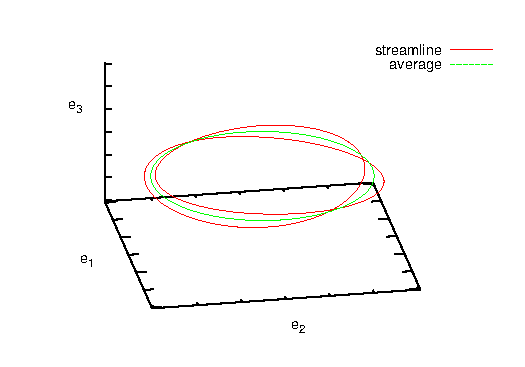
\includegraphics{trefoil_knot.pdf}
% %  \caption{
% %    A possible streamline (red) with its averaged rotation in green.
% %    The streamline was chosen to be a trefoil knot. The reasons for the non-trivial topology are discussed in the text.
% %    }
% %    \label{fig:particle}
% % \end{figure}



% \section{The force law for a turbulent  source}\label{sec:int:vortex_interaction}
% The force law for an acoustic source when in the presence of an external vorticity or Coriolis field may be found 
% from the manifestly gauge invariant energy momentum tensor\cite{Doran2003}, equation \eqnref{TAEM}.
% Remembering Maxwell's relation, $\del\cdot F = J$ (equation \eqnref{Maxwell})
% we obtain 
% \begin{align}
%  f = \scope T(\scope \del) = -\half \lr{\scope F\scope \del F + F \del F} = -\half \lr{-JF +FJ} = J \cdot F.
% \end{align}
% If the acoustic source has a constant rest mass, $m_0$ and moves at a speed $u$,
% then, by writing  $J = q u$, where $q$ is the acoustic source, we obtain
% \begin{align}
%   f = m_0 \dot u = q u \cdot F, \label{eqn:LFL}
% \end{align}
% Equation \eqnref{LFL}  is the Lorentz force law.

% To write equation \eqnref{LFL} in its more conventional form we project into the laboratory frame,
% \begin{align}
% J\cdot F  = \scalar{\lr{\rho + \vJ} \g\lr{\vE+I\vB}} = -\lr{J\cdot E + q \vE + q \vu\times\vB }\g.
% \end{align}
% The timelike $q\vu\cdot\vE $ is the work done.
% The remaining spatial component is
% \begin{align}
%    \vf = -q \lr{\vE + \vu \times \vB},
% \end{align}
% which is the Lorentz force law in its usual form.

% Equation \eqnref{LFL} describes how a turbulent source moves 
% in the presence of external flows when measured with ultrasound.
% Its linearity is an example of the general rule that the world appears more simple
% when it is measured acoustically.
% This is because, due to the limitations on what ultrasound can measure, reassigns the temporal and spatial locations of entities so that 
% the non-linearity in their motion vanishes.

% % The divergence of the energy momentum tensor gives the force
% % and the spatial component in the lab frame is
% % \begin{align}
% %   \vf = - \lr{\rho_q\vE + \vJ \times \vB}.
% % \end{align}
% % If it is assumed that an acoustic charge $q$ is carried by a `particle' moving at speed $\vu$, then
% % $\vf = - q\lr{\vE + \vu \times \vB}$, which is the Lorentz force law.
% % Turbulent sources of sound, therefore, interact according to the Lorentz-force law when measured acoustically.

% %\subsection{Particles with Spin}

% \section{Further work: Interactions between particles with spin}\label{sec:int:electron}

% The (exact) analogy developed in this thesis between acoustics and electromagnetism
% is incomplete in that we are missing an analogue to the electron:
% a particle with spin that  interacts with the spin of the sound pulse.
% We have found that turbulance is the source of the sound
% field - a role played by the electron for electromagnetic waves - 
% but we have not found an analogy of the electron itself.
% %Here we suggest path  for completing the  analogy.
% %We hope that it will  provide be a useful start to future research.

% In \secref{} we found that the spin parallel to the momentum 
% can be interpreted as resulting from  helical trajectories of the fluid particles through spacetime,
% with the spin resulting from the  orbital angular momentum of the fluid precession  about a mean trajectory.
% For this helicity not to integrate to zero,
% Moffatt demonstrated that the trajectory of the fluid particles must be knotted in some manner.
% The acoustic electron is presumably, therefore, comprised of a confined region of fluid undergoing some form of knotted helical motion.


% Interpreting the electron's trajectory as a helix about a mean trajectory is not a new idea. 
% It is at the core of the \zitter\ interpretation of quantum mechanics which dates back to Schr\"odinger.
% It has more recently overhauled by David Hestenes, and put into a form consistent with the Dirac equation\cite{}.
% In the \zitter\ interpretation the spin of the electron is interpreted as the orbital angular momentum of the electron 
% about its centre path.

% %
% %and provides the most promising starting point for our analogy.
% Using the \zitter\ as our starting point,
% we identify the electron with a region of the fluid undergoing helical motion.
% We do not assume that the actual fluid particles within the region are fixed,
% a given particle may flow through the region.
% We then use consistency with the Dirac equation to impose constraints upon this trajectory.
% As might be expected, the constraints are stringent and we are unable imagine how such a streamline can arise
% in acoustics.
% Nevertheless,
% it does give a beginning on which to build.

% \subsection{Correspondence with the \zitter\ model}

% The requirements for \zitter\ to be consistent with the Dirac equation have been catalogued.
% Here we discuss the list given in David Hestenes' article on self-interaction\cite{},
% \nlist{
%   \item the acoustic electron is a massless point particle. \label{index:massless}
%   \item the orbital-angular momentum, or spin, about the helix is fixed at $s=\hbar/2$, \label{index:spin}
%   \item the frequency of the precession is the de Broglie frequency $\omega_0 = mc^2/\hbar$,\label{index:freq}
%   \item the acoustic electron has a charge $e$
%   \item the total energy of the acoustic electron is $mc^2 = E_0 + U_0$ where $E_0$ is the kinetic energy of the helical trajectory,
%     and $U_0$ is the self-interaction potential.
% }
% From property \ref{index:massless} it follows that the helical trajectory travels at the speed of sound.
% This is not to say that the acoustic-electron travels at the speed of sound, 
% however, 
% for the projection onto the mean path will be timelike.
% From property \ref{spin} we find that the spin of the acoustic wave is constrained to be half that of the sound pulse.

% The radius of the helix is (from \ref{index:freq}) 
% \begin{align}
%   r = \frac{c}{\omega} = \frac{\hbar}{mc}
% \end{align}
% From property \ref{index:spin} it follows that
% %\begin{align}
%   $s = r\frac{E_0}{c} = \frac{\hbar}{2}$
% %\end{align}
% and so 
% \begin{align}
%   E_0 = s \omega_0 = mc^2/2
% \end{align}
% from which it follows that $E_0 = U_0 =  mc^2/2$.

% The magnetic moment - or vorticity moment - 
% is 
% \begin{align}
% \mu = \frac{ec}{2\pi r}\frac{\pi r^2}{c} = \frac{er}{2} = \frac{e}{mc}s = \frac{e\hbar}{2mc}
% \end{align}

% The Dirac current is then interpreted as the most probable mean trajectory 
% and the spin current is interpreted as the most likely direction of the spin at each spacetime point.

% \subsection{Discussion}


% To pursue the analogy between the electron and acoustics we need an algebraic system that unifies as much as possible
% classical and quantum physics.
% David Hestenes geometric algebra does this very elegantly.
% As has been forcefully demonstrated by Hestenes\cite{HestenesMechanicsBook} 
% and Doran and Lasenby\cite{Doran2003},
% much of the `quantum mathematics' has nothing intrinsically tied to quantum mechanics, 
% but rather describes mechanics in a 4-dimensional spacetime.

% Using this algebraic system
% we find that many of the features that we wish to 
% incorperate into the vortex-with-helicy-sound interaction are already present 
% in David Hestenes Zitterberegung model of the electron,
% which we use as a template.
% The  Bjerknes model of pulsations suggests an interpretation to the 
% electron's interaction parameter $\beta$, 
% which is the only parameter without adequate interpretation in the Dirac-Hestenes model.

% While the analogy between a pulsating bubble and an electron is far from satisfactory,
% it is true to say that a pulsating bubble has most of the ingredients required.
% It therefore makes an interesting first attempt, and a good point of departure for further research.





% Vortex rings with swirl,
% by virtue of their angular momentum about their symmetry axis, have been used as  classical models of spin \cite{Pekeris1953}.
% It is, however, the link between topology, helicity and spin that makes the analogy more than a useful conceptual aid.
% Moffatt \cite{Moffatt1969}, for example, when considering Hicks' spherical vortex notes  that 
% ``every torus knot is represented once and only once amongst all the vortex lines of each member of the family of flows described by the stream function''.
% Accordingly, the intrinsic angular momentum of such toroids 
% can be at least partially identified with its spin.
% %The spin will interact with an external vorticity field with a magnetic moment type reaction.
% %By appeal to the electromagnetic analogy we call the strength of the interaction the {\em magnetic moment}.
% %Since there is no danger of confusion, it seems better to use the terms of the analogy rather than introducing names such as {\em vorticity-moment}.
% %The magnetic moment is $\mu = \gamma_g \vs$ where $\vs$ is the spin vector and $\gamma_g$ is the giromagnetic ratio.
% %The energy of the interaction is $H = \mu \cdot \vB$. % and accordingly the force is $-\vdel H =-\vdel  \mu\cdot \vB$.
% %The spin-vorticity interactions need to be added
% %to the Lorentz force law of \eqnref{LorentzGA}.


% The kinematics of a vortex ring can be modelled by placing a local orthonormal coordinate frame $\{e_0, e_1, e_2, e_3\}$ at the centre of the ring.
% The vector $e_0$ is timelike and is tangent to spacetime path of the centre of the vortex, $x(\tau)$.
% Then, with $\tau$ being the proper time, $e_0 = \frac{dx}{d\tau} = u$, where $u$ is the velocity, and $e_0^2 = 1$.
% The three orthogonal axes are spacelike, so that $e_i^2 = -1,$ for $i = 1,2,3$.
% The vector $e_3 = s$ is oriented so that it is  orthogonal to the vortex ring, and is called the spin vector.
% The vectors, $e_2$ and $e_1$ define the {\em spin-plain}, $S = e_2e_1$ on which the vortex ring is confined.
% The vector $e_2$ is set to point towards the average motion of a particular swirling particle (following the green line in  \figref{particle})
% enabling the magnitude of the spin to be captured.

% %If the vortex is moving inertially, its momentum $p$ will be constant.
% %%$m$ is a measure of the vortex's intrinsic mass, perhaps the mass difference displaced by any pressure gradients within the vortex.
% %By defining and effective mass, $m =  p \cdot u$ and integrating, it follows that  $p\cdot(z - z_0) = m\tau$.
% %If the angular momentum is conserved then $lr{z - z_0} \wedge p = S(\tau) - S_0$ and so the equation of motion follows
% %\begin{align}
% %z = (S(\tau) - S_0) \cdot p^{-1} + m p^{-1} \tau + z_0 = x(\tau) + r(\tau),
% %\end{align}
% %where $x(\tau) = S_0 \cdot p^{-1} + m p^{-1} \tau + z_0 $ is the spacetime path of the central line, 
% %and $r(\tau) = S(\tau)  \cdot p^{-1}$ is the radius of the vortex ring.
% %The particle that is followed by $e_2$ is then seen to follow a helix of radius $r$ in spacetime.
% Although it is not immediately obvious,
% the model presented so far is essentially identical to the `timelike' case of the David Hestenes zitterbewegung interpretation of 
% electron physics 
% \cite{Hestenes1973, Hestenes1990,  HestenesResearchProgram}. 
% We apply the results of these papers freely, 
% although argue the results in terms of the meaning to acoustically measured turbulence. 


% The motion of the reference frame $\{e_\mu\}$ models the motion of the vortex
% and can be obtained from a constant reference frame, $\{\gamma_\mu\}$ by means a Lorentz rotation.
% Rotations are double sided transformations in geometric algebra, 
% and is written,
% $e_\mu = R \gamma_\mu \Rt$,
% where the {\em rotor} $R$ is an even multivector with reverse $\Rt$, such that $ R\Rt = 1$.
% Since geometric positioning of $\{e_\mu\}$ is all that is modelled,
% the kinematics of the frame can be completely determined by finding the
% $\tau$-dependent bivector $\Omega =  2\dot{R}\Rt $, which represents the angular
% velocity of the frame,
% %kinematics is expressed entirely by the rotor $R$,
% %such that
% %\eqal{
% %\dot{R} = \half\Omega R.
% %}{RotorEqn}
% %Alternatively, the influence on each axi
% \begin{align}
%   \dot e_\mu = \Omega \cdot e_\mu
% \end{align}
% The Lorentz force in \eqnref{LorentzGA} is of this type, with $\OmegaEM = \frac{q}{m_0}F$.
% %where $\Omega =  2\dot{R}\Rt $ is an 
% %The dynamics of the frame can be completely determined by finding the
% %$\tau$-dependent bivector $\Omega =  2\dot{R}\Rt $, which represents the angular
% %velocity of the frame.

% The energy of the fluid in the vortex is modelled by the rotation of $e_2$ in the spin plain $S$.
% Therefore, energy-momentum of the vortex is described by the rotation in this plain, $\Omega \cdot S$.
% %The quantisation of the spin in \secref{lagrangian} came from the knottedness of the flow around the spin-plain, 
% %which implies that $\oint \lr{ dx^\mu \Omega_\mu} \cdot S = nk$,
% %where $k$ is the vortex strength and $\Omega_\mu$ is the acceleration in the direction of $\gamma_\mu$.
% To include interactions with sound wave, 
% %If the vortex interacts with sound then for the angular momentum to be both conserved and obey the quantisation,
% it should be the  {\em canonical energy-momentum}, $P = p - eA$, that is equated to $\Omega \cdot S$.
% %It is appropriate that the sound contributes its energy to the spin, 
% %for this is the only way in which angular momentum is conserved. 
% Therefore
% \begin{align}
%   \Omega\cdot S = P \cdot u = m - eA\cdot v.
% \end{align}
% If a sound wave deposits $\OmegaEM \cdot S$ of energy to the vortex ring, then its mass must also increase.
% %The  $m = p \cdot u$ cannot therefore be equal to the free vortex mass $m_0$,
% %but must be
% Therefore
% \begin{align}
%   m  = p \cdot u =  \Omega \cdot S + eA\cdot v= m_0 + \OmegaEM \cdot S + eA\cdot v.
% \end{align}
% The other components of the angular velocity in the direction orthogonal to the spin plain is labelled $ v\cdot  ( I q) =- v\cdot (\Omega \wedge S)$
% while the rate at which the spin plain changes direction as it moves round its axis is $\dot S = v \cdot \del S = \Omega \times S$.
% Note that the symbol $\times$ here represents the commutator product rather than the Gibbs vector product.
% Bringing all the components together
% \begin{align}
% \label{eqn:OmegaS}
% \Omega S = \Omega \cdot S + \Omega \times S + \Omega \wedge S  = v \cdot P + \dot S + Iq
% \end{align}

% An explicit expression for $\Omega$ can be obtained by setting
% \begin{align}
%   \label{eqn:OmegaS2}
%   \Omega S &= m_0 + \OmegaEM S && \implies & \Omega &= m_0 S^{-1} + \OmegaEM = m_0 S^{-1} + \frac{e}{m_0} F.
% \end{align}
% Clearly then \eqnref{LorentzGA} is satisfied.
% Also it follows that  $\dot S = \frac{e}{m_0} F \times S$ which gives an expression for the precession of the spin plain due to the magnetic moment.

% Combining \eqnref{OmegaS} and \eqnref{OmegaS2} gives
% \begin{align}
%    v \cdot p- eA\cdot v  + v \cdot \del  S - v\cdot  (I q)=m_0 + \frac{e}{m_0} F S = m - eA\cdot v 
% \end{align}
% This is the classical approximation  of the Dirac equation in the absence of statistical terms \cite{Hestenes1990}.
% The full  equation in the absence of statistical terms is 
% \begin{align}
%  p -Iq +  = mv - \del S.
% \end{align}
% The similarities and differences  between these equations is found in the literature \cite{Hestenes1990}.


% A simple example of bound hydrodynamic helicity is Hick's spherical vortex\cite{Moffet1980}.
% This model is particularly interesting to us for it also 
% models the flow of a gas within a large bubble, where the surface tension can be neglected.
% Pulsations can futher be incorperated in an elementary way by 
% adapting the technique of Carl and Vilhelm Bjerknes to separate the interaction term caused by the pulsation 
% from the underlying force law.
% A second virtue of Hick's votex is that the angular momentum is conserved when the speed of sound is
% equal to the speed of light, which is exactly our measurement condition.
% Indeed, Pekerisis found that this conservation law applies {\em only} when the sound speed equals the speed of light.
% Pekerisis had no physical reason to impose this condition on the world, 
% but nevertheless considered the possibility of using Hick's vortex to model a neutron.
% %With the conditions of acoustic measurement considered in \chapref{measurement},
% %such a calculation seems entirely natural.
% \section{Modelling an oscillating Bubble}\label{sec:bubble}
% %Micron-sized bubbles are resonant at medical ultrasound frequencies and are used as contrast agents
% %for they  greatly enhance the signal  from blood which is generally echo-poor.
% %To consider their acoustic output it is often sufficient to ignore turbulence and simply calculate the oscillations of a monopole source.
% %However, their {\em motion} will generally not be free from turbulence effect - indeed, the microbubbles are often used to {\em measure} such turbulence.
% %It would be nice to bring their interactions with sound into the general framework presented so far.
% %To do so, the bubble is assumed to be an enclosed vortex. 
% %Toroidal bubbles bound in a region of vorticity have been observed many times - and even generated by Dolphin's in play \cite{}.
% %A spherical vortex with swirl is stable even when stationary in the fluid - and it is this flow that we imagine within a bubble.
% %In the model presented, the mass of the vortex increases when it absorbs a sound wave.
% %This models the volume fluctuations only at their most crude,
% %although for the purpose of dynamics this may be sufficient.


% To adequately model the dynamics of pulsating body such as a bubble, the  {\em interaction parameter}, $\beta$  needs to be introduced into the model.
% This can be done by substituting  $F \rightarrow F e^{I\beta}$ in the model above.
% Since the bubbles are very small, we additionally introduce a probability density $\rho$ for their location 
% - where the symbol $\rho$ should not be confused with the mass or charge density.
% Inserting these into the model above results in
% \begin{align}
%    \rho v \cdot p e^{-I\beta}  + v \cdot \del  \lr{\rho S e^{I\beta}} - \rho v\cdot  (I q)= \rho m \cos\lr{\beta}
% \end{align}
% This is the classical limit to the full Dirac equation including `statistical factors' \cite{Hestenes1973}
% The interaction intensity $\beta$ is uninterpreted in Dirac theory, although it is known to be important for determining whether an election is in a particle or anti-particle state.
% Here $\beta$ plays a similar role (it determines whether the force is attractive or repulsive).
% Whether the identification stands up to scrutiny remains to be seen.
% \section{The acoustic analogy to the electron}\label{sec:int:electron}


% %The derivation is most convenient when using David Hestenes geometric algebra\cite{} and will be used here.
% %This is because only in this algebra can Maxwell's relations be expressed in a single equation.
% %Furthermore, the vector notation of Geometric algebra should be familiar even to non-afficienardos,
% %and so its use should not be a hinderence to meaning.


% Acoustic sources will, in general, interact with one another. %, with this interaction  mediated by sound.
% %The study of vortex-vortex interactions has a  long history  \cite{Whittaker1951},
% The study of the interactions between pulsating bodies
% is of  interest in medical ultrasound because pulsating micron sized bubbles are used as contrast agents.
% The induced motion  between neighbouring bubbles has been photographed
% and the force between them is often  modelled according to Bjerknes' law  \cite{Crum1971}.
% This states that the average force on a bubble, $\scalar{f}$, is
% equal to volume displaced by the bubble, $ V$, multiplied the acceleration 
% induced by a pressure gradient, $\vdel p$ \cite{Bjerknes1905,Crum1971, Leighton1990},
% \begin{align}
%   \label{eqn:Bjerknes}
%   \scalar{f} = \scalar{V(t)\vdel p(\vx, t)}.
% \end{align}
% The  average force  over an oscillation cycle will not be zero if the bubble do not pulsate in phase with the sound wave.
% % f the oscillations arThe phase is denoted with a 
% % % and the pressure oscillates sinusoidally with a frequency $\omega$, so that  $P(\vx, t) = P(\vx)\sin\lr{\omega t}$.
% % To see that the average can give non-zero results,
% If we assume that the spatial and temporal components of the pressure may be separated, 
%  so that  $P(\vx, t) = P(\vx)\sin\lr{\omega t}$,
%  and assume that the bubble's pulsations are small, 
%  so that $V(t) = V_0\sin\lr{\omega t + \beta}$,
% then 
% $\beta$ is the phase of the bubble's oscillations in comparison to the driving sound wave.
% %Then 
% %\begin{align}
% %  \scalar{F} = V_0\vdel P(\vx) \scalar{\sin(\omega t+\beta)\sin(\omega t)} =  \frac{1}{2}V_0\vdel P(\vx) \cos(\beta)
% %\end{align}
% The resultant force over a cycle of oscillation is 
%  $\scalar{F} = \frac{1}{2}V_0\vdel P(\vx) \cos(\beta)$.
% %The strength of the force is determined by $\cos(\beta)$,
% %which can be either positive or negative.

% The  cost of this simple model is that the equations describing the surrounding fluid are linearised.
% Vorticity is not considered and we are entirely removed from the general problem of 
% turbulence-sound interaction.
% This is a shame, for while it is true that the acoustic output of a pulsating bubble far exceeds that of turbulent sources,
% turbulence is still excepted to have an influence on the bubble's motion.
% %Bubbles will not only be carried by turbulent flow but will also interact with the sound generated by it.

% Bjerknes' law, in itself, assumes little about the bubble. 
% It requires only a pulsating volume.
% The details of the bubble, such as its surface tension, are hidden in the parameter $\beta$ that specifies how close to resonance the bubble is \cite{Leighton1990}.
% The motion and interaction of a bubble, therefore, 
% can be firmly set within the context of turbulence-sound interactions, 
% so long as the bubbles mass varies when the bubble interacts with an acoustic field.
% This chimes with the attempts to use Hicks'  spherical vortex as a model of a bubble \cite{Levine1959}.
% Indeed, so long as the bubble is small compared 
% to the wavelength of the sound with which it interacts, then any vortex should do.
% %Bjerknes' law not require us to be too specific.


% In this report, as a means of investigating the interactions between bubbles and sound in its full context,
% models to describe sound-turbulence interactions in general are suggested.
% To simplify the approach we consider only the special case of when the interactions are measured acoustically,
% such as is the case when the turbulence is measured with ultrasound.
% %The formulation therefore remains general, 
% It turns out that  acoustics  is greatly simplified when imaged with sound.
% In fact,
% as is shown in \secref{measurement},
%  Lighthill's formulation of acoustics reduces to an {\em exact} analogue of electromagnetism.
% The reasons for this are briefly discussed in \secref{measurement} 
% and in more detail in a companion paper elsewhere in these proceedings.

% To find the physical consequences of the equivalence,
% the analogy is used to define an acoustic Lagrangian.
% %The exactness of the analogy has a number of consequences.
% %To find them, it is noted that since the field equations are the same, 
% %the acoustic field and the electromagnetic field 
% %can be characterised by a common Lagrangian.
% This is done in \secref{lagrangian} and the implications to angular momentum and helicity are discussed.

% Starting from the Lagrangian, the acoustic energy momentum tensor follows,
% from which the required interaction laws between sound and turbulence can be found.
% Unsurprisingly, in light of the analogy found, 
% this is the Lorentz force law  (\secref{spinless}).

% Swirl, which is  the motion along a vortex ring, for example, is harder to incorporate.
% This is because, as argued in \secref{spin}, a vortex with swirl has an intrinsic angular momentum
% which will be involved in the interaction.
% To simplify, the size of the vortex is reduced to a point.
% Its swirl and velocity can then be modelled with a co-moving frame of reference,
% %One axis of the coordinate frame traces the path of the vortex,
% %another traces the rotion.
% %The helical path through spacetime of any given particle within the vortex can then be traced.
% %This is discussed in \secref{spin}.  
% The interaction term $\beta$ is included in \secref{bubble},  enabling bubble motion to be modelled.
% The model chosen has a great deal of common with classical models of quantum  spin.
% Our thinking has been particularly influenced by David Hestenes' timelike  Zitterbegung model of the election \cite{Hestenes1973, Hestenes1990, HestenesResearchProgram}.  
% It is interesting how naturally the zitterbewegung model can be applied to turbulence.

% Finally, we note that the geometric nature of the models discussed is most straightforward
% and  concise when expressed in the {\em Spacetime Algebra} of David Hestenes \cite{Hestenes2003}.
% %This notation is sufficiently close to usual 3-dimensional vector algebra to be familiar,
% %but unfortunately space here does not permit an introduction to the algebra.
% Important results will be projected into the laboratory frame,
% so that they can be understood entirely with familiar 3-dimensional vector algebra.
% We use the convention that three dimensional vectors are displayed in bold.
% This helps to distinguish them from their spacetime analogues.

% \section{Discussion}\label{sec:discussion}

% We have constructed a general model for the dynamic interactions between sound, turbulence and bubbles.
% If the model is confirmed experimentally,
% then it represent a  relatively simple yet powerful framework in which to investigate the motion and dynamics of acoustic sources.

% In order to be able to construct the models the following observations were necessary:
% \nlist{
% \item  That the measurement process used in acoustical measurement is identical to that used in optical relativistic theories,
%     but with the speed of sound taking the role of the speed of light.
% \item  That acoustics formulated on an incompressible, relativistic ideal fluid (which embodies measurement considerations)
%     is identical to classical electromagnetism.
% }
% The authors are unaware of these observations having been made before.

% Having made the link between electromagnetism and acoustics, 
% for which a relativistic theory is  a pre-requisite,
% the application to acoustic interactions followed more-or-less mechanically.
% This indicates, on the one hand, the potential power of the analogy.
% It represents, on the other hand, a set of stringent experimental test with which to test the link between acoustics, relativity and electromagnetism.



% \section{Discussion}



% %%%%%%%%DISCUSSION
% The correspondance is exact, and successfully unifies the much observed the similarites
% between the magnetic field and vorticity (which was used by Maxwell)
% and the electric field and the corriolis acceleration (\cite{Marmanis2000,Sridar1998})
% Marmanis\cite{Marmanis} and Sridar\cite{1998} analogies were only partial 
% due to their application of the Gallilean invariance rather than
% the Lorentz invariance appropiate for electromagnetism and ultrasound.
% %%%%%%%%%%%%




% We have shown that Maxwell's equations may be derived from a relativistic (Lorentz invarient) ideal fluid,
% where the speed of sound takes the role of the speed of light.
% The Coriolis acceleration - also known as the Lamb vector - takes the role of the electric field 
% and that the vorticity takes the role of the magnetic field.
% The relativistic vorticity bivector takes the role of the field tensor.
% This identification of terms was made before by Mermanis\cite{Mermanis}.
% However, their attempt started from the Gallilean invarient approximation 
% and so Maxwell's equations could not be written down while still maintaining sound as the propergating medium.
% This work completes their analogy by making it exact.

% At first, however, the analogy derived here is dissapointing.
% A relativistic fluid, where the speed of sound equals the speed of light, 
% seems so esoteric that applications for the analogy seem in short surply.
% There is a major and terrestial application for the analogy, however,
% and that is to ultrasound physics.

% In ultrasound distances are determined from 
% \nlist{
% \item the time interval between a sound pulse leaving the transducer
% and the echo returning,   
% \item the average speed of sound of the medium.
% }
% The average speed of sound of the medium is required before anything can be said about the locations of entities
% in the world.




%%% Local Variables: 
%%% mode: latex
%%% TeX-master: "tshorrock_thesis"
%%% End: 

% LocalWords:  helicity aeroacoustics


\chapter{The pulsations of a bubble as measured with  ultrasound}\label{ch:measurement}


\section{Introduction}\label{sec:measurement:introduction}

Current models that describe the pulsations of a bubble in an acoustic field do not 
account for how measurements are made with ultrasound.
In particular, how the finiteness of the sound speed influences the spatio-temporal locations attributed to echo sources,
and limits the maximum velocities that can be measured.
Measurements made acoustically with ultrasound differ from those
made optically with a microscope due to the differing speeds of sound and light.
When a model is proposed for the pulsations of a bubble
the system of measurement that is to be used to test that model must also be specified.
%Current models have tacitly assumed that tests will be made with a microscope.
In this chapter the Keller-Miksis model 
- taken to be representative of current bubble pulsation models -
is altered to predict for the first time the pulsations that are  measured with ultrasound.

To do so it is recognised that measurements in ultrasound should be subject to the considerations of special relativity,
where the speed of sound rather than the speed of light takes the role of the limiting velocity.
This is because the pulse-echo definitions of time and space that are used in ultrasound are identical to the radar definitions used by Einstein.
Furthermore, since all ultrasound measurements are temporal,
a fixed and constant speed of sound is necessary before anything can said regarding distance.
Einstein's second postulate {\em must} be assumed for ultrasound to measure anything at all
and there is no choice but to accept the resulting discrepancies with other imaging modalities.
The only assumption made is an insistence upon invariance to inertial motions
(Einstein's first postulate).
It would be perverse for such a fundamental symmetry to be dependent on the choice of imaging modality.
%Not assuming this invariance would mark a fundamental departure for dynamics as when measured with ultrasound from
%any physics currently known.

Simulation results for the new model are presented and compared with the results from the original Keller-Miksis equation.
The acoustically-measured-Keller-Miksis equation presented here correctly predicts 
that motions of the bubble wall that exceed the speed of sound cannot be observed with ultrasound.
The radial response of the two models is similar when the harmonic response of the bubble is not strong -
otherwise the pulsations are quite different when measured acoustically and optically.


%\section{The acoustic measurement process}\label{sec:measurement:introduction}


%In medical ultrasound distances are measured using the time it takes a pulse of sound to propagate from a transducer
%to a reflecting object and then to return again. 
%%This interval is known as the pulse-echo time.
%If the sound is emitted from the transducer at a time, $\tm$,
%and the sound returns at a time,  $\tp$,
%then the task is to find from these two numbers the spatio-temporal location, $x$,
%of the point of reflection.

%What happens to the sound in between leaving the transducer and returning
%cannot be known by acoustic measurement.
%In this ignorance ultrasound practitioners assume that the time at which the echo 
%occurred is the midpoint of $\tm$ and $\tp$,
%\sub{
%\label{eqn:radar}
%\begin{align}
% \tau(x) &= \frac{\tp + \tm}{2}.
%\intertext{Other choices could certainly be made, 
%  but would imply a knowledge of the world beyond that learnt from $\tm$ and $\tp$ alone.
%  To measure distances from the times $\tm$ and $\tp$ a sound speed, $c$, is required.
%  Assuming, again in ignorance, that the sound returns at the same speed at which it left gives
%}
% \rho(x) &= \frac{\tp - \tm}{2}c. \label{eqn:radarDistance}
%\end{align}
%}
%These are the definitions of time and space that are used in ultrasound.
%%The assumption that the sound returns at the same speed as it left may be relaxed.
%%Then $\tau(x) =\epsilon \tp + (1-\epsilon)\tm$ and 
%%$\rho(x) = \epsilon \tp c - (1-\epsilon)\tm c$ for any
%%$0<\epsilon<1$.
%%This does not change any of the arguments that follow\cite{Debs1996}.

%Equation \eqnref{radarDistance} requires an {\em a priori} knowledge of the sound speed.
%This is of course obvious because ultrasound attempts to determine distances from temporal measurements.
%Nevertheless, 
%it does raise the question as to how the sound speed is to be found.

%To determine the speed of sound of a given medium an independent notion of length is required.
%This practically would be found with a set of callipers.
%The average speed of sound is then found from equation \eqnref{radarDistance},
%using the times measured and the predetermined ({\em a priori})  distance.
%The point is that %the distance measured by the callipers now represents the {\em a priori} knowledge.
%in order to use equation \eqnref{radarDistance} something must be taken for granted; 
%it is impossible to measure simultaneously both speeds and distances from temporal measurements.

%%All this is familiar. %Before ultrasound measurements can be made a calibration measurement to determine the speed of sound is required.
%%In order to use ultrasound to measure distances within people (without reaching for the callipers, and therefore for the scalpel)
%%it is necessary to first find the appropriate sound speed in the laboratory.
%%Bovine liver, typically, is used for this purpose, and is  cut into carefully measured thicknesses,
%%with care being taken to known a great deal about the sample before \eqnref{radarDistance} is applied.
%%[can you suggest a few  citations for here Jeff...]

%When using equation \eqnref{radarDistance} to measure distances the sound speed must be constant.
%This is because there is no way to measure its variations.
%This constancy of the speed of sound is identical to Einstein's  second postulate for special relativity\cite{Einstein1905},
%except that the sound speed takes the role of the speed of light.
%Likewise, Einstein used equations \eqnref{radar} for the definition of time and space, 
%except that  the  constant $c$ was understood to be the speed of light rather than the speed of sound.
%In the relativity literature equations \eqnref{radar} go by the names of radar-time 
%and radar-distance and their application to the example of the ``twin paradox'' is discussed by Dolby and Gull  \cite{Dolby2001}.

%In this thesis we  assume that the dynamics of entities is invariant to inertial motions even when measured acoustically (Einstein's first postulate).
%There has never been a counter example to this symmetry and we do not expect ultrasound to provide one.
%It then follows that measurements in ultrasound are subject to the considerations of special relativity,
%where the speed of sound rather than the speed of light takes the role of the limiting velocity.

%The surface of a  bubble that has been induced to pulsate by an ultrasound wave may collapse at a significant fraction of the speed of sound\cite{Neppiras1980}.
%The pulsations of a bubble as measured by ultrasound are therefore expected to disagree with the same pulsations measured by an optical techniques.
%To investigate this, we now derive and analyse a version of the Keller-Miksis model\cite{Keller1980} 
%- a commonly used model for a pulsating bubble - that is consistent with how ultrasound measures spatio-temporal locations.
%%This will be different than the current Keller-Miksis model that describes the pulsations of a bubble when observed optically under a microscope.


\section{The acoustically-measured Keller-Miksis model}
\subsection{The original formulation}\label{sec:KMoriginal}
The Keller-Miksis model\cite{Keller1980}  assumes that a gas bubble is located within a stationary and vorticity free fluid medium.
The fluid particles are described by the velocity potential, $\psi$.
The  bubble is assumed to remain spherical, with a  time dependent radius, $a \equiv a(t)$,
and assumed to remain at the origin.
From the spherical symmetry of the model only radial components of the velocity need to be considered. 

Keller and Miksis retain perturbations in density only up to first order, from which it follows that variations in the sound speed, $c$, are neglected
and that the velocity potential obeys the linear wave equation,
\begin{align}
\label{eqn:WaveEqn}
\lr{\dr^2 - \frac{1}{c^2}\frac{\d^2}{\d t^2}} \psi = 0.
\end{align}
The notation $\dr \equiv\frac{\d}{\d r}$ is used to denote the radial derivative
while both  $\dt \equiv \frac{\d}{\d t}$ and the over dot notation will be employed to denote the differential with respect to time.

The solution to \eqnref{WaveEqn} is
\begin{align}
  \label{eqn:Ansatz}
  \psi = \frac{1}{r}\lr{f_1\lr{t-\tfrac{r}{c}} + f_2\lr{t+\tfrac{r}{c}}},
\end{align}
where $r$ is the radial distance from the centre of the bubble
and $f_1$ and $f_2$ are functions to be determined.

Since equation \eqnref{WaveEqn} is second order two boundary conditions are required.
The first is that the radial velocity of the fluid, $v$, is equal to the velocity of the bubble wall.
That is 
\sub{
\begin{align}
  v = \dot a(t) \text{ at $r = a$.}
\end{align}
The second boundary condition is that the pressure in the liquid adjacent to the surface of bubble, $p(a,t)$,
must equal the pressure on the bubble wall, $p_b$,
\begin{align}
  p(a,t) = p_b. \label{eqn:pressureBC}
\end{align}
}
We will consider explicit expression for $p_b$ \secref{surface_pressure} and in \secref{viscosity}.

To apply these boundary conditions Keller and Miksis eliminated the spatial derivate of $\psi$ by using its definition,
\sub{
\begin{align}
  \dr \psi &= v, \label{eqn:VelocityPotNR}
\intertext{
and used Bernoulli's equation to eliminate the temporal derivatives,}
\dt \psi &= -\frac{1}{2}v^2 - h.\label{eqn:BernoulliNR}
\end{align}
}
$h$ is the enthalpy of the fluid.

The completes the specification of the model that was setup and solved by Keller and Miksis\cite{Keller1980}.

\subsection{Alterations required when making measurements with ultrasound}
\label{sec:measurement:alterations}
Equations that describe  measurements made with ultrasound require, via  special relativity,  Lorentz invariance.
Equations \eqnref{VelocityPotNR} and \eqnref{BernoulliNR} do not have this property and so 
do not apply to acoustical measurement.
To fix  \eqnref{VelocityPotNR} and \eqnref{BernoulliNR} the  relativistic generalisation to the velocity potential\cite{LandauBook} must be used,
\eqa{
  \label{eqn:RelVPot}
  \del \psi = -\frac{w u}{nc} \equiv -A.
}
Here $w$ is the heat function per proper volume and $n$ is the particle number per proper volume.
The velocity $u$ and the vector potential, $A$,  are spacetime vectors and $\del$ is the spacetime derivative.
This is the same as equation \eqnref{AisPotFlow} used in \chapref{acousticSR}. 
The heat per proper volume can be written in terms of the total energy density, 
such that\cite{LandauBook, Doran2003}
\eqa{
  w = \epsilon + p = n m c^2 + nm e + p,
}
where $e$ is the thermodynamic energy and $m$ is the proper mass.
The second equality uses equation \eqnref{relEpsilon} from \chapref{acousticSR}.
Spacetime vectors are sometimes referred to as 4-vectors, although this terminology will not be used here.
The spacetime velocity, $u$, is parameterised so that $u^2 = c^2$ where $c$ is the speed of sound.
The symbol $u$ has been used to avoid confusion with the radial component, $v$, of the spatial velocity (a 3-vector).


%
%in order for the resulting equations to be consistent with the way ultrasound assigns spatio-temporal locations to echo sources.
The temporal and spatial projections of \eqnref{RelVPot} in the laboratory frame are
\sub{
\begin{align}
\dr \psi &= \frac{\gamma w v}{nc} \equiv \frac{\phi v}{c} \label{eqn:VelocityPot}
\intertext {and}
\dt \psi &=- \frac{\gamma w  c}{n} \equiv - \phi c \label{eqn:Bernoulli}
\end{align}
}
where  $\gamma = \lr{1-v^2/c^2}^{-1/2}$ is the Lorentz factor and  the potential 
\begin{align}
  \phi \equiv \frac{\gamma w}{n} \label{eqn:phiDefn}
\end{align}
has been introduced for convenience.
The heat function per particle is related to the enthalpy by the proper mass,
\begin{align}
  w/n = \lr{mc^2 + me + p/n} = m\lr{c^2 +  h}.
\end{align}
The thermodynamic relation $h = e + p/(nm)$ has been used in the second equality.

The potential $\phi$ is the relativistic generalisation to the total enthalpy (multiplied by the proper mass).
In the non-relativistic it becomes, 
\begin{align}
  \phi \rightarrow \lr{1+\tfrac{1}{2}\tfrac{v^2}{c^2}} \lr{mc^2 + mh} = mc^2 + \tfrac{1}{2}m v^2 + mh \text{\quad as ${v/c\rightarrow 0.}$}
\end{align}
The right hand side is the energy contributed by the rest mass plus the  standard non-relativistic expression for the  total enthalpy (multiplied by the mass),
as claimed.

By replacing equations \eqnref{VelocityPotNR} and \eqnref{BernoulliNR} with equations \eqnref{VelocityPot} and \eqnref{Bernoulli} the derivation of Keller and Miksis
can be used without further alteration.
The resulting equation will be Lorentz invariant and therefore satisfy the constraints imposed by using pulse-echo to  define the spatio-temporal locations of the echo's source.


\subsection{The derivation of the acoustically-measured-Keller-Miksis equation}
Differentiating equation \eqnref{Ansatz} with respect to time obtains
\begin{align}
  r \dt \psi =  f_1^\prime + f_2^\prime, \label{eqn:dtAnsatz}
\end{align}
where the prime denotes differentiation with respect to the argument,
while differentiating with respect to the radius gives,
\begin{align}
 r^2 c \del \psi = r \lr{f_2^\prime - f_1^\prime} - c\lr{f_1+f_2}. \label{eqn:drAnsatz}
\end{align}
Equations \eqnref{dtAnsatz} and \eqnref{drAnsatz}, evaluated at $r = a$, are combined to eliminate $f_1^\prime$,
\begin{align}
  a^2 \lr{\dt \psi + c \dr \psi} - 2 a f_2^\prime + c\lr{f_1 + f_2} = 0. \label{eqn:Combo1}
\end{align}
By using equations \eqnref{VelocityPot} and \eqnref{Bernoulli} in \eqnref{Combo1} (rather than \eqnref{VelocityPotNR} and \eqnref{BernoulliNR}) 
we obtain
\begin{align}
a^2 \lr{\phi \dot a -\phi c } - 2 a f_2^\prime + c\lr{f_1 + f_2} = 0.  \label{eqn:Combo2}
\end{align}
Differentiating \eqnref{Combo2} with respect to time and reusing \eqnref{dtAnsatz} and \eqnref{Bernoulli} gives
\begin{align}
  a \frac{\phi}{c^2} \ddot a + 2 {\dot a}^2\frac{\phi}{c^2} - \phi\lr{1 + \frac{\dot a}{c}} - a \frac{\dot \phi}{c}\lr{1-\frac{\dot a}{c}} - \frac{2}{c^2} f_2^\dprime\lr{1+\frac{\dot a}{c}} = 0
  \label{eqn:Combo3}
\end{align}

The driving acoustic pressure comes from the converging acoustic wave, $f_2$.
To evaluate this term, following Keller and Miksis, 
we assume that the incident wave is planar and decompose it into  spherical harmonics.
By assumption, however, the bubble pulsates purely radially and so only the zeroth harmonic interacts with the bubble.
The potential of the incoming wave, $\psi_i (r,t)$, is accordingly 
%\begin{align}
  $\psi_i (r,t) = \frac{1}{r}\lr{f_2(t+r/c) + f_3(t-r/c)}$.
%\end{align}
Requiring that the potential is finite at the bubble's centre implies that  $f_2 = -f_3$ and so
\begin{align}
  \psi_i (r,t) = \frac{f_2(t+r/c) - f_2(t-r/c)}{r}.
\end{align}
The bubble is small in comparison to the wavelength and so the velocity potential of the fluid near the origin satisfies
\begin{align}
  \label{eqn:Tau}
 \psi_i (a,t) = \frac{f_2(t+a/c) - f_2(t-a/c)}{a} \approx \frac{2}{c}f_2^\prime(\tau).
\end{align}
The differential on the right-hand-side of \eqnref{Tau} is a function of the proper time, $\tau$, of the bubble.
This is because the equation holds only in a frame of reference where the bubble is stationary and at the origin.
Differentiating \eqnref{Tau} with respect to the proper time we obtain
\begin{align}
  \frac{d}{d \tau} \psi_i \equiv \gamma \lr{\d_t+ v\dr } \psi_i = u \cdot \del \psi = \frac{2}{c}f^\dprime.
\end{align}
Using equation \eqnref{RelVPot}  this gives
\begin{align}
\frac{2}{c}f^\dprime =-\frac{wc}{n}= - \frac{\phi_i c}{\gamma}, \label{eqn:IncidentWave}
\end{align}
where $\phi_i$ is the incident  potential.
Substituting  \eqnref{IncidentWave} into \eqnref{Combo3} and using equation \eqnref{phiDefn} in the form $\phi = \gamma m\lr{c^2 + h}$ we obtain
%\begin{align}
%  a \frac{\phi}{c^2} \ddot a + 2 {\dot a}^2\frac{\phi}{c^2} - \lr{\phi-\frac{\phi_i}{\gamma}}\lr{1 + \frac{\dot a}{c}} - a \frac{\dot \phi}{c}\lr{1-\frac{\dot a}{c}}  = 0
%  \label{eqn:Combo4}
%\end{align}
\begin{align}
  a \ddot a & \gamma \lr{1 + \frac{h}{c^2}}\lr{1 - \frac{\dot a}{c}\gamma^2\lr{1- \frac{\dot a}{c}}}+ 2 {\dot a}^2\gamma\lr{1 + \frac{h}{c^2}}\nonumber\\
  &- \lrsquare{\gamma\lr{c^2 + h} - \lr{c^2 + h_i}}\lr{1 + \frac{\dot a}{c}}- \gamma \dot h \lr{\frac{a}{c}}\lr{1 - \frac{\dot a}{c}}
= 0\label{eqn:RKM}
\end{align}
Equation \eqnref{RKM} is the final answer. The enthalpy contains the pressure terms, and with them the boundary condition of equation \eqnref{pressureBC}

 The  non-relativistic limit (with $\gamma \approx 1 - \frac{{\dot a}^2}{2c^2}$), equation \eqnref{RKM} reduces to
\begin{align}
  a \ddot a\lr{1 - \frac{\dot a}{c}}+ \frac{3}{2} {\dot a}^2\lr{1- \frac{1}{3}\frac{\dot a }{c}}
    - \lr{h - h_i}\lr{1 + \frac{\dot a}{c}}
  -  \dot h \lr{\frac{a}{c}}
= 0, \label{eqn:KM}
\end{align}
which is the original Keller-Miksis equation\cite{Hoff2001}.

The acoustically-measured-Keller-Miksis model therefore reduces to the original when the maximum speed of the bubble wall is small in comparison to the sound speed.
In the non-relativistic approximation made to obtain equation \eqnref{KM} discards terms of order $M^2$, 
where  $M = \abs{\frac{\dot a}{c}}$ is the Mach number of the bubble wall.
Therefore, the original Keller-Miksis model approximates the acoustically measured motion when $M^2$ is small.
I.e. %for acoustical measurements, the two equations may be used interchangeably 
up to about $M=0.4$.


\subsection{The applicability of the equation}
In the original derivation Keller and Miksis linearised the density. 
The consequence of this is that fluctuations in the sound speed are ignored.
This enabled our starting point, the linear wave equation of  \eqnref{WaveEqn}, to be derived.
The discarded second order terms become important when $M^2$ is not small.
The approximation holds, therefore, up to about Mach 0.4.
Interestingly,  the optical and acoustical observer
agree over the range of speeds to which the original Keller-Miksis equation is applicable.

When the measurements are made with ultrasound,
however, 
no approximation is made to obtain equation \eqnref{WaveEqn}.
The reason is that  ultrasound is not capable of  measuring variations in the speed of sound.
Second order fluctuations in the density  can therefore play no role when ultrasound is used to describe the world.
%It is instructive to see this argument borne out in the equations that describe an acoustically measured fluid.
%The equations of motion must  be Lorentz invariant and this condition  is automatically fulfilled  when  the equations 
%are obtained from the divergence of the energy-momentum tensor of the ideal fluid.
%In the derivation we also need to use the hitherto unused  condition
%that the sound speed takes the role  of the speed of light.
%This condition is imposed by equating the two speeds.
%This further requires that the energy density for the fluid, as measured acoustically, be a function of the pressure only (barotripic),
%for the sound speed cannot equal the speed of light otherwise\cite{Taub1978}.

%The energy-momentum tensor of an ideal fluid is\cite{Doran2003}
%\eqal{
%  T(a) = w a \cdot u u - a p = (\epsilon + p) a \cdot u u - a p,
%}{EMtensor}
%where, $\epsilon \equiv \epsilon(p)$ is the barotropic total energy density,
%$p$ is the pressure
%and 
%$u=u(\tau)$ is the velocity vector of the spacetime path, with the parameterisation chosen such that $u^2 = 1$. % and $P$ is the pressure.
%Natural units have been chosen in this section, and so that the speed of light is unity.

%The speed of sound, $c$,  given at constant entropy density, $\sigma$, is\cite{LandauBook,Taub1978} 
%\begin{align}
%  c^2 = \given{\frac{\d p}{\d \epsillon}}{\sigma}. \label{eqn:soundspeed}
%\end{align}
%This is the same as the non-relativistic expression except that the energy density has replaced the mass density.
%Setting the speed of sound to equal the speed of light (unity) and the integrating 
% gives,
% \begin{align}
%   \epsilon = p^\prime - p_0 + \epsilon_0
% \end{align} 
%where $p^\prime$ is a pressure that fluctuates with position, so that $dp = dp^\prime$,
%and $p_0$  and $\epsilon_0$  are the ambient  pressure and mean energy density, respectively.
%%Rather can carry the constants $ p_0 $ and $\epsilon_0$ through the rest of the derivation we write
%The thermodynamic pressure is therefore
%\begin{align}
%  p \equiv p^\prime - p_0 + \epsilon_0. \label{eqn:pshort}
%\end{align}
%and the fluid obeys the equation of state, 
%\eqal{
%  \epsilon(p) = p.
%}{eos}
%At infinity $p^\prime = p_0$ 
%and so $\epsilon_\infty = p_\infty = \epsilon_0 \ne p_0$.

%%therefore enforces that the sound speed equals that of light (unity).
%%The notation of equation \eqn{eos} is quite compact.
%%For \eqnref{eos} to be consistent with the integral of the sound speed (equation \eqnref{soundspeed}),
%%the pressure $p$ must be interpreted as follows,
%%\begin{align}
%%  p = p^\prime - p_0 + \epsilon_0. \label{eqn:pshort}
%%\end{align}
%%Here $p^\prime$ is the pressure perturbation measured with a hydrophone,
%%$p_0$  and $\epsilon_0$  are the mean  pressure and energy density respectively.



%Applying \eqnref{eos} simplifies the energy momentum tensor considerably,
%\eqal{
%  T(a) =  p\lr{2 a \cdot u u  - a} \equiv  \frac{1}{4}  A a A,
%}{EMFluid}
%where vector potential, $A$, introduced on the right hand side satisfies
%\eqal{
%  A = 2p^{1/2}u =2 \epsilon^{1/2} u.
%}{defnA}

%The vector $A$ is the same as was introduced in \eqnref{RelVPot},
%i.e.
%\begin{align}
%  \del \psi = - \frac{wu}{n} = - 2\sqrt p u.
%\end{align}
%%where $n$ is the proper particle number density of the fluid and equation \eqnref{eos} has been used for the second equality.
%To demonstrate this second equality we  use an argument of Taub\cite{Taub1978}.
%Using the isentropic thermodynamic relation $m de = - p d\lr{\frac{1}{n}}$ with the relation for the internal energy, $\epsilon= nm( 1 + e(p))$,
%it follows that 
%\begin{align}
% n d\epsilon = \epsilon dn - n^2 p d \lr{\frac{1}{n}} = \lr{\epsilon + p} dn.
%\end{align}
%Applying equation \eqnref{eos} and integrating we obtain
%\begin{align}
%  n = \sqrt p, \label{eqn:nrootp}
%\end{align}
%from which we find
%\begin{align}
%A = 2\sqrt p  u = \frac{2\epsilon}{n} u = \frac{wu}{n} =  - \del \psi,
%\end{align}
%as claimed.


%The divergence of the energy momentum tensor (equation \eqnref{EMFluid}) vanishes in the absence of external fields.
%Therefore, by projecting the divergence of \eqnref{EMFluid} along the timelike component we find
%\eqa{
%  u\cdot\scope T(\scope\del)= \half  u\cdot A \del \cdot A = 0.
%}
%The check denotes the scope of the derivative.
%Since, from \eqnref{defnA}, $A$ is parallel to $u$  it follows that 
%\eqal{
%  \del \cdot A  =0
%}{eomTime}
%and so the vector potential $A$ is conserved.
%The spacelike projection, $\scope T(\scope \del) - u u\cdot \scope T(\scope\del)$, gives in turn,
%\eqal{
%  u \cdot \lr{\del \wedge A} = 0.
%}{eomSpace}
%The relativistic vorticity bivector is 
%\eqal{F = \del \wedge A,}{DefnVorticity}
%and so \eqnref{eomSpace} implies that the vorticity is orthogonal to the velocity.

%By taking the divergence of \eqnref{eomTime} and using the vector identity
%$\del \del \cdot A = \del^2 A - \del\cdot\lr{ \del \wedge A} $
% we find,
%\eqal{
%  \del^2 A = \del \cdot F = \del F.
%}{wave}
%The second equality follows because $\del F = \del \cdot F + \del \wedge F$ 
%and because the  operator identity $\del\wedge \del = 0$ causes $\del \wedge F$ to vanish.
%Equation \eqnref{wave} is a wave equation and so interpreting the right-hand-side of \eqnref{wave} as an acoustic source current, $J$, we obtain
%\eqal{
%  \del  F = J.
%}{Maxwell}
%Interestingly equation \eqnref{Maxwell} is Maxwell's equation and equation \eqnref{eomTime} has specified that we are working in the Lorenz gauge.
%We explore this observation more in \chapref{interactions}.
%%We do not explore this observation further here.


When deriving the Keller-Miksis equation potential flow in the fluid was assumed.
This implies that the vorticity tensor vanishes, for
$F = \del \wedge A = -\del \wedge \del \psi = 0$.
Therefore the acoustic sources vanish and the wave equation $\del^2 A =0$ is satisfied.
This was the starting equation in the derivation of the Keller-Miksis model, 
equation \eqnref{WaveEqn}. 
Notice that other than potential flow, no approximation  has been made to derive \eqnref{WaveEqn}.
%When using ultrasound, sound must be measured to propagate linearly.
%This is simply because it is impossible for ultrasound to measure fluctuations in the speed of its propagating signal.
The acoustically-measured-Keller-Miksis equation is exact.

%Since no perturbation scheme has been used to obtain \eqnref{WaveEqn} when the measurements are made acoustically 
%(in contradistinction to the case when optical measurements are made)
%the acoustically-measured-Keller-Miksis equation can claim validity over a much greater range of sound speeds than the original.
%The original equation may be obtained as an approximation to the acoustically-measured-Keller-Miksis equation when the sound speed is small.
%This approximation, interestingly, is to the same order as the (quite different) approximations of the original Keller-Miksis equation.
%Therefore both acoustic measurements and optical measurements agree that the original Keller-Miksis is valid so long as $M^2$ is small.



\subsection{The pressure on the surface of the bubble}\label{sec:surface_pressure}

When introducing the original Keller-Miksis model in \secref{KMoriginal} the pressure on the surface of the bubble was not specified (equation \eqnref{pressureBC}).
In this section and the next we fix this boundary condition for the cases with and without viscosity.


The gas within the bubble may be modelled with a polytropic exponent, $\kappa$. 
The pressure within the bubble is then $p_e \lr{\frac{a}{a_e}}^{-3\kappa}$ where $p_e$ is the pressure of the gas within the bubble at equilibrium,
and $a_e$ is the radius of the bubble at equilibrium\cite{Hoff2001}.
The contribution of the vapour pressure has been neglected for simplicity.
Within the bubble pressure exceeds the pressure of the fluid at the surface, $p(a,t)$, due to the contributions of the surface tension, $\sigma$.
The pressure boundary condition is then
\begin{align}
  p_b(a) = p_e \lr{\frac{a}{a_e}}^{-3\kappa} - 2\frac{\sigma}{a}. 
\end{align}
To write the boundary condition in terms of the enthalpy we use the  thermodynamic relation $d h = \frac{1}{m n} dp$.
Substituting in $n=\frac{n_\infty}{\sqrt{p_\infty}}\sqrt{p}$, equation \eqnref{relN}, gives
\begin{align}
  h(a) =  \int_{p_\infty}^{p}  \frac{1}{m n}dp = 2\frac{\sqrt{p_\infty}}{mn_\infty}\lr{\sqrt{p}-\sqrt{ p_\infty}} = 2 \frac{p_\infty}{mn_\infty} \lr{\sqrt{p/p_\infty} - 1} 
\end{align}
%where  $n_\infty = \sqrt{p_\infty} = \sqrt{\epsilon_\infty} $ has been used in the second equality.
In the non-relativistic limit $p_\infty = \epsilon_\infty \approx n_\infty m c^2 \approx \unit{1}\giga\pascal$\cite{Hoff2001}.
This is much larger than any pressures reached in ultrasound and so we may write the pressure in terms of a fluctuations, $p^\prime$, around the ambient pressure at the surface of the bubble, $p_0$,
\begin{align}
  p = p^\prime - p_0 + p_\infty.
\end{align}
Then
\begin{align}
  h(a) =  2 \frac{p_\infty}{mn_\infty} \lr{\sqrt{1 + \frac{p^\prime - p_0}{p_\infty}} - 1} \approx \frac{p^\prime - p_0}{mn_\infty}
\end{align}
%In the non-relativistic limit $p_\infty = \epsilon_\infty \approx n_\infty m c^2 \approx \unit{1}\giga\pascal$\cite%{Hoff2001}.
%This is much larger than any pressures reached in ultrasound and so we may write, simply, that
%\begin{align}
%  h(a) \approx \frac{p - p_0}{mn_\infty}
%\end{align}


%The incident pressure $p_i$ is a perturbation about the  pressure at infinity $p_\infty$.
%Therefore
%\begin{align}
%  h_i(a) = 2\lr{\sqrt{p(a) + p_\infty }-\sqrt{ p_\infty}}.
%\end{align}

The acoustically-measured-Keller-Miksis equation is now complete. 
We emphasise that for an free polytropic gas bubble pulsating in ideal vortex-free fluid, the model is exact.


\subsection{Acoustically-measured viscosity}\label{sec:viscosity}

Viscous fluids have so far been excluded from our analysis.
Viscosity usually plays a minor role in medical applications - 
an ideal fluid does a fairly good job for modelling propagation.
However, the viscosity does play an important role in dampening the oscillations of the bubble.
In ultrasound contrast physics, therefore, the viscosity is usually incorporated into the pressure boundary condition of equation \eqnref{pressureBC}.
% Even though viscous effects have been ignored to find \eqnref{WaveEqn} they are generally incorporated into the boundary conditions.
% If they were neglected altogether there would be no dampening mechanism in the final model.
% Transient solutions to equation \eqnref{WaveEqn} would never relax and numerical studies of the resulting equations predict exotic harmonics resulting from beating between the 
% stable and transient solutions of \eqnref{WaveEqn}.
% The  second boundary condition used by Keller and Miksis is therefore
% \begin{align}
% p(a, t) =  k a^{-3\gamma} + \frac{4\mu}{3}\lr{\dr \dot a - \frac{\dot a}{a}} - 2 \frac{\sigma}{a},
%  \label{eqn:BCPressure}
% \end{align}
% }
% where $\mu$ is the viscosity and $\sigma$ is the surface tension.
To model the viscous dampening it is assumed that the fluid is Newtonian; only the  {\em  dynamic viscosity}, $\eta$, is considered. %while the {\em second viscosity} is neglected\cite{LandauBook}.
Then the stress tensor measured with ultrasound is\cite{LandauBook}, 
\begin{align}
  \sigma(a) = a p - c\eta \lr{a \cdot \del u + \del u\cdot a - a\cdot u u\cdot \del u - u u \cdot \del  u\cdot a -\tfrac{2}{3}\del \cdot u \lr{a - a\cdot u v}}.\label{eqn:RelStress}
\end{align}
The derivative with respect to the vector $a$ yields the trace\cite{Hestenes1984},
\begin{align}
  \Tr\ \sigma(a) \equiv \d_a \cdot \sigma(a) = 4p. \label{eqn:RelStressTrace} 
  % 4 p -2 c\eta \lr{ \del\cdot v  -  u\cdot \scope\del \scope v \cdot v -  \del \cdot v } = 4 p.
\end{align}
%\begin{align}
%\sigma_{00}  &=  p - \tfrac{2}{3}\eta\lr{1-\gamma^2}\lr{2\dt \gamma + 2 \vu\cdot \vdel \gamma - \gamma \vdel \cdot \vv} 
%+ 2 \eta \vv \cdot \vdel \gamma,\\
%\sigma_{ii} \equiv \gamma_i \cdot \sigma(\gamma_i) &=  -p + 2 \eta\lr{ \vdel_i \lr{\gamma \vv_i} + \gamma \vv_i/c u\cdot \del \lr{\gamma \vv_i} + \tfrac{1}{3}c\del\cdot u \lr{1+\gamma^2 %\vv_i^2/c^2 }}
%\end{align}
We wish to evaluate the radial component of the stress tensor, $\sigma_{rr} \equiv \hat r \cdot \sigma(\hat r)$, where $\hat r$ is the radial unit vector.
This is because in our spherically symmetric model it is this component that dampens the oscillation.
From \eqnref{RelStress} this is evaluated to be 
\begin{align}
  \sigma_{rr}  &= -p + 2\eta \lrsquare{\dr v + \tfrac{\gamma^2 v}{c} \tfrac{c u\cdot \del }{\gamma}\lr{\tfrac{\gamma v}{c}} - \tfrac{1}{3} c\del\cdot u\lr{1 + \tfrac{\gamma^2v^2}{c^2}}}, \label{eqn:sigmarr1}
\end{align}
where $v$ is the radial component of the velocity.
To keep the expressions short  the inner products $ u\cdot \del = \frac{\gamma }{c} \lr{\dt + v \dr}$ and $\del\cdot u = \frac{1}{c}\lr{\dt\gamma + \dr(\gamma v)}$ have not been expanded.

Equation \eqnref{sigmarr1} can be simplified by noting that $\lr{1 + \tfrac{\gamma^2v^2}{c^2}} = \lr{1 - \gamma^2\lr{1-\tfrac{v^2}{c^2}} + \gamma^2 } =  \gamma^2$.
Using a similar trick we find,
\begin{align}
   \frac{\gamma^2 v}{c} \frac{c u\cdot \del }{\gamma}\lr{\frac{\gamma v}{c}} 
=-\lr{1-\gamma^2 } \frac{c u\cdot \del }{\gamma}\gamma +\frac{\gamma^3 v}{c^2} \frac{c u\cdot \del }{\gamma}v
=\gamma c u\cdot \del \gamma. 
\end{align}
The relation $d \gamma = \frac{\gamma^3}{c^2} v d v$ has been used to obtain the second equality.
Equation \eqnref{sigmarr1} then simplifies to
\begin{align}
  \sigma_{rr}  &= -p + 2\eta \lrsquare{\dr v + \gamma c u\cdot \del\gamma - \tfrac{1}{3}\gamma^2 c\del\cdot u}. \label{eqn:sigmarr2}
\end{align}
To make further progress we re-evaluate the trace using \eqnref{sigmarr2} and the other components of the diagonal of the stress tensor,
\begin{align}
  \sigma_{tt} &= p - 2 \eta \lrsquare{\dt \gamma - \gamma c u \cdot \del \gamma - \tfrac{1}{3} \lr{1-\gamma^2} c \del\cdot u    }\\
  \sigma_{\theta\theta} =  \sigma_{\phi\phi}  &= -p + 2\eta\lrsquare{\tfrac{v}{r} - \tfrac{1}{3} c \del \cdot u},
\end{align}
and find that 
\begin{align}
  \Tr\ \sigma(a) = 4p - 2 \eta \lrsquare{2 \tfrac{v}{r} + \dr v - \dr(\gamma v) }.\label{eqn:RelStressTrace2}
\end{align}
Equating \eqnref{RelStressTrace} with \eqnref{RelStressTrace2} implies that
\begin{align}
  \dr v = - 2 \frac{v}{r}  + \dr(\gamma v)
\end{align}
and so
\begin{align}
  \sigma_{rr}  &= -p - 4\eta \lrsquare{  \frac{v}{r}  -\tfrac{1}{2}\lr{1-\tfrac{1}{3}\gamma^2}\dr(\gamma v) - \tfrac{6\gamma^2}{5c^2} v \dt v  }. \label{eqn:sigmarr3}
\end{align}

In the non-relativistic limit this equals 
\begin{align}
 \sigma_{rr}  &= -p - 4\eta \lrsquare{  \frac{v}{r}  -\tfrac{1}{3}\dr v }, \label{eqn:NRsigmarr}
\end{align}
which is  the standard expression for the radial stress exerted on a bubble \cite{Hoff2001}.

The spatial derivative $\dr(\gamma v) $ in \eqnref{sigmarr3} may be evaluated from the relation $\dr (\phi v) = -\dt \phi$, 
obtained from the spatial projection of \eqnref{eomTime}  in the laboratory frame.
However, the resulting equation is complicated to evaluate and contributes of order $c^{-2}$ compared to the first term of \eqnref{sigmarr2},
which of itself is small if the viscosity of the fluid is low.
Therefore,
for analytic simplicity, we neglect the small terms on the right of 
 \eqnref{sigmarr3} and write
\begin{align}
 \sigma_{rr}  &\approx -p - 4\eta  \frac{v}{r}. \label{eqn:sigmarr4}
\end{align}
Equation \eqnref{sigmarr4} is of  adequate accuracy for our purposes and is used in the numerical studies that follow.
It has the additional virtue in that it is identical for both acoustical and optical measurement.

The pressure boundary condition is then
\begin{align}
  p_b(a) = p_e \lr{\frac{a}{a_e}}^{-3\kappa} - 2\frac{\sigma}{a} - 4\eta  \frac{\dot a}{r}. 
\end{align}

\section{Analysis of the equation}
 \begin{figure}[p!]
      \centering
     \subfloat[\unit{100}\kilo\pascal]{
           \label{fig:R1rad}
           \includegraphics{radius_r2_f2_a0.1.0}}
      \subfloat[\unit{100}\kilo\pascal]{
           \label{fig:R1vel}
           \includegraphics{velocity_r2_f2_a0.1.3}}\\
     \subfloat[\unit{300}\kilo\pascal]{
           \label{fig:R3rad}
           \includegraphics{radius_r2_f2_a0.3.1}}
      \subfloat[\unit{300}\kilo\pascal]{
           \label{fig:R3vel}
           \includegraphics{velocity_r2_f2_a0.3.4}}\\
     \subfloat[\unit{500}\kilo\pascal]{
           \label{fig:R5rad}
           \includegraphics{radius_r2_f2_a0.5.2}}
      \subfloat[\unit{500}\kilo\pascal]{
           \label{fig:R5vel}
           \includegraphics{velocity_r2_f2_a0.5.5}}
      \caption{The calculated response of a two micron bubble to a \unit{1/2}\mega\hertz\ wave at various pressures
as measured optically (using the Keller-Miksis model) and acoustically (using the acoustically-measured-Keller-Miksis model)
      The radial response is shown in the figures on the left, the velocity response on the right.}
      \label{fig:BubbleResponse}
 \end{figure}
We finish by briefly examining the non-linear response of the two models to an incident sound pulse.
The strongly non-linear response of bubbles is important 
in medical applications because it is a property not  shared by the surrounding tissue,
and therefore provides a means of identifying the bubble.

To start, we compare  the response of the two models for 3 different pressures:
\unit{100}\kilo\pascal, \unit{300}\kilo\pascal\ and \unit{500}\kilo\pascal.
The equilibrium radius of the bubble is chosen to be \unit{2}\micro\meter, 
which, like the pressures, is typical for diagnostic ultrasound applications.
The pressure applied is a sinusoidal  with a frequency of \unit{500}\kilo\hertz.
The pulse consists of 10 cycles and the first and last quarter of the pulse is tempered with a cosine function.
The radial and velocity response of the bubble is plotted in \Figref{BubbleResponse}.




For the low incident pressure of \unit{100}\kilo\pascal\ the radial response of the bubble is essentially identical in the two models (\figref{R1rad}).
This is as would be expected, for as \figref{R1vel} shows,  at this pressure the velocity of the bubble wall 
is always a small fraction of the sound speed.

At the higher pressure of \unit{100}\kilo\pascal\ 
the original Keller-Miksis model predicts that the bubble wall collapses at very high velocities,
even surpassing the speed of sound on some occasions.
It is obvious that ultrasound measurements cannot measure the speed of a bubble wall undergoing  supersonic collapse, 
and so the predictions of the original Keller-Miksis equation is contrary to what is measured acoustically.
\Figref{R3vel} illustrates what ultrasound would measure when a bubble responds to the pulse.
The acoustically measured velocity is always slower than the sound speed.
The radial response as measured by ultrasound is predicted to be different to the response as measured optically, 
as is shown in \figref{R3rad}.

At the yet higher pressure of \unit{500}\kilo\pascal\ there is a small surprise.
As before the original Keller-Miksis model predicts that the bubble wall will collapse at speeds that cannot be measured acoustically,
and as before the acoustically-observed-Keller-Miksis model assigns the  spatial and temporal locations according to the pulse-echo definitions.
The surprise, 
however, is how well it does in comparison to \Figref{R3rad}.
In \figref{R5rad} the predicted radial response of the bubble looks very similar with both models;
the maximal radii are in good agreement, as are the  times at which the bubble reaches its minimal radii.
All this despite the large differences in the predicted velocity \figref{R5rad}.

A clue as to why the radial response at some pressures looks very similar for both models (\figref{R1rad} and \figref{R5rad}),
while at other pressures it looks very different (\figref{R3rad}) 
- apparently without any obvious correlation with the speed of the bubble wall -
is found in the predicted scattering cross section of the two models.

\subsection{ The scattering cross section}\label{sec:measurement:scatteringxs}
The scattering cross section, $\sigma$, is found from the ratio of the  emitted acoustic power to the incident intensity, \cite{ShutilovBook}
\begin{align}
  \sigma(\omega) = 4\pi r^2 \oint \frac{ \lr{p(r, t) a(t)}^2}{p_i(r,t)^2} dt,\label{eqn:sigmaff}
\end{align}
where $p$ is the emitted pressure, $p_i$ is the incident pressure (a plain wave of frequency $\omega$, and $a$ is the bubble radius.
In the acoustic far field the pressure emitted by the bubble\cite{Howe2003} is 
\begin{align}
p(r, t) =  \frac{a^2 \ddot a+  2a {\dot a}^2}{r^2}, \label{eqn:pff}
\end{align}
and so the $r^2$ dependence of \eqnref{sigmaff} and \eqnref{pff} cancels.
The scattering cross section may be normalised by dividing out the area of the bubble at equilibrium, $4\pi a_e^2$.


The scattering cross section is only well defined for an incident planar wave.
The period of the emitted wave can be different from period of the incident wave.
The integral is carried out over the
time period where both incident and emitted waves are stable - the closed integral sign being an mnemonic of this.
This occurs when both the imaging and emitted wave oscillate an integer number of times within the period.
However, this can make the scattering cross section hard to evaluate, 
for such a period may not exist (the ratio of the periodicity of the incident and emitted waves may be irrational),
or else may be very long, and hence hard to find numerically.
%Furthermore, it is not applicable to the short pulses that are used in diagnostic ultrasound.
%The integral in \eqnref{sigmaff} is therefore evaluated over the shortest time 
%that is an integer multiple of the period of the incident and emitted sound waves.
%Such a interval is not always finite, however;
%the ratio of the periodicity of the incident and emitted waves may be irrational.


Since the temporal and spatial dependence of the scattering cross section are integrated out,
the scattering cross section is not expected to be dependant upon the measurement process.
On the other hand, however,
the scattering cross section is dependent upon the bubble wall's measured radius, velocity and acceleration
in \eqnref{pff} -
and therefore the two models will give different answers when $M^2$ is not small.
We note, however, that the original Keller-Miksis model, unlike the acoustically measured version,
never claimed to be accurate in presence of high velocities.
The scattering cross section should therefore be computed using the acoustically measured theory.


To find the scattering cross section  numerically 
a finite incident sinusoid must be used to drive the oscillation,
and the incident number of cycles must be sufficient for the transient response to dampen.
In this chapter, we use 750 cycles.
To evaluate whether the response has stabilised
 a 12 cycle section of the radial response  (i.e. from cycle 738 to 750) is chosen as a reference 
and the cross-correlation of the this 12-cycle segment is evaluated with previous 12-cycle segments.
When the average of the cross-correlation coefficients is to within \unit{0.1}\% of the average of the autocorrelation coefficients,
we consider that the bubble response is sufficiently stable
and that the ratio of the periodicities of the incident and driving wave are sufficiently close to being integer.
The scattering cross section is then evaluated over the segment.
This procedure will fail if 
\begin{enumerate}
\item the transient response has not been sufficiently damped.
\item the ratio of the periodicities of the incident and driving wave wave cannot be expressed in 12 cycles
(i.e. the super-harmonic ratio is not  1/6, 1/3,1/2, 2/3, 1, 2, 3/2, 3, 6).
\end{enumerate}
If the procedure fails then then the search is abandoned and the scattering cross section is not given.
While it is possible for more super-harmonics to be searched for,
this process cannot go on forever, for irrational super-harmonics will never be found.

The normalised scatting cross section of a two micron bubble
as a function of the incident frequency is plotted in  \figref{nxs_high}.
%The pressures of the incident wave are low in \figref{nxs_low} (\unit{10}\kilo\pascal\ and \unit{100}\kilo\pascal)
%and are high (\unit{300}\kilo\pascal\ and \unit{500}\kilo\pascal) in  \figref{nxs_high}.
Below the figures it is 
%\figref{nxs_low1}, \figref{nxs_high3} and \figref{nxs_high5} is 
plotted  where the scattering cross section could not be evaluated.

%In \figref{nxs_low01} the scattering cross section could always be found it is not misleading to interpolate between the evaluated points and this is done.

 \begin{figure}[p!]
      \centering
     \subfloat[\unit{10}\kilo\pascal]{
           \label{fig:nxs_low01}
           \includegraphics{xs_freq_r_2_amp_0.01.0}}\\
      \subfloat[\unit{100}\kilo\pascal]{
           \label{fig:nxs_low1}
           \includegraphics{xs_freq_r_2_amp_0.1.1}}
%      \label{fig:nxs_low}
 \end{figure}
\begin{figure}[p!]
      \centering
 \subfloat[\unit{300}\kilo\pascal]{
           \label{fig:nxs_high3}
           \includegraphics{xs_freq_r_2_amp_0.2.2}}\\
 \subfloat[\unit{500}\kilo\pascal]{
           \label{fig:nxs_high5}
           \includegraphics{xs_freq_r_2_amp_0.5.5}}
      \caption{The calculated normalised scattering cross section as a function of frequency evaluated at various pressures as measured optically (using the Keller-Miksis model) and acoustically (using the acoustically-measured-Keller-Miksis model). The bubble has an equilibrium radius of \unit{2}\micro\metre. 
Below the graphs the frequencies at which the scattering cross section could not be evaluated is plotted.
The small vertical axis of this plot is meaningless, it is used to help convey the density of points.
}
      \label{fig:nxs_high}
 \end{figure}



%The pressures used  are the same  as were used in \figref{BubbleResponse},
%except that here the very low pressure of \unit{10}\kilo\pascal\ is also considered.
At \unit{10}\kilo\pascal\ the  bubble's response is nearly linear when evaluated with both models,
and \figref{nxs_low01} exhibits a large resonance peak near to \unit{2}\mega\hertz  -
which is familiar from linear studies on bubble response\cite{Hoff2001}.
At the higher pressure of  \unit{100}\kilo\pascal, drawn in \figref{nxs_low1}, the fundamental resonance occurs at lower frequency, the bubble also responds when pulsated at the first harmonic and at fractions of the fundamental. 
The response of the two models at  \unit{100}\kilo\pascal\ is essentially identical, 
as was seen for the same pressure in  \figref{R1rad} and \figref{R1vel}.

At the higher pressures shown in \figref{nxs_high} differences do emerge between the responses predicted by the two models.
Considering  \figref{nxs_high3} first, 
we find that the fundamental again occurs at a lower frequency.
Above this resonance the scattering cross section predicted by the two models is essentially identical.
Near the resonance it becomes  hard to evaluate the scattering cross-section, and there is a large drop-out in returned values.
Such dropouts occur when unusual harmonics are present (or developing) within the bubble's response.
Below the resonance the scattering cross section for both models becomes more stable (with few dropouts)
but the scattering cross section evaluated using the acoustically-measured model is systematically 
lower than for when the scattering cross section is evaluated from the original model.
These observations are repeated in \figref{nxs_high5}, except that the discrepancy seems to begin at a harmonic of the fundamental.

\Figref{nxs_high} may now be used to give an explanation the observations of \figref{BubbleResponse}.
The divergence in the predicted scattering cross-section occur near resonance, 
where the role of harmonics (and therefore the dropout) is strong.
%The frequency used to pulsate the bubbles in \figref{BubbleResponse} was \unit{1/2}\mega\hertz.
%In \figref{nxs_high3} \unit{1/2}\mega\hertz\ is seen to occur in the region of the graph near resonance where 
%the scatting cross section is hard to evaluate.
%This suggests that the differences observed in the response of \figref{R3rad} 
%are due to differences in the harmonic response of the two equations.
%In \figref{nxs_high5}, \unit{1/2}\mega\hertz\ is well below the dropout region, 
%suggesting that the harmonics have little role.
%This would explain why the radial response appeared so similar.
%The difference in the scattering cross section between the two models in \figref{nxs_high5} 
%would therefore seem to result from the differing velocity and acceleration that is measured by the two models,
%which manifests itself in the scattering cross via the $\dot a$ and $\ddot a$ terms in equation \eqnref{pff}.



\section{Discussion}

In this chapter we have derived for the first time the pulsations of a bubble as they would be measured with ultrasound.
The model is based upon the Keller-Miksis model, but is exact.
Indeed, the original Keller-Miksis equation can be obtained by approximating the acoustically-measured version -
valid for when velocity of the bubble wall is small in comparison to the sound speed.

The derivation followed from noting that for ultrasound to measure distances (using pulse-echo) 
the sound speed in the medium must be known {\em a priori}, 
with no possibility of measuring variations in this sound speed.
This has two consequences:
\begin{enumerate}
  \item The sound speed must be measured to be a constant.
  \item The sound must be measured to be propagating linearly.
\end{enumerate}
If invariance to inertial translations is also assumed,
then the constancy of the sound speed  implies that 
ultrasound is subject to the considerations of special relativity,
with the sound speed taking the role of the speed of light.
This invariance has been assumed here.

%To describe the propagation of the sound we considered an ideal fluid medium.
%When measured acoustically the relativistic (Lorentz invariant) description of the ideal fluid should be used,
%with the additional constraint that the speed of sound equal the speed of light.
%We have shown that the sound does indeed propagate linearly in this case.
%Indeed, we have shown it obeys Maxwell's relations.

Finally, the response of the acoustically-measured-Keller-Miksis equation to an acoustic wave has been simulated,
and the results compared to the original Keller-Miksis equation.
The radial pulsations observed by the two models is similar when the harmonic response of the bubble is not strong -
otherwise the pulsations become quite different.
The velocity response for the two models diverges when the bubble wall speed is high.
The acoustically-measured-Keller-Miksis equation correctly maintains
that ultrasound cannot measure supersonic bubble collapse, 
and predicts what is measured acoustically when such collapses do occur.

When the bubble wall moves at speeds close or exceeding the sound speed,
differences are found between the scattering cross section obtained from the two models.
The acoustically-measured-Keller-Miksis model claims accuracy in this regime.
The original does not.
The scattering cross section predictions therefore
provide a means of testing the acoustically-measured-Keller-Miksis equation directly.




% LocalWords:  Miksis Bamber Shorrock spatio radarDistance WaveEqn BernoulliNR
% LocalWords:  VelocityPotNR nc spacetime RelVPot mh VelocityPot Ansatz wv RKM
% LocalWords:  dtAnsatz drAnsatz IncidentWave phiDefn EMtensor barotropic defnA
% LocalWords:  EMFluid wu Taub dn timelike eomTime spacelike eomSpace bivector
% LocalWords:  DefnVorticity KMoriginal pressureBC polytropic nrootp dp rr tt
% LocalWords:  RelStress sigmarr RelStressTrace htp XSfreq XS Mie


%%% Local Variables: 
%%% mode: latex
%%% TeX-master: "../../tshorrock_thesis"
%%% End: 

%\chapter{Bubble Interactions 80\%}
\section{Introduction}

Acoustic sources will, in general, interact with one another. %, with this interaction  mediated by sound.
%The study of vortex-vortex interactions has a  long history  \cite{Whittaker1951},
The study of the interactions between pulsating bodies
is of  interest in medical ultrasound because pulsating micron sized bubbles are used as contrast agents.
The induced motion  between neighbouring bubbles has been photographed
and the force between them is often  modelled according to Bjerknes' law  \cite{Crum1971}.
This states that the average force on a bubble, $\scalar{f}$, is
equal to volume displaced by the bubble, $ V$, multiplied the acceleration 
induced by a pressure gradient, $\vdel p$ \cite{Bjerknes1905,Crum1971, Leighton1990},
\begin{align}
  \label{eqn:Bjerknes}
  \scalar{f} = \scalar{V(t)\vdel p(\vx, t)}.
\end{align}
The  average force  over an oscillation cycle will not be zero if the bubble do not pulsate in phase with the sound wave.
% f the oscillations arThe phase is denoted with a 
% % and the pressure oscillates sinusoidally with a frequency $\omega$, so that  $P(\vx, t) = P(\vx)\sin\lr{\omega t}$.
% To see that the average can give non-zero results,
If we assume that the spatial and temporal components of the pressure may be separated, 
 so that  $P(\vx, t) = P(\vx)\sin\lr{\omega t}$,
 and assume that the bubble's pulsations are small, 
 so that $V(t) = V_0\sin\lr{\omega t + \beta}$,
then 
$\beta$ is the phase of the bubble's oscillations in comparison to the driving sound wave.
%Then 
%\begin{align}
%  \scalar{F} = V_0\vdel P(\vx) \scalar{\sin(\omega t+\beta)\sin(\omega t)} =  \frac{1}{2}V_0\vdel P(\vx) \cos(\beta)
%\end{align}
The resultant force over a cycle of oscillation is 
 $\scalar{F} = \frac{1}{2}V_0\vdel P(\vx) \cos(\beta)$.
%The strength of the force is determined by $\cos(\beta)$,
%which can be either positive or negative.

The  cost of this simple model is that the equations describing the surrounding fluid are linearised.
Vorticity is not considered and we are entirely removed from the general problem of 
turbulence-sound interaction.
This is a shame, for while it is true that the acoustic output of a pulsating bubble far exceeds that of turbulent sources,
turbulence is still excepted to have an influence on the bubble's motion.
%Bubbles will not only be carried by turbulent flow but will also interact with the sound generated by it.

Bjerknes' law, in itself, assumes little about the bubble. 
It requires only a pulsating volume.
The details of the bubble, such as its surface tension, are hidden in the parameter $\beta$ that specifies how close to resonance the bubble is \cite{Leighton1990}.
The motion and interaction of a bubble, therefore, 
can be firmly set within the context of turbulence-sound interactions, 
so long as the bubbles mass varies when the bubble interacts with an acoustic field.
This chimes with the attempts to use Hicks'  spherical vortex as a model of a bubble \cite{Levine1959}.
Indeed, so long as the bubble is small compared 
to the wavelength of the sound with which it interacts, then any vortex should do.
%Bjerknes' law not require us to be too specific.


In this report, as a means of investigating the interactions between bubbles and sound in its full context,
models to describe sound-turbulence interactions in general are suggested.
To simplify the approach we consider only the special case of when the interactions are measured acoustically,
such as is the case when the turbulence is measured with ultrasound.
%The formulation therefore remains general, 
It turns out that  acoustics  is greatly simplified when imaged with sound.
In fact,
as is shown in \secref{measurement},
 Lighthill's formulation of acoustics reduces to an {\em exact} analogue of electromagnetism.
The reasons for this are briefly discussed in \secref{measurement} 
and in more detail in a companion paper elsewhere in these proceedings.

To find the physical consequences of the equivalence,
the analogy is used to define an acoustic Lagrangian.
%The exactness of the analogy has a number of consequences.
%To find them, it is noted that since the field equations are the same, 
%the acoustic field and the electromagnetic field 
%can be characterised by a common Lagrangian.
This is done in \secref{lagrangian} and the implications to angular momentum and helicity are discussed.

Starting from the Lagrangian, the acoustic energy momentum tensor follows,
from which the required interaction laws between sound and turbulence can be found.
Unsurprisingly, in light of the analogy found, 
this is the Lorentz force law  (\secref{spinless}).

Swirl, which is  the motion along a vortex ring, for example, is harder to incorporate.
This is because, as argued in \secref{spin}, a vortex with swirl has an intrinsic angular momentum
which will be involved in the interaction.
To simplify, the size of the vortex is reduced to a point.
Its swirl and velocity can then be modelled with a co-moving frame of reference,
%One axis of the coordinate frame traces the path of the vortex,
%another traces the rotion.
%The helical path through spacetime of any given particle within the vortex can then be traced.
%This is discussed in \secref{spin}.  
The interaction term $\beta$ is included in \secref{bubble},  enabling bubble motion to be modelled.
The model chosen has a great deal of common with classical models of quantum  spin.
Our thinking has been particularly influenced by David Hestenes' timelike  Zitterbegung model of the election \cite{Hestenes1973, Hestenes1990, HestenesResearchProgram}.  
It is interesting how naturally the zitterbewegung model can be applied to turbulence.

Finally, we note that the geometric nature of the models discussed is most straightforward
and  concise when expressed in the {\em Spacetime Algebra} of David Hestenes \cite{Hestenes2003}.
%This notation is sufficiently close to usual 3-dimensional vector algebra to be familiar,
%but unfortunately space here does not permit an introduction to the algebra.
Important results will be projected into the laboratory frame,
so that they can be understood entirely with familiar 3-dimensional vector algebra.
We use the convention that three dimensional vectors are displayed in bold.
This helps to distinguish them from their spacetime analogues.







 

%Sir James Lighthill, in his formulation of acoustics \cite{Lighthill1952},
%gave a general framework for calculating the sound generated by turbulence with a minimum of approximation.


%The influence of boundaries was added to the formulation by Curle \cite{Curle1955} and Ffowcs Williams and Hawkings \cite{FfowcsWilliams1969}.
%More recently,  formulations in terms of the vorticity and enthalpy have also proven useful \cite{Howe1998}.
%Development has been rapid, and this must be due, in no small part, to the common point of departure enabled by Lighthill.
%The relation of special cases to the whole is clear, it is easy to see the wood from the trees.
% The turbulent sources in Lighthill's theory will in general interact with each other.
% There is a long history in studying the interactions of vorticies \cite{Whittaker1951}, 
% but yet no 
% where the force between the rings `acts at a distance', and  propagates through the medium via sound waves.
% The vorticity formulation of Lighthill's equation, therefore,
% seems ideally placed to formulate sound-acoustic source dynamics in a general way.
% This is a difficult problem in general,
% but a simple solution is possible when the interaction is measured by ultrasound,
% and is outlined in \secref{Lorentz}.
% It turns out that ultrasound is simpler than acoustics in general due to the way in which ultrasound defines time and space.
% This is discussed more in \secref{Measurement}.

% In medical ultrasound, however, the interaction of purely turbulent sources of sound are not of primary interest.
% Rather, focus is directed at the  interactions between  micron-sized pulsating bubbles that are used as contrast agents.
% Usually, when modelling such interactions the fluid is linearised early \cite{Crum1974,Leighton1990, Mettin1997},
% and so any effect of vorticity and turbulence is ignored$rho.
% This is unsatisfactory for two reasons.
% \nlist{
% \item Although the pulsating bubble is likely to dominate the sound generated in a region of turbulence,
%   it does not necessarily follow that the {\em motion } of the bubble is independent of the vorticity in the surrounding fluid.
% \item By linearising the fluid the general framework for sound-acoustic source interactions is being abandoned.
% }
% The first of these problems is the greater when it comes to predicating the results of an experiment.
% However, the second is the more grave.
% By approximating too early the theory becomes separated from the general theory of sound-source interaction, and progress becomes slow.
% Indeed, the Bjerknes force law that is often used to describe the interactions of bubbles has changed little since it was written down in 1905 \cite{Bjerknes1905},
% and this is not because it is without  problems.

% In this report we attempt to bring the description of the motion of a bubble within the Lighthill framework for ultrasonics outlined in \secref{Lorentz}.
% This is attempted in \secref{Zitter}.






%\section{Acoustically measured physics}\label{sec:measurement}

%Ultrasound measures both the spatial and temporal locations of an object from the time
%it takes a pulse of sound to propagate from a transducer and then to return again.
%If the sound is emitted  at a time $\tm$ and the sound returns at a time  $\tp$,
%then the temporal label $\tau(x)$ and the spatial label $\rho(x)$  for the object at the spacetime point $x$ is defined to be
%\sub{
%\label{eqn:radar}
%\begin{align}
% \tau(x) &= \frac{\tm + \tp}{2}, &&\text{and}& \rho(x) &= \frac{\tp - \tm}{2}c
%\end{align}
%}
%where $c$ is the speed of sound.
%It is noted, firstly, that equations \eqnref{radar} provide no method for determining the spatio-temporal location of an object absolutely,
%there is no preferred direction or location.
%Secondly the sound speed is a constant of the medium and so is independent of the motion of the transducer.

%It is  interesting to note that equations \eqnref{radar} are identical  to the `radar' definitions that Einstein used to define time and space \cite{Dolby2001},
%except that sound is used as the propagating signal rather than light.
%Likewise, Einsteins postulates also hold (as discussed in more detail in a companion paper elsewhere in these proceedings).
%Ultrasound is, therefore, a relativistic theory where the speed of sound takes the role of the speed of light.

%Lorentz invariant theories obey the measurement process of equation \eqnref{radar}
%and so form an appropriate point to begin the acoustically observed description of the medium.
%Here we assume that the medium is an ideal and homentropic fluid.
%In this case the speed of sound is $c^2 = \frac{\d p}{\d \epsillon}$
%where $\epsilon$ is the energy density and $p$ is the pressure.
%Natural units are chosen so that the speed of sound, which will shortly be set to equal the speed of light, is unity.
%From the definition of the sound speed we see that  the equation of state, $\epsilon \equiv \epsilon(p) = p$,
%enforces the speed speed condition.
%The equation  $p^{1/2} = \rho$ follows from the homentropy condition.
%These equations of state are the relativistic analogues to incompressibility and are  reviewed by  Taub \cite{Taub1978}.

%The 4-vector $A$ is defined to have the temporal and spatial components 
%\begin{align}
%  \phi &\equiv \gamma \frac{\epsilon + p}{\rho} = \gamma\lr{c^2 + h}, &&\text{and}&\vA &\equiv\phi \vv 
%\end{align}
%where  $\gamma = \frac{1}{\sqrt{1-\vv^2}}$ is the Lorentz factor and $h$ is the enthalpy.
%It is apparent that $\phi$ reduces to the total enthalpy $H = h+ \frac{v^2}{2}$ in the non-relativistic limit.
%Applying these conditions for acoustic measurement,
%the energy momentum tensor for a relativistic ideal fluid simplifies to
%\eqa{
%  T(a) = (\epsilon + p) a \cdot v v - a p =  \frac{1}{4}  A a A. 
%}
%In the absence of external forces the equations of motion, when expressed in the lab frame, are
%\eqal{
%   \vdel \cdot \vA &=  - \dt \phi  &&\text{and}& \dt \vA - \vv \times \lr{\vdel \times \vA}  + \vdel \phi &= 0.
%}{ContsRel}
%These are the acoustically measured versions of the continuity equation and the Euler's equation.

%By differentiating the continuity equation with respect to time
%and subtracting from the spatial derivative of Euler's equation, 
%a wave equation for the specific total enthalpy is obtained
%\subl{
%\eqa{
%   \lr{\vdel^2 - \dt^2}\phi
%  & = \vdel \cdot \lr{\vv \times\lr{\vdel \times \vA} } \equiv - \rho_q.
%\label{eqn:WavePhi}
%  \intertext{Alternatively, 
%    by differentiating the continuity equation with respect to space 
%    and adding it to the temporal derivative of Euler's equation,
%    a wave equation for $\vA$ is obtained,
%    }
%   \lr{\vdel^2 - \dt^2}\vA 
%   &  = - \vdel\times\lr{\vdel \times \vA} - \dt \lr{ \vv \times \lr{\vdel \times \vA}} \equiv -\vJ.
%    \label{eqn:WavevA}
%  }
%}{Waves}
%The right hand side of \eqnref{WavePhi} and  \eqnref{WavevA} have been interpreted as an acoustic source density and acoustic current density, respectively.
%Notice the nice property that the current is conserved $\vdel\cdot \vJ + \dt \rho_q = 0$.
%This pair of equations are the acoustically measured version of Lighthill's equations expressed in terms of enthalpy and vorticity \cite{Howe1998}.

%We complete this section by defining the Coriolis acceleration, $\vE = - \vv \times \lr{ \vdel \times \vA}$ and the vorticity $\vB = \vdel \times \vA$.
%Then \eqnref{Waves} are seen to be equivalent to Maxwell's equations in the Lorenz gauge ($\vdel \cdot \vA + \dt \phi = 0$).
%$\vA$ is interpreted as the analogue vector potential, $\phi$ the analogue scalar potential, $\vE$ the analogue electric field, and $\vB$ the analogue magnetic field.
%It is easy to confirm,
%\subl{
%\eqa{
%  \vdel \cdot \vE  &= q, %&& \text{from \eqnref{qdefn} and \eqnref{vELamb},} \label{eqn:M1} \\
%&  \vdel \times \vE &= -\dt  \vB, \label{eqn:ME} \\%&& \text{from  \eqnref{vELambPots} and \eqnref{IvBVort},} \label{eqn:M2} \\
%  \vdel \cdot \vB  &= 0, %\text{from \eqnref{IvBVort},}  \label{eqn:M3}\\
%&  \vdel \times \vB &=  \lr{ \vJ +\dt \vE}.%
%  %&& \text{from \eqnref{vJdefn} and \eqnref{IvBVort}.} \label{eqn:M4}
%}
%}{Maxwell}
%For example, the second of \eqnref{ME} is the vorticity equation. %, as confirmed by taking the curl of the second of \eqnref{ContsRel}
%By combing the acoustic source density  and the acoustic current into a single 4-vector $J$,
%equations \eqnref{Maxwell} can be combined into a single equation \cite{Doran2003}
%\eqal{
%  \del F = J
%}{MaxwellGA}
%where $F = \del \wedge A$ is the 4-vorticity.
%The acoustic field is therefore characterised by a single, linear equation.

%%When the turbulence  is confined to a bounded volume it is reasonable to call the region a particle.
%%Surfaces with an outward $\vE$-field (and therefore charge) are called Lamb surfaces.
%%Topologically, a toroid seem a favoured configuration \cite{}.

\section{Interactions of sound and turbulence}
%Usually, when imagining the average motion of particles in a sound wave,
%we think of the particles oscillating back and forth as the pressure perturbation passes through.
%This is because we think of sound waves as being longitudinal.

In \chapref{acousticSR} it was found that when measuring the world with sound,
the world should be described relativistically with reference to the speed of sound.
It was also found that the a sound wave, in this measurement system, obeys an exact analogue of
Maxwell's equations of electromagnetism.
That is, 
\sub{
\eqa{
  \vdel \cdot \vE &= \frac{\rho_q}{\permitivity},\tag{\ref{eqn:M1}}  \\ 
 \vdel \times \vB &= \permeability \vJ + \tfrac{1}{c^2} \dt E, \tag{\ref{eqn:M2}}\\
 \vdel \times \vE &= -\dt\vB\tag{\ref{eqn:M3}},\\
 \vdel \cdot \vB &= 0\tag{\ref{eqn:M4}}.
}
%\tag{\ref{eqn:M}}
}
where  $\vE$ is known as the Lamb vector and $\vB$ is the spatial vorticity.


Equations \eqnref{M1}-\eqnref{M4} imply that a sound waves can be considered to be a self-inducing vorticity-Coriolis wave.
The transverse nature (with respect to the direction of propagation)  of electromagnetic waves is well known, and applies equally to the vorticity and Coriolis fields here.
In this section we consider the implications of this observation.




\subsection{The acoustic Lagrangian}\label{sec:lagrangian}
%From equations \eqnref{Maxwell} acoustic sources are described by the same equations that characterise electromagnetic sources.
The common mathematical  description of acoustics and electromagnetism will result if both are derived from same Lagrangian,
%\begin{align}
 $ \L = \frac{1}{2} F \cdot F  - A \cdot J$.
%\end{align}
In the absence of sources ($J = 0$),
the canonical energy-momentum tensor, which expresses invariance with respect to translations,
is found to be \cite{Lasenby1993, Doran2003},  $T(a) = \lr{a\cdot \del A}\cdot F - \half a F \cdot F.$
The explicit dependence on $A$ can be moved to the bounding surface \cite{Lasenby1993}
to leave a manifestly gauge invariant form within the volume,
\begin{align}
\label{eqn:TAEM}
  \Tgi(a) = -\half F a F.
\end{align}
Similarly, the  adjoint to the canonical angular momentum of the acoustic field, which expresses the isometry of the acoustic medium, 
is found from the Lagrangian to be \cite{Lasenby1993}
\begin{align}
  \label{eqn:AM}
  \J(n) = T(n) \wedge x - A \wedge \lr{F\cdot n} = T(n) \wedge x - S(n).
\end{align}
The term $T(n) \wedge x$ is the  orbital angular momentum and $S(n)$ is the spin of the acoustic field.
The spin term is often suppressed by putting its influence in the boundary conditions,
but since we are interested in acoustic plain waves we shall not do this.
%This has the advantage of making the angular momentum manifestly gauge-invariant,
%although at the cost of making plain-waves (that reach to infinity) more inconvenient to handle.
%Again this isn't manifestly gauge invariant.
%When the fields diminish rapidly at infinity the angular momentum may be  expressed in gauge invarent form,
%the spin is absorbed into the angular momentum $T(n)$.
%However, such a procedure is not valid for plain wave solutions (as the field does not vanish at infinity)
% so we keep \eqnref{AM}.
%The spin in the lab frame  is
%\begin{align}
%  S(v) =A \wedge   \lr{F \wedge \gamma} = -\multi{\phi + \vA \vE}_2 = \phi phi I \vB_v 
 %  S(n) = A \cdot  \lr{F\wedge  n} =  \lr{A\cdot F} \wedge n %= -\phi I\vB
%\end{align}
%The spin in the lab frame  is
%\begin{align}
%  S(\g) =A \wedge   \lr{F \cdot \g} = -\phi \vE - I \vA \times \vE  = 
% %  S(n) = A \cdot  \lr{F\wedge  n} =  \lr{A\cdot F} \wedge n %= -\phi I\vB
%\end{align}

\subsection{Interpreting the transversivity of the sound pulse} \label{sec:transversivity}


An acoustic plain wave is  a  perturbation of the fluid particles in the direction of propagation of the pulse.
It is also a transverse wave in terms of the Coriolis and vorticity fields.
We now propose a method of squaring these seemingly contradictory views.

We consider a segment of the plain wave to be a narrow tube,
so that the entire plain wave is formed by adding together many such tubes.
Within the tube a pertabation in pressure propagates the sound wave longitudinally.
Outside of the tube no such pertabation exists.

Both within and outside of the tube  there is no vorticity and so there is no propagation of the transverse wave.
On the interface of the tube, however, there is shearing of the fluid:
the molecules  within tube move as the wave passes, the molecules outside do not.
This shearing induces a {\em vortex sheet} on the interface \cite{Howe1998}.
The vorticity is confined to the sheet 
and has a strength equal to the average speed of the molecules on either side of the interface.
From the acoustic analogue Maxwell's equations, this vorticity then induces a Coriolis acceleration orthogonal to the interface.
A longitudinal wave therefore  induces a transverse wave on its boundary.

There remains a difficulty with this interpretation, however.
A transverse wave should have exactly two helicity states.
The interpretation given to the first seems, to the author at least, entirely plausible.
The second is more difficult, however.
The construction of a transverse wave with the Coriolis and vorticity vectors interchanged does not seem obvious.
Rather than speculate, 
we leave this question unanswered.

\subsection{Helicity}
Finally, we introduce the helicity, $\H$, which is the component of the spin in the direction of the wave.
This direction is specified by the unit Poynting vector,  $\hat\vP =\frac{\vE \times \vB}{\abs{\vE\times\vB}}$,
and so the  spin rotating about this axis is 
\begin{align}
  \label{eqn:Helicity}
  \H = - \hat \vP\cdot \lr{I S(\g)} =  \hat \vP \cdot \lr{\phi \vE - \vA \times\vE} =  \vA \cdot \vB.
\end{align}
%On the left is the electromagnetic helicity. 
%On the right is the acoustical helicity first defined by Moffat \cite{Moffatt1969}.

For the acoustic wave to be transverse in vorticity the particles being perturbed must contribute to  an angular momentum (spin) when the sound wave passes through.
We must therefore imagine the particles to be moving on small vortex lines, 
rather than `to and throw' in a linear fashion.
These loops must be closed, for else momentum will be passed to the fluid  after the sound wave has passed,
and the the longitudinal oscillation should coincide with the frequency of the wave. 
A motion such as the streamline in \figref{particle} could be imagined.



The loop drawn in \figref{particle} may seem overly complicated.
The reason that a simple circle, for example, 
would not do is due to the non-trivial topology implied by the non-vanishing helicity.
For while $\H$ in \eqnref{Helicity} is defined in accordance to the electromagnetic helicity,
the term $\vA \cdot \vB$ on the right hand side is the same as the 
{\em hydrodynamic helicity} defined by Moffatt \cite{Moffatt1969}.
Moffatt demonstrated that the helicity is a measure of the degree of linking of a vortex line.
For a knot, such as the trefoil knot drawn in \figref{particle}, 
the total helicity in a volume is an integer multiple of the number of links 
that exist when the  vortex line is unknotted.
The spin is a topological invariant, and is accordingly quantised
%The sound field has a  quantised angular momentum, a property  not put in `by hand'.
%We shall not persue further here the links between electromagnetism, topology and quantisation,
%but rather refer the interseted reader to the literature 
\cite{Moffatt1969, Moffatt1988, Chechkin1993,  Trueba1996, Trueba2000}.


%Much of the interest in hydrodynamic helicity stems 
%comes from its application to magneto-hydrodynamics.
%Here we note a similarity between an acoustically observed fluid and a perfectly conducting fluid.
%Both obey  $\dt \vB = \vdel \times \lr{\vv \times \vB}$,
%which is one of Maxwell's equations in the present scheme.
%This present discussion is but one example of what ultrasound 
%can learn much from the magneto-hydrodynamics literature.


\begin{figure}[h]
 \centering
 \includegraphics{trefoil_knot.pdf}
 \caption{
   A possible streamline (red) with its averaged rotation in green.
   The streamline was chosen to be a trefoil knot. The reasons for the non-trivial topology are discussed in the text.
   }
   \label{fig:particle}
\end{figure}

\subsection{Interactions between spinless charges}\label{sec:spinless}
When an acoustic charge has no spin (or the spin is ignored)
the equations of motion can be derived from the manifestly gauge invariant energy momentum tensor in  \eqnref{TAEM}.
By taking the  divergence and picking out the spatial terms,
the force $\vf$ is found to be \cite{Doran2003}
\begin{align}
  \vf = - \lr{\rho_q\vE + \vJ \times \vB}.
\end{align}
If it is assumed that an acoustic charge $q$ is carried by a `particle' (a vortex tube without swirl, for instance)
moving at speed $\vu$, then
$\vf = - q\lr{\vE + \vu \times \vB}$, which is the Lorentz force law.
We argue, therefore, that turbulent sources of sound, interact according to the Lorentz-force law when measured acoustically.

The force law takes the form
\eqal{
\dot  u  = - \frac{q}{m_0} F \cdot u
}{LorentzGA}
when expressed with geometric algebra, where the dot denotes differentiation 
with respect to proper time and $m_0$ is the {\em rest mass} of the vortex source,
presumably the mass  displaced by the differing density of the vortex.
% The divergence of the energy momentum tensor gives the force
% and the spatial component in the lab frame is
% \begin{align}
%   \vf = - \lr{\rho_q\vE + \vJ \times \vB}.
% \end{align}
% If it is assumed that an acoustic charge $q$ is carried by a `particle' moving at speed $\vu$, then
% $\vf = - q\lr{\vE + \vu \times \vB}$, which is the Lorentz force law.
% Turbulent sources of sound, therefore, interact according to the Lorentz-force law when measured acoustically.

%\subsection{Particles with Spin}

\subsection{Interactions between particles with spin}\label{sec:spin}
Vortex rings with swirl,
by virtue of their angular momentum about their symmetry axis, have been used as  classical models of spin \cite{Pekeris1953}.
It is, however, the link between topology, helicity and spin that makes the analogy more than a useful conceptual aid.
Moffatt \cite{Moffatt1969}, for example, when considering Hicks' spherical vortex notes  that 
``every torus knot is represented once and only once amongst all the vortex lines of each member of the family of flows described by the stream function''.
Accordingly, the intrinsic angular momentum of such toroids 
can be at least partially identified with its spin.
%The spin will interact with an external vorticity field with a magnetic moment type reaction.
%By appeal to the electromagnetic analogy we call the strength of the interaction the {\em magnetic moment}.
%Since there is no danger of confusion, it seems better to use the terms of the analogy rather than introducing names such as {\em vorticity-moment}.
%The magnetic moment is $\mu = \gamma_g \vs$ where $\vs$ is the spin vector and $\gamma_g$ is the giromagnetic ratio.
%The energy of the interaction is $H = \mu \cdot \vB$. % and accordingly the force is $-\vdel H =-\vdel  \mu\cdot \vB$.
%The spin-vorticity interactions need to be added
%to the Lorentz force law of \eqnref{LorentzGA}.


The kinematics of a vortex ring can be modelled by placing a local orthonormal coordinate frame $\{e_0, e_1, e_2, e_3\}$ at the centre of the ring.
The vector $e_0$ is timelike and is tangent to spacetime path of the centre of the vortex, $x(\tau)$.
Then, with $\tau$ being the proper time, $e_0 = \frac{dx}{d\tau} = u$, where $u$ is the velocity, and $e_0^2 = 1$.
The three orthogonal axes are spacelike, so that $e_i^2 = -1,$ for $i = 1,2,3$.
The vector $e_3 = s$ is oriented so that it is  orthogonal to the vortex ring, and is called the spin vector.
The vectors, $e_2$ and $e_1$ define the {\em spin-plain}, $S = e_2e_1$ on which the vortex ring is confined.
The vector $e_2$ is set to point towards the average motion of a particular swirling particle (following the green line in  \figref{particle})
enabling the magnitude of the spin to be captured.

%If the vortex is moving inertially, its momentum $p$ will be constant.
%%$m$ is a measure of the vortex's intrinsic mass, perhaps the mass difference displaced by any pressure gradients within the vortex.
%By defining and effective mass, $m =  p \cdot u$ and integrating, it follows that  $p\cdot(z - z_0) = m\tau$.
%If the angular momentum is conserved then $lr{z - z_0} \wedge p = S(\tau) - S_0$ and so the equation of motion follows
%\begin{align}
%z = (S(\tau) - S_0) \cdot p^{-1} + m p^{-1} \tau + z_0 = x(\tau) + r(\tau),
%\end{align}
%where $x(\tau) = S_0 \cdot p^{-1} + m p^{-1} \tau + z_0 $ is the spacetime path of the central line, 
%and $r(\tau) = S(\tau)  \cdot p^{-1}$ is the radius of the vortex ring.
%The particle that is followed by $e_2$ is then seen to follow a helix of radius $r$ in spacetime.
Although it is not immediately obvious,
the model presented so far is essentially identical to the `timelike' case of the David Hestenes zitterbewegung interpretation of 
electron physics 
\cite{Hestenes1973, Hestenes1990,  HestenesResearchProgram}. 
We apply the results of these papers freely, 
although argue the results in terms of the meaning to acoustically measured turbulence. 


The motion of the reference frame $\{e_\mu\}$ models the motion of the vortex
and can be obtained from a constant reference frame, $\{\gamma_\mu\}$ by means a Lorentz rotation.
Rotations are double sided transformations in geometric algebra, 
and is written,
$e_\mu = R \gamma_\mu \Rt$,
where the {\em rotor} $R$ is an even multivector with reverse $\Rt$, such that $ R\Rt = 1$.
Since geometric positioning of $\{e_\mu\}$ is all that is modelled,
the kinematics of the frame can be completely determined by finding the
$\tau$-dependent bivector $\Omega =  2\dot{R}\Rt $, which represents the angular
velocity of the frame,
%kinematics is expressed entirely by the rotor $R$,
%such that
%\eqal{
%\dot{R} = \half\Omega R.
%}{RotorEqn}
%Alternatively, the influence on each axi
\begin{align}
  \dot e_\mu = \Omega \cdot e_\mu
\end{align}
The Lorentz force in \eqnref{LorentzGA} is of this type, with $\OmegaEM = \frac{q}{m_0}F$.
%where $\Omega =  2\dot{R}\Rt $ is an 
%The dynamics of the frame can be completely determined by finding the
%$\tau$-dependent bivector $\Omega =  2\dot{R}\Rt $, which represents the angular
%velocity of the frame.

The energy of the fluid in the vortex is modelled by the rotation of $e_2$ in the spin plain $S$.
Therefore, energy-momentum of the vortex is described by the rotation in this plain, $\Omega \cdot S$.
%The quantisation of the spin in \secref{lagrangian} came from the knottedness of the flow around the spin-plain, 
%which implies that $\oint \lr{ dx^\mu \Omega_\mu} \cdot S = nk$,
%where $k$ is the vortex strength and $\Omega_\mu$ is the acceleration in the direction of $\gamma_\mu$.
To include interactions with sound wave, 
%If the vortex interacts with sound then for the angular momentum to be both conserved and obey the quantisation,
it should be the  {\em canonical energy-momentum}, $P = p - eA$, that is equated to $\Omega \cdot S$.
%It is appropriate that the sound contributes its energy to the spin, 
%for this is the only way in which angular momentum is conserved. 
Therefore
\begin{align}
  \Omega\cdot S = P \cdot u = m - eA\cdot v.
\end{align}
If a sound wave deposits $\OmegaEM \cdot S$ of energy to the vortex ring, then its mass must also increase.
%The  $m = p \cdot u$ cannot therefore be equal to the free vortex mass $m_0$,
%but must be
Therefore
\begin{align}
  m  = p \cdot u =  \Omega \cdot S + eA\cdot v= m_0 + \OmegaEM \cdot S + eA\cdot v.
\end{align}
The other components of the angular velocity in the direction orthogonal to the spin plain is labelled $ v\cdot  ( I q) =- v\cdot (\Omega \wedge S)$
while the rate at which the spin plain changes direction as it moves round its axis is $\dot S = v \cdot \del S = \Omega \times S$.
Note that the symbol $\times$ here represents the commutator product rather than the Gibbs vector product.
Bringing all the components together
\begin{align}
\label{eqn:OmegaS}
\Omega S = \Omega \cdot S + \Omega \times S + \Omega \wedge S  = v \cdot P + \dot S + Iq
\end{align}

An explicit expression for $\Omega$ can be obtained by setting
\begin{align}
  \label{eqn:OmegaS2}
  \Omega S &= m_0 + \OmegaEM S && \implies & \Omega &= m_0 S^{-1} + \OmegaEM = m_0 S^{-1} + \frac{e}{m_0} F.
\end{align}
Clearly then \eqnref{LorentzGA} is satisfied.
Also it follows that  $\dot S = \frac{e}{m_0} F \times S$ which gives an expression for the precession of the spin plain due to the magnetic moment.

Combining \eqnref{OmegaS} and \eqnref{OmegaS2} gives
\begin{align}
   v \cdot p- eA\cdot v  + v \cdot \del  S - v\cdot  (I q)=m_0 + \frac{e}{m_0} F S = m - eA\cdot v 
\end{align}
This is the classical approximation  of the Dirac equation in the absence of statistical terms \cite{Hestenes1990}.
The full  equation in the absence of statistical terms is 
\begin{align}
 p -Iq +  = mv - \del S.
\end{align}
The similarities and differences  between these equations is found in the literature \cite{Hestenes1990}.

\section{Modelling an oscillating Bubble}\label{sec:bubble}
%Micron-sized bubbles are resonant at medical ultrasound frequencies and are used as contrast agents
%for they  greatly enhance the signal  from blood which is generally echo-poor.
%To consider their acoustic output it is often sufficient to ignore turbulence and simply calculate the oscillations of a monopole source.
%However, their {\em motion} will generally not be free from turbulence effect - indeed, the microbubbles are often used to {\em measure} such turbulence.
%It would be nice to bring their interactions with sound into the general framework presented so far.
%To do so, the bubble is assumed to be an enclosed vortex. 
%Toroidal bubbles bound in a region of vorticity have been observed many times - and even generated by Dolphin's in play \cite{}.
%A spherical vortex with swirl is stable even when stationary in the fluid - and it is this flow that we imagine within a bubble.
%In the model presented, the mass of the vortex increases when it absorbs a sound wave.
%This models the volume fluctuations only at their most crude,
%although for the purpose of dynamics this may be sufficient.


To adequately model the dynamics of pulsating body such as a bubble, the  {\em interaction parameter}, $\beta$  needs to be introduced into the model.
This can be done by substituting  $F \rightarrow F e^{I\beta}$ in the model above.
Since the bubbles are very small, we additionally introduce a probability density $\rho$ for their location 
- where the symbol $\rho$ should not be confused with the mass or charge density.
Inserting these into the model above results in
\begin{align}
   \rho v \cdot p e^{-I\beta}  + v \cdot \del  \lr{\rho S e^{I\beta}} - \rho v\cdot  (I q)= \rho m \cos\lr{\beta}
\end{align}
This is the classical limit to the full Dirac equation including `statistical factors' \cite{Hestenes1973}
The interaction intensity $\beta$ is uninterpreted in Dirac theory, although it is known to be important for determining whether an election is in a particle or anti-particle state.
Here $\beta$ plays a similar role (it determines whether the force is attractive or repulsive).
Whether the identification stands up to scrutiny remains to be seen.

\section{Discussion}\label{sec:discussion}

We have constructed a general model for the dynamic interactions between sound, turbulence and bubbles.
If the model is confirmed experimentally,
then it represent a  relatively simple yet powerful framework in which to investigate the motion and dynamics of acoustic sources.

In order to be able to construct the models the following observations were necessary:
\nlist{
\item  That the measurement process used in acoustical measurement is identical to that used in optical relativistic theories,
    but with the speed of sound taking the role of the speed of light.
\item  That acoustics formulated on an incompressible, relativistic ideal fluid (which embodies measurement considerations)
    is identical to classical electromagnetism.
}
The authors are unaware of these observations having been made before.

Having made the link between electromagnetism and acoustics, 
for which a relativistic theory is  a pre-requisite,
the application to acoustic interactions followed more-or-less mechanically.
This indicates, on the one hand, the potential power of the analogy.
It represents, on the other hand, a set of stringent experimental test with which to test the link between acoustics, relativity and electromagnetism.


%%% Local Variables: 
%%% mode: latex
%%% TeX-master: "../../tshorrock_thesis"
%%% End: 

%\chapter{Computations}
\chapter{Imaging a bubble influenced by a low frequency driving wave}\label{ch:mechanisms}


%The calculations of this chapter were performed with bubble++, 
%a templated c++-library designed and built by the author for the simulations carried out in this thesis.
%The library design and implementation is detailed in \appref{library}.


\section{Introduction}

Bubbles are generated at lower pressures at lower ultrasound frequencies\cite{Willard1953}
but the resolution is poor for imaging.
To overcome this problem two ultrasound waves are used in this thesis;
the first, the {\em driving wave}, is used to generate the bubbles; 
the second, the  {\em imaging wave}, is a short pulse at a much higher frequency that is used for imaging.
The  lifetime of the generated bubbles can be short
and so the two waves are timed so that they are incident upon the bubbles simultaneously.
This means that although the driving pulse arrives first,
the imaging pulse arrives before the driving pulse has completed.
%The bubbles are therefore imaged as they are created.

The limited frequency response of ultrasound transducers usually necessitates that the pulses
are generated by two different transducers.
We assume that this is the case here.
The imaging wave therefore filters out most of the pressure generated by the bubble in response to the driving wave.

However, the driving wave does still influence the remaining high frequency scatter.
It controls the phase-space%
\footnote{
  The phase-space of a bubble is comprised of the bubble radius, $a$, and the bubble wall velocity, $\dot a$.
  The phase-portrait is the two dimensional trajectory of  $a$ and $\dot a$ in phase-space.
}
trajectory of the bubble prior to the arrival of the imaging pulse.
The time  delay between the arrival of the two waves determines 
which portion of the phase-space trajectory is {\em sampled} by the imaging pulse.
The driving wave and the time delay can therefore be used together to manipulate the  radius and velocity
of the bubble when imaged. 
% to maximise its response to  a particular imaging pulse.
One immediate application of this is to temporarily shrink a conventional microbubble  so that it
may resonate at a higher frequency.

%Therefore, while the nucleation step requires the use of two waves in this thesis,
%imaging a bubble with two excitation pulses is a powerful technique even for preexisting bubbles.





%The driving wave, although not imaged directly,
%still exerts an influence  on the high frequency scattering of the bubble.
%It alters the pressure surrounding the bubble
%and in turn the bubble's radius and velocity.
%If the driving pressure does not change significantly over the duration of the imaging pulse,
%then it might be hoped that the driving wave can be understood purely as altering the boundary conditions of the bubble:
%the ambient pressure, and thereby the equilibrium radius,
%and the initial velocity of the bubble wall. % when imaged at higher frequencies.
%Unfortunately, this is only true for low amplitude driving waves,
%where the bubble responds approximately linearly to the driving wave;
%it does not in general follow that a small change in the driving pressure corresponds
%to a small change in the bubble radius and velocity.


%Non-linear effects become unimportant when
%the second order perturbations  to the pressure are small, 
%with 1\% accuracy is achieved when the perturbation is $10\%$ of the ambient pressure.
%At atmospheric pressure, this corresponds to a driving pressure of \unit{10}\kilo\pascal. 
%Pressures of \unit{10}\kilo\pascal\ are not nearly sufficient to generate bubbles.
%Our intuition (which is guided by linear processes)
%must therefore be carefully checked with the numerical computation.






%The pressure necessary to generate the bubbles is above \unit{...}\mega\pascal\ (\chapref{nucleation}).
%In \chapref{measurement} we saw 
%that at such pressures the bubble wall collapses at very high speeds for very short times.
%During these parts of the cycle 
%the radius of the bubble (as influenced by the driving wave)
%cannot be considered as being in equilibrium,
%and the change in the bubble wall velocity is not simply a boundary value change;
%both the radius and the velocity change greatly within the duration of the imaging pulse.
%The imaging pulse is not short in comparison to the imaging wave
%The influence of a high amplitude driving wave is therefore more complicated than
%when the driving wave is weaker.


This chapter studies the influence of the driving wave on the high frequency response of a bubble.
Our final application is the imaging of small (sub-micron) bubbles that can be created 
with the driving wave.
However, 
since the two wave technique is an important one,
we broaden our discussion to include micron sized bubbles and  a driving wave of more conventional (lower) pressures. 

The aims of the study are two fold.
The first is to understand how the high frequency response of the bubble depends upon the portion of the phase-space trajectory sampled by the imaging wave.
For this we study the following five parameters that influence the trajectory:
\ilist{
\item the frequency of the driving and imaging waves, $\frd$ and $\fri$, respectively,
\item the amplitude of the two waves, $\Ad$ and $\Ai$,
\item the radius of the bubble, $a$.
}
in addition to the temporal offset  between the arrival of the two waves. %phase of the driving wave sampled by the imaging wave, $\phi_d$ (see \secref{comp:phase}).
The second aim is to explore this  parameter space
to find the `optimum' parameters for imaging a nucleated bubble.
%It is only in this second section that we restrict the parameter space to consider nucleation only.



%\begin{sidetext}{suggestion}{Move the introduction chapter...}
%Other parameters could be included on this list.
%For example, the surface properties of the bubble %(such as the presence or absence of a shell)
%certainly influence the bubble's response.
%However,  varying such parameters shifts the investigation from the two wave technique
%into a study into the application of the technique to particular circumstances.
%For this reason we fix all of the properties of the bubble %(summarised in \tabref{})
%apart from the radius.
%A distribution of radii is inevitable in any bubble experiment, 
%and so this variable cannot be ignored.
%%}{Move the introduction chapter...}
%%
%
%Also relevant is the number of cycles of each wave.
%However, in this thesis we restrict our consideration to short pulses. 
%%we are interested only in short pulses in this thesis.
%We limit the duration of the driving wave to \unit{20}\micro\second,
%and the number of cycles of the imaging wave to 3.
%The imaging wave is considered to be the shortest that is realisable;
%the transducer will always ring making shorter waves impossible. 
%\end{sidetext}

 

This chapter begins by  detailing in \secref{comp:pulses}
the simple linear model used for the  incident pulses  in this chapter.
%We use a simple linear model.

Second, in \secref{comp:phase}, we distinguish the notions of phase that are used in this chapter:
the phase of the  driving pulse, $\phid$,
and the phase of the bubble's phase-space trajectory, $\phib$.
The latter is more physically relevant, 
the former we have better control over. 
The phase (driving or bubble) at which the incident wave arrives is denoted with a subscript 0,
that is $\phidi$ and $\phibi$, respectively.
%We find that the perturbation induced by the imaging wave in the bubble's trajectory
%is greater when the when the expansion caused by the imaging wave is not balanced by the contraction.
%It is greater, therefore, when the bubble is in its contraction phase when the imaging wave arrives,
%an observation confirmed in \secref{phase_amp}.


Third, in  \secref{comp:optimum},
we describe how we characterise the high frequency scatter that returns in two wave imaging.
To avoid imaging the higher harmonics induced by the driving wave   a two pulse technique is introduced.
First the bubble is imaged with  both the driving and the imaging wave and from this the response to just the driving wave is subtracted.
The result we call the {\em excess pressure}.
The {\em excess scattering cross section}, calculated from the excess pressure, is taken to be 
a measure of the effectiveness of the two wave technique.

With these preliminaries completed we consider in \secref{comp:examples} how the excess scatter
varies with the sampled driving phase, $\phidi$.
We confirm the behaviour that would be expected:
that a bubble that is smaller than its resonant radius (given the imaging frequency and amplitude)
has a stronger scatter when it is grown by the driving wave
and that a bubble that is larger than its resonant radius scatters more strongly when it is shrunk;
and that the phase relationship with $\phid$ breaks down when the 
bubble starts to resonate under the influence of the driving wave,

Finally in \secref{comp:montecarlo} we explore the full  parameter space 
to find the `optimum' values of the driving and imaging pressure, frequency, 
and the phase $\phidi$ for imaging a \unit{100}\nano\metre-radius bubble.
In choosing this radius we are restricting our attention to the nucleation application.
To explore the parameter space a Markov-chain random walk is employed.



In this chapter all bubbles are modelled with the acoustically-measured-Keller-Miksis equation.
The gas within the bubbles is assumed to be air and obey adiabatic thermodynamics.
The surrounding medium is modelled as water and the dynamic viscosity for the water-gas interface
is taken to be  \unit{$1\times10^{-3}$}\pascal\second.
Since we are interested in nucleated bubbles no encapsulating shell is modelled,
and the bubble has an air-water surface tension of  \unit{0.07280}\newton\reciprocal\metre.
The ambient pressure $p_0$ is taken to be \unit{0.1013}\mega\pascal.
%This also frees our discussion from the larger parameter space that such details necessitates.
The parameters, unless otherwise stated, will take their values from \tabref{Param:Defaults}

\ctable[cap     = Parameter values unless otherwise stated,
        caption =  Parameter values unless otherwise stated,
        label   = table:Param:Defaults,
        pos   = h,
        %width = 0.6\textwidth,
        left
       ]
       {llcrc}
{
%\tnote{Where $m$ indexes the central cycle in the driving pulse.}
\tnote{The number of driving cycles depends on the frequency.
  It is chosen to be the first integer  number complete  after a duration of \unit{20}\micro\second.}
}{\FL
    &         &   &  Default &
    \ML
    &driving frequency &$\frd$  & \unit{0.5}\mega\hertz &
    \NN
    &imaging frequency&$\fri$ &        \unit{20}\mega\hertz   &     
    \NN
    &driving amplitude&$\Ad$ &        \unit{0.1}\mega\pascal   &    
    \NN
    &imaging amplitude&$\Ai$ &        \unit{0.5}\mega\pascal   & 
    \NN
    &driving cycles& &       \unit{20}\micro\second\tmark  &    
    \NN
    &imaging cycles& &        3  &     
      \LL
}

We restrict the imaging wave to short pulses of 3 cycles.
This is considered to be the shortest - and therefore with the greatest resolution -  that is realisable;
transducer ringing making shorter waves difficult to attain. 
%The short pulse maximises the resolution.

We want the driving wave to be able to set up a near stable phase-space trajectory for the bubble.
This requires, in our experience, at least 5 or 6 cycles.
Long pulses are no good because with many cycles the wave will substantially change the bubble 
through processes such as rectified diffusion (which are not modelled).
We therefore limit the duration of the imaging pulse to be the shortest pulse greater than \unit{20}\micro\second\
with an integer number of cycles.
%Such pulses, additionally, can generally be generated by conventional imaging transducers.
%The heat generated in such timescales not being too great.

\subsection{The incident pulses}\label{sec:comp:pulses}


\begin{figure}[h]
 \centering
 \subfloat[driving pulse]{
   \label{fig:comp:pulses:driving}
   \includegraphics{c4_driving_wave.0}}
 \subfloat[imaging pulse]{
   \label{fig:comp:pulses:imaging}
   \includegraphics{c4_imaging_wave.0}}
 \subfloat[combined pulse]{
   \label{fig:comp:pulses:both}
   \includegraphics{c4_both_waves.0}}
  \caption{
    Examples of the incident pulses used in this thesis.
    The lower axis is the time at which a bubble experiences the incident wave.
    The upper x-axis is the phase of the driving wave.
    In  \protect\subref{fig:comp:pulses:imaging} it is seen that the peak negative pressure of the incident wave
    occurs at the phase of $10\pi$.
    The driving frequency used is \unit{2}\mega\hertz.
  }
 \label{fig:comp:pulses}
\end{figure}

The model used for the  driving and imaging pulses in this thesis is kept simple.
The waves are assumed to be linear sinusoids that are tempered
into finite durations with a half-wavelength cosine.
The first and last quarter are tempered,
with the middle 50\% being pure sinusoid.
A few examples are shown in \figref{comp:pulses}.



It would be possible to include greater complexity into the incident sound waves.
For example, including non-linear propagation of the pulse from the transducer to the bubble - in accord with the conserved current -
would perhaps improve the correspondence with experiment.
However, including such complexities only serves to  hide the current investigation of two wave imaging 
within a huge parameter space.
We feel that a cosine-modulated sinusoid
is the simplest yet still plausible model for an ultrasound pulse.

\subsection{The word {\em phase} in this thesis}\label{sec:comp:phase}


In this thesis we refer to two different phase angles:
the phase of the driving wave, $\phid$, and the phase of the bubble's pulsation, $\phib$.

%The phase of the driving wave, $\phi_d$ is simply the phase of the underlying sinsoid of the 
The driving pressure is a modulated sinusoid  and $\phi_d$ is simply the phase of the underlying sinusoid
with respect to a cosine-wave.
It is shown on the upper axis to the plots in \figref{comp:pulses}.

%The driving phase therefore indicates the stage of the driving pressure 
%The driving phase is interesting because it indicates the  pressure generated by the driving wave that is sampled by the imaging pulse.
%When a short imaging pulse is incident on a bubble at the same time as the driving pulse,
%the driving-phase indicates where in the cycle of the driving pulse the imaging pulse arrived.
%Four different phase relationships are drawn in \figref{driving_phase}.


%\subsubsection{The bubble's phase, $\phi_b$}

\begin{figure}
  \centering
  \subfloat[\unit{10}\kilo\pascal]{
    \label{fig:Phases:small_phasor}
    \includegraphics{c4_phase_defn_linear_phasor.0}}
  \quad
  \subfloat[\unit{10}\kilo\pascal]{
    \label{fig:Phases:small_phase}
    \includegraphics{c4_phase_defn_linear_phase.0}}
  \\
  % \centering
  \subfloat[\unit{125}\kilo\pascal]{
    \label{fig:Phases:large_phasor}
    \includegraphics{c4_phase_defn_harmonic_phasor.0}}
  \qquad
  \subfloat[\unit{125}\kilo\pascal]{
    \label{fig:Phases:large_phase}
    \includegraphics{c4_phase_defn_harmonic_phase.0}}
  \\
  % \centering
  \subfloat[\unit{300}\kilo\pascal]{
    \label{fig:Phases:larger_phasor}
    \includegraphics{c4_phase_defn_high_phasor.0}}
  \qquad
  \subfloat[\unit{300}\kilo\pascal]{
    \label{fig:Phases:larger_phase}
    \includegraphics{c4_phase_defn_high_phase.0}}
   \caption{ 
The phase-portraits and $\phib$ as a function of $\phib$ for driving waves of three amplitudes.
In \protect\subref{fig:Phases:small_phasor} and \protect\subref{fig:Phases:small_phase} a \unit{10}\kilo\pascal\, \unit{2}\mega\hertz\ driving wave
was applied to a \unit{2}\micro\metre-diameter bubble.
In \protect\subref{fig:Phases:large_phasor} and \protect\subref{fig:Phases:large_phase} the driving pressure was  \unit{125}\kilo\pascal.
In \protect\subref{fig:Phases:larger_phasor} and \protect\subref{fig:Phases:larger_phase} the driving pressure was  \unit{300}\kilo\pascal.
%
%For a low amplitude driving wave, where the response to a sinusoid driving wave is  linear (to 1\% error),
%\protect\subref{fig:Phases:small_phase} shows that bubble's phase $\phib$ is essentially proportional to the driving phase $\phid$.
%The phase profile is more complicated at higher pressures. %non-linear cases \protect\subref{fig:Phases:large_phase}.
  }
  \label{fig:Phases}
\end{figure}
The phase of the bubble parametrises the bubble's trajectory through phase-space
%\footnote{
%  The phase-space of a bubble is comprised of the bubble radius, $a$, and the bubble wall velocity, $\dot a$.
%  The phase-portrait is the two dimensional trajectory of  $a$ and $\dot a$ in phase-space.
%}
so that every clockwise cycle  encircling the equilibrium position contributes $2\pi$.
We define $\phib$ to be the angle of the bubble's location in phase-space  with respect to the equilibrium position, $(a_e,0)$,
%he location in the bubble's response.
%The phase of the bubble is defined from the bubble wall velocity, $\dot a$, and bubble's expansion, $a(t)- a_e$,
%where $a_e$ is the bubble equilibrium radius, by
\eqa{
  \tan\phib = \frac{\dot a(t)}{a(t) - a_e}. \label{eqn:comp:phase_defn}
}
%The equilibrium velocity of the bubble is 0, which is why it does not appear in \eqnref{comp:phase_defn}.
%This definition of phase is justified by considering the phase portrait of the bubble's response.
%The phase is just the angle of the bubble's location in phase-space.
Three phase-portraits are shown in \figref{Phases} to illustrate  \eqnref{comp:phase_defn}.


In \figref{Phases:small_phasor} the bubble's response is dominated by the fundamental.
The phase changes by $2\pi$ for every period of the driving wave.
On the other hand, at a higher pressure of \unit{125}\kilo\pascal\ the response is dominated by a harmonic. % (see \protect\subref{fig:Phases:large_phase}).
The phase changes by $4\pi$ for every period of the driving wave.
As was noted in \chapref{measurement},
the resonance frequency decreases as the incident pressure increases,
and so at the still higher pressure of  \unit{300}\kilo\pascal, the response is again dominated by fundamental.
The phase relation between $\phid$ and $\phib$ at this high pressure is once again fairly simple, albeit not linear (\figref{Phases:larger_phase}).

\subsubsection{The incident phases}\label{sec:driving_phase}
The scattered pressure from a bubble is a function of its phase-space trajectory,
which is parametrised by  $\phib$.
The driving wave, irrational super-harmonics excepted,
will (eventually) put the bubble into a stable orbit, such as those illustrated in \figref{Phases}.
The response of the bubble to the imaging wave will depend upon its existing orbit 
imposed by the driving wave.
The response of the bubble to the imaging wave can therefore be characterised as a function of  $\phibi$,
the phase of the {\em bubble} when the imaging pulse is first incident upon the bubble.

Unfortunately, the bubble's phase is not a parameter that we have direct control over.
All we can control is the time lag between the driving and incident waves upon the bubble.
This gives the phase, $\phidi$, of the {\em driving wave} when the imaging pulse is first incident upon the bubble.
%The existence of a comprehensible, although not linear, relationship between $\phib$ and $\phid$ 
%means that any correspondence between the imaging wave and the bubble's phase
%will be carried over into a relationship between the imaging wave and the driving phase.
%This relationship can be probed by simply altering the time lag between the imaging and driving pulses
%enabling, indirectly, the dependence of the scattering on $\phibi$ to be investigated.

When the duration of the imaging pulse is short in comparison to the driving period,
such as in \figref{comp:pulses:both},
the imaging wave covers a short range of driving frequencies.
The imaging wave can therefore be said to {\em sample} the driving phase at $\phidi$.
Since the bubble's phase can change a great deal over very short time periods (\figref{Phases:larger_phase}),
it is not generally true that the imaging wave samples a particular value of $\phib$.
However, it is mostly true, particularly when the harmonic response is not too strong.
The proposition that the imaging wave samples a particular $\phib$ becomes  truer the greater the ratio between imaging and driving frequencies.

%Since we are interested in how the scattering of the bubble depends upon the $\phibi$ sampled by the imaging wave,
%we limit the frequencies of the driving wave to be between 0.25 and \unit{2}\mega\hertz,
%and limit the frequencies of the imaging wave to be in the range 15 to \unit{40}\mega\hertz.
%The imaging pulse chosen is on the upper end of frequencies that are conventionally used in diagnostic imaging,
%for while they have good spatial resolution, 
%the penetration depth in tissue rapidly decreases at these high frequencies.


%The response to the imaging wave can therefore be said to depend upon the range of $\phib$ that
%the bubble would have passed through had the imaging wave not been included.
%In this sense, the imaging wave can be said to {\em sample} a range of $\phib$.




%If the pulse len
% {\em bubble's phase, $\phib$}.


% The phase-space trajectory of the bubble determines the scattere
%The phase of the bubble determines where 
%This is because the scattering from the imaging wave is a function of the motion of the bubble wall -
%that is the trajectory of the bubble through its phase-space.



\subsubsection{The relationship between $\phid$ and $\phib$}


\begin{figure}
  \centering
  % GNUPLOT: LaTeX picture with Postscript
\begingroup
  \makeatletter
  \providecommand\color[2][]{%
    \GenericError{(gnuplot) \space\space\space\@spaces}{%
      Package color not loaded in conjunction with
      terminal option `colourtext'%
    }{See the gnuplot documentation for explanation.%
    }{Either use 'blacktext' in gnuplot or load the package
      color.sty in LaTeX.}%
    \renewcommand\color[2][]{}%
  }%
  \providecommand\includegraphics[2][]{%
    \GenericError{(gnuplot) \space\space\space\@spaces}{%
      Package graphicx or graphics not loaded%
    }{See the gnuplot documentation for explanation.%
    }{The gnuplot epslatex terminal needs graphicx.sty or graphics.sty.}%
    \renewcommand\includegraphics[2][]{}%
  }%
  \providecommand\rotatebox[2]{#2}%
  \@ifundefined{ifGPcolor}{%
    \newif\ifGPcolor
    \GPcolortrue
  }{}%
  \@ifundefined{ifGPblacktext}{%
    \newif\ifGPblacktext
    \GPblacktexttrue
  }{}%
  % define a \g@addto@macro without @ in the name:
  \let\gplgaddtomacro\g@addto@macro
  % define empty templates for all commands taking text:
  \gdef\gplbacktext{}%
  \gdef\gplfronttext{}%
  \makeatother
  \ifGPblacktext
    % no textcolor at all
    \def\colorrgb#1{}%
    \def\colorgray#1{}%
  \else
    % gray or color?
    \ifGPcolor
      \def\colorrgb#1{\color[rgb]{#1}}%
      \def\colorgray#1{\color[gray]{#1}}%
      \expandafter\def\csname LTw\endcsname{\color{white}}%
      \expandafter\def\csname LTb\endcsname{\color{black}}%
      \expandafter\def\csname LTa\endcsname{\color{black}}%
      \expandafter\def\csname LT0\endcsname{\color[rgb]{1,0,0}}%
      \expandafter\def\csname LT1\endcsname{\color[rgb]{0,1,0}}%
      \expandafter\def\csname LT2\endcsname{\color[rgb]{0,0,1}}%
      \expandafter\def\csname LT3\endcsname{\color[rgb]{1,0,1}}%
      \expandafter\def\csname LT4\endcsname{\color[rgb]{0,1,1}}%
      \expandafter\def\csname LT5\endcsname{\color[rgb]{1,1,0}}%
      \expandafter\def\csname LT6\endcsname{\color[rgb]{0,0,0}}%
      \expandafter\def\csname LT7\endcsname{\color[rgb]{1,0.3,0}}%
      \expandafter\def\csname LT8\endcsname{\color[rgb]{0.5,0.5,0.5}}%
    \else
      % gray
      \def\colorrgb#1{\color{black}}%
      \def\colorgray#1{\color[gray]{#1}}%
      \expandafter\def\csname LTw\endcsname{\color{white}}%
      \expandafter\def\csname LTb\endcsname{\color{black}}%
      \expandafter\def\csname LTa\endcsname{\color{black}}%
      \expandafter\def\csname LT0\endcsname{\color{black}}%
      \expandafter\def\csname LT1\endcsname{\color{black}}%
      \expandafter\def\csname LT2\endcsname{\color{black}}%
      \expandafter\def\csname LT3\endcsname{\color{black}}%
      \expandafter\def\csname LT4\endcsname{\color{black}}%
      \expandafter\def\csname LT5\endcsname{\color{black}}%
      \expandafter\def\csname LT6\endcsname{\color{black}}%
      \expandafter\def\csname LT7\endcsname{\color{black}}%
      \expandafter\def\csname LT8\endcsname{\color{black}}%
    \fi
  \fi
  \setlength{\unitlength}{0.0500bp}%
  \begin{picture}(5040.00,3528.00)%
    \gplgaddtomacro\gplbacktext{%
      \csname LTb\endcsname%
      \put(1078,704){\makebox(0,0)[r]{\strut{}-2$\pi$}}%
      \put(1078,1344){\makebox(0,0)[r]{\strut{}-3$\pi$/2}}%
      \put(1078,1984){\makebox(0,0)[r]{\strut{}-$\pi$}}%
      \put(1078,2623){\makebox(0,0)[r]{\strut{}-$\pi$/2}}%
      \put(1078,3006){\makebox(0,0)[r]{\strut{}-0.63}}%
      \put(1078,3190){\makebox(0,0)[r]{\strut{}-0.18}}%
      \put(1981,484){\makebox(0,0){\strut{} 1}}%
      \put(3261,484){\makebox(0,0){\strut{} 10}}%
      \put(4542,484){\makebox(0,0){\strut{} 100}}%
      \put(176,1983){\rotatebox{-270}{\makebox(0,0){\strut{}$\phi_{b}$-$\phi_d$}}}%
      \put(2926,154){\makebox(0,0){\strut{}imaging frequency (MHz)}}%
    }%
    \gplgaddtomacro\gplfronttext{%
      \csname LTb\endcsname%
      \put(2134,1317){\makebox(0,0)[r]{\strut{}100nm}}%
      \csname LTb\endcsname%
      \put(2134,1097){\makebox(0,0)[r]{\strut{}300nm}}%
      \csname LTb\endcsname%
      \put(2134,877){\makebox(0,0)[r]{\strut{}1000nm}}%
    }%
    \gplbacktext
    \put(0,0){\includegraphics{c4_SHO_corr}}%
    \gplfronttext
  \end{picture}%
\endgroup

  \caption{The difference between $\phib$ and $\phid$ with respect to frequency for bubbles of different radii.}
  \label{fig:DeltaPhi}
\end{figure}
\todo{Extend \figref{DeltaPhi} to show 100nm bubble resonance}
When the bubble responds linearly to the driving pressure 
the relationship between the phase of the driving wave and the phase of the bubble can be determined analytically.
By linearising the acoustically-measured-Keller-Miksis equation (equation \eqnref{RKM} on page~\pageref{eqn:RKM})
so that $a(t) \rightarrow a_e + \epsilon$
we obtain
\begin{align}
 m \ddot \epsilon(t) + \lambda \dot \epsilon(t) + \omega_r^2 \epsilon(t) = A(t), \label{eqn:SHO}
\end{align}
where 
\begin{align}
  m &= a_e\lr{1+ \frac{4\mu}{a_enmc}}\\
  \lambda &= \frac{3\kappa}{nmc}\lr{p_0+\frac{2\sigma}{a}} + \frac{4\mu}{a_emn} - \frac{2\sigma}{a_e nmc}\\
  \omega_r^2 &= \frac{1}{a_enm}\lr{3\kappa \lr{p_0 +\frac{2\sigma}{a_e}} - \frac{2\sigma}{a_e}}\label{eqn:omegar}\\
\intertext{and}
  A &=- \frac{1}{nm}{p_i},
\end{align}
where $n$ is the equilibrium number density, $m$ is the mass per particle, $\mu$ is the dynamic viscosity $\sigma$ is the surface tension and 
 $\kappa= 1.4$ is the adiabatic polytropic index.
% \begin{align}
%   \lambda &= \lrsquare{\frac{4\mu}{nm a_e} + \frac{3 \kappa}{nm c} \lr{p_0+\frac{2\sigma{a_e}} - \frac{2\sigma}{nmac}}}
%     \lrsquare{1 - \frac{4\mu}{nma_ec}}^{-1},
% \end{align}
% \begin{align}
%   \omega_r^2 = \lrsquare{\frac{1}{nm a_e }\lr{3\kappa\lr{p_o + \frac{2\sigma}{a_e}} - \frac{2\sigma}{a}  }} \lrsquare{1 - \frac{4\mu}{nma_ec}}^{-1}
% \end{align}
% and 
% \begin{align}
% A(t) = -\frac{p_i}{nm} \lrsquare{1 - \frac{4\mu}{nma_ec}}^{-1}.
% \end{align}
We suppose in this subsection that the incident pulse is a pure sinusoid, with  $p_i \propto \cos(\omega(t))$.

Equation \eqnref{SHO} is the equation for a damped simple harmonic oscillator with solution
\begin{align}
\epsilon \propto \cos(\omega t + \beta). \label{eqn:SHO_soln}
\end{align}
The angle $\beta$ is the desired phase difference between $\phib$ and $\phid$ and is equal to 
\begin{align}
\beta = \tan^{-1}\lr{\frac{\lambda \omega}{m \omega^2-\omega_r^2}}.
\end{align}
As examples, \Figref{DeltaPhi} plots $\beta$ as a function of phase for a \unit{100}\nano\metre, \unit{300}\nano\metre\  and \unit{1}\micro\metre-radius bubble.
The phase difference drops rapidly at resonance.
% The
% As an example, 
% the phase difference of a \unit{100}\nano\metre-radius adiabatic ($\kappa = 1$) bubble when pulsated at \unit{0.5}\mega\pascal\ in water
% is
% \begin{align}
% \beta_{\unit{100}\nano\metre} = \tan^{-1}\lr{\frac{\lambda \omega}{\omega^2-\omega_r^2}}.
% \end{align}




\subsection{Characterising the scatter in two wave imaging}\label{sec:comp:optimum}

The scattering cross section, the quotient  of the scattered power to the incident intensity,  was used in \chapref{measurement} %(page~\pageref{eqn:sigmaff})
as a measure for the effectiveness of a contrast agent.
%The scattering cross section is the  quotient of the scattered power to the incident intensity
%for an infinite plain wave.
%and 
%was introduced in \secref{measurement:scatteringxs} on page~\pageref{eqn:sigmaff} for an infinite plain wave.
%It is a direct and well understood measure of the effectiveness of a contrast agent.
%We would like to understand the effectiveness of a contrast agent to an imaging wave 
%when the bubble is also in the presence of a driving wave, 
%which is not intended to be imaged.
%
%The scattering cross section is defined only at a single incident frequency (plain wave).
%We would therefore like to extend the notion.
%
%The scattering cross section for an infinite plain wave introduced in \secref{measurement:scatteringxs} on page~\pageref{eqn:sigmaff}.
The definition is repeated here for convenience,
\begin{align}
  \sigma(\omega) = 4\pi r^2 \oint dt \frac{ p^2  a^2}{\incp^2},\tag{\ref{eqn:sigmaff}}
\end{align}
where, $p$ is the emitted pressure, $\incp$  the incident  pressure, and $a$ is the bubble radius.
The integral is carried out over the
time period where both incident and emitted waves are stable - the closed integral sign being an mnemonic of this.
The incident pressure wave is an infinite plane wave and is therefore not applicable to the short pulses that are used in diagnostic ultrasound.
%This occurs when both the imaging and emitted wave oscillate an integer number of times within the period.
%However, this can make the scattering cross section hard to evaluate, 
%for such a period may not exist, or else may be very long, and hence hard to find numerically.
%Furthermore, it is not applicable to the short pulses that are used in diagnostic ultrasound.

Equation \eqnref{sigmaff} may be generalised to pulses by simply integrating over the whole pulse.
This is represented by an  open integration sign,
\begin{align}
  \pulseXS = 4\pi r^2\frac{ \int p^2 a^2dt}{ \int \incp^2dt} \label{eqn:sigmaPulse}.
\end{align} 
In general the bubble continues to ring after the driving pressure has stopped.
%This was seen in \figref{BubbleResponse}; the bubbles continued to ring after \unit{0}\micro\second,
The two integrals in \eqnref{sigmaPulse} are therefore not  over equal time periods.


When two different transducers are used to generate the two waves, however,
equation \eqnref{sigmaPulse} is no longer appropriate,
for it does not incorporate the 
%In general only the high harmonics of from the driving  wave are not filtered out by the 
limited frequency response of the imaging transducer.
The emitted pressure in \eqnref{sigmaff} section should be Fourier filtered.
In this thesis we model the response of the transducer with a 
Gaussian-shaped filter with a standard deviation on 25\% of the central frequency, $\mu$.
That is the Fourier filter, $\F,$ on the emitted pressure, $p = p(r,t)$, is,
\eqa{
  \F\lrsquare{p} = \iFFT  \lrsquare{e^{\frac{-8\lr{\omega - \mu}^2}{\mu^2}} \FFT\lrsquare{ p}}
%  \frac{1}{2\pi} \int d\omega \exp{frac{-2\lr{x - \mu}^2}{\mu^2}+i\omega t} 
%\int^t dt^\prime \exp\lr{-i \omega t^prime} p(x,t^\prime)
%\FFT^{-1} \lrsquare{\exp{frac{-2\lr{x - \mu}^2}{\mu^2}} \FFT\lrsquare{p_i(x)}  },
}
%The appropriate scattering cross section is therefore
%\begin{align}
%  4\pi r^2\frac{ \int_{\textrm{whole pulse} } \F \lrsquare{\lr{ p(r, t) a(t)}^2}dt}{ \int_{\textrm{whole pulse} }p_i(r,t)^2dt}  \nonumber
%\end{align}
where $\FFT$ is the Fourier transform  and $\FFT^{-1}$ is its inverse.


% \begin{figure}
%   \centering
%   \subfloat[Incident Pressure]{
%     \label{fig:Filtered:ipressure}
%     \includegraphics{bubble_ch4_ipressure.1}}
%   \label{fig:FreqRatio}
%   \qquad
%   \subfloat[Bubble Response]{
%     \label{fig:Filtered:response}
%     \includegraphics{bubble_ch4_rad.0}}
%   \\
%   \centering
%   % \centering
%   \subfloat[Emitted Pressure (unfiltered)]{
%     \label{fig:Filtered:pressure}
%     \includegraphics{bubble_ch4_out_pressure.2}}
%   \qquad
%   \subfloat[Emitted Pressure (filtered)]{
%     \label{fig:Filtered:filtered_pressure}
%     \includegraphics{bubble_ch4_out_filtered_pressure.3}}
%    \caption{In \figref{Filtered:ipressure} the incident pressure to a \unit{2}\micro\meter\ bubble is plotted.
% It consists of a 20 cycle, \unit{2}\mega\hertz\ driving pulse, driven at \unit{0.125}\mega\pascal\,
% and a 4 cycle, \unit{20}\mega\hertz\ imaging pulse driven at  \unit{1}\mega\pascal.
% The response of the bubble is plotted  in \figref{Filtered:response} using the acoustically-measured-Keller-Miksis equation.
% The calculated far-field emitted pressure  wave is plotted in \figref{Filtered:pressure}
% and the filtered emitted pressure is plotted in in \figref{Filtered:filtered_pressure}.   }
%   \label{fig:Filtered}
% \end{figure}


\begin{figure}
  \centering
  \subfloat[Incident Pressure]{
    \label{fig:Filtered:ipressure}
    \includegraphics{c4_fp_ipressure.0}}
  \label{fig:FreqRatio}
  \qquad
  \subfloat[Bubble Response]{
    \label{fig:Filtered:response}
    \includegraphics{c4_fp_radius.0}}
  \\
  \centering
  % \centering
  \subfloat[Emitted Pressure (unfiltered)]{
    \label{fig:Filtered:pressure}
    \includegraphics{c4_fp_gen_pressure.0}}
  \qquad
  \subfloat[Emitted Pressure (filtered)]{
    \label{fig:Filtered:filtered_pressure}
    \includegraphics{c4_fp_gen_pressure_filtered.0}}
   \caption{In \protect\subref{fig:Filtered:ipressure} the incident pressure to a \unit{2}\micro\meter\ bubble is plotted.
It consists of a 20 cycle, \unit{2}\mega\hertz\ driving pulse, driven at \unit{0.125}\mega\pascal\,
and a 3 cycle, \unit{20}\mega\hertz\ imaging pulse driven at  \unit{1}\mega\pascal.
The response of the bubble is plotted  in \protect\subref{fig:Filtered:response}.
The calculated far-field emitted pressure   is plotted in \protect\subref{fig:Filtered:pressure}
and the filtered emitted pressure is plotted in  \protect\subref{fig:Filtered:filtered_pressure}.  
The pressures are evaluated \unit{20}\milli\metre\ from the bubble }
  \label{fig:Filtered}
\end{figure}

\begin{figure}
  \centering
  \subfloat[Total Pressure]{
    \label{fig:DeltaPEffect:normal}
    \includegraphics{c4_fp_gen_pressure_filtered.0}}
  \label{fig:DeltaPEffect:excess}
  \qquad
  \subfloat[Excess Pressure]{
    \label{}
    \includegraphics{c4_fp_gen_pressure_excess.0}}
   \caption{A comparison between the total  pressure received by the imaging transducer 
     and the excess pressure received.
%   The excess pressure is the difference in pressure emitted when the imaging pulse is and is not present.
 Figure \protect\subref{fig:DeltaPEffect:normal} is repeated from \figref{Filtered:filtered_pressure} for convenience
%\Figref{DeltaPEffecta} shows the emitted pressure as a function
%of the phase of the driving wave for a \unit{2}\mega\hertz\ driving wave (40 cycles, at \unit{0.1}\mega\pascal)
%and a \unit{20}\mega\hertz\ imaging wave (3 cycles, at \unit{1}\mega\pascal.
%\Figref{DelaaPEffectb} show the excess in emitted pressure under the same conditions.
}
  \label{fig:DeltaPEffect}
\end{figure}



The effect of the filter on a highly non-linear response is shown in \figref{Filtered}.
The filtered pressure in \figref{Filtered:filtered_pressure} does not retain only the response to the imaging wave,
but also the high frequency component of the bubble collapse and rebound.


The `breakthrough' of the response of the bubble to the driving wave
causes a difficulty in interpretation.
%For when interpreting the pressure received by the imaging transducer,
%the breakthrough signal does not arrive back at the appropriate time.
The imaging transducer measures the location of the bubble from the 
time at which the imaging pulse returns.
The first possibility is that the breakthrough signal that arrives before 
and after the imaging pulse will be attributed to  different spatial locations.
%This is because imaging transducer is ignorant to the fact that the signal actually came from the 
%response to the driving wave.
The imaging transducer will then measure  {\em phantom bubbles} in the image.
Alternatively,
if we know a priori through experimental setup that we are imaging just one bubble,
then the signal that arrives prior to the bubble breaks temporal ordering;
the bubble scatters before the imaging pulse arrives.

To overcome this difficulty more information is required by the imaging transducer.
This can be achieved by subtracting the  response of the bubble when there is no imaging wave.
This gives the excess pressure generated in response to the imaging wave,
\eqa{
  \Delta p = \F\lrsquare{\pdrim} - \F\lrsquare{\pdr}, \label{eqn:Deltap}
}
where $\pdrim$ is the pressure emitted when both driving and imaging pulses are incident,
and $\pdr$ is the pressure emitted in response to just the driving pulse.
The effect of equation \eqnref{Deltap}  is shown in \figref{DeltaPEffect}.
Most notably we see that the ringing is eliminated prior to the arrival of the imaging wave.
This is a great improvement because it restores temporal ordering to the high-frequency images.
%the bubble does not scatter before the imaging pulse arrives.
The remaining ringing after the arrival of the imaging wave occurs  
because the imaging wave perturbs the phase-space trajectory of the bubble into a different orbit.
While it still may be misinterpreted as phantom bubbles, it is at least a genuine response to the imaging wave.

%If we were to persist with the scattering cross section,
%then it could be argued that the scatter from the phantom bubbles should not be included.
%The scattering cross section would then be 
%
%The scatter from such phantoms will not be measured as coming from a bubble
%and so should not be included in the definition of the scatter of the bubble
%
%be included in the definition
%The bubble
%When interpreting the ultrasound image, 
%the scatter {\em from the bubble} occurs at the time at which the imaging pulse is assumed to be incident upon the 
%bubble.  Therefore, only the scatter occurring over the duration of the imaging pulse will be interpreted as being from the bubble.
%Any high frequency sound that is generated by the driving wave at times not sampled by the bubble
%will not be interpreted as being from the bubble.
%The appropriate scattering cross section for a bubble imaged with the high-frequency transducer is therefore
%\begin{align}
%   4\pi r^2\int dt\frac{ \lr{\F \lrsquare{p}}^2 a^2 }{p^2}, \label{eqn:imagXS}
%\end{align}
%where the integral is only for the duration of the imaging pulse.
%We shall not use this definition of the scattering cross section, however, 
%and therefore do not give it a symbol.




It is helpful to summarise the excess pressure plot into a single number.
For this purpose the excess scattering cross section is defined to be
\begin{align}
   \excessI = 4\pi \frac{ \int dt\lr{ \lrsquare{\Delta p}}^2 a^2 }{\int dt p_i^2}. \label{eqn:excessI}
\end{align}
%The normalisation with respect to the incident intensity is carried out to make the measure dimensionless\todo{In the sense that pressure is spherical on top and plainer on bottom so that r's cancel.  Need to say this better...}.
$\excessI$ is the  measure that we wish to optimise.

%Of perhaps more interest, however,  is the 
%excess generated intensity that can be attributed to a bubble (and which does not get attributed to phantom bubbles).
%The summary measure that is used most in this thesis, is therefore,
%\begin{align}
%   \imagI = 4\pi r^2\int dt\frac{ \lr{\F \lrsquare{p}}^2 }{p^2}, \label{eqn:imagI}
%\end{align}
%where the integral is over the duration of the imaging pulse only.
%It is $\imagI$ that we seek to maximise.





%Finally, in addition to the total scattering cross section,
%we are also interested in the temporal distribution of the emitted sound.
%For this, simply the ratio of the emitted intensity to the to total incident intensity will be used,
%\begin{align}
%  I(t) = 4\pi r^2 \frac{ \F \lrsquare{\lr{ p(r, t) a(t)}^2}}{\int p_i(r,t)^2} dt\label{eqn:IImaging}.
%\end{align}


\subsubsection{Reducing the phase-space perturbation in the bubble's response}\label{sec:reducing_perturbation}

% \begin{figure}[t]
%  \centering
%  \subfloat[Response to low amplitude incident waves]{
%    \label{fig:Phase_Pert:linear}
%    \includegraphics{c4_phase_pert_linear.0}}
% %
%  \subfloat[]{
%    \label{fig:Phase_Pert:nonlinearIm}
%    \includegraphics{c4_phase_pert_nonlinearIm.0}}
% %
%  \subfloat[Response to higher amplitude incident waves]{
%    \label{fig:Phase_Pert:nonlinearImDr}
%    \includegraphics{c4_phase_pert_nonlinearImDr.0}}
%  %
%   \caption{
% Phase-space trajectories of the bubble response to pulses with and without the imaging wave.
% When the amplitude is small the phase imaging wave does not appreciably alter the trajectory 
% In \protect\subref{fig:fig:Phase_Pert:linear} the driving wave is 
% %
% A 10 cycle, \unit{0.5}\mega\hertz\ driving wave driven at \unit{10}\kilo\pascal\ 
% is incident on a \unit{2}\micro\metre\ bubble.
% The imaging wave is of 4 cycles at \unit{20}\mega\hertz driven at \unit{100}\kilo\pascal.
%    }
%  \label{fig:Phase_Pert}
% \end{figure}


\begin{figure}[t]
 \centering
 \subfloat[3-cycle imaging wave]{
   \label{fig:Phase_Pert:linear_short}
   \includegraphics{c4_phase_pert_linear_short.0}}
%
 \subfloat[10-cycle imaging wave]{
   \label{fig:Phase_Pert:linear_long}
   \includegraphics{c4_phase_pert_linear_long.0}}
%\\
% \subfloat[3-cycle imaging wave (high pressure)]{
%   \label{fig:Phase_Pert:nonlinearImDr_short}
%   \includegraphics{c4_phase_pert_nonlinearImDr_short.0}}
%%
% \subfloat[10-cycle imaging wave (high pressure)]{
%   \label{fig:Phase_Pert:nonlinearImDr_long}
%   \includegraphics{c4_phase_pert_nonlinearImDr_long.0}}
%
%5% \subfloat[Response to higher amplitude incident waves]{
%%   \label{fig:Phase_Pert:nonlinearImDr}
%%   \includegraphics{c4_phase_pert_nonlinearImDr.0}}
 %
  \caption{
The phase-space trajectory of \unit{2}\micro\metre-diameter bubble to short and long imaging pulses.
The driving pressure is  \unit{75}\kilo\pascal and the imaging wave pressure is  \unit{100}\kilo\pascal.
%at two different pressures.
%%In all the sub-figures the driving wave frequency is \unit{0.5}\mega\hertz\
%%and the imaging wave frequency is \unit{20}\mega\hertz.
%In  \protect\subref{fig:Phase_Pert:linear_short} %and \protect\subref{fig:Phase_Pert:linear_long}
%the driving wave pressure is  \unit{75}\kilo\pascal\
%and the imaging wave pressure is \unit{100}\kilo\pascal.
%In  \protect\subref{fig:Phase_Pert:nonlinearImDr_short} and \protect\subref{fig:Phase_Pert:nonlinearImDr_long}
%the driving wave pressure is  \unit{300}\kilo\pascal\
%and the imaging wave pressure is \unit{2}\mega\pascal.
%%Phase-space trajectories of the bubble response to pulses with and without the imaging wave.
%%When the amplitude is small the phase imaging wave does not appreciably alter the trajectory 
%%In \protect\subref{fig:fig:Phase_Pert:linear} the driving wave is 
%%
%%A 10 cycle, \unit{0.5}\mega\hertz\ driving wave driven at \unit{10}\kilo\pascal\ 
%%is incident on a \unit{2}\micro\metre\ bubble.
%%The imaging wave is of 4 cycles at \unit{20}\mega\hertz driven at \unit{100}\kilo\pascal.
   }
 \label{fig:Phase_Pert}
\end{figure}


%\begin{figure}[t]
% \centering
% 
%
% \subfloat[Response to higher amplitude incident waves]{
%   \label{fig:Phase_Pert:nonlinearImDr}
%   \includegraphics{c4_phase_pert_nonlinearImDr.0}}
 %
%  \caption{
%Response of bubble to high amplitude incident waves.
%
%Phase-space trajectories of the bubble response to pulses with and without the imaging wave.
%When the amplitude is small the phase imaging wave does not appreciably alter the trajectory 
%In \protect\subref{fig:fig:Phase_Pert:nonlinear_ImDr} the driving wave is 
%
%A 10 cycle, \unit{0.5}\mega\hertz\ driving wave driven at \unit{10}\kilo\pascal\ 
%is incident on a \unit{2}\micro\metre\ bubble.
%The imaging wave is of 4 cycles at \unit{20}\mega\hertz driven at \unit{100}\kilo\pascal.
%   }
% \label{fig:Phase_Pert}
%\end{figure}


A perturbation to the bubble's phase-space trajectory 
manifests itself as a ringing signal when it is filtered by the imaging transducer.
This ringing obfuscates the location of the bubble and so 
it is worthwhile understanding how the perturbation can be reduced.


%At low incident pressures the response of the bubble is approximately linear
%A sinusoidal input will result with a sinusoidal response.
%and the response from the driving and imaging waves can be considered separately 
%and then superposed.
The perturbation induced by the imaging wave will be small 
when the imaging pulse expands and contracts the bubble equally.
This will be true if the imaging pulse contains many cycles and the response of the bubble to it is linear.

If the pulse is short, however, the tempered tails of the pulse do not average out (\figref{comp:pulses:imaging})
and the bubble's expansion will not equal its compression.
This is seen in \figref{Phase_Pert}.
In each plot the response of a \unit{2}\micro\metre\ diameter bubble is drawn:
first in response to the driving wave alone (in red);
and second the response to both the driving and imaging waves (in black).
For a 3-cycle imaging wave (\figref{Phase_Pert:linear_short} %and \protect\subref{fig:Phase_Pert:nonlinearImDr_short}) 
it is seen that the two trajectories are quite different, even at this low incident pressure.
However, as expected, the longer  10-cycle pulse returns to the unperturbed trajectory 
(\figref{Phase_Pert:linear_long}).

%It is easier to expand a bubble rather than to compress it
%and the response to a sinusoidal pressure will have an extended (in duration as well as amplitude) expansion phase
%and a short and sudden collapse. (See \figref{Filtered:response}, for example).
%A non-linear imaging wave will not return the bubble to where it would have been 
%for the bubble spent too long expanding in the incident pressure than contracting.
%This is seen in \figref{Phase_Pert:nonlinearIm}.

%These expectations are are confirmed with by plotting 
%To see this, trajectories for a single cycle of the driving wave are plotted in \figref{Phase_Pert}.

%At much higher pressures where non-linearity becomes important,
%the trajectories start to diverge again (\figref{Phase_Pert:nonlinearImDr_long}).

Similarly, 
a difference between the expansion and contraction stages of the bubbles oscillation
is characteristic of a nonlinear response.
As can be seen in \figref{Filtered:response}, for example,
the expansion phase is greater both in duration and amplitude.
We  expect, therefore, that the perturbation in  the bubble's phase space trajectory  to be greater 
when a nonlinear response is in its  expansion phase - 
for it is here that the nonlinearity has the time and amplitude to express itself.
This phase dependence will be  confirmed in \secref{phase_amp}.


In summary,
the ringing of the bubble in the excess pressure image can be reduced quite effectively 
by  reducing the time averaged pressure of the imaging wave to zero.
This is most easily achieved by increasing the number of cycles of the imaging wave,
although this is undesirable as it compromises resolution.
Careful synthesis of the imaging pulse to balance compression and rarefaction of the imaging pulse is not in the scope of this thesis,
and so we keep the uneven 3-cycle wave.
Indeed,  experiments in this thesis use a commercial scanner for imaging,
and the imaging pulse is not under experimental control.




%irrespective of the  amplitudes of the incident waves.
%For longer pulses at low amplitude (\figref{Phase_Pert:linear_long}),
%the trajectory returns to the original after the imaging pulse has completed.
%At higher pressures (\figref{Phase_Pert:nonlinearImDr_long}) the trajectories start to depart again.

%In summary, longer imaging pulses perturbing the bubble's  trajectory to a lesser degree than short pulses,
%likewise for lower amplitude pulses.
%The reason for this is that longer imaging pulses do better at 



%even though t
%This is compared to the response when the imaging wave is present (in black).
%In \figref{Phase_Pert_linear:short_pulse} a 3 cycle imaging wave is used.
%As seen from \figref{comp:pulses:imaging} the time spent in compression and expansion is not equal,
%and the bubble's trajectory is disturbed.
%In  \figref{Phase_Pert_linear:long_pulse} a 10 cycle imaging wave is used
%and the perturbation is much reduced.
%This is because for a longer pulse the time spent in compression and expansion is more even.



%At higher pressures the bubble no longer responds linearly.
%It is easier to expand a bubble rather than to compress it
%and the response to a sinusoidal pressure will have an extended (in duration as well as amplitude) expansion phase
%and a short and sudden collapse. (See \figref{Filtered:response}, for example).
%A non-linear imaging wave will not return the bubble to where it would have been 
%for the bubble spent too long expanding in the incident pressure than contracting.
%This is seen in \figref{Phase_Pert:nonlinearIm}.


%As a representative of this group we plot in \figref{Phase_Pert:nonlinearImDr} the change in orbit for the bubble response of \figref{Filtered:response}.


%The response of the bubble to the incident driving and imaging waves is not linear;
%no superposition principle holds.
%In general the bubble's response cannot be attributed to either of the waves alone.

%The response of the bubble to the incident pressure is not linear.
%It is easier to expand a bubble rather than to compress it.
%A sinusoidal incident pressure will not result in a sinusoidal response,
%but will have an extended (in duration as well as amplitude) expansion phase
%and a short and sudden collapse.


%In general the bubble's response cannot be attributed to either of the waves alone.
%However, when the duration of the imaging wave is short in comparison to the period of the driving wave,
%it may be hoped that its influence on the pulsation induced by the driving wave is minimal.
%This chapter investigates the degree to which this is true.

%In \secref{comp:optimum} we found that a perturbation to the bubble's phase-space trajectory 
%manifests itself in a ringing signal when it is filtered by the imaging transducer.
%This ringing obfuscates the location of the bubble and so attempting to reduce the perturbation is worthwhile.
%The phase-space perturbation evidently depends on the degree of non-linearity,
%but also on the  time available for the non-linearity to manifest itself.
%To keep the ringing in the excess pressure to a minimum,
%the imaging pulse should be kept as short as possible,  with respect to the timescale defined by the driving frequency.

%In \figref{} a near-linear driving wave and non-linear imaging wave is incident upon a \unit{2}\micro\metre\ bubble.
%In \figref{} a higher pressure driving wave is used.

%\subsubsection{Change of orbit}


% \begin{figure}
%   \centering
%   \subfloat[$n=1$]{
%     \label{fig:FreqRatioContour1}
%     \includegraphics{FreqRatioContour1.0}}
%   \qquad
%   \subfloat[$n=3$]{
%     \label{fig:FreqRatioContour3}
%     \includegraphics{FreqRatioContour3.0}}
%   \label{fig:FreqRatio}
%   \\
%   \centering
%   % \centering
%   \subfloat[$\phi_d = \pi/2$]{
%     \label{fig:FreqRatioMinRange}
%     \includegraphics{FreqRatioContourMinError.0}}
%   \qquad
%   \subfloat[$\phi_d = \pi$]{
%     \label{fig:FreqRatioMaxRange}
%     \includegraphics{FreqRatioContourMaxError.0}}
%    \caption{
%      Plots of $p$ evaluated from \eqnref{FreqRatio}.
%      In \protect\subref{fig:FreqRatioContour1} and \protect\subref{fig:FreqRatioContour3} contour plots for the ratio $\frac{ \omega_i }{\omega_d}$ and phases of the driving wave
%      for $n=1$ and $n=3$.
%      In  \protect\subref{fig:FreqRatioMaxRange} and \protect\subref{fig:FreqRatioMinRange}, $p$ evaluated or various values of $n$ at the phases $\phi_d = \pi$ and $\phi_d = \pi/2$.
%    }
%   \label{fig:FreqRatio}
% \end{figure}

% %In reality the imaging pulse has a non-negligible width with respect to the driving wave.
% %Therefore, the imaging pulse will sample a range of phases of the driving pulse.
% %The range of phases, however, is not of primary interest,
% %rather it is the range of pressures sampled by the imaging wave.
% Since the driving pressure is fluctuating
% an imaging wave of any finite duration will sample a range of driving pressures.
% This range will be greatest when the driving wave pressure is changing most rapidly,
% when $\phi_d = 0, \pi/2 ,\ldots$, etc.



% %which occurs at a time, $t$, such that the pressure passes through its equilibrium value.
% %These points shall be taken to be at the phases $m\pi$, such that $m$ is an integer.
% If the imaging wave oscillate for $n/2$ cycles at a frequency $\omega_i$ either side of the stated driving phase,
% then the percentage pressures sampled, $s$, by the imaging wave is,
% \newcommand{\intv}[2]{\text{interval}\left[ #1, #2 \right]}
% \begin{align}
%   s &=\intv{ f\lr{\omega_d \lr{t-\frac{n}{2\omega_i}}}}{ f\lr{\omega_d\lr{t+\frac{n}{2\omega}}}  } \times 100\%\label{eqn:FreqRatio}\\
%   \text{where}\quad
%   f(x)  &= \tfrac{1}{2} \lr{\sin(x)+1}
% \end{align}
% and the notation $\intv{\cdot}{\cdot}$ indicates the interval spanned in the range of the two arguments.


% %The first factor on the right of \eqnref{FreqRatio} gives the dependence of the range on the phase of the 
% %driving wave.
% %The ratio, $\frac{ \omega_i }{\omega_d}$, in the second factor is of most interest, however.
% %This ratio gives the imaging frequency, as a multiple of the driving frequency,
% %required for the range of radii to be below some set percentage.

% % \begin{minipage}{1.2in}

% % \end{minipage}%

% \Figref{FreqRatio} plots  $s$  as a function of the ratio $\frac{ \omega_i }{\omega_d}$
% and the phase $\phi$ for various values of $n$.
% In \Figref{FreqRatioContour1} %the contours in the value of $p$ are illustrated as a function of the ratio
% %$\frac{ \omega_i }{\omega_d}$ and the phase of the driving wave for when $n=1$. 
% When  $n=1$, for the range to be less than $5\%$ a ratio of $10$ between the frequencies of the two 
% waves is required.
% In practise, ringing in the transducer will always prevent just a single oscillation being produced,
% with $3$ or $4$ cycles usually the minimum excitation.
% The contour plot case for $n=3$ is illustrated in \figref{FreqRatioContour3}.
% In this case, a ratio of $30$  between the frequencies of the two 
% waves is required to keep the range below $5\%$.
% \Figref{FreqRatioMaxRange} plots the ratio $\frac{ \omega_i }{\omega_d}$  against $p$
% at a phase in the driving wave where the range is maximum.


% To understand how the percentage overlap effects the degree to which the orbit changes we 
% compare the orbit they driving cycle after the imaging wave was involved with what it would have been 
% had the imaging wave not been present.
% The two signals are cross correlated and the ratio of this with the autocorrelation of the signal without the imaging
% wave is taken.

% This is plotted for the driving frequency of \unit{0.5}\mega\hertz taken at 0.01, 0.1 and 0.5 \mega\pascal,
% for the response of a 2 \micro\metre\ bubble.


% Comments...


\section{How the parameters influence each other}\label{sec:comp:examples}

In the introduction we chose \numparam\ parameters to investigate:
the frequencies and amplitudes of the incident driving and imaging waves,
$\frd$, $\fri$, $\Ad$ and $\Ai$;
the time lag between the two waves, $\phidi$;
and the radius of the bubble, $a$.
%These  parameters are chosen to be a minimal set characterising the bubble response to two wave imaging.
%Of these variables the amplitudes and the time lag can generally be altered within a given experiment,
%and are therefore give the finest degree of control.
%The frequencies are set in hardware and 
%the distribution of  bubble radii is hard to determine never-mind control for short lived bubbles.

%a property of the transducer and are less easy to change,
%while the radii of the bubble is distributed 
%In this section we priorities efforts of this section to these parameters.
%The frequencies o

The time lag between the imaging and driving waves is the most interesting, 
as it controls the part of the bubble's phase trajectory that get sampled by the imaging wave.
This section investigates how the other parameters change the scattering as a function of $\phidi$.


\subsection{The scatter as a function of driving phase} \label{sec:excess_phase}


\begin{figure}
 \centering
% \subfloat[$n=1$]{
%   \label{fig:phase_vs_phase:a}
%  % GNUPLOT: LaTeX picture with Postscript
\begingroup
  \makeatletter
  \providecommand\color[2][]{%
    \GenericError{(gnuplot) \space\space\space\@spaces}{%
      Package color not loaded in conjunction with
      terminal option `colourtext'%
    }{See the gnuplot documentation for explanation.%
    }{Either use 'blacktext' in gnuplot or load the package
      color.sty in LaTeX.}%
    \renewcommand\color[2][]{}%
  }%
  \providecommand\includegraphics[2][]{%
    \GenericError{(gnuplot) \space\space\space\@spaces}{%
      Package graphicx or graphics not loaded%
    }{See the gnuplot documentation for explanation.%
    }{The gnuplot epslatex terminal needs graphicx.sty or graphics.sty.}%
    \renewcommand\includegraphics[2][]{}%
  }%
  \providecommand\rotatebox[2]{#2}%
  \@ifundefined{ifGPcolor}{%
    \newif\ifGPcolor
    \GPcolorfalse
  }{}%
  \@ifundefined{ifGPblacktext}{%
    \newif\ifGPblacktext
    \GPblacktexttrue
  }{}%
  % define a \g@addto@macro without @ in the name:
  \let\gplgaddtomacro\g@addto@macro
  % define empty templates for all commands taking text:
  \gdef\gplbacktext{}%
  \gdef\gplfronttext{}%
  \makeatother
  \ifGPblacktext
    % no textcolor at all
    \def\colorrgb#1{}%
    \def\colorgray#1{}%
  \else
    % gray or color?
    \ifGPcolor
      \def\colorrgb#1{\color[rgb]{#1}}%
      \def\colorgray#1{\color[gray]{#1}}%
      \expandafter\def\csname LTw\endcsname{\color{white}}%
      \expandafter\def\csname LTb\endcsname{\color{black}}%
      \expandafter\def\csname LTa\endcsname{\color{black}}%
      \expandafter\def\csname LT0\endcsname{\color[rgb]{1,0,0}}%
      \expandafter\def\csname LT1\endcsname{\color[rgb]{0,1,0}}%
      \expandafter\def\csname LT2\endcsname{\color[rgb]{0,0,1}}%
      \expandafter\def\csname LT3\endcsname{\color[rgb]{1,0,1}}%
      \expandafter\def\csname LT4\endcsname{\color[rgb]{0,1,1}}%
      \expandafter\def\csname LT5\endcsname{\color[rgb]{1,1,0}}%
      \expandafter\def\csname LT6\endcsname{\color[rgb]{0,0,0}}%
      \expandafter\def\csname LT7\endcsname{\color[rgb]{1,0.3,0}}%
      \expandafter\def\csname LT8\endcsname{\color[rgb]{0.5,0.5,0.5}}%
    \else
      % gray
      \def\colorrgb#1{\color{black}}%
      \def\colorgray#1{\color[gray]{#1}}%
      \expandafter\def\csname LTw\endcsname{\color{white}}%
      \expandafter\def\csname LTb\endcsname{\color{black}}%
      \expandafter\def\csname LTa\endcsname{\color{black}}%
      \expandafter\def\csname LT0\endcsname{\color{black}}%
      \expandafter\def\csname LT1\endcsname{\color{black}}%
      \expandafter\def\csname LT2\endcsname{\color{black}}%
      \expandafter\def\csname LT3\endcsname{\color{black}}%
      \expandafter\def\csname LT4\endcsname{\color{black}}%
      \expandafter\def\csname LT5\endcsname{\color{black}}%
      \expandafter\def\csname LT6\endcsname{\color{black}}%
      \expandafter\def\csname LT7\endcsname{\color{black}}%
      \expandafter\def\csname LT8\endcsname{\color{black}}%
    \fi
  \fi
  \setlength{\unitlength}{0.0500bp}%
  \begin{picture}(7200.00,5040.00)%
    \gplgaddtomacro\gplbacktext{%
      \csname LTb\endcsname%
      \put(588,1008){\makebox(0,0)[r]{\strut{}0}}%
      \put(588,1283){\makebox(0,0)[r]{\strut{}$2\pi$}}%
      \put(588,1558){\makebox(0,0)[r]{\strut{}$4\pi$}}%
      \put(588,1833){\makebox(0,0)[r]{\strut{}$6\pi$}}%
      \put(588,2108){\makebox(0,0)[r]{\strut{}$8\pi$}}%
      \put(588,2383){\makebox(0,0)[r]{\strut{}$10\pi$}}%
      \put(588,2657){\makebox(0,0)[r]{\strut{}$12\pi$}}%
      \put(588,2932){\makebox(0,0)[r]{\strut{}$14\pi$}}%
      \put(588,3207){\makebox(0,0)[r]{\strut{}$16\pi$}}%
      \put(588,3482){\makebox(0,0)[r]{\strut{}$18\pi$}}%
      \put(588,3757){\makebox(0,0)[r]{\strut{}$20\pi$}}%
      \put(720,788){\makebox(0,0){\strut{}$10^{0}$}}%
      \put(1080,788){\makebox(0,0){\strut{}$10^{1}$}}%
      \put(1440,788){\makebox(0,0){\strut{}$10^{2}$}}%
      \put(1800,788){\makebox(0,0){\strut{}$10^{3}$}}%
      \put(-50,2520){\rotatebox{90}{\makebox(0,0){\strut{}sampled driving phase, $\phi_{d0}$}}}%
      \put(1260,458){\makebox(0,0){\strut{}driving phase, $\phi_d$}}%
    }%
    \gplgaddtomacro\gplfronttext{%
    }%
    \gplgaddtomacro\gplbacktext{%
    }%
    \gplgaddtomacro\gplfronttext{%
      \csname LTb\endcsname%
      \put(1801,641){\makebox(0,0){\strut{}0}}%
      \put(2259,641){\makebox(0,0){\strut{}$2\pi$}}%
      \put(2717,641){\makebox(0,0){\strut{}$4\pi$}}%
      \put(3175,641){\makebox(0,0){\strut{}$6\pi$}}%
      \put(3633,641){\makebox(0,0){\strut{}$8\pi$}}%
      \put(4091,641){\makebox(0,0){\strut{}$10\pi$}}%
      \put(4549,641){\makebox(0,0){\strut{}$12\pi$}}%
      \put(5007,641){\makebox(0,0){\strut{}$14\pi$}}%
      \put(5465,641){\makebox(0,0){\strut{}$16\pi$}}%
      \put(5923,641){\makebox(0,0){\strut{}$18\pi$}}%
      \put(6381,641){\makebox(0,0){\strut{}$20\pi$}}%
      \put(4320,311){\makebox(0,0){\strut{}driving phase, $\phi_d$}}%
    }%
    \gplbacktext
    \put(0,0){\includegraphics{c4_phase_vs_phase_1}}%
    \gplfronttext
  \end{picture}%
\endgroup
}
% \subfloat[$n=1$]{
%   \label{fig:phase_vs_phase:b}
  % GNUPLOT: LaTeX picture with Postscript
\begingroup
  \makeatletter
  \providecommand\color[2][]{%
    \GenericError{(gnuplot) \space\space\space\@spaces}{%
      Package color not loaded in conjunction with
      terminal option `colourtext'%
    }{See the gnuplot documentation for explanation.%
    }{Either use 'blacktext' in gnuplot or load the package
      color.sty in LaTeX.}%
    \renewcommand\color[2][]{}%
  }%
  \providecommand\includegraphics[2][]{%
    \GenericError{(gnuplot) \space\space\space\@spaces}{%
      Package graphicx or graphics not loaded%
    }{See the gnuplot documentation for explanation.%
    }{The gnuplot epslatex terminal needs graphicx.sty or graphics.sty.}%
    \renewcommand\includegraphics[2][]{}%
  }%
  \providecommand\rotatebox[2]{#2}%
  \@ifundefined{ifGPcolor}{%
    \newif\ifGPcolor
    \GPcolorfalse
  }{}%
  \@ifundefined{ifGPblacktext}{%
    \newif\ifGPblacktext
    \GPblacktexttrue
  }{}%
  % define a \g@addto@macro without @ in the name:
  \let\gplgaddtomacro\g@addto@macro
  % define empty templates for all commands taking text:
  \gdef\gplbacktext{}%
  \gdef\gplfronttext{}%
  \makeatother
  \ifGPblacktext
    % no textcolor at all
    \def\colorrgb#1{}%
    \def\colorgray#1{}%
  \else
    % gray or color?
    \ifGPcolor
      \def\colorrgb#1{\color[rgb]{#1}}%
      \def\colorgray#1{\color[gray]{#1}}%
      \expandafter\def\csname LTw\endcsname{\color{white}}%
      \expandafter\def\csname LTb\endcsname{\color{black}}%
      \expandafter\def\csname LTa\endcsname{\color{black}}%
      \expandafter\def\csname LT0\endcsname{\color[rgb]{1,0,0}}%
      \expandafter\def\csname LT1\endcsname{\color[rgb]{0,1,0}}%
      \expandafter\def\csname LT2\endcsname{\color[rgb]{0,0,1}}%
      \expandafter\def\csname LT3\endcsname{\color[rgb]{1,0,1}}%
      \expandafter\def\csname LT4\endcsname{\color[rgb]{0,1,1}}%
      \expandafter\def\csname LT5\endcsname{\color[rgb]{1,1,0}}%
      \expandafter\def\csname LT6\endcsname{\color[rgb]{0,0,0}}%
      \expandafter\def\csname LT7\endcsname{\color[rgb]{1,0.3,0}}%
      \expandafter\def\csname LT8\endcsname{\color[rgb]{0.5,0.5,0.5}}%
    \else
      % gray
      \def\colorrgb#1{\color{black}}%
      \def\colorgray#1{\color[gray]{#1}}%
      \expandafter\def\csname LTw\endcsname{\color{white}}%
      \expandafter\def\csname LTb\endcsname{\color{black}}%
      \expandafter\def\csname LTa\endcsname{\color{black}}%
      \expandafter\def\csname LT0\endcsname{\color{black}}%
      \expandafter\def\csname LT1\endcsname{\color{black}}%
      \expandafter\def\csname LT2\endcsname{\color{black}}%
      \expandafter\def\csname LT3\endcsname{\color{black}}%
      \expandafter\def\csname LT4\endcsname{\color{black}}%
      \expandafter\def\csname LT5\endcsname{\color{black}}%
      \expandafter\def\csname LT6\endcsname{\color{black}}%
      \expandafter\def\csname LT7\endcsname{\color{black}}%
      \expandafter\def\csname LT8\endcsname{\color{black}}%
    \fi
  \fi
  \setlength{\unitlength}{0.0500bp}%
  \begin{picture}(7200.00,6300.00)%
    \gplgaddtomacro\gplbacktext{%
      \csname LTb\endcsname%
      \put(588,1008){\makebox(0,0)[r]{\strut{}0}}%
      \put(588,1336){\makebox(0,0)[r]{\strut{}$2\pi$}}%
      \put(588,1663){\makebox(0,0)[r]{\strut{}$4\pi$}}%
      \put(588,1991){\makebox(0,0)[r]{\strut{}$6\pi$}}%
      \put(588,2318){\makebox(0,0)[r]{\strut{}$8\pi$}}%
      \put(588,2646){\makebox(0,0)[r]{\strut{}$10\pi$}}%
      \put(588,2974){\makebox(0,0)[r]{\strut{}$12\pi$}}%
      \put(588,3301){\makebox(0,0)[r]{\strut{}$14\pi$}}%
      \put(588,3629){\makebox(0,0)[r]{\strut{}$16\pi$}}%
      \put(588,3956){\makebox(0,0)[r]{\strut{}$18\pi$}}%
      \put(588,4284){\makebox(0,0)[r]{\strut{}$20\pi$}}%
      \put(720,788){\makebox(0,0){\strut{}$10^{0}$}}%
      \put(1260,788){\makebox(0,0){\strut{}$10^{1}$}}%
      \put(1800,788){\makebox(0,0){\strut{}$10^{2}$}}%
      \put(-50,2646){\rotatebox{90}{\makebox(0,0){\strut{}sampled driving phase, $\phi_{d0}$}}}%
      \put(1260,293){\makebox(0,0){\strut{}$\sigma_{ex}$}}%
    }%
    \gplgaddtomacro\gplfronttext{%
    }%
    \gplgaddtomacro\gplbacktext{%
      \csname LTb\endcsname%
      \put(1668,4392){\makebox(0,0)[r]{\strut{}-0.1}}%
      \put(1668,4536){\makebox(0,0)[r]{\strut{} 0}}%
      \put(1668,4680){\makebox(0,0)[r]{\strut{} 0.1}}%
      \put(1800,5008){\makebox(0,0){\strut{}0}}%
      \put(2808,5008){\makebox(0,0){\strut{}4$\pi$}}%
      \put(3816,5008){\makebox(0,0){\strut{}8$\pi$}}%
      \put(4824,5008){\makebox(0,0){\strut{}12$\pi$}}%
      \put(5832,5008){\makebox(0,0){\strut{}16$\pi$}}%
      \put(6840,5008){\makebox(0,0){\strut{}20$\pi$}}%
      \put(1030,4536){\rotatebox{90}{\makebox(0,0){\strut{}MPa}}}%
      \put(4320,4218){\makebox(0,0){\strut{}}}%
    }%
    \gplgaddtomacro\gplfronttext{%
    }%
    \gplgaddtomacro\gplbacktext{%
    }%
    \gplgaddtomacro\gplfronttext{%
      \csname LTb\endcsname%
      \put(1801,641){\makebox(0,0){\strut{}0}}%
      \put(2305,641){\makebox(0,0){\strut{}$2\pi$}}%
      \put(2809,641){\makebox(0,0){\strut{}$4\pi$}}%
      \put(3313,641){\makebox(0,0){\strut{}$6\pi$}}%
      \put(3817,641){\makebox(0,0){\strut{}$8\pi$}}%
      \put(4320,641){\makebox(0,0){\strut{}$10\pi$}}%
      \put(4823,641){\makebox(0,0){\strut{}$12\pi$}}%
      \put(5327,641){\makebox(0,0){\strut{}$14\pi$}}%
      \put(5831,641){\makebox(0,0){\strut{}$16\pi$}}%
      \put(6335,641){\makebox(0,0){\strut{}$18\pi$}}%
      \put(6839,641){\makebox(0,0){\strut{}$20\pi$}}%
      \put(4320,311){\makebox(0,0){\strut{}driving phase, $\phi_d$}}%
    }%
    \gplbacktext
    \put(0,0){\includegraphics{c4_phase_vs_phase_low_2}}%
    \gplfronttext
  \end{picture}%
\endgroup

%}
   % \includegraphics{c4_phase_vs_phase_1.t}}
  \caption{
The excess pressure and the excess scattering cross section as a function of $\phidi$ and $\phid$
for a \unit{2}\micro\metre-diameter bubble pulsated with a driving wave of \unit{150}\kilo\pascal.
Also shown is the excess scattering cross section, $\excessI$, and the driving pulse used.
  }
 \label{fig:excess_vs_phase}
\end{figure}


 \begin{figure}[p]
   \centering 
  % \subfloat[$n=1$]{
  %   \label{fig:excess_vs_phase:mapping:a}
  %   \includegraphics{c4_excess_mapping.0}}
   \subfloat[]{
     \label{fig:excess_vs_phase:mapping:map}
     \includegraphics{c4_excess_mapping_a.0}}
   \subfloat[]{
     \label{fig:excess_vs_phase:mapping:bubble}
     \includegraphics{c4_excess_mapping_c.0}}\\
   \subfloat[]{
     \label{fig:excess_vs_phase:mapping:driving}
     \includegraphics{c4_excess_mapping_b.0}}
   \subfloat[phase-space trajectory]{
     \label{fig:excess_vs_phase:mapping:phasor}
     \includegraphics{c4_excess_mapping_d.1}}
   \label{fig:FreqRatio}
    \caption{
      The relationship between $\phid$ and $\phib$ from \figref{excess_vs_phase} is plotted in \protect\subref{fig:excess_vs_phase:mapping:map} 
      for a $2\pi$ segment.
      This maps the excess scattering cross section $\excessI$ from being a function of the driving phase in 
      \protect\subref{fig:excess_vs_phase:mapping:driving} to a function of the bubble's phase in 
      \protect\subref{fig:excess_vs_phase:mapping:bubble}.
      Figure \protect\subref{fig:excess_vs_phase:mapping:phasor} plots the phase-space trajectory of the 
      bubble in response to the driving pulse (without the imaging wave)
      The arrow indicates the location of the trajectory where the bubble's phase is $17\pi$.
   }
   \label{fig:excess_vs_phase:mapping}
 \end{figure}
We begin by considering the dependence of the excess pressure, a function of the driving phase, $\phid$,
on the dependence of the sampled driving phase, $\phidi$.
%from \eqnref{Deltap},
%on the time-lag between the two pulses.
%
%
%To do this the excess pressure, $\excessI$ from \eqnref{Deltap},
%is evaluated as  as a function $\phidi$, the driving phase sampled by the imaging wave,
%and the driving phase, $\phid$.
%, $\excessI$ from \eqnref\eqnref{Deltap} 
A grayscale plot of $\excessI(\phid,\phidi)$ is hard to visually interpret, however,
due zero being mid-gray.
For this reason, and also due to the familiarity of B-mode images in ultrasound,
we plot the Hilbert transform of the excess pressure.
This is done in  \figref{excess_vs_phase} for a \unit{2}\micro\metre-diameter 
bubble pulsated with a \unit{150}\kilo\pascal, 
\unit{0.5}\mega\hertz\ driving wave, 
and a \unit{500}\kilo\pascal, \unit{20}\mega\hertz\ imaging wave.
In \figref{excess_vs_phase} we also plot the excess scattering cross section from equation \eqnref{excessI} (on the left),
and the driving pulse used (on the top).




\Figref{excess_vs_phase} shows that the excess scattering cross section oscillates with the same periodicity
as the driving pressure
and that the scatter is high when driving pressure is high.
If the bubble were responding linearly
then the phase with respect to the driving wave would be expected to be $-0.18$ (\figref{DeltaPhi}).
A high pressure would therefore correspond to a contracted bubble.
%In this, case, however, the response from the bubble is far from linear.

In this case, however, the response of the bubble to the driving pulse is far from linear.
\figref{excess_vs_phase:mapping:phasor} shows the phase-space trajectory of the bubble for the range $8\pi\le\phid<10\pi$.
The mapping between the bubble's phase and the driving phase is plotted in \subref{fig:excess_vs_phase:mapping:map}.
We find that for the $2\pi$ change in the driving wave the bubble's phase actually changes by $6\pi$;
the harmonics are already dominating.
Nevertheless, it still remains true that the excess scattering cross section is  greatest when the bubble is small.
This is seen by mapping  $\excessI(\phid) \rightarrow \excessI(\phib)$,
which is carried out in by going from Figure~\subref{fig:excess_vs_phase:mapping:driving} to \subref{fig:excess_vs_phase:mapping:bubble}
via \subref{fig:excess_vs_phase:mapping:map}.
The scattering is maximal at the bubble phases $-17\pi - 6m\pi$, for integer $m$, which corresponds to the bubble being small.
The arrow in \figref{excess_vs_phase:mapping:phasor} indicates the phase-space position when $\phib = -17\pi$.

The increase in the scattering when the bubble is shrunk has a simple interpretation.
From \figref{DeltaPhi} we see that a \unit{300}\nano\metre\ bubble is resonant at about \unit{20}\mega\hertz.
A \unit{2}\micro\metre-diameter bubble is larger than this.
However, by shrinking it you are transiently creating a bubble that is closer to its resonance - and therefore increasing its scattering cross section.


% In \figref{excess_vs_phase:mapping}, the map between the driving and bubble phase, 
% \subref{fig:excess_vs_phase:mapping:a}, is used to 
% plot the excess scattering cross section as a function of 
% the driving phase,  \subref{fig:excess_vs_phase:mapping:b},
% and the bubble's phase, \subref{fig:excess_vs_phase:mapping:c}.
% We see,
% therefore, 
% that the driving excess intensity is more symmetric when considered a function of the .... phase.
% The intensity is high when the bubble's phase is ...
% and low when the bubbles phase is ...
% Therefore the intensity 

%If the total scattering rather than the excess scattering cross section had been plotted,
%then \Figref{excess_vs_phase:total_mapping} becomes.
%It is seen that the phase dependence is swamped by the response to the driving wave.


% \begin {figure}
%   \begin{center}
%     % GNUPLOT: LaTeX picture with Postscript
\begingroup
  \makeatletter
  \providecommand\color[2][]{%
    \GenericError{(gnuplot) \space\space\space\@spaces}{%
      Package color not loaded in conjunction with
      terminal option `colourtext'%
    }{See the gnuplot documentation for explanation.%
    }{Either use 'blacktext' in gnuplot or load the package
      color.sty in LaTeX.}%
    \renewcommand\color[2][]{}%
  }%
  \providecommand\includegraphics[2][]{%
    \GenericError{(gnuplot) \space\space\space\@spaces}{%
      Package graphicx or graphics not loaded%
    }{See the gnuplot documentation for explanation.%
    }{The gnuplot epslatex terminal needs graphicx.sty or graphics.sty.}%
    \renewcommand\includegraphics[2][]{}%
  }%
  \providecommand\rotatebox[2]{#2}%
  \@ifundefined{ifGPcolor}{%
    \newif\ifGPcolor
    \GPcolorfalse
  }{}%
  \@ifundefined{ifGPblacktext}{%
    \newif\ifGPblacktext
    \GPblacktexttrue
  }{}%
  % define a \g@addto@macro without @ in the name:
  \let\gplgaddtomacro\g@addto@macro
  % define empty templates for all commands taking text:
  \gdef\gplbacktext{}%
  \gdef\gplfronttext{}%
  \makeatother
  \ifGPblacktext
    % no textcolor at all
    \def\colorrgb#1{}%
    \def\colorgray#1{}%
  \else
    % gray or color?
    \ifGPcolor
      \def\colorrgb#1{\color[rgb]{#1}}%
      \def\colorgray#1{\color[gray]{#1}}%
      \expandafter\def\csname LTw\endcsname{\color{white}}%
      \expandafter\def\csname LTb\endcsname{\color{black}}%
      \expandafter\def\csname LTa\endcsname{\color{black}}%
      \expandafter\def\csname LT0\endcsname{\color[rgb]{1,0,0}}%
      \expandafter\def\csname LT1\endcsname{\color[rgb]{0,1,0}}%
      \expandafter\def\csname LT2\endcsname{\color[rgb]{0,0,1}}%
      \expandafter\def\csname LT3\endcsname{\color[rgb]{1,0,1}}%
      \expandafter\def\csname LT4\endcsname{\color[rgb]{0,1,1}}%
      \expandafter\def\csname LT5\endcsname{\color[rgb]{1,1,0}}%
      \expandafter\def\csname LT6\endcsname{\color[rgb]{0,0,0}}%
      \expandafter\def\csname LT7\endcsname{\color[rgb]{1,0.3,0}}%
      \expandafter\def\csname LT8\endcsname{\color[rgb]{0.5,0.5,0.5}}%
    \else
      % gray
      \def\colorrgb#1{\color{black}}%
      \def\colorgray#1{\color[gray]{#1}}%
      \expandafter\def\csname LTw\endcsname{\color{white}}%
      \expandafter\def\csname LTb\endcsname{\color{black}}%
      \expandafter\def\csname LTa\endcsname{\color{black}}%
      \expandafter\def\csname LT0\endcsname{\color{black}}%
      \expandafter\def\csname LT1\endcsname{\color{black}}%
      \expandafter\def\csname LT2\endcsname{\color{black}}%
      \expandafter\def\csname LT3\endcsname{\color{black}}%
      \expandafter\def\csname LT4\endcsname{\color{black}}%
      \expandafter\def\csname LT5\endcsname{\color{black}}%
      \expandafter\def\csname LT6\endcsname{\color{black}}%
      \expandafter\def\csname LT7\endcsname{\color{black}}%
      \expandafter\def\csname LT8\endcsname{\color{black}}%
    \fi
  \fi
  \setlength{\unitlength}{0.0500bp}%
  \begin{picture}(7200.00,5040.00)%
    \gplgaddtomacro\gplbacktext{%
      \csname LTb\endcsname%
      \put(588,1008){\makebox(0,0)[r]{\strut{}0}}%
      \put(588,1283){\makebox(0,0)[r]{\strut{}$2\pi$}}%
      \put(588,1558){\makebox(0,0)[r]{\strut{}$4\pi$}}%
      \put(588,1833){\makebox(0,0)[r]{\strut{}$6\pi$}}%
      \put(588,2108){\makebox(0,0)[r]{\strut{}$8\pi$}}%
      \put(588,2383){\makebox(0,0)[r]{\strut{}$10\pi$}}%
      \put(588,2657){\makebox(0,0)[r]{\strut{}$12\pi$}}%
      \put(588,2932){\makebox(0,0)[r]{\strut{}$14\pi$}}%
      \put(588,3207){\makebox(0,0)[r]{\strut{}$16\pi$}}%
      \put(588,3482){\makebox(0,0)[r]{\strut{}$18\pi$}}%
      \put(588,3757){\makebox(0,0)[r]{\strut{}$20\pi$}}%
      \put(720,788){\makebox(0,0){\strut{}$10^{0}$}}%
      \put(1080,788){\makebox(0,0){\strut{}$10^{1}$}}%
      \put(1440,788){\makebox(0,0){\strut{}$10^{2}$}}%
      \put(1800,788){\makebox(0,0){\strut{}$10^{3}$}}%
      \put(-50,2520){\rotatebox{90}{\makebox(0,0){\strut{}sampled driving phase, $\phi_{d0}$}}}%
      \put(1260,458){\makebox(0,0){\strut{}driving phase, $\phi_d$}}%
    }%
    \gplgaddtomacro\gplfronttext{%
    }%
    \gplgaddtomacro\gplbacktext{%
    }%
    \gplgaddtomacro\gplfronttext{%
      \csname LTb\endcsname%
      \put(1801,641){\makebox(0,0){\strut{}0}}%
      \put(2259,641){\makebox(0,0){\strut{}$2\pi$}}%
      \put(2717,641){\makebox(0,0){\strut{}$4\pi$}}%
      \put(3175,641){\makebox(0,0){\strut{}$6\pi$}}%
      \put(3633,641){\makebox(0,0){\strut{}$8\pi$}}%
      \put(4091,641){\makebox(0,0){\strut{}$10\pi$}}%
      \put(4549,641){\makebox(0,0){\strut{}$12\pi$}}%
      \put(5007,641){\makebox(0,0){\strut{}$14\pi$}}%
      \put(5465,641){\makebox(0,0){\strut{}$16\pi$}}%
      \put(5923,641){\makebox(0,0){\strut{}$18\pi$}}%
      \put(6381,641){\makebox(0,0){\strut{}$20\pi$}}%
      \put(4320,311){\makebox(0,0){\strut{}driving phase, $\phi_d$}}%
    }%
    \gplbacktext
    \put(0,0){\includegraphics{c4_phase_vs_phase_1}}%
    \gplfronttext
  \end{picture}%
\endgroup

%   \end{center}
% \end {figure}


% \begin{figure}
%  \centering
%  \subfloat[$n=1$]{
%    \label{fig:phase_vs_phase:a}
%   % GNUPLOT: LaTeX picture with Postscript
\begingroup
  \makeatletter
  \providecommand\color[2][]{%
    \GenericError{(gnuplot) \space\space\space\@spaces}{%
      Package color not loaded in conjunction with
      terminal option `colourtext'%
    }{See the gnuplot documentation for explanation.%
    }{Either use 'blacktext' in gnuplot or load the package
      color.sty in LaTeX.}%
    \renewcommand\color[2][]{}%
  }%
  \providecommand\includegraphics[2][]{%
    \GenericError{(gnuplot) \space\space\space\@spaces}{%
      Package graphicx or graphics not loaded%
    }{See the gnuplot documentation for explanation.%
    }{The gnuplot epslatex terminal needs graphicx.sty or graphics.sty.}%
    \renewcommand\includegraphics[2][]{}%
  }%
  \providecommand\rotatebox[2]{#2}%
  \@ifundefined{ifGPcolor}{%
    \newif\ifGPcolor
    \GPcolorfalse
  }{}%
  \@ifundefined{ifGPblacktext}{%
    \newif\ifGPblacktext
    \GPblacktexttrue
  }{}%
  % define a \g@addto@macro without @ in the name:
  \let\gplgaddtomacro\g@addto@macro
  % define empty templates for all commands taking text:
  \gdef\gplbacktext{}%
  \gdef\gplfronttext{}%
  \makeatother
  \ifGPblacktext
    % no textcolor at all
    \def\colorrgb#1{}%
    \def\colorgray#1{}%
  \else
    % gray or color?
    \ifGPcolor
      \def\colorrgb#1{\color[rgb]{#1}}%
      \def\colorgray#1{\color[gray]{#1}}%
      \expandafter\def\csname LTw\endcsname{\color{white}}%
      \expandafter\def\csname LTb\endcsname{\color{black}}%
      \expandafter\def\csname LTa\endcsname{\color{black}}%
      \expandafter\def\csname LT0\endcsname{\color[rgb]{1,0,0}}%
      \expandafter\def\csname LT1\endcsname{\color[rgb]{0,1,0}}%
      \expandafter\def\csname LT2\endcsname{\color[rgb]{0,0,1}}%
      \expandafter\def\csname LT3\endcsname{\color[rgb]{1,0,1}}%
      \expandafter\def\csname LT4\endcsname{\color[rgb]{0,1,1}}%
      \expandafter\def\csname LT5\endcsname{\color[rgb]{1,1,0}}%
      \expandafter\def\csname LT6\endcsname{\color[rgb]{0,0,0}}%
      \expandafter\def\csname LT7\endcsname{\color[rgb]{1,0.3,0}}%
      \expandafter\def\csname LT8\endcsname{\color[rgb]{0.5,0.5,0.5}}%
    \else
      % gray
      \def\colorrgb#1{\color{black}}%
      \def\colorgray#1{\color[gray]{#1}}%
      \expandafter\def\csname LTw\endcsname{\color{white}}%
      \expandafter\def\csname LTb\endcsname{\color{black}}%
      \expandafter\def\csname LTa\endcsname{\color{black}}%
      \expandafter\def\csname LT0\endcsname{\color{black}}%
      \expandafter\def\csname LT1\endcsname{\color{black}}%
      \expandafter\def\csname LT2\endcsname{\color{black}}%
      \expandafter\def\csname LT3\endcsname{\color{black}}%
      \expandafter\def\csname LT4\endcsname{\color{black}}%
      \expandafter\def\csname LT5\endcsname{\color{black}}%
      \expandafter\def\csname LT6\endcsname{\color{black}}%
      \expandafter\def\csname LT7\endcsname{\color{black}}%
      \expandafter\def\csname LT8\endcsname{\color{black}}%
    \fi
  \fi
  \setlength{\unitlength}{0.0500bp}%
  \begin{picture}(7200.00,5040.00)%
    \gplgaddtomacro\gplbacktext{%
      \csname LTb\endcsname%
      \put(588,1008){\makebox(0,0)[r]{\strut{}0}}%
      \put(588,1283){\makebox(0,0)[r]{\strut{}$2\pi$}}%
      \put(588,1558){\makebox(0,0)[r]{\strut{}$4\pi$}}%
      \put(588,1833){\makebox(0,0)[r]{\strut{}$6\pi$}}%
      \put(588,2108){\makebox(0,0)[r]{\strut{}$8\pi$}}%
      \put(588,2383){\makebox(0,0)[r]{\strut{}$10\pi$}}%
      \put(588,2657){\makebox(0,0)[r]{\strut{}$12\pi$}}%
      \put(588,2932){\makebox(0,0)[r]{\strut{}$14\pi$}}%
      \put(588,3207){\makebox(0,0)[r]{\strut{}$16\pi$}}%
      \put(588,3482){\makebox(0,0)[r]{\strut{}$18\pi$}}%
      \put(588,3757){\makebox(0,0)[r]{\strut{}$20\pi$}}%
      \put(720,788){\makebox(0,0){\strut{}$10^{0}$}}%
      \put(1080,788){\makebox(0,0){\strut{}$10^{1}$}}%
      \put(1440,788){\makebox(0,0){\strut{}$10^{2}$}}%
      \put(1800,788){\makebox(0,0){\strut{}$10^{3}$}}%
      \put(-50,2520){\rotatebox{90}{\makebox(0,0){\strut{}sampled driving phase, $\phi_{d0}$}}}%
      \put(1260,458){\makebox(0,0){\strut{}driving phase, $\phi_d$}}%
    }%
    \gplgaddtomacro\gplfronttext{%
    }%
    \gplgaddtomacro\gplbacktext{%
    }%
    \gplgaddtomacro\gplfronttext{%
      \csname LTb\endcsname%
      \put(1801,641){\makebox(0,0){\strut{}0}}%
      \put(2259,641){\makebox(0,0){\strut{}$2\pi$}}%
      \put(2717,641){\makebox(0,0){\strut{}$4\pi$}}%
      \put(3175,641){\makebox(0,0){\strut{}$6\pi$}}%
      \put(3633,641){\makebox(0,0){\strut{}$8\pi$}}%
      \put(4091,641){\makebox(0,0){\strut{}$10\pi$}}%
      \put(4549,641){\makebox(0,0){\strut{}$12\pi$}}%
      \put(5007,641){\makebox(0,0){\strut{}$14\pi$}}%
      \put(5465,641){\makebox(0,0){\strut{}$16\pi$}}%
      \put(5923,641){\makebox(0,0){\strut{}$18\pi$}}%
      \put(6381,641){\makebox(0,0){\strut{}$20\pi$}}%
      \put(4320,311){\makebox(0,0){\strut{}driving phase, $\phi_d$}}%
    }%
    \gplbacktext
    \put(0,0){\includegraphics{c4_phase_vs_phase_1}}%
    \gplfronttext
  \end{picture}%
\endgroup
}
%  \subfloat[$n=1$]{
%    \label{fig:phase_vs_phase:b}
%   % GNUPLOT: LaTeX picture with Postscript
\begingroup
  \makeatletter
  \providecommand\color[2][]{%
    \GenericError{(gnuplot) \space\space\space\@spaces}{%
      Package color not loaded in conjunction with
      terminal option `colourtext'%
    }{See the gnuplot documentation for explanation.%
    }{Either use 'blacktext' in gnuplot or load the package
      color.sty in LaTeX.}%
    \renewcommand\color[2][]{}%
  }%
  \providecommand\includegraphics[2][]{%
    \GenericError{(gnuplot) \space\space\space\@spaces}{%
      Package graphicx or graphics not loaded%
    }{See the gnuplot documentation for explanation.%
    }{The gnuplot epslatex terminal needs graphicx.sty or graphics.sty.}%
    \renewcommand\includegraphics[2][]{}%
  }%
  \providecommand\rotatebox[2]{#2}%
  \@ifundefined{ifGPcolor}{%
    \newif\ifGPcolor
    \GPcolorfalse
  }{}%
  \@ifundefined{ifGPblacktext}{%
    \newif\ifGPblacktext
    \GPblacktexttrue
  }{}%
  % define a \g@addto@macro without @ in the name:
  \let\gplgaddtomacro\g@addto@macro
  % define empty templates for all commands taking text:
  \gdef\gplbacktext{}%
  \gdef\gplfronttext{}%
  \makeatother
  \ifGPblacktext
    % no textcolor at all
    \def\colorrgb#1{}%
    \def\colorgray#1{}%
  \else
    % gray or color?
    \ifGPcolor
      \def\colorrgb#1{\color[rgb]{#1}}%
      \def\colorgray#1{\color[gray]{#1}}%
      \expandafter\def\csname LTw\endcsname{\color{white}}%
      \expandafter\def\csname LTb\endcsname{\color{black}}%
      \expandafter\def\csname LTa\endcsname{\color{black}}%
      \expandafter\def\csname LT0\endcsname{\color[rgb]{1,0,0}}%
      \expandafter\def\csname LT1\endcsname{\color[rgb]{0,1,0}}%
      \expandafter\def\csname LT2\endcsname{\color[rgb]{0,0,1}}%
      \expandafter\def\csname LT3\endcsname{\color[rgb]{1,0,1}}%
      \expandafter\def\csname LT4\endcsname{\color[rgb]{0,1,1}}%
      \expandafter\def\csname LT5\endcsname{\color[rgb]{1,1,0}}%
      \expandafter\def\csname LT6\endcsname{\color[rgb]{0,0,0}}%
      \expandafter\def\csname LT7\endcsname{\color[rgb]{1,0.3,0}}%
      \expandafter\def\csname LT8\endcsname{\color[rgb]{0.5,0.5,0.5}}%
    \else
      % gray
      \def\colorrgb#1{\color{black}}%
      \def\colorgray#1{\color[gray]{#1}}%
      \expandafter\def\csname LTw\endcsname{\color{white}}%
      \expandafter\def\csname LTb\endcsname{\color{black}}%
      \expandafter\def\csname LTa\endcsname{\color{black}}%
      \expandafter\def\csname LT0\endcsname{\color{black}}%
      \expandafter\def\csname LT1\endcsname{\color{black}}%
      \expandafter\def\csname LT2\endcsname{\color{black}}%
      \expandafter\def\csname LT3\endcsname{\color{black}}%
      \expandafter\def\csname LT4\endcsname{\color{black}}%
      \expandafter\def\csname LT5\endcsname{\color{black}}%
      \expandafter\def\csname LT6\endcsname{\color{black}}%
      \expandafter\def\csname LT7\endcsname{\color{black}}%
      \expandafter\def\csname LT8\endcsname{\color{black}}%
    \fi
  \fi
  \setlength{\unitlength}{0.0500bp}%
  \begin{picture}(7200.00,5040.00)%
    \gplgaddtomacro\gplbacktext{%
      \csname LTb\endcsname%
      \put(588,1008){\makebox(0,0)[r]{\strut{}0}}%
      \put(588,1283){\makebox(0,0)[r]{\strut{}$2\pi$}}%
      \put(588,1558){\makebox(0,0)[r]{\strut{}$4\pi$}}%
      \put(588,1833){\makebox(0,0)[r]{\strut{}$6\pi$}}%
      \put(588,2108){\makebox(0,0)[r]{\strut{}$8\pi$}}%
      \put(588,2383){\makebox(0,0)[r]{\strut{}$10\pi$}}%
      \put(588,2657){\makebox(0,0)[r]{\strut{}$12\pi$}}%
      \put(588,2932){\makebox(0,0)[r]{\strut{}$14\pi$}}%
      \put(588,3207){\makebox(0,0)[r]{\strut{}$16\pi$}}%
      \put(588,3482){\makebox(0,0)[r]{\strut{}$18\pi$}}%
      \put(588,3757){\makebox(0,0)[r]{\strut{}$20\pi$}}%
      \put(720,788){\makebox(0,0){\strut{}$10^{0}$}}%
      \put(1080,788){\makebox(0,0){\strut{}$10^{1}$}}%
      \put(1440,788){\makebox(0,0){\strut{}$10^{2}$}}%
      \put(1800,788){\makebox(0,0){\strut{}$10^{3}$}}%
      \put(-50,2520){\rotatebox{90}{\makebox(0,0){\strut{}sampled driving phase, $\phi_{d0}$}}}%
      \put(1260,293){\makebox(0,0){\strut{}$\sigma_{ex}$}}%
    }%
    \gplgaddtomacro\gplfronttext{%
    }%
    \gplgaddtomacro\gplbacktext{%
    }%
    \gplgaddtomacro\gplfronttext{%
      \csname LTb\endcsname%
      \put(1801,641){\makebox(0,0){\strut{}0}}%
      \put(2259,641){\makebox(0,0){\strut{}$2\pi$}}%
      \put(2717,641){\makebox(0,0){\strut{}$4\pi$}}%
      \put(3175,641){\makebox(0,0){\strut{}$6\pi$}}%
      \put(3633,641){\makebox(0,0){\strut{}$8\pi$}}%
      \put(4091,641){\makebox(0,0){\strut{}$10\pi$}}%
      \put(4549,641){\makebox(0,0){\strut{}$12\pi$}}%
      \put(5007,641){\makebox(0,0){\strut{}$14\pi$}}%
      \put(5465,641){\makebox(0,0){\strut{}$16\pi$}}%
      \put(5923,641){\makebox(0,0){\strut{}$18\pi$}}%
      \put(6381,641){\makebox(0,0){\strut{}$20\pi$}}%
      \put(4320,147){\makebox(0,0){\strut{}$\sigma_{ex}$}}%
    }%
    \gplbacktext
    \put(0,0){\includegraphics{c4_phase_vs_phase_2}}%
    \gplfronttext
  \end{picture}%
\endgroup
}
%    % \includegraphics{c4_phase_vs_phase_1.t}}
%   \caption{
%   }
%  \label{fig:phase_vs_phase}
% \end{figure}

% \begin{figure}
%  \centering
%  \subfloat[$n=1$]{
%    \label{fig:phase_vs_phase_low:a}
%   % GNUPLOT: LaTeX picture with Postscript
\begingroup
  \makeatletter
  \providecommand\color[2][]{%
    \GenericError{(gnuplot) \space\space\space\@spaces}{%
      Package color not loaded in conjunction with
      terminal option `colourtext'%
    }{See the gnuplot documentation for explanation.%
    }{Either use 'blacktext' in gnuplot or load the package
      color.sty in LaTeX.}%
    \renewcommand\color[2][]{}%
  }%
  \providecommand\includegraphics[2][]{%
    \GenericError{(gnuplot) \space\space\space\@spaces}{%
      Package graphicx or graphics not loaded%
    }{See the gnuplot documentation for explanation.%
    }{The gnuplot epslatex terminal needs graphicx.sty or graphics.sty.}%
    \renewcommand\includegraphics[2][]{}%
  }%
  \providecommand\rotatebox[2]{#2}%
  \@ifundefined{ifGPcolor}{%
    \newif\ifGPcolor
    \GPcolorfalse
  }{}%
  \@ifundefined{ifGPblacktext}{%
    \newif\ifGPblacktext
    \GPblacktexttrue
  }{}%
  % define a \g@addto@macro without @ in the name:
  \let\gplgaddtomacro\g@addto@macro
  % define empty templates for all commands taking text:
  \gdef\gplbacktext{}%
  \gdef\gplfronttext{}%
  \makeatother
  \ifGPblacktext
    % no textcolor at all
    \def\colorrgb#1{}%
    \def\colorgray#1{}%
  \else
    % gray or color?
    \ifGPcolor
      \def\colorrgb#1{\color[rgb]{#1}}%
      \def\colorgray#1{\color[gray]{#1}}%
      \expandafter\def\csname LTw\endcsname{\color{white}}%
      \expandafter\def\csname LTb\endcsname{\color{black}}%
      \expandafter\def\csname LTa\endcsname{\color{black}}%
      \expandafter\def\csname LT0\endcsname{\color[rgb]{1,0,0}}%
      \expandafter\def\csname LT1\endcsname{\color[rgb]{0,1,0}}%
      \expandafter\def\csname LT2\endcsname{\color[rgb]{0,0,1}}%
      \expandafter\def\csname LT3\endcsname{\color[rgb]{1,0,1}}%
      \expandafter\def\csname LT4\endcsname{\color[rgb]{0,1,1}}%
      \expandafter\def\csname LT5\endcsname{\color[rgb]{1,1,0}}%
      \expandafter\def\csname LT6\endcsname{\color[rgb]{0,0,0}}%
      \expandafter\def\csname LT7\endcsname{\color[rgb]{1,0.3,0}}%
      \expandafter\def\csname LT8\endcsname{\color[rgb]{0.5,0.5,0.5}}%
    \else
      % gray
      \def\colorrgb#1{\color{black}}%
      \def\colorgray#1{\color[gray]{#1}}%
      \expandafter\def\csname LTw\endcsname{\color{white}}%
      \expandafter\def\csname LTb\endcsname{\color{black}}%
      \expandafter\def\csname LTa\endcsname{\color{black}}%
      \expandafter\def\csname LT0\endcsname{\color{black}}%
      \expandafter\def\csname LT1\endcsname{\color{black}}%
      \expandafter\def\csname LT2\endcsname{\color{black}}%
      \expandafter\def\csname LT3\endcsname{\color{black}}%
      \expandafter\def\csname LT4\endcsname{\color{black}}%
      \expandafter\def\csname LT5\endcsname{\color{black}}%
      \expandafter\def\csname LT6\endcsname{\color{black}}%
      \expandafter\def\csname LT7\endcsname{\color{black}}%
      \expandafter\def\csname LT8\endcsname{\color{black}}%
    \fi
  \fi
  \setlength{\unitlength}{0.0500bp}%
  \begin{picture}(7200.00,5040.00)%
    \gplgaddtomacro\gplbacktext{%
      \csname LTb\endcsname%
      \put(588,1008){\makebox(0,0)[r]{\strut{}0}}%
      \put(588,1283){\makebox(0,0)[r]{\strut{}$2\pi$}}%
      \put(588,1558){\makebox(0,0)[r]{\strut{}$4\pi$}}%
      \put(588,1833){\makebox(0,0)[r]{\strut{}$6\pi$}}%
      \put(588,2108){\makebox(0,0)[r]{\strut{}$8\pi$}}%
      \put(588,2383){\makebox(0,0)[r]{\strut{}$10\pi$}}%
      \put(588,2657){\makebox(0,0)[r]{\strut{}$12\pi$}}%
      \put(588,2932){\makebox(0,0)[r]{\strut{}$14\pi$}}%
      \put(588,3207){\makebox(0,0)[r]{\strut{}$16\pi$}}%
      \put(588,3482){\makebox(0,0)[r]{\strut{}$18\pi$}}%
      \put(588,3757){\makebox(0,0)[r]{\strut{}$20\pi$}}%
      \put(720,788){\makebox(0,0){\strut{}$10^{0}$}}%
      \put(1260,788){\makebox(0,0){\strut{}$10^{1}$}}%
      \put(1800,788){\makebox(0,0){\strut{}$10^{2}$}}%
      \put(-50,2520){\rotatebox{90}{\makebox(0,0){\strut{}sampled driving phase, $\phi_{d0}$}}}%
      \put(1260,293){\makebox(0,0){\strut{}$\sigma_{ex}$}}%
    }%
    \gplgaddtomacro\gplfronttext{%
    }%
    \gplgaddtomacro\gplbacktext{%
    }%
    \gplgaddtomacro\gplfronttext{%
      \csname LTb\endcsname%
      \put(1801,641){\makebox(0,0){\strut{}0}}%
      \put(2259,641){\makebox(0,0){\strut{}$2\pi$}}%
      \put(2717,641){\makebox(0,0){\strut{}$4\pi$}}%
      \put(3175,641){\makebox(0,0){\strut{}$6\pi$}}%
      \put(3633,641){\makebox(0,0){\strut{}$8\pi$}}%
      \put(4091,641){\makebox(0,0){\strut{}$10\pi$}}%
      \put(4549,641){\makebox(0,0){\strut{}$12\pi$}}%
      \put(5007,641){\makebox(0,0){\strut{}$14\pi$}}%
      \put(5465,641){\makebox(0,0){\strut{}$16\pi$}}%
      \put(5923,641){\makebox(0,0){\strut{}$18\pi$}}%
      \put(6381,641){\makebox(0,0){\strut{}$20\pi$}}%
      \put(4320,147){\makebox(0,0){\strut{}$\sigma_{ex}$}}%
    }%
    \gplbacktext
    \put(0,0){\includegraphics{c4_phase_vs_phase_low_1}}%
    \gplfronttext
  \end{picture}%
\endgroup
}
%  \subfloat[$n=1$]{
%    \label{fig:phase_vs_phase_low:b}
%   % GNUPLOT: LaTeX picture with Postscript
\begingroup
  \makeatletter
  \providecommand\color[2][]{%
    \GenericError{(gnuplot) \space\space\space\@spaces}{%
      Package color not loaded in conjunction with
      terminal option `colourtext'%
    }{See the gnuplot documentation for explanation.%
    }{Either use 'blacktext' in gnuplot or load the package
      color.sty in LaTeX.}%
    \renewcommand\color[2][]{}%
  }%
  \providecommand\includegraphics[2][]{%
    \GenericError{(gnuplot) \space\space\space\@spaces}{%
      Package graphicx or graphics not loaded%
    }{See the gnuplot documentation for explanation.%
    }{The gnuplot epslatex terminal needs graphicx.sty or graphics.sty.}%
    \renewcommand\includegraphics[2][]{}%
  }%
  \providecommand\rotatebox[2]{#2}%
  \@ifundefined{ifGPcolor}{%
    \newif\ifGPcolor
    \GPcolorfalse
  }{}%
  \@ifundefined{ifGPblacktext}{%
    \newif\ifGPblacktext
    \GPblacktexttrue
  }{}%
  % define a \g@addto@macro without @ in the name:
  \let\gplgaddtomacro\g@addto@macro
  % define empty templates for all commands taking text:
  \gdef\gplbacktext{}%
  \gdef\gplfronttext{}%
  \makeatother
  \ifGPblacktext
    % no textcolor at all
    \def\colorrgb#1{}%
    \def\colorgray#1{}%
  \else
    % gray or color?
    \ifGPcolor
      \def\colorrgb#1{\color[rgb]{#1}}%
      \def\colorgray#1{\color[gray]{#1}}%
      \expandafter\def\csname LTw\endcsname{\color{white}}%
      \expandafter\def\csname LTb\endcsname{\color{black}}%
      \expandafter\def\csname LTa\endcsname{\color{black}}%
      \expandafter\def\csname LT0\endcsname{\color[rgb]{1,0,0}}%
      \expandafter\def\csname LT1\endcsname{\color[rgb]{0,1,0}}%
      \expandafter\def\csname LT2\endcsname{\color[rgb]{0,0,1}}%
      \expandafter\def\csname LT3\endcsname{\color[rgb]{1,0,1}}%
      \expandafter\def\csname LT4\endcsname{\color[rgb]{0,1,1}}%
      \expandafter\def\csname LT5\endcsname{\color[rgb]{1,1,0}}%
      \expandafter\def\csname LT6\endcsname{\color[rgb]{0,0,0}}%
      \expandafter\def\csname LT7\endcsname{\color[rgb]{1,0.3,0}}%
      \expandafter\def\csname LT8\endcsname{\color[rgb]{0.5,0.5,0.5}}%
    \else
      % gray
      \def\colorrgb#1{\color{black}}%
      \def\colorgray#1{\color[gray]{#1}}%
      \expandafter\def\csname LTw\endcsname{\color{white}}%
      \expandafter\def\csname LTb\endcsname{\color{black}}%
      \expandafter\def\csname LTa\endcsname{\color{black}}%
      \expandafter\def\csname LT0\endcsname{\color{black}}%
      \expandafter\def\csname LT1\endcsname{\color{black}}%
      \expandafter\def\csname LT2\endcsname{\color{black}}%
      \expandafter\def\csname LT3\endcsname{\color{black}}%
      \expandafter\def\csname LT4\endcsname{\color{black}}%
      \expandafter\def\csname LT5\endcsname{\color{black}}%
      \expandafter\def\csname LT6\endcsname{\color{black}}%
      \expandafter\def\csname LT7\endcsname{\color{black}}%
      \expandafter\def\csname LT8\endcsname{\color{black}}%
    \fi
  \fi
  \setlength{\unitlength}{0.0500bp}%
  \begin{picture}(7200.00,6300.00)%
    \gplgaddtomacro\gplbacktext{%
      \csname LTb\endcsname%
      \put(588,1008){\makebox(0,0)[r]{\strut{}0}}%
      \put(588,1336){\makebox(0,0)[r]{\strut{}$2\pi$}}%
      \put(588,1663){\makebox(0,0)[r]{\strut{}$4\pi$}}%
      \put(588,1991){\makebox(0,0)[r]{\strut{}$6\pi$}}%
      \put(588,2318){\makebox(0,0)[r]{\strut{}$8\pi$}}%
      \put(588,2646){\makebox(0,0)[r]{\strut{}$10\pi$}}%
      \put(588,2974){\makebox(0,0)[r]{\strut{}$12\pi$}}%
      \put(588,3301){\makebox(0,0)[r]{\strut{}$14\pi$}}%
      \put(588,3629){\makebox(0,0)[r]{\strut{}$16\pi$}}%
      \put(588,3956){\makebox(0,0)[r]{\strut{}$18\pi$}}%
      \put(588,4284){\makebox(0,0)[r]{\strut{}$20\pi$}}%
      \put(720,788){\makebox(0,0){\strut{}$10^{0}$}}%
      \put(1260,788){\makebox(0,0){\strut{}$10^{1}$}}%
      \put(1800,788){\makebox(0,0){\strut{}$10^{2}$}}%
      \put(-50,2646){\rotatebox{90}{\makebox(0,0){\strut{}sampled driving phase, $\phi_{d0}$}}}%
      \put(1260,293){\makebox(0,0){\strut{}$\sigma_{ex}$}}%
    }%
    \gplgaddtomacro\gplfronttext{%
    }%
    \gplgaddtomacro\gplbacktext{%
      \csname LTb\endcsname%
      \put(1668,4392){\makebox(0,0)[r]{\strut{}-0.1}}%
      \put(1668,4536){\makebox(0,0)[r]{\strut{} 0}}%
      \put(1668,4680){\makebox(0,0)[r]{\strut{} 0.1}}%
      \put(1800,5008){\makebox(0,0){\strut{}0}}%
      \put(2808,5008){\makebox(0,0){\strut{}4$\pi$}}%
      \put(3816,5008){\makebox(0,0){\strut{}8$\pi$}}%
      \put(4824,5008){\makebox(0,0){\strut{}12$\pi$}}%
      \put(5832,5008){\makebox(0,0){\strut{}16$\pi$}}%
      \put(6840,5008){\makebox(0,0){\strut{}20$\pi$}}%
      \put(1030,4536){\rotatebox{90}{\makebox(0,0){\strut{}MPa}}}%
      \put(4320,4218){\makebox(0,0){\strut{}}}%
    }%
    \gplgaddtomacro\gplfronttext{%
    }%
    \gplgaddtomacro\gplbacktext{%
    }%
    \gplgaddtomacro\gplfronttext{%
      \csname LTb\endcsname%
      \put(1801,641){\makebox(0,0){\strut{}0}}%
      \put(2305,641){\makebox(0,0){\strut{}$2\pi$}}%
      \put(2809,641){\makebox(0,0){\strut{}$4\pi$}}%
      \put(3313,641){\makebox(0,0){\strut{}$6\pi$}}%
      \put(3817,641){\makebox(0,0){\strut{}$8\pi$}}%
      \put(4320,641){\makebox(0,0){\strut{}$10\pi$}}%
      \put(4823,641){\makebox(0,0){\strut{}$12\pi$}}%
      \put(5327,641){\makebox(0,0){\strut{}$14\pi$}}%
      \put(5831,641){\makebox(0,0){\strut{}$16\pi$}}%
      \put(6335,641){\makebox(0,0){\strut{}$18\pi$}}%
      \put(6839,641){\makebox(0,0){\strut{}$20\pi$}}%
      \put(4320,311){\makebox(0,0){\strut{}driving phase, $\phi_d$}}%
    }%
    \gplbacktext
    \put(0,0){\includegraphics{c4_phase_vs_phase_low_2}}%
    \gplfronttext
  \end{picture}%
\endgroup
}
%    % \includegraphics{c4_phase_vs_phase_1.t}}
%   \caption{
%   }
%  \label{fig:phase_vs_phase_low}
% \end{figure}

\subsection{The excess pressure as a function of the driving amplitude}\label{sec:phase_amp}



 \begin{figure}
   \centering
   \hspace*{-0.2cm}
   \subfloat[$\Ad = \unit{150}\kilo\pascal$]{
     \label{fig:excess_vs_phase::amp:compare::a}
     \includegraphics{c4_excess_amp_comp_a.0}}
   \subfloat[$\Ad = \unit{175}\kilo\pascal$]{
     \label{fig:excess_vs_phase::amp:compare::b}
     \includegraphics{c4_excess_amp_comp_b.0}}
   \subfloat[$\Ad = \unit{200}\kilo\pascal$]{
     \label{fig:excess_vs_phase::amp:compare::c}
     \includegraphics{c4_excess_amp_comp_c.0}}
    \caption{
      The excess scattering cross section for three different pressures.
      The diameter of the bubble is \unit{2}\micro\metre.
   }
   \label{fig:excess_intensity:amp:compare}
 \end{figure}


\begin{figure}
 \centering
% \subfloat[$n=1$]{
%  \label{fig:excess_vs_phase:a}
%  % GNUPLOT: LaTeX picture with Postscript
\begingroup
  \makeatletter
  \providecommand\color[2][]{%
    \GenericError{(gnuplot) \space\space\space\@spaces}{%
      Package color not loaded in conjunction with
      terminal option `colourtext'%
    }{See the gnuplot documentation for explanation.%
    }{Either use 'blacktext' in gnuplot or load the package
      color.sty in LaTeX.}%
    \renewcommand\color[2][]{}%
  }%
  \providecommand\includegraphics[2][]{%
    \GenericError{(gnuplot) \space\space\space\@spaces}{%
      Package graphicx or graphics not loaded%
    }{See the gnuplot documentation for explanation.%
    }{The gnuplot epslatex terminal needs graphicx.sty or graphics.sty.}%
    \renewcommand\includegraphics[2][]{}%
  }%
  \providecommand\rotatebox[2]{#2}%
  \@ifundefined{ifGPcolor}{%
    \newif\ifGPcolor
    \GPcolorfalse
  }{}%
  \@ifundefined{ifGPblacktext}{%
    \newif\ifGPblacktext
    \GPblacktexttrue
  }{}%
  % define a \g@addto@macro without @ in the name:
  \let\gplgaddtomacro\g@addto@macro
  % define empty templates for all commands taking text:
  \gdef\gplbacktext{}%
  \gdef\gplfronttext{}%
  \makeatother
  \ifGPblacktext
    % no textcolor at all
    \def\colorrgb#1{}%
    \def\colorgray#1{}%
  \else
    % gray or color?
    \ifGPcolor
      \def\colorrgb#1{\color[rgb]{#1}}%
      \def\colorgray#1{\color[gray]{#1}}%
      \expandafter\def\csname LTw\endcsname{\color{white}}%
      \expandafter\def\csname LTb\endcsname{\color{black}}%
      \expandafter\def\csname LTa\endcsname{\color{black}}%
      \expandafter\def\csname LT0\endcsname{\color[rgb]{1,0,0}}%
      \expandafter\def\csname LT1\endcsname{\color[rgb]{0,1,0}}%
      \expandafter\def\csname LT2\endcsname{\color[rgb]{0,0,1}}%
      \expandafter\def\csname LT3\endcsname{\color[rgb]{1,0,1}}%
      \expandafter\def\csname LT4\endcsname{\color[rgb]{0,1,1}}%
      \expandafter\def\csname LT5\endcsname{\color[rgb]{1,1,0}}%
      \expandafter\def\csname LT6\endcsname{\color[rgb]{0,0,0}}%
      \expandafter\def\csname LT7\endcsname{\color[rgb]{1,0.3,0}}%
      \expandafter\def\csname LT8\endcsname{\color[rgb]{0.5,0.5,0.5}}%
    \else
      % gray
      \def\colorrgb#1{\color{black}}%
      \def\colorgray#1{\color[gray]{#1}}%
      \expandafter\def\csname LTw\endcsname{\color{white}}%
      \expandafter\def\csname LTb\endcsname{\color{black}}%
      \expandafter\def\csname LTa\endcsname{\color{black}}%
      \expandafter\def\csname LT0\endcsname{\color{black}}%
      \expandafter\def\csname LT1\endcsname{\color{black}}%
      \expandafter\def\csname LT2\endcsname{\color{black}}%
      \expandafter\def\csname LT3\endcsname{\color{black}}%
      \expandafter\def\csname LT4\endcsname{\color{black}}%
      \expandafter\def\csname LT5\endcsname{\color{black}}%
      \expandafter\def\csname LT6\endcsname{\color{black}}%
      \expandafter\def\csname LT7\endcsname{\color{black}}%
      \expandafter\def\csname LT8\endcsname{\color{black}}%
    \fi
  \fi
  \setlength{\unitlength}{0.0500bp}%
  \begin{picture}(7200.00,5040.00)%
    \gplgaddtomacro\gplbacktext{%
      \csname LTb\endcsname%
      \put(588,1008){\makebox(0,0)[r]{\strut{}0}}%
      \put(588,1283){\makebox(0,0)[r]{\strut{}$2\pi$}}%
      \put(588,1558){\makebox(0,0)[r]{\strut{}$4\pi$}}%
      \put(588,1833){\makebox(0,0)[r]{\strut{}$6\pi$}}%
      \put(588,2108){\makebox(0,0)[r]{\strut{}$8\pi$}}%
      \put(588,2383){\makebox(0,0)[r]{\strut{}$10\pi$}}%
      \put(588,2657){\makebox(0,0)[r]{\strut{}$12\pi$}}%
      \put(588,2932){\makebox(0,0)[r]{\strut{}$14\pi$}}%
      \put(588,3207){\makebox(0,0)[r]{\strut{}$16\pi$}}%
      \put(588,3482){\makebox(0,0)[r]{\strut{}$18\pi$}}%
      \put(588,3757){\makebox(0,0)[r]{\strut{}$20\pi$}}%
      \put(720,788){\makebox(0,0){\strut{}$10^{0}$}}%
      \put(1080,788){\makebox(0,0){\strut{}$10^{1}$}}%
      \put(1440,788){\makebox(0,0){\strut{}$10^{2}$}}%
      \put(1800,788){\makebox(0,0){\strut{}$10^{3}$}}%
      \put(-50,2520){\rotatebox{90}{\makebox(0,0){\strut{}sampled driving phase, $\phi_{d0}$}}}%
      \put(1260,458){\makebox(0,0){\strut{}driving phase, $\phi_d$}}%
    }%
    \gplgaddtomacro\gplfronttext{%
    }%
    \gplgaddtomacro\gplbacktext{%
    }%
    \gplgaddtomacro\gplfronttext{%
      \csname LTb\endcsname%
      \put(1801,641){\makebox(0,0){\strut{}0}}%
      \put(2259,641){\makebox(0,0){\strut{}$2\pi$}}%
      \put(2717,641){\makebox(0,0){\strut{}$4\pi$}}%
      \put(3175,641){\makebox(0,0){\strut{}$6\pi$}}%
      \put(3633,641){\makebox(0,0){\strut{}$8\pi$}}%
      \put(4091,641){\makebox(0,0){\strut{}$10\pi$}}%
      \put(4549,641){\makebox(0,0){\strut{}$12\pi$}}%
      \put(5007,641){\makebox(0,0){\strut{}$14\pi$}}%
      \put(5465,641){\makebox(0,0){\strut{}$16\pi$}}%
      \put(5923,641){\makebox(0,0){\strut{}$18\pi$}}%
      \put(6381,641){\makebox(0,0){\strut{}$20\pi$}}%
      \put(4320,311){\makebox(0,0){\strut{}driving phase, $\phi_d$}}%
    }%
    \gplbacktext
    \put(0,0){\includegraphics{c4_phase_vs_phase_1}}%
    \gplfronttext
  \end{picture}%
\endgroup
}
% \subfloat[$n=1$]{
%   \label{fig:excess_vs_phase:b}
 % GNUPLOT: LaTeX picture with Postscript
\begingroup
  \makeatletter
  \providecommand\color[2][]{%
    \GenericError{(gnuplot) \space\space\space\@spaces}{%
      Package color not loaded in conjunction with
      terminal option `colourtext'%
    }{See the gnuplot documentation for explanation.%
    }{Either use 'blacktext' in gnuplot or load the package
      color.sty in LaTeX.}%
    \renewcommand\color[2][]{}%
  }%
  \providecommand\includegraphics[2][]{%
    \GenericError{(gnuplot) \space\space\space\@spaces}{%
      Package graphicx or graphics not loaded%
    }{See the gnuplot documentation for explanation.%
    }{The gnuplot epslatex terminal needs graphicx.sty or graphics.sty.}%
    \renewcommand\includegraphics[2][]{}%
  }%
  \providecommand\rotatebox[2]{#2}%
  \@ifundefined{ifGPcolor}{%
    \newif\ifGPcolor
    \GPcolorfalse
  }{}%
  \@ifundefined{ifGPblacktext}{%
    \newif\ifGPblacktext
    \GPblacktexttrue
  }{}%
  % define a \g@addto@macro without @ in the name:
  \let\gplgaddtomacro\g@addto@macro
  % define empty templates for all commands taking text:
  \gdef\gplbacktext{}%
  \gdef\gplfronttext{}%
  \makeatother
  \ifGPblacktext
    % no textcolor at all
    \def\colorrgb#1{}%
    \def\colorgray#1{}%
  \else
    % gray or color?
    \ifGPcolor
      \def\colorrgb#1{\color[rgb]{#1}}%
      \def\colorgray#1{\color[gray]{#1}}%
      \expandafter\def\csname LTw\endcsname{\color{white}}%
      \expandafter\def\csname LTb\endcsname{\color{black}}%
      \expandafter\def\csname LTa\endcsname{\color{black}}%
      \expandafter\def\csname LT0\endcsname{\color[rgb]{1,0,0}}%
      \expandafter\def\csname LT1\endcsname{\color[rgb]{0,1,0}}%
      \expandafter\def\csname LT2\endcsname{\color[rgb]{0,0,1}}%
      \expandafter\def\csname LT3\endcsname{\color[rgb]{1,0,1}}%
      \expandafter\def\csname LT4\endcsname{\color[rgb]{0,1,1}}%
      \expandafter\def\csname LT5\endcsname{\color[rgb]{1,1,0}}%
      \expandafter\def\csname LT6\endcsname{\color[rgb]{0,0,0}}%
      \expandafter\def\csname LT7\endcsname{\color[rgb]{1,0.3,0}}%
      \expandafter\def\csname LT8\endcsname{\color[rgb]{0.5,0.5,0.5}}%
    \else
      % gray
      \def\colorrgb#1{\color{black}}%
      \def\colorgray#1{\color[gray]{#1}}%
      \expandafter\def\csname LTw\endcsname{\color{white}}%
      \expandafter\def\csname LTb\endcsname{\color{black}}%
      \expandafter\def\csname LTa\endcsname{\color{black}}%
      \expandafter\def\csname LT0\endcsname{\color{black}}%
      \expandafter\def\csname LT1\endcsname{\color{black}}%
      \expandafter\def\csname LT2\endcsname{\color{black}}%
      \expandafter\def\csname LT3\endcsname{\color{black}}%
      \expandafter\def\csname LT4\endcsname{\color{black}}%
      \expandafter\def\csname LT5\endcsname{\color{black}}%
      \expandafter\def\csname LT6\endcsname{\color{black}}%
      \expandafter\def\csname LT7\endcsname{\color{black}}%
      \expandafter\def\csname LT8\endcsname{\color{black}}%
    \fi
  \fi
  \setlength{\unitlength}{0.0500bp}%
  \begin{picture}(7200.00,5040.00)%
    \gplgaddtomacro\gplbacktext{%
      \csname LTb\endcsname%
      \put(588,1008){\makebox(0,0)[r]{\strut{}0}}%
      \put(588,1283){\makebox(0,0)[r]{\strut{}$2\pi$}}%
      \put(588,1558){\makebox(0,0)[r]{\strut{}$4\pi$}}%
      \put(588,1833){\makebox(0,0)[r]{\strut{}$6\pi$}}%
      \put(588,2108){\makebox(0,0)[r]{\strut{}$8\pi$}}%
      \put(588,2383){\makebox(0,0)[r]{\strut{}$10\pi$}}%
      \put(588,2657){\makebox(0,0)[r]{\strut{}$12\pi$}}%
      \put(588,2932){\makebox(0,0)[r]{\strut{}$14\pi$}}%
      \put(588,3207){\makebox(0,0)[r]{\strut{}$16\pi$}}%
      \put(588,3482){\makebox(0,0)[r]{\strut{}$18\pi$}}%
      \put(588,3757){\makebox(0,0)[r]{\strut{}$20\pi$}}%
      \put(720,788){\makebox(0,0){\strut{}$10^{0}$}}%
      \put(1080,788){\makebox(0,0){\strut{}$10^{1}$}}%
      \put(1440,788){\makebox(0,0){\strut{}$10^{2}$}}%
      \put(1800,788){\makebox(0,0){\strut{}$10^{3}$}}%
      \put(-50,2520){\rotatebox{90}{\makebox(0,0){\strut{}sampled driving phase, $\phi_{d0}$}}}%
      \put(1260,293){\makebox(0,0){\strut{}$\sigma_{ex}$}}%
    }%
    \gplgaddtomacro\gplfronttext{%
    }%
    \gplgaddtomacro\gplbacktext{%
    }%
    \gplgaddtomacro\gplfronttext{%
      \csname LTb\endcsname%
      \put(1801,641){\makebox(0,0){\strut{}0}}%
      \put(2259,641){\makebox(0,0){\strut{}$2\pi$}}%
      \put(2717,641){\makebox(0,0){\strut{}$4\pi$}}%
      \put(3175,641){\makebox(0,0){\strut{}$6\pi$}}%
      \put(3633,641){\makebox(0,0){\strut{}$8\pi$}}%
      \put(4091,641){\makebox(0,0){\strut{}$10\pi$}}%
      \put(4549,641){\makebox(0,0){\strut{}$12\pi$}}%
      \put(5007,641){\makebox(0,0){\strut{}$14\pi$}}%
      \put(5465,641){\makebox(0,0){\strut{}$16\pi$}}%
      \put(5923,641){\makebox(0,0){\strut{}$18\pi$}}%
      \put(6381,641){\makebox(0,0){\strut{}$20\pi$}}%
      \put(4320,147){\makebox(0,0){\strut{}$\sigma_{ex}$}}%
    }%
    \gplbacktext
    \put(0,0){\includegraphics{c4_phase_vs_phase_2}}%
    \gplfronttext
  \end{picture}%
\endgroup

%}
   % \includegraphics{c4_phase_vs_phase_1.t}}
  \caption{
The excess pressure and the excess scattering cross section as a function of $\phidi$ and $\phid$
for a \unit{2}\micro\metre-diameter bubble pulsated with a driving pressure of  \unit{175}\kilo\pascal.
  }
 \label{fig:excess_vs_phase_1_75}
\end{figure}

The driving amplitude strongly affects the excess scatter.
In \figref{excess_intensity:amp:compare} the excess scattering cross section 
is plotted a driving wave of \unit{175}\kilo\pascal, \unit{200}\kilo\pascal,
in addition to the \unit{150}\kilo\pascal\ evaluated in \secref{excess_phase}.

At the low pressure of \unit{150}\kilo\pascal\  the excess scattering cross section is periodic 
with a near sinusoid. 
Even though the response is already  harmonic
the perturbation to the  phase-space orbit rapidly decays,
as is seen by the short lived (less than 1 cycle of the driving wave)
excess pressure signals in \figref{excess_vs_phase}.

At the higher pressure of \unit{175}\kilo\pascal\ the scattering is still periodic
but is an order of magnitude greater when the bubble is expanded to when it is compressed.
This is not due, unfortunately, to a huge phase-dependence in the scattering of the bubble,
but rather due the inclusion of phantom bubbles in $\excessI$, which  seen  in \figref{excess_vs_phase_1_75}.
The preferential appearance of phantom bubbles  in the expansion phase was anticipated in \secref{reducing_perturbation}.

At the higher still pressure of \unit{200}\kilo\pascal\ the scattering is swamped by phantom bubbles,
and while the scattering is still broadly periodic, it has become somewhat unpredictable,
varying widely for very closely related sampled phases.




\begin{figure}
 \centering
 \subfloat[$a = \unit{100}\nano\metre$]{
   \label{fig:phase_amp:a}
   % GNUPLOT: LaTeX picture with Postscript
\begingroup
  \makeatletter
  \providecommand\color[2][]{%
    \GenericError{(gnuplot) \space\space\space\@spaces}{%
      Package color not loaded in conjunction with
      terminal option `colourtext'%
    }{See the gnuplot documentation for explanation.%
    }{Either use 'blacktext' in gnuplot or load the package
      color.sty in LaTeX.}%
    \renewcommand\color[2][]{}%
  }%
  \providecommand\includegraphics[2][]{%
    \GenericError{(gnuplot) \space\space\space\@spaces}{%
      Package graphicx or graphics not loaded%
    }{See the gnuplot documentation for explanation.%
    }{The gnuplot epslatex terminal needs graphicx.sty or graphics.sty.}%
    \renewcommand\includegraphics[2][]{}%
  }%
  \providecommand\rotatebox[2]{#2}%
  \@ifundefined{ifGPcolor}{%
    \newif\ifGPcolor
    \GPcolorfalse
  }{}%
  \@ifundefined{ifGPblacktext}{%
    \newif\ifGPblacktext
    \GPblacktexttrue
  }{}%
  % define a \g@addto@macro without @ in the name:
  \let\gplgaddtomacro\g@addto@macro
  % define empty templates for all commands taking text:
  \gdef\gplbacktext{}%
  \gdef\gplfronttext{}%
  \makeatother
  \ifGPblacktext
    % no textcolor at all
    \def\colorrgb#1{}%
    \def\colorgray#1{}%
  \else
    % gray or color?
    \ifGPcolor
      \def\colorrgb#1{\color[rgb]{#1}}%
      \def\colorgray#1{\color[gray]{#1}}%
      \expandafter\def\csname LTw\endcsname{\color{white}}%
      \expandafter\def\csname LTb\endcsname{\color{black}}%
      \expandafter\def\csname LTa\endcsname{\color{black}}%
      \expandafter\def\csname LT0\endcsname{\color[rgb]{1,0,0}}%
      \expandafter\def\csname LT1\endcsname{\color[rgb]{0,1,0}}%
      \expandafter\def\csname LT2\endcsname{\color[rgb]{0,0,1}}%
      \expandafter\def\csname LT3\endcsname{\color[rgb]{1,0,1}}%
      \expandafter\def\csname LT4\endcsname{\color[rgb]{0,1,1}}%
      \expandafter\def\csname LT5\endcsname{\color[rgb]{1,1,0}}%
      \expandafter\def\csname LT6\endcsname{\color[rgb]{0,0,0}}%
      \expandafter\def\csname LT7\endcsname{\color[rgb]{1,0.3,0}}%
      \expandafter\def\csname LT8\endcsname{\color[rgb]{0.5,0.5,0.5}}%
    \else
      % gray
      \def\colorrgb#1{\color{black}}%
      \def\colorgray#1{\color[gray]{#1}}%
      \expandafter\def\csname LTw\endcsname{\color{white}}%
      \expandafter\def\csname LTb\endcsname{\color{black}}%
      \expandafter\def\csname LTa\endcsname{\color{black}}%
      \expandafter\def\csname LT0\endcsname{\color{black}}%
      \expandafter\def\csname LT1\endcsname{\color{black}}%
      \expandafter\def\csname LT2\endcsname{\color{black}}%
      \expandafter\def\csname LT3\endcsname{\color{black}}%
      \expandafter\def\csname LT4\endcsname{\color{black}}%
      \expandafter\def\csname LT5\endcsname{\color{black}}%
      \expandafter\def\csname LT6\endcsname{\color{black}}%
      \expandafter\def\csname LT7\endcsname{\color{black}}%
      \expandafter\def\csname LT8\endcsname{\color{black}}%
    \fi
  \fi
  \setlength{\unitlength}{0.0500bp}%
  \begin{picture}(7200.00,5040.00)%
    \gplgaddtomacro\gplbacktext{%
    }%
    \gplgaddtomacro\gplfronttext{%
      \csname LTb\endcsname%
      \put(1840,800){\makebox(0,0){\strut{} 0.05}}%
      \put(2678,800){\makebox(0,0){\strut{} 0.1}}%
      \put(3517,800){\makebox(0,0){\strut{} 0.15}}%
      \put(4354,800){\makebox(0,0){\strut{} 0.2}}%
      \put(5192,800){\makebox(0,0){\strut{} 0.25}}%
      \put(6030,800){\makebox(0,0){\strut{} 0.3}}%
      \put(3600,470){\makebox(0,0){\strut{}driving pressure (MPa)}}%
      \put(998,1086){\makebox(0,0)[r]{\strut{}0}}%
      \put(998,1704){\makebox(0,0)[r]{\strut{}4$\pi$}}%
      \put(998,2322){\makebox(0,0)[r]{\strut{}8$\pi$}}%
      \put(998,2938){\makebox(0,0)[r]{\strut{}12$\pi$}}%
      \put(998,3556){\makebox(0,0)[r]{\strut{}16$\pi$}}%
      \put(998,4174){\makebox(0,0)[r]{\strut{}20$\pi$}}%
      \put(338,2630){\rotatebox{90}{\makebox(0,0){\strut{}phase, $\phi_d$}}}%
      \put(6527,1085){\makebox(0,0)[l]{\strut{}$10^{-3}$}}%
      \put(6527,2629){\makebox(0,0)[l]{\strut{}$10^{-2}$}}%
      \put(6527,4174){\makebox(0,0)[l]{\strut{}$10^{-1}$}}%
      \put(7122,2629){\rotatebox{90}{\makebox(0,0){\strut{}$\sigma_{ex}$}}}%
    }%
    \gplbacktext
    \put(0,0){\includegraphics{c4_phase_amp_0_1}}%
    \gplfronttext
  \end{picture}%
\endgroup
}\\
 \subfloat[$a = \unit{1}\micro\metre$]{
   \label{fig:phase_amp:b}
   % GNUPLOT: LaTeX picture with Postscript
\begingroup
  \makeatletter
  \providecommand\color[2][]{%
    \GenericError{(gnuplot) \space\space\space\@spaces}{%
      Package color not loaded in conjunction with
      terminal option `colourtext'%
    }{See the gnuplot documentation for explanation.%
    }{Either use 'blacktext' in gnuplot or load the package
      color.sty in LaTeX.}%
    \renewcommand\color[2][]{}%
  }%
  \providecommand\includegraphics[2][]{%
    \GenericError{(gnuplot) \space\space\space\@spaces}{%
      Package graphicx or graphics not loaded%
    }{See the gnuplot documentation for explanation.%
    }{The gnuplot epslatex terminal needs graphicx.sty or graphics.sty.}%
    \renewcommand\includegraphics[2][]{}%
  }%
  \providecommand\rotatebox[2]{#2}%
  \@ifundefined{ifGPcolor}{%
    \newif\ifGPcolor
    \GPcolorfalse
  }{}%
  \@ifundefined{ifGPblacktext}{%
    \newif\ifGPblacktext
    \GPblacktexttrue
  }{}%
  % define a \g@addto@macro without @ in the name:
  \let\gplgaddtomacro\g@addto@macro
  % define empty templates for all commands taking text:
  \gdef\gplbacktext{}%
  \gdef\gplfronttext{}%
  \makeatother
  \ifGPblacktext
    % no textcolor at all
    \def\colorrgb#1{}%
    \def\colorgray#1{}%
  \else
    % gray or color?
    \ifGPcolor
      \def\colorrgb#1{\color[rgb]{#1}}%
      \def\colorgray#1{\color[gray]{#1}}%
      \expandafter\def\csname LTw\endcsname{\color{white}}%
      \expandafter\def\csname LTb\endcsname{\color{black}}%
      \expandafter\def\csname LTa\endcsname{\color{black}}%
      \expandafter\def\csname LT0\endcsname{\color[rgb]{1,0,0}}%
      \expandafter\def\csname LT1\endcsname{\color[rgb]{0,1,0}}%
      \expandafter\def\csname LT2\endcsname{\color[rgb]{0,0,1}}%
      \expandafter\def\csname LT3\endcsname{\color[rgb]{1,0,1}}%
      \expandafter\def\csname LT4\endcsname{\color[rgb]{0,1,1}}%
      \expandafter\def\csname LT5\endcsname{\color[rgb]{1,1,0}}%
      \expandafter\def\csname LT6\endcsname{\color[rgb]{0,0,0}}%
      \expandafter\def\csname LT7\endcsname{\color[rgb]{1,0.3,0}}%
      \expandafter\def\csname LT8\endcsname{\color[rgb]{0.5,0.5,0.5}}%
    \else
      % gray
      \def\colorrgb#1{\color{black}}%
      \def\colorgray#1{\color[gray]{#1}}%
      \expandafter\def\csname LTw\endcsname{\color{white}}%
      \expandafter\def\csname LTb\endcsname{\color{black}}%
      \expandafter\def\csname LTa\endcsname{\color{black}}%
      \expandafter\def\csname LT0\endcsname{\color{black}}%
      \expandafter\def\csname LT1\endcsname{\color{black}}%
      \expandafter\def\csname LT2\endcsname{\color{black}}%
      \expandafter\def\csname LT3\endcsname{\color{black}}%
      \expandafter\def\csname LT4\endcsname{\color{black}}%
      \expandafter\def\csname LT5\endcsname{\color{black}}%
      \expandafter\def\csname LT6\endcsname{\color{black}}%
      \expandafter\def\csname LT7\endcsname{\color{black}}%
      \expandafter\def\csname LT8\endcsname{\color{black}}%
    \fi
  \fi
  \setlength{\unitlength}{0.0500bp}%
  \begin{picture}(7200.00,5040.00)%
    \gplgaddtomacro\gplbacktext{%
    }%
    \gplgaddtomacro\gplfronttext{%
      \csname LTb\endcsname%
      \put(1840,800){\makebox(0,0){\strut{} 0.05}}%
      \put(2678,800){\makebox(0,0){\strut{} 0.1}}%
      \put(3517,800){\makebox(0,0){\strut{} 0.15}}%
      \put(4354,800){\makebox(0,0){\strut{} 0.2}}%
      \put(5192,800){\makebox(0,0){\strut{} 0.25}}%
      \put(6030,800){\makebox(0,0){\strut{} 0.3}}%
      \put(3600,470){\makebox(0,0){\strut{}driving pressure (MPa)}}%
      \put(998,1086){\makebox(0,0)[r]{\strut{}0}}%
      \put(998,1704){\makebox(0,0)[r]{\strut{}4$\pi$}}%
      \put(998,2322){\makebox(0,0)[r]{\strut{}8$\pi$}}%
      \put(998,2938){\makebox(0,0)[r]{\strut{}12$\pi$}}%
      \put(998,3556){\makebox(0,0)[r]{\strut{}16$\pi$}}%
      \put(998,4174){\makebox(0,0)[r]{\strut{}20$\pi$}}%
      \put(338,2630){\rotatebox{90}{\makebox(0,0){\strut{}phase, $\phi_d$}}}%
      \put(6527,1085){\makebox(0,0)[l]{\strut{}$10^{0}$}}%
      \put(6527,1526){\makebox(0,0)[l]{\strut{}$10^{1}$}}%
      \put(6527,1967){\makebox(0,0)[l]{\strut{}$10^{2}$}}%
      \put(6527,2408){\makebox(0,0)[l]{\strut{}$10^{3}$}}%
      \put(6527,2850){\makebox(0,0)[l]{\strut{}$10^{4}$}}%
      \put(6527,3291){\makebox(0,0)[l]{\strut{}$10^{5}$}}%
      \put(6527,3732){\makebox(0,0)[l]{\strut{}$10^{6}$}}%
      \put(6527,4174){\makebox(0,0)[l]{\strut{}$10^{7}$}}%
      \put(6990,2629){\rotatebox{90}{\makebox(0,0){\strut{}$\sigma_{ex}$}}}%
    }%
    \gplbacktext
    \put(0,0){\includegraphics{c4_phase_amp_1}}%
    \gplfronttext
  \end{picture}%
\endgroup
}
   % \includegraphics{c4_phase_vs_phase_1.t}}
  \caption{
    The excess scattering cross section as a function of the driving phase and the driving pressure
    for two different bubble radii.
  }
 \label{fig:phase_amp}
\end{figure}

To understand how the driving amplitude affects the scattering more generally,
we plot  $\excessI$ as a function of the phase $\phidi$ and the driving amplitude.
This is calculated for two bubble radii in \figref{phase_amp}.
In \subref{fig:phase_amp:a} the radius is \unit{0.1}\micro\metre\ and
in \subref{fig:phase_amp:b} the radius is \unit{1.0}\micro\metre. %  - as was used before.
For small bubbles the phase relationship of the scattering is both simple and uniform for all driving pressures between 0 and \unit{300}\kilo\pascal,
when driven at \unit{0.5}\mega\hertz.
However, the situation changes radically at the larger radius in \figref{phase_amp:b}.





\subsection{The excess pressure as a function of the radius}

\begin{figure}
 \centering
  % GNUPLOT: LaTeX picture with Postscript
\begingroup
  \makeatletter
  \providecommand\color[2][]{%
    \GenericError{(gnuplot) \space\space\space\@spaces}{%
      Package color not loaded in conjunction with
      terminal option `colourtext'%
    }{See the gnuplot documentation for explanation.%
    }{Either use 'blacktext' in gnuplot or load the package
      color.sty in LaTeX.}%
    \renewcommand\color[2][]{}%
  }%
  \providecommand\includegraphics[2][]{%
    \GenericError{(gnuplot) \space\space\space\@spaces}{%
      Package graphicx or graphics not loaded%
    }{See the gnuplot documentation for explanation.%
    }{The gnuplot epslatex terminal needs graphicx.sty or graphics.sty.}%
    \renewcommand\includegraphics[2][]{}%
  }%
  \providecommand\rotatebox[2]{#2}%
  \@ifundefined{ifGPcolor}{%
    \newif\ifGPcolor
    \GPcolorfalse
  }{}%
  \@ifundefined{ifGPblacktext}{%
    \newif\ifGPblacktext
    \GPblacktexttrue
  }{}%
  % define a \g@addto@macro without @ in the name:
  \let\gplgaddtomacro\g@addto@macro
  % define empty templates for all commands taking text:
  \gdef\gplbacktext{}%
  \gdef\gplfronttext{}%
  \makeatother
  \ifGPblacktext
    % no textcolor at all
    \def\colorrgb#1{}%
    \def\colorgray#1{}%
  \else
    % gray or color?
    \ifGPcolor
      \def\colorrgb#1{\color[rgb]{#1}}%
      \def\colorgray#1{\color[gray]{#1}}%
      \expandafter\def\csname LTw\endcsname{\color{white}}%
      \expandafter\def\csname LTb\endcsname{\color{black}}%
      \expandafter\def\csname LTa\endcsname{\color{black}}%
      \expandafter\def\csname LT0\endcsname{\color[rgb]{1,0,0}}%
      \expandafter\def\csname LT1\endcsname{\color[rgb]{0,1,0}}%
      \expandafter\def\csname LT2\endcsname{\color[rgb]{0,0,1}}%
      \expandafter\def\csname LT3\endcsname{\color[rgb]{1,0,1}}%
      \expandafter\def\csname LT4\endcsname{\color[rgb]{0,1,1}}%
      \expandafter\def\csname LT5\endcsname{\color[rgb]{1,1,0}}%
      \expandafter\def\csname LT6\endcsname{\color[rgb]{0,0,0}}%
      \expandafter\def\csname LT7\endcsname{\color[rgb]{1,0.3,0}}%
      \expandafter\def\csname LT8\endcsname{\color[rgb]{0.5,0.5,0.5}}%
    \else
      % gray
      \def\colorrgb#1{\color{black}}%
      \def\colorgray#1{\color[gray]{#1}}%
      \expandafter\def\csname LTw\endcsname{\color{white}}%
      \expandafter\def\csname LTb\endcsname{\color{black}}%
      \expandafter\def\csname LTa\endcsname{\color{black}}%
      \expandafter\def\csname LT0\endcsname{\color{black}}%
      \expandafter\def\csname LT1\endcsname{\color{black}}%
      \expandafter\def\csname LT2\endcsname{\color{black}}%
      \expandafter\def\csname LT3\endcsname{\color{black}}%
      \expandafter\def\csname LT4\endcsname{\color{black}}%
      \expandafter\def\csname LT5\endcsname{\color{black}}%
      \expandafter\def\csname LT6\endcsname{\color{black}}%
      \expandafter\def\csname LT7\endcsname{\color{black}}%
      \expandafter\def\csname LT8\endcsname{\color{black}}%
    \fi
  \fi
  \setlength{\unitlength}{0.0500bp}%
  \begin{picture}(7200.00,5040.00)%
    \gplgaddtomacro\gplbacktext{%
    }%
    \gplgaddtomacro\gplfronttext{%
      \csname LTb\endcsname%
      \put(1425,800){\makebox(0,0){\strut{} 0.2}}%
      \put(1937,800){\makebox(0,0){\strut{} 0.4}}%
      \put(2449,800){\makebox(0,0){\strut{} 0.6}}%
      \put(2961,800){\makebox(0,0){\strut{} 0.8}}%
      \put(3473,800){\makebox(0,0){\strut{} 1}}%
      \put(3983,800){\makebox(0,0){\strut{} 1.2}}%
      \put(4495,800){\makebox(0,0){\strut{} 1.4}}%
      \put(5007,800){\makebox(0,0){\strut{} 1.6}}%
      \put(5519,800){\makebox(0,0){\strut{} 1.8}}%
      \put(6030,800){\makebox(0,0){\strut{} 2}}%
      \put(3600,470){\makebox(0,0){\strut{}radius ($\mu m$)}}%
      \put(998,1086){\makebox(0,0)[r]{\strut{}0}}%
      \put(998,1704){\makebox(0,0)[r]{\strut{}4$\pi$}}%
      \put(998,2322){\makebox(0,0)[r]{\strut{}8$\pi$}}%
      \put(998,2938){\makebox(0,0)[r]{\strut{}12$\pi$}}%
      \put(998,3556){\makebox(0,0)[r]{\strut{}16$\pi$}}%
      \put(998,4174){\makebox(0,0)[r]{\strut{}20$\pi$}}%
      \put(338,2630){\rotatebox{90}{\makebox(0,0){\strut{}phase, $\phi_d$}}}%
      \put(6527,1085){\makebox(0,0)[l]{\strut{}$10^{-2}$}}%
      \put(6527,1526){\makebox(0,0)[l]{\strut{}$10^{-1}$}}%
      \put(6527,1967){\makebox(0,0)[l]{\strut{}$10^{0}$}}%
      \put(6527,2408){\makebox(0,0)[l]{\strut{}$10^{1}$}}%
      \put(6527,2850){\makebox(0,0)[l]{\strut{}$10^{2}$}}%
      \put(6527,3291){\makebox(0,0)[l]{\strut{}$10^{3}$}}%
      \put(6527,3732){\makebox(0,0)[l]{\strut{}$10^{4}$}}%
      \put(6527,4174){\makebox(0,0)[l]{\strut{}$10^{5}$}}%
      \put(7122,2629){\rotatebox{90}{\makebox(0,0){\strut{}$\sigma_{ex}$}}}%
    }%
    \gplbacktext
    \put(0,0){\includegraphics{c4_phase_radial_1}}%
    \gplfronttext
  \end{picture}%
\endgroup

   % \includegraphics{c4_phase_vs_phase_1.t}}
  \caption{
    The excess pressure scattering as a function of the driving phase and the radius.
  }
 \label{fig:phase_radial}
\end{figure}

To understand the role of the bubble's radius of the excess scattering cross section,
$\excessI$ is plotted as a function of $\phidi$ and $a$ in \figref{phase_radial}.

The most interesting feature of this plot is the fork in the phase dependence for bubbles with a radius of about \unit{0.3}\micro\metre.
Below this radius the scattering is maximal when $\phidi$ is an odd multiple of $\pi$,
or when the bubble is at its largest size.
Above  \unit{0.3}\micro\metre\ the scattering is maximal when $\phidi$ is an even multiple of $\pi$,
or when the bubble is small.
Such $\pi$ radian changes in phase occur at resonance,
and we saw in \figref{DeltaPhi} that a \unit{300}\nano\metre\ bubble is resonant at \unit{20}\mega\hertz.
When the bubble is below \unit{0.3}\micro\metre\ the scattering increases simply due to the bubble's increased size.
Above the resonance the scattering is increased when the bubble is shrunk back towards resonance.

Radii above \unit{1.2}\micro\metre\ start to approach the resonance of the driving wave.
The phase space trajectories then become less stable to perturbations by the imaging wave and the scattering
starts to increase again when the bubble is expanded.
Above \unit{2}\micro\metre\ the phase response to the driving wave starts to shift with this second resonance,
and the phase relation breaks down.


% \subsection{The excess pressure as a function of driving frequency}\label{sec:phase_amp}


% \begin{figure}
%  \centering
%   % GNUPLOT: LaTeX picture with Postscript
\begingroup
  \makeatletter
  \providecommand\color[2][]{%
    \GenericError{(gnuplot) \space\space\space\@spaces}{%
      Package color not loaded in conjunction with
      terminal option `colourtext'%
    }{See the gnuplot documentation for explanation.%
    }{Either use 'blacktext' in gnuplot or load the package
      color.sty in LaTeX.}%
    \renewcommand\color[2][]{}%
  }%
  \providecommand\includegraphics[2][]{%
    \GenericError{(gnuplot) \space\space\space\@spaces}{%
      Package graphicx or graphics not loaded%
    }{See the gnuplot documentation for explanation.%
    }{The gnuplot epslatex terminal needs graphicx.sty or graphics.sty.}%
    \renewcommand\includegraphics[2][]{}%
  }%
  \providecommand\rotatebox[2]{#2}%
  \@ifundefined{ifGPcolor}{%
    \newif\ifGPcolor
    \GPcolorfalse
  }{}%
  \@ifundefined{ifGPblacktext}{%
    \newif\ifGPblacktext
    \GPblacktexttrue
  }{}%
  % define a \g@addto@macro without @ in the name:
  \let\gplgaddtomacro\g@addto@macro
  % define empty templates for all commands taking text:
  \gdef\gplbacktext{}%
  \gdef\gplfronttext{}%
  \makeatother
  \ifGPblacktext
    % no textcolor at all
    \def\colorrgb#1{}%
    \def\colorgray#1{}%
  \else
    % gray or color?
    \ifGPcolor
      \def\colorrgb#1{\color[rgb]{#1}}%
      \def\colorgray#1{\color[gray]{#1}}%
      \expandafter\def\csname LTw\endcsname{\color{white}}%
      \expandafter\def\csname LTb\endcsname{\color{black}}%
      \expandafter\def\csname LTa\endcsname{\color{black}}%
      \expandafter\def\csname LT0\endcsname{\color[rgb]{1,0,0}}%
      \expandafter\def\csname LT1\endcsname{\color[rgb]{0,1,0}}%
      \expandafter\def\csname LT2\endcsname{\color[rgb]{0,0,1}}%
      \expandafter\def\csname LT3\endcsname{\color[rgb]{1,0,1}}%
      \expandafter\def\csname LT4\endcsname{\color[rgb]{0,1,1}}%
      \expandafter\def\csname LT5\endcsname{\color[rgb]{1,1,0}}%
      \expandafter\def\csname LT6\endcsname{\color[rgb]{0,0,0}}%
      \expandafter\def\csname LT7\endcsname{\color[rgb]{1,0.3,0}}%
      \expandafter\def\csname LT8\endcsname{\color[rgb]{0.5,0.5,0.5}}%
    \else
      % gray
      \def\colorrgb#1{\color{black}}%
      \def\colorgray#1{\color[gray]{#1}}%
      \expandafter\def\csname LTw\endcsname{\color{white}}%
      \expandafter\def\csname LTb\endcsname{\color{black}}%
      \expandafter\def\csname LTa\endcsname{\color{black}}%
      \expandafter\def\csname LT0\endcsname{\color{black}}%
      \expandafter\def\csname LT1\endcsname{\color{black}}%
      \expandafter\def\csname LT2\endcsname{\color{black}}%
      \expandafter\def\csname LT3\endcsname{\color{black}}%
      \expandafter\def\csname LT4\endcsname{\color{black}}%
      \expandafter\def\csname LT5\endcsname{\color{black}}%
      \expandafter\def\csname LT6\endcsname{\color{black}}%
      \expandafter\def\csname LT7\endcsname{\color{black}}%
      \expandafter\def\csname LT8\endcsname{\color{black}}%
    \fi
  \fi
  \setlength{\unitlength}{0.0500bp}%
  \begin{picture}(7200.00,5040.00)%
    \gplgaddtomacro\gplbacktext{%
    }%
    \gplgaddtomacro\gplfronttext{%
      \csname LTb\endcsname%
      \put(1170,800){\makebox(0,0){\strut{} 0.2}}%
      \put(1710,800){\makebox(0,0){\strut{} 0.4}}%
      \put(2250,800){\makebox(0,0){\strut{} 0.6}}%
      \put(2790,800){\makebox(0,0){\strut{} 0.8}}%
      \put(3330,800){\makebox(0,0){\strut{} 1}}%
      \put(3870,800){\makebox(0,0){\strut{} 1.2}}%
      \put(4410,800){\makebox(0,0){\strut{} 1.4}}%
      \put(4950,800){\makebox(0,0){\strut{} 1.6}}%
      \put(5490,800){\makebox(0,0){\strut{} 1.8}}%
      \put(6030,800){\makebox(0,0){\strut{} 2}}%
      \put(3600,470){\makebox(0,0){\strut{}radius ($\mu m$)}}%
      \put(998,1086){\makebox(0,0)[r]{\strut{}0}}%
      \put(998,1659){\makebox(0,0)[r]{\strut{}4$\pi$}}%
      \put(998,2232){\makebox(0,0)[r]{\strut{}8$\pi$}}%
      \put(998,2804){\makebox(0,0)[r]{\strut{}12$\pi$}}%
      \put(998,3377){\makebox(0,0)[r]{\strut{}16$\pi$}}%
      \put(998,3950){\makebox(0,0)[r]{\strut{}20$\pi$}}%
      \put(338,2630){\rotatebox{90}{\makebox(0,0){\strut{}phase, $\phi_d$}}}%
      \put(6527,1085){\makebox(0,0)[l]{\strut{}$10^{-3}$}}%
      \put(6527,2629){\makebox(0,0)[l]{\strut{}$10^{-2}$}}%
      \put(6527,4174){\makebox(0,0)[l]{\strut{}$10^{-1}$}}%
    }%
    \gplbacktext
    \put(0,0){\includegraphics{c4_phase_freq_1}}%
    \gplfronttext
  \end{picture}%
\endgroup

%    % \includegraphics{c4_phase_vs_phase_1.t}}
%   \caption{
%   }
%  \label{fig:phase_freq}
% \end{figure}

\section{Exploring the whole parameter space}

Hitherto we have been taking two dimensional slices out of a six dimensional parameter space.
While the results have so far not been unexpected, general conclusions are difficult to draw -
for it could  be that for different combinations of the parameters the behaviour is very different.

In this section we explore the parameter space more fully,
although we do so only for the \unit{200}\nano\metre-diameter bubbles
that we hope to nucleate.
Since drawing evenly spaced samples from a five dimensional parameter space
is computationally prohibitive%
\footnote{Each sample takes about \unit{1}\second\ to evaluate on a standard desktop,
from which it follows that a coarse $100\times100\times100\times100\times100$ grid would take about 3000 years
to evaluate.}
we must be selective as to which points are interesting.
The points that we wish to preferentially sample are those from regions of high scattering.

To do this we use the Metropolis-Hastings algorithm, a simple Markov-Chain-Monte-Carlo technique,
that implements a preferential random walk through the parameter space.
After many steps, the probability of the walk being in any location is proportional to the value of the excess scattering cross section.
%The only condition is that the value sampled is positive semi-definite, 
%a condition satisfied by the scattering.

\ctable[cap     = The bounds for the optimised parameters,
        caption = The bounds for the optimised parameters,
        label   = table:ParamBounds,
        left
       ]
       {rlcccc}
{\tnote{Where $m$ indexes the central cycle in the driving pulse.}
}{\FL
    &            &  Minimum   & Maximum & Step-Size
    \ML
    &$\frd$  & \unit{0.25}\mega\hertz  &   \unit{1}\mega\hertz  & \unit{0.05}\mega\hertz & 
    \NN
    &$\fri$ &        \unit{15}\mega\hertz         &   \unit{40}\mega\hertz& \unit{2}\mega\hertz& 
    \NN
    &$\Ad$ &        \unit{0.01}\mega\pascal         &   \unit{0.4}\mega\pascal& \unit{0.05}\mega\pascal& 
    \NN
    &$\Ai$ &        \unit{0.5}\mega\pascal         &   \unit{1.0}\mega\pascal & \unit{0.05}\mega\pascal& 
    \NN
    &$\phidi$ &        $2m\pi$ \tmark[a]        &  $2(m+1)\pi$\tmark[a] & \unit{0.1}& 
  \LL
}



%When the bubble starts to become resonant in response to the driving wave the excess scattering cross section
%becomes huge due to the phantom bubbles in the image (as we saw in \figref{phase_vs_phase_1_75}, for example).
%The contributions of the phantom bubbles are not so interesting that we wish them to 
%dominate the sampling, and so we attempt to exclude these regions of parameter space
%by bounding the random walk.

We are interested in the values of the parameters that are relevant for imaging bubbles that have been nucleated.
The random walk is therefore bounded to the ranges given in  \tabref{ParamBounds}.
%They are fairly unrestrictive since we are considering a \unit{100}\nano\metre-radius bubble,
%which in \figref{phase_amp:a} we see to be well behaved.


%From \figref{phase_radial} we see that free gas bubbles with a radius of approximately \unit{250}\nano\metre\ are resonant at 
%approximately \unit{20}\mega\hertz.
%\unit{250}\nano\metre\ is approximately the size of bubble expected from a cavitated bubble.
%We see, furthermore, that all bubbles whether smaller than this or larger,
%should exhibit a dependence on the phase $\phidi$ of the driving wave sampled by the imaging wave.
%This phase dependence should enable us to tune the emitted intensity,
%so improve the image as well as to separate in the image bubbles that are smaller or larger than resonance.

%To carry out such experiments, however, we would like to find predict the optimum values for the parameters 
%under direct experimental control,
%the frequencies and amplitudes of the incident driving and imaging waves,
%$\frd$, $\fri$, $\Ad$ and $\Ai$ and 
%the time lag between the two waves, $\phidi$.

%Since the optimum values will be different for each radius, 
%we calculate a set of parameters over the range $a = \{\unit{50}\nano\metre,\unit{75}\nano\metre,\ldots \unit{250}\nano\metre. \}$


%\subsection{The parameters and their bounds}

%We wish to find the 

% As discussed in \secref{driving_phase},
% when the duration of the imaging pulse is a small fraction of the period of the driving wave,
% the imaging wave samples the driving pressure.
% The time lag then gives the driving phase that is sampled, $\phidi$.
% This in turn (mostly) enables a particular phase of the bubble's phase-space trajectory to be sampled,
% particularly when the harmonic responses is not too strong (i.e. away from resonance).
% This latter phase is the most physically significant in terms of the scattering.

% For these reasons we consider only large ratios between the driving and the imaging frequencies.
% We bound the driving frequency to the range 0.5-\unit{2}\mega\hertz
% and the imaging frequency to 15-\unit{25}\mega\hertz.
% Of these the driving frequency of \unit{0.5}\mega\hertz\ is chosen for most of our examples.
% This is because the harmonic response at this frequency is not too influential over the range of
% pressures that we are concerned with.
% At higher pressures the harmonic response occurs at lower pressure amplitudes.
% \unit{20}\mega\hertz\ is chosen when a particular high frequency wave is used.
% This is simply for the reason that general purpose transducers tend to be manufactured 
% at `nice' looking numbers. 
% \unit{20}\mega\hertz\ is more relevant to experiments than \unit{21.3}\mega\hertz, for example.

% Diagnostic transducers can generate peak-negative pressures of up to approximately \unit{1.5}\mega\pascal.
% Due to the decreased risk of cavitation and the  poor penetration through tissues at high frequencies, 
% the imaging wave will typically be at a higher pressure than the driving wave.
% When the pressure is not being considered specifically,
% a driving wave of \unit{300}\kilo\pascal\
% and an imaging wave of \unit{500}\kilo\pascal\ will be used.
 
% The radial distribution of the bubbles generated by cavitation is difficult to determine 
% since the bubbles are short lived,
% and are not stable over the \unit{30}\second\ needed to measure their size by optical techniques,
% for example (they may grow or shrink, as discussed in \secref{}).
% Here we consider that they are small, with an upper diameter of \unit{600}\nano\metre.
% The model for the bubble, such as a constant surface tension becomes problematic
% for very small bubbles. 
% We therefore assume that the nucleation process generates bubbles of at least \unit{100}\nano\metre\
% in diameter.

% As discussed in \secref{nucleation:num_bubbles}, 
% we number density of the cavitated bubbles will be fairly small.
% We hope, therefore to detect individual cavitation events,
% and therefore do not need to integrate over the radius.




% To opitimise for two wave imaging we expore the full range of parameter space that we are interested in.
% We explore the parameters in the ranges given in table ...
% We seek to maximise the excess scattering cross section.
% To do so we use the Metropolis-Hastings algorithm to 
% randomly walk through the parameter space.

\subsection{The Metropolis-Hastings method} \label{sec:comp:montecarlo}
The Metropolis-Hastings method (as described by MacKay\cite{MacKayBook}, for example)  %enables unbiased samples to be drawn from
%the excess scattering cross section.
%The positions in parameter space for these samples is 
%(The method works for any positive semi-definite distribution).
is a Markov-chain random walk, 
which means that every new sample is calculated (stochastically) from the previous samples drawn.
%For the samples drawn from the random walk to convege to $\excessI$,
%the chain probability of the next step must be reversable 
%The transfer probability distribution, from one $\vx_m$ the the next, $\vx_{m+1}$,
%is denoted $Q(
%
%Additionally, $\excessI\ge 0$ for all $\vx$.
%This latter property enables the Metropolis-Hastings method to be used to draw unbiased samples
%from the parameter space.
%The Metropolis-Hastings method is a Markov chain method,
%which means that each new sample is calculated (stochastically) from the previous samples in the chain.
%The chain forms a path through the parameter space which, 
%if left for  sufficiently many samples,
%draws samples from  $\excessI$ in proportion to the value of $\excessI$.
%
The excess scattering cross section is function of its position in the parameter space,
denoted by the vector $\vx=\{\frd,\fri,\ldots, \phidi\}$.
The $i^{th}$ sample is at the location  $\vx_i$,
where $i$ is the position in the sample-chain.
%
%We use a bracketed superscript to denote the whole chain, 
%so that 
%\eqa{
%  \vx^{(1)} &= (\vx_1),\\
%  \vx^{(2)} &= (\vx_1, \vx_2) = (\vx^{(1)},\vx_2) \\
%  \vx^{(m+1)} &= (\vx_1,\vx_2, \ldots, \vx_{m+1} ) = (\vx^{(m)}, \vx_{m+1}).
%}
%To grow the chain a probability distribution $Q$ is required
%from which the next sample may be grown.
%Let us suppose that we have this.

For the random walk to converge to the distribution $\excessI$, 
it is necessary for the difference in $\excessI$ between two steps to be balanced by the probability of making the step.
If $Q(\vx_{m+1}|\vx_m)$, is the probability of a step from  the position $\vx_m$ to $\vx_{m+1}$,
and $Q(\vx_{m}|\vx_{m+1})$ is the probability of going from  $\vx_{m+1}$ to $\vx_m$,
% has the probability $Q(\vx_{m+1}|\vx_m)$,
%whereas to go from position $\vx_{m+1}$ to $\vx_m$ has the probability $Q(\vx_{m}|\vx_{m+1})$.
then the {\em detailed balance} or {\em reversible} condition  requires that
\eqa
{
    Q(\vx_{m+-1}|\vx_{m}) \excessI\lr{\vx_{m}}  =Q (\vx_{m}|\vx_{m+1})\excessI\lr{\vx_{m+1}}. 
}
This condition requires that $Q$ be dependent only on its current location.
%Past positions in the chain cannot influence $Q$. %cannot depend upon any of the past history of the Markov-chain.

The Metropolis-Hastings algorithm, at a position $\vx_m$,
makes a proposal for $\vx_{m+1}$ by drawing a sample at, $\vx^\prime$.
To ensure detailed balance, this proposal is accepted (so that $\vx_{m+1} = \vx^\prime$)  with the probability 
% from  a probability distribution $Q(\vx^\prime|\vx_m)$,
%which is provided.
%This sample, if accepted, will then go on to draw samples from the new distribution 
%$Q\lr{\vx| (\vx^{(m)}, \vx^\prime)}$.
%The acceptance criterium is calculated from
\eqa{
  a = \frac{\excessI(\vx^\prime)}{\excessI(\vx_m)}\frac{Q\lr{\vx_m | \vx^\prime}}{Q\lr{\vx^\prime | \vx_m}  }.
}
If $a\ge1 $ then the sample at $\vx^\prime$ is accepted. %, otherwise it is accepted with a probability $a$.
%If the sample is accepted $\vx_{m+1} = \vx^\prime$. 
If the sample is rejected then the chain doesn't move, with $\vx_{m+1} = \vx_m$.

\subsubsection{The distribution  $Q(\vx|\vx^{(m)})$}
%For the random walk to converge to the distribution, $\excessI$,
%it is nesessary for the 
%the probability of a the forward probability of the pressure must 
%$Q$ cannot be dependent upon the history of the Markov chain.
%This 
%$Q$ must be a function of 
%To satisfy detailed balance (a prerequisite for the random walk to converge to the distribution $\excessI$)
%$Q$ cannot be dependent upon the history of the Markov chain,
%and so  $Q(\vx|\vx^{(m)}) = Q(\vx|\vx_m)$.
%This rules out any adaptive updating of $Q$ depending upon the past history.

The simplest distribution from which to draw the next step 
is a multivariate Gaussian,
\eqa{
  Q_\G\lr{\vx|\vx_m} =\sqrt{\det\lr{\vC/(2\pi)^N}} \exp\lr{\tfrac{1}{2}\lr{\vx^T \vC \vx}},
}
where $\vC$ is the inverse of the variance-covariance matrix, of dimension $N$, and $\det$
 symbolises the calculation of the determinant.
However, this distribution is unsatisfactory because it is impossible to impose the
bounds of \tabref{ParamBounds} upon a Gaussian.
%a Gaussian is unbounded,
%whereas we wish the parameters to satisfy the bounds set in  \tabref{ParamBounds}.
Instead of a Gaussian, therefore,  we choose a Gaussian shaped distribution that is curtailed to zero outside of our bounds,
\eqa{
  Q(\vx|\vx_m) = \left\{
\begin{array}{ll}
  \frac{1}{Z} \exp\lr{{\tfrac{1}{2}\lr{\vx^T C \vx}} }& \text{if $\vx$ is within bounds}\\
  0 & \text{otherwise}
\end{array}
\right.
}
The normalisation, $Z$, has to be evaluated numerically.

Rather than considering the full inverse variance-covariance matrix,
we further restrict $\vC$ to be diagonal, 
\eqa{
  \vC = \lr{\begin{matrix} \sigma_\frd^{-2}& \cdots & 0\\\vdots & \ddots& \\0 &\cdots & \sigma_\phid^{-2} \end{matrix}}
}
where $\sigma_\frd$, etc. are the standard deviation assumed for the scattering cross section along the stated axis.
This standard deviation controls the step size of the random walk in that dimension.

Diagonalising $\vC$ implies that $Q$ is separable,
\begin{align}
Q(\vx|\vx_m) =\frac{1}{Z_{\frd}}\exp\lr{\frac{x_{\frd}-\frd_m}{2\sigma_{\frd}}}\cdots
\frac{1}{Z_{\phid}}\exp\lr{\frac{x_{\phid}-\phid_m}{2\sigma_{\phid}}}
\end{align}
where $\frd_m$ is the driving frequency of the $m^{th}$ sample and the product runs over all the parameters.
%The standard deviation in each Gaussian controls the step size.
The standard deviations must be provided as guesses to the algorithm at the start
and the values we chose are given in the final column of \tabref{ParamBounds}.
If they are chosen to be too small then the steps taken are mostly accepted but the walk takes a long time to explore the space.
If the are too large then the steps too often try to leave a region of high $\excessI$, and so most steps 
are rejected, again leading to a slow exploration.
The optimum step size leads to an acceptance probability of about $50\%$.

%A Markov-Chain-Monte-Carlo method is most efficient when approximately 50\%
%of the samples are rejected.
%If too many samples are being rejected the chain does not move from its position.
%The the step size is in general too large, and the variances should be shrunk.
%In too many samples are being accepted then the Markov chain is slow to progress.
%The step size is too small and the variances should be grown.%

%At each step the variances are adapted so that 



\subsubsection{Skilling's Leapfrog Speedup}
The Metropolis-Hastings method is a random walk, and so it is slow.
The distance explored goes to the square root of the number of samples.

John Skilling proposed a simple `leapfrog' speedup to Markov-Chain-Monte-Carlo methods
which is discussed by MacKay\cite{MacKayBook}.
Rather than follow the trajectory of a single Markov-chain,
a set of chains (say 10) are run  simultaneously.
After a number of steps, chosen here to be 10,
the current position of one of the  chains chosen at random, $\vx_{(1)}$,  
is invited to leap over  the end position of another randomly chosen chain, $\vx_{(2)}$.
That is
\begin{align}
 \vx_{(1)}^\prime =\vx_{(1)} + 2\lr{\vx_{(1)} -\vx_{(2)} }.
\end{align}
Whether this state is accepted or not is decided once again by the Metropolis rule.
When the step size is too small among some of the dimensions the leapfrog helps by 
enabling exponential growth to expand into the space.
This reduction in the random walk behaviour can greatly speed up the exploration of the sample space.
%The leapfrog helps when $\excessI$ follows a long but thin distribution through 
%two or more dimensions in the parameter space.
%Exploring this parameter space is slow by the metropolis method because the step size is limited by the width of the distri%bution.
%The leapfrog enables exponential growth into the elongated region.

In this thesis the steps of the metropolis part of the algorithm are distributed on a 10 processor cluster
so that they are calculated simultaneously.

%The acoustic power is always greater or equal to zero,
%and so its distribution over the eight parameter space may be sampled
%by using a Monte-Carlo random walk.
%In \secref{comp:montecarlo} we use the Metropolis-Hastings method, 
%with Skilling's multistate Leapfrog method as a speedup,
%to find the optimum parameters.

%\subsubsection{The drawn samples}

\subsection{Projections in parameter space}


Of the 20 independent two dimensional projections of a 5 parameter space,
we  concentrate on the 4 that depend on the driving phase.
These are plotted in \figref{projections}.
Each of the half-million samples is represented by a dot and the colour depicts the value of
the excess scattering cross section, $\excessI$.
The dot size is chosen in an attempt to fill the graph -
and reduce their {\em pointillism}-like appearance.
Since the parameter space preferentially selects regions of high $\excessI$, 
the background (where no sample has been made) is by default painted to zero (black).
Since we are interested in regions of higher $\excessI$, 
the samples have been re-ordered so that the brightest get painted at the top,
irrespective of the samples depth within the projection.

 \begin{figure}
  \begin{minipage}{\textwidth}
   \begin{center}
      \begin{narrow}{0cm}{-1cm}
        \subfloat[]{
     \label{fig:projection:dr_fr}
     % GNUPLOT: LaTeX picture with Postscript
\begingroup
  \makeatletter
  \providecommand\color[2][]{%
    \GenericError{(gnuplot) \space\space\space\@spaces}{%
      Package color not loaded in conjunction with
      terminal option `colourtext'%
    }{See the gnuplot documentation for explanation.%
    }{Either use 'blacktext' in gnuplot or load the package
      color.sty in LaTeX.}%
    \renewcommand\color[2][]{}%
  }%
  \providecommand\includegraphics[2][]{%
    \GenericError{(gnuplot) \space\space\space\@spaces}{%
      Package graphicx or graphics not loaded%
    }{See the gnuplot documentation for explanation.%
    }{The gnuplot epslatex terminal needs graphicx.sty or graphics.sty.}%
    \renewcommand\includegraphics[2][]{}%
  }%
  \providecommand\rotatebox[2]{#2}%
  \@ifundefined{ifGPcolor}{%
    \newif\ifGPcolor
    \GPcolorfalse
  }{}%
  \@ifundefined{ifGPblacktext}{%
    \newif\ifGPblacktext
    \GPblacktexttrue
  }{}%
  % define a \g@addto@macro without @ in the name:
  \let\gplgaddtomacro\g@addto@macro
  % define empty templates for all commands taking text:
  \gdef\gplbacktext{}%
  \gdef\gplfronttext{}%
  \makeatother
  \ifGPblacktext
    % no textcolor at all
    \def\colorrgb#1{}%
    \def\colorgray#1{}%
  \else
    % gray or color?
    \ifGPcolor
      \def\colorrgb#1{\color[rgb]{#1}}%
      \def\colorgray#1{\color[gray]{#1}}%
      \expandafter\def\csname LTw\endcsname{\color{white}}%
      \expandafter\def\csname LTb\endcsname{\color{black}}%
      \expandafter\def\csname LTa\endcsname{\color{black}}%
      \expandafter\def\csname LT0\endcsname{\color[rgb]{1,0,0}}%
      \expandafter\def\csname LT1\endcsname{\color[rgb]{0,1,0}}%
      \expandafter\def\csname LT2\endcsname{\color[rgb]{0,0,1}}%
      \expandafter\def\csname LT3\endcsname{\color[rgb]{1,0,1}}%
      \expandafter\def\csname LT4\endcsname{\color[rgb]{0,1,1}}%
      \expandafter\def\csname LT5\endcsname{\color[rgb]{1,1,0}}%
      \expandafter\def\csname LT6\endcsname{\color[rgb]{0,0,0}}%
      \expandafter\def\csname LT7\endcsname{\color[rgb]{1,0.3,0}}%
      \expandafter\def\csname LT8\endcsname{\color[rgb]{0.5,0.5,0.5}}%
    \else
      % gray
      \def\colorrgb#1{\color{black}}%
      \def\colorgray#1{\color[gray]{#1}}%
      \expandafter\def\csname LTw\endcsname{\color{white}}%
      \expandafter\def\csname LTb\endcsname{\color{black}}%
      \expandafter\def\csname LTa\endcsname{\color{black}}%
      \expandafter\def\csname LT0\endcsname{\color{black}}%
      \expandafter\def\csname LT1\endcsname{\color{black}}%
      \expandafter\def\csname LT2\endcsname{\color{black}}%
      \expandafter\def\csname LT3\endcsname{\color{black}}%
      \expandafter\def\csname LT4\endcsname{\color{black}}%
      \expandafter\def\csname LT5\endcsname{\color{black}}%
      \expandafter\def\csname LT6\endcsname{\color{black}}%
      \expandafter\def\csname LT7\endcsname{\color{black}}%
      \expandafter\def\csname LT8\endcsname{\color{black}}%
    \fi
  \fi
  \setlength{\unitlength}{0.0500bp}%
  \begin{picture}(4320.00,3024.00)%
    \gplgaddtomacro\gplbacktext{%
      \csname LTb\endcsname%
      \put(554,900){\makebox(0,0)[r]{\strut{} 0.3}}%
      \put(554,1165){\makebox(0,0)[r]{\strut{} 0.4}}%
      \put(554,1431){\makebox(0,0)[r]{\strut{} 0.5}}%
      \put(554,1697){\makebox(0,0)[r]{\strut{} 0.6}}%
      \put(554,1962){\makebox(0,0)[r]{\strut{} 0.7}}%
      \put(554,2228){\makebox(0,0)[r]{\strut{} 0.8}}%
      \put(554,2493){\makebox(0,0)[r]{\strut{} 0.9}}%
      \put(554,2759){\makebox(0,0)[r]{\strut{} 1}}%
      \put(749,484){\makebox(0,0){\strut{}0}}%
      \put(1247,484){\makebox(0,0){\strut{}$\pi$/2}}%
      \put(1746,484){\makebox(0,0){\strut{}$\pi$}}%
      \put(2244,484){\makebox(0,0){\strut{}3$\pi$/2}}%
      \put(2742,484){\makebox(0,0){\strut{}2$\pi$}}%
      \put(87,1763){\rotatebox{-270}{\makebox(0,0){\strut{}driving frequency, (MHz)}}}%
      \put(1745,154){\makebox(0,0){\strut{}driving phase, $\phi_{d0}$}}%
    }%
    \gplgaddtomacro\gplfronttext{%
      \csname LTb\endcsname%
      \put(3086,767){\makebox(0,0)[l]{\strut{}$10^{0}$}}%
      \put(3086,1211){\makebox(0,0)[l]{\strut{}$10^{1}$}}%
      \put(3086,1656){\makebox(0,0)[l]{\strut{}$10^{2}$}}%
      \put(3086,2101){\makebox(0,0)[l]{\strut{}$10^{3}$}}%
      \put(3086,2546){\makebox(0,0)[l]{\strut{}$10^{4}$}}%
      \put(3548,1763){\rotatebox{-270}{\makebox(0,0){\strut{}$\sigma_{ex}$}}}%
    }%
    \gplbacktext
    \put(0,0){\includegraphics{c4_project_dr_fr_corr}}%
    \gplfronttext
  \end{picture}%
\endgroup
} 
  \subfloat[]{
    \label{fig:projection:im_fr}
    % GNUPLOT: LaTeX picture with Postscript
\begingroup
  \makeatletter
  \providecommand\color[2][]{%
    \GenericError{(gnuplot) \space\space\space\@spaces}{%
      Package color not loaded in conjunction with
      terminal option `colourtext'%
    }{See the gnuplot documentation for explanation.%
    }{Either use 'blacktext' in gnuplot or load the package
      color.sty in LaTeX.}%
    \renewcommand\color[2][]{}%
  }%
  \providecommand\includegraphics[2][]{%
    \GenericError{(gnuplot) \space\space\space\@spaces}{%
      Package graphicx or graphics not loaded%
    }{See the gnuplot documentation for explanation.%
    }{The gnuplot epslatex terminal needs graphicx.sty or graphics.sty.}%
    \renewcommand\includegraphics[2][]{}%
  }%
  \providecommand\rotatebox[2]{#2}%
  \@ifundefined{ifGPcolor}{%
    \newif\ifGPcolor
    \GPcolorfalse
  }{}%
  \@ifundefined{ifGPblacktext}{%
    \newif\ifGPblacktext
    \GPblacktexttrue
  }{}%
  % define a \g@addto@macro without @ in the name:
  \let\gplgaddtomacro\g@addto@macro
  % define empty templates for all commands taking text:
  \gdef\gplbacktext{}%
  \gdef\gplfronttext{}%
  \makeatother
  \ifGPblacktext
    % no textcolor at all
    \def\colorrgb#1{}%
    \def\colorgray#1{}%
  \else
    % gray or color?
    \ifGPcolor
      \def\colorrgb#1{\color[rgb]{#1}}%
      \def\colorgray#1{\color[gray]{#1}}%
      \expandafter\def\csname LTw\endcsname{\color{white}}%
      \expandafter\def\csname LTb\endcsname{\color{black}}%
      \expandafter\def\csname LTa\endcsname{\color{black}}%
      \expandafter\def\csname LT0\endcsname{\color[rgb]{1,0,0}}%
      \expandafter\def\csname LT1\endcsname{\color[rgb]{0,1,0}}%
      \expandafter\def\csname LT2\endcsname{\color[rgb]{0,0,1}}%
      \expandafter\def\csname LT3\endcsname{\color[rgb]{1,0,1}}%
      \expandafter\def\csname LT4\endcsname{\color[rgb]{0,1,1}}%
      \expandafter\def\csname LT5\endcsname{\color[rgb]{1,1,0}}%
      \expandafter\def\csname LT6\endcsname{\color[rgb]{0,0,0}}%
      \expandafter\def\csname LT7\endcsname{\color[rgb]{1,0.3,0}}%
      \expandafter\def\csname LT8\endcsname{\color[rgb]{0.5,0.5,0.5}}%
    \else
      % gray
      \def\colorrgb#1{\color{black}}%
      \def\colorgray#1{\color[gray]{#1}}%
      \expandafter\def\csname LTw\endcsname{\color{white}}%
      \expandafter\def\csname LTb\endcsname{\color{black}}%
      \expandafter\def\csname LTa\endcsname{\color{black}}%
      \expandafter\def\csname LT0\endcsname{\color{black}}%
      \expandafter\def\csname LT1\endcsname{\color{black}}%
      \expandafter\def\csname LT2\endcsname{\color{black}}%
      \expandafter\def\csname LT3\endcsname{\color{black}}%
      \expandafter\def\csname LT4\endcsname{\color{black}}%
      \expandafter\def\csname LT5\endcsname{\color{black}}%
      \expandafter\def\csname LT6\endcsname{\color{black}}%
      \expandafter\def\csname LT7\endcsname{\color{black}}%
      \expandafter\def\csname LT8\endcsname{\color{black}}%
    \fi
  \fi
  \setlength{\unitlength}{0.0500bp}%
  \begin{picture}(4320.00,3024.00)%
    \gplgaddtomacro\gplbacktext{%
      \csname LTb\endcsname%
      \put(554,767){\makebox(0,0)[r]{\strut{} 15}}%
      \put(554,1165){\makebox(0,0)[r]{\strut{} 20}}%
      \put(554,1564){\makebox(0,0)[r]{\strut{} 25}}%
      \put(554,1962){\makebox(0,0)[r]{\strut{} 30}}%
      \put(554,2361){\makebox(0,0)[r]{\strut{} 35}}%
      \put(554,2759){\makebox(0,0)[r]{\strut{} 40}}%
      \put(749,484){\makebox(0,0){\strut{}0}}%
      \put(1247,484){\makebox(0,0){\strut{}$\pi$/2}}%
      \put(1746,484){\makebox(0,0){\strut{}$\pi$}}%
      \put(2244,484){\makebox(0,0){\strut{}3$\pi$/2}}%
      \put(2742,484){\makebox(0,0){\strut{}2$\pi$}}%
      \put(180,1763){\rotatebox{-270}{\makebox(0,0){\strut{}imaging frequency, (MHz)}}}%
      \put(1745,154){\makebox(0,0){\strut{}driving phase, $\phi_{d0}$}}%
    }%
    \gplgaddtomacro\gplfronttext{%
      \csname LTb\endcsname%
      \put(3086,767){\makebox(0,0)[l]{\strut{}$10^{0}$}}%
      \put(3086,1211){\makebox(0,0)[l]{\strut{}$10^{1}$}}%
      \put(3086,1656){\makebox(0,0)[l]{\strut{}$10^{2}$}}%
      \put(3086,2101){\makebox(0,0)[l]{\strut{}$10^{3}$}}%
      \put(3086,2546){\makebox(0,0)[l]{\strut{}$10^{4}$}}%
      \put(3548,1763){\rotatebox{-270}{\makebox(0,0){\strut{}$\sigma_{ex}$}}}%
    }%
    \gplbacktext
    \put(0,0){\includegraphics{c4_project_im_fr_corr}}%
    \gplfronttext
  \end{picture}%
\endgroup
}
  \end{narrow}
  \begin{narrow}{-1cm}{-1cm}
\subfloat[]{
     \label{fig:projection:dr_amp}
     % GNUPLOT: LaTeX picture with Postscript
\begingroup
  \makeatletter
  \providecommand\color[2][]{%
    \GenericError{(gnuplot) \space\space\space\@spaces}{%
      Package color not loaded in conjunction with
      terminal option `colourtext'%
    }{See the gnuplot documentation for explanation.%
    }{Either use 'blacktext' in gnuplot or load the package
      color.sty in LaTeX.}%
    \renewcommand\color[2][]{}%
  }%
  \providecommand\includegraphics[2][]{%
    \GenericError{(gnuplot) \space\space\space\@spaces}{%
      Package graphicx or graphics not loaded%
    }{See the gnuplot documentation for explanation.%
    }{The gnuplot epslatex terminal needs graphicx.sty or graphics.sty.}%
    \renewcommand\includegraphics[2][]{}%
  }%
  \providecommand\rotatebox[2]{#2}%
  \@ifundefined{ifGPcolor}{%
    \newif\ifGPcolor
    \GPcolorfalse
  }{}%
  \@ifundefined{ifGPblacktext}{%
    \newif\ifGPblacktext
    \GPblacktexttrue
  }{}%
  % define a \g@addto@macro without @ in the name:
  \let\gplgaddtomacro\g@addto@macro
  % define empty templates for all commands taking text:
  \gdef\gplbacktext{}%
  \gdef\gplfronttext{}%
  \makeatother
  \ifGPblacktext
    % no textcolor at all
    \def\colorrgb#1{}%
    \def\colorgray#1{}%
  \else
    % gray or color?
    \ifGPcolor
      \def\colorrgb#1{\color[rgb]{#1}}%
      \def\colorgray#1{\color[gray]{#1}}%
      \expandafter\def\csname LTw\endcsname{\color{white}}%
      \expandafter\def\csname LTb\endcsname{\color{black}}%
      \expandafter\def\csname LTa\endcsname{\color{black}}%
      \expandafter\def\csname LT0\endcsname{\color[rgb]{1,0,0}}%
      \expandafter\def\csname LT1\endcsname{\color[rgb]{0,1,0}}%
      \expandafter\def\csname LT2\endcsname{\color[rgb]{0,0,1}}%
      \expandafter\def\csname LT3\endcsname{\color[rgb]{1,0,1}}%
      \expandafter\def\csname LT4\endcsname{\color[rgb]{0,1,1}}%
      \expandafter\def\csname LT5\endcsname{\color[rgb]{1,1,0}}%
      \expandafter\def\csname LT6\endcsname{\color[rgb]{0,0,0}}%
      \expandafter\def\csname LT7\endcsname{\color[rgb]{1,0.3,0}}%
      \expandafter\def\csname LT8\endcsname{\color[rgb]{0.5,0.5,0.5}}%
    \else
      % gray
      \def\colorrgb#1{\color{black}}%
      \def\colorgray#1{\color[gray]{#1}}%
      \expandafter\def\csname LTw\endcsname{\color{white}}%
      \expandafter\def\csname LTb\endcsname{\color{black}}%
      \expandafter\def\csname LTa\endcsname{\color{black}}%
      \expandafter\def\csname LT0\endcsname{\color{black}}%
      \expandafter\def\csname LT1\endcsname{\color{black}}%
      \expandafter\def\csname LT2\endcsname{\color{black}}%
      \expandafter\def\csname LT3\endcsname{\color{black}}%
      \expandafter\def\csname LT4\endcsname{\color{black}}%
      \expandafter\def\csname LT5\endcsname{\color{black}}%
      \expandafter\def\csname LT6\endcsname{\color{black}}%
      \expandafter\def\csname LT7\endcsname{\color{black}}%
      \expandafter\def\csname LT8\endcsname{\color{black}}%
    \fi
  \fi
  \setlength{\unitlength}{0.0500bp}%
  \begin{picture}(4320.00,3024.00)%
    \gplgaddtomacro\gplbacktext{%
      \csname LTb\endcsname%
      \put(948,767){\makebox(0,0)[r]{\strut{} 0.1}}%
      \put(948,1099){\makebox(0,0)[r]{\strut{} 0.15}}%
      \put(948,1431){\makebox(0,0)[r]{\strut{} 0.2}}%
      \put(948,1763){\makebox(0,0)[r]{\strut{} 0.25}}%
      \put(948,2095){\makebox(0,0)[r]{\strut{} 0.3}}%
      \put(948,2427){\makebox(0,0)[r]{\strut{} 0.35}}%
      \put(948,2759){\makebox(0,0)[r]{\strut{} 0.4}}%
      \put(1143,484){\makebox(0,0){\strut{}0}}%
      \put(1641,484){\makebox(0,0){\strut{}$\pi$/2}}%
      \put(2140,484){\makebox(0,0){\strut{}$\pi$}}%
      \put(2638,484){\makebox(0,0){\strut{}3$\pi$/2}}%
      \put(3136,484){\makebox(0,0){\strut{}2$\pi$}}%
      \put(442,1763){\rotatebox{-270}{\makebox(0,0){\strut{}driving pressure, (MPa)}}}%
      \put(2139,154){\makebox(0,0){\strut{}driving phase, $\phi_{d0}$}}%
    }%
    \gplgaddtomacro\gplfronttext{%
      \csname LTb\endcsname%
      \put(3480,767){\makebox(0,0)[l]{\strut{}$10^{0}$}}%
      \put(3480,1211){\makebox(0,0)[l]{\strut{}$10^{1}$}}%
      \put(3480,1656){\makebox(0,0)[l]{\strut{}$10^{2}$}}%
      \put(3480,2101){\makebox(0,0)[l]{\strut{}$10^{3}$}}%
      \put(3480,2546){\makebox(0,0)[l]{\strut{}$10^{4}$}}%
      \put(3942,1763){\rotatebox{-270}{\makebox(0,0){\strut{}$\sigma_{ex}$}}}%
    }%
    \gplbacktext
    \put(0,0){\includegraphics{c4_project_dr_amp_corr}}%
    \gplfronttext
  \end{picture}%
\endgroup
}
\subfloat[]{
     \label{fig:projection:im_amp}
     % GNUPLOT: LaTeX picture with Postscript
\begingroup
  \makeatletter
  \providecommand\color[2][]{%
    \GenericError{(gnuplot) \space\space\space\@spaces}{%
      Package color not loaded in conjunction with
      terminal option `colourtext'%
    }{See the gnuplot documentation for explanation.%
    }{Either use 'blacktext' in gnuplot or load the package
      color.sty in LaTeX.}%
    \renewcommand\color[2][]{}%
  }%
  \providecommand\includegraphics[2][]{%
    \GenericError{(gnuplot) \space\space\space\@spaces}{%
      Package graphicx or graphics not loaded%
    }{See the gnuplot documentation for explanation.%
    }{The gnuplot epslatex terminal needs graphicx.sty or graphics.sty.}%
    \renewcommand\includegraphics[2][]{}%
  }%
  \providecommand\rotatebox[2]{#2}%
  \@ifundefined{ifGPcolor}{%
    \newif\ifGPcolor
    \GPcolorfalse
  }{}%
  \@ifundefined{ifGPblacktext}{%
    \newif\ifGPblacktext
    \GPblacktexttrue
  }{}%
  % define a \g@addto@macro without @ in the name:
  \let\gplgaddtomacro\g@addto@macro
  % define empty templates for all commands taking text:
  \gdef\gplbacktext{}%
  \gdef\gplfronttext{}%
  \makeatother
  \ifGPblacktext
    % no textcolor at all
    \def\colorrgb#1{}%
    \def\colorgray#1{}%
  \else
    % gray or color?
    \ifGPcolor
      \def\colorrgb#1{\color[rgb]{#1}}%
      \def\colorgray#1{\color[gray]{#1}}%
      \expandafter\def\csname LTw\endcsname{\color{white}}%
      \expandafter\def\csname LTb\endcsname{\color{black}}%
      \expandafter\def\csname LTa\endcsname{\color{black}}%
      \expandafter\def\csname LT0\endcsname{\color[rgb]{1,0,0}}%
      \expandafter\def\csname LT1\endcsname{\color[rgb]{0,1,0}}%
      \expandafter\def\csname LT2\endcsname{\color[rgb]{0,0,1}}%
      \expandafter\def\csname LT3\endcsname{\color[rgb]{1,0,1}}%
      \expandafter\def\csname LT4\endcsname{\color[rgb]{0,1,1}}%
      \expandafter\def\csname LT5\endcsname{\color[rgb]{1,1,0}}%
      \expandafter\def\csname LT6\endcsname{\color[rgb]{0,0,0}}%
      \expandafter\def\csname LT7\endcsname{\color[rgb]{1,0.3,0}}%
      \expandafter\def\csname LT8\endcsname{\color[rgb]{0.5,0.5,0.5}}%
    \else
      % gray
      \def\colorrgb#1{\color{black}}%
      \def\colorgray#1{\color[gray]{#1}}%
      \expandafter\def\csname LTw\endcsname{\color{white}}%
      \expandafter\def\csname LTb\endcsname{\color{black}}%
      \expandafter\def\csname LTa\endcsname{\color{black}}%
      \expandafter\def\csname LT0\endcsname{\color{black}}%
      \expandafter\def\csname LT1\endcsname{\color{black}}%
      \expandafter\def\csname LT2\endcsname{\color{black}}%
      \expandafter\def\csname LT3\endcsname{\color{black}}%
      \expandafter\def\csname LT4\endcsname{\color{black}}%
      \expandafter\def\csname LT5\endcsname{\color{black}}%
      \expandafter\def\csname LT6\endcsname{\color{black}}%
      \expandafter\def\csname LT7\endcsname{\color{black}}%
      \expandafter\def\csname LT8\endcsname{\color{black}}%
    \fi
  \fi
  \setlength{\unitlength}{0.0500bp}%
  \begin{picture}(4320.00,3024.00)%
    \gplgaddtomacro\gplbacktext{%
      \csname LTb\endcsname%
      \put(876,767){\makebox(0,0)[r]{\strut{} 0.5}}%
      \put(876,1165){\makebox(0,0)[r]{\strut{} 0.6}}%
      \put(876,1564){\makebox(0,0)[r]{\strut{} 0.7}}%
      \put(876,1962){\makebox(0,0)[r]{\strut{} 0.8}}%
      \put(876,2361){\makebox(0,0)[r]{\strut{} 0.9}}%
      \put(876,2759){\makebox(0,0)[r]{\strut{} 1}}%
      \put(1071,484){\makebox(0,0){\strut{}0}}%
      \put(1569,484){\makebox(0,0){\strut{}$\pi$/2}}%
      \put(2067,484){\makebox(0,0){\strut{}$\pi$}}%
      \put(2565,484){\makebox(0,0){\strut{}3$\pi$/2}}%
      \put(3063,484){\makebox(0,0){\strut{}2$\pi$}}%
      \put(370,1763){\rotatebox{-270}{\makebox(0,0){\strut{}imaging pressure, (MPa)}}}%
      \put(2067,154){\makebox(0,0){\strut{}driving phase, $\phi_{d0}$}}%
    }%
    \gplgaddtomacro\gplfronttext{%
      \csname LTb\endcsname%
      \put(3407,767){\makebox(0,0)[l]{\strut{}$10^{0}$}}%
      \put(3407,1211){\makebox(0,0)[l]{\strut{}$10^{1}$}}%
      \put(3407,1656){\makebox(0,0)[l]{\strut{}$10^{2}$}}%
      \put(3407,2101){\makebox(0,0)[l]{\strut{}$10^{3}$}}%
      \put(3407,2546){\makebox(0,0)[l]{\strut{}$10^{4}$}}%
      \put(3869,1763){\rotatebox{-270}{\makebox(0,0){\strut{}$\sigma_{ex}$}}}%
    }%
    \gplbacktext
    \put(0,0){\includegraphics{c4_project_im_amp_corr}}%
    \gplfronttext
  \end{picture}%
\endgroup
}
 \end{narrow}
 \caption{Projections of the excess scattering from a \unit{100}\nano\metre bubble from the whole of parameter space.
      The data is ordered so that higher values of $\excessI$ are drawn above lower values.
   }
     \label{fig:projections}
% \end{narrow}
 \end{center}
  \end{minipage}
 \end{figure}
\todo{Include in the caption of \figref{projections} the size of the bubble and the units of the colour}
The first thing to notice from  \figref{projections} are the values of the excess scattering cross section.
For many of the samples they are huge,
which in line with \secref{phase_amp} we interpret as implying the occurrence of phantom bubbles appear in the image.
In \secref{comp:phase} we argued that the phantom bubbles should appear most readily 
in the expansion phase of the driving wave because this is where the non-linearity in the bubble's expansion should be accentuated.
Supposing that the driving wave pulsates the \unit{100}\nano\metre-radius bubble linearly,
we find from \figref{DeltaPhi} that the maximum scatter should occur at $\phidi = \pi - 0.63 = 2.5$ radians.
With the half-million samples plotted this slight  asymmetry is easy to see.



The second thing to notice from  \Figref{projections} is  how remarkably well behaved the parameter space is.
The phase dependence of the driving frequency, driving pressure, and imaging pressure is contains, in the projection, 
no unexpected hot-spots.
The only unexpected result is that excess scattering cross section was high for the `low' frequency of \unit{18}\mega\hertz\ (\figref{projection:im_fr}).
From \figref{DeltaPhi} we do not expect the resonance to below \unit{40}\mega\hertz.
From \figref{projection:im_amp} \todo{Should refer to fig 13 (no fig 14 d exists)} we see that such points occur only at high imaging pressures.
One interpretation for \subref{fig:projection:im_fr} is that at these high pressures the bubble responds non-linearly to the imaging wave
and perturbs the bubble out of orbit - resulting in the phantom bubbles seen in \figref{projections}.


%when the difference between the compression and expansion induced by the imaging wave  is not even.
%\Figref{projection:im_amp} and \subref{fig:projection:im_freq} supports this view for we see that the large increase in scatter occurs at higher imaging amplitudes
%and lower imaging frequencies.

%The phase dependence  is exhibited through the  entire phase-space sampled, without any unexpected `hot-spots'.
%For the \unit{100}\nano\metre-radius bubble studied, the expansion is ge


 \begin{figure}
  \begin{minipage}{\textwidth}
   \begin{center}
      \begin{narrow}{0cm}{-1cm}
        \subfloat[]{
     \label{fig:projection_short:dr_fr}
     % GNUPLOT: LaTeX picture with Postscript
\begingroup
  \makeatletter
  \providecommand\color[2][]{%
    \GenericError{(gnuplot) \space\space\space\@spaces}{%
      Package color not loaded in conjunction with
      terminal option `colourtext'%
    }{See the gnuplot documentation for explanation.%
    }{Either use 'blacktext' in gnuplot or load the package
      color.sty in LaTeX.}%
    \renewcommand\color[2][]{}%
  }%
  \providecommand\includegraphics[2][]{%
    \GenericError{(gnuplot) \space\space\space\@spaces}{%
      Package graphicx or graphics not loaded%
    }{See the gnuplot documentation for explanation.%
    }{The gnuplot epslatex terminal needs graphicx.sty or graphics.sty.}%
    \renewcommand\includegraphics[2][]{}%
  }%
  \providecommand\rotatebox[2]{#2}%
  \@ifundefined{ifGPcolor}{%
    \newif\ifGPcolor
    \GPcolorfalse
  }{}%
  \@ifundefined{ifGPblacktext}{%
    \newif\ifGPblacktext
    \GPblacktexttrue
  }{}%
  % define a \g@addto@macro without @ in the name:
  \let\gplgaddtomacro\g@addto@macro
  % define empty templates for all commands taking text:
  \gdef\gplbacktext{}%
  \gdef\gplfronttext{}%
  \makeatother
  \ifGPblacktext
    % no textcolor at all
    \def\colorrgb#1{}%
    \def\colorgray#1{}%
  \else
    % gray or color?
    \ifGPcolor
      \def\colorrgb#1{\color[rgb]{#1}}%
      \def\colorgray#1{\color[gray]{#1}}%
      \expandafter\def\csname LTw\endcsname{\color{white}}%
      \expandafter\def\csname LTb\endcsname{\color{black}}%
      \expandafter\def\csname LTa\endcsname{\color{black}}%
      \expandafter\def\csname LT0\endcsname{\color[rgb]{1,0,0}}%
      \expandafter\def\csname LT1\endcsname{\color[rgb]{0,1,0}}%
      \expandafter\def\csname LT2\endcsname{\color[rgb]{0,0,1}}%
      \expandafter\def\csname LT3\endcsname{\color[rgb]{1,0,1}}%
      \expandafter\def\csname LT4\endcsname{\color[rgb]{0,1,1}}%
      \expandafter\def\csname LT5\endcsname{\color[rgb]{1,1,0}}%
      \expandafter\def\csname LT6\endcsname{\color[rgb]{0,0,0}}%
      \expandafter\def\csname LT7\endcsname{\color[rgb]{1,0.3,0}}%
      \expandafter\def\csname LT8\endcsname{\color[rgb]{0.5,0.5,0.5}}%
    \else
      % gray
      \def\colorrgb#1{\color{black}}%
      \def\colorgray#1{\color[gray]{#1}}%
      \expandafter\def\csname LTw\endcsname{\color{white}}%
      \expandafter\def\csname LTb\endcsname{\color{black}}%
      \expandafter\def\csname LTa\endcsname{\color{black}}%
      \expandafter\def\csname LT0\endcsname{\color{black}}%
      \expandafter\def\csname LT1\endcsname{\color{black}}%
      \expandafter\def\csname LT2\endcsname{\color{black}}%
      \expandafter\def\csname LT3\endcsname{\color{black}}%
      \expandafter\def\csname LT4\endcsname{\color{black}}%
      \expandafter\def\csname LT5\endcsname{\color{black}}%
      \expandafter\def\csname LT6\endcsname{\color{black}}%
      \expandafter\def\csname LT7\endcsname{\color{black}}%
      \expandafter\def\csname LT8\endcsname{\color{black}}%
    \fi
  \fi
  \setlength{\unitlength}{0.0500bp}%
  \begin{picture}(4320.00,3024.00)%
    \gplgaddtomacro\gplbacktext{%
      \csname LTb\endcsname%
      \put(554,900){\makebox(0,0)[r]{\strut{} 0.3}}%
      \put(554,1165){\makebox(0,0)[r]{\strut{} 0.4}}%
      \put(554,1431){\makebox(0,0)[r]{\strut{} 0.5}}%
      \put(554,1697){\makebox(0,0)[r]{\strut{} 0.6}}%
      \put(554,1962){\makebox(0,0)[r]{\strut{} 0.7}}%
      \put(554,2228){\makebox(0,0)[r]{\strut{} 0.8}}%
      \put(554,2493){\makebox(0,0)[r]{\strut{} 0.9}}%
      \put(554,2759){\makebox(0,0)[r]{\strut{} 1}}%
      \put(749,484){\makebox(0,0){\strut{}0}}%
      \put(1247,484){\makebox(0,0){\strut{}$\pi$/2}}%
      \put(1746,484){\makebox(0,0){\strut{}$\pi$}}%
      \put(2244,484){\makebox(0,0){\strut{}3$\pi$/2}}%
      \put(2742,484){\makebox(0,0){\strut{}2$\pi$}}%
      \put(87,1763){\rotatebox{-270}{\makebox(0,0){\strut{}driving frequency, (MHz)}}}%
      \put(1745,154){\makebox(0,0){\strut{}driving phase, $\phi_{d0}$}}%
    }%
    \gplgaddtomacro\gplfronttext{%
      \csname LTb\endcsname%
      \put(3086,767){\makebox(0,0)[l]{\strut{} 0}}%
      \put(3086,966){\makebox(0,0)[l]{\strut{} 0.2}}%
      \put(3086,1165){\makebox(0,0)[l]{\strut{} 0.4}}%
      \put(3086,1364){\makebox(0,0)[l]{\strut{} 0.6}}%
      \put(3086,1563){\makebox(0,0)[l]{\strut{} 0.8}}%
      \put(3086,1763){\makebox(0,0)[l]{\strut{} 1}}%
      \put(3086,1962){\makebox(0,0)[l]{\strut{} 1.2}}%
      \put(3086,2161){\makebox(0,0)[l]{\strut{} 1.4}}%
      \put(3086,2360){\makebox(0,0)[l]{\strut{} 1.6}}%
      \put(3086,2559){\makebox(0,0)[l]{\strut{} 1.8}}%
      \put(3086,2759){\makebox(0,0)[l]{\strut{} 2}}%
      \put(3680,1763){\rotatebox{-270}{\makebox(0,0){\strut{}$\sigma_{ex}$}}}%
    }%
    \gplbacktext
    \put(0,0){\includegraphics{c4_project_dr_fr_short_corr}}%
    \gplfronttext
  \end{picture}%
\endgroup
} 
  \subfloat[]{
    \label{fig:projection_short:im_fr}
    % GNUPLOT: LaTeX picture with Postscript
\begingroup
  \makeatletter
  \providecommand\color[2][]{%
    \GenericError{(gnuplot) \space\space\space\@spaces}{%
      Package color not loaded in conjunction with
      terminal option `colourtext'%
    }{See the gnuplot documentation for explanation.%
    }{Either use 'blacktext' in gnuplot or load the package
      color.sty in LaTeX.}%
    \renewcommand\color[2][]{}%
  }%
  \providecommand\includegraphics[2][]{%
    \GenericError{(gnuplot) \space\space\space\@spaces}{%
      Package graphicx or graphics not loaded%
    }{See the gnuplot documentation for explanation.%
    }{The gnuplot epslatex terminal needs graphicx.sty or graphics.sty.}%
    \renewcommand\includegraphics[2][]{}%
  }%
  \providecommand\rotatebox[2]{#2}%
  \@ifundefined{ifGPcolor}{%
    \newif\ifGPcolor
    \GPcolorfalse
  }{}%
  \@ifundefined{ifGPblacktext}{%
    \newif\ifGPblacktext
    \GPblacktexttrue
  }{}%
  % define a \g@addto@macro without @ in the name:
  \let\gplgaddtomacro\g@addto@macro
  % define empty templates for all commands taking text:
  \gdef\gplbacktext{}%
  \gdef\gplfronttext{}%
  \makeatother
  \ifGPblacktext
    % no textcolor at all
    \def\colorrgb#1{}%
    \def\colorgray#1{}%
  \else
    % gray or color?
    \ifGPcolor
      \def\colorrgb#1{\color[rgb]{#1}}%
      \def\colorgray#1{\color[gray]{#1}}%
      \expandafter\def\csname LTw\endcsname{\color{white}}%
      \expandafter\def\csname LTb\endcsname{\color{black}}%
      \expandafter\def\csname LTa\endcsname{\color{black}}%
      \expandafter\def\csname LT0\endcsname{\color[rgb]{1,0,0}}%
      \expandafter\def\csname LT1\endcsname{\color[rgb]{0,1,0}}%
      \expandafter\def\csname LT2\endcsname{\color[rgb]{0,0,1}}%
      \expandafter\def\csname LT3\endcsname{\color[rgb]{1,0,1}}%
      \expandafter\def\csname LT4\endcsname{\color[rgb]{0,1,1}}%
      \expandafter\def\csname LT5\endcsname{\color[rgb]{1,1,0}}%
      \expandafter\def\csname LT6\endcsname{\color[rgb]{0,0,0}}%
      \expandafter\def\csname LT7\endcsname{\color[rgb]{1,0.3,0}}%
      \expandafter\def\csname LT8\endcsname{\color[rgb]{0.5,0.5,0.5}}%
    \else
      % gray
      \def\colorrgb#1{\color{black}}%
      \def\colorgray#1{\color[gray]{#1}}%
      \expandafter\def\csname LTw\endcsname{\color{white}}%
      \expandafter\def\csname LTb\endcsname{\color{black}}%
      \expandafter\def\csname LTa\endcsname{\color{black}}%
      \expandafter\def\csname LT0\endcsname{\color{black}}%
      \expandafter\def\csname LT1\endcsname{\color{black}}%
      \expandafter\def\csname LT2\endcsname{\color{black}}%
      \expandafter\def\csname LT3\endcsname{\color{black}}%
      \expandafter\def\csname LT4\endcsname{\color{black}}%
      \expandafter\def\csname LT5\endcsname{\color{black}}%
      \expandafter\def\csname LT6\endcsname{\color{black}}%
      \expandafter\def\csname LT7\endcsname{\color{black}}%
      \expandafter\def\csname LT8\endcsname{\color{black}}%
    \fi
  \fi
  \setlength{\unitlength}{0.0500bp}%
  \begin{picture}(4320.00,3024.00)%
    \gplgaddtomacro\gplbacktext{%
      \csname LTb\endcsname%
      \put(554,767){\makebox(0,0)[r]{\strut{} 15}}%
      \put(554,1165){\makebox(0,0)[r]{\strut{} 20}}%
      \put(554,1564){\makebox(0,0)[r]{\strut{} 25}}%
      \put(554,1962){\makebox(0,0)[r]{\strut{} 30}}%
      \put(554,2361){\makebox(0,0)[r]{\strut{} 35}}%
      \put(554,2759){\makebox(0,0)[r]{\strut{} 40}}%
      \put(749,484){\makebox(0,0){\strut{}0}}%
      \put(1247,484){\makebox(0,0){\strut{}$\pi$/2}}%
      \put(1746,484){\makebox(0,0){\strut{}$\pi$}}%
      \put(2244,484){\makebox(0,0){\strut{}3$\pi$/2}}%
      \put(2742,484){\makebox(0,0){\strut{}2$\pi$}}%
      \put(180,1763){\rotatebox{-270}{\makebox(0,0){\strut{}imaging frequency, (MHz)}}}%
      \put(1745,154){\makebox(0,0){\strut{}driving phase, $\phi_{d0}$}}%
    }%
    \gplgaddtomacro\gplfronttext{%
      \csname LTb\endcsname%
      \put(3086,767){\makebox(0,0)[l]{\strut{} 0}}%
      \put(3086,966){\makebox(0,0)[l]{\strut{} 0.2}}%
      \put(3086,1165){\makebox(0,0)[l]{\strut{} 0.4}}%
      \put(3086,1364){\makebox(0,0)[l]{\strut{} 0.6}}%
      \put(3086,1563){\makebox(0,0)[l]{\strut{} 0.8}}%
      \put(3086,1763){\makebox(0,0)[l]{\strut{} 1}}%
      \put(3086,1962){\makebox(0,0)[l]{\strut{} 1.2}}%
      \put(3086,2161){\makebox(0,0)[l]{\strut{} 1.4}}%
      \put(3086,2360){\makebox(0,0)[l]{\strut{} 1.6}}%
      \put(3086,2559){\makebox(0,0)[l]{\strut{} 1.8}}%
      \put(3086,2759){\makebox(0,0)[l]{\strut{} 2}}%
      \put(3680,1763){\rotatebox{-270}{\makebox(0,0){\strut{}$\sigma_{ex}$}}}%
    }%
    \gplbacktext
    \put(0,0){\includegraphics{c4_project_im_fr_short_corr}}%
    \gplfronttext
  \end{picture}%
\endgroup
}
  \end{narrow}
  \begin{narrow}{-1cm}{-1cm}
\subfloat[]{
     \label{fig:projection_short:dr_amp}
     % GNUPLOT: LaTeX picture with Postscript
\begingroup
  \makeatletter
  \providecommand\color[2][]{%
    \GenericError{(gnuplot) \space\space\space\@spaces}{%
      Package color not loaded in conjunction with
      terminal option `colourtext'%
    }{See the gnuplot documentation for explanation.%
    }{Either use 'blacktext' in gnuplot or load the package
      color.sty in LaTeX.}%
    \renewcommand\color[2][]{}%
  }%
  \providecommand\includegraphics[2][]{%
    \GenericError{(gnuplot) \space\space\space\@spaces}{%
      Package graphicx or graphics not loaded%
    }{See the gnuplot documentation for explanation.%
    }{The gnuplot epslatex terminal needs graphicx.sty or graphics.sty.}%
    \renewcommand\includegraphics[2][]{}%
  }%
  \providecommand\rotatebox[2]{#2}%
  \@ifundefined{ifGPcolor}{%
    \newif\ifGPcolor
    \GPcolorfalse
  }{}%
  \@ifundefined{ifGPblacktext}{%
    \newif\ifGPblacktext
    \GPblacktexttrue
  }{}%
  % define a \g@addto@macro without @ in the name:
  \let\gplgaddtomacro\g@addto@macro
  % define empty templates for all commands taking text:
  \gdef\gplbacktext{}%
  \gdef\gplfronttext{}%
  \makeatother
  \ifGPblacktext
    % no textcolor at all
    \def\colorrgb#1{}%
    \def\colorgray#1{}%
  \else
    % gray or color?
    \ifGPcolor
      \def\colorrgb#1{\color[rgb]{#1}}%
      \def\colorgray#1{\color[gray]{#1}}%
      \expandafter\def\csname LTw\endcsname{\color{white}}%
      \expandafter\def\csname LTb\endcsname{\color{black}}%
      \expandafter\def\csname LTa\endcsname{\color{black}}%
      \expandafter\def\csname LT0\endcsname{\color[rgb]{1,0,0}}%
      \expandafter\def\csname LT1\endcsname{\color[rgb]{0,1,0}}%
      \expandafter\def\csname LT2\endcsname{\color[rgb]{0,0,1}}%
      \expandafter\def\csname LT3\endcsname{\color[rgb]{1,0,1}}%
      \expandafter\def\csname LT4\endcsname{\color[rgb]{0,1,1}}%
      \expandafter\def\csname LT5\endcsname{\color[rgb]{1,1,0}}%
      \expandafter\def\csname LT6\endcsname{\color[rgb]{0,0,0}}%
      \expandafter\def\csname LT7\endcsname{\color[rgb]{1,0.3,0}}%
      \expandafter\def\csname LT8\endcsname{\color[rgb]{0.5,0.5,0.5}}%
    \else
      % gray
      \def\colorrgb#1{\color{black}}%
      \def\colorgray#1{\color[gray]{#1}}%
      \expandafter\def\csname LTw\endcsname{\color{white}}%
      \expandafter\def\csname LTb\endcsname{\color{black}}%
      \expandafter\def\csname LTa\endcsname{\color{black}}%
      \expandafter\def\csname LT0\endcsname{\color{black}}%
      \expandafter\def\csname LT1\endcsname{\color{black}}%
      \expandafter\def\csname LT2\endcsname{\color{black}}%
      \expandafter\def\csname LT3\endcsname{\color{black}}%
      \expandafter\def\csname LT4\endcsname{\color{black}}%
      \expandafter\def\csname LT5\endcsname{\color{black}}%
      \expandafter\def\csname LT6\endcsname{\color{black}}%
      \expandafter\def\csname LT7\endcsname{\color{black}}%
      \expandafter\def\csname LT8\endcsname{\color{black}}%
    \fi
  \fi
  \setlength{\unitlength}{0.0500bp}%
  \begin{picture}(4320.00,3024.00)%
    \gplgaddtomacro\gplbacktext{%
      \csname LTb\endcsname%
      \put(948,767){\makebox(0,0)[r]{\strut{} 0.1}}%
      \put(948,1099){\makebox(0,0)[r]{\strut{} 0.15}}%
      \put(948,1431){\makebox(0,0)[r]{\strut{} 0.2}}%
      \put(948,1763){\makebox(0,0)[r]{\strut{} 0.25}}%
      \put(948,2095){\makebox(0,0)[r]{\strut{} 0.3}}%
      \put(948,2427){\makebox(0,0)[r]{\strut{} 0.35}}%
      \put(948,2759){\makebox(0,0)[r]{\strut{} 0.4}}%
      \put(1143,484){\makebox(0,0){\strut{}0}}%
      \put(1641,484){\makebox(0,0){\strut{}$\pi$/2}}%
      \put(2140,484){\makebox(0,0){\strut{}$\pi$}}%
      \put(2638,484){\makebox(0,0){\strut{}3$\pi$/2}}%
      \put(3136,484){\makebox(0,0){\strut{}2$\pi$}}%
      \put(442,1763){\rotatebox{-270}{\makebox(0,0){\strut{}driving pressure, (MPa)}}}%
      \put(2139,154){\makebox(0,0){\strut{}driving phase, $\phi_{d0}$}}%
    }%
    \gplgaddtomacro\gplfronttext{%
      \csname LTb\endcsname%
      \put(3480,767){\makebox(0,0)[l]{\strut{} 0}}%
      \put(3480,966){\makebox(0,0)[l]{\strut{} 0.2}}%
      \put(3480,1165){\makebox(0,0)[l]{\strut{} 0.4}}%
      \put(3480,1364){\makebox(0,0)[l]{\strut{} 0.6}}%
      \put(3480,1563){\makebox(0,0)[l]{\strut{} 0.8}}%
      \put(3480,1763){\makebox(0,0)[l]{\strut{} 1}}%
      \put(3480,1962){\makebox(0,0)[l]{\strut{} 1.2}}%
      \put(3480,2161){\makebox(0,0)[l]{\strut{} 1.4}}%
      \put(3480,2360){\makebox(0,0)[l]{\strut{} 1.6}}%
      \put(3480,2559){\makebox(0,0)[l]{\strut{} 1.8}}%
      \put(3480,2759){\makebox(0,0)[l]{\strut{} 2}}%
      \put(4074,1763){\rotatebox{-270}{\makebox(0,0){\strut{}$\sigma_{ex}$}}}%
    }%
    \gplbacktext
    \put(0,0){\includegraphics{c4_project_dr_amp_short_corr}}%
    \gplfronttext
  \end{picture}%
\endgroup
}
%\subfloat[]{
 %    \label{fig:projection:im_amp}
 %    % GNUPLOT: LaTeX picture with Postscript
\begingroup
  \makeatletter
  \providecommand\color[2][]{%
    \GenericError{(gnuplot) \space\space\space\@spaces}{%
      Package color not loaded in conjunction with
      terminal option `colourtext'%
    }{See the gnuplot documentation for explanation.%
    }{Either use 'blacktext' in gnuplot or load the package
      color.sty in LaTeX.}%
    \renewcommand\color[2][]{}%
  }%
  \providecommand\includegraphics[2][]{%
    \GenericError{(gnuplot) \space\space\space\@spaces}{%
      Package graphicx or graphics not loaded%
    }{See the gnuplot documentation for explanation.%
    }{The gnuplot epslatex terminal needs graphicx.sty or graphics.sty.}%
    \renewcommand\includegraphics[2][]{}%
  }%
  \providecommand\rotatebox[2]{#2}%
  \@ifundefined{ifGPcolor}{%
    \newif\ifGPcolor
    \GPcolorfalse
  }{}%
  \@ifundefined{ifGPblacktext}{%
    \newif\ifGPblacktext
    \GPblacktexttrue
  }{}%
  % define a \g@addto@macro without @ in the name:
  \let\gplgaddtomacro\g@addto@macro
  % define empty templates for all commands taking text:
  \gdef\gplbacktext{}%
  \gdef\gplfronttext{}%
  \makeatother
  \ifGPblacktext
    % no textcolor at all
    \def\colorrgb#1{}%
    \def\colorgray#1{}%
  \else
    % gray or color?
    \ifGPcolor
      \def\colorrgb#1{\color[rgb]{#1}}%
      \def\colorgray#1{\color[gray]{#1}}%
      \expandafter\def\csname LTw\endcsname{\color{white}}%
      \expandafter\def\csname LTb\endcsname{\color{black}}%
      \expandafter\def\csname LTa\endcsname{\color{black}}%
      \expandafter\def\csname LT0\endcsname{\color[rgb]{1,0,0}}%
      \expandafter\def\csname LT1\endcsname{\color[rgb]{0,1,0}}%
      \expandafter\def\csname LT2\endcsname{\color[rgb]{0,0,1}}%
      \expandafter\def\csname LT3\endcsname{\color[rgb]{1,0,1}}%
      \expandafter\def\csname LT4\endcsname{\color[rgb]{0,1,1}}%
      \expandafter\def\csname LT5\endcsname{\color[rgb]{1,1,0}}%
      \expandafter\def\csname LT6\endcsname{\color[rgb]{0,0,0}}%
      \expandafter\def\csname LT7\endcsname{\color[rgb]{1,0.3,0}}%
      \expandafter\def\csname LT8\endcsname{\color[rgb]{0.5,0.5,0.5}}%
    \else
      % gray
      \def\colorrgb#1{\color{black}}%
      \def\colorgray#1{\color[gray]{#1}}%
      \expandafter\def\csname LTw\endcsname{\color{white}}%
      \expandafter\def\csname LTb\endcsname{\color{black}}%
      \expandafter\def\csname LTa\endcsname{\color{black}}%
      \expandafter\def\csname LT0\endcsname{\color{black}}%
      \expandafter\def\csname LT1\endcsname{\color{black}}%
      \expandafter\def\csname LT2\endcsname{\color{black}}%
      \expandafter\def\csname LT3\endcsname{\color{black}}%
      \expandafter\def\csname LT4\endcsname{\color{black}}%
      \expandafter\def\csname LT5\endcsname{\color{black}}%
      \expandafter\def\csname LT6\endcsname{\color{black}}%
      \expandafter\def\csname LT7\endcsname{\color{black}}%
      \expandafter\def\csname LT8\endcsname{\color{black}}%
    \fi
  \fi
  \setlength{\unitlength}{0.0500bp}%
  \begin{picture}(4320.00,3024.00)%
    \gplgaddtomacro\gplbacktext{%
      \csname LTb\endcsname%
      \put(1122,796){\makebox(0,0)[r]{\strut{} 0.5}}%
      \put(1122,1183){\makebox(0,0)[r]{\strut{} 0.51}}%
      \put(1122,1570){\makebox(0,0)[r]{\strut{} 0.52}}%
      \put(1122,1957){\makebox(0,0)[r]{\strut{} 0.53}}%
      \put(1122,2344){\makebox(0,0)[r]{\strut{} 0.54}}%
      \put(1122,2731){\makebox(0,0)[r]{\strut{} 0.55}}%
      \put(1317,513){\makebox(0,0){\strut{}0}}%
      \put(1801,513){\makebox(0,0){\strut{}$\pi$/2}}%
      \put(2284,513){\makebox(0,0){\strut{}$\pi$}}%
      \put(2768,513){\makebox(0,0){\strut{}3$\pi$/2}}%
      \put(3251,513){\makebox(0,0){\strut{}2$\pi$}}%
      \put(484,1763){\rotatebox{90}{\makebox(0,0){\strut{}imaging pressure, (MPa)}}}%
      \put(2284,183){\makebox(0,0){\strut{}driving phase, $\phi_{d0}$}}%
    }%
    \gplgaddtomacro\gplfronttext{%
      \csname LTb\endcsname%
      \put(3590,796){\makebox(0,0)[l]{\strut{} 0}}%
      \put(3590,1037){\makebox(0,0)[l]{\strut{} 0.2}}%
      \put(3590,1279){\makebox(0,0)[l]{\strut{} 0.4}}%
      \put(3590,1521){\makebox(0,0)[l]{\strut{} 0.6}}%
      \put(3590,1763){\makebox(0,0)[l]{\strut{} 0.8}}%
      \put(3590,2005){\makebox(0,0)[l]{\strut{} 1}}%
      \put(3590,2247){\makebox(0,0)[l]{\strut{} 1.2}}%
      \put(3590,2489){\makebox(0,0)[l]{\strut{} 1.4}}%
      \put(3590,2731){\makebox(0,0)[l]{\strut{} 1.6}}%
    }%
    \gplbacktext
    \put(0,0){\includegraphics{c4_project_im_amp_short}}%
    \gplfronttext
  \end{picture}%
\endgroup
}
    \caption{Projections of the excess scattering from a \unit{100}\nano\metre bubble when the imaging pressure is fixed at \unit{0.5}\mega\pascal.
      The data is ordered so that higher values of $\excessI$ are drawn above lower values.
   }
   \label{fig:projections_short}
 \end{narrow}
% \end{narrow}
 \end{center}
  \end{minipage}
 \end{figure}

The huge excess scattering cross sections found in \figref{projections}
dominate the random-walk.
%when the imaging pressure is high dominate the sampling.
To understand how the scattering is influenced by the in the absence of phantom bubbles we 
repeat the analysis but this time with the imaging pressure is set to \unit{0.5}\mega\pascal.
The 3 projections over the 4-dimensional space are shown in \figref{projections_short}.

The main difference between \figref{projections_short} and \figref{projections} 
is in the frequency response to the imaging wave.
In \figref{projection_short:dr_amp} the scattering increases with frequency 
as expected for a bubble with such a high resonance frequency.
\todo{Compare with figure 3}
Comparing with the linear model - plotted in \figref{DeltaPhi} - 
we see that while the predicted phase change for a \unit{100}\nano\metre\ is close to \unit{80}\mega\hertz, 
we do see the change beginning at the \unit{40}\mega\hertz\ seen in \figref{projection_short:dr_amp}. 

The  driving frequency, driving pressure, and imaging pressure all increase when the bubble is expanded,
which repeats the result from \figref{phase_radial} for a \unit{100}\nano\metre\ bubble.

%This is as would be expected 
%This indicates that at higher frequencies the bubble - aided by the driving wave compression - 
%gets nearer to resonance with the imaging wave.
%At the highest  frequencies the compression from the driving wave takes the bubble no nearer resonance and the  phase dependence 
%starts to fork.



\subsection{The optimum parameters}
%The results of \figref{projections} gives only the projections of the data onto particular axes.
%The data has been re-ordered so that the higher values of  $\excessI$ are most visible
%and so the depth information has been eliminated lost.
To find the optimum parameters for maximising $\excessI$ 
samples are drawn from the random walk through parameter space.
To do so in an unbiased way requires enough time to be given for the Markov-Chains 
to explore the entire region of high $\excessI$.
For a random walk in 1 dimension, 
the minimum number of accepted samples, $T_{\textrm{min}}$, is found from 
the length-scale of the region of high scatter, $L$, and the step size $\sigma$, 
\eqa{
  T_{\textrm {min}} = \lr{\frac{L}{\sigma}}^2.
}
In $N$ dimension, $T_{\textrm{min}}$ is found from the dimension with the largest such ratio.


From \figref{projections} and \tabref{ParamBounds}
we see that largest ratio is the phase direction,
with 
\eqa{
  T_{\textrm {min}} \approx \lr{\frac{\pi}{0.1}}^2 \approx 1000
}
%of the interval $0-2\pi$ (periodic boundary conditions were not used).
%The step size in this dimension was $0.1$.
%For a random walk to explore this region takes at a minimum
%\begin{align}
%  (2\pi/0.1)^2 \approx 4000
%\end{align}
%samples.
Since in the simulation only $8\%$ were accepted (the step-sizes, it seems, were a bit large), this means a minimum
of 12500 steps must be evaluated between samples to ensure independence.


\ctable[cap     = The optimal parameters (including the imaging pressure amplitude),
        caption = The optimal parameters (including the imaging pressure amplitude) ,
        label   = table:MonteCarloResults,
        pos   = h,
        %width = 0.6\textwidth,
        left
       ]
       {llcrc}
{}{\FL
    &        &   &  Optimal Value &
    \ML
    &driving frequency &$\frd$  & \unit{0.5}\mega\hertz $\pm$ \unit{0.2}\mega\hertz&
    \NN
    &imaging frequency&$\fri$ &        \unit{24}\mega\hertz  $\pm$ \unit{7}\mega\hertz  &     
    \NN
    &driving amplitude&$\Ad$ &        \unit{0.28}\mega\pascal  $\pm$ \unit{0.11}\mega \pascal &    
    \NN
    &imaging amplitude&$\Ai$ &        \unit{0.91}\mega\pascal  $\pm$ \unit{0.12}\mega \pascal  &   
    \NN
    &driving amplitude&$\phidi$ &     2.55    $\pm$  0.81 &   
     \LL
    &excess scattering cross section&$\excessI$ &       \unit{1500}\micro\metre\squared $\pm$ \unit{2900}\micro\metre\squared  &    
    \LL
}


The Leapfrog speedup reduced the random walk behaviour of the Metropolis-Hastings algorithm.
Therefore, this `minimum number' is considered  to be acceptable
for drawing independent samples.
To give the random walk time to `burn in' to the region are of high  $\excessI$, 25000 steps are taken before the first sample is drawn.

The average of 27 samples is given in \tabref{MonteCarloResults}.
First notice that our predicted phase angle of 2.5, based on linear response to the driving wave, is centred within the sampled estimate of 2.55 $\pm$ 0.81.

Secondly, the huge standard deviation associated with $\excessI$ is indicative 
that there are many small pockets of high scattering cross section (where phantom bubbles manifest themselves)
in a sea of much lower amplitude.
This interpretation suggests that the samples are being drawn from two different distributions,
depending whether phantom bubbles are present or not.
%Rather than improving the 
%The simple mean and  standard deviation analysis of \tabref{MonteCarloResults} may not, is therefore not appropriate.

% To do a better job,
% we assume that the samples in each case (with and without phantom bubbles)
% are drawn from a Gaussian distribution bounded 
% \begin{align}
%   P(x | A_\bounded, \mu_\bounded, \sigma_\bounded, A_\nb, \mu_\nb, \sigma_\nb) =  
%   \left\{
% \begin{array}{ll}
%   \frac{1}{Z} \lrsquare{A_\bounded\exp\lr{{\lr{\lr{x-\mu_\bounded}^2/2\sigma_\bounded^2}} } + A_\nb\exp\lr{{\lr{\lr{x-\mu_\nb}^2/2\sigma_\nb^2}} } }
%   & \text{if $\vx$ is within bounds}\\
%   0 & \text{otherwise}
% \end{array}
% \right.
% \end{align}
% where the subscript $\bounded$ indicates when phantom bubbles are present and the subscript $\nb$ indicates when they are present.
% The function $Z$ normalises the distribution to equal one.
% The parameters  $A_\bounded, \mu_\bounded, \sigma_\bounded, A_\nb, \mu_\nb, \sigma_\nb$ are denoted $\theta$.

% With Bayes Theorem we have
% \begin{align}
%   P(\theta| \D) = \frac{P(\D|\theta}{P(\theta)}{}
% \end{align}


%average_1 is 0.341128  and sd =  0.310969
%average_2 is 0.64918  and sd =  0.212628
%average_3 is 33.0592  and sd =  5.84513
%average4 is 0.247447  and sd =  0.116614
%average5 is 3.17044  and sd =  1.36394


\ctable[cap     = {The optimal parameters ($\frd$ = \unit{0.5}\mega\pascal)},
        caption = {The optimal parameters ($\frd$ = \unit{0.5}\mega\pascal)},
        label   = table:MonteCarloResults:short,
        pos   = h,
        %width = 0.6\textwidth,
        left
       ]
       {llcrc}
{}{\FL
    &         &   &  Optimal Value &
    \ML
    &driving frequency &$\frd$  & \unit{0.65}\mega\hertz $\pm$ \unit{0.21}\mega\hertz&
    \NN
    &imaging frequency&$\fri$ &        \unit{33.0}\mega\hertz  $\pm$ \unit{5.8}\mega\hertz  &     
    \NN
    &driving amplitude&$\Ad$ &        \unit{0.25}\mega\pascal  $\pm$ \unit{0.12}\mega \pascal &    
    \NN
    &driving amplitude&$\phidi$ &     3.17   $\pm$  1.36 &   
     \LL
    &excess scattering cross section&$\excessI$ &       \unit{0.34}\micro\metre\squared $\pm$ \unit{0.31}\micro\metre\squared  &    
    \LL
}


% \ctable[cap     = {The optimal parameters ($\frd$ = \unit{0.5}\mega\pascal)},
%         caption = {The optimal parameters ($\frd$ = \unit{0.5}\mega\pascal)},
%         label   = table:MonteCarloResults:short,
%         pos   = h,
%         %width = 0.6\textwidth,
%         left
%        ]
%        {llcrc}
% {}{\FL
%     &         &   &  Optimal Value &
%     \ML
%     &driving frequency &$\frd$  & \unit{0.5}\mega\hertz $\pm$ \unit{0.2}\mega\hertz&
%     \NN
%     &imaging frequency&$\fri$ &        \unit{22}\mega\hertz  $\pm$ \unit{9}\mega\hertz  &     
%     \NN
%     &driving amplitude&$\Ad$ &        \unit{0.32}\mega\pascal  $\pm$ \unit{0.08}\mega \pascal &    
%     \NN
%     &driving amplitude&$\phidi$ &     2.73695    $\pm$  0.443135 &   
%      \LL
%     &excess scattering cross section&$\excessI$ &       \unit{1213.52}\micro\metre\squared $\pm$ \unit{2850.74}\micro\metre\squared  &    
%     \LL
% }


The data taken when the imaging pulse is \unit{0.5}\mega\pascal\ are much better behaved, as are seen in \figref{projections_short}.
In \tabref{MonteCarloResults:short} the averages from 81 samples are calculated.
In this case the asymmetry in the driving phase is less clear, although the predicted phase of 2.5 is still within 1 standard deviation.

%Notice that to draw the 18a samples have had to sample approximatly $10^5$ points - or
%$0.001\%$ of the cause brute force method.


\section{Discussion}

This chapter has explored the dynamics of a bubble when imaged with two acoustic waves,
where the pulses are of very different frequency and are generated by two transducers 
with a limited frequency response.
We explicitly considered the role of the frequency and amplitude of the two waves,
the bubble's radius,
and the phase of the driving wave sampled by the imaging wave, $\phidi$.
This final parameter is of particular interest to us,
as it gives the possibility of the driving wave manipulating the bubble to a particular
location in its phase-space in preparation of the imaging wave.



In \secref{comp:optimum} we introduced a two pulse technique
to evaluate the excess pressure generated by an imaging wave.
The purpose of this was to eliminate the bubble's response to the driving wave
that is picked up by the imaging transducer.
Temporal ordering was thereby reintroduced into the image phantom bubbles may still be visible after
the arrival of the imaging wave.

The ringing occurs when the imaging wave perturbs the bubble's phase-space trajectory 
sufficiently to change the orbit of the bubble.
This effect can be diminished by balancing the expansion and contraction induced in the bubble
by the imaging wave, as was found in \secref{comp:phase}.
When the bubble is being expanded  by the driving wave the nonlinear response is accentuated 
and the effect of the perturbation is greater,  as observed in \secref{phase_amp}

In \secref{comp:examples} we explored how the excess scattering cross section varies with incident driving phase, $\phidi$,
the driving pressure and the bubble radius.
We found that  a bubble that is smaller than its resonant radius 
scatters more strongly when it is grown by the driving wave;
a bubble that is larger than its resonant radius scatters more strongly when it is shrunk.
For a \unit{100}\nano\metre-radius bubble, this behaviour was systematic of the entire  the parameter space explored
in \tabref{ParamBounds}, 
as was demonstrated by the projections in \secref{comp:montecarlo}.
We confirmed also that the phase relationship with $\phid$ breaks down when 
bubble starts to resonate under the influence of the driving wave.

Finally, in \secref{comp:montecarlo},  the optimum parameters for imaging a \unit{100}\nano\metre-radius bubble 
were obtained with a Monte-Carlo technique. The results are summarised in \tabref{MonteCarloResults} and \tabref{MonteCarloResults:short}.
The onset of phantom bubbles can increase the scattering cross section observed by orders of magnitude,
however, the exact locations in parameter space where such scattering occurs is very hard to predict.


%\subsection{The Mechanism of the low frequency interaction}


%\subsection{Radial pulsations and Doppler shifts}

%From the radius-time plots for a \unit{2}\micro\metre\ bubble drawn in \figref{BubbleResponse} on page~\pageref{fig:BubbleR%esponse},
%we see that in a \unit{100}\kilo\pascal\ wave the radius of the bubble changed by approximately 50\% (\figref{R1rad}).
%The velocity of the bubble wall, on the other hand, travelled at about 0.5\% of the speed of sound.
%On these grounds, the Doppler-shift as a mechanism for the driving wave influencing the scattering of the Doppler shift seems safe to ignore.
%At low pressures the effect of the driving wave will be the modulation of the radius of the bubble.

%The Doppler shift at higher pressures cannot be ignored however,
%and so we take the opportunity to now introduce the formulation of the Doppler shift problem.

%If the amplitude of the driving wave is sufficiently low for the bubble's response to be linear,
%than we may decouple  the influence of the two waves on the bubble we suppose that the driving wave alone
%manipulates the bubble to a particular radius, $a_D$,
%and velocity, $\dot a_D$.
%In saying  the driving wave and imaging wave are decoupled,
%We then that assume that $a_D$ is the equilibrium radius of the bubble when pulsated with the imaging wave,
%and that $\dot a_D$ alters the frequency experienced by the bubble, $f_b$,
%from the imaging frequency $f_i$ by the Doppler shift,
% suppose that the imaging wave interacts with a 
%bubble of equilibrium radius $a_D$ at a Doppler shifted frequency
%which is then imaged at a Doppler-shifted frequency, $f_D$.
%The shifted frequency is altered from the nominal frequency of the transducer $f_i$,
%by the velocity of the bubble wall, $\dot a$, such that
%\begin{align}
%  f_b = \lr{1 - \frac{\dot a_D}{c} }f_i,
%  \label{eqn:c2_Doppler}
%\end{align}
%where $c$ is the speed of sound.

%When the driving wave is linear the velocity of the bubble wall is a tiny fraction of the sound speed.
%The Doppler shift will therefore be negligable.
%However, we include this mechanism in our thinking even at this stage,
%for its role will be more important at higher pressures, when the dynamics is more complicated.


%Decoupling the driving and imaging wave in this way supposes
%that the duration of the imaging pulse is short in comparison
%to the period of the driving wave.
%
%In this chapter the degree to which 
%two imaging waves can be decoupled is investigated.
%%
%
%By saying the driving wave and imaging wave are decoupled,
%we are attributing the velocity of the bubble wall,
%as well as the bubble's equilibrium radius, to the driving wave.
%It is supposed that this becomes true when the frequency 
%of the imaging wave is much greater than that of the driving wave.
%
%
%
%By using two acoustic waves
%there is more opportunity to control the bubble as it is imaged.
%Two mechanisms  were suggested in \secref{introduction}:
%\nlist{
%  \item Using a low frequency driving wave to transiently change the bubble's size.
%    The motivation for this is clear from \figref{XSvsFreqContour}.
%  \item Using a low frequency driving wave to transiently change the bubble's wall velocity.
%    By the Doppler shift, this will transiently alter the frequency that the bubble experiences.
%}
%The relative importance of these mechanisms is most easily investigated by
%

%\begin{figure}
%  \centering
%  \subfloat[$p = 0.104\mega\pascal$]{
%    \label{fig:phase_portrait_example_a}
%    \includegraphics{phase_example_a.0}}
 % \qquad
 % \subfloat[$p = 0.106\mega\pascal$]{
 %   \label{fig:phase_portrait_example_b}
 %   \includegraphics{phase_example_b.2}}
%  \subfloat[$p = 0.106\mega\pascal$]{
%    \label{fig:phase_portrait_example_c}
%    \includegraphics{phase_example_c.1}%}
%   \caption{
%     Bubble radius and velocity plots against time for the given pressure.
%     {\em RP} in the key stands for Rayleigh Plesset bubble,
%     {\em KM} in the key stands for Keller-Miksis model.
%     The plots for the two pressures look very similar.
%     There is an important difference, however, the plots on the left are {\em simple} (see text), whereas those on the right are not.
%   }
%  \label{fig:phase_portrait_example}
%\end{figure}
%The Doppler shift, \eqnref{c2_Doppler}, maps the frequency experienced by the bubble
%to the velocity of the bubble wall induced by the driving wave.
%This enables the {\em phase-portrait}%
%\footnote{
%The phase-portrait is the two dimensional plot of bubble wall velocity against bubble wall radius.
%} 
%of the bubble's response to the driving wave may
%be plotted on top of \figref{XSvsFreqContour}.
%using the {\em phase-portrait} of the bubble wall oscillations.
%
%
%From the Doppler shift, the effective frequency felt by the bubble, $f_b$, is
%\begin{align}
%  f_b = \lr{1 - \frac{v}{c} }f_i
%\end{align}
%where $f_i$ is the imaging frequency produced by the transducer,  $v$ is the velocity of the bubble wall and $c$ is the spe%ed of sound.
%In this way the frequency-radius plot of \figref{XSvsFreqContour} can be mapped onto a velocity-radius phase-portrait for a given frequency $f_i$.
%An example is illustrated in \figref{phase_portrait_example} for an imaging frequency of \unit{10}\mega\hertz (grayscale image),
%with the  phase-space trajectory of a \unit{1}\micro\metre\ bubble pulsated 
%with a sinusoidal pulse of \unit{0.1}\mega\pascal\ at \unit{0.5}\mega\hertz.
%Both the colour-scale and the gray scale indicate the scattering cross section.
%This is a useful representation because 
%the trajectory in \figref{phase_portrait_example} indicates the expected scattering cross-section of the bubble at each point on its phase-space trajectory.


% The  frequency at which a microbubble's radial pulsations become resonant 
% is highly dependent upon the equilibrium radius of the bubble.
% Bubbles that have an equilibrium radius of a few microns resonate at a few megahertz, 
% as is shown in \figref{XSvsFreqContour}.

% To image at higher resolution, higher frequencies are needed.
% However, at higher frequencies micron sized bubbles are no longer resonant, 
% and microbubble contrast imaging becomes less effective.
% One way to overcome difficulty is to use smaller bubbles.

% Manufacturing bubbles with an equilibrium radius less than a micrometre is challenging.
% This is because small bubbles tend to dissolve rapidly, 
% even when less soluble gasses are used (cite).
% An alternative is to attempt to transiently reduce the bubble's radius by altering the pressure around the bubble.
% This may be done with a sound wave.

%If an ultrasonic imaging wave is timed so that it is incident upon the bubble when it small,
%then the bubble should be resonant at higher imaging frequencies.
%This approach to high frequency contrast imaging
%therefore requires two acoustic waves:
%%Two acoustic waves are therefore necessary:
%\nlist{
%  \item A low frequency (for ultrasound) {\em driving wave} that slowly pulsates the microbubble's radius,
%  \item A high frequency (for ultrasound) {\em imaging wave} that is timed to image the bubble when
%    it has been induced to be small by the driving wave.
%}%

% The driving wave will not only alter the bubble's radius,
% the bubble's wall velocity must also change.
% This offers a second mechanism by which the driving wave may improve contrast,
% for if the imaging wave arrives when the bubble wall is contracting
% then the bubble wall will experience a lower-frequency imaging wave than expected,
% due to the Doppler shift.
% The scattering would be expected to be that for the shifted frequency,
% rather than the nominal imaging frequency.

%\subsubsection{Long pulse, short pulse? at 1 frequency}
%\subsubsection{How is the short pulse cross section different to usual}
%It is reliable 
%\subsubsection{Scattering x section when two waves present}
%Filter to the imaging wave.
%\subsubsection{Long pulse driving wave}
%Function of phase well defined
%\subsubsection{Short pulse driving wave}
%Location in phase space imporant.
%\subsubsection{Comments}



%The effective scattering cross section, $\effectiveXS$, 
%is defined as the ratio the total scattered power, $\scatteredP$,
%to the intensity of the incident ultrasound wave, $\incidentI$ (\cite{ShutilovBook})
%\begin{align}
%  \effectiveXS(\omega) = \frac{\scatteredP}{\incidentI(\omega)}.
%\end{align}

%The incident wave is a assumed to be a plane sinusoid wave at a given frequency, $\omega$,
%arriving from infinity.
%The amplitude of the wave is assumed small, 
%so that the intensity is 
%\begin{align}
%  \incidentI(\omega) = \int dt \frac{\pin^2(t)}{\rho_0 c_0} = \frac{\pin_0^2}{2 \rho_0 c_0},
%\end{align}
%where $\pin_0$ is the peak pressure of the incident wave.

%The response of the bubble is in a steady state (without transients).
%The total power is measured at infinity.

%For a monopole source (i.e no angular dependence generating a spherical wave)
%the power is
%\begin{align}
%  \scatteredP = \lim_{r\rightarrow\infty}4\pi r^2 \scatteredI = 4\pi  \int dt \frac{\psc^2(a(\tret), \tret)}{\rho_0 c_0} a^%2,
%\end{align}
%where $a$ is the radius of the bubble at which the pressure wave was generated,
%and $\tret = ...$ is the retarded time.
%Therefore
%\begin{align}
%  \effectiveXS(\omega) = \frac{8 \pi}{\pin_0^2}   \int dt a^2\psc^2(a, \tret)
%\end{align}
%where the argument of $a$ has been suppressed for clarity.

%This scattering cross section is a useful characteristic for describing the acoustic output of 
%a bubble to a plane wave.
%However, to analyse the behaviour of the bubble with two waves, it needs generalising.



%\section{The mechanisms of two wave imaging}\label{sec:mechanism}
%A bubble induced to oscillate by a driving acoustic wave with trace out a path across \Figref{XSvsFreqRad},
%as was illustrated in \figref{phase_portrait_example}.
%By timing the imaging wave appropriately,
%so that it arrived at a particular location on the trajectory,
%the bubble's scattering cross section could be controlled.

%Such an argument supposes that the two waves do not affect each other.
%First, it supposes that the bubble, when sampled with the imaging wave does indeed oscillate 
%in the same manor as when the driving wave were not present.
%Second, it supposes that the trajectory in phase space is not affected by the presence of the imaging wave.
%The degree to which this is true is investigated in \secref{c2_numerical},
%but first, the predictions that can be made by invoking these naive assumptions are discussed.
%\subsection{Naive predictions}

%To significantly increase the scattering cross section the phase-space trajectory induced by the driving wave
%needs to pass through the resonance of the imaging wave. 
%At high frequencies, when the bubble wall travels at low Mach numbers, 
%the changing of the bubble's pseudo-equilibrium radius can be considered as the most significant.
%This is because the change in the resonant frequency becomes less strongly dependent on the frequency imaging wave
%(the bright region becomes steep in \figref{XSvsFreqRad}.
%This is the case in \figref{phase_portrait_example}.

%At lower frequencies the dependence of the scattering cross section with frequency increases and the Doppler effects are more signficant.
%As an example, the normalised scattering cross section for a \unit{3}\micro\metre\ bubble driven at 0.5\mega\hertz\ with amplitude 0.1\mega\pascal and imaged at 4\mega\hertz 
%is drawn in \figref{phase_portrait_example}

%Alternatively, when the 
%\subsection{Radial and Doppler Effects}
%\subsubsection{Induced Radius}
%\subsubsection{Induced Frequency}
%\subsubsection{Comments}

%\subsection{Many bubbles present}
%\subsubsection{Average over radius}
%\subsubsection{Comments}

%\subsection{Optimisation}

%\begin{description*} 
%  \item[reduction in the size of the bubble].
%  The bubble, when responding to the imaging wave, has, in effect, a smaller equilibrium radius.
%  The contrast at higher frequencies should therefore be increased according to \figref{XSvsFreqContour}.
%      %\newcounter{enumii_saved}
%      %\setcounter{enumii_saved}{\value{enumii}}
%\suspend{description*}
%\resume{description*}
%  %\setcounter{enumii}{\value{enumii_saved}}
%  \item The driving wave alters the speed of the bubble wall.
%    The frequency of the imaging wave 
%\end{description*}


%\section{The mechanism of two wave imaging}\label{sec:MechanismResults}
%The relative importance of the two mechanisms can be investigated as follows.
%The response of a free Rayleigh-Plesset bubble to a  \unit{0.1}\mega\pascal, \unit{0.5}\mega\hertz\ driving wave 
%is shown in \figref{}.% for a Rayleigh-Plesset bubble,
%and \figref{} for a Keller-Miksis bubble.
%The transients of the bubble oscillation have decayed
%as is evident from \figref{PhaseCurveEx1} and \figref{CCurveEx1}.

%A \unit{15}\mega\hertz\ imaging wave is then combined with the driving wave (\figref{})
%at a phase of  $0$ radians,
%and the response of the bubbles is drawn in \figref{}.
%The {\em combined scattering cross section} (\pgref{sec:combined_scattering_xs})
%of the bubble is \unit{...} .
%The {\em imaged scattering cross section} (\pgref{sec:imaged_scattering_xs}) is unit{...},
%where \figref{} shows the filter that was used.
%In this case, only the imaging pressure contributes to the normalisation.
%The two scattering cross sections evaluated for each value of the phase, are plotted in \figref{} and \figref{}.

%The premise of the first mechanism is that the radius generated by the driving wave may
%be considered as the pseudo-equilibrium radius for a bubble exposed to the higher-frequency imaging wave.
%This premise may be directly tested by calculating the response of the bubble 
%for a given phase, where the bubble's equilibrium radius is chosen from \figref{}.
%A few examples are given in \figref{}, and the  combined and imaged scattering cross sections
%are drawn in \figref{} and \figref{} respectively.

%The premise of the second mechanism is that imaging frequency is altered in accordance 
%to the Doppler shift generated at the bubble wall.
%The Doppler shift for the example used here is plotted in \figref{}.
%It can be seen to be fairly small with the frequency changing by just $...\%$.
%Nevertheless, we may attempt to correct for the Doppler-shift.
%This is done by repeating the analysis for the first mechanism,
%but this time using the Doppler shifted frequency rather than the nominal one.
%The examples are drawn in \figref{},
%and the scattering cross sections in \figref{} and \figref{}.

%For comparison, 
%the two models (with and without the Doppler correction) 
%are drawn in \figref{}.
%The error of each model is plotted in \figref{}.


%The driving pressure chosen (\unit{0.1}\mega\pascal) does 
%not induce  rapid radial expansion in the microbubble,
%and therefore the Doppler effect is not going to be large.
%The errors for each model are plotted as a function of pressure in \figref{}.





%\subsection{The relationship between the pressure and the radius of a bubble}
%
%The discussion so far has concentrated on a linear relationship between the driving pressure
%and the radius of the bubble wall.
%This was convenient because it enabled a sinusoidal relationship to be assumed, 
%which in turn led to estimates  for the required ratio $\frac{ \omega_i }{\omega_d}$.
 
%The requirement for a clear relationship between the pressure of the low frequency wave and the radius of the bubble
%does not rely upon linearity, however.
%This is fortunate,
%for the response of a microbubble to an incident wave at ultrasonic pressures is almost never linear in practise.
%A better constraint is to demand a  one-to-one relationship between pressure and radius.


%More interesting, however, is the comparison between the phase of the bubble and the phase, $\phi_i$ 
%of the incident wave.  
% is 

% The phase is most useful
% the The phase of the imaginis useful in this the
% The {\em phase}, $\phi$, of the driving wave referred to here 
%  is the same phase as was introduced on page~\pageref{eqn:phi_map}.
% Re-written here for convenience, 
% \begin{align}
%   \phi(t) := 2\pi \frac{t}{T},
%   \tag{\ref{eqn:phi_map}}
% %  \label{eqn:phi_map2}
% \end{align}
% where $T$ is the period of the wave.

% In \secref{c2_decoupled} we suppose the two waves can be decoupled 
% and investigate the influence of the driving wave on pressure emitted by the imaging wave.
% This is then compared with the case when the waves are not decoupled in \secref{c2_not_decoupled}.
% The results of this chapter are entirely computational.
% Two bubble models are used, the \RP\ and \KM\ models.
% These are introduced in \secref{c2_bubble_models}.



%\subsubsection{Combined Scattering Cross Section}\label{sec:combined_scattering_xs}
%The simplest generalisation is to still assume infinite plane waves with single frequencies,
%but now to allow the incident wave to be formed from a superposition.

%Note that the scattering cross section itself cannot be found by superposition due to the non-linear response
%to the incident wave.

%This scattering cross-section will be referred to as the combined scattering cross section,
%\begin{align}
%  \combinedXS =8 \pi \frac{\int dt a^2\psc^2(a, \tret)}{\sum_{i} \int dt  \pin_i(t)^2}
%\end{align}

%\subsubsection{Short wave Cross Section}\label{sec:pulsed_scattering_xs}
%To generalise to short pulses 
%Hitherto all the given cross section measures have assumed infinite sinusoid's as input.
%This can be further generalised to arbitrary pulses.
%Evidently, this corresponds to the generalisation
%\begin{align}
%  \combinedXS =8 \pi \frac{\int dt a^2\psc^2(a, \tret)}{ \iint \! dt d\omega \,  \pin_i(t)^2}
%\end{align}
%although actually calculating the pressure from the Fourier transform is rarely necessary in practise 
%(a time-domain definition of the pulse is fine).

%\subsubsection{Imaged Cross Section}\label{sec:imaged_scattering_xs}
%When considering the influence of the driving wave on the measurements made by the imaging wave,
%it is often more appropriate to limit the discussion of the scattering cross section to  just the frequency of the imaging %wave.
%Therefore, where the waves are still assumed to be infinite sinusoid's,
%\begin{align}
%  \imagXS =8 \pi \frac{\int dt a^2\psc^2(a, \tret)}{\int dt  \pin_{\textrm imaging}(t)^2}
%\end{align}
%Furthermore,
%the scattered sound in the presence of two waves will often contain a component generated by the driving wave.
%The imaging transducer may not have the bandwidth to receive these frequencies,
%and they may distort the interpretation of the effectiveness of the imaging technique.



%\subsection{Filtered cross sections}\label{sec:filtered_scattering_xs}

%It is therefore sometimes useful to pass the scattered wave through a frequency filter.
%When this has been done, the notation for the scattering cross section is 
%$\filteredXS$%

%- scatting cross section a function of phase of bubble.


%\section{Choosing the characteristics of the imaging and driving waves}\label{sec:WaveCharacteristics}


%Both the imaging and driving waves must be present at the location of the bubble .
%The purpose of the driving wave is to slowly pulsate the bubble's radius
%so that the imaging wave can `sample' the bubble at a particular radius (velocity).
%In order to time the imaging wave appropriately:
%\nlist{
%  \item there needs to be a clear relationship between the pressure of the low frequency wave and the radius of the bubble,
%  \item the bubble's radius (velocity) needs to be essentially fixed for the duration of the imaging wave.
%}
%The first of these criteria is most simply met when the bubble oscillates linearly with the driving pressure,
%so that the radius is proportional to the driving pressure.
%Linear pulsations occur when the driving pressure is small,
%and so it is fair to assume that this driving pressure varies sinusoidally as some frequency, $\omega_d$.
%In practise, medical ultrasound uses pressures that exceed those that induce purely linear pulsations.
%However, the linear case enables an estimate to be made of the
%ratio of the two frequencies required for the second criterion to be met.
%This makes its study worthwhile.

%Since the bubble's radius is altering all the time, 
%an imaging wave of any finite duration will sample a range of radii.
%This range will be greatest when the driving wave pressure is changing most rapidly,
%which occurs at a time, $t$, such that the pressure passes through its equilibrium value.
%These points shall be taken to be at the phases $m\pi$, such that $m$ is an integer.
%Let the imaging wave oscillate for $n$ cycles at a frequency $\omega_i$.
%Then the range of radii, $p$,  (as a percent of the total range) sampled by the imaging wave is,
%\renewcommand{\intv}[2]{\text{interval}\left[ #1, #2 \right]}
%\begin{align}
%  p &=\intv{ f\lr{\omega_d \lr{t-\frac{n}{2\omega_i}}}}{ f\lr{\omega_d\lr{t+\frac{n}{2\omega}}}  } \times 100\%\label{eqn:FreqRatio}\\
%  \text{where}\quad
%  f(x)  &= \tfrac{1}{2} \lr{\sin(x)+1}
%\end{align}
%and the notation $\intv{\cdot}{\cdot}$ indicates the interval spanned in the range of the two arguments.


%The first factor on the right of \eqnref{FreqRatio} gives the dependence of the range on the phase of the 
%driving wave.
%The ratio, $\frac{ \omega_i }{\omega_d}$, in the second factor is of most interest, however.
%This ratio gives the imaging frequency, as a multiple of the driving frequency,
%required for the range of radii to be below some set percentage.

% \begin{minipage}{1.2in}
%\begin{figure}[h]
%  \centering
%  \subfloat[$n=1$]{
%    \label{fig:FreqRatioContour1}
%    \includegraphics{FreqRatioContour1.0}}
%  \qquad
%  \subfloat[$n=3$]{
%    \label{fig:FreqRatioContour3}
%    \includegraphics{FreqRatioContour3.0}}
%  \label{fig:FreqRatio}
%  \\
%  \centering
%  % \centering
%  \subfloat[$\phi = \pi/2$]{
%    \label{fig:FreqRatioMinRange}
%    \includegraphics{FreqRatioContourMinError.0}}
%  \qquad
%  \subfloat[$\phi = \pi$]{
%    \label{fig:FreqRatioMaxRange}
%    \includegraphics{FreqRatioContourMaxError.0}}
%   \caption{
%     Plots of $p$ evaluated from \eqnref{FreqRatio}.
%     In \subref{fig:FreqRatioContour1} and \subref{fig:FreqRatioContour3} contour plots for the ratio $\frac{ \omega_i }{\omega_d}$ and phases of the driving wave
%     for $n=1$ and $n=3$.
%     In  \subref{fig:FreqRatioMaxRange} and \subref{fig:FreqRatioMinRange}, $p$ evaluated or various values of $n$ at the phases $\phi_d = \pi$ and $\phi_d = \pi/2$.
%   }
%  \label{fig:FreqRatio}
%\end{figure}
% \end{minipage}%

%\Figref{FreqRatio} plots  $p$  as a function of the ratio $\frac{ \omega_i }{\omega_d}$
%and the phase $\phi$ for various values of $n$.
%In \Figref{FreqRatioContour1} %the contours in the value of $p$ are illustrated as a function of the ratio
%%$\frac{ \omega_i }{\omega_d}$ and the phase of the driving wave for when $n=1$. 
%It is seen that for $n=1$ the range to be less than $5\%$ a ratio of $10$ between the frequencies of the two 
%waves is required.
%In practise, ringing in the transducer will always prevent just a single oscillation being produced,
%with $3$ or $4$ cycles usually the minimum excitation.
%The contour plot case for $n=3$ is illustrated in \figref{FreqRatioContour3}.
%In this case, a ratio of $30$  between the frequencies of the two 
%waves is required to keep the range below $5\%$.
%\Figref{FreqRatioMaxRange} plots the ratio $\frac{ \omega_i }{\omega_d}$  against $p$
%at a phase in the driving wave where the range is maximum.

%If the induced change in the radius is the principle mechanism 
%for increasing the scattering cross section when using two waves,
%the effect will be strongest when the bubble is maximally compressed, 
%and therefore moving slowly.
%This corresponds to the phases $\pi/2$ and $3\pi/2$ in \figref{FreqRatioContour1} and \figref{FreqRatioContour3},
%and so the need for a large value of  $\frac{ \omega_i }{\omega_d}$  is diminished.

%The opposite is true if the Doppler shift is the principle mechanism.
%In this case the effect will be strongest when the bubble wall is compressing at its fastest.
%This corresponds to the phase $\pi$ in  \figref{FreqRatioContour1} and \figref{FreqRatioContour3}.
%This, therefore, requires a large ratio in frequency between the two waves.



%We do not model the nucleation in this chapter. 
%Rather we assume that a small bubble has `appeared' and then study its dynamics.
%The driving wave will  control the size of the bubble rather than create it.
%In addition, a moving bubble wall will experience a Doppler shifted frequency than the frequency emitted by the transducer.
%Therefore, in addition to its role in generating the bubble, the driving wave lets us choose the size of the bubble and the% frequency at which it is imaged at.

%The Doppler shift is greatest when the bubble wall is travelling at its maximal velocity.
%This occurs when the bubble passes through its equilibrium radius.
%The two mechanisms by which the driving wave exherts control over the bubble 
%\nlistcompact{
%  \item the change of the bubble's radius,
%  \item the change of the imaging frequency
%}
%therefore occur at different phases of the bubble's pulsation.

%We start with the much simpler case of a low amplitude low frequency driving wave.
%The bubble's response will be closer to the linear case
%and the role of the (super) harmonics will not be dominant.
%This is investigated in \secref{low_amp}.
%In the second half of the chapter, \secref{high_amp}, the response to the  higher amplitude waves relevant to our applicati%on is investigated.
%Finally, in \secref{comp:discussion} the understanding in terms of the two waves s pulled out.



%\section{Two wave imaging with a low amplitude driving wave}\label{sec:low_amp}
%\subsection{Introduction: using two waves to image at high frequencies}

%In this section we consider a driving wave that is between \unit{10}\ and \unit{100}\kilo\pascal.
%At the lower end of this scale the bubble responds (essentially) linearly to the incident wave (see fig)
%and the  response to the  incident wave can be decoupled from the imaging wave.
%t the higher end non-linearity in the bubble's response does play a role.
%However, the bubble's response is less extreme and (super) harmonics do not dominate at any frequency or bubble radius of interest.

%The role of the driving wave in controlling the size of the bubble and the frequency at which it is imaged has an immediate application to high frequency imaging.
%Manufacturing a stable (long lasting) sub-micron bubble is not straightforward.
%Using a second ultrasound wave to generate a sub-micron bubble for a fraction of a cycle would be an attractive alternative.
%We consider this application explicitly to focus the present discussion.

%
%A bubble in response to such a wave does not behave linearly,
%but the harmonic response does not dominate the dynamics of the bubble.
%This pressure therefore, is an intermediate between the linear case  
%- where the superposition principle holds for the incoming waves, and therefore our intuition -
%and the complicated response that we need for our application.

%There are a number of issues that we explore in this simple case.
%These are 
%- scatting cross section a function of phase of bubble.
%- many bubbles, average over the bubbles.
%- optimisation.




%\subsection{What scattering cross section to use.}
%\subsection{Periodic oscillations}
%The response of a bubble to a sinusoidal pulse is said here to be periodic 
%when its phase-space trajectory converges to a steady path.
%True convergence is difficult to ascertain numerically.
%In this report the path of the bubble wall through its phase space is found.
%When this is equal to an integer number of cycles ...
%when the normalised  distance in phase-space, $c$ of a point on the trajectory to where it was in the previous cycle
%must be everywhere less than $10^{-4}$.
%That is
%\begin{align}
%  c \equiv \left\{ 
%  \begin{array}{cl}
%    \sqrt{ \lr{v(t) - v(t-T)}^2 + \lr{r(t) - r(t-T)}^2} & \text{if $\phi \ge 2\pi$}\\
%    c_0 & \text{otherwise}
%  \end{array}
%  \right.
%  \label{eqn:phase_cb}
%\end{align}
%is such that 
%$c<10^{-4}$ for every point on the trajectory.
%where the normalised distance $r^\ast$ and normalised velocity $v^\ast$ are ...

%An example of the periodic oscillation in phase space picked out of the entire trajectory is given in \figref{radius_velocity_ex}
%\begin{figure}[h]
%  \centering
%  \subfloat[$p = 0.104\mega\pascal$]{
%    \label{fig:radial_1_04}
%    \includegraphics{phasor_0_104_all.0}}
%  \qquad
%  \subfloat[$p = 0.104\mega\pascal$]{
%    \label{fig:radial_1_04}
%    \includegraphics{phasor_0_104_stationary.3}}
%   \caption{}
%  \label{fig:radius_velocity_ex}
%\end{figure}

% The phase representation is particularly useful for determining when %
% the transient oscillations have decayed away 
% from a driven bubble.
% If $T$ is the period of the driving wave,
% then the distance in phase-space $c$ from the location in phase space in the previous cycle is evaluated,
% %Three example radial plots for a free gas bubble (adiabatic air in the centre, water outside)
% %are drawn in figref{}.
% %In each chase the radius is driven at \unit{0.5}\mega\hertz.
% %The corresponding figures drawn in the phase-representation are  illustrated in \figref{phase_radius_example}.
% %The colour scale  in \figref{phase_radius_example} indicates the percentage difference 
% %in the radius from the time one cycle before.
% %If $r(t)$ is the radius of the bubble wall and $v(t)$ is the velocity, then 
% %then
% \begin{align}
%   c \equiv \left\{ 
%   \begin{array}{cl}
%     \sqrt{ \lr{v(t) - v(t-T)}^2 + \lr{r(t) - r(t-T)}^2} & \text{if $\phi \ge 2\pi$}\\
%     c_0 & \text{otherwise}
%   \end{array}
%   \right.
%   \label{eqn:phase_cb}
% \end{align}
% where $c_0$ is some constant, the value of which does not matter too much so long as it is larger than
% the average distance.

%The total distance over the period is then evaluated,
%and the colour-bar is chosen such that the line is black if $c=0$ and white if $c\ge 1$ or $\phi\le2\pi$,
%with a linear grayscale for values $0\le c<1$.
%%
%
%$c$ may easily be generalised to higher dimensional spaces
%Rather than referring to the difference in 
%so that for the parameters $\{\theta_i, i = 1,2,3..\}$
%the distance 
%
% The transients are assumed to have vanished when 
% \begin{align}
%   C \equiv \oint_{\phi_0-2\pi}^{\phi_0} c  d\phi < 1.0\times 10^{-6}
% \end{align}
% for some initial phase $\phi_0 \ge 2\pi$.
% The closed integral symbol $\oint$ is used to remind us that the integral is carried out over 
% an entire cycle of the driving pressure wave.
% The value of $C$ for the graphs in \figref{} is shown in \figref{}.

%Checking for when the transients have vanished is important when 
%evaluating the scattering-cross section of the bubble.
%The scattering cross section is often defined as the response to an infinite plane wave.
%Such a wave is impossible to simulate.
%All that can done is to simulate for long enough to ensure that the 
%bubble transients sufficiently decayed. 
%The value of $C$ gives a measure for when that is.


% \subsection{Phase-Portrait Representation}

% Introducing the phase of the driving wave, $\phi$, according to the map
% \begin{align}
%   \phi(t) := 2\pi \frac{t}{T}.
%   \label{eqn:phi_map}
% \end{align}
% where $T$ is the period of the wave,
% enables $p$ to be plotted as a function of the ratio $\frac{ \omega_i }{\omega_d}$
% and the phase $\phi$.
% This is done in
% \Figref{FreqRatio} for various values of $n$.

% It is often convenient to examine the changes in the bubble's radius over multiple cycles.
% The angular representation of \eqnref{phi_map} enables this to be done
% by drawing the radius in polar coordinates.
%
%\subsubsection{The parametrisation of the driving pressure}
%Every physical wave is most naturally parametrised by time, $t$, because
%temporal ordering ensures that the mapping is one-to-one.
%However, a one-to-one mapping makes it difficult to compare two different cycles of a wave,
%important in the analysis of damped motions.
%As an alternative, valid for all waves with a fixed period of oscillation, $T$,
%is to map $t$ onto an angle $\phi$ by
%\begin{align}
%  \phi(t) := 2\pi \frac{t}{T}.
%  \label{eqn:phi_map}
%\end{align}
%The parameter $\phi$ is referred to as the phase angle
%and, as usual, $0$ is equated to $2n\pi$ where $n$ is an integer.
%This enables the pressure to be plotted as a function of phase,
%as in \figref{pressure_phase}.

% The word phase usually refers strictly to a the angular difference between two sinusoids.
% Phase used in this sense will be denoted, $\Phi$, to distinguish the definition from $\phi$.
% A wave will not, in general, have a unique value of $\Phi$, since
% it has (by its Fourier decomposition) many frequency components.


%implies two properties of the wave
%\nlist{
%  \item The wave is periodic,
%    the shape of the wave in one cycle is identical to the shape in a future (or past) cycle.
%  \item
%    The wave is sinusoidal,
%    in that it has a single frequency
%}
%Clearly the second of these includes the first.
%These properties arise from the Fourier decomposition of the wave.
%Only when the wave is a sinusoid is there a single frequency component,
%and therefore a single phase with respect to a reference.



%    The imaging wave is to sample a pressure generated by this driving wave.
%    Therefore, 
%    The wavelength of this driving wave needs to be long in comparison with the low frequency wave. 
%    The imaging wave is to sample an ambiwave needs to be lon
%    This wave needs to be sufficiently close to the resonance of the bubble so as to effect a significant radial pulsation in the bubble.
%    Idealy, however, the  so that the timing between the imaging and driving wave is simple and intuitive,
%    Ultrasound contrast imaging above \unit{10}\mega\hertz\ is difficult.
%    An improvement to imaging above this frequency would be interesting.


% \subsection{Simple Oscillations}
% The first stationary cycles of \figref{phase_portrait_all} are shown in \figref{phase_portrait_stationary}.
% It is seen that when the pressure is $0.106MPa$ the trajectory through phase space loops back upon itself.
% There is no guarantee that the scattering cross section is single valued at the value at which they cross
% (in this case they ..., as is seen from).
% This complicates the discussion of the role of the driving wave,
% for the scattering cross section depends not only upon the radius and velocity induced by the driving wave,
% but in addition the position of the cycle of the driving wave, a parameter that is not included in the current discussion.

% Oscillations that are single valued in phase space are referred to as {\em simple}.
% A set of phase portraits for a variety of simple oscillations are given in \figref{phase_portrait_cont_stationary}
% for various pressures.



%\section{Introduction}

%\begin{figure}[h]
%  \centering
%    \includegraphics{XSvsFreqRad.0}
%   \caption{Normalised Scattering cross section plotted as a function of bubble equilibrium radius and incident frequency.
%     Oscillations that did not stabalise to steady oscillations in 1000 cycles are omitted.
%     A gas bubble without a shell is assumed
%with water as the external medium and air as the gas within,
%which is assumed to follow an adiabatic gas law.
%The model describing the pulsations is the Keller-Miksis model.
%The incident pressure is \unit{0.1}\mega\hertz.
%These models are discussed in \secref{models}
%   }
%  \label{fig:XSvsFreqContour}
%\end{figure}




%
%For the time being, however,
%we ignore this fact and 

%Analysing the effect of imaging in this way is inuitively simple,
%and results are discussed in \secref{}.
%The validity of this approach, 
%the degree to which the waves can be decoubled is given in \secref{}.

%\Figref{phase_portrait_example_c} suggests that it will be possible to sample a large range of frequencies by means of the Doppler shift.
%This in part is due to the example chosen (where the bubble wall velocity does reach relatively high speeds).
%Analysing the phase-portraits in this way presupposes that the influence of the driving wave and the imaging wave can be separated.
%In reality this is not so since the oscillations are not linear with respect to incident pressure and therefore
%no superposition principle holds.
%The degree to which the two waves can be approximately decoupled is investigated in this chapter in \secref{mechanism}.
%This is done by investigating the expected scattering cross-section given by \figref{phase_portrait_example}, 
%with the actual scattering cross-section measured at each location on the phase-portrait.

%Before this is done the two bubble models that are analysed are introduced in \secref{BubbleModels}.
%These are the Keller-Miksis and Rayleigh-Plesset models.
%With multiple waves, often spatially located, 
%what is meant by the scattering cross section becomes unclear.
%The different definitions used in this thesis are discussed in \secref{XSdefns}.

% If the two waves could be decoupled, 
% then the influence of the driving wave would be expected to be from it changing the radius
% of the bubble and changing the velocity of the bubble wall (and introducing a Doppler shift).
% The degree to which this intuition works (the degree to which the two waves really can be decoupled)
% is investigated here.

% This is done by investigating the phase-space trajectory of the bubble's wall.
% Marking the radius or the bubble $a$ and the velocity of the bubble $\dot a$,
% phase space is the two dimensional space $a$-$\dot a$.

% To determine the relationship,
% the scattering cross section of the Keller-Miksis and Rayleigh-Plesset bubbles 
% are evaluated on phase space.
% This is compared with the scattering cross section for the imaging wave alone,
% with the equilibrium radius and incident frequency adjusted for the radius and Doppler shift 
% induced by the location on phase space.

%\subsection{Examples}

%\subsection{Optimising the wave characteristics}
%The discussion so far has concentrated on a linear relationship between the driving pressure
%and the radius of the bubble wall.
%The bubble, in general however, responds non-linearly to the incident pressure.
%To choose 


%\section{Two wave imaging with a high amplitude driving wave}

%Second when nucleating wave.
%Issues,
% -inertial response.
% -how harmonic response affects everything.
% - long pulse, short pulse
% - differences between acoutic and optical models.




%\section{Two wave imaging}
%\section{Introduction}

%\begin{figure}[h]
%  \centering
%    \includegraphics{XSvsFreqRad.0}
%   \caption{Normalised Scattering cross section plotted as a function of bubble equilibrium radius and incident frequency.
%     Oscillations that did not stabalise to steady oscillations in 1000 cycles are omitted.
%     A gas bubble without a shell is assumed
%with water as the external medium and air as the gas within,
%which is assumed to follow an adiabatic gas law.
%The model describing the pulsations is the Keller-Miksis model.
%The incident pressure is \unit{0.1}\mega\hertz.
%These models are discussed in \secref{models}
%   }
%  \label{fig:XSvsFreqContour}
%\end{figure}

%The  frequency at which a microbubble's radial pulsations become resonant 
%is highly dependent upon the equilibrium radius of the bubble (\figref{XSvsFreqContour}).
%Bubbles that have an equilibrium radius of a few microns resonate at a few megahertz, 
%as is shown in \figref{XSvsFreqContour}.
%The resonant frequency is higher for smaller bubbles.
%
%A low frequency driving wave
%gives an opportunity to control the radius of a bubble
%and the frequency at which it is imaged (via the Doppler effect).
%Therefore, in principle, the driving wave lets us choose where in \figref{XSvsFreqContour}
%we wish to image.



%The effect of the two waves, the driving and imaging waves,
%cannot be superposed for the bubble reacts non-linearly to an incident pressure.
%In general it is wrong, therefore, to refer to the two waves
%when discussing the response of the bubble,
%for no feature of the bubble's response can be attributed to either of the waves alone.
%However, when the duration of the imaging wave is short in comparison to the period of the driving wave,
%it may be hoped that its influence on the pulsation induced by the driving wave is minimal.
%This chapter investigates the degree to which this is true.

%In \secref{c2_decoupled} we suppose the two waves can be decoupled 
%and investigate the influence of the driving wave on pressure emitted by the imaging wave.
%This is then compared with the case when the waves are not decoupled in \secref{c2_not_decoupled}.
%The results of this chapter are entirely computational.
%Two bubble models are used, the \RP\ and \KM\ models.
%These are introduced in \secref{c2_bubble_models}.


%
%For the time being, however,
%we ignore this fact and 
%To decouple the influence of the two waves on the bubble we suppose that the driving wave alone
%manipulates the bubble to a particular radius, $a_D$,
%and velocity, $\dot a_D$.
%In saying  the driving wave and imaging wave are decoupled,
%We then that assume that $a_D$ is the equilibrium radius of the bubble when pulsated with the imaging wave,
%and that $\dot a_D$ alters the frequency experienced by the bubble, $f_b$,
%from the imaging frequency $f_i$ by the Doppler shift,
% suppose that the imaging wave interacts with a 
%bubble of equilibrium radius $a_D$ at a Doppler shifted frequency
%which is then imaged at a Doppler-shifted frequency, $f_D$.
%The shifted frequency is altered from the nominal frequency of the transducer $f_i$,
%by the velocity of the bubble wall, $\dot a$, such that
%\begin{align}
%  f_b = \lr{1 - \frac{\dot a_D}{c} }f_i,
%  \label{eqn:c2_Doppler}
%\end{align}
%where $c$ is the speed of sound.
%Decoupling the driving and imaging wave in this way supposes
%that the duration of the imaging pulse is short in comparison
%to the period of the driving wave.
%
%In this chapter the degree to which 
%two imaging waves can be decoupled is investigated.
%%
%
%By saying the driving wave and imaging wave are decoupled,
%we are attributing the velocity of the bubble wall,
%as well as the bubble's equilibrium radius, to the driving wave.
%It is supposed that this becomes true when the frequency 
%of the imaging wave is much greater than that of the driving wave.
%
%
%
%By using two acoustic waves
%there is more opportunity to control the bubble as it is imaged.
%Two mechanisms  were suggested in \secref{introduction}:
%\nlist{
%  \item Using a low frequency driving wave to transiently change the bubble's size.
%    The motivation for this is clear from \figref{XSvsFreqContour}.
%  \item Using a low frequency driving wave to transiently change the bubble's wall velocity.
%    By the Doppler shift, this will transiently alter the frequency that the bubble experiences.
%}
%The relative importance of these mechanisms is most easily investigated by
%

%\begin{figure}
%  \centering
%  \subfloat[$p = 0.104\mega\pascal$]{
%    \label{fig:phase_portrait_example_a}
%    \includegraphics{phase_example_a.0}}
 % \qquad
 % \subfloat[$p = 0.106\mega\pascal$]{
 %   \label{fig:phase_portrait_example_b}
 %   \includegraphics{phase_example_b.2}}
%  \subfloat[$p = 0.106\mega\pascal$]{
%    \label{fig:phase_portrait_example_c}
%    \includegraphics{phase_example_c.1}%}
%   \caption{
%     Bubble radius and velocity plots against time for the given pressure.
%     {\em RP} in the key stands for Rayleigh Plesset bubble,
%     {\em KM} in the key stands for Keller-Miksis model.
%     The plots for the two pressures look very similar.
%There is an important difference, however, the plots on the left are {\em simple} (see text), whereas those on the right ar%e not.
%   }
%  \label{fig:phase_portrait_example}
%\end{figure}
%The Doppler shift, \eqnref{c2_Doppler}, maps the frequency experienced by the bubble
%to the velocity of the bubble wall induced by the driving wave.
%This enables the {\em phase-portrait}%
%\footnote{
%The phase-portrait is the two dimensional plot of bubble wall velocity against bubble wall radius.
%} 
%of the bubble's response to the driving wave may
%be plotted on top of \figref{XSvsFreqContour}.
%using the {\em phase-portrait} of the bubble wall oscillations.
%
%
%From the Doppler shift, the effective frequency felt by the bubble, $f_b$, is
%\begin{align}
%  f_b = \lr{1 - \frac{v}{c} }f_i
%\end{align}
%where $f_i$ is the imaging frequency produced by the transducer,  $v$ is the velocity of the bubble wall and $c$ is the spe%ed of sound.
%In this way the frequency-radius plot of \figref{XSvsFreqContour} can be mapped onto a velocity-radius phase-portrait for a given frequency $f_i$.
%An example is illustrated in \figref{phase_portrait_example} for an imaging frequency of \unit{10}\mega\hertz (grayscale image),
%with the  phase-space trajectory of a \unit{1}\micro\metre\ bubble pulsated 
%with a sinusoidal pulse of \unit{0.1}\mega\pascal\ at \unit{0.5}\mega\hertz.
%Both the colour-scale and the gray scale indicate the scattering cross section.
%This is a useful representation because 
%the trajectory in \figref{phase_portrait_example} indicates the expected scattering cross-section of the bubble at each point on its phase-space trajectory.

%Analysing the effect of imaging in this way is inuitively simple,
%and results are discussed in \secref{}.
%The validity of this approach, 
%the degree to which the waves can be decoubled is given in \secref{}.

%\Figref{phase_portrait_example_c} suggests that it will be possible to sample a large range of frequencies by means of the Doppler shift.
%This in part is due to the example chosen (where the bubble wall velocity does reach relatively high speeds).
%Analysing the phase-portraits in this way presupposes that the influence of the driving wave and the imaging wave can be separated.
%In reality this is not so since the oscillations are not linear with respect to incident pressure and therefore
%no superposition principle holds.
%The degree to which the two waves can be approximately decoupled is investigated in this chapter in \secref{mechanism}.
%This is done by investigating the expected scattering cross-section given by \figref{phase_portrait_example}, 
%with the actual scattering cross-section measured at each location on the phase-portrait.

%Before this is done the two bubble models that are analysed are introduced in \secref{BubbleModels}.
%These are the Keller-Miksis and Rayleigh-Plesset models.
%With multiple waves, often spatially located, 
%what is meant by the scattering cross section becomes unclear.
%The different definitions used in this thesis are discussed in \secref{XSdefns}.

% If the two waves could be decoupled, 
% then the influence of the driving wave would be expected to be from it changing the radius
% of the bubble and changing the velocity of the bubble wall (and introducing a Doppler shift).
% The degree to which this intuition works (the degree to which the two waves really can be decoupled)
% is investigated here.

% This is done by investigating the phase-space trajectory of the bubble's wall.
% Marking the radius or the bubble $a$ and the velocity of the bubble $\dot a$,
% phase space is the two dimensional space $a$-$\dot a$.

% To determine the relationship,
% the scattering cross section of the Keller-Miksis and Rayleigh-Plesset bubbles 
% are evaluated on phase space.
% This is compared with the scattering cross section for the imaging wave alone,
% with the equilibrium radius and incident frequency adjusted for the radius and Doppler shift 
% induced by the location on phase space.



% LocalWords:  templated eff fft Miksis Plesset comp montecarlo Param defn dt
% LocalWords:  scatteringxs sigmaff BubbleResponse sigmaPulse frac Skilling's

%%% Local Variables: 
%%% mode: latex
%%% TeX-master: "../../tshorrock_thesis"
%%% End: 

\include{mechanisms}



\part{Experimental}\label{part:experimental}

\begin{quote}

\end{quote}



In \partref{theory} it was shown, with a computational model,
that a low frequency wave can alter the response of a bubble to a higher frequency pulse.
The lower frequency wave, the cavitating wave,
pulsates the bubble and induces transitory changes in its response to a higher frequency, imaging pulse.

This model is tested experimentally in this part of the thesis.
\Chapref{rationale} introduces the methodology of the experiment.
\Chapref{water_cavitation}
then describes the experiments performed on %three different bubble models: 
bubbles induced from the Type III and Type IV nucleation  of water.
%commercial microbubbles (\Sonovue),
%and bubbles generated by Type I\todo{check this type} cavitatioin of perfluoropentane.


%%% Local Variables: 
%%% mode: latex
%%% TeX-master: "../tshorrock_thesis"
%%% End: 


\chapter{Experimental Design 50\%}\label{ch:rationale}

% \todo[inline]{The image here is probably my best water cavitation of water image showing rare events on the threshold of cavitation.
% Greater snowstorms can be found for higher pressure but this illustrates the threshold fairly nicely - see emulsion chapter. This is 70db on the amplifier. 
% I have recorded the beam plot for this power but have yet to process this into an image that overlays the plot.
% }
% \todo[inline]{I still have a sense of so-what with these images. 
% They seem only interesting as a stepping stone as indicated in intro to ch. 6.}


\section{Introduction}

%optimal acoustic parameters used to generate a bubble are poor for imaging:
%the low frequencies and long pulses that are best for generating a bubble lead to poor reso%lution
%when used for imaging;
%the size of the generated bubble is, in general,
%such that its resonance frequency is a poor match to the generating wave,
%which means that the bubble's response is sub-optimal.

\Chapref{mechanisms} found that a low frequency wave may be used to tune a 
bubble's size to best match the characteristics of the imaging wave.
The imaging frequency can then be chosen with greater regard for the application
rather than being constrained by the resonance frequency,
and therefore the size, of the bubble.
The constraints of resolution and imaging depth  already make for difficult trade-offs,
and so decoupling the bubble size from the imaging frequency makes for a powerful enhancement to contrast imaging.

The acoustic control of a bubble's size is  particularly important when a bubble contrast agent is 
required to work extravascularly.
%In this case the constraints on the size of such a bubble are so much more severe.
As was discussed in  \chapref{introduction}, \todo{check location of this}
extra-vascular bubbles cannot be much larger than  \unit{300}\nano\metre,
even if the bubble is generated outside the vasculature by vapourising a liquid droplet. 
If controlling the size of the bubble with the low frequency wave were not possible,
the resonance frequencies of extra-vascular bubbles
would be above ..\todo{get this number},
and therefore have a maximum penetration of ...\todo{get number} in tissue.
This would  curtail their  usefulness.

In this chapter an outline the principle experimental design decisions are outlined.


%In this chapter we outline an experiment to test whether the predicted influence of 
%the low frequency wave can be detected experimentally.
%In the next, \chapref{water_cavitation_char}, we characterise the bubbly medium
%and in \chapref{water_cavitation_results} we analyse the experimental results.

%Generating a bubble and imaging a bubble re
%In \chapref{mechanisms} it was shown, with a computational model,
%that a low frequency wave can alter the response of a bubble to a higher frequency pulse.
%The lower frequency wave, the cavitating wave,
%pulsates the bubble and induces transitory changes to its resonance frequency.
%The scattering of the higher frequency pulse, the imaging pulse,
%is increased if it is timed to be incident upon the bubble when the bubble's  size  is such
%that it  better matches the imaging frequency.
%



%\section{Methodology}\label{sec:WE:methodology}



%\subsection{The generation of the two pulses}



\section{Alignment of the two pulses}

% \begin{figure}[p]
%      \centering
%      \subfloat[The radius of the bubble is changed by the low
%      frequency wave.  This will alter the bubble's resonance frequency.]{
%           \label{fig:change_radius}
%           \includegraphics[width=0.8\textwidth]{change_radius.png}}
%      \hspace{1cm}
%      \subfloat[By timing a high frequency wave to meet the bubble
%      while it is under the influence of the low-frequency wave, the
%      bubble can be induced to resonate at higher than usual
%      frequencies. This is because the bubble will transiently be
%      smaller (when it is compressed) and because it will experience a
%      Doppler shifted imaging wave. ]{
%           \label{fig:both_waves}
%           \includegraphics[width=0.8\textwidth]{both_waves.png}}
%      \caption{Low and high frequency pulses emitted.
%      }
%      \label{fig:general_idea}
% \end{figure}

% \begin{figure}[h]
%      \centering
%           \includegraphics[width=0.8\textwidth]{pulses.pdf}
%      \caption{
%        The incident pressure wave resulting from the superposition of
%        the low frequency and imaging waves as a function of sample
%        depth.
%        Negative depths are closer to the imaging transducer.
%      }
%      \label{fig:pulses}
% \end{figure}

% \begin{figure}[h]
%      \centering
%           \includegraphics[width=1.0\textwidth]{radxs.pdf}
%      \caption{Normalised scattering cross section of a bubble as a
%        function of depth,
%        plotting with the corresponding radial response for the pulses
%        as drawn in \figref{pulses}.
%      }
%      \label{fig:xs}
% \end{figure}


%\begin{figure}[h]
%     \centering
%     \subfloat[]{
%     \missingfigure{The sketch of the arrangement}\label{fig:pressure_pulses:a}
%   }\\
%     \subfloat[]{
%     \missingfigure{The incident pressures}\label{fig:pressure_pulses:b}
%}\\
%     \subfloat[]{
%     \missingfigure{The generated response}\label{fig:pressure_pulses:c}
%   }
%     \caption{
%       When the transducers face each the phase relationship between the two pulses will be sampled as a function of depth.
%       \subref{fig:pressure_pulses:a} shows the arrangement of the transducers.
%       \subref{fig:pressure_pulses:b} shows the pulses pass through each other as a function of depth and time.
%       The acoustic response of a bubble at each depth is illustrated in \subref{fig:pressure_pulses:c}.
%     }
%     \label{fig:pressure_pulses}
%\end{figure}

In this thesis two separate ultrasound transducers are used to generate the cavitating and imaging waves.
This brings the advantage of flexibility:
the characteristics of the cavitating and imaging waves are completely decoupled.
The  frequency, pulse-duration, focal depth and duty-cycle of each pulse can be chosen and interchanged independently,
and without  compromise with regard to a crystal's bandwidth or curvature.
%that  arises when generating the pulses from a single crystal or a set of interleaved crystals.
%Additionally, by separating the driving and imaging waves
%the properties of the driving or imaging wave can be easily switched.

To investigate the phase-relationship between the driving and imaging pulses
when incident upon a bubble,
the two waves must pass simultaneously through a bubbly fluid situated at the common focus.
This is most easily achieved by  having the two transducer's facing
each other. %, as illustrated by the cartoon of \figref{general_idea}.
If the bubbly mixture is both dense and homogeneous,
so that it may be considered a continuous medium,
then at every position within the sample a different phase relationship
between the two waves is interrogated.
\todo{Maybe dig out the picture here}
%This is illustrated in \figref{pressure_pulses:a}.
%Bubbles that are close to the imaging transducer will backscatter sound
%before the driving wave arrives.  This is seen in the top left of \figref{pressure_pulses:b}.
%The forward scatter contributed by these bubbles from the driving wave arrives later, as seen in the top right of \figref{pressure_pulses:b}.
%Bubbles that are a little further away will be driven by the driving  and  imaging waves simultaneously.
%Still further from the imaging wave, the driving wave will arrive first, followed by the imaging wave.
%%Further from the away still, theThe first few oscillations will be due to the driving wave alone,
%%before the  imaging wave arrives at a given phase of the driving wave.

Alternative arrangements for the two transducers are possible.
In principle, the two transducers could be at any angle, $\phi$, with respect to each other.
However, having the transducers co-axial (where $\phi = 0\degree,180\degree$) is optimal because
the sampling precision in the axial direction is vastly superior than in the orthogonal directions.
This is because the sampling rate in the axial direction is determined by the rate at which samples can be digitalised.
In the orthogonal direction sampling precision  is determined by the beam width of the ultrasound transducer.
Any arrangement other than co-axial will therefore deteriorate the sampling precision by a factor of $\sin(\phi)$.

The two co-axial arrangements both have their advantages and dissadvantages.
The advantage of having the two transducers facing each other ($\phi = 180\degree$) 
is that all phase relationships between the two pulses are explored in a single shot.
The disadvantage is that the driving pulse is incident upon the imaging transducer even if no scattering occurs.
This directly transmitted signal is not generally dominant, however, so long as the  band-widths of the driving and imaging crystals do not greatly overlap.

If the two crystals are interleaved into the same transducer ($\phi = 0\degree$) then the two pulses traverse with each other.  
There is no problem with either signal being directly transmitted.
However, each phase relation of the two pulses needs to be carried out individually
and it is difficult to maintain a population of micron-sized bubbles in a consistent state for any length of time.
A further problem is that the phase relationship between the two pulses changes as a function of density;
a high frequency pulse {\em surfing} on a compression of a lower-frequency pulse travels at a greater speed than when timed with a rarefaction.
This effect is measurable and is the basis of {\surf}-imaging\cite{Anderson}\todo{get citations}.
Finally, interleaving two crystals into the same transducer generally requires bespoke transducers
and comes at a considerable cost.
For these reasons, the angle $\phi = 180\degree$ is chosen in this thesis.


\section{The source of bubbles}\label{sec:WE:why_water}

\begin{figure}[t]%
  \centering
    % GNUPLOT: LaTeX picture with Postscript
\begingroup
  \makeatletter
  \providecommand\color[2][]{%
    \GenericError{(gnuplot) \space\space\space\@spaces}{%
      Package color not loaded in conjunction with
      terminal option `colourtext'%
    }{See the gnuplot documentation for explanation.%
    }{Either use 'blacktext' in gnuplot or load the package
      color.sty in LaTeX.}%
    \renewcommand\color[2][]{}%
  }%
  \providecommand\includegraphics[2][]{%
    \GenericError{(gnuplot) \space\space\space\@spaces}{%
      Package graphicx or graphics not loaded%
    }{See the gnuplot documentation for explanation.%
    }{The gnuplot epslatex terminal needs graphicx.sty or graphics.sty.}%
    \renewcommand\includegraphics[2][]{}%
  }%
  \providecommand\rotatebox[2]{#2}%
  \@ifundefined{ifGPcolor}{%
    \newif\ifGPcolor
    \GPcolortrue
  }{}%
  \@ifundefined{ifGPblacktext}{%
    \newif\ifGPblacktext
    \GPblacktexttrue
  }{}%
  % define a \g@addto@macro without @ in the name:
  \let\gplgaddtomacro\g@addto@macro
  % define empty templates for all commands taking text:
  \gdef\gplbacktext{}%
  \gdef\gplfronttext{}%
  \makeatother
  \ifGPblacktext
    % no textcolor at all
    \def\colorrgb#1{}%
    \def\colorgray#1{}%
  \else
    % gray or color?
    \ifGPcolor
      \def\colorrgb#1{\color[rgb]{#1}}%
      \def\colorgray#1{\color[gray]{#1}}%
      \expandafter\def\csname LTw\endcsname{\color{white}}%
      \expandafter\def\csname LTb\endcsname{\color{black}}%
      \expandafter\def\csname LTa\endcsname{\color{black}}%
      \expandafter\def\csname LT0\endcsname{\color[rgb]{1,0,0}}%
      \expandafter\def\csname LT1\endcsname{\color[rgb]{0,1,0}}%
      \expandafter\def\csname LT2\endcsname{\color[rgb]{0,0,1}}%
      \expandafter\def\csname LT3\endcsname{\color[rgb]{1,0,1}}%
      \expandafter\def\csname LT4\endcsname{\color[rgb]{0,1,1}}%
      \expandafter\def\csname LT5\endcsname{\color[rgb]{1,1,0}}%
      \expandafter\def\csname LT6\endcsname{\color[rgb]{0,0,0}}%
      \expandafter\def\csname LT7\endcsname{\color[rgb]{1,0.3,0}}%
      \expandafter\def\csname LT8\endcsname{\color[rgb]{0.5,0.5,0.5}}%
    \else
      % gray
      \def\colorrgb#1{\color{black}}%
      \def\colorgray#1{\color[gray]{#1}}%
      \expandafter\def\csname LTw\endcsname{\color{white}}%
      \expandafter\def\csname LTb\endcsname{\color{black}}%
      \expandafter\def\csname LTa\endcsname{\color{black}}%
      \expandafter\def\csname LT0\endcsname{\color{black}}%
      \expandafter\def\csname LT1\endcsname{\color{black}}%
      \expandafter\def\csname LT2\endcsname{\color{black}}%
      \expandafter\def\csname LT3\endcsname{\color{black}}%
      \expandafter\def\csname LT4\endcsname{\color{black}}%
      \expandafter\def\csname LT5\endcsname{\color{black}}%
      \expandafter\def\csname LT6\endcsname{\color{black}}%
      \expandafter\def\csname LT7\endcsname{\color{black}}%
      \expandafter\def\csname LT8\endcsname{\color{black}}%
    \fi
  \fi
  \setlength{\unitlength}{0.0500bp}%
  \begin{picture}(5760.00,3528.00)%
    \gplgaddtomacro\gplbacktext{%
      \csname LTb\endcsname%
      \put(1210,704){\makebox(0,0)[r]{\strut{} 0}}%
      \put(1210,1002){\makebox(0,0)[r]{\strut{} 0.05}}%
      \put(1210,1300){\makebox(0,0)[r]{\strut{} 0.1}}%
      \put(1210,1598){\makebox(0,0)[r]{\strut{} 0.15}}%
      \put(1210,1896){\makebox(0,0)[r]{\strut{} 0.2}}%
      \put(1210,2193){\makebox(0,0)[r]{\strut{} 0.25}}%
      \put(1210,2491){\makebox(0,0)[r]{\strut{} 0.3}}%
      \put(1210,2789){\makebox(0,0)[r]{\strut{} 0.35}}%
      \put(1210,3087){\makebox(0,0)[r]{\strut{} 0.4}}%
      \put(1342,484){\makebox(0,0){\strut{} 0}}%
      \put(1887,484){\makebox(0,0){\strut{} 2}}%
      \put(2432,484){\makebox(0,0){\strut{} 4}}%
      \put(2977,484){\makebox(0,0){\strut{} 6}}%
      \put(3522,484){\makebox(0,0){\strut{} 8}}%
      \put(4067,484){\makebox(0,0){\strut{} 10}}%
      \put(4612,484){\makebox(0,0){\strut{} 12}}%
      \put(5157,484){\makebox(0,0){\strut{} 14}}%
      \put(308,1895){\rotatebox{-270}{\makebox(0,0){\strut{}number density (normalised)}}}%
      \put(3385,154){\makebox(0,0){\strut{}bubble radius (microns)}}%
    }%
    \gplgaddtomacro\gplfronttext{%
      \csname LTb\endcsname%
      \put(4442,2914){\makebox(0,0)[r]{\strut{}15:08}}%
      \csname LTb\endcsname%
      \put(4442,2694){\makebox(0,0)[r]{\strut{}17:39}}%
      \csname LTb\endcsname%
      \put(4442,2474){\makebox(0,0)[r]{\strut{}20:10}}%
      \csname LTb\endcsname%
      \put(4442,2254){\makebox(0,0)[r]{\strut{}22:41}}%
      \csname LTb\endcsname%
      \put(4442,2034){\makebox(0,0)[r]{\strut{}25:12}}%
      \csname LTb\endcsname%
      \put(4442,1814){\makebox(0,0)[r]{\strut{}27:44}}%
    }%
    \gplbacktext
    \put(0,0){\includegraphics{sonovue_sizes}}%
    \gplfronttext
  \end{picture}%
\endgroup

  \caption{
    \Sonovue\ distribution at various times after manufacture (in minutes).
  }
  \label{fig:sonovue_sizes}
\end{figure}


There are a number of microbubble sources that could be used to test the influence of the low frequency wave 
on the imaging wave.

%\subsection{A bubble generated from a perflurocarbon emulsion}


%Each of these methods have their respective advantages.
\desc{
\item[A bubble generated from a perflurocarbon emulsion:]\hfill \\
  It seems likely that perfluorocarbon droplets will 
  eventually be able to leave the blood and be vapourised in situ to generate a contrast agent (see \chapref{introduction}).
  Testing two wave imaging using a bubble perfluorcarbon emulsion would
  therefore represent a natural end to this research project:
  the technique tested in the domain in which it is most useful,
  a cavitating wave acting upon a sub-micron bubble.
  Perfluorocarbon emulsions do not, however, represent a natural beginning.

  The technology in developing such contrast agents is still young.
  Most of the success so far has been with larger droplet sizes (greater than \unit{400}\nano\metre\todo{cite})
  while manufacturing smaller droplet sizes, required for producing an extravacularised bubble of less than \unit{400}\nano\metre\todo{radius or diameter},
  has remained troublesome\todo{cite} (although see \todo{cite}).
  The pressures that have hitherto been used to generate the bubbles are above ...\todo{get this number}, far in excess of those used in diagnostic applications,
  with cavitating pulse lengths of ...\todo{get number} cycle.
  Such pressures require the emulsion to be prepared in exceptionally clean water
  to be sure that the bubbles generated by the driving wave are not simply from heterogeneous nucleation of the water.
  Furthermore, any surfactant used to stabilise the emulsion must be known not to also stabilise
  any bubble formed in the manufacturing process, or to itself form a nucleating centre.
  Research is being carried out by other groups \todo{cite} to reduce the pressure required for to cavitate a perlfuorocarbon droplet by mixing different perfluorocarbons,
%  which ideally would be possible with a diagnostic transducer,
  but this research has not yet come to fruition \todo{cite}.
  


%\subsection{Commercially available microbubbles}
\item[Commercially available microbubbles:]\hfill \\
  The difficulties resulting from the novelty of perfluorocarbon  emulsions 
  are not present for commercial available microbubbles.
  Microbubble contrast agents have been licensed since ,\todo{get date and bubble}
  and \Sonovue\ (Bracco) is currently licenced for clinical use in the EU \todo{cite}.
  Both its size distribution (...\todo{get numbers and cite}) 
  and its resonances \todo{cite}  are well characterised.

  However, the size distribution of commercial microbubbles causes problems in this experiment.
  Firstly, the mean radius of the bubbles is greater than a micron.
  This means that the bubbles float, albeit slowly, making a distribution of bubbles
  that is homogeneous both spatially and temporally difficult to achieve.
  Even if the bubbles are circulated, the larger bubbles are gradually lost in the experiment.
  The results of a preliminary experiment showing the size distribution of \Sonovue\ circulating 
   through a Mastersizer is shown in \figref{sonovue_sizes},
  and other studies show similar results\todo{cite}.
  Since microbubbles are highly attenuating to ultrasound \todo{cite}
  the pressure field in the sample changes as the distribution changes,
  meaning that the response becomes a complicated function of depth.
  %The large size of commercial bubbles also means that they are more fragile to larger pressures.
  %\todo[inline]{Comment about curvature to back this up}
  %


  Secondly, commercial microbubbles have a fairly broad distribution of sizes.
  This causes problems because the phase offset between the bubble's pulsations and  cavitating wave 
  is a function of the bubble's size (see \chapref{computations}).
  The scale of this problem can be understood from \figref{phase_radial} on page \pageref{fig:phase_radial}.
  Not only would we be trying to find the excess scattering cross-section of  a bubble in the complicated region
  corresponding to large bubble radii, we would be trying to perform a weighted average over that region.

Finally, the use of microbubbles forces the experiment away from the domain where a submicron bubbles is generated  with a high pressure wave.
  
  %Finally, the degree to which the samples are free from nucleation centres is uncertain with commercial bubbles.
  %The bubbles are designed to be sterile, and come packaged with a dry surfactant and a solution into which the bubbles are to be formed.
  %Making a control solution to test that you are actually imaging the commercial bubble and , free from the comertial 
  %Most bubbles are formed from by injecting 
  %so need to use a control.
  %setting up a control is difficult.
  %This is particulaly the case for contrast agents such as levovist 
  %that often has undisovled honeycomb left in the sample.
  %Distinguishing between microbubble bubble and heterogenous nucleation difficult.


%\subsection{Heterogeneous nucleation of tap water}


\item[Heterogeneous nucleation of tap water:]\hfill \\
  The heterogeneous nucleation of tap water is perhaps the simplest method of generating a bubble.
  Indeed, it makes a good control method to the more elaborate techniques above.
  It is also the method that most closely matches the ideal parameters for cavitating an extravascular contrast agent.
  With relatively short pulses (less than 10 cycles) at pressures that are achievable with diagnostic ultrasound transducers 
  (less than approximately \unit{1}\mega\pascal\ peak-negative pressure)
  gas entrapped in stabilised microbubbles and motes can be released\todo{cite}.
  %(An example is shown if \figref{av:108:1000_ex} and is discussed in \secref{WE:motivating_ex}).
  
  The critical radius, $R$, as a function of acoustic pressure, $P$, for an air bubble in water was estimated in \chapref{nucleation}.
  %of a bubble generated by  can be estimated from the Laplace pressure
  %\eq
  %{
  %  R = \frac{2\sigma}{P}
  %}
  %where $\sigma$ is the surface tension between air and water,
  %and $P$ is the applied pressure. 
  If the negative pressure is  $\unit{1}\mega\pascal$ then the diameter of the bubble is approximately $300\nano\metre$
(\figref{} on page \pageref{}).
  This is the size that would be expected for extravascular contrast agent,
  achieved with a pressure that would be desirable for an extravascular contrast agent.
  %It therefore makes an excellent mode
  %Should such bubbles exist in the tap water,
  %then submicron bubbles can be elicited at diagnostic pressures.
  Furthermore, tap water is homogeneous and is stable indefinitely once it has reached a stable equilibrium,
  at least up until the sample has been pulsed with an ultrasound wave.
  
  %It is for this reason that tap water is troublesome when cavitation within the sample is not desired - neither.
  Tap water provides a very good source of bubbles for testing the use of a cavitating wave in controlling the scattering of an imaging wave.
}  
This chapter uses tap water as a source of bubbles.
The bubbles in the medium are therefore generated by heterogeneous nucleation of the water.
At diagnostic ultrasound pressures, 
this implies type III and type IV nucleation (see  \chapref{nucleation}).
%Motivation for using bubbles obtained from tap water
%rather than from other sources
%is given in \secref{WE:why_water}.
The characterisation of the water medium adds 
requirements to the experimental method
that are additional to those needed to test the influence of the cavitating wave on scattering of the imaging wave.
A full list of the experimental objectives is given in  \secref{WE:objectives}
and the experimental methodology designed to meet these objectives is given in \secref{WE:methodology}.

%<<<<<<< HEAD
% \section{Characterisation of the bubbly fluid}
  
% The characterisation of the nucleation sources within the water can be achieved indirectly
% using a method discussed in \secref{WE:characterisation}.  
%=======
%\section{Characterisation of the bubbly fluid}
%  
%The characterisation of the nucleation sources within the water can be achieved indirectly
%using a method discussed in \secref{WE:characterisation}.  
%>>>>>>> 061ae1ca44e322a36342ec8f9f946d2793a172c6

% \subsection{Density of Impurities and threshold}
% Argument from Herbert\cite{Herbert2006}.

% Let $dn/dP$ be distribution of impurities with threshold $P$.
% I.e. concentration of impurities with threshold between $P$ and $P+dP$ is $(dn/dP)dP$
% Cavititation probability when pressure reaches $\Pmin$ at the focus,
% \begin{align}
%   \sum\lr{\Pmin} = 1- \exp\lr{-\int_Vdr \int_{P(r)}^\Psat dP \frac{dn}{dP} }
% \end{align}
% $V$ is volume of the focal region

% Simplest distribution assumes all have the same threshold 
% \begin{align}
%   \frac{dn}{dP} = n_0 \delta(P-P_0)
% \end{align}
% Then 
% \begin{align}
%   \sum\lr{\Pmin} = 1- \exp\lr{-n_0 V(P<P_0|\Pmin)}
% \end{align}
% If spherical distribution so that 
% \begin{align}
%   P(r) = \Pmin \frac{\sin(kr)}{kr}
% \end{align}
% then
% \begin{align}
%   \sum\lr{\Pmin} = 1- \exp\lr{-n_0 4\pi r^3 /3}
% \end{align}
% which can be expressed in terms of power series of $\epsilon \equiv 1-P_0/\Pmin$.
% But this provides bad fit
% Herbert tries distribution:
% \begin{align}
% \frac{dn}{dP} = \frac{\alpha n_0}{\lr{P_2-P_1}^{\alpha}}\lr{P_2-P}^{\alpha-1}
% \end{align}
% which can be fit well.

% \subsection{Distribution of bubbles}

% Diffusion vs buyancy.

% \subsection{Boolean model}
% From Stoyan Stochastic geometry and its applications.

% Constructed with {\em germs} $x_n$ and the {\em primary grains}, $\Xi_n$, such that
% \begin{align}
%   \Xi = \bigcup_{n=1}^\infty \lr{\Xi_n + x_n} = \lr{\Xi_1 + x_1} \cup \lr{\Xi_2 + x_2} \cup\ldots .
% \end{align}
% With condtion that 
% \begin{align}
%   E(\nu_d(\Xi_0 \oplus K)) < \infty \text{ for all compact k}
% \end{align}
% $\Xi_0$ denotes a further random compact set of same distribution of $\Xi_n$ but independent of both of them and of the germ process $\Phi$.
% $\Xi$ is a {\em boolean model with primary grain } $\Xi_o$.

% Condition ensures finitely many of the grains $\Xi_n+x_n$ meet any given compact set,
% ensuring property of beiing a closed set is inherited by $\Xi$ from the primiary grains.
% A simpler but more restrictive condition is that 
% \begin{align}
%   E(R^d) < \infty
% \end{align}
% where $R$ is the radius of the ball circumscribing $\Xi_n$.

% The primary grains are here spheres of random radius, drawn from a distribution, $M$,
% the {\em mark distribution}.
% They are therefore convex.

% Not assumed to be much overlap,
% therefore considered as a point process, the Neyman-scott point process

% \subsubsection{Capacity Functional}
% Determined uniquely by the {\em capacity functional}, $T_\Xi$.

% \begin{align}
% T_\Xi (K) &= P(\Xi \cap K \text{ is not empty}) \\
% &= P(\Xi \cap K \ne 0)
% \end{align}
% for any compact K.

% From the Poisson assuption, 
% \begin{align}
%   T_\Xi (K) = 1 - \exp\lr{-\lambda E(\nu_d(\check{\Xi}_0 \oplus K))}
% \end{align}
% or 
% \begin{align}
%   T_\Xi (K) = 1 - \exp\lr{-\lambda E(\nu_d({\Xi}_0 \oplus\check K))}
% \end{align}
% and the proof is in Stoyan.

% Useful to intodcue 
% \begin{align}
%   \psi(K) = 0 \ln P(\Xi \cap K = \absurdity).
% \end{align}
% so that
% \begin{align}
%   \psi(K) = \lambda E(\nu_d(\Xi_0 \oplus \check K))
% \end{align}

% \subsection{Neyman-Scott Point Process}


% \subsubsection{Contact Distribution functions}
% {\em Contact distribution function} or {\em hit distrubution function}
% for a stationary random closed set $\Xi$ is defined by using a specified test set or structuring element $B$,
% a convex body of $R^d$ containing the origin $o$.
% Then the contact distribution function is defined as
% \begin{align}
%   H_B(r) = 1 - \frac{P(\Xi\cap rB = \absurdity)}{1-p}
% \end{align}
% for $r\ge 0$ and where $p$ is the volume fraction of $\Xi$.
% Since $B$ contains the origin, $\Xi\cap rB$ being empty implies that $\Xi$ does not conatin the origin. So the value of $H_B(r)$ is the conditional probablity that the parallele set of distance $r$ of $B$ makes contact with $\Xi$, conditional on $\Xi$ nt containing $o$.

% The sphecica contact ditribution may be interpreted as the distrubtion functionof distance from a point chosen randomly outside $\Xi$,
% measured to the nearest point $Xi$.  Hence, $H_s$ is the law of first contact.

% In general we have
% \begin{align}
%   H_B(r) = 1- \exp\lr{-\lambda\lr{E\lr{\nu_d \lr{\check \Xi_0 \oplus r B}}- E\lr{\nu_d{\Xi_0}}}}
% \end{align}
% for $r\ge 0$.

%  Let $\Xi_\ast$ be a primary grain chosen at random, the ``typical'' grain.
%  Let $x_\ast$ be the corresponding germ of the typical grain, $\Xi_\ast$ and let
%  \begin{align}
%    \Xi^\prime = \bigcup\left\{\Xi_i + x_i : x_i \ne x_\ast \right\}
%  \end{align}
%  be the union of the ramaining grains, then the following are of interest,
%  \begin{align}
%    p_o &= P(x_\ast \text{ is covered by $\Xi^\prime$}\\
%    p_G &= P(\Xi_\ast + x_\ast \text{ intersects $\Xi^\prime$}),\\
%    p_s &= \text{fraction of boundary of $\Xi_\ast$ which is covered by $Xi^\prime$}
%  \end{align}
%  Probabities satisfy
%  \begin{align}
%    p_0 &= p\\
%    p_G &= 1 - E\lr{\exp\lr{-\psi\lr{\Xi_0}}}\\
%    p_s &= p
%  \end{align}
%  for proofs see Stoyon.

% The number of isolated grains with germ pointst in a given compact set $K$ is 
% \begin{align}
%   \lambda \lr{1-p_G}\nu_d(K)
% \end{align}

% \subsubsection{Convex Grains}
% If $\Xi_0$ is isotropic and convex then $\psi(K)$ can be calculatd for convex $K$ by the generalised Steiner Formula,
% \begin{align}
%   \psi(K) = \lambda E(\nu_d(\Xi_0 \oplus \check K)) = \frac{\lambda}{b_d}\sum_{k=0}^d \twovec{d}{k}\bar W_k W_{d-k}(K)
% \end{align}
% Where $\bar W_k$ denotes the mean of the $k$th Mindowski function of $\Xi_0$,
% \begin{align}
%   \bar W_k = E(W_k(\Xi_0)) \text{ for $k = 1, \ldots, d$}
% \end{align}
% and $b_d$ is the volume of the $d$-dimensional unit ball.

% E.g. let $X_0$ be a sphere, $b(o,R)$ of random radius $R$ with $E(R^d) <\infty$.
% Then 
% \begin{align}
%   \psi(K)= \lambda(A(K) + U(K)E(R) + \pi E(R^2))
% \end{align}
% and if $d=3$ then
% \begin{align}
%   \psi(K) = \lambda\lr{  V(K) + S(K)E(R) + 2\pi \bar b(K) E(R^2) + \frac{4}{3} \pi E(R^3) }
% \end{align}

% \subsubsection{Contact Distribution Function}
% For convex structure We have
% \begin{align}
%   H_B(r) = 1 - \exp\lr{ -\frac{\lambda}{b_d}\sum_{k=1}^d\twovec{d}{k}r^k \bar W_k W_{d-k}(B)}
% \end{align}
% for $r\ge 0$.
% The $k=0$ term cancels with $-\lambda \bar W_0$ or $-\lambda E(\nu_d(\Xi_0))$ terms.

% If $d=3$ then
% \begin{align}
%   H_B(r) &= 1 - \exp\lr{-\lambda \lr{\frac{\bar S M(B)}{4\pi}r + \frac{\bar M S(B)}{4 \pi}r^2 + V(B) r^3 } }\\
%   &= 1 - \exp\lr{ -\frac{1}{1-V_V} \lr{ \frac{S_V M(B) }{4\pi}r + \frac{M_V^+S(B)}{4\pi}r^2 + N_V^+V(B)r^3  } }
% \end{align}
% for $r\ge 0$.
% N.B. The physical dimensionality of the $H_B(r)$ has to be noted.  See the book.

% Spherical Contact Distribution
% \begin{align}
%   H_s(r) = 1-\exp\lr{-\lambda \sum_{k=1}^d\twovec{d}{k} \bar W_kr^k}
% \end{align}
% for $r\ge0$.
% It is the distance to the nearest sphere from a point chosen at random but from outside one of the spheres.
% It is 
% \begin{align}
%    H_s(r) = 1-\exp\lr{-\frac{4}{3}\pi\lambda r\lr{3E(R^2) + 3r E(R) + r^2}}
% \end{align}

% Special cases
% Primary grains are random balls with radius $R$ and distribution function $F_R$ with
% \begin{align}
%   p = 1- \exp\lr{-\frac{4}{3}\lambda \pi E(R^3)}
% \end{align}
% \begin{align}
%   \lambda_1^{(3)} = \lambda \pi E(R^2)
% \end{align}
% \begin{align}
%   H_s(r) = 1 - \exp\lr{ -\lambda \pi r \lr{ 4 r E(R) + \frac{4r^2}{3} }  }
% \end{align}
% \begin{align}
%   C(r) = 2p - 1 + \lr{1-p}^2 \exp \lr{ \lambda \frac{4}{3}\pi \int_{r/2}^\infty x^3\lr{1-\frac{3r}{4x}+\frac{r^2}{16x^3}} dF_R(x)}
% \end{align}

% \subsection{Proximity of Bubbles}
% Are they likely to be interacting

% \subsection{Probability of a bubble in the imaging field of view}

% \subsection{Probability of a bubble in the Driving field of view}



% First, however, we motivate the use of tap water with a few examples of the nucleation images that can be generated.

%}







% \subsection{Generation of the two pulses}
% \subsubsection{Imaging wave}
% The imaging wave is generated from a custom ordered Panemetrics \unit{20}\mega\hertz\
% transducer.
% The pulse/receive electronics is controlled 
% with a \JsrUltrasonics \DPR500 dual pulser-receiver
% with a \RPL2 pulser-receiver.
% The imaging voltage was \unit{300}\volt\ and the combined imaging gain 
% of the pre-amplifier and \DPR500 was \unit{50}dB.
% To help reduce the contribution of the direct transmit/forward scatter of
% the driving wave, a high pass filter (-\unit{3}dB at \unit{7.5}\mega\hertz)
% was used.

% \subsubsection{Driving wave}
% The driving wave was generated from an  Analogic 2045 arbitrary waveform generator.
% The input voltage was a sinusoid of frequency \unit{0.5}\mega\hertz\ 
% truncated to be 10 cycles in duration. 
% The output of Analogic was input into a Tomco power-generator (gain of \unit{50}dB)
% which drove a \unit{0.5}\mega\hertz\ ... transducer.

% \subsubsection{Controlling the timing of the two waves}
% An Agilent  33220A is controlled by LAN connection.  Its role is trigged by the computer to produce a sine burst of 10 cycles.  The gate to the tomco and the analogic is conneted to the sync out.  The output is connected to the RF in on the Tomco

% The analogic is to provide a delayed pulse for the \DPR500.  The reason this pulser is used rather than the Thandars or the agilent is because it has a much faster clock.  The other generators are not usable because the gitter is of order 50ns  ruining the averages.  The gitter from the analogic is nearer 5-10ns.  Its output goes to trigger the scope and to the sunc of the \DPR500.  The scope is triggered from this input so that the time recorded is genuinly a pulse-echo-time.


% The \DPR500 is controlled via serial connection.  It controls the imaging spike.

% The scope is controlled by LAN. Waveforms are grabbed directly from the scope.


% %When imaged by the high-frequency wave the phase of the low frequency
% %wave will manifest itself as a function of depth.



% %The two pulses transducers need to have a common focus and we wish to
% %interrogate all phase relationships between the two waves.
% %This is most easily achieved by
% %In this experimental arrangement the firing of the two pulses is co-ordinated so that the waves meet at
% %their common focus at the same time.
% %As they pass through each other at twice the speed of sound the two waves will pass through all
% %possible phases.
% %When imaged by the high-frequency wave the phase of the low frequency
% %wave will manifest itself as a
% %function of depth.
% %(If this is not clear then \figref{pulses} in \secref{computational}
% %may help.) 



% %The limited bandwidth of the high-frequency transducer is relied upon
% %to filter out the direct transmit of the low-frequency wave.


% \subsection{The Experimental container}
% The experiment is carried out with a experimental chamber built by Mr Craig ...
% The dimensions are drawn in \figref{chamber_drawing}
% and a photo is seen in \figref{chamber_photo}.
% A water bath is provided for both the driving and imaging transducers,
% both such that the geometric focus is coincident in the middle of central,
% reaction chamber.
% the central chamber can be closed with a plastic acoustic medium.
% However,
% in this experiment no such division was made.


% \subsection{Summary of arrangement}
% The full arrangement is given in \figref{arrangement}.



% %\subsection{The characterisation of the nucleated bubbles}\label{sec:WE:characterisation}


% \subsection{The experimental volume}

% Beamplot goes here.

% \subsubsection{Generation of Bubbles}

% \subsubsection{Assumptions made}





%When I high frequency wave - the imaging wave -
%is incident 
%It does so indirectly.
%First, the 
%It was shown that when a bubble is shrunk, 
%even temporarily, 
%that the resonance frequency of the bubble increases.
%The bubble's response to a high frequency imaging wave can be tuned by varying the phase of% the bubble's cycle at which the bubble is incident.
%The phase of the bubble, in turn,
%may be controlled by a second, lower frequency wave.
%When the phase of the low frequency wave - the driving wave - 
%is such that the bubble is temporarily shrunk,
%the resonance frequency of the bubble temporarily increases.
%If a short high frequency pulse is incident on the b
%The bubble's response to a second, high frequency imaging wave can be tuned by varying the phase relationship between the two waves.




% \section{A motivating  example}\label{sec:WE:motivating_ex}

% \begin{figure}[t]%
%   \centering
%   \subfloat[1st pulse - 100]{
%     \label{fig:av:108:100_ex:first}
%     % GNUPLOT: LaTeX picture with Postscript
\begingroup
  \makeatletter
  \providecommand\color[2][]{%
    \GenericError{(gnuplot) \space\space\space\@spaces}{%
      Package color not loaded in conjunction with
      terminal option `colourtext'%
    }{See the gnuplot documentation for explanation.%
    }{Either use 'blacktext' in gnuplot or load the package
      color.sty in LaTeX.}%
    \renewcommand\color[2][]{}%
  }%
  \providecommand\includegraphics[2][]{%
    \GenericError{(gnuplot) \space\space\space\@spaces}{%
      Package graphicx or graphics not loaded%
    }{See the gnuplot documentation for explanation.%
    }{The gnuplot epslatex terminal needs graphicx.sty or graphics.sty.}%
    \renewcommand\includegraphics[2][]{}%
  }%
  \providecommand\rotatebox[2]{#2}%
  \@ifundefined{ifGPcolor}{%
    \newif\ifGPcolor
    \GPcolortrue
  }{}%
  \@ifundefined{ifGPblacktext}{%
    \newif\ifGPblacktext
    \GPblacktexttrue
  }{}%
  % define a \g@addto@macro without @ in the name:
  \let\gplgaddtomacro\g@addto@macro
  % define empty templates for all commands taking text:
  \gdef\gplbacktext{}%
  \gdef\gplfronttext{}%
  \makeatother
  \ifGPblacktext
    % no textcolor at all
    \def\colorrgb#1{}%
    \def\colorgray#1{}%
  \else
    % gray or color?
    \ifGPcolor
      \def\colorrgb#1{\color[rgb]{#1}}%
      \def\colorgray#1{\color[gray]{#1}}%
      \expandafter\def\csname LTw\endcsname{\color{white}}%
      \expandafter\def\csname LTb\endcsname{\color{black}}%
      \expandafter\def\csname LTa\endcsname{\color{black}}%
      \expandafter\def\csname LT0\endcsname{\color[rgb]{1,0,0}}%
      \expandafter\def\csname LT1\endcsname{\color[rgb]{0,1,0}}%
      \expandafter\def\csname LT2\endcsname{\color[rgb]{0,0,1}}%
      \expandafter\def\csname LT3\endcsname{\color[rgb]{1,0,1}}%
      \expandafter\def\csname LT4\endcsname{\color[rgb]{0,1,1}}%
      \expandafter\def\csname LT5\endcsname{\color[rgb]{1,1,0}}%
      \expandafter\def\csname LT6\endcsname{\color[rgb]{0,0,0}}%
      \expandafter\def\csname LT7\endcsname{\color[rgb]{1,0.3,0}}%
      \expandafter\def\csname LT8\endcsname{\color[rgb]{0.5,0.5,0.5}}%
    \else
      % gray
      \def\colorrgb#1{\color{black}}%
      \def\colorgray#1{\color[gray]{#1}}%
      \expandafter\def\csname LTw\endcsname{\color{white}}%
      \expandafter\def\csname LTb\endcsname{\color{black}}%
      \expandafter\def\csname LTa\endcsname{\color{black}}%
      \expandafter\def\csname LT0\endcsname{\color{black}}%
      \expandafter\def\csname LT1\endcsname{\color{black}}%
      \expandafter\def\csname LT2\endcsname{\color{black}}%
      \expandafter\def\csname LT3\endcsname{\color{black}}%
      \expandafter\def\csname LT4\endcsname{\color{black}}%
      \expandafter\def\csname LT5\endcsname{\color{black}}%
      \expandafter\def\csname LT6\endcsname{\color{black}}%
      \expandafter\def\csname LT7\endcsname{\color{black}}%
      \expandafter\def\csname LT8\endcsname{\color{black}}%
    \fi
  \fi
  \setlength{\unitlength}{0.0500bp}%
  \begin{picture}(2880.00,2520.00)%
    \gplgaddtomacro\gplbacktext{%
      \csname LTb\endcsname%
      \put(-119,782){\makebox(0,0)[r]{\strut{}-1}}%
      \put(-119,1040){\makebox(0,0)[r]{\strut{}-0.5}}%
      \put(-119,1298){\makebox(0,0)[r]{\strut{} 0}}%
      \put(-119,1556){\makebox(0,0)[r]{\strut{} 0.5}}%
      \put(-119,1814){\makebox(0,0)[r]{\strut{} 1}}%
      \put(-119,2072){\makebox(0,0)[r]{\strut{} 1.5}}%
      \put(-119,2330){\makebox(0,0)[r]{\strut{} 2}}%
      \put(13,484){\makebox(0,0){\strut{} 0}}%
      \put(421,484){\makebox(0,0){\strut{} 5}}%
      \put(828,484){\makebox(0,0){\strut{} 10}}%
      \put(1236,484){\makebox(0,0){\strut{} 15}}%
      \put(1643,484){\makebox(0,0){\strut{} 20}}%
      \put(2051,484){\makebox(0,0){\strut{} 25}}%
      \put(2458,484){\makebox(0,0){\strut{} 30}}%
      \put(2866,484){\makebox(0,0){\strut{} 35}}%
      \put(-889,1590){\rotatebox{-270}{\makebox(0,0){\strut{}voltage (V)}}}%
      \put(1439,154){\makebox(0,0){\strut{}time ($\mu$ s)}}%
    }%
    \gplgaddtomacro\gplfronttext{%
      \csname LTb\endcsname%
      \put(2381,2303){\makebox(0,0)[r]{\strut{}1-$\sigma$}}%
      \csname LTb\endcsname%
      \put(2381,2083){\makebox(0,0)[r]{\strut{}av.}}%
    }%
    \gplbacktext
    \put(0,0){\includegraphics{voltage_0_108_gap_between_pulses_100_no_imaging_av_with_sd_means1_large}}%
    \gplfronttext
  \end{picture}%
\endgroup
}
%  \quad
%   \subfloat[2nd pulse - 100]{
%     \label{fig:av:108:100_ex:second}
%     % GNUPLOT: LaTeX picture with Postscript
\begingroup
  \makeatletter
  \providecommand\color[2][]{%
    \GenericError{(gnuplot) \space\space\space\@spaces}{%
      Package color not loaded in conjunction with
      terminal option `colourtext'%
    }{See the gnuplot documentation for explanation.%
    }{Either use 'blacktext' in gnuplot or load the package
      color.sty in LaTeX.}%
    \renewcommand\color[2][]{}%
  }%
  \providecommand\includegraphics[2][]{%
    \GenericError{(gnuplot) \space\space\space\@spaces}{%
      Package graphicx or graphics not loaded%
    }{See the gnuplot documentation for explanation.%
    }{The gnuplot epslatex terminal needs graphicx.sty or graphics.sty.}%
    \renewcommand\includegraphics[2][]{}%
  }%
  \providecommand\rotatebox[2]{#2}%
  \@ifundefined{ifGPcolor}{%
    \newif\ifGPcolor
    \GPcolortrue
  }{}%
  \@ifundefined{ifGPblacktext}{%
    \newif\ifGPblacktext
    \GPblacktexttrue
  }{}%
  % define a \g@addto@macro without @ in the name:
  \let\gplgaddtomacro\g@addto@macro
  % define empty templates for all commands taking text:
  \gdef\gplbacktext{}%
  \gdef\gplfronttext{}%
  \makeatother
  \ifGPblacktext
    % no textcolor at all
    \def\colorrgb#1{}%
    \def\colorgray#1{}%
  \else
    % gray or color?
    \ifGPcolor
      \def\colorrgb#1{\color[rgb]{#1}}%
      \def\colorgray#1{\color[gray]{#1}}%
      \expandafter\def\csname LTw\endcsname{\color{white}}%
      \expandafter\def\csname LTb\endcsname{\color{black}}%
      \expandafter\def\csname LTa\endcsname{\color{black}}%
      \expandafter\def\csname LT0\endcsname{\color[rgb]{1,0,0}}%
      \expandafter\def\csname LT1\endcsname{\color[rgb]{0,1,0}}%
      \expandafter\def\csname LT2\endcsname{\color[rgb]{0,0,1}}%
      \expandafter\def\csname LT3\endcsname{\color[rgb]{1,0,1}}%
      \expandafter\def\csname LT4\endcsname{\color[rgb]{0,1,1}}%
      \expandafter\def\csname LT5\endcsname{\color[rgb]{1,1,0}}%
      \expandafter\def\csname LT6\endcsname{\color[rgb]{0,0,0}}%
      \expandafter\def\csname LT7\endcsname{\color[rgb]{1,0.3,0}}%
      \expandafter\def\csname LT8\endcsname{\color[rgb]{0.5,0.5,0.5}}%
    \else
      % gray
      \def\colorrgb#1{\color{black}}%
      \def\colorgray#1{\color[gray]{#1}}%
      \expandafter\def\csname LTw\endcsname{\color{white}}%
      \expandafter\def\csname LTb\endcsname{\color{black}}%
      \expandafter\def\csname LTa\endcsname{\color{black}}%
      \expandafter\def\csname LT0\endcsname{\color{black}}%
      \expandafter\def\csname LT1\endcsname{\color{black}}%
      \expandafter\def\csname LT2\endcsname{\color{black}}%
      \expandafter\def\csname LT3\endcsname{\color{black}}%
      \expandafter\def\csname LT4\endcsname{\color{black}}%
      \expandafter\def\csname LT5\endcsname{\color{black}}%
      \expandafter\def\csname LT6\endcsname{\color{black}}%
      \expandafter\def\csname LT7\endcsname{\color{black}}%
      \expandafter\def\csname LT8\endcsname{\color{black}}%
    \fi
  \fi
  \setlength{\unitlength}{0.0500bp}%
  \begin{picture}(2880.00,2520.00)%
    \gplgaddtomacro\gplbacktext{%
      \csname LTb\endcsname%
      \put(-119,704){\makebox(0,0)[r]{\strut{}}}%
      \put(-119,926){\makebox(0,0)[r]{\strut{}}}%
      \put(-119,1147){\makebox(0,0)[r]{\strut{}}}%
      \put(-119,1369){\makebox(0,0)[r]{\strut{}}}%
      \put(-119,1590){\makebox(0,0)[r]{\strut{}}}%
      \put(-119,1812){\makebox(0,0)[r]{\strut{}}}%
      \put(-119,2033){\makebox(0,0)[r]{\strut{}}}%
      \put(-119,2255){\makebox(0,0)[r]{\strut{}}}%
      \put(-119,2476){\makebox(0,0)[r]{\strut{}}}%
      \put(13,484){\makebox(0,0){\strut{} 0}}%
      \put(421,484){\makebox(0,0){\strut{} 5}}%
      \put(828,484){\makebox(0,0){\strut{} 10}}%
      \put(1236,484){\makebox(0,0){\strut{} 15}}%
      \put(1643,484){\makebox(0,0){\strut{} 20}}%
      \put(2051,484){\makebox(0,0){\strut{} 25}}%
      \put(2458,484){\makebox(0,0){\strut{} 30}}%
      \put(2866,484){\makebox(0,0){\strut{} 35}}%
      \put(1439,154){\makebox(0,0){\strut{}time ($\mu$ s)}}%
    }%
    \gplgaddtomacro\gplfronttext{%
      \csname LTb\endcsname%
      \put(2381,2303){\makebox(0,0)[r]{\strut{}1-$\sigma$}}%
      \csname LTb\endcsname%
      \put(2381,2083){\makebox(0,0)[r]{\strut{}av.}}%
    }%
    \gplbacktext
    \put(0,0){\includegraphics{voltage_0_108_gap_between_pulses_100_no_imaging_av_with_sd_means2_large}}%
    \gplfronttext
  \end{picture}%
\endgroup
}\\
%  \subfloat[1st pulse - 12000]{
%     \label{fig:av:108:12000_ex:first}
%     % GNUPLOT: LaTeX picture with Postscript
\begingroup
  \makeatletter
  \providecommand\color[2][]{%
    \GenericError{(gnuplot) \space\space\space\@spaces}{%
      Package color not loaded in conjunction with
      terminal option `colourtext'%
    }{See the gnuplot documentation for explanation.%
    }{Either use 'blacktext' in gnuplot or load the package
      color.sty in LaTeX.}%
    \renewcommand\color[2][]{}%
  }%
  \providecommand\includegraphics[2][]{%
    \GenericError{(gnuplot) \space\space\space\@spaces}{%
      Package graphicx or graphics not loaded%
    }{See the gnuplot documentation for explanation.%
    }{The gnuplot epslatex terminal needs graphicx.sty or graphics.sty.}%
    \renewcommand\includegraphics[2][]{}%
  }%
  \providecommand\rotatebox[2]{#2}%
  \@ifundefined{ifGPcolor}{%
    \newif\ifGPcolor
    \GPcolortrue
  }{}%
  \@ifundefined{ifGPblacktext}{%
    \newif\ifGPblacktext
    \GPblacktexttrue
  }{}%
  % define a \g@addto@macro without @ in the name:
  \let\gplgaddtomacro\g@addto@macro
  % define empty templates for all commands taking text:
  \gdef\gplbacktext{}%
  \gdef\gplfronttext{}%
  \makeatother
  \ifGPblacktext
    % no textcolor at all
    \def\colorrgb#1{}%
    \def\colorgray#1{}%
  \else
    % gray or color?
    \ifGPcolor
      \def\colorrgb#1{\color[rgb]{#1}}%
      \def\colorgray#1{\color[gray]{#1}}%
      \expandafter\def\csname LTw\endcsname{\color{white}}%
      \expandafter\def\csname LTb\endcsname{\color{black}}%
      \expandafter\def\csname LTa\endcsname{\color{black}}%
      \expandafter\def\csname LT0\endcsname{\color[rgb]{1,0,0}}%
      \expandafter\def\csname LT1\endcsname{\color[rgb]{0,1,0}}%
      \expandafter\def\csname LT2\endcsname{\color[rgb]{0,0,1}}%
      \expandafter\def\csname LT3\endcsname{\color[rgb]{1,0,1}}%
      \expandafter\def\csname LT4\endcsname{\color[rgb]{0,1,1}}%
      \expandafter\def\csname LT5\endcsname{\color[rgb]{1,1,0}}%
      \expandafter\def\csname LT6\endcsname{\color[rgb]{0,0,0}}%
      \expandafter\def\csname LT7\endcsname{\color[rgb]{1,0.3,0}}%
      \expandafter\def\csname LT8\endcsname{\color[rgb]{0.5,0.5,0.5}}%
    \else
      % gray
      \def\colorrgb#1{\color{black}}%
      \def\colorgray#1{\color[gray]{#1}}%
      \expandafter\def\csname LTw\endcsname{\color{white}}%
      \expandafter\def\csname LTb\endcsname{\color{black}}%
      \expandafter\def\csname LTa\endcsname{\color{black}}%
      \expandafter\def\csname LT0\endcsname{\color{black}}%
      \expandafter\def\csname LT1\endcsname{\color{black}}%
      \expandafter\def\csname LT2\endcsname{\color{black}}%
      \expandafter\def\csname LT3\endcsname{\color{black}}%
      \expandafter\def\csname LT4\endcsname{\color{black}}%
      \expandafter\def\csname LT5\endcsname{\color{black}}%
      \expandafter\def\csname LT6\endcsname{\color{black}}%
      \expandafter\def\csname LT7\endcsname{\color{black}}%
      \expandafter\def\csname LT8\endcsname{\color{black}}%
    \fi
  \fi
  \setlength{\unitlength}{0.0500bp}%
  \begin{picture}(2880.00,2520.00)%
    \gplgaddtomacro\gplbacktext{%
      \csname LTb\endcsname%
      \put(-119,782){\makebox(0,0)[r]{\strut{}-1}}%
      \put(-119,1040){\makebox(0,0)[r]{\strut{}-0.5}}%
      \put(-119,1298){\makebox(0,0)[r]{\strut{} 0}}%
      \put(-119,1556){\makebox(0,0)[r]{\strut{} 0.5}}%
      \put(-119,1814){\makebox(0,0)[r]{\strut{} 1}}%
      \put(-119,2072){\makebox(0,0)[r]{\strut{} 1.5}}%
      \put(-119,2330){\makebox(0,0)[r]{\strut{} 2}}%
      \put(13,484){\makebox(0,0){\strut{} 0}}%
      \put(421,484){\makebox(0,0){\strut{} 5}}%
      \put(828,484){\makebox(0,0){\strut{} 10}}%
      \put(1236,484){\makebox(0,0){\strut{} 15}}%
      \put(1643,484){\makebox(0,0){\strut{} 20}}%
      \put(2051,484){\makebox(0,0){\strut{} 25}}%
      \put(2458,484){\makebox(0,0){\strut{} 30}}%
      \put(2866,484){\makebox(0,0){\strut{} 35}}%
      \put(-889,1590){\rotatebox{-270}{\makebox(0,0){\strut{}voltage (V)}}}%
      \put(1439,154){\makebox(0,0){\strut{}time ($\mu$ s)}}%
    }%
    \gplgaddtomacro\gplfronttext{%
      \csname LTb\endcsname%
      \put(2381,2303){\makebox(0,0)[r]{\strut{}1-$\sigma$}}%
      \csname LTb\endcsname%
      \put(2381,2083){\makebox(0,0)[r]{\strut{}av.}}%
    }%
    \gplbacktext
    \put(0,0){\includegraphics{voltage_0_108_gap_between_pulses_12000_no_imaging_av_with_sd_means1_large}}%
    \gplfronttext
  \end{picture}%
\endgroup
}
%  \quad
%   \subfloat[2nd pulse - 12000]{
%     \label{fig:av:108:12000_ex:second}
%     % GNUPLOT: LaTeX picture with Postscript
\begingroup
  \makeatletter
  \providecommand\color[2][]{%
    \GenericError{(gnuplot) \space\space\space\@spaces}{%
      Package color not loaded in conjunction with
      terminal option `colourtext'%
    }{See the gnuplot documentation for explanation.%
    }{Either use 'blacktext' in gnuplot or load the package
      color.sty in LaTeX.}%
    \renewcommand\color[2][]{}%
  }%
  \providecommand\includegraphics[2][]{%
    \GenericError{(gnuplot) \space\space\space\@spaces}{%
      Package graphicx or graphics not loaded%
    }{See the gnuplot documentation for explanation.%
    }{The gnuplot epslatex terminal needs graphicx.sty or graphics.sty.}%
    \renewcommand\includegraphics[2][]{}%
  }%
  \providecommand\rotatebox[2]{#2}%
  \@ifundefined{ifGPcolor}{%
    \newif\ifGPcolor
    \GPcolortrue
  }{}%
  \@ifundefined{ifGPblacktext}{%
    \newif\ifGPblacktext
    \GPblacktexttrue
  }{}%
  % define a \g@addto@macro without @ in the name:
  \let\gplgaddtomacro\g@addto@macro
  % define empty templates for all commands taking text:
  \gdef\gplbacktext{}%
  \gdef\gplfronttext{}%
  \makeatother
  \ifGPblacktext
    % no textcolor at all
    \def\colorrgb#1{}%
    \def\colorgray#1{}%
  \else
    % gray or color?
    \ifGPcolor
      \def\colorrgb#1{\color[rgb]{#1}}%
      \def\colorgray#1{\color[gray]{#1}}%
      \expandafter\def\csname LTw\endcsname{\color{white}}%
      \expandafter\def\csname LTb\endcsname{\color{black}}%
      \expandafter\def\csname LTa\endcsname{\color{black}}%
      \expandafter\def\csname LT0\endcsname{\color[rgb]{1,0,0}}%
      \expandafter\def\csname LT1\endcsname{\color[rgb]{0,1,0}}%
      \expandafter\def\csname LT2\endcsname{\color[rgb]{0,0,1}}%
      \expandafter\def\csname LT3\endcsname{\color[rgb]{1,0,1}}%
      \expandafter\def\csname LT4\endcsname{\color[rgb]{0,1,1}}%
      \expandafter\def\csname LT5\endcsname{\color[rgb]{1,1,0}}%
      \expandafter\def\csname LT6\endcsname{\color[rgb]{0,0,0}}%
      \expandafter\def\csname LT7\endcsname{\color[rgb]{1,0.3,0}}%
      \expandafter\def\csname LT8\endcsname{\color[rgb]{0.5,0.5,0.5}}%
    \else
      % gray
      \def\colorrgb#1{\color{black}}%
      \def\colorgray#1{\color[gray]{#1}}%
      \expandafter\def\csname LTw\endcsname{\color{white}}%
      \expandafter\def\csname LTb\endcsname{\color{black}}%
      \expandafter\def\csname LTa\endcsname{\color{black}}%
      \expandafter\def\csname LT0\endcsname{\color{black}}%
      \expandafter\def\csname LT1\endcsname{\color{black}}%
      \expandafter\def\csname LT2\endcsname{\color{black}}%
      \expandafter\def\csname LT3\endcsname{\color{black}}%
      \expandafter\def\csname LT4\endcsname{\color{black}}%
      \expandafter\def\csname LT5\endcsname{\color{black}}%
      \expandafter\def\csname LT6\endcsname{\color{black}}%
      \expandafter\def\csname LT7\endcsname{\color{black}}%
      \expandafter\def\csname LT8\endcsname{\color{black}}%
    \fi
  \fi
  \setlength{\unitlength}{0.0500bp}%
  \begin{picture}(2880.00,2520.00)%
    \gplgaddtomacro\gplbacktext{%
      \csname LTb\endcsname%
      \put(-119,782){\makebox(0,0)[r]{\strut{}}}%
      \put(-119,1040){\makebox(0,0)[r]{\strut{}}}%
      \put(-119,1298){\makebox(0,0)[r]{\strut{}}}%
      \put(-119,1556){\makebox(0,0)[r]{\strut{}}}%
      \put(-119,1814){\makebox(0,0)[r]{\strut{}}}%
      \put(-119,2072){\makebox(0,0)[r]{\strut{}}}%
      \put(-119,2330){\makebox(0,0)[r]{\strut{}}}%
      \put(13,484){\makebox(0,0){\strut{} 0}}%
      \put(421,484){\makebox(0,0){\strut{} 5}}%
      \put(828,484){\makebox(0,0){\strut{} 10}}%
      \put(1236,484){\makebox(0,0){\strut{} 15}}%
      \put(1643,484){\makebox(0,0){\strut{} 20}}%
      \put(2051,484){\makebox(0,0){\strut{} 25}}%
      \put(2458,484){\makebox(0,0){\strut{} 30}}%
      \put(2866,484){\makebox(0,0){\strut{} 35}}%
      \put(1439,154){\makebox(0,0){\strut{}time ($\mu$ s)}}%
    }%
    \gplgaddtomacro\gplfronttext{%
      \csname LTb\endcsname%
      \put(2381,2303){\makebox(0,0)[r]{\strut{}1-$\sigma$}}%
      \csname LTb\endcsname%
      \put(2381,2083){\makebox(0,0)[r]{\strut{}av.}}%
    }%
    \gplbacktext
    \put(0,0){\includegraphics{voltage_0_108_gap_between_pulses_12000_no_imaging_av_with_sd_means2_large}}%
    \gplfronttext
  \end{picture}%
\endgroup
}\\
%   \subfloat[2nd pulse - 12000]{
%     \label{fig:av:108:12000_ex:sub}
%     % GNUPLOT: LaTeX picture with Postscript
\begingroup
  \makeatletter
  \providecommand\color[2][]{%
    \GenericError{(gnuplot) \space\space\space\@spaces}{%
      Package color not loaded in conjunction with
      terminal option `colourtext'%
    }{See the gnuplot documentation for explanation.%
    }{Either use 'blacktext' in gnuplot or load the package
      color.sty in LaTeX.}%
    \renewcommand\color[2][]{}%
  }%
  \providecommand\includegraphics[2][]{%
    \GenericError{(gnuplot) \space\space\space\@spaces}{%
      Package graphicx or graphics not loaded%
    }{See the gnuplot documentation for explanation.%
    }{The gnuplot epslatex terminal needs graphicx.sty or graphics.sty.}%
    \renewcommand\includegraphics[2][]{}%
  }%
  \providecommand\rotatebox[2]{#2}%
  \@ifundefined{ifGPcolor}{%
    \newif\ifGPcolor
    \GPcolortrue
  }{}%
  \@ifundefined{ifGPblacktext}{%
    \newif\ifGPblacktext
    \GPblacktexttrue
  }{}%
  % define a \g@addto@macro without @ in the name:
  \let\gplgaddtomacro\g@addto@macro
  % define empty templates for all commands taking text:
  \gdef\gplbacktext{}%
  \gdef\gplfronttext{}%
  \makeatother
  \ifGPblacktext
    % no textcolor at all
    \def\colorrgb#1{}%
    \def\colorgray#1{}%
  \else
    % gray or color?
    \ifGPcolor
      \def\colorrgb#1{\color[rgb]{#1}}%
      \def\colorgray#1{\color[gray]{#1}}%
      \expandafter\def\csname LTw\endcsname{\color{white}}%
      \expandafter\def\csname LTb\endcsname{\color{black}}%
      \expandafter\def\csname LTa\endcsname{\color{black}}%
      \expandafter\def\csname LT0\endcsname{\color[rgb]{1,0,0}}%
      \expandafter\def\csname LT1\endcsname{\color[rgb]{0,1,0}}%
      \expandafter\def\csname LT2\endcsname{\color[rgb]{0,0,1}}%
      \expandafter\def\csname LT3\endcsname{\color[rgb]{1,0,1}}%
      \expandafter\def\csname LT4\endcsname{\color[rgb]{0,1,1}}%
      \expandafter\def\csname LT5\endcsname{\color[rgb]{1,1,0}}%
      \expandafter\def\csname LT6\endcsname{\color[rgb]{0,0,0}}%
      \expandafter\def\csname LT7\endcsname{\color[rgb]{1,0.3,0}}%
      \expandafter\def\csname LT8\endcsname{\color[rgb]{0.5,0.5,0.5}}%
    \else
      % gray
      \def\colorrgb#1{\color{black}}%
      \def\colorgray#1{\color[gray]{#1}}%
      \expandafter\def\csname LTw\endcsname{\color{white}}%
      \expandafter\def\csname LTb\endcsname{\color{black}}%
      \expandafter\def\csname LTa\endcsname{\color{black}}%
      \expandafter\def\csname LT0\endcsname{\color{black}}%
      \expandafter\def\csname LT1\endcsname{\color{black}}%
      \expandafter\def\csname LT2\endcsname{\color{black}}%
      \expandafter\def\csname LT3\endcsname{\color{black}}%
      \expandafter\def\csname LT4\endcsname{\color{black}}%
      \expandafter\def\csname LT5\endcsname{\color{black}}%
      \expandafter\def\csname LT6\endcsname{\color{black}}%
      \expandafter\def\csname LT7\endcsname{\color{black}}%
      \expandafter\def\csname LT8\endcsname{\color{black}}%
    \fi
  \fi
  \setlength{\unitlength}{0.0500bp}%
  \begin{picture}(2880.00,2520.00)%
    \gplgaddtomacro\gplbacktext{%
      \csname LTb\endcsname%
      \put(-119,782){\makebox(0,0)[r]{\strut{}-1}}%
      \put(-119,1040){\makebox(0,0)[r]{\strut{}-0.5}}%
      \put(-119,1298){\makebox(0,0)[r]{\strut{} 0}}%
      \put(-119,1556){\makebox(0,0)[r]{\strut{} 0.5}}%
      \put(-119,1814){\makebox(0,0)[r]{\strut{} 1}}%
      \put(-119,2072){\makebox(0,0)[r]{\strut{} 1.5}}%
      \put(-119,2330){\makebox(0,0)[r]{\strut{} 2}}%
      \put(13,484){\makebox(0,0){\strut{} 0}}%
      \put(421,484){\makebox(0,0){\strut{} 5}}%
      \put(828,484){\makebox(0,0){\strut{} 10}}%
      \put(1236,484){\makebox(0,0){\strut{} 15}}%
      \put(1643,484){\makebox(0,0){\strut{} 20}}%
      \put(2051,484){\makebox(0,0){\strut{} 25}}%
      \put(2458,484){\makebox(0,0){\strut{} 30}}%
      \put(2866,484){\makebox(0,0){\strut{} 35}}%
      \put(-889,1590){\rotatebox{-270}{\makebox(0,0){\strut{}voltage (V)}}}%
      \put(1439,154){\makebox(0,0){\strut{}time ($\mu$ s)}}%
    }%
    \gplgaddtomacro\gplfronttext{%
      \csname LTb\endcsname%
      \put(2381,2303){\makebox(0,0)[r]{\strut{}1-$\sigma$}}%
      \csname LTb\endcsname%
      \put(2381,2083){\makebox(0,0)[r]{\strut{}av.}}%
    }%
    \gplbacktext
    \put(0,0){\includegraphics{voltage_0_108_gap_between_pulses_12000_no_imaging_av_with_sd_means_sub_large}}%
    \gplfronttext
  \end{picture}%
\endgroup
}\\
%   \caption{
%     The pressure received  by the imaging transducer when the driving wave is on but the imaging wave is off (receive-only).
%     The second pulse \subref{fig:av:108:100:second} is received \unit{100}\micro\second\ after the first \subref{fig:av:108:100:first}.
%     Each image is the average of 49 images, the first standard-deviation error bars are indicated.
%   }
%   \label{fig:av:108:100_ex}
% \end{figure}



% %\Figref{av:108:1000_ex:first} illustrates 

% To motivate the use of water as a the cavitating medium, 
% we illustrate a preliminary experiment that demonstrates the signal recieved by the high frequency transducer.
% \Figref{av:108:1000} shows the pressure received by the imaging transducer when the driving wave pressure is 0.108V at the focus.

% That a bubble is actually created is illustrated in 

% Need to demonstrate bubble.
% need to demonstrate nucleation threshold.
% need to demonstrate 

% %
% %Is it a bubble?
% %
% %Qualitatively the image is similar to those generated by the computer model.
% %A more detailed comparison on these lines will happen in \chapref{infer_model}.



% \nlist{
%   \item A bubble is transiently created at the bright regions and dissolves in the dark regions (a very short lived bubble).
% \item A bubble is created and lives for the entire A-line and then dissolves/returns to its mote before being generated again in the next A-line (i.e. The lifetime of the bubble is less than the time between adjacent A-lines).
% \item A bubble is created and lives for a while (see it for many A-lines).  
% }
% If the third of these were true then it must be explained  why the bubble cannot be seen when the driving wave is off (for example, the bubble is small).

% To give an interpretation I think the following question must be answered:

% \begin{sidetext}{}{Important Question}
%   Is the signal backscatter from the imaging wave or forward scatter from the driving transducer or a mixture of the two?
% \end{sidetext}
% If the signal is just forward scatter then we are simply doing passive cavitation detection,
% via an overly complicated harmonic imaging setup.
% There is then no relation to the computational work done.
% There is no new technology at work.
% It should also be said that if this is the case then we are also using the word cavitation in its loosest sense.
% We could not claim to be generating a bubble - the bubble probably does exist, but is just not visible at the pressures and frequencies used in the imaging setup.
% The result would then be ``If you use a sufficiently high pressure you can pulsate a small bubble  to generate higher-frequency harmonics''.
% I do not feel that this is a novel contribution.


% If the signal is just back-scatter then we have a very interesting result.
% It could be that the bubble is very short lived, or that the driving wave has influenced the backscatter of the imaging wave.
% The second of these is the result that we are looking for, but a very short lived bubble would be interesting too.

% If the signal is a combination of forward-scatter and backscatter then we need a way of separating out `interesting' backscatter from the dull forward scatter.
% This issue was discussed at length in \chapref{mechanisms}.
% The way to do this is to subtract an image generated when only the driving wave is present (providing the forward scatter and direct transmit)
% from an image containing both waves.
% Then you are left with the contribution from the imaging wave.

% If the bubble is the same in both images then the forward transmit will be subtracted away.
% If all the signal is removed in the subtraction then we have simply been doing harmonic imaging and therefore contributed nothing.
% (I.e. pulse inversion without inverting the pulse).
% If a portion of the signal is obliterated then we have the imaging wave interacting with the driving wave (the most interesting result).
% The beginning of the resultant signal indicates where the bubble is located (see \chapref{mechanisms}).
% If the signals are in no way obliterated then it indicates that the bubble was not the same from one pulse to the next:
% it indicates that we are destroying/creating the bubbles with the driving wave.

% \todo[inline]{%
% The problem, therefore,  is that I cannot distinguish an interesting result (the driving wave and imaging wave interacting, or very short lived bubbles)
% from a result that contributes very little (harmonic imaging).
% To resolve this problem the imaging transducer needs to be able to be turned off.
% However, this is not easy to do with the Cortex.
% To answer these questions I need a pulse-receive system that lets me choose which transducer is off/on at any given time.
% With such a system the experiment can be repeated in an afternoon - and the answer to this central question obtained.
% }

% \nlist{
% \item homogeneity of bubble motes
% }



\section{Experimental Objectives} \label{sec:WE:objectives}

This thesis has four experimental objectives that aim to test the predictions made in the first parts of the thesis.
\nlist{
\item Determine whether bubbles can evacuated from dirty water with a driving wave,
  and simultaneously imaged with a higher-frequency pulse.
\item Determine if the precise location of the bubble can be determined.
  In particular, can the excess scatter introduced in \chapref{computations}
  be shown to have experimental merit.
\item Determine whether any of the characteristics of the bubble can be inferred from the scattered sound.
  In particular, can the pressure of the driving wave be used to determine the radius of the bubble
  as hoped in \chapref{nucleation}.
  Also, can the lifetime of the bubble be measured by using the driving-imaging wave pair.
\item 
  Determine whether the acoustic Keller-Miksis equation from \chapref{measurement} improve the modelling of the returned echo.
}

The objectives are incremental in that the latter depend upon the former.
The first is the most straight forward.
The generation of bubbles in dirty water is familiar to most practicioners of ultrasound
and the only technical difficulty is in timing the imaging wave appropriately to image the wave.

Only the first of these objectives has The first 



%In order to line with the goal of imaging an extravascular bubble,
%we focus in this chapter on imaging sub-micron bubbles 
%that have been pulled into solution with a low-frequency cavitating wave.
%This forces the experimental proceedure to 
%examine the major practical difficulty encountered when imaging with two ultrasound waves:
%the removal of the  bubble's high frequency response to the cavitating wave.
%As was shown in \chapref{mechanisms},
%if the driving wave is of sufficient pressure \todo{make this more precise}
%it will cause bubble to undergo an callapse with every cycle,
%each of which  can be detected by the imaging trasducer.
%This destroys the spatitial resolution of the image,
%for the bubble's temporal resolution is equal to the  duration of the low-frequeny pulse,
%rather than that of the much shorter imaging pulse.
%A method of overcoming this problem is to repeat the driving pulse,
%but this time without the imaging wave.
%By subtracting the response to the driving pulse alone,
%from the response when both waves are present,
%then the influence of the imagaging wave can be determined.
%This method propted the definition of {\em excess scattering cross section},
%given by \eqnref{excessI} on page \pageref{eqn:excessI}.
%This double-pulse method is explored in \secref{WE:method}.



%For a contrast agent to leave th
%In \chapref{introduction} \todo{check location of this} it was seen
%that if a contrast agent is to leave the blood,
%then its size is constrained to be smaller than approximatley 
%that even if a bubble contrast agent  that bubbles that are generated from a contrast agent that are able to leave the blood



%Generating a bubble with an acoustic pulse enables
%a bubble to be created and then imaged within a microsecond timeframe.
%This solves a major difficulty in the generation of small microbubbles:
%their ...\todo{get this number} lifespace.

%Reintroduce problem to solve,
%imaging a cavitated bubble





%\Chapref{mechanisms} investigated, with a computational model,
%how two ultrasound waves may be used 
%The generation and the imaging of a bubble places different requirements on an ultrasound pulse.

%\ilist{
%  \item the low frequencies and long pulses required for generating a bubble lead to poor resolution 
%when used for imaging;
%\item the size of the generated bubble is, in general,
%such that its resonance frequency is a poor match to the generating wave,
%which means that the bubble's response is sub-optimal,
%\item the 
%}
%the low frequencies and long pulses required for generating a bubble lead to poor resolution 
%when used for imaging;
%he size of the generated bubble is, in general,
%such that its resonance frequency is a poor match to the generating wave,
%which means that the bubble's response is sub-optimal;
%the high pressures used in the generating wave 


%The prediction of \chapref{mechanisms} requires two waves

%that the scattering of a bubble in response a high frequency wave
%can be modulated by the pulsations induced in the model with a second wave.

%When the driving wave shrinks the bubble, the resonance frequency temporarily increases.
%If the new resonance frequency is closer to that of the imaging wave, then the scattering increases.
%Otherwise it decreases.


%The principle difficulty in doing this is separating the influence of the imaging wave from 
%the scatter generated from the driving wave alone.
%To do so, as was discussed in \chapref{mechanisms},
%two pulses need to be taken, one with and one without the imaging wave.


%This chapter analyses the results of the experiment outlined int  whether the driving  wave influences the back-scatter from an imaging wave in the predicted manner.


%To determine the influence of the high frequency wave 
%on a bubble pulsating to a dual frequency wave,
%the influence 

%\Chapref{mechanisms} described a method of determining whether the scattering of a high frequency wave
%can be altered by the pulsations induced by  a lower frequency wave.
%Two pulses were required, 
%one comprising of low frequency and high frequency components,
%the other comprising of just low frequency components.
%In this way the unperturbed-forward scatter from the low frequency wave could be subtracted out, 
%leaving behind the scatter that is caused by the high frequency wave.

%However, using two pulses causes its own problems,
%for it is difficult to guarenee that the pulses are independant of one-another.
%A pulsating bubble can grow (rectified diffusion),
%can dissolve away or can burst into many smaller bubbles. 
%Additionally,
%even if 
%To generate a bubble, low frequencies and high pressures are required,
%parameters that are poor for imaging.


%There are two regimes where the tuning of the 
%is no
%The ability to tune the bubble's resonance frequency is not the only 
%use of theThe influence of the the low frequency wave is not only interesting because
%it allows the resonance frequency of the bubble to be tuned.



%To carry out such an experiment, however,
%requires a source of bubbles.


%Small bubbles. High pressures.



%\section{Discussion} \label{sec:WE:discussion}



%\Chapref{mechanisms} described a method of determining whether the scattering of a high frequency wave
%can be altered by the pulsations induced by  a lower frequency wave.
%Two pulses were required, 
%one comprising of low frequency and high frequency components,
%the other comprising of just low frequency components.
%In this way the unperturbed-forward scatter from the low frequency wave could be subtracted out, 
%leaving behind the scatter that is caused by the high frequency wave.

%This chapter gives two representative images at two different pressures for the cavitation of water.
%The issues in interpreting these images are then discussed.
%Without an interpretation, I do not believe we can say whether the images presented are novel or not, 
%even in terms of a balance of evidence.

%The images are Hilbert transformed data from the Cortex scanner.
%I have informally called these B-mode images - but in reality I have done nothing other than  Hilbert transform the RF data along A-lines.


% \todo[inline]{The following text has been taken from previous reports.
% The summary of this introduction has mostly been written in the introduction of \chapref{experimental_method},
% so this introduction can be skipped.
% I keep it here for the time being in case the structure enabled by \chapref{experimental_method} is not used,
% in which case this introduction will probably be required.
% }


% The main experimental parameters that are 
% subject to our control are:
% \nlist{
%   \item
%     The relative phase between the low-frequency and imaging wave.
%   \item
%     The pressures of the two waves.
%   \item
%     The frequencies of the two waves.
%   \item
%     The pulse-length of the two waves.
% }
% All variables other than the pulse length were investigated computationally in  \chapref{mechanisms}


% The first of these is well sampled by  virtue of the experimental
% setup.
% The two waves pass through each-other and so in {\em every} image {\em
%   all}
% phases between the two waves will be sampled.

% Sampling the pressure of the low-frequency wave is also
% straight-forward.
% A wide range of driving pulses are chosen to vary the peak pressure
% at the focus.
% In addition, since an 2D image is formed, 
% the spatially varying pressure field of the low frequency wave 
% will be imaged in  {\em every } image.
% The pressure of the imaging wave is much harder to control,
% for it is controlled internally by the scanner.
% %Indeed, it would be helpful to turn the imaging wave off altogether.
% %This cannot be achieved without modifying the scanner, however.
% The pressure ranges experimented with range from 0 through to $>1$ MPa
% peak-negative.

% Likewise, by choosing different  transducer, a range of
% frequencies  can be used for the two waves.
% Although our choice is not completely free.
% The high frequency pulse ideally should last for only a small fraction
% of the period of the low frequency wave.
% In addition, 
% when the difference in frequency between the low and high frequency transducers
% becomes small the direct transmission of sound between the transducer's
% becomes a problem for the anti-parallel setup of the transducers.
% Imaging frequencies of between 7.5 and 20 MHz have been tried, 
% along with low-frequency waves of between 0.5 and 2 MHz.
% The results presented here were used a 0.5 MHz low frequency wave and
% a 20 MHz imaging wave, unless otherwise stated.

% The pulse length of the imaging wave should be short, 
% although when imaging is achieved with a scanner, such as the cortex,
% then this parameter cannot be changed.
% The pulse length of the low frequency transducer is readily set.
% To avoid bubbles growing (by rectified diffusion), fusing (by Bjerknes
% forces) and collapsing (by instabilities in the oscillations) the low-frequency
% pulse should also be short.
% However, to reduce forward transmission the  frequency output of the
% low frequency wave should not be 
% too broad-band.
% 10 cycles is used in these experiments.

% The size of the bubbles/droplets is not simple to control.
% In general a fairly broad-range of sizes is present, even for the
% commercial agents,
% although one of the advantages of using commercially available
% contrast agents are that their size have been well studied.
% It is not possible to directly size the bubbles formed in cavitation,
% even though this is of interest.
% This is because the bubbles are too short lived.
% Finally, 
% sizing the perfluoropentane emulsion is also hard.
% This is because perfluoropentane is a transparent fluid with
% essentially the same refractive index as water,
% and so optical sizing becomes hard.
% The best that can be done so far is to bound the size distributions by
% passing the emulsion though a filter.
% For other reasons it is desirable to attach a fluorescent
% marker to the emulsion, but as a bonus this should help size the
% droplets.




% \subsection{Cavitated Water}\label{sec:water_vapourisation}

% I have done cavitation experiments for lots of different driving pressures.
% These pressures are recorded in my notes in terms of the number of decibels that the electric signal to the amplifier was suppressed.
% Since the number of pressures tried was great, and since beam plots takes a long time,
% I have only done axial  beamplots for 4 of the pressures tried.

% \Figref{water_cavitation_70} indicates the cavitation events recorded at 30db suppression.
% I have the (geometric) axial beam plot for this pressure.
% I have the code to process the beamplot data (to indicate the pressure at each location in th image, 
% although this code is untested and I haven't done the final step to actually draw it on the data.
% This final step - all being well- shouldn't take long. 
% It is my task, I think, for as soon as this document is finished.

% In this document I give images for two pressures - the 30db suppression (\figref{water_cavitation_70}) and 15db suppression (\figref{water_cavitation_85}).
% I have images for pressures in between and either side, but the figures indicate what can and can't be done with the data, I think.


% \begin{figure}[h]
%      \centering
%           \includegraphics[width=0.8\textwidth]{rotterdam_02_water.png}
%      \caption{30db}
%    \label{fig:water_cavitation_70}
% \end{figure}

% \subsection{\Figref{water_cavitation_70}}
% \subsubsection{General discussion of the image}
% \Figref{water_cavitation_70} shows two plots.
% Above is the B-mode for when both the driving wave and the imaging wave is on.
% The two lines are the front and rear of the sample holder.
% The lower plot is the same sample but when just the imaging wave is on.

% In the top plot you can see banded specks that indicate the passage of the driving wave.  
% %These are cavitation signals - you cannot make out the direct transmit in the image.
% These signals are not present when the driving wave is off. % indicating that the signals are short lived (i.e. less than a few milliseconds - the time between adjacent A-lines).

% At 30db suppression  such signals are fairly common but by no mean ubiquitous.
% Often you get such signals only on a few A-lines (grouped together, as above) - sometimes only on 1 A-line - and often no signal at all.
% At greater suppression (i.e 32 db) you get such signals but with much lesser frequency, maybe signal on some A-lines once in every 5 or 6 frames.
% At lesser suppression they become more common.
% The 30db signal has the property that you see  the bubbles at gains that  do not pick up the direct transmit.
% This gives the images its `clean' appearance.

% \subsubsection{Interpretation of the results}

% \subsubsection{Quantifying Results}
% A question that has not already been discussed could be  ``at what pressure does the cavitation signal manifest''.

% The probabilistic nature of a cavitation is commonly overcome by asking for the pressure at which you 
% generate a cavitation event in  50\% of the A-lines.
% This approach was taken by Herbert\cite{Herbert2006} for the homogeneous nucleation of water.
% Indeed, Herbert generated the probability density as a function of pressure.

% However, it must be remembered that I am not doing homogeneous nucleation - 
% the probability of a cavitation event is not a function of the water, 
% but a function of its cleanliness and the degree to which the water is degassed.
% So while I could plot a graph such as Herbert's, and quote a `threshold', I am not sure what this threshold would tell me?
% Furthermore - since I am not {\em generating} a bubble (I am making an existing pocket of gas visible) - 
% two separate A-lines are not independent. 
% This invalidates the approach, and so any threshold I quote (of uncertain meaning) would be of dubious validity.

% \todo[inline]{I cannot think of other relevant questions that I could ask of my data?}


% \begin{figure}[h]
%      \centering
%           \includegraphics[width=0.8\textwidth]{C3water8500003.png}
%      \caption{15db}
%    \label{fig:water_cavitation_85}
% \end{figure}


% \subsection{\Figref{water_cavitation_85}}
% \subsubsection{General discussion of the image}
% The driving wave to \Figref{water_cavitation_85} has an applied voltage that is 15db greater than in \Figref{water_cavitation_70}.
% You can clearly see the forward transmit, and various cavitation events throughout the B-mode image.

% \subsubsection{The long tail of the image}
% The problems in with the interpretation of this image are similar to the previous image (with the same solutions).
% However, I include this image as I would like to draw your attention to what is in this image which is not in the previous.
% In \figref{water_cavitation_85} I can count 16 bands in the signal, whereas in \figref{water_cavitation_70} I can count 10, possibly 11.
% In both cases the signals were generated with a 10 electronic cycles. 
% The difference between the two is presumably the degree of ringing in the driving transducer after the power has been turned off.
% I have not done a beamplot for this pressure (John became a bit nervous about the cavitation events on the hydrophone).
% However, the fact that you can see banding well after the signal finished suggests 
% that you may see a response from the bubble even when the pressures from the driving transducer
% are much reduced.

% In these images, therefore, an addition interpretation is possible: that during the high pressure cycles 
% the driving wave induces destructive cavitation of the bubbles - the bubbles grow and shrink and break with each cycle
% (the stochastic nature of the images would support this, and at the high pressures such a result would not be a surprise)
% but then in the  `ringing tail' periodic oscillation of a single stable bubble takes place. 
% The test for the interaction between the two waves on a stable bubble would then be in the low pressure tail region.
% This possibility was discussed in \chapref{mechanisms} and \chapref{experimental_method}.
% The fact that periodic signals can be seen in this region is encouraging.
% However, as before, without turning the imaging signal off it is impossible to say whether this result is actually interesting.


% \section{Conclusion}
% The problem that I have with the water cavitation experiments is that with the Cortex it is impossible to tell the mechanism  by which the cavitation event occurred.
% If I am simply doing a passive detection of harmonic imaging then I don't believe my results contribute anything novel.
% If it is more than harmonic imaging then my results, I believe, are interesting.
% However, without turning off the imaging transducer it is impossible to answer this question.

% This question cannot even be answered on the balance of probabilities.
% This is because it would be very surprising if there was not any harmonic imaging present in the images.
% It is therefore incumbent upon me, I believe, to demonstrate that there is not {\em just} harmonic imaging present.
% The only way I can think of doing this is by subtracting away the contribution of the  driving wave. % (that is, pulse-inversion of the driving wave without the inversion).
% This is difficult to do with the Cortex.
% However, I believe it would be straight-forward in M-mode with the pulse-receive system that we now have available.




%\begin{figure}[h]
%     \centering
%          \includegraphics[width=0.8\textwidth]{emulsion_cavitation_signal.png}
%     \caption{Typical cavitation signal seen in bubbly water.
%     The two long vertical lines are the reflections of the sample
%     holder.
%     The imaging transducer is to the left,
%     the low-frequency transducer is to the right.}
%   \label{fig:cavitation}
%\end{figure}


%\begin{figure}[h]
%     \centering
%          \includegraphics[width=0.8\textwidth]{pure90dbsmall41.png}
%     \caption{Typical cavitation signal seen in bubbly water.
%     The two long vertical lines are the reflections of the sample
%     holder.
%     The imaging transducer is to the left,
%     the low-frequency transducer is to the right.}
%   \label{fig:cavitation}
%\end{figure}



%%% Local Variables: 
%%% mode: latex
%%% TeX-master: "../../tshorrock_thesis"
%%% End: 

%  LocalWords:  Perfluorocarbon extravascularly


\section{Experimental Protocol}\label{sec:DPR500_protocol}

% \todo[inline]{The image here is probably my best water cavitation of water image showing rare events on the threshold of cavitation.
% Greater snowstorms can be found for higher pressure but this illustrates the threshold fairly nicely - see emulsion chapter. This is 70db on the amplifier. 
% I have recorded the beam plot for this power but have yet to process this into an image that overlays the plot.
% }
% \todo[inline]{I still have a sense of so-what with these images. 
% They seem only interesting as a stepping stone as indicated in intro to ch. 6.}



\section{Transducers chosen}
%A number of transducers were tried.
We report on the use of a  \unit{0.5}\mega\hertz\ (TMS) pumping transducer and a 20\mega\hertz\ (Panametrics) imaging transducer.
 \unit{0.5}\mega\hertz\ should be sufficiently below the resonance frequency of the microbubbles for the ambient pressure condition of \secref{theidea} 
to apply, while still being sufficiently high in frequency to elicit a response from the microbubble.

%The choice of 20\mega\hertz\ for an imaging transducer needs more discussion.
%From \figref{frequency} we see that 20\mega\hertz\ should  resonate free gas bubbles of about 300\nano\metre,
%which is approximately the size of bubble  that we ultimately wish to image.

%This choice of imaging frequency also brings to the fore some of the technical challenges that need to be considered and overcome in this project.
%Principle among these are very small focal regions,  the very high pressure gradients, 
%and the electronics required for high frequency signal amplification.



%The  \unit{0.5}\mega\hertz\ transducer is fully submersible but the 20\mega\hertz\ is not.
%A Mylar film acting as an acoustic window is built into the water tank used.
%The imaging wave passes through this via ultrasound coupling gel and into the tank.
%This is discussed in \secref{discussion}.
%While this is not ideal,
%as the imaging wave must pass through 4 interfaces (two for entering and leaving the tank, and two for entering and leaving the sample),
%hydrophone measurements indicate that significant pressures are still obtained (see \figref{Iprofile}).


\subsection{Introduction}



\subsection{Generation of the two pulses}
\subsubsection{Imaging wave}
The imaging wave is generated from a custom ordered Panemetrics \unit{20}\mega\hertz\
transducer.
The pulse/receive electronics is controlled 
with a \JsrUltrasonics \DPR500 dual pulser-receiver
with a \RPL2 pulser-receiver.
The imaging voltage was \unit{300}\volt\ and the combined imaging gain 
of the pre-amplifier and \DPR500 was \unit{50}dB.
To help reduce the contribution of the direct transmit/forward scatter of
the driving wave, a high pass filter (-\unit{3}dB at \unit{7.5}\mega\hertz)
was used.

\subsubsection{Driving wave}
The driving wave was generated from an  Analogic 2045 arbitrary waveform generator.
The input voltage was a sinusoid of frequency \unit{0.5}\mega\hertz\ 
truncated to be 10 cycles in duration. 
The output of Analogic was input into a Tomco power-generator (gain of \unit{50}dB)
which drove a \unit{0.5}\mega\hertz\ ... transducer.

\subsubsection{Controlling the timing of the two waves}
An Agilent  33220A is controlled by LAN connection.  Its role is trigged by the computer to produce a sine burst of 10 cycles.  The gate to the tomco and the analogic is conneted to the sync out.  The output is connected to the RF in on the Tomco

The analogic is to provide a delayed pulse for the \DPR500.  The reason this pulser is used rather than the Thandars or the agilent is because it has a much faster clock.  The other generators are not usable because the gitter is of order 50ns  ruining the averages.  The gitter from the analogic is nearer 5-10ns.  Its output goes to trigger the scope and to the sunc of the \DPR500.  The scope is triggered from this input so that the time recorded is genuinly a pulse-echo-time.


The \DPR500 is controlled via serial connection.  It controls the imaging spike.

The scope is controlled by LAN. Waveforms are grabbed directly from the scope.


%When imaged by the high-frequency wave the phase of the low frequency
%wave will manifest itself as a function of depth.



%The two pulses transducers need to have a common focus and we wish to
%interrogate all phase relationships between the two waves.
%This is most easily achieved by
%In this experimental arrangement the firing of the two pulses is co-ordinated so that the waves meet at
%their common focus at the same time.
%As they pass through each other at twice the speed of sound the two waves will pass through all
%possible phases.
%When imaged by the high-frequency wave the phase of the low frequency
%wave will manifest itself as a
%function of depth.
%(If this is not clear then \figref{pulses} in \secref{computational}
%may help.) 



%The limited bandwidth of the high-frequency transducer is relied upon
%to filter out the direct transmit of the low-frequency wave.


%\subsection{The Experimental container}
%The experiment is carried out with a experimental chamber built by Mr Craig ...
%The dimensions are drawn in \figref{chamber_drawing}
%and a photo is seen in \figref{chamber_photo}.
%A water bath is provided for both the driving and imaging transducers,
%both such that the geometric focus is coincident in the middle of central,
%reaction chamber.
%the central chamber can be closed with a plastic acoustic medium.
%However,
%in this experiment no such division was made.

%\section{Electronic Arrangements}


%Two transducer driving arrangements were tried, and  are compared in \figref{arrangements}.
%The first (\figref{arrA}) had both transducers driven from the same signal 
%and relied on the different bandwidths of the transducers to separate the signals.
%That is, a single composite signal would be generated, which included the delay required for the imaging transducer,%
%that was then fed simultaneously into both transducers.
%While this arrangement was elegant in that it required few parts, there were problems.
%The greatest difficulty arose from the fact that the output from both  transducers entered into the same data acquisition input.
%The two signals were often of vastly different magnitudes,
%requiring a non-trivial set of filter and frequency specific amplifiers to then separate and digitise them. % with a similar number of bits.
%This introduced complicated phase warps and destroyed the simplify of the method.  The arrangement was abandoned.

\begin{centering}
\begin{figure}[h]%[htp]
  \subfloat[]{
    \label{fig:arrA}
    \includegraphics[width=.45\textwidth]{arrangement01.1}}
   \hspace{.3in}
   \subfloat[]{
    \label{fig:arrB}
    \includegraphics[width=.45\textwidth]{arrangement02.1}}
  %\hspace{.3in}
   \caption{
     The two driving arrangements considered.
     The wires along which signal travels are solid.
     The wires that carry the triggering/gating are shown dashed.
   }
   \label{fig:arrangements}
\end{figure}
\end{centering}

%The second arrangement decoupled the transducers so that the output of each could be considered separately.
%The 20\mega\hertz\ transducer has, from a previous project, an Institute-built high speed diode cascade amplifier
%and matched preamp.
%The author then built a  broadband  shunt-series pair amplifier outlined in \cite{Horowitz1980} with the precise circuit layout from \cite{amp}.
%The amplifier has a flat frequency response  up to 25\mega\hertz\ and was linear in phase, as can be seen in \figref{amplifier}.
%The gain of the amplifier built was 14\deci\bel.

 %though membrane amp must be low gain to help feedback

%The data acquisition block in \figref{arrangements} is as a National Instruments NI-5911 high speed digitiser.
%The author wrote a C++ interface  to link to the National Instrument libraries for this device.
%The signal generator used was an Analogic 2045, 
%the pulse generator was a Tomco RF Pulse Generator while a RS pulse generator and an 
%HP functional generator were used for the trigger and delay respectively.


\subsection{Summary of arrangement}
The full arrangement is given in \figref{arrangement}.
The code that controls the equipment is found in on github.
An example script that runs an experiment is shown in \coderef{}.
It is seen that issues addressed in \secref{} are addressed.
\nlist{
\item The excess wave is calculated
\item The tail of the wave
\item The pressure dependence is calculated ...
}
The automation brings a great deal of flexability to the experimental proceedure.

%\subsection{The characterisation of the nucleated bubbles}\label{sec:WE:characterisation}


\subsection{The experimental volume}

Beamplot goes here.
Show the pressure releationship as a function of voltage that can then be interpolated.

%\subsubsection{Generation of Bubbles}

%\subsubsection{Assumptions made}




\subsection{Alignment Used}

%A better way is to retain the coaxial%
%\footnote{This gives the greatest possible overlap of the mutual focus.} alignment of the pumping and imaging tran%sducer
%but to have the transducers facing each other rather than co-located.
%Instead of  having the two waves moving together at a constant phase relationship,
%the two travelling waves  now pass through each other.
%In each pass, the waves  move through all possible phases in relation to each other
%so that we find the  phase relationship for all angles in a single shot.


%This alignment has  one drawback in that the back scattered high frequency and transmitted low frequency waves 
%(that by design meet at the focus)  travel back together to the imaging transducer.
%We still, although to a much lesser degree, rely on the different bandwidths of the transducers to make this problem small.
%%However, if our transducer's are sufficiently different in bandwidth then this problem should be small.
%Slightly misaligning the transducer's (so that they are still co-focal, but not quite co-axial) will also help in this respect.
%To avoid this problem it might be tempting to angle the transducer's at 90 degrees.
%However, such an arrangement would struggle to define a precise phase relationship.
%This is because the time it takes for a wave to traverse the focal cross-section of the imaging wave,
%and hence the range of phases averaged over, in this orthogonal arrangement,
%is much greater than the period of oscillation of the imaging wave,
%and hence the range of phases averaged over in the parallel arrangement.
%Further, actually measuring with any spatial-ttemporal accuracy the relationship between two waves not parallel to each other is not straightforward,
%a problem due to the strong directionality of hydrophones.


%\subsection{Alignment Implementation}


%The two transducers were placed geometrically opposite each other by aligning them with respect to the tank.
%The axis of the sound beam from each transducer will therefore be near parallel.
%Making this exactly acoustically parallel was not deemed necessary
%as the transducers being slightly off axis is advantageous in the reduction of transmission effects.

%The two transducers were arranged to be co-focal using a membrane hydrophone attached to the aforementioned gantry%%_. % 
%%The membrane hydrophone  enables the pressure to be measured on both faces simultaneously, 
a%nd since the hydrophone has negligible thickness,
the pressure measured can be assigned accurately to a single point.
First the high frequency transducer was fixed and its focus found.
Then the pumping transducer was moved and its focus found iteratively until it too shared the same focus as the imagi5%ng transducer.
The accuracy attained is shown in \figref{profiles},
where zero in each plot gives  the found focus.

\begin{centering}
\begin{figure}
\subfloat[Imaging transducer (20\mega\hertz) ]{
    \label{fig:Iprofile}
    \includegraphics[width=.9\textwidth]{20mhz_profile.eps}}
  %\hspace{.3in}
   \caption{
     The profile along the two lateral and axial direction for the imaging and pumping transducer measured with a membrane hydrophone
   }
   \label{fig:profiles}
\end{figure}
\end{centering}


%When I high frequency wave - the imaging wave -
%is incident 
%It does so indirectly.
%First, the 
%It was shown that when a bubble is shrunk, 
%even temporarily, 
%that the resonance frequency of the bubble increases.
%The bubble's response to a high frequency imaging wave can be tuned by varying the phase of% the bubble's cycle at which the bubble is incident.
%The phase of the bubble, in turn,
%may be controlled by a second, lower frequency wave.
%When the phase of the low frequency wave - the driving wave - 
%is such that the bubble is temporarily shrunk,
%the resonance frequency of the bubble temporarily increases.
%If a short high frequency pulse is incident on the b
%The bubble's response to a second, high frequency imaging wave can be tuned by varying the phase relationship between the two waves.




\section{A motivating  example}\label{sec:WE:motivating_ex}

\begin{figure}[t]%
  \centering
  \subfloat[1st pulse - 100]{
    \label{fig:av:108:100_ex:first}
    % GNUPLOT: LaTeX picture with Postscript
\begingroup
  \makeatletter
  \providecommand\color[2][]{%
    \GenericError{(gnuplot) \space\space\space\@spaces}{%
      Package color not loaded in conjunction with
      terminal option `colourtext'%
    }{See the gnuplot documentation for explanation.%
    }{Either use 'blacktext' in gnuplot or load the package
      color.sty in LaTeX.}%
    \renewcommand\color[2][]{}%
  }%
  \providecommand\includegraphics[2][]{%
    \GenericError{(gnuplot) \space\space\space\@spaces}{%
      Package graphicx or graphics not loaded%
    }{See the gnuplot documentation for explanation.%
    }{The gnuplot epslatex terminal needs graphicx.sty or graphics.sty.}%
    \renewcommand\includegraphics[2][]{}%
  }%
  \providecommand\rotatebox[2]{#2}%
  \@ifundefined{ifGPcolor}{%
    \newif\ifGPcolor
    \GPcolortrue
  }{}%
  \@ifundefined{ifGPblacktext}{%
    \newif\ifGPblacktext
    \GPblacktexttrue
  }{}%
  % define a \g@addto@macro without @ in the name:
  \let\gplgaddtomacro\g@addto@macro
  % define empty templates for all commands taking text:
  \gdef\gplbacktext{}%
  \gdef\gplfronttext{}%
  \makeatother
  \ifGPblacktext
    % no textcolor at all
    \def\colorrgb#1{}%
    \def\colorgray#1{}%
  \else
    % gray or color?
    \ifGPcolor
      \def\colorrgb#1{\color[rgb]{#1}}%
      \def\colorgray#1{\color[gray]{#1}}%
      \expandafter\def\csname LTw\endcsname{\color{white}}%
      \expandafter\def\csname LTb\endcsname{\color{black}}%
      \expandafter\def\csname LTa\endcsname{\color{black}}%
      \expandafter\def\csname LT0\endcsname{\color[rgb]{1,0,0}}%
      \expandafter\def\csname LT1\endcsname{\color[rgb]{0,1,0}}%
      \expandafter\def\csname LT2\endcsname{\color[rgb]{0,0,1}}%
      \expandafter\def\csname LT3\endcsname{\color[rgb]{1,0,1}}%
      \expandafter\def\csname LT4\endcsname{\color[rgb]{0,1,1}}%
      \expandafter\def\csname LT5\endcsname{\color[rgb]{1,1,0}}%
      \expandafter\def\csname LT6\endcsname{\color[rgb]{0,0,0}}%
      \expandafter\def\csname LT7\endcsname{\color[rgb]{1,0.3,0}}%
      \expandafter\def\csname LT8\endcsname{\color[rgb]{0.5,0.5,0.5}}%
    \else
      % gray
      \def\colorrgb#1{\color{black}}%
      \def\colorgray#1{\color[gray]{#1}}%
      \expandafter\def\csname LTw\endcsname{\color{white}}%
      \expandafter\def\csname LTb\endcsname{\color{black}}%
      \expandafter\def\csname LTa\endcsname{\color{black}}%
      \expandafter\def\csname LT0\endcsname{\color{black}}%
      \expandafter\def\csname LT1\endcsname{\color{black}}%
      \expandafter\def\csname LT2\endcsname{\color{black}}%
      \expandafter\def\csname LT3\endcsname{\color{black}}%
      \expandafter\def\csname LT4\endcsname{\color{black}}%
      \expandafter\def\csname LT5\endcsname{\color{black}}%
      \expandafter\def\csname LT6\endcsname{\color{black}}%
      \expandafter\def\csname LT7\endcsname{\color{black}}%
      \expandafter\def\csname LT8\endcsname{\color{black}}%
    \fi
  \fi
  \setlength{\unitlength}{0.0500bp}%
  \begin{picture}(2880.00,2520.00)%
    \gplgaddtomacro\gplbacktext{%
      \csname LTb\endcsname%
      \put(-119,782){\makebox(0,0)[r]{\strut{}-1}}%
      \put(-119,1040){\makebox(0,0)[r]{\strut{}-0.5}}%
      \put(-119,1298){\makebox(0,0)[r]{\strut{} 0}}%
      \put(-119,1556){\makebox(0,0)[r]{\strut{} 0.5}}%
      \put(-119,1814){\makebox(0,0)[r]{\strut{} 1}}%
      \put(-119,2072){\makebox(0,0)[r]{\strut{} 1.5}}%
      \put(-119,2330){\makebox(0,0)[r]{\strut{} 2}}%
      \put(13,484){\makebox(0,0){\strut{} 0}}%
      \put(421,484){\makebox(0,0){\strut{} 5}}%
      \put(828,484){\makebox(0,0){\strut{} 10}}%
      \put(1236,484){\makebox(0,0){\strut{} 15}}%
      \put(1643,484){\makebox(0,0){\strut{} 20}}%
      \put(2051,484){\makebox(0,0){\strut{} 25}}%
      \put(2458,484){\makebox(0,0){\strut{} 30}}%
      \put(2866,484){\makebox(0,0){\strut{} 35}}%
      \put(-889,1590){\rotatebox{-270}{\makebox(0,0){\strut{}voltage (V)}}}%
      \put(1439,154){\makebox(0,0){\strut{}time ($\mu$ s)}}%
    }%
    \gplgaddtomacro\gplfronttext{%
      \csname LTb\endcsname%
      \put(2381,2303){\makebox(0,0)[r]{\strut{}1-$\sigma$}}%
      \csname LTb\endcsname%
      \put(2381,2083){\makebox(0,0)[r]{\strut{}av.}}%
    }%
    \gplbacktext
    \put(0,0){\includegraphics{voltage_0_108_gap_between_pulses_100_no_imaging_av_with_sd_means1_large}}%
    \gplfronttext
  \end{picture}%
\endgroup
}
 \quad
  \subfloat[2nd pulse - 100]{
    \label{fig:av:108:100_ex:second}
    % GNUPLOT: LaTeX picture with Postscript
\begingroup
  \makeatletter
  \providecommand\color[2][]{%
    \GenericError{(gnuplot) \space\space\space\@spaces}{%
      Package color not loaded in conjunction with
      terminal option `colourtext'%
    }{See the gnuplot documentation for explanation.%
    }{Either use 'blacktext' in gnuplot or load the package
      color.sty in LaTeX.}%
    \renewcommand\color[2][]{}%
  }%
  \providecommand\includegraphics[2][]{%
    \GenericError{(gnuplot) \space\space\space\@spaces}{%
      Package graphicx or graphics not loaded%
    }{See the gnuplot documentation for explanation.%
    }{The gnuplot epslatex terminal needs graphicx.sty or graphics.sty.}%
    \renewcommand\includegraphics[2][]{}%
  }%
  \providecommand\rotatebox[2]{#2}%
  \@ifundefined{ifGPcolor}{%
    \newif\ifGPcolor
    \GPcolortrue
  }{}%
  \@ifundefined{ifGPblacktext}{%
    \newif\ifGPblacktext
    \GPblacktexttrue
  }{}%
  % define a \g@addto@macro without @ in the name:
  \let\gplgaddtomacro\g@addto@macro
  % define empty templates for all commands taking text:
  \gdef\gplbacktext{}%
  \gdef\gplfronttext{}%
  \makeatother
  \ifGPblacktext
    % no textcolor at all
    \def\colorrgb#1{}%
    \def\colorgray#1{}%
  \else
    % gray or color?
    \ifGPcolor
      \def\colorrgb#1{\color[rgb]{#1}}%
      \def\colorgray#1{\color[gray]{#1}}%
      \expandafter\def\csname LTw\endcsname{\color{white}}%
      \expandafter\def\csname LTb\endcsname{\color{black}}%
      \expandafter\def\csname LTa\endcsname{\color{black}}%
      \expandafter\def\csname LT0\endcsname{\color[rgb]{1,0,0}}%
      \expandafter\def\csname LT1\endcsname{\color[rgb]{0,1,0}}%
      \expandafter\def\csname LT2\endcsname{\color[rgb]{0,0,1}}%
      \expandafter\def\csname LT3\endcsname{\color[rgb]{1,0,1}}%
      \expandafter\def\csname LT4\endcsname{\color[rgb]{0,1,1}}%
      \expandafter\def\csname LT5\endcsname{\color[rgb]{1,1,0}}%
      \expandafter\def\csname LT6\endcsname{\color[rgb]{0,0,0}}%
      \expandafter\def\csname LT7\endcsname{\color[rgb]{1,0.3,0}}%
      \expandafter\def\csname LT8\endcsname{\color[rgb]{0.5,0.5,0.5}}%
    \else
      % gray
      \def\colorrgb#1{\color{black}}%
      \def\colorgray#1{\color[gray]{#1}}%
      \expandafter\def\csname LTw\endcsname{\color{white}}%
      \expandafter\def\csname LTb\endcsname{\color{black}}%
      \expandafter\def\csname LTa\endcsname{\color{black}}%
      \expandafter\def\csname LT0\endcsname{\color{black}}%
      \expandafter\def\csname LT1\endcsname{\color{black}}%
      \expandafter\def\csname LT2\endcsname{\color{black}}%
      \expandafter\def\csname LT3\endcsname{\color{black}}%
      \expandafter\def\csname LT4\endcsname{\color{black}}%
      \expandafter\def\csname LT5\endcsname{\color{black}}%
      \expandafter\def\csname LT6\endcsname{\color{black}}%
      \expandafter\def\csname LT7\endcsname{\color{black}}%
      \expandafter\def\csname LT8\endcsname{\color{black}}%
    \fi
  \fi
  \setlength{\unitlength}{0.0500bp}%
  \begin{picture}(2880.00,2520.00)%
    \gplgaddtomacro\gplbacktext{%
      \csname LTb\endcsname%
      \put(-119,704){\makebox(0,0)[r]{\strut{}}}%
      \put(-119,926){\makebox(0,0)[r]{\strut{}}}%
      \put(-119,1147){\makebox(0,0)[r]{\strut{}}}%
      \put(-119,1369){\makebox(0,0)[r]{\strut{}}}%
      \put(-119,1590){\makebox(0,0)[r]{\strut{}}}%
      \put(-119,1812){\makebox(0,0)[r]{\strut{}}}%
      \put(-119,2033){\makebox(0,0)[r]{\strut{}}}%
      \put(-119,2255){\makebox(0,0)[r]{\strut{}}}%
      \put(-119,2476){\makebox(0,0)[r]{\strut{}}}%
      \put(13,484){\makebox(0,0){\strut{} 0}}%
      \put(421,484){\makebox(0,0){\strut{} 5}}%
      \put(828,484){\makebox(0,0){\strut{} 10}}%
      \put(1236,484){\makebox(0,0){\strut{} 15}}%
      \put(1643,484){\makebox(0,0){\strut{} 20}}%
      \put(2051,484){\makebox(0,0){\strut{} 25}}%
      \put(2458,484){\makebox(0,0){\strut{} 30}}%
      \put(2866,484){\makebox(0,0){\strut{} 35}}%
      \put(1439,154){\makebox(0,0){\strut{}time ($\mu$ s)}}%
    }%
    \gplgaddtomacro\gplfronttext{%
      \csname LTb\endcsname%
      \put(2381,2303){\makebox(0,0)[r]{\strut{}1-$\sigma$}}%
      \csname LTb\endcsname%
      \put(2381,2083){\makebox(0,0)[r]{\strut{}av.}}%
    }%
    \gplbacktext
    \put(0,0){\includegraphics{voltage_0_108_gap_between_pulses_100_no_imaging_av_with_sd_means2_large}}%
    \gplfronttext
  \end{picture}%
\endgroup
}\\
 \subfloat[1st pulse - 12000]{
    \label{fig:av:108:12000_ex:first}
    % GNUPLOT: LaTeX picture with Postscript
\begingroup
  \makeatletter
  \providecommand\color[2][]{%
    \GenericError{(gnuplot) \space\space\space\@spaces}{%
      Package color not loaded in conjunction with
      terminal option `colourtext'%
    }{See the gnuplot documentation for explanation.%
    }{Either use 'blacktext' in gnuplot or load the package
      color.sty in LaTeX.}%
    \renewcommand\color[2][]{}%
  }%
  \providecommand\includegraphics[2][]{%
    \GenericError{(gnuplot) \space\space\space\@spaces}{%
      Package graphicx or graphics not loaded%
    }{See the gnuplot documentation for explanation.%
    }{The gnuplot epslatex terminal needs graphicx.sty or graphics.sty.}%
    \renewcommand\includegraphics[2][]{}%
  }%
  \providecommand\rotatebox[2]{#2}%
  \@ifundefined{ifGPcolor}{%
    \newif\ifGPcolor
    \GPcolortrue
  }{}%
  \@ifundefined{ifGPblacktext}{%
    \newif\ifGPblacktext
    \GPblacktexttrue
  }{}%
  % define a \g@addto@macro without @ in the name:
  \let\gplgaddtomacro\g@addto@macro
  % define empty templates for all commands taking text:
  \gdef\gplbacktext{}%
  \gdef\gplfronttext{}%
  \makeatother
  \ifGPblacktext
    % no textcolor at all
    \def\colorrgb#1{}%
    \def\colorgray#1{}%
  \else
    % gray or color?
    \ifGPcolor
      \def\colorrgb#1{\color[rgb]{#1}}%
      \def\colorgray#1{\color[gray]{#1}}%
      \expandafter\def\csname LTw\endcsname{\color{white}}%
      \expandafter\def\csname LTb\endcsname{\color{black}}%
      \expandafter\def\csname LTa\endcsname{\color{black}}%
      \expandafter\def\csname LT0\endcsname{\color[rgb]{1,0,0}}%
      \expandafter\def\csname LT1\endcsname{\color[rgb]{0,1,0}}%
      \expandafter\def\csname LT2\endcsname{\color[rgb]{0,0,1}}%
      \expandafter\def\csname LT3\endcsname{\color[rgb]{1,0,1}}%
      \expandafter\def\csname LT4\endcsname{\color[rgb]{0,1,1}}%
      \expandafter\def\csname LT5\endcsname{\color[rgb]{1,1,0}}%
      \expandafter\def\csname LT6\endcsname{\color[rgb]{0,0,0}}%
      \expandafter\def\csname LT7\endcsname{\color[rgb]{1,0.3,0}}%
      \expandafter\def\csname LT8\endcsname{\color[rgb]{0.5,0.5,0.5}}%
    \else
      % gray
      \def\colorrgb#1{\color{black}}%
      \def\colorgray#1{\color[gray]{#1}}%
      \expandafter\def\csname LTw\endcsname{\color{white}}%
      \expandafter\def\csname LTb\endcsname{\color{black}}%
      \expandafter\def\csname LTa\endcsname{\color{black}}%
      \expandafter\def\csname LT0\endcsname{\color{black}}%
      \expandafter\def\csname LT1\endcsname{\color{black}}%
      \expandafter\def\csname LT2\endcsname{\color{black}}%
      \expandafter\def\csname LT3\endcsname{\color{black}}%
      \expandafter\def\csname LT4\endcsname{\color{black}}%
      \expandafter\def\csname LT5\endcsname{\color{black}}%
      \expandafter\def\csname LT6\endcsname{\color{black}}%
      \expandafter\def\csname LT7\endcsname{\color{black}}%
      \expandafter\def\csname LT8\endcsname{\color{black}}%
    \fi
  \fi
  \setlength{\unitlength}{0.0500bp}%
  \begin{picture}(2880.00,2520.00)%
    \gplgaddtomacro\gplbacktext{%
      \csname LTb\endcsname%
      \put(-119,782){\makebox(0,0)[r]{\strut{}-1}}%
      \put(-119,1040){\makebox(0,0)[r]{\strut{}-0.5}}%
      \put(-119,1298){\makebox(0,0)[r]{\strut{} 0}}%
      \put(-119,1556){\makebox(0,0)[r]{\strut{} 0.5}}%
      \put(-119,1814){\makebox(0,0)[r]{\strut{} 1}}%
      \put(-119,2072){\makebox(0,0)[r]{\strut{} 1.5}}%
      \put(-119,2330){\makebox(0,0)[r]{\strut{} 2}}%
      \put(13,484){\makebox(0,0){\strut{} 0}}%
      \put(421,484){\makebox(0,0){\strut{} 5}}%
      \put(828,484){\makebox(0,0){\strut{} 10}}%
      \put(1236,484){\makebox(0,0){\strut{} 15}}%
      \put(1643,484){\makebox(0,0){\strut{} 20}}%
      \put(2051,484){\makebox(0,0){\strut{} 25}}%
      \put(2458,484){\makebox(0,0){\strut{} 30}}%
      \put(2866,484){\makebox(0,0){\strut{} 35}}%
      \put(-889,1590){\rotatebox{-270}{\makebox(0,0){\strut{}voltage (V)}}}%
      \put(1439,154){\makebox(0,0){\strut{}time ($\mu$ s)}}%
    }%
    \gplgaddtomacro\gplfronttext{%
      \csname LTb\endcsname%
      \put(2381,2303){\makebox(0,0)[r]{\strut{}1-$\sigma$}}%
      \csname LTb\endcsname%
      \put(2381,2083){\makebox(0,0)[r]{\strut{}av.}}%
    }%
    \gplbacktext
    \put(0,0){\includegraphics{voltage_0_108_gap_between_pulses_12000_no_imaging_av_with_sd_means1_large}}%
    \gplfronttext
  \end{picture}%
\endgroup
}
 \quad
  \subfloat[2nd pulse - 12000]{
    \label{fig:av:108:12000_ex:second}
    % GNUPLOT: LaTeX picture with Postscript
\begingroup
  \makeatletter
  \providecommand\color[2][]{%
    \GenericError{(gnuplot) \space\space\space\@spaces}{%
      Package color not loaded in conjunction with
      terminal option `colourtext'%
    }{See the gnuplot documentation for explanation.%
    }{Either use 'blacktext' in gnuplot or load the package
      color.sty in LaTeX.}%
    \renewcommand\color[2][]{}%
  }%
  \providecommand\includegraphics[2][]{%
    \GenericError{(gnuplot) \space\space\space\@spaces}{%
      Package graphicx or graphics not loaded%
    }{See the gnuplot documentation for explanation.%
    }{The gnuplot epslatex terminal needs graphicx.sty or graphics.sty.}%
    \renewcommand\includegraphics[2][]{}%
  }%
  \providecommand\rotatebox[2]{#2}%
  \@ifundefined{ifGPcolor}{%
    \newif\ifGPcolor
    \GPcolortrue
  }{}%
  \@ifundefined{ifGPblacktext}{%
    \newif\ifGPblacktext
    \GPblacktexttrue
  }{}%
  % define a \g@addto@macro without @ in the name:
  \let\gplgaddtomacro\g@addto@macro
  % define empty templates for all commands taking text:
  \gdef\gplbacktext{}%
  \gdef\gplfronttext{}%
  \makeatother
  \ifGPblacktext
    % no textcolor at all
    \def\colorrgb#1{}%
    \def\colorgray#1{}%
  \else
    % gray or color?
    \ifGPcolor
      \def\colorrgb#1{\color[rgb]{#1}}%
      \def\colorgray#1{\color[gray]{#1}}%
      \expandafter\def\csname LTw\endcsname{\color{white}}%
      \expandafter\def\csname LTb\endcsname{\color{black}}%
      \expandafter\def\csname LTa\endcsname{\color{black}}%
      \expandafter\def\csname LT0\endcsname{\color[rgb]{1,0,0}}%
      \expandafter\def\csname LT1\endcsname{\color[rgb]{0,1,0}}%
      \expandafter\def\csname LT2\endcsname{\color[rgb]{0,0,1}}%
      \expandafter\def\csname LT3\endcsname{\color[rgb]{1,0,1}}%
      \expandafter\def\csname LT4\endcsname{\color[rgb]{0,1,1}}%
      \expandafter\def\csname LT5\endcsname{\color[rgb]{1,1,0}}%
      \expandafter\def\csname LT6\endcsname{\color[rgb]{0,0,0}}%
      \expandafter\def\csname LT7\endcsname{\color[rgb]{1,0.3,0}}%
      \expandafter\def\csname LT8\endcsname{\color[rgb]{0.5,0.5,0.5}}%
    \else
      % gray
      \def\colorrgb#1{\color{black}}%
      \def\colorgray#1{\color[gray]{#1}}%
      \expandafter\def\csname LTw\endcsname{\color{white}}%
      \expandafter\def\csname LTb\endcsname{\color{black}}%
      \expandafter\def\csname LTa\endcsname{\color{black}}%
      \expandafter\def\csname LT0\endcsname{\color{black}}%
      \expandafter\def\csname LT1\endcsname{\color{black}}%
      \expandafter\def\csname LT2\endcsname{\color{black}}%
      \expandafter\def\csname LT3\endcsname{\color{black}}%
      \expandafter\def\csname LT4\endcsname{\color{black}}%
      \expandafter\def\csname LT5\endcsname{\color{black}}%
      \expandafter\def\csname LT6\endcsname{\color{black}}%
      \expandafter\def\csname LT7\endcsname{\color{black}}%
      \expandafter\def\csname LT8\endcsname{\color{black}}%
    \fi
  \fi
  \setlength{\unitlength}{0.0500bp}%
  \begin{picture}(2880.00,2520.00)%
    \gplgaddtomacro\gplbacktext{%
      \csname LTb\endcsname%
      \put(-119,782){\makebox(0,0)[r]{\strut{}}}%
      \put(-119,1040){\makebox(0,0)[r]{\strut{}}}%
      \put(-119,1298){\makebox(0,0)[r]{\strut{}}}%
      \put(-119,1556){\makebox(0,0)[r]{\strut{}}}%
      \put(-119,1814){\makebox(0,0)[r]{\strut{}}}%
      \put(-119,2072){\makebox(0,0)[r]{\strut{}}}%
      \put(-119,2330){\makebox(0,0)[r]{\strut{}}}%
      \put(13,484){\makebox(0,0){\strut{} 0}}%
      \put(421,484){\makebox(0,0){\strut{} 5}}%
      \put(828,484){\makebox(0,0){\strut{} 10}}%
      \put(1236,484){\makebox(0,0){\strut{} 15}}%
      \put(1643,484){\makebox(0,0){\strut{} 20}}%
      \put(2051,484){\makebox(0,0){\strut{} 25}}%
      \put(2458,484){\makebox(0,0){\strut{} 30}}%
      \put(2866,484){\makebox(0,0){\strut{} 35}}%
      \put(1439,154){\makebox(0,0){\strut{}time ($\mu$ s)}}%
    }%
    \gplgaddtomacro\gplfronttext{%
      \csname LTb\endcsname%
      \put(2381,2303){\makebox(0,0)[r]{\strut{}1-$\sigma$}}%
      \csname LTb\endcsname%
      \put(2381,2083){\makebox(0,0)[r]{\strut{}av.}}%
    }%
    \gplbacktext
    \put(0,0){\includegraphics{voltage_0_108_gap_between_pulses_12000_no_imaging_av_with_sd_means2_large}}%
    \gplfronttext
  \end{picture}%
\endgroup
}\\
  \subfloat[2nd pulse - 12000]{
    \label{fig:av:108:12000_ex:sub}
    % GNUPLOT: LaTeX picture with Postscript
\begingroup
  \makeatletter
  \providecommand\color[2][]{%
    \GenericError{(gnuplot) \space\space\space\@spaces}{%
      Package color not loaded in conjunction with
      terminal option `colourtext'%
    }{See the gnuplot documentation for explanation.%
    }{Either use 'blacktext' in gnuplot or load the package
      color.sty in LaTeX.}%
    \renewcommand\color[2][]{}%
  }%
  \providecommand\includegraphics[2][]{%
    \GenericError{(gnuplot) \space\space\space\@spaces}{%
      Package graphicx or graphics not loaded%
    }{See the gnuplot documentation for explanation.%
    }{The gnuplot epslatex terminal needs graphicx.sty or graphics.sty.}%
    \renewcommand\includegraphics[2][]{}%
  }%
  \providecommand\rotatebox[2]{#2}%
  \@ifundefined{ifGPcolor}{%
    \newif\ifGPcolor
    \GPcolortrue
  }{}%
  \@ifundefined{ifGPblacktext}{%
    \newif\ifGPblacktext
    \GPblacktexttrue
  }{}%
  % define a \g@addto@macro without @ in the name:
  \let\gplgaddtomacro\g@addto@macro
  % define empty templates for all commands taking text:
  \gdef\gplbacktext{}%
  \gdef\gplfronttext{}%
  \makeatother
  \ifGPblacktext
    % no textcolor at all
    \def\colorrgb#1{}%
    \def\colorgray#1{}%
  \else
    % gray or color?
    \ifGPcolor
      \def\colorrgb#1{\color[rgb]{#1}}%
      \def\colorgray#1{\color[gray]{#1}}%
      \expandafter\def\csname LTw\endcsname{\color{white}}%
      \expandafter\def\csname LTb\endcsname{\color{black}}%
      \expandafter\def\csname LTa\endcsname{\color{black}}%
      \expandafter\def\csname LT0\endcsname{\color[rgb]{1,0,0}}%
      \expandafter\def\csname LT1\endcsname{\color[rgb]{0,1,0}}%
      \expandafter\def\csname LT2\endcsname{\color[rgb]{0,0,1}}%
      \expandafter\def\csname LT3\endcsname{\color[rgb]{1,0,1}}%
      \expandafter\def\csname LT4\endcsname{\color[rgb]{0,1,1}}%
      \expandafter\def\csname LT5\endcsname{\color[rgb]{1,1,0}}%
      \expandafter\def\csname LT6\endcsname{\color[rgb]{0,0,0}}%
      \expandafter\def\csname LT7\endcsname{\color[rgb]{1,0.3,0}}%
      \expandafter\def\csname LT8\endcsname{\color[rgb]{0.5,0.5,0.5}}%
    \else
      % gray
      \def\colorrgb#1{\color{black}}%
      \def\colorgray#1{\color[gray]{#1}}%
      \expandafter\def\csname LTw\endcsname{\color{white}}%
      \expandafter\def\csname LTb\endcsname{\color{black}}%
      \expandafter\def\csname LTa\endcsname{\color{black}}%
      \expandafter\def\csname LT0\endcsname{\color{black}}%
      \expandafter\def\csname LT1\endcsname{\color{black}}%
      \expandafter\def\csname LT2\endcsname{\color{black}}%
      \expandafter\def\csname LT3\endcsname{\color{black}}%
      \expandafter\def\csname LT4\endcsname{\color{black}}%
      \expandafter\def\csname LT5\endcsname{\color{black}}%
      \expandafter\def\csname LT6\endcsname{\color{black}}%
      \expandafter\def\csname LT7\endcsname{\color{black}}%
      \expandafter\def\csname LT8\endcsname{\color{black}}%
    \fi
  \fi
  \setlength{\unitlength}{0.0500bp}%
  \begin{picture}(2880.00,2520.00)%
    \gplgaddtomacro\gplbacktext{%
      \csname LTb\endcsname%
      \put(-119,782){\makebox(0,0)[r]{\strut{}-1}}%
      \put(-119,1040){\makebox(0,0)[r]{\strut{}-0.5}}%
      \put(-119,1298){\makebox(0,0)[r]{\strut{} 0}}%
      \put(-119,1556){\makebox(0,0)[r]{\strut{} 0.5}}%
      \put(-119,1814){\makebox(0,0)[r]{\strut{} 1}}%
      \put(-119,2072){\makebox(0,0)[r]{\strut{} 1.5}}%
      \put(-119,2330){\makebox(0,0)[r]{\strut{} 2}}%
      \put(13,484){\makebox(0,0){\strut{} 0}}%
      \put(421,484){\makebox(0,0){\strut{} 5}}%
      \put(828,484){\makebox(0,0){\strut{} 10}}%
      \put(1236,484){\makebox(0,0){\strut{} 15}}%
      \put(1643,484){\makebox(0,0){\strut{} 20}}%
      \put(2051,484){\makebox(0,0){\strut{} 25}}%
      \put(2458,484){\makebox(0,0){\strut{} 30}}%
      \put(2866,484){\makebox(0,0){\strut{} 35}}%
      \put(-889,1590){\rotatebox{-270}{\makebox(0,0){\strut{}voltage (V)}}}%
      \put(1439,154){\makebox(0,0){\strut{}time ($\mu$ s)}}%
    }%
    \gplgaddtomacro\gplfronttext{%
      \csname LTb\endcsname%
      \put(2381,2303){\makebox(0,0)[r]{\strut{}1-$\sigma$}}%
      \csname LTb\endcsname%
      \put(2381,2083){\makebox(0,0)[r]{\strut{}av.}}%
    }%
    \gplbacktext
    \put(0,0){\includegraphics{voltage_0_108_gap_between_pulses_12000_no_imaging_av_with_sd_means_sub_large}}%
    \gplfronttext
  \end{picture}%
\endgroup
}\\
  \caption{
    The pressure received  by the imaging transducer when the driving wave is on but the imaging wave is off (receive-only).
    The second pulse \subref{fig:av:108:100:second} is received \unit{100}\micro\second\ after the first \subref{fig:av:108:100:first}.
    Each image is the average of 49 images, the first standard-deviation error bars are indicated.
  }
  \label{fig:av:108:100_ex}
\end{figure}



%\Figref{av:108:1000_ex:first} illustrates 

To motivate the use of water as a the cavitating medium, 
we illustrate a preliminary experiment that demonstrates the signal recieved by the high frequency transducer.
\Figref{av:108:1000} shows the pressure received by the imaging transducer when the driving wave pressure is 0.108V at the focus.

That a bubble is actually created is illustrated in 

Need to demonstrate bubble.
need to demonstrate nucleation threshold.
need to demonstrate 

%
%Is it a bubble?
%
%Qualitatively the image is similar to those generated by the computer model.
%A more detailed comparison on these lines will happen in \chapref{infer_model}.



%\nlist{
%  \item A bubble is transiently created at the bright regions and dissolves in the dark regions (a very short live%d bubble).
%\item A bubble is created and lives for the entire A-line and then dissolves/returns to its mote before being generated again in the next A-line (i.e. The lifetime of the bubble is less than the time between adjacent A-lines).
%\item A bubble is created and lives for a while (see it for many A-lines).  
%}
%If the third of these were true then it must be explained  why the bubble cannot be seen when the driving wave is off (for example, the bubble is small).

%To give an interpretation I think the following question must be answered:

%\begin{sidetext}{}{Important Question}
%  Is the signal backscatter from the imaging wave or forward scatter from the driving transducer or a mixture of the two?
%\end{sidetext}
%If the signal is just forward scatter then we are simply doing passive cavitation detection,
%via an overly complicated harmonic imaging setup.
%There is then no relation to the computational work done.
%There is no new technology at work.
%It should also be said that if this is the case then we are also using the word cavitation in its loosest sense.
%We could not claim to be generating a bubble - the bubble probably does exist, but is just not visible at the pressures and frequencies used in the imaging setup.
%The result would then be ``If you use a sufficiently high pressure you can pulsate a small bubble  to generate higher-frequency harmonics''.
%I do not feel that this is a novel contribution.


%If the signal is just back-scatter then we have a very interesting result.
%It could be that the bubble is very short lived, or that the driving wave has influenced the backscatter of the imaging wave.
%The second of these is the result that we are looking for, but a very short lived bubble would be interesting too.

%If the signal is a combination of forward-scatter and backscatter then we need a way of separating out `interesting' backscatter from the dull forward scatter.
%This issue was discussed at length in \chapref{mechanisms}.
%The way to do this is to subtract an image generated when only the driving wave is present (providing the forward scatter and direct transmit)
%from an image containing both waves.
%Then you are left with the contribution from the imaging wave.

%If the bubble is the same in both images then the forward transmit will be subtracted away.
%If all the signal is removed in the subtraction then we have simply been doing harmonic imaging and therefore contributed nothing.
%(I.e. pulse inversion without inverting the pulse).
%If a portion of the signal is obliterated then we have the imaging wave interacting with the driving wave (the most interesting result).
%The beginning of the resultant signal indicates where the bubble is located (see \chapref{mechanisms}).
%If the signals are in no way obliterated then it indicates that the bubble was not the same from one pulse to the next:
%it indicates that we are destroying/creating the bubbles with the driving wave.

%\todo[inline]{%
%The problem, therefore,  is that I cannot distinguish an interesting result (the driving wave and imaging wave interacting, or very short lived bubbles)
%from a result that contributes very little (harmonic imaging).
%To resolve this problem the imaging transducer needs to be able to be turned off.
%However, this is not easy to do with the Cortex.
%To answer these questions I need a pulse-receive system that lets me choose which transducer is off/on at any given time.
%With such a system the experiment can be repeated in an afternoon - and the answer to this central question obtaine%d.
%}

%\nlist{
%\item homogeneity of bubble motes
%}



%\section{Experimental Objectives} \label{sec:WE:objectives}



%In line with the goal of imaging an extravascular bubble,
%we focus in this chapter on imaging sub-micron bubbles 
%that have been pulled into solution with a low-frequency cavitating wave.
%This forces the experimental proceedure to 
%examine the major practical difficulty encountered when imaging with two ultrasound waves:
%the removal of the  bubble's high frequency response to the cavitating wave.
%As was shown in \chapref{mechanisms},
%if the driving wave is of sufficient pressure \todo{make this more precise}
%it will cause bubble to undergo an callapse with every cycle,
%each of which  can be detected by the imaging trasducer.
%This destroys the spatitial resolution of the image,
%for the bubble's temporal resolution is equal to the  duration of the low-frequeny pulse,
%rather than that of the much shorter imaging pulse.
%A method of overcoming this problem is to repeat the driving pulse,
%but this time without the imaging wave.
%By subtracting the response to the driving pulse alone,
%from the response when both waves are present,
%then the influence of the imagaging wave can be determined.
%This method propted the definition of {\em excess scattering cross section},
%given by \eqnref{excessI} on page \pageref{eqn:excessI}.
%This double-pulse method is explored in \secref{WE:method}.



%For a contrast agent to leave th
%In \chapref{introduction} \todo{check location of this} it was seen
%that if a contrast agent is to leave the blood,
%then its size is constrained to be smaller than approximatley 
%that even if a bubble contrast agent  that bubbles that are generated from a contrast agent that are able to leave the blood



%Generating a bubble with an acoustic pulse enables
%a bubble to be created and then imaged within a microsecond timeframe.
%This solves a major difficulty in the generation of small microbubbles:
%their ...\todo{get this number} lifespace.

%Reintroduce problem to solve,
%imaging a cavitated bubble





%\Chapref{mechanisms} investigated, with a computational model,
%how two ultrasound waves may be used 
%The generation and the imaging of a bubble places different requirements on an ultrasound pulse.

%\ilist{
%  \item the low frequencies and long pulses required for generating a bubble lead to poor resolution 
%when used for imaging;
%\item the size of the generated bubble is, in general,
%such that its resonance frequency is a poor match to the generating wave,
%which means that the bubble's response is sub-optimal,
%\item the 
%}
%the low frequencies and long pulses required for generating a bubble lead to poor resolution 
%when used for imaging;
%the size of the generated bubble is, in general,
%such that its resonance frequency is a poor match to the generating wave,
%which means that the bubble's response is sub-optimal;
%the high pressures used in the generating wave 


The prediction of \chapref{mechanisms} requires two waves

that the scattering of a bubble in response a high frequency wave
can be modulated by the pulsations induced in the model with a second wave.

When the driving wave shrinks the bubble, the resonance frequency temporarily increases.
If the new resonance frequency is closer to that of the imaging wave, then the scattering increases.
Otherwise it decreases.


The principle difficulty in doing this is separating the influence of the imaging wave from 
the scatter generated from the driving wave alone.
To do so, as was discussed in \chapref{mechanisms},
two pulses need to be taken, one with and one without the imaging wave.


This chapter analyses the results of the experiment outlined int  whether the driving  wave influences the back-scatter from an imaging wave in the predicted manner.


To determine the influence of the high frequency wave 
on a bubble pulsating to a dual frequency wave,
the influence 

\Chapref{mechanisms} described a method of determining whether the scattering of a high frequency wave
can be altered by the pulsations induced by  a lower frequency wave.
Two pulses were required, 
one comprising of low frequency and high frequency components,
the other comprising of just low frequency components.
In this way the unperturbed-forward scatter from the low frequency wave could be subtracted out, 
leaving behind the scatter that is caused by the high frequency wave.

However, using two pulses causes its own problems,
for it is difficult to guarenee that the pulses are independant of one-another.
A pulsating bubble can grow (rectified diffusion),
can dissolve away or can burst into many smaller bubbles. 
%Additionally,
%even if 
%To generate a bubble, low frequencies and high pressures are required,
%parameters that are poor for imaging.


%There are two regimes where the tuning of the 
%is no
%The ability to tune the bubble's resonance frequency is not the only 
%use of theThe influence of the the low frequency wave is not only interesting because
%it allows the resonance frequency of the bubble to be tuned.



%To carry out such an experiment, however,
%requires a source of bubbles.


%Small bubbles. High pressures.



%\section{Experimental Protocol}

\section{Discussion} \label{sec:WE:discussion}




This chapter gives two representative images at two different pressures for the cavitation of water.
The issues in interpreting these images are then discussed.
Without an interpretation, I do not believe we can say whether the images presented are novel or not, 
even in terms of a balance of evidence.

The images are Hilbert transformed data from the Cortex scanner.
I have informally called these B-mode images - but in reality I have done nothing other than  Hilbert transform the RF data along A-lines.


% \todo[inline]{The following text has been taken from previous reports.
% The summary of this introduction has mostly been written in the introduction of \chapref{experimental_method},
% so this introduction can be skipped.
% I keep it here for the time being in case the structure enabled by \chapref{experimental_method} is not used,
% in which case this introduction will probably be required.
% }


 The main experimental parameters that are 
 subject to our control are:
 \nlist{
   \item
     The relative phase between the low-frequency and imaging wave.
   \item
   The pressures of the two waves.
   \item
%     The frequencies of the two waves.
 \item
    The pulse-length of the two waves.
 }
 All variables other than the pulse length were investigated computationally in  \chapref{mechanisms}


 The first of these is well sampled by  virtue of the experimental
 setup.
 The two waves pass through each-other and so in {\em every} image {\em
   all}
 phases between the two waves will be sampled.

 Sampling the pressure of the low-frequency wave is also
 straight-forward.
 A wide range of driving pulses are chosen to vary the peak pressure
 at the focus.
 In addition, since an 2D image is formed, 
 the spatially varying pressure field of the low frequency wave 
 will be imaged in  {\em every } image.
 The pressure of the imaging wave is much harder to control,
 for it is controlled internally by the scanner.
Indeed, it would be helpful to turn the imaging wave off altogether.
This cannot be achieved without modifying the scanner, however.
he pressure ranges experimented with range from 0 through to $>1$ MPa
peak-negative.

ed for the two waves.
 Although our choice is not completely free.
 The high frequency pulse ideally should last for only a small fraction
 of the period of the low frequency wave.
 In addition, 
 when the difference in frequency between the low and high frequency transducers
 becomes small the direct transmission of sound between the transducer's
 becomes a problem for the anti-parallel setup of the transducers.
 Imaging frequencies of between 7.5 and 20 MHz have been tried, 
long with low-frequency waves of between 0.5 and 2 MHz.
 The results presented here were used a 0.5 MHz low frequency wave and
 a 20 MHz imaging wave, unless otherwise stated.

 The pulse length of the imaging wave should be short, 
 although when imaging is achieved with a scanner, such as the cortex,
 then this parameter cannot be changed.
 The pulse length of the low frequency transducer is readily set.
 To avoid bubbles growing (by rectified diffusion), fusing (by Bjerknes
 forces) and collapsing (by instabilities in the oscillations) the low-frequency
 pulse should also be short.
 However, to reduce forward transmission the  frequency output of the
 low frequency wave should not be 
 too broad-band.
 10 cycles is used in these experiments.

 The size of the bubbles/droplets is not simple to control.
 In general a fairly broad-range of sizes is present, even for the
 commercial agents,
 although one of the advantages of using commercially available
 contrast agents are that their size have been well studied.
 It is not possible to directly size the bubbles formed in cavitation,
 even though this is of interest.
 This is because the bubbles are too short lived.
 Finally, 
 sizing the perfluoropentane emulsion is also hard.
 This is because perfluoropentane is a transparent fluid with
 essentially the same refractive index as water,
 and so optical sizing becomes hard.
 The best that can be done so far is to bound the size distributions by
 passing the emulsion though a filter.
 For other reasons it is desirable to attach a fluorescent
 marker to the emulsion, but as a bonus this should help size the
 droplets.




\subsection{Cavitated Water}\label{sec:water_vapourisation}



\begin{figure}[h]
     \centering
          \includegraphics[width=0.8\textwidth]{emulsion_cavitation_signal.png}
     \caption{Typical cavitation signal seen in bubbly water.
     The two long vertical lines are the reflections of the sample
     holder.
     The imaging transducer is to the left,
     the low-frequency transducer is to the right.}
   \label{fig:cavitation}
\end{figure}


\begin{figure}[h]
     \centering
          \includegraphics[width=0.8\textwidth]{pure90dbsmall41.png}
     \caption{Typical cavitation signal seen in bubbly water.
     The two long vertical lines are the reflections of the sample
     holder.
     The imaging transducer is to the left,
     the low-frequency transducer is to the right.}
   \label{fig:cavitation}
\end{figure}



%%% Local Variables: 
%%% mode: latex
%%% TeX-master: "../../tshorrock_thesis"
%%% End: 

%  LocalWords:  Perfluorocarbon




\chapter{Cavitation of Water: 40\%}\label{ch:water_cavitation_char}


\section{Introduction}


Need to characterise the water sample.

Use of dirty water out of acceptance that characterisation required in any event.

To characterise we use knowledge of how oscillations are measured with ultrasound.
This is an inference problem.
We are fitting a model of the oscillations to the acquired data.
Need to be careful not to have a model that can fit anything.


\subsection{The Bayesian Approach}
Probability distributions can be used to represent our knowledge of the world.
For example, the value of a  experimentally obtained variable will in general
fluctuate around its average.  
If different runs of the experiment are independent
then the  distribution of obtained values fully describes the experiment.

What is learned from a given experiment is then characterised with how the probability distributions
that represent our knowledge change.
If a hypothesis, $\H$, is that a set of experimental data, $\vx = \{x_n|n=1,\ldots,N\}$, should conform to a model with a set of parameters, $\vw = \{w_i| i=1,\ldots,I\}$,
then our full knowledge of the system is given by the joint probability distribution
\begin{align}
  P\lr{\vx,\vw,\H}.
  \label{eqn:fullJointDist}
\end{align}
Of greater importance than \eqnref{fullJointDist}, however,
is to determine how our knowledge of the model changes when we collect the experimental data.
This can be found from  \eqnref{fullJointDist} by splitting the joint distribution into its conditional probabilities.
\begin{align}
  P\lr{\vx,\vw,\H} = P\lr{\vw|\vx,\H}P\lr{\vx|\H}
  =  P\lr{\vx|\vw,\H} P\lr{\vw|\H}.
\end{align}
from which it follows that 
\begin{align}
   P\lr{\vw|\vx,\H} =  \frac{P\lr{\vw|\vw,\H} P\lr{\vw|\H}}{P\lr{\vx|\H}}.
  \label{eqn:BayesTheorem}
\end{align}
Equation \Eqnref{BayesTheorem} is Bayes Theorem.
It states that the probability of the model's parameters, {\em given the data},
can be determined from the probability of the data when the parameters are known, and the a  probability of parameters {\em before the data was known}.
It describes exactly the process of inference.

The term $P\lr{\vx|\vw,\H}$ is the likelihood function.
It evaluates the degree to which the model with a given set of parameters agrees with the experimental data.
If it is assumed that every data point is independent, and that each datum should agree with the prediction of the model, $t_n$, 
to within Gaussian noise
then the likelihood function would be,
\begin{align}
  P\lr{\vx|\vw,\H} = \prod_{n=1}^N \sqrt{\frac{\gamma}{2\pi}}e^{-0.5\gamma\lr{x_n-t_n}^2}.
\end{align}
The variable $\gamma$ is the precision - the inverse of the variance - and is one of the set $\{w_i\}$.

The term $P\lr{\vw|\H}$ in \eqnref{BayesTheorem} is independent of the experimental data $\{x_n\}$.  
It  represents our knowledge of the parameters before the experiment was carried out.
It could be that the parameters are already known to great precision - 
in which case the probability distribution would tend towards a delta function.
Alternatively, it could that the a priori knowledge of the precision, say, 
does not expend beyond the requirement that the precision is positive definite.
In this case the prior distribution would be represented by a scale invariant positive definite distribution.
One such example is the Gamma distribution,
\begin{align}
  P(\gamma|s,c) = \frac{1}{\Gamma(s)c}\lr{\frac{x}{s}}^{c-1}\exp\lr{-\frac{x}{s}},
\label{eqn:Gamma}
\end{align}
in the limit such that $sc = 1$ and $c\rightarrow 0$ \cite{MacKay2003}.

The hypothesis, $\H$,  encompasses all of the assumptions that go into the inference.
These include the choice of the model that is fitted to the data, 
the prior probabilities assigned to the model variables and the 
the noise model described by the likelihood function.
These assumptions are inevitable - they reflect our uncertainty 
 prompts the experiment in the first place.
However, 
since many different hypotheses can be dreamed up,
it is important to be able to be able to evaluate how each is supported by the experimental data.
For this, Bayes Theorem can be applied a second time:
the probability of the hypothesis, given the data, is
\begin{align}
P\lr{\H | \vx } = \frac{P\lr{\vx|H}P\lr{\H}}{P\lr{\vx}}.
\label{eqn:BayesHyp}
\end{align}
Since the probability of the data, $P\lr{\vx}$, 
is independent of the hypothesis
it can be eliminated when comparing two hypotheses, $\H_1$ and $\H_2$,
\begin{align}
\frac{P\lr{\H_1 | \vx }}{P\lr{\H_2 | \vx }} = \frac{P\lr{\vx|\H_1}}{P\lr{\vx|\H_1}}\frac{P\lr{\H_2}}{P\lr{\H_2}}.
\label{eqn:ModelCmp}
\end{align}
The second of the ratios on the right-hand-side of \eqnref{ModelCmp}
give an opportunity, if desired, to prefer one model over another irrespectively of any data collected.
The first quotient is determined from the experimental data.
The term $P\lr{\vx|\H}$ is called the evidence and it is the partition function of  \eqnref{BayesHyp}.

A model that is highly constrained will be inflexible in the range of predictions it can make,
whereas a model that has many free parameters will be able to predict a vast number of possible outcomes.
The more constrained model will therefore have a smaller set of likely outcomes,
but each of these will have a much greater probability than the many possible outcomes of the less constrained model.
The right-hand-side of \eqnref{ModelCmp} therefore directly and quantitively embodies Occan's razor,
the rule of thumb that states that `simpler' models should be favoured over more complicated models.
For a more detailed discussion of model comparison and Occan's razor see \cite[Chapter 28]{Mackay2003}.

To evaluate the evidence the numerator in equation \eqnref{BayesTheorem} must be integrated over the entire parameter space,
\begin{align}
  P\lr{\vx|\H} = \int_\vw d\vw P\lr{\vw|\vw,\H} P\lr{\vw|\H}
\end{align}
In general this cannot be done analytically.
However, it is often the case that the probability density tightly peaked about the maximum.
In this case the evidence may be evaluated by approximating the peak with a Gaussian, which can be integrated.
This is the saddle point approximation.
Expanding the logarithm of the  unnormalised probability distribution, $P^\ast$, 
around the maximum, $\vx_0$,
gives
\eq{
  \ln P^\ast = \ln P^\ast(\vx_0) - \frac{1}{2}\lr{\vx-\vx_0}^T \vA\lr{\vx-\vx_0 }
}
where 
\eq{
\vA = A_{ij} = \frac{\d^2}{\d x_i\d x_j} \ln P^\ast(\vx_0)
}
is the Hessian matrix.
The right-hand-side of equation \eqnref{BayesTheorem}  is therefore approximated by the multidimensional Gaussian
\begin{align}
   P\lr{\vw|\vx,\H} = P^\ast(\vx_0) \exp \lr{- \frac{1}{2}\lr{\vx-\vx_0}^T \vA\lr{\vx-\vx_0 }}
\end{align}
for which the normalisation constant, the evidence, is 
\begin{align}
   P^\ast(\vx_0) \sqrt{\frac{\lr{2\pi}^K}{\det \vA}}
\end{align}

\section{First inference}

Make a first inference,
can then use model comparison to improve if needed.

\subsection{Assumptions}

A simple (if slightly optimistic) model for the pulsations of the bubble 
is constructed by  assuming
\nlist{
\item the pressure wave emanates from a bubble (or set of mono-disperse bubbles).
  The free parameter being the equilibrium bubble radius.
\item the pressure wave is \unit{$\frac{1}{2}$}\mega\hertz\ sinusoid of 13 cycles that is truncated by a cosine function.
  The free parameters being the peak amplitude, the fraction of the wave truncated by the sinusoid, 
  and the offset of the sinusoid in time.
\item The noise is Gaussian white noise with a standard deviation that is modelled.
\item The voltage generated by the transducer is equal to the far-field pressure to within a (modelled)  multiplicative factor.
  (I.e. assuming infinite bandwidth of the transducer and receive electronics).  
}

The likelihood that we maximise is that
\eql{
  P\lr{\vx|\vw,\H}  =  \prod_{t=0}^T\G(x_t; \mu_t, \gamma)
}{likelihoodFirst}
where 
\eq{
  \G(x;\mu,\gamma) =\sqrt{\frac{\gamma}{2\pi}}e^{-0.5\gamma\lr{x-\mu}^2}
}
is a Gaussian distribution of mean $\mu$ and precision  $\gamma$.
Each data point recorded is denoted $x_t$ and the modelled point (given the parameters) the mean  $\mu_t$.
The bubble radius, noise precision, pressure and offset and truncation ratio are all positive quantities which we model with Gamma distributions.
However, to enforce positivity during the iterative numerical updates 
we reparameterise the gamma distribution of equation \eqnref{Gamma} such that $l = ln(x)$.
If follows that
\begin{align}
  P(l) = P(x(l))\abs{\frac{\partial x}{\partial l}} = \frac{1}{\Gamma(c)}\lr{\frac{x(l)}{s}}^c\exp\lr{-x(l)/s}.
\label{eqn:logGamma}
\end{align}
For the time being we assume that the priors are non-informative, such that $sc = 1$ and $c\rightarrow 0$,
from which it follows that \eqnref{logGamma} is flat.
To find the most likely parameters of the model, 
equation \eqnref{BayesTheorem} tells us that in this case we must  maximise the likelihood.



Since the model is non-linear,
maximising the likelihood with a gradient approach is impossible.
Therefore, to maximise \eqnref{likelihoodFirst}
we use the simplex minimisation of Nelder and Mead\cite{Nelder1965}
to minimise the negative of the log likelihood.
The implemenation that is used is that of the Gnu Scientific Library.

%\subsubsection{Simplex Approach}
The simplex approach of Nelder and Mead\cite{Nelder1965} starts from an initial position $\vx_i$ and
constructs a further $N$ points from a initial step-size in each dimension that is provided on initialisation.
At each iteration a new simplex is constructed that is closer to a minimum.

One slight complication with the simplex approach is in approximating the Hessian matrix
that is required for model comparison.
Since (and quite deliberatly)
this minimisation method does not rely on derivatives,
no Hessian matrix can be directly evaluated.
An approach for doing this was provided in  Nelder and Mead's original article\cite{Nelder1965}.
%Once the simplex has converged, 
%a basis may be chosen from the $n+1$ points, such that the points are
%\begin{align}
%(0,0, \ldots, 0)\\
%(1,0, \ldots, 0)\\
%(0,1, \ldots, 0)\\
%\hdots \\
%(0,0, \ldots, 1)\\
%\end{align}
%so that in vicinity of minimum surface can be approximated to quadratic precision according to 
%\begin{align}
%   y =  a_0 + 2  a\cdot x  +  x^\prime B x
%\end{align}



\subsubsection{Results}



\begin{figure}[t]%
  \centering
  \subfloat[Bubble radius:  \unit{0.4107}\micro\metre]{
    \label{fig:plot_bubble_fit_108_150:first}
    % GNUPLOT: LaTeX picture with Postscript
\begingroup
  \makeatletter
  \providecommand\color[2][]{%
    \GenericError{(gnuplot) \space\space\space\@spaces}{%
      Package color not loaded in conjunction with
      terminal option `colourtext'%
    }{See the gnuplot documentation for explanation.%
    }{Either use 'blacktext' in gnuplot or load the package
      color.sty in LaTeX.}%
    \renewcommand\color[2][]{}%
  }%
  \providecommand\includegraphics[2][]{%
    \GenericError{(gnuplot) \space\space\space\@spaces}{%
      Package graphicx or graphics not loaded%
    }{See the gnuplot documentation for explanation.%
    }{The gnuplot epslatex terminal needs graphicx.sty or graphics.sty.}%
    \renewcommand\includegraphics[2][]{}%
  }%
  \providecommand\rotatebox[2]{#2}%
  \@ifundefined{ifGPcolor}{%
    \newif\ifGPcolor
    \GPcolortrue
  }{}%
  \@ifundefined{ifGPblacktext}{%
    \newif\ifGPblacktext
    \GPblacktexttrue
  }{}%
  % define a \g@addto@macro without @ in the name:
  \let\gplgaddtomacro\g@addto@macro
  % define empty templates for all commands taking text:
  \gdef\gplbacktext{}%
  \gdef\gplfronttext{}%
  \makeatother
  \ifGPblacktext
    % no textcolor at all
    \def\colorrgb#1{}%
    \def\colorgray#1{}%
  \else
    % gray or color?
    \ifGPcolor
      \def\colorrgb#1{\color[rgb]{#1}}%
      \def\colorgray#1{\color[gray]{#1}}%
      \expandafter\def\csname LTw\endcsname{\color{white}}%
      \expandafter\def\csname LTb\endcsname{\color{black}}%
      \expandafter\def\csname LTa\endcsname{\color{black}}%
      \expandafter\def\csname LT0\endcsname{\color[rgb]{1,0,0}}%
      \expandafter\def\csname LT1\endcsname{\color[rgb]{0,1,0}}%
      \expandafter\def\csname LT2\endcsname{\color[rgb]{0,0,1}}%
      \expandafter\def\csname LT3\endcsname{\color[rgb]{1,0,1}}%
      \expandafter\def\csname LT4\endcsname{\color[rgb]{0,1,1}}%
      \expandafter\def\csname LT5\endcsname{\color[rgb]{1,1,0}}%
      \expandafter\def\csname LT6\endcsname{\color[rgb]{0,0,0}}%
      \expandafter\def\csname LT7\endcsname{\color[rgb]{1,0.3,0}}%
      \expandafter\def\csname LT8\endcsname{\color[rgb]{0.5,0.5,0.5}}%
    \else
      % gray
      \def\colorrgb#1{\color{black}}%
      \def\colorgray#1{\color[gray]{#1}}%
      \expandafter\def\csname LTw\endcsname{\color{white}}%
      \expandafter\def\csname LTb\endcsname{\color{black}}%
      \expandafter\def\csname LTa\endcsname{\color{black}}%
      \expandafter\def\csname LT0\endcsname{\color{black}}%
      \expandafter\def\csname LT1\endcsname{\color{black}}%
      \expandafter\def\csname LT2\endcsname{\color{black}}%
      \expandafter\def\csname LT3\endcsname{\color{black}}%
      \expandafter\def\csname LT4\endcsname{\color{black}}%
      \expandafter\def\csname LT5\endcsname{\color{black}}%
      \expandafter\def\csname LT6\endcsname{\color{black}}%
      \expandafter\def\csname LT7\endcsname{\color{black}}%
      \expandafter\def\csname LT8\endcsname{\color{black}}%
    \fi
  \fi
  \setlength{\unitlength}{0.0500bp}%
  \begin{picture}(5760.00,2520.00)%
    \gplgaddtomacro\gplbacktext{%
      \csname LTb\endcsname%
      \put(-119,865){\makebox(0,0)[r]{\strut{}-0.2}}%
      \put(-119,1187){\makebox(0,0)[r]{\strut{}-0.1}}%
      \put(-119,1509){\makebox(0,0)[r]{\strut{} 0}}%
      \put(-119,1832){\makebox(0,0)[r]{\strut{} 0.1}}%
      \put(-119,2154){\makebox(0,0)[r]{\strut{} 0.2}}%
      \put(-119,2476){\makebox(0,0)[r]{\strut{} 0.3}}%
      \put(13,484){\makebox(0,0){\strut{} 0}}%
      \put(832,484){\makebox(0,0){\strut{} 5}}%
      \put(1651,484){\makebox(0,0){\strut{} 10}}%
      \put(2470,484){\makebox(0,0){\strut{} 15}}%
      \put(3289,484){\makebox(0,0){\strut{} 20}}%
      \put(4108,484){\makebox(0,0){\strut{} 25}}%
      \put(4927,484){\makebox(0,0){\strut{} 30}}%
      \put(5746,484){\makebox(0,0){\strut{} 35}}%
      \put(-889,1590){\rotatebox{-270}{\makebox(0,0){\strut{}voltage (V)}}}%
      \put(2879,154){\makebox(0,0){\strut{}time ($\mu$ s)}}%
    }%
    \gplgaddtomacro\gplfronttext{%
      \csname LTb\endcsname%
      \put(5261,2303){\makebox(0,0){\footnotesize {raw}} }%
      \csname LTb\endcsname%
      \put(5261,2083){\makebox(0,0){\footnotesize {1-$\sigma$}}}%
      \csname LTb\endcsname%
      \put(5261,1863){\makebox(0,0){\footnotesize {fit}}}%
    }%
    \gplbacktext
    \put(0,0){\includegraphics{plot_bubble_fit_108_150}}%
    \gplfronttext
  \end{picture}%
\endgroup
}\\
  \subfloat[Bubble radius:  \unit{0.1064}\micro\metre]{
    \label{fig:plot_bubble_fit_108_150:second}
    % GNUPLOT: LaTeX picture with Postscript
\begingroup
  \makeatletter
  \providecommand\color[2][]{%
    \GenericError{(gnuplot) \space\space\space\@spaces}{%
      Package color not loaded in conjunction with
      terminal option `colourtext'%
    }{See the gnuplot documentation for explanation.%
    }{Either use 'blacktext' in gnuplot or load the package
      color.sty in LaTeX.}%
    \renewcommand\color[2][]{}%
  }%
  \providecommand\includegraphics[2][]{%
    \GenericError{(gnuplot) \space\space\space\@spaces}{%
      Package graphicx or graphics not loaded%
    }{See the gnuplot documentation for explanation.%
    }{The gnuplot epslatex terminal needs graphicx.sty or graphics.sty.}%
    \renewcommand\includegraphics[2][]{}%
  }%
  \providecommand\rotatebox[2]{#2}%
  \@ifundefined{ifGPcolor}{%
    \newif\ifGPcolor
    \GPcolortrue
  }{}%
  \@ifundefined{ifGPblacktext}{%
    \newif\ifGPblacktext
    \GPblacktexttrue
  }{}%
  % define a \g@addto@macro without @ in the name:
  \let\gplgaddtomacro\g@addto@macro
  % define empty templates for all commands taking text:
  \gdef\gplbacktext{}%
  \gdef\gplfronttext{}%
  \makeatother
  \ifGPblacktext
    % no textcolor at all
    \def\colorrgb#1{}%
    \def\colorgray#1{}%
  \else
    % gray or color?
    \ifGPcolor
      \def\colorrgb#1{\color[rgb]{#1}}%
      \def\colorgray#1{\color[gray]{#1}}%
      \expandafter\def\csname LTw\endcsname{\color{white}}%
      \expandafter\def\csname LTb\endcsname{\color{black}}%
      \expandafter\def\csname LTa\endcsname{\color{black}}%
      \expandafter\def\csname LT0\endcsname{\color[rgb]{1,0,0}}%
      \expandafter\def\csname LT1\endcsname{\color[rgb]{0,1,0}}%
      \expandafter\def\csname LT2\endcsname{\color[rgb]{0,0,1}}%
      \expandafter\def\csname LT3\endcsname{\color[rgb]{1,0,1}}%
      \expandafter\def\csname LT4\endcsname{\color[rgb]{0,1,1}}%
      \expandafter\def\csname LT5\endcsname{\color[rgb]{1,1,0}}%
      \expandafter\def\csname LT6\endcsname{\color[rgb]{0,0,0}}%
      \expandafter\def\csname LT7\endcsname{\color[rgb]{1,0.3,0}}%
      \expandafter\def\csname LT8\endcsname{\color[rgb]{0.5,0.5,0.5}}%
    \else
      % gray
      \def\colorrgb#1{\color{black}}%
      \def\colorgray#1{\color[gray]{#1}}%
      \expandafter\def\csname LTw\endcsname{\color{white}}%
      \expandafter\def\csname LTb\endcsname{\color{black}}%
      \expandafter\def\csname LTa\endcsname{\color{black}}%
      \expandafter\def\csname LT0\endcsname{\color{black}}%
      \expandafter\def\csname LT1\endcsname{\color{black}}%
      \expandafter\def\csname LT2\endcsname{\color{black}}%
      \expandafter\def\csname LT3\endcsname{\color{black}}%
      \expandafter\def\csname LT4\endcsname{\color{black}}%
      \expandafter\def\csname LT5\endcsname{\color{black}}%
      \expandafter\def\csname LT6\endcsname{\color{black}}%
      \expandafter\def\csname LT7\endcsname{\color{black}}%
      \expandafter\def\csname LT8\endcsname{\color{black}}%
    \fi
  \fi
  \setlength{\unitlength}{0.0500bp}%
  \begin{picture}(5760.00,2520.00)%
    \gplgaddtomacro\gplbacktext{%
      \csname LTb\endcsname%
      \put(-119,865){\makebox(0,0)[r]{\strut{}-0.2}}%
      \put(-119,1187){\makebox(0,0)[r]{\strut{}-0.1}}%
      \put(-119,1509){\makebox(0,0)[r]{\strut{} 0}}%
      \put(-119,1832){\makebox(0,0)[r]{\strut{} 0.1}}%
      \put(-119,2154){\makebox(0,0)[r]{\strut{} 0.2}}%
      \put(-119,2476){\makebox(0,0)[r]{\strut{} 0.3}}%
      \put(13,484){\makebox(0,0){\strut{} 0}}%
      \put(832,484){\makebox(0,0){\strut{} 5}}%
      \put(1651,484){\makebox(0,0){\strut{} 10}}%
      \put(2470,484){\makebox(0,0){\strut{} 15}}%
      \put(3289,484){\makebox(0,0){\strut{} 20}}%
      \put(4108,484){\makebox(0,0){\strut{} 25}}%
      \put(4927,484){\makebox(0,0){\strut{} 30}}%
      \put(5746,484){\makebox(0,0){\strut{} 35}}%
      \put(-889,1590){\rotatebox{-270}{\makebox(0,0){\strut{}voltage (V)}}}%
      \put(2879,154){\makebox(0,0){\strut{}time ($\mu$ s)}}%
    }%
    \gplgaddtomacro\gplfronttext{%
      \csname LTb\endcsname%
      \put(5261,2303){\makebox(0,0){\footnotesize {raw}} }%
      \csname LTb\endcsname%
      \put(5261,2083){\makebox(0,0){\footnotesize {1-$\sigma$}}}%
      \csname LTb\endcsname%
      \put(5261,1863){\makebox(0,0){\footnotesize {fit}}}%
    }%
    \gplbacktext
    \put(0,0){\includegraphics{plot_bubble_fit_108_150_b}}%
    \gplfronttext
  \end{picture}%
\endgroup
}\\
  \subfloat[Bubble radius:  \unit{0.2028}\micro\metre]{
    \label{fig:plot_bubble_fit_108_150:third}
    % GNUPLOT: LaTeX picture with Postscript
\begingroup
  \makeatletter
  \providecommand\color[2][]{%
    \GenericError{(gnuplot) \space\space\space\@spaces}{%
      Package color not loaded in conjunction with
      terminal option `colourtext'%
    }{See the gnuplot documentation for explanation.%
    }{Either use 'blacktext' in gnuplot or load the package
      color.sty in LaTeX.}%
    \renewcommand\color[2][]{}%
  }%
  \providecommand\includegraphics[2][]{%
    \GenericError{(gnuplot) \space\space\space\@spaces}{%
      Package graphicx or graphics not loaded%
    }{See the gnuplot documentation for explanation.%
    }{The gnuplot epslatex terminal needs graphicx.sty or graphics.sty.}%
    \renewcommand\includegraphics[2][]{}%
  }%
  \providecommand\rotatebox[2]{#2}%
  \@ifundefined{ifGPcolor}{%
    \newif\ifGPcolor
    \GPcolortrue
  }{}%
  \@ifundefined{ifGPblacktext}{%
    \newif\ifGPblacktext
    \GPblacktexttrue
  }{}%
  % define a \g@addto@macro without @ in the name:
  \let\gplgaddtomacro\g@addto@macro
  % define empty templates for all commands taking text:
  \gdef\gplbacktext{}%
  \gdef\gplfronttext{}%
  \makeatother
  \ifGPblacktext
    % no textcolor at all
    \def\colorrgb#1{}%
    \def\colorgray#1{}%
  \else
    % gray or color?
    \ifGPcolor
      \def\colorrgb#1{\color[rgb]{#1}}%
      \def\colorgray#1{\color[gray]{#1}}%
      \expandafter\def\csname LTw\endcsname{\color{white}}%
      \expandafter\def\csname LTb\endcsname{\color{black}}%
      \expandafter\def\csname LTa\endcsname{\color{black}}%
      \expandafter\def\csname LT0\endcsname{\color[rgb]{1,0,0}}%
      \expandafter\def\csname LT1\endcsname{\color[rgb]{0,1,0}}%
      \expandafter\def\csname LT2\endcsname{\color[rgb]{0,0,1}}%
      \expandafter\def\csname LT3\endcsname{\color[rgb]{1,0,1}}%
      \expandafter\def\csname LT4\endcsname{\color[rgb]{0,1,1}}%
      \expandafter\def\csname LT5\endcsname{\color[rgb]{1,1,0}}%
      \expandafter\def\csname LT6\endcsname{\color[rgb]{0,0,0}}%
      \expandafter\def\csname LT7\endcsname{\color[rgb]{1,0.3,0}}%
      \expandafter\def\csname LT8\endcsname{\color[rgb]{0.5,0.5,0.5}}%
    \else
      % gray
      \def\colorrgb#1{\color{black}}%
      \def\colorgray#1{\color[gray]{#1}}%
      \expandafter\def\csname LTw\endcsname{\color{white}}%
      \expandafter\def\csname LTb\endcsname{\color{black}}%
      \expandafter\def\csname LTa\endcsname{\color{black}}%
      \expandafter\def\csname LT0\endcsname{\color{black}}%
      \expandafter\def\csname LT1\endcsname{\color{black}}%
      \expandafter\def\csname LT2\endcsname{\color{black}}%
      \expandafter\def\csname LT3\endcsname{\color{black}}%
      \expandafter\def\csname LT4\endcsname{\color{black}}%
      \expandafter\def\csname LT5\endcsname{\color{black}}%
      \expandafter\def\csname LT6\endcsname{\color{black}}%
      \expandafter\def\csname LT7\endcsname{\color{black}}%
      \expandafter\def\csname LT8\endcsname{\color{black}}%
    \fi
  \fi
  \setlength{\unitlength}{0.0500bp}%
  \begin{picture}(5760.00,2520.00)%
    \gplgaddtomacro\gplbacktext{%
      \csname LTb\endcsname%
      \put(-119,865){\makebox(0,0)[r]{\strut{}-0.2}}%
      \put(-119,1187){\makebox(0,0)[r]{\strut{}-0.1}}%
      \put(-119,1509){\makebox(0,0)[r]{\strut{} 0}}%
      \put(-119,1832){\makebox(0,0)[r]{\strut{} 0.1}}%
      \put(-119,2154){\makebox(0,0)[r]{\strut{} 0.2}}%
      \put(-119,2476){\makebox(0,0)[r]{\strut{} 0.3}}%
      \put(13,484){\makebox(0,0){\strut{} 0}}%
      \put(832,484){\makebox(0,0){\strut{} 5}}%
      \put(1651,484){\makebox(0,0){\strut{} 10}}%
      \put(2470,484){\makebox(0,0){\strut{} 15}}%
      \put(3289,484){\makebox(0,0){\strut{} 20}}%
      \put(4108,484){\makebox(0,0){\strut{} 25}}%
      \put(4927,484){\makebox(0,0){\strut{} 30}}%
      \put(5746,484){\makebox(0,0){\strut{} 35}}%
      \put(-889,1590){\rotatebox{-270}{\makebox(0,0){\strut{}voltage (V)}}}%
      \put(2879,154){\makebox(0,0){\strut{}time ($\mu$ s)}}%
    }%
    \gplgaddtomacro\gplfronttext{%
      \csname LTb\endcsname%
      \put(5261,2303){\makebox(0,0){\footnotesize {raw}} }%
      \csname LTb\endcsname%
      \put(5261,2083){\makebox(0,0){\footnotesize {1-$\sigma$}}}%
      \csname LTb\endcsname%
      \put(5261,1863){\makebox(0,0){\footnotesize {fit}}}%
    }%
    \gplbacktext
    \put(0,0){\includegraphics{plot_bubble_fit_108_150_c}}%
    \gplfronttext
  \end{picture}%
\endgroup
}
  \label{fig:plot_bubble_fit_108_150}
\caption{Voltage 0.108, 150}
\end{figure}


\ctable[cap     = Parameters for \figref{plot_bubble_fit_108_150:first} (RKM),
        caption = Parameters for \figref{plot_bubble_fit_108_150:first},
        label   = table:fit_108_150,
        pos   = h,
        %width = 0.6\textwidth,
        left
       ]
       {llcrccccc}
{
}{\FL
    &   Parameter      &  Initial 1 &Initial 2&Initial 3 & Fitted 1  &Fitted 2 &Fitted 3  &
    \ML
    &scale factor & 3000 & 3000  & 3000 & 345.7 & 5729 & 1472
    \NN
    &standard-deviation & \unit{0.03}\volt & \unit{0.03}\volt & \unit{0.03}\volt &  \unit{0.03034}\volt  & \unit{0.03371}\volt& \unit{0.03561}\volt& 
    \NN
    &bubble radius &\unit{0.5}\micro\metre   &\unit{1.3}\micro\metre&\unit{0.2}\micro\metre   & \unit{0.4107}\micro\metre & \unit{0.1064}\micro\metre&  \unit{0.2028}\micro\metre& 
    \NN
    &pulse amplitude&\unit{0.1}\mega\pascal &   \unit{0.1}\mega\pascal &   \unit{0.1}\mega\pascal  &      \unit{0.1290}\mega\pascal   &   \unit{0.3448}\mega\pascal     &  \unit{0.2185}\mega\pascal     & 
    \NN
    &pulse offset &\unit{29.2}\micro\second &   \unit{29.2}\micro\second &   \unit{29.2}\micro\second &      \unit{29.25}\micro\second   & \unit{29.24}\micro\second   &  \unit{29.25}\micro\second   &  
    \NN
    &pulse tempered ratio &0.5 &0.5 &0.5 & 0.53  & 0.40595  & 0.5189 &
    \NN
    &log (evidence) & & & & -18908.29097 & -19128.52276 &  -19209.08907
    \LL
}


\begin{figure}[t]%
  \centering
  \subfloat[1st pulse - 1000]{
    \label{fig:plot_bubble_fit_108_150_l:combo}
    % GNUPLOT: LaTeX picture with Postscript
\begingroup
  \makeatletter
  \providecommand\color[2][]{%
    \GenericError{(gnuplot) \space\space\space\@spaces}{%
      Package color not loaded in conjunction with
      terminal option `colourtext'%
    }{See the gnuplot documentation for explanation.%
    }{Either use 'blacktext' in gnuplot or load the package
      color.sty in LaTeX.}%
    \renewcommand\color[2][]{}%
  }%
  \providecommand\includegraphics[2][]{%
    \GenericError{(gnuplot) \space\space\space\@spaces}{%
      Package graphicx or graphics not loaded%
    }{See the gnuplot documentation for explanation.%
    }{The gnuplot epslatex terminal needs graphicx.sty or graphics.sty.}%
    \renewcommand\includegraphics[2][]{}%
  }%
  \providecommand\rotatebox[2]{#2}%
  \@ifundefined{ifGPcolor}{%
    \newif\ifGPcolor
    \GPcolortrue
  }{}%
  \@ifundefined{ifGPblacktext}{%
    \newif\ifGPblacktext
    \GPblacktexttrue
  }{}%
  % define a \g@addto@macro without @ in the name:
  \let\gplgaddtomacro\g@addto@macro
  % define empty templates for all commands taking text:
  \gdef\gplbacktext{}%
  \gdef\gplfronttext{}%
  \makeatother
  \ifGPblacktext
    % no textcolor at all
    \def\colorrgb#1{}%
    \def\colorgray#1{}%
  \else
    % gray or color?
    \ifGPcolor
      \def\colorrgb#1{\color[rgb]{#1}}%
      \def\colorgray#1{\color[gray]{#1}}%
      \expandafter\def\csname LTw\endcsname{\color{white}}%
      \expandafter\def\csname LTb\endcsname{\color{black}}%
      \expandafter\def\csname LTa\endcsname{\color{black}}%
      \expandafter\def\csname LT0\endcsname{\color[rgb]{1,0,0}}%
      \expandafter\def\csname LT1\endcsname{\color[rgb]{0,1,0}}%
      \expandafter\def\csname LT2\endcsname{\color[rgb]{0,0,1}}%
      \expandafter\def\csname LT3\endcsname{\color[rgb]{1,0,1}}%
      \expandafter\def\csname LT4\endcsname{\color[rgb]{0,1,1}}%
      \expandafter\def\csname LT5\endcsname{\color[rgb]{1,1,0}}%
      \expandafter\def\csname LT6\endcsname{\color[rgb]{0,0,0}}%
      \expandafter\def\csname LT7\endcsname{\color[rgb]{1,0.3,0}}%
      \expandafter\def\csname LT8\endcsname{\color[rgb]{0.5,0.5,0.5}}%
    \else
      % gray
      \def\colorrgb#1{\color{black}}%
      \def\colorgray#1{\color[gray]{#1}}%
      \expandafter\def\csname LTw\endcsname{\color{white}}%
      \expandafter\def\csname LTb\endcsname{\color{black}}%
      \expandafter\def\csname LTa\endcsname{\color{black}}%
      \expandafter\def\csname LT0\endcsname{\color{black}}%
      \expandafter\def\csname LT1\endcsname{\color{black}}%
      \expandafter\def\csname LT2\endcsname{\color{black}}%
      \expandafter\def\csname LT3\endcsname{\color{black}}%
      \expandafter\def\csname LT4\endcsname{\color{black}}%
      \expandafter\def\csname LT5\endcsname{\color{black}}%
      \expandafter\def\csname LT6\endcsname{\color{black}}%
      \expandafter\def\csname LT7\endcsname{\color{black}}%
      \expandafter\def\csname LT8\endcsname{\color{black}}%
    \fi
  \fi
  \setlength{\unitlength}{0.0500bp}%
  \begin{picture}(2880.00,2520.00)%
    \gplgaddtomacro\gplbacktext{%
      \csname LTb\endcsname%
      \put(-119,704){\makebox(0,0)[r]{\strut{} 1}}%
      \put(-119,988){\makebox(0,0)[r]{\strut{} 1.2}}%
      \put(-119,1271){\makebox(0,0)[r]{\strut{} 1.4}}%
      \put(-119,1555){\makebox(0,0)[r]{\strut{} 1.6}}%
      \put(-119,1838){\makebox(0,0)[r]{\strut{} 1.8}}%
      \put(-119,2122){\makebox(0,0)[r]{\strut{} 2}}%
      \put(-119,2405){\makebox(0,0)[r]{\strut{} 2.2}}%
      \put(13,484){\makebox(0,0){\strut{} 0}}%
      \put(964,484){\makebox(0,0){\strut{} 200}}%
      \put(1915,484){\makebox(0,0){\strut{} 400}}%
      \put(2866,484){\makebox(0,0){\strut{} 600}}%
      \put(-889,1590){\rotatebox{-270}{\makebox(0,0){\footnotesize {log(likelihood) per datum}}}}%
      \put(1439,154){\makebox(0,0){\footnotesize {iteration}}}%
    }%
    \gplgaddtomacro\gplfronttext{%
      \csname LTb\endcsname%
      \put(2381,1317){\makebox(0,0)[r]{\strut{}1st}}%
      \csname LTb\endcsname%
      \put(2381,1097){\makebox(0,0)[r]{\strut{}2nd}}%
      \csname LTb\endcsname%
      \put(2381,877){\makebox(0,0)[r]{\strut{}3rd}}%
    }%
    \gplbacktext
    \put(0,0){\includegraphics{plot_bubble_fit_l_108_150_combo}}%
    \gplfronttext
  \end{picture}%
\endgroup
}
\caption{Voltage 0.108, 150}
\end{figure}



To test this model, we test it on a single trace obtained at a pressure of \unit{0.108}\volt.
Three runs of the minimisation were taken.  
The initial position and the found minima are displayed in \tabref{plot_bubble_fit_108_150},
and the predicted bubble oscillations are drawn in \figref{plot_bubble_fit_108_150} 

Qualitively, the fits displayed in \figref{plot_bubble_fit_108_150} are convincing.
The fits displayed in \figref{plot_bubble_fit_108_150} have converged to very similar plots.
This can be seen by visual inspection,
but also by examining the log likelihood per data point that is displayed in \figref{plot_bubble_fit_108_150_l:combo}.
The model captures the main features of the experimental data
and has  correctly modelled the  noise so that approximately two thirds of data points are within one-standard-deviation of
the fit.
However, the actual fitted parameters in each plot are very different.
This can be seen in as can be seen by comparing the equilibrium bubble radii.
This suggests that the likelihood is  not a sharply peaked distribution,
and that it might even be multimodal.
This would imply that the estimates for the evidence given in \tabref{plot_bubble_fit_108_150} are unreliable.

%The 
%The likelihood evaluated at each iteration is displayed in \figref{plot_bubble_fit_108_150_l:combo}.
%Although each run took differing number of interations the resultant likelihood was similar in each case.

%\begin{figure}[t]%
%  \centering
%  \subfloat[1st pulse - 1000]{
%    \label{fig:plot_bubble_fit_108_150_p:first}
%    % GNUPLOT: LaTeX picture with Postscript
\begingroup
  \makeatletter
  \providecommand\color[2][]{%
    \GenericError{(gnuplot) \space\space\space\@spaces}{%
      Package color not loaded in conjunction with
      terminal option `colourtext'%
    }{See the gnuplot documentation for explanation.%
    }{Either use 'blacktext' in gnuplot or load the package
      color.sty in LaTeX.}%
    \renewcommand\color[2][]{}%
  }%
  \providecommand\includegraphics[2][]{%
    \GenericError{(gnuplot) \space\space\space\@spaces}{%
      Package graphicx or graphics not loaded%
    }{See the gnuplot documentation for explanation.%
    }{The gnuplot epslatex terminal needs graphicx.sty or graphics.sty.}%
    \renewcommand\includegraphics[2][]{}%
  }%
  \providecommand\rotatebox[2]{#2}%
  \@ifundefined{ifGPcolor}{%
    \newif\ifGPcolor
    \GPcolortrue
  }{}%
  \@ifundefined{ifGPblacktext}{%
    \newif\ifGPblacktext
    \GPblacktexttrue
  }{}%
  % define a \g@addto@macro without @ in the name:
  \let\gplgaddtomacro\g@addto@macro
  % define empty templates for all commands taking text:
  \gdef\gplbacktext{}%
  \gdef\gplfronttext{}%
  \makeatother
  \ifGPblacktext
    % no textcolor at all
    \def\colorrgb#1{}%
    \def\colorgray#1{}%
  \else
    % gray or color?
    \ifGPcolor
      \def\colorrgb#1{\color[rgb]{#1}}%
      \def\colorgray#1{\color[gray]{#1}}%
      \expandafter\def\csname LTw\endcsname{\color{white}}%
      \expandafter\def\csname LTb\endcsname{\color{black}}%
      \expandafter\def\csname LTa\endcsname{\color{black}}%
      \expandafter\def\csname LT0\endcsname{\color[rgb]{1,0,0}}%
      \expandafter\def\csname LT1\endcsname{\color[rgb]{0,1,0}}%
      \expandafter\def\csname LT2\endcsname{\color[rgb]{0,0,1}}%
      \expandafter\def\csname LT3\endcsname{\color[rgb]{1,0,1}}%
      \expandafter\def\csname LT4\endcsname{\color[rgb]{0,1,1}}%
      \expandafter\def\csname LT5\endcsname{\color[rgb]{1,1,0}}%
      \expandafter\def\csname LT6\endcsname{\color[rgb]{0,0,0}}%
      \expandafter\def\csname LT7\endcsname{\color[rgb]{1,0.3,0}}%
      \expandafter\def\csname LT8\endcsname{\color[rgb]{0.5,0.5,0.5}}%
    \else
      % gray
      \def\colorrgb#1{\color{black}}%
      \def\colorgray#1{\color[gray]{#1}}%
      \expandafter\def\csname LTw\endcsname{\color{white}}%
      \expandafter\def\csname LTb\endcsname{\color{black}}%
      \expandafter\def\csname LTa\endcsname{\color{black}}%
      \expandafter\def\csname LT0\endcsname{\color{black}}%
      \expandafter\def\csname LT1\endcsname{\color{black}}%
      \expandafter\def\csname LT2\endcsname{\color{black}}%
      \expandafter\def\csname LT3\endcsname{\color{black}}%
      \expandafter\def\csname LT4\endcsname{\color{black}}%
      \expandafter\def\csname LT5\endcsname{\color{black}}%
      \expandafter\def\csname LT6\endcsname{\color{black}}%
      \expandafter\def\csname LT7\endcsname{\color{black}}%
      \expandafter\def\csname LT8\endcsname{\color{black}}%
    \fi
  \fi
  \setlength{\unitlength}{0.0500bp}%
  \begin{picture}(2880.00,2520.00)%
    \gplgaddtomacro\gplbacktext{%
      \csname LTb\endcsname%
      \put(-119,704){\makebox(0,0)[r]{\strut{}-0.15}}%
      \put(-119,999){\makebox(0,0)[r]{\strut{}-0.1}}%
      \put(-119,1295){\makebox(0,0)[r]{\strut{}-0.05}}%
      \put(-119,1590){\makebox(0,0)[r]{\strut{} 0}}%
      \put(-119,1885){\makebox(0,0)[r]{\strut{} 0.05}}%
      \put(-119,2181){\makebox(0,0)[r]{\strut{} 0.1}}%
      \put(-119,2476){\makebox(0,0)[r]{\strut{} 0.15}}%
      \put(13,484){\makebox(0,0){\strut{} 0}}%
      \put(421,484){\makebox(0,0){\strut{} 5}}%
      \put(828,484){\makebox(0,0){\strut{} 10}}%
      \put(1236,484){\makebox(0,0){\strut{} 15}}%
      \put(1643,484){\makebox(0,0){\strut{} 20}}%
      \put(2051,484){\makebox(0,0){\strut{} 25}}%
      \put(2458,484){\makebox(0,0){\strut{} 30}}%
      \put(2866,484){\makebox(0,0){\strut{} 35}}%
      \put(-1021,1590){\rotatebox{-270}{\makebox(0,0){\footnotesize {Pressure (MPa)}}}}%
      \put(1439,154){\makebox(0,0){\footnotesize {time ($\mu$ s)}}}%
    }%
    \gplgaddtomacro\gplfronttext{%
    }%
    \gplbacktext
    \put(0,0){\includegraphics{plot_bubble_fit_p_108_150}}%
    \gplfronttext
  \end{picture}%
\endgroup
}
%\caption{Voltage 0.108, 150}
%\end{figure}


\subsection{Average}

The noise in the first model was too great to be able to say too much.
The noise was too great, which meant that the fits were too permissive.
A large range of models could produce the same results.

To improve the test of the modelling we repeat the same model but this time with the average of 49 alines.
(so that the noise should be reduced by a factor of 7).



\begin{figure}[t]%
  \centering
  \subfloat[1st pulse - 1000]{
    \label{fig::plot_bubble_fit_108_150_av:first}
    % GNUPLOT: LaTeX picture with Postscript
\begingroup
  \makeatletter
  \providecommand\color[2][]{%
    \GenericError{(gnuplot) \space\space\space\@spaces}{%
      Package color not loaded in conjunction with
      terminal option `colourtext'%
    }{See the gnuplot documentation for explanation.%
    }{Either use 'blacktext' in gnuplot or load the package
      color.sty in LaTeX.}%
    \renewcommand\color[2][]{}%
  }%
  \providecommand\includegraphics[2][]{%
    \GenericError{(gnuplot) \space\space\space\@spaces}{%
      Package graphicx or graphics not loaded%
    }{See the gnuplot documentation for explanation.%
    }{The gnuplot epslatex terminal needs graphicx.sty or graphics.sty.}%
    \renewcommand\includegraphics[2][]{}%
  }%
  \providecommand\rotatebox[2]{#2}%
  \@ifundefined{ifGPcolor}{%
    \newif\ifGPcolor
    \GPcolortrue
  }{}%
  \@ifundefined{ifGPblacktext}{%
    \newif\ifGPblacktext
    \GPblacktexttrue
  }{}%
  % define a \g@addto@macro without @ in the name:
  \let\gplgaddtomacro\g@addto@macro
  % define empty templates for all commands taking text:
  \gdef\gplbacktext{}%
  \gdef\gplfronttext{}%
  \makeatother
  \ifGPblacktext
    % no textcolor at all
    \def\colorrgb#1{}%
    \def\colorgray#1{}%
  \else
    % gray or color?
    \ifGPcolor
      \def\colorrgb#1{\color[rgb]{#1}}%
      \def\colorgray#1{\color[gray]{#1}}%
      \expandafter\def\csname LTw\endcsname{\color{white}}%
      \expandafter\def\csname LTb\endcsname{\color{black}}%
      \expandafter\def\csname LTa\endcsname{\color{black}}%
      \expandafter\def\csname LT0\endcsname{\color[rgb]{1,0,0}}%
      \expandafter\def\csname LT1\endcsname{\color[rgb]{0,1,0}}%
      \expandafter\def\csname LT2\endcsname{\color[rgb]{0,0,1}}%
      \expandafter\def\csname LT3\endcsname{\color[rgb]{1,0,1}}%
      \expandafter\def\csname LT4\endcsname{\color[rgb]{0,1,1}}%
      \expandafter\def\csname LT5\endcsname{\color[rgb]{1,1,0}}%
      \expandafter\def\csname LT6\endcsname{\color[rgb]{0,0,0}}%
      \expandafter\def\csname LT7\endcsname{\color[rgb]{1,0.3,0}}%
      \expandafter\def\csname LT8\endcsname{\color[rgb]{0.5,0.5,0.5}}%
    \else
      % gray
      \def\colorrgb#1{\color{black}}%
      \def\colorgray#1{\color[gray]{#1}}%
      \expandafter\def\csname LTw\endcsname{\color{white}}%
      \expandafter\def\csname LTb\endcsname{\color{black}}%
      \expandafter\def\csname LTa\endcsname{\color{black}}%
      \expandafter\def\csname LT0\endcsname{\color{black}}%
      \expandafter\def\csname LT1\endcsname{\color{black}}%
      \expandafter\def\csname LT2\endcsname{\color{black}}%
      \expandafter\def\csname LT3\endcsname{\color{black}}%
      \expandafter\def\csname LT4\endcsname{\color{black}}%
      \expandafter\def\csname LT5\endcsname{\color{black}}%
      \expandafter\def\csname LT6\endcsname{\color{black}}%
      \expandafter\def\csname LT7\endcsname{\color{black}}%
      \expandafter\def\csname LT8\endcsname{\color{black}}%
    \fi
  \fi
  \setlength{\unitlength}{0.0500bp}%
  \begin{picture}(5760.00,2520.00)%
    \gplgaddtomacro\gplbacktext{%
      \csname LTb\endcsname%
      \put(-119,704){\makebox(0,0)[r]{\strut{}-0.6}}%
      \put(-119,957){\makebox(0,0)[r]{\strut{}-0.4}}%
      \put(-119,1210){\makebox(0,0)[r]{\strut{}-0.2}}%
      \put(-119,1463){\makebox(0,0)[r]{\strut{} 0}}%
      \put(-119,1717){\makebox(0,0)[r]{\strut{} 0.2}}%
      \put(-119,1970){\makebox(0,0)[r]{\strut{} 0.4}}%
      \put(-119,2223){\makebox(0,0)[r]{\strut{} 0.6}}%
      \put(-119,2476){\makebox(0,0)[r]{\strut{} 0.8}}%
      \put(13,484){\makebox(0,0){\strut{} 0}}%
      \put(832,484){\makebox(0,0){\strut{} 5}}%
      \put(1651,484){\makebox(0,0){\strut{} 10}}%
      \put(2470,484){\makebox(0,0){\strut{} 15}}%
      \put(3289,484){\makebox(0,0){\strut{} 20}}%
      \put(4108,484){\makebox(0,0){\strut{} 25}}%
      \put(4927,484){\makebox(0,0){\strut{} 30}}%
      \put(5746,484){\makebox(0,0){\strut{} 35}}%
      \put(-889,1590){\rotatebox{-270}{\makebox(0,0){\strut{}voltage (V)}}}%
      \put(2879,154){\makebox(0,0){\strut{}time ($\mu$ s)}}%
    }%
    \gplgaddtomacro\gplfronttext{%
      \csname LTb\endcsname%
      \put(5261,2303){\makebox(0,0){\footnotesize {raw}} }%
      \csname LTb\endcsname%
      \put(5261,2083){\makebox(0,0){\footnotesize {1-$\sigma$}}}%
      \csname LTb\endcsname%
      \put(5261,1863){\makebox(0,0){\footnotesize {fit}}}%
    }%
    \gplbacktext
    \put(0,0){\includegraphics{plot_bubble_fit_108_150_av_b}}%
    \gplfronttext
  \end{picture}%
\endgroup
}
\caption{Voltage 0.108, 150}
\end{figure}

\begin{figure}[t]%
  \centering
  \subfloat[1st pulse - 1000]{
    \label{fig:param_108_150_av_b_likelihood}
    % GNUPLOT: LaTeX picture with Postscript
\begingroup
  \makeatletter
  \providecommand\color[2][]{%
    \GenericError{(gnuplot) \space\space\space\@spaces}{%
      Package color not loaded in conjunction with
      terminal option `colourtext'%
    }{See the gnuplot documentation for explanation.%
    }{Either use 'blacktext' in gnuplot or load the package
      color.sty in LaTeX.}%
    \renewcommand\color[2][]{}%
  }%
  \providecommand\includegraphics[2][]{%
    \GenericError{(gnuplot) \space\space\space\@spaces}{%
      Package graphicx or graphics not loaded%
    }{See the gnuplot documentation for explanation.%
    }{The gnuplot epslatex terminal needs graphicx.sty or graphics.sty.}%
    \renewcommand\includegraphics[2][]{}%
  }%
  \providecommand\rotatebox[2]{#2}%
  \@ifundefined{ifGPcolor}{%
    \newif\ifGPcolor
    \GPcolortrue
  }{}%
  \@ifundefined{ifGPblacktext}{%
    \newif\ifGPblacktext
    \GPblacktexttrue
  }{}%
  % define a \g@addto@macro without @ in the name:
  \let\gplgaddtomacro\g@addto@macro
  % define empty templates for all commands taking text:
  \gdef\gplbacktext{}%
  \gdef\gplfronttext{}%
  \makeatother
  \ifGPblacktext
    % no textcolor at all
    \def\colorrgb#1{}%
    \def\colorgray#1{}%
  \else
    % gray or color?
    \ifGPcolor
      \def\colorrgb#1{\color[rgb]{#1}}%
      \def\colorgray#1{\color[gray]{#1}}%
      \expandafter\def\csname LTw\endcsname{\color{white}}%
      \expandafter\def\csname LTb\endcsname{\color{black}}%
      \expandafter\def\csname LTa\endcsname{\color{black}}%
      \expandafter\def\csname LT0\endcsname{\color[rgb]{1,0,0}}%
      \expandafter\def\csname LT1\endcsname{\color[rgb]{0,1,0}}%
      \expandafter\def\csname LT2\endcsname{\color[rgb]{0,0,1}}%
      \expandafter\def\csname LT3\endcsname{\color[rgb]{1,0,1}}%
      \expandafter\def\csname LT4\endcsname{\color[rgb]{0,1,1}}%
      \expandafter\def\csname LT5\endcsname{\color[rgb]{1,1,0}}%
      \expandafter\def\csname LT6\endcsname{\color[rgb]{0,0,0}}%
      \expandafter\def\csname LT7\endcsname{\color[rgb]{1,0.3,0}}%
      \expandafter\def\csname LT8\endcsname{\color[rgb]{0.5,0.5,0.5}}%
    \else
      % gray
      \def\colorrgb#1{\color{black}}%
      \def\colorgray#1{\color[gray]{#1}}%
      \expandafter\def\csname LTw\endcsname{\color{white}}%
      \expandafter\def\csname LTb\endcsname{\color{black}}%
      \expandafter\def\csname LTa\endcsname{\color{black}}%
      \expandafter\def\csname LT0\endcsname{\color{black}}%
      \expandafter\def\csname LT1\endcsname{\color{black}}%
      \expandafter\def\csname LT2\endcsname{\color{black}}%
      \expandafter\def\csname LT3\endcsname{\color{black}}%
      \expandafter\def\csname LT4\endcsname{\color{black}}%
      \expandafter\def\csname LT5\endcsname{\color{black}}%
      \expandafter\def\csname LT6\endcsname{\color{black}}%
      \expandafter\def\csname LT7\endcsname{\color{black}}%
      \expandafter\def\csname LT8\endcsname{\color{black}}%
    \fi
  \fi
  \setlength{\unitlength}{0.0500bp}%
  \begin{picture}(5760.00,2520.00)%
    \gplgaddtomacro\gplbacktext{%
      \csname LTb\endcsname%
      \put(-119,704){\makebox(0,0)[r]{\strut{}-1}}%
      \put(-119,999){\makebox(0,0)[r]{\strut{}-0.5}}%
      \put(-119,1295){\makebox(0,0)[r]{\strut{} 0}}%
      \put(-119,1590){\makebox(0,0)[r]{\strut{} 0.5}}%
      \put(-119,1885){\makebox(0,0)[r]{\strut{} 1}}%
      \put(-119,2181){\makebox(0,0)[r]{\strut{} 1.5}}%
      \put(-119,2476){\makebox(0,0)[r]{\strut{} 2}}%
      \put(13,484){\makebox(0,0){\strut{} 0}}%
      \put(1446,484){\makebox(0,0){\strut{} 200}}%
      \put(2880,484){\makebox(0,0){\strut{} 400}}%
      \put(4313,484){\makebox(0,0){\strut{} 600}}%
      \put(5746,484){\makebox(0,0){\strut{} 800}}%
      \put(-889,1590){\rotatebox{-270}{\makebox(0,0){\footnotesize{log(likelihood) per datum}}}}%
      \put(2879,154){\makebox(0,0){\strut{}iteration}}%
    }%
    \gplgaddtomacro\gplfronttext{%
    }%
    \gplbacktext
    \put(0,0){\includegraphics{param_108_150_av_b_likelihood}}%
    \gplfronttext
  \end{picture}%
\endgroup
}\\
  \subfloat[1st pulse - 1000]{
    \label{fig:param_108_150_av_b_rad}
    % GNUPLOT: LaTeX picture with Postscript
\begingroup
  \makeatletter
  \providecommand\color[2][]{%
    \GenericError{(gnuplot) \space\space\space\@spaces}{%
      Package color not loaded in conjunction with
      terminal option `colourtext'%
    }{See the gnuplot documentation for explanation.%
    }{Either use 'blacktext' in gnuplot or load the package
      color.sty in LaTeX.}%
    \renewcommand\color[2][]{}%
  }%
  \providecommand\includegraphics[2][]{%
    \GenericError{(gnuplot) \space\space\space\@spaces}{%
      Package graphicx or graphics not loaded%
    }{See the gnuplot documentation for explanation.%
    }{The gnuplot epslatex terminal needs graphicx.sty or graphics.sty.}%
    \renewcommand\includegraphics[2][]{}%
  }%
  \providecommand\rotatebox[2]{#2}%
  \@ifundefined{ifGPcolor}{%
    \newif\ifGPcolor
    \GPcolortrue
  }{}%
  \@ifundefined{ifGPblacktext}{%
    \newif\ifGPblacktext
    \GPblacktexttrue
  }{}%
  % define a \g@addto@macro without @ in the name:
  \let\gplgaddtomacro\g@addto@macro
  % define empty templates for all commands taking text:
  \gdef\gplbacktext{}%
  \gdef\gplfronttext{}%
  \makeatother
  \ifGPblacktext
    % no textcolor at all
    \def\colorrgb#1{}%
    \def\colorgray#1{}%
  \else
    % gray or color?
    \ifGPcolor
      \def\colorrgb#1{\color[rgb]{#1}}%
      \def\colorgray#1{\color[gray]{#1}}%
      \expandafter\def\csname LTw\endcsname{\color{white}}%
      \expandafter\def\csname LTb\endcsname{\color{black}}%
      \expandafter\def\csname LTa\endcsname{\color{black}}%
      \expandafter\def\csname LT0\endcsname{\color[rgb]{1,0,0}}%
      \expandafter\def\csname LT1\endcsname{\color[rgb]{0,1,0}}%
      \expandafter\def\csname LT2\endcsname{\color[rgb]{0,0,1}}%
      \expandafter\def\csname LT3\endcsname{\color[rgb]{1,0,1}}%
      \expandafter\def\csname LT4\endcsname{\color[rgb]{0,1,1}}%
      \expandafter\def\csname LT5\endcsname{\color[rgb]{1,1,0}}%
      \expandafter\def\csname LT6\endcsname{\color[rgb]{0,0,0}}%
      \expandafter\def\csname LT7\endcsname{\color[rgb]{1,0.3,0}}%
      \expandafter\def\csname LT8\endcsname{\color[rgb]{0.5,0.5,0.5}}%
    \else
      % gray
      \def\colorrgb#1{\color{black}}%
      \def\colorgray#1{\color[gray]{#1}}%
      \expandafter\def\csname LTw\endcsname{\color{white}}%
      \expandafter\def\csname LTb\endcsname{\color{black}}%
      \expandafter\def\csname LTa\endcsname{\color{black}}%
      \expandafter\def\csname LT0\endcsname{\color{black}}%
      \expandafter\def\csname LT1\endcsname{\color{black}}%
      \expandafter\def\csname LT2\endcsname{\color{black}}%
      \expandafter\def\csname LT3\endcsname{\color{black}}%
      \expandafter\def\csname LT4\endcsname{\color{black}}%
      \expandafter\def\csname LT5\endcsname{\color{black}}%
      \expandafter\def\csname LT6\endcsname{\color{black}}%
      \expandafter\def\csname LT7\endcsname{\color{black}}%
      \expandafter\def\csname LT8\endcsname{\color{black}}%
    \fi
  \fi
  \setlength{\unitlength}{0.0500bp}%
  \begin{picture}(5760.00,2520.00)%
    \gplgaddtomacro\gplbacktext{%
      \csname LTb\endcsname%
      \put(-119,704){\makebox(0,0)[r]{\strut{} 0}}%
      \put(-119,1147){\makebox(0,0)[r]{\strut{} 0.5}}%
      \put(-119,1590){\makebox(0,0)[r]{\strut{} 1}}%
      \put(-119,2033){\makebox(0,0)[r]{\strut{} 1.5}}%
      \put(-119,2476){\makebox(0,0)[r]{\strut{} 2}}%
      \put(13,484){\makebox(0,0){\strut{} 0}}%
      \put(1446,484){\makebox(0,0){\strut{} 200}}%
      \put(2880,484){\makebox(0,0){\strut{} 400}}%
      \put(4313,484){\makebox(0,0){\strut{} 600}}%
      \put(5746,484){\makebox(0,0){\strut{} 800}}%
      \put(-889,1590){\rotatebox{-270}{\makebox(0,0){\strut{}radius ($\mu$ m)}}}%
      \put(2879,154){\makebox(0,0){\strut{}iteration}}%
    }%
    \gplgaddtomacro\gplfronttext{%
    }%
    \gplbacktext
    \put(0,0){\includegraphics{param_108_150_av_b_rad}}%
    \gplfronttext
  \end{picture}%
\endgroup
}
\caption{Voltage 0.108, 150}
\end{figure}



\ctable[cap     = Parameters for \figref{plot_bubble_fit_108_150:first} (RKM),
        caption = Parameters for \figref{plot_bubble_fit_108_150:first},
        label   = table:plot_bubble_fit_108_150_av_b,
        pos   = h,
        %width = 0.6\textwidth,
        left
       ]
       {llcrccccc}
{
}{\FL
    &   Parameter      &  Initial 1  & Fitted 1   &
    \ML
    &scale factor & 3000 & 1980 &
    \NN
    &standard-deviation & \unit{0.03}\volt & \unit{0.07973}\volt & 
    \NN
    &bubble radius &\unit{0.5}\micro\metre  & \unit{0.3426}\micro\metre& 
    \NN
    &pulse amplitude&\unit{0.1}\mega\pascal &   \unit{0.1357}\mega\pascal &  
    \NN
    &pulse offset &\unit{29.2}\micro\second &   \unit{29.55}\micro\second & 
    \NN
    &pulse tempered ratio &0.5 &1.0 &
    \NN
    &log (evidence) &  &  -11181.21526 &
    \LL
}

The results of the model when fit to the average is displayed in \tabref{plot_bubble_fit_108_150_av_b}
and is drawn in \figref{plot_bubble_fit_108_150_av:first}.
The inferred model is similar to previously,
but in this case, due the increased noise of the experimental data the fitted model is not convincing.
The model does not capture the high frequency detail in the bubble's oscillation,
and this forces the modelled noise to be much greater than it should be.
The reduction in the quality of the fit is indicated by the poor evidence evaluation.
\todo{evaluate evidence comparison}.

Additionally, \figref{param_108_150_av_b_rad} still indicates a problem with metastable states
and converging to differing bubble radii,
even when the likelihood is similar, as is seen in \figref{param_108_150_av_b_likelihood}.


\subsection{Improving the model}
There are a number of improvements that can be made to the model.

\subsubsection{Improving the model of the driving wave}


\begin{figure}[t]%
  \centering
  \subfloat[1st pulse - 1000]{
    \label{fig:plot_bubble_fit_108_150_filter_a:first}
    % GNUPLOT: LaTeX picture with Postscript
\begingroup
  \makeatletter
  \providecommand\color[2][]{%
    \GenericError{(gnuplot) \space\space\space\@spaces}{%
      Package color not loaded in conjunction with
      terminal option `colourtext'%
    }{See the gnuplot documentation for explanation.%
    }{Either use 'blacktext' in gnuplot or load the package
      color.sty in LaTeX.}%
    \renewcommand\color[2][]{}%
  }%
  \providecommand\includegraphics[2][]{%
    \GenericError{(gnuplot) \space\space\space\@spaces}{%
      Package graphicx or graphics not loaded%
    }{See the gnuplot documentation for explanation.%
    }{The gnuplot epslatex terminal needs graphicx.sty or graphics.sty.}%
    \renewcommand\includegraphics[2][]{}%
  }%
  \providecommand\rotatebox[2]{#2}%
  \@ifundefined{ifGPcolor}{%
    \newif\ifGPcolor
    \GPcolortrue
  }{}%
  \@ifundefined{ifGPblacktext}{%
    \newif\ifGPblacktext
    \GPblacktexttrue
  }{}%
  % define a \g@addto@macro without @ in the name:
  \let\gplgaddtomacro\g@addto@macro
  % define empty templates for all commands taking text:
  \gdef\gplbacktext{}%
  \gdef\gplfronttext{}%
  \makeatother
  \ifGPblacktext
    % no textcolor at all
    \def\colorrgb#1{}%
    \def\colorgray#1{}%
  \else
    % gray or color?
    \ifGPcolor
      \def\colorrgb#1{\color[rgb]{#1}}%
      \def\colorgray#1{\color[gray]{#1}}%
      \expandafter\def\csname LTw\endcsname{\color{white}}%
      \expandafter\def\csname LTb\endcsname{\color{black}}%
      \expandafter\def\csname LTa\endcsname{\color{black}}%
      \expandafter\def\csname LT0\endcsname{\color[rgb]{1,0,0}}%
      \expandafter\def\csname LT1\endcsname{\color[rgb]{0,1,0}}%
      \expandafter\def\csname LT2\endcsname{\color[rgb]{0,0,1}}%
      \expandafter\def\csname LT3\endcsname{\color[rgb]{1,0,1}}%
      \expandafter\def\csname LT4\endcsname{\color[rgb]{0,1,1}}%
      \expandafter\def\csname LT5\endcsname{\color[rgb]{1,1,0}}%
      \expandafter\def\csname LT6\endcsname{\color[rgb]{0,0,0}}%
      \expandafter\def\csname LT7\endcsname{\color[rgb]{1,0.3,0}}%
      \expandafter\def\csname LT8\endcsname{\color[rgb]{0.5,0.5,0.5}}%
    \else
      % gray
      \def\colorrgb#1{\color{black}}%
      \def\colorgray#1{\color[gray]{#1}}%
      \expandafter\def\csname LTw\endcsname{\color{white}}%
      \expandafter\def\csname LTb\endcsname{\color{black}}%
      \expandafter\def\csname LTa\endcsname{\color{black}}%
      \expandafter\def\csname LT0\endcsname{\color{black}}%
      \expandafter\def\csname LT1\endcsname{\color{black}}%
      \expandafter\def\csname LT2\endcsname{\color{black}}%
      \expandafter\def\csname LT3\endcsname{\color{black}}%
      \expandafter\def\csname LT4\endcsname{\color{black}}%
      \expandafter\def\csname LT5\endcsname{\color{black}}%
      \expandafter\def\csname LT6\endcsname{\color{black}}%
      \expandafter\def\csname LT7\endcsname{\color{black}}%
      \expandafter\def\csname LT8\endcsname{\color{black}}%
    \fi
  \fi
  \setlength{\unitlength}{0.0500bp}%
  \begin{picture}(5760.00,2520.00)%
    \gplgaddtomacro\gplbacktext{%
      \csname LTb\endcsname%
      \put(-119,704){\makebox(0,0)[r]{\strut{}-0.6}}%
      \put(-119,957){\makebox(0,0)[r]{\strut{}-0.4}}%
      \put(-119,1210){\makebox(0,0)[r]{\strut{}-0.2}}%
      \put(-119,1463){\makebox(0,0)[r]{\strut{} 0}}%
      \put(-119,1717){\makebox(0,0)[r]{\strut{} 0.2}}%
      \put(-119,1970){\makebox(0,0)[r]{\strut{} 0.4}}%
      \put(-119,2223){\makebox(0,0)[r]{\strut{} 0.6}}%
      \put(-119,2476){\makebox(0,0)[r]{\strut{} 0.8}}%
      \put(13,484){\makebox(0,0){\strut{} 0}}%
      \put(832,484){\makebox(0,0){\strut{} 5}}%
      \put(1651,484){\makebox(0,0){\strut{} 10}}%
      \put(2470,484){\makebox(0,0){\strut{} 15}}%
      \put(3289,484){\makebox(0,0){\strut{} 20}}%
      \put(4108,484){\makebox(0,0){\strut{} 25}}%
      \put(4927,484){\makebox(0,0){\strut{} 30}}%
      \put(5746,484){\makebox(0,0){\strut{} 35}}%
      \put(-889,1590){\rotatebox{-270}{\makebox(0,0){\strut{}voltage (V)}}}%
      \put(2879,154){\makebox(0,0){\strut{}time ($\mu$ s)}}%
    }%
    \gplgaddtomacro\gplfronttext{%
      \csname LTb\endcsname%
      \put(5261,2303){\makebox(0,0){\footnotesize {raw}} }%
      \csname LTb\endcsname%
      \put(5261,2083){\makebox(0,0){\footnotesize {1-$\sigma$}}}%
      \csname LTb\endcsname%
      \put(5261,1863){\makebox(0,0){\footnotesize {fit}}}%
    }%
    \gplbacktext
    \put(0,0){\includegraphics{plot_bubble_fit_108_150_av_2_wave_a}}%
    \gplfronttext
  \end{picture}%
\endgroup
}
\caption{Voltage 0.108, 150 }
\end{figure}


\ctable[cap     = Parameters for \figref{plot_bubble_fit_108_150:first} (RKM),
        caption = Parameters for \figref{plot_bubble_fit_108_150:first},
        label   = table:fit_108_150:first,
        pos   = h,
        %width = 0.6\textwidth,
        left
       ]
       {llcrccccc}
{
}{\FL
    &   Parameter      &  Initial 1  & Fitted 1   &
    \ML
    &scale factor & 3000 & 1980 & 2447 &
    \NN
    &standard-deviation &  \unit{0.07973}\volt &  \unit{0.07910}\volt &
    \NN
    &bubble radius & \unit{0.3426}\micro\metre&  \unit{0.2959}\micro\metre& 
    \NN
    &pulse 1 amplitude& \unit{0.1357}\mega\pascal & \unit{0.1334}\mega\pascal  &
    \NN
    &pulse 1 offset & \unit{29.55}\micro\second & \unit{29.51}\micro\second &
    \NN
    &pulse 1 tempered ratio &0.5 & 0.65021 &
    \NN
    &pulse 2 amplitude& \unit{0.01}\mega\pascal & \unit{0.0070827}\mega\pascal  &
    \NN
    &pulse 2 offset & \unit{29.3}\micro\second & \unit{29.254}\micro\second &
    \NN
    &pulse 2 tempered ratio &0.5 & 0.50386 &
    \NN
    &log (evidence) &  & -11443.50021  &
    \LL
}

\begin{figure}[t]%
  \centering
  \subfloat[1st pulse - 1000]{
    \label{fig:plot_bubble_fit_108_150_filter_a:first}
    % GNUPLOT: LaTeX picture with Postscript
\begingroup
  \makeatletter
  \providecommand\color[2][]{%
    \GenericError{(gnuplot) \space\space\space\@spaces}{%
      Package color not loaded in conjunction with
      terminal option `colourtext'%
    }{See the gnuplot documentation for explanation.%
    }{Either use 'blacktext' in gnuplot or load the package
      color.sty in LaTeX.}%
    \renewcommand\color[2][]{}%
  }%
  \providecommand\includegraphics[2][]{%
    \GenericError{(gnuplot) \space\space\space\@spaces}{%
      Package graphicx or graphics not loaded%
    }{See the gnuplot documentation for explanation.%
    }{The gnuplot epslatex terminal needs graphicx.sty or graphics.sty.}%
    \renewcommand\includegraphics[2][]{}%
  }%
  \providecommand\rotatebox[2]{#2}%
  \@ifundefined{ifGPcolor}{%
    \newif\ifGPcolor
    \GPcolortrue
  }{}%
  \@ifundefined{ifGPblacktext}{%
    \newif\ifGPblacktext
    \GPblacktexttrue
  }{}%
  % define a \g@addto@macro without @ in the name:
  \let\gplgaddtomacro\g@addto@macro
  % define empty templates for all commands taking text:
  \gdef\gplbacktext{}%
  \gdef\gplfronttext{}%
  \makeatother
  \ifGPblacktext
    % no textcolor at all
    \def\colorrgb#1{}%
    \def\colorgray#1{}%
  \else
    % gray or color?
    \ifGPcolor
      \def\colorrgb#1{\color[rgb]{#1}}%
      \def\colorgray#1{\color[gray]{#1}}%
      \expandafter\def\csname LTw\endcsname{\color{white}}%
      \expandafter\def\csname LTb\endcsname{\color{black}}%
      \expandafter\def\csname LTa\endcsname{\color{black}}%
      \expandafter\def\csname LT0\endcsname{\color[rgb]{1,0,0}}%
      \expandafter\def\csname LT1\endcsname{\color[rgb]{0,1,0}}%
      \expandafter\def\csname LT2\endcsname{\color[rgb]{0,0,1}}%
      \expandafter\def\csname LT3\endcsname{\color[rgb]{1,0,1}}%
      \expandafter\def\csname LT4\endcsname{\color[rgb]{0,1,1}}%
      \expandafter\def\csname LT5\endcsname{\color[rgb]{1,1,0}}%
      \expandafter\def\csname LT6\endcsname{\color[rgb]{0,0,0}}%
      \expandafter\def\csname LT7\endcsname{\color[rgb]{1,0.3,0}}%
      \expandafter\def\csname LT8\endcsname{\color[rgb]{0.5,0.5,0.5}}%
    \else
      % gray
      \def\colorrgb#1{\color{black}}%
      \def\colorgray#1{\color[gray]{#1}}%
      \expandafter\def\csname LTw\endcsname{\color{white}}%
      \expandafter\def\csname LTb\endcsname{\color{black}}%
      \expandafter\def\csname LTa\endcsname{\color{black}}%
      \expandafter\def\csname LT0\endcsname{\color{black}}%
      \expandafter\def\csname LT1\endcsname{\color{black}}%
      \expandafter\def\csname LT2\endcsname{\color{black}}%
      \expandafter\def\csname LT3\endcsname{\color{black}}%
      \expandafter\def\csname LT4\endcsname{\color{black}}%
      \expandafter\def\csname LT5\endcsname{\color{black}}%
      \expandafter\def\csname LT6\endcsname{\color{black}}%
      \expandafter\def\csname LT7\endcsname{\color{black}}%
      \expandafter\def\csname LT8\endcsname{\color{black}}%
    \fi
  \fi
  \setlength{\unitlength}{0.0500bp}%
  \begin{picture}(5760.00,2520.00)%
    \gplgaddtomacro\gplbacktext{%
      \csname LTb\endcsname%
      \put(-119,704){\makebox(0,0)[r]{\strut{}-0.6}}%
      \put(-119,957){\makebox(0,0)[r]{\strut{}-0.4}}%
      \put(-119,1210){\makebox(0,0)[r]{\strut{}-0.2}}%
      \put(-119,1463){\makebox(0,0)[r]{\strut{} 0}}%
      \put(-119,1717){\makebox(0,0)[r]{\strut{} 0.2}}%
      \put(-119,1970){\makebox(0,0)[r]{\strut{} 0.4}}%
      \put(-119,2223){\makebox(0,0)[r]{\strut{} 0.6}}%
      \put(-119,2476){\makebox(0,0)[r]{\strut{} 0.8}}%
      \put(13,484){\makebox(0,0){\strut{} 0}}%
      \put(832,484){\makebox(0,0){\strut{} 5}}%
      \put(1651,484){\makebox(0,0){\strut{} 10}}%
      \put(2470,484){\makebox(0,0){\strut{} 15}}%
      \put(3289,484){\makebox(0,0){\strut{} 20}}%
      \put(4108,484){\makebox(0,0){\strut{} 25}}%
      \put(4927,484){\makebox(0,0){\strut{} 30}}%
      \put(5746,484){\makebox(0,0){\strut{} 35}}%
      \put(-889,1590){\rotatebox{-270}{\makebox(0,0){\strut{}voltage (V)}}}%
      \put(2879,154){\makebox(0,0){\strut{}time ($\mu$ s)}}%
    }%
    \gplgaddtomacro\gplfronttext{%
      \csname LTb\endcsname%
      \put(5261,2303){\makebox(0,0){\footnotesize {raw}} }%
      \csname LTb\endcsname%
      \put(5261,2083){\makebox(0,0){\footnotesize {1-$\sigma$}}}%
      \csname LTb\endcsname%
      \put(5261,1863){\makebox(0,0){\footnotesize {fit}}}%
    }%
    \gplbacktext
    \put(0,0){\includegraphics{plot_bubble_fit_108_150_av_3_wave_a}}%
    \gplfronttext
  \end{picture}%
\endgroup
}
\caption{Voltage 0.108, 150 }
\end{figure}

\ctable[cap     = Parameters for \figref{plot_bubble_fit_108_150:first} (RKM),
        caption = Parameters for \figref{plot_bubble_fit_108_150:first},
        label   = table:fit_108_150:first,
        pos   = h,
        %width = 0.6\textwidth,
        left
       ]
       {llcrccccc}
{
}{\FL
    &   Parameter      &  Initial 1  & Fitted 1   &
    \ML
    &scale factor  & 2447 &  2507.1&
    \NN
    &standard-deviation &  \unit{0.07910}\volt &\unit{0.07910}\volt &
    \NN
    &bubble radius &  \unit{0.2959}\micro\metre& \unit{0.2932}\micro\metre &
    \NN
    &pulse 1 amplitude& \unit{0.1334}\mega\pascal  & \unit{0.1295}\mega\pascal&
    \NN
    &pulse 1 offset & \unit{29.51}\micro\second &\unit{29.51}\micro\second &
    \NN
    &pulse 1 tempered ratio & 0.65021 & 0.66728 &
    \NN
    &pulse 2 amplitude& \unit{0.0070827}\mega\pascal  &\unit{0.007957}\mega\pascal  &
    \NN
    &pulse 2 offset &  \unit{29.254}\micro\second &\unit{29.23}\micro\second &
    \NN
    &pulse 2 tempered ratio  & 0.50386 & 0.51508 &  
    \NN
    &pulse 3 frequency & \unit{10.0}\mega\hertz  &\unit{6.1037}\mega\hertz &
    \NN
    &pulse 3 amplitude& \unit{0.0001}\mega\pascal  & \unit{0.007137}\mega\pascal &
    \NN
    &pulse 3 offset &  \unit{29.3}\micro\second &\unit{29.27}\micro\second &
    \NN
    &pulse 3 tempered ratio  & 0.5 &0.74246 &  
    \NN
    &log (evidence) &  &  -11582.22102 &
    \LL
}






Can increase the number of subcomponents of the driving wave.
Then have a set of $n$
\nlist{
  \item amplitude
  \item offset
}
with the frequencies taken as harmonics of the original \unit{0.5}\mega\hertz\ wave.
An illustration is provided in \figref{}.
It is seen that the bubble is really quite sensitive to the driving wave.
The number of parameters increases and the fit imporves,
but from the evidence value it is seen that the quality of the model decreases.
The reason is that the parameters space that can be explored grows faster than 
the improved fitness of the model.




\subsubsection{Modelling the bandwidth}

\begin{figure}[t]%
  \centering
  \subfloat[1st pulse - 1000]{
    \label{fig:plot_bubble_fit_108_150_filter_a:first}
    % GNUPLOT: LaTeX picture with Postscript
\begingroup
  \makeatletter
  \providecommand\color[2][]{%
    \GenericError{(gnuplot) \space\space\space\@spaces}{%
      Package color not loaded in conjunction with
      terminal option `colourtext'%
    }{See the gnuplot documentation for explanation.%
    }{Either use 'blacktext' in gnuplot or load the package
      color.sty in LaTeX.}%
    \renewcommand\color[2][]{}%
  }%
  \providecommand\includegraphics[2][]{%
    \GenericError{(gnuplot) \space\space\space\@spaces}{%
      Package graphicx or graphics not loaded%
    }{See the gnuplot documentation for explanation.%
    }{The gnuplot epslatex terminal needs graphicx.sty or graphics.sty.}%
    \renewcommand\includegraphics[2][]{}%
  }%
  \providecommand\rotatebox[2]{#2}%
  \@ifundefined{ifGPcolor}{%
    \newif\ifGPcolor
    \GPcolortrue
  }{}%
  \@ifundefined{ifGPblacktext}{%
    \newif\ifGPblacktext
    \GPblacktexttrue
  }{}%
  % define a \g@addto@macro without @ in the name:
  \let\gplgaddtomacro\g@addto@macro
  % define empty templates for all commands taking text:
  \gdef\gplbacktext{}%
  \gdef\gplfronttext{}%
  \makeatother
  \ifGPblacktext
    % no textcolor at all
    \def\colorrgb#1{}%
    \def\colorgray#1{}%
  \else
    % gray or color?
    \ifGPcolor
      \def\colorrgb#1{\color[rgb]{#1}}%
      \def\colorgray#1{\color[gray]{#1}}%
      \expandafter\def\csname LTw\endcsname{\color{white}}%
      \expandafter\def\csname LTb\endcsname{\color{black}}%
      \expandafter\def\csname LTa\endcsname{\color{black}}%
      \expandafter\def\csname LT0\endcsname{\color[rgb]{1,0,0}}%
      \expandafter\def\csname LT1\endcsname{\color[rgb]{0,1,0}}%
      \expandafter\def\csname LT2\endcsname{\color[rgb]{0,0,1}}%
      \expandafter\def\csname LT3\endcsname{\color[rgb]{1,0,1}}%
      \expandafter\def\csname LT4\endcsname{\color[rgb]{0,1,1}}%
      \expandafter\def\csname LT5\endcsname{\color[rgb]{1,1,0}}%
      \expandafter\def\csname LT6\endcsname{\color[rgb]{0,0,0}}%
      \expandafter\def\csname LT7\endcsname{\color[rgb]{1,0.3,0}}%
      \expandafter\def\csname LT8\endcsname{\color[rgb]{0.5,0.5,0.5}}%
    \else
      % gray
      \def\colorrgb#1{\color{black}}%
      \def\colorgray#1{\color[gray]{#1}}%
      \expandafter\def\csname LTw\endcsname{\color{white}}%
      \expandafter\def\csname LTb\endcsname{\color{black}}%
      \expandafter\def\csname LTa\endcsname{\color{black}}%
      \expandafter\def\csname LT0\endcsname{\color{black}}%
      \expandafter\def\csname LT1\endcsname{\color{black}}%
      \expandafter\def\csname LT2\endcsname{\color{black}}%
      \expandafter\def\csname LT3\endcsname{\color{black}}%
      \expandafter\def\csname LT4\endcsname{\color{black}}%
      \expandafter\def\csname LT5\endcsname{\color{black}}%
      \expandafter\def\csname LT6\endcsname{\color{black}}%
      \expandafter\def\csname LT7\endcsname{\color{black}}%
      \expandafter\def\csname LT8\endcsname{\color{black}}%
    \fi
  \fi
  \setlength{\unitlength}{0.0500bp}%
  \begin{picture}(5760.00,2520.00)%
    \gplgaddtomacro\gplbacktext{%
      \csname LTb\endcsname%
      \put(-119,704){\makebox(0,0)[r]{\strut{}-0.6}}%
      \put(-119,957){\makebox(0,0)[r]{\strut{}-0.4}}%
      \put(-119,1210){\makebox(0,0)[r]{\strut{}-0.2}}%
      \put(-119,1463){\makebox(0,0)[r]{\strut{} 0}}%
      \put(-119,1717){\makebox(0,0)[r]{\strut{} 0.2}}%
      \put(-119,1970){\makebox(0,0)[r]{\strut{} 0.4}}%
      \put(-119,2223){\makebox(0,0)[r]{\strut{} 0.6}}%
      \put(-119,2476){\makebox(0,0)[r]{\strut{} 0.8}}%
      \put(13,484){\makebox(0,0){\strut{} 0}}%
      \put(832,484){\makebox(0,0){\strut{} 5}}%
      \put(1651,484){\makebox(0,0){\strut{} 10}}%
      \put(2470,484){\makebox(0,0){\strut{} 15}}%
      \put(3289,484){\makebox(0,0){\strut{} 20}}%
      \put(4108,484){\makebox(0,0){\strut{} 25}}%
      \put(4927,484){\makebox(0,0){\strut{} 30}}%
      \put(5746,484){\makebox(0,0){\strut{} 35}}%
      \put(-889,1590){\rotatebox{-270}{\makebox(0,0){\strut{}voltage (V)}}}%
      \put(2879,154){\makebox(0,0){\strut{}time ($\mu$ s)}}%
    }%
    \gplgaddtomacro\gplfronttext{%
      \csname LTb\endcsname%
      \put(5261,2303){\makebox(0,0){\footnotesize {raw}} }%
      \csname LTb\endcsname%
      \put(5261,2083){\makebox(0,0){\footnotesize {1-$\sigma$}}}%
      \csname LTb\endcsname%
      \put(5261,1863){\makebox(0,0){\footnotesize {fit}}}%
    }%
    \gplbacktext
    \put(0,0){\includegraphics{plot_bubble_fit_108_150_av_3_wave_filter_a}}%
    \gplfronttext
  \end{picture}%
\endgroup
}
\caption{Voltage 0.108, 150 }
\end{figure}

\ctable[cap     = Parameters for \figref{plot_bubble_fit_108_150:first} (RKM),
        caption = Parameters for \figref{plot_bubble_fit_108_150:first},
        label   = table:fit_108_150:first,
        pos   = h,
        %width = 0.6\textwidth,
        left
       ]
       {llcrccccc}
{
}{\FL
    &   Parameter      &  Initial 1  & Fitted 1   &
    \ML
    &scale factor  & 2447 &  3490&
    \NN
    &standard-deviation &  \unit{0.07910}\volt &\unit{0.079354}\volt &
    \NN
    &bubble radius &  \unit{0.2959}\micro\metre& \unit{0.2854}\micro\metre &
    \NN
    &pulse 1 amplitude& \unit{0.1334}\mega\pascal  & \unit{0.15067}\mega\pascal&
    \NN
    &pulse 1 offset & \unit{29.51}\micro\second &\unit{29.48}\micro\second &
    \NN
    &pulse 1 tempered ratio & 0.65021 & 0.69596  &
    \NN
    &pulse 2 amplitude& \unit{0.0070827}\mega\pascal  &\unit{0.014243}\mega\pascal  &
    \NN
    &pulse 2 offset &  \unit{29.254}\micro\second &\unit{29.30}\micro\second &
    \NN
    &pulse 2 tempered ratio  & 0.50386 &  0.66594 &  
    \NN
    &pulse 3 frequency & \unit{10.0}\mega\hertz  &\unit{4.5867}\mega\hertz &
    \NN
    &pulse 3 amplitude& \unit{0.0001}\mega\pascal  & \unit{0.00024382}\mega\pascal &
    \NN
    &pulse 3 offset &  \unit{29.3}\micro\second &\unit{29.12}\micro\second &
    \NN
    &pulse 3 tempered ratio  & 0.5 &0.65243 &  
    \NN
    &Fourier frequency& \unit{20}\mega\hertz  & \unit{18.771}\mega\hertz &
    \NN
    &Fourier variance &  \unit{5}\mega\hertz &\unit{11.389}\mega\hertz  &
    \NN
    &Fourier amplitude  & 1.0 &7.2076e+00 &  
    \NN
    &log (evidence) &  & -11845.16088  &
    \LL
}




% \ctable[cap     = Parameters for \figref{plot_bubble_fit_108_150:first} (RKM),
%         caption = Parameters for \figref{plot_bubble_fit_108_150:first},
%         label   = table:fit_108_150:first,
%         pos   = h,
%         %width = 0.6\textwidth,
%         left
%        ]
%        {llcrccccc}
% {
% }{\FL
%     &   Parameter      &  Initial 1  & Fitted 1   &
%     \ML
%     &scale factor & 3000 & 1980 &
%     \NN
%     &standard-deviation &  \unit{0.07973}\volt & 
%     \NN
%     &bubble radius & \unit{0.3426}\micro\metre& 
%     \NN
%     &pulse amplitude&  \unit{0.1357}\mega\pascal &  
%     \NN
%     &pulse offset &   \unit{29.55}\micro\second & 
%     \NN
%     &pulse tempered ratio &0.5 & &
%     \NN
%     &log (evidence) &  &  -11349.69607&
%     \LL
% }


\begin{figure}[t]%
  \centering
  \subfloat[1st pulse - 1000]{
    \label{fig:plot_bubble_fit_108_150_filter_a:first}
    % GNUPLOT: LaTeX picture with Postscript
\begingroup
  \makeatletter
  \providecommand\color[2][]{%
    \GenericError{(gnuplot) \space\space\space\@spaces}{%
      Package color not loaded in conjunction with
      terminal option `colourtext'%
    }{See the gnuplot documentation for explanation.%
    }{Either use 'blacktext' in gnuplot or load the package
      color.sty in LaTeX.}%
    \renewcommand\color[2][]{}%
  }%
  \providecommand\includegraphics[2][]{%
    \GenericError{(gnuplot) \space\space\space\@spaces}{%
      Package graphicx or graphics not loaded%
    }{See the gnuplot documentation for explanation.%
    }{The gnuplot epslatex terminal needs graphicx.sty or graphics.sty.}%
    \renewcommand\includegraphics[2][]{}%
  }%
  \providecommand\rotatebox[2]{#2}%
  \@ifundefined{ifGPcolor}{%
    \newif\ifGPcolor
    \GPcolortrue
  }{}%
  \@ifundefined{ifGPblacktext}{%
    \newif\ifGPblacktext
    \GPblacktexttrue
  }{}%
  % define a \g@addto@macro without @ in the name:
  \let\gplgaddtomacro\g@addto@macro
  % define empty templates for all commands taking text:
  \gdef\gplbacktext{}%
  \gdef\gplfronttext{}%
  \makeatother
  \ifGPblacktext
    % no textcolor at all
    \def\colorrgb#1{}%
    \def\colorgray#1{}%
  \else
    % gray or color?
    \ifGPcolor
      \def\colorrgb#1{\color[rgb]{#1}}%
      \def\colorgray#1{\color[gray]{#1}}%
      \expandafter\def\csname LTw\endcsname{\color{white}}%
      \expandafter\def\csname LTb\endcsname{\color{black}}%
      \expandafter\def\csname LTa\endcsname{\color{black}}%
      \expandafter\def\csname LT0\endcsname{\color[rgb]{1,0,0}}%
      \expandafter\def\csname LT1\endcsname{\color[rgb]{0,1,0}}%
      \expandafter\def\csname LT2\endcsname{\color[rgb]{0,0,1}}%
      \expandafter\def\csname LT3\endcsname{\color[rgb]{1,0,1}}%
      \expandafter\def\csname LT4\endcsname{\color[rgb]{0,1,1}}%
      \expandafter\def\csname LT5\endcsname{\color[rgb]{1,1,0}}%
      \expandafter\def\csname LT6\endcsname{\color[rgb]{0,0,0}}%
      \expandafter\def\csname LT7\endcsname{\color[rgb]{1,0.3,0}}%
      \expandafter\def\csname LT8\endcsname{\color[rgb]{0.5,0.5,0.5}}%
    \else
      % gray
      \def\colorrgb#1{\color{black}}%
      \def\colorgray#1{\color[gray]{#1}}%
      \expandafter\def\csname LTw\endcsname{\color{white}}%
      \expandafter\def\csname LTb\endcsname{\color{black}}%
      \expandafter\def\csname LTa\endcsname{\color{black}}%
      \expandafter\def\csname LT0\endcsname{\color{black}}%
      \expandafter\def\csname LT1\endcsname{\color{black}}%
      \expandafter\def\csname LT2\endcsname{\color{black}}%
      \expandafter\def\csname LT3\endcsname{\color{black}}%
      \expandafter\def\csname LT4\endcsname{\color{black}}%
      \expandafter\def\csname LT5\endcsname{\color{black}}%
      \expandafter\def\csname LT6\endcsname{\color{black}}%
      \expandafter\def\csname LT7\endcsname{\color{black}}%
      \expandafter\def\csname LT8\endcsname{\color{black}}%
    \fi
  \fi
  \setlength{\unitlength}{0.0500bp}%
  \begin{picture}(5760.00,2520.00)%
    \gplgaddtomacro\gplbacktext{%
      \csname LTb\endcsname%
      \put(-119,704){\makebox(0,0)[r]{\strut{}-0.6}}%
      \put(-119,957){\makebox(0,0)[r]{\strut{}-0.4}}%
      \put(-119,1210){\makebox(0,0)[r]{\strut{}-0.2}}%
      \put(-119,1463){\makebox(0,0)[r]{\strut{} 0}}%
      \put(-119,1717){\makebox(0,0)[r]{\strut{} 0.2}}%
      \put(-119,1970){\makebox(0,0)[r]{\strut{} 0.4}}%
      \put(-119,2223){\makebox(0,0)[r]{\strut{} 0.6}}%
      \put(-119,2476){\makebox(0,0)[r]{\strut{} 0.8}}%
      \put(13,484){\makebox(0,0){\strut{} 0}}%
      \put(832,484){\makebox(0,0){\strut{} 5}}%
      \put(1651,484){\makebox(0,0){\strut{} 10}}%
      \put(2470,484){\makebox(0,0){\strut{} 15}}%
      \put(3289,484){\makebox(0,0){\strut{} 20}}%
      \put(4108,484){\makebox(0,0){\strut{} 25}}%
      \put(4927,484){\makebox(0,0){\strut{} 30}}%
      \put(5746,484){\makebox(0,0){\strut{} 35}}%
      \put(-889,1590){\rotatebox{-270}{\makebox(0,0){\strut{}voltage (V)}}}%
      \put(2879,154){\makebox(0,0){\strut{}time ($\mu$ s)}}%
    }%
    \gplgaddtomacro\gplfronttext{%
      \csname LTb\endcsname%
      \put(5261,2303){\makebox(0,0){\footnotesize {raw}} }%
      \csname LTb\endcsname%
      \put(5261,2083){\makebox(0,0){\footnotesize {1-$\sigma$}}}%
      \csname LTb\endcsname%
      \put(5261,1863){\makebox(0,0){\footnotesize {fit}}}%
    }%
    \gplbacktext
    \put(0,0){\includegraphics{plot_bubble_fit_108_150_av_filter_a}}%
    \gplfronttext
  \end{picture}%
\endgroup
}
\caption{Voltage 0.108, 150 ln(evidence) = -11349.69607 }
\end{figure}

\begin{figure}[t]%
  \centering
  \subfloat[1st pulse - 1000]{
    \label{fig:plot_bubble_fit_108_150_filter_a:first}
    % GNUPLOT: LaTeX picture with Postscript
\begingroup
  \makeatletter
  \providecommand\color[2][]{%
    \GenericError{(gnuplot) \space\space\space\@spaces}{%
      Package color not loaded in conjunction with
      terminal option `colourtext'%
    }{See the gnuplot documentation for explanation.%
    }{Either use 'blacktext' in gnuplot or load the package
      color.sty in LaTeX.}%
    \renewcommand\color[2][]{}%
  }%
  \providecommand\includegraphics[2][]{%
    \GenericError{(gnuplot) \space\space\space\@spaces}{%
      Package graphicx or graphics not loaded%
    }{See the gnuplot documentation for explanation.%
    }{The gnuplot epslatex terminal needs graphicx.sty or graphics.sty.}%
    \renewcommand\includegraphics[2][]{}%
  }%
  \providecommand\rotatebox[2]{#2}%
  \@ifundefined{ifGPcolor}{%
    \newif\ifGPcolor
    \GPcolortrue
  }{}%
  \@ifundefined{ifGPblacktext}{%
    \newif\ifGPblacktext
    \GPblacktexttrue
  }{}%
  % define a \g@addto@macro without @ in the name:
  \let\gplgaddtomacro\g@addto@macro
  % define empty templates for all commands taking text:
  \gdef\gplbacktext{}%
  \gdef\gplfronttext{}%
  \makeatother
  \ifGPblacktext
    % no textcolor at all
    \def\colorrgb#1{}%
    \def\colorgray#1{}%
  \else
    % gray or color?
    \ifGPcolor
      \def\colorrgb#1{\color[rgb]{#1}}%
      \def\colorgray#1{\color[gray]{#1}}%
      \expandafter\def\csname LTw\endcsname{\color{white}}%
      \expandafter\def\csname LTb\endcsname{\color{black}}%
      \expandafter\def\csname LTa\endcsname{\color{black}}%
      \expandafter\def\csname LT0\endcsname{\color[rgb]{1,0,0}}%
      \expandafter\def\csname LT1\endcsname{\color[rgb]{0,1,0}}%
      \expandafter\def\csname LT2\endcsname{\color[rgb]{0,0,1}}%
      \expandafter\def\csname LT3\endcsname{\color[rgb]{1,0,1}}%
      \expandafter\def\csname LT4\endcsname{\color[rgb]{0,1,1}}%
      \expandafter\def\csname LT5\endcsname{\color[rgb]{1,1,0}}%
      \expandafter\def\csname LT6\endcsname{\color[rgb]{0,0,0}}%
      \expandafter\def\csname LT7\endcsname{\color[rgb]{1,0.3,0}}%
      \expandafter\def\csname LT8\endcsname{\color[rgb]{0.5,0.5,0.5}}%
    \else
      % gray
      \def\colorrgb#1{\color{black}}%
      \def\colorgray#1{\color[gray]{#1}}%
      \expandafter\def\csname LTw\endcsname{\color{white}}%
      \expandafter\def\csname LTb\endcsname{\color{black}}%
      \expandafter\def\csname LTa\endcsname{\color{black}}%
      \expandafter\def\csname LT0\endcsname{\color{black}}%
      \expandafter\def\csname LT1\endcsname{\color{black}}%
      \expandafter\def\csname LT2\endcsname{\color{black}}%
      \expandafter\def\csname LT3\endcsname{\color{black}}%
      \expandafter\def\csname LT4\endcsname{\color{black}}%
      \expandafter\def\csname LT5\endcsname{\color{black}}%
      \expandafter\def\csname LT6\endcsname{\color{black}}%
      \expandafter\def\csname LT7\endcsname{\color{black}}%
      \expandafter\def\csname LT8\endcsname{\color{black}}%
    \fi
  \fi
  \setlength{\unitlength}{0.0500bp}%
  \begin{picture}(5760.00,2520.00)%
    \gplgaddtomacro\gplbacktext{%
      \csname LTb\endcsname%
      \put(-119,704){\makebox(0,0)[r]{\strut{} 0}}%
      \put(-119,957){\makebox(0,0)[r]{\strut{} 0.1}}%
      \put(-119,1210){\makebox(0,0)[r]{\strut{} 0.2}}%
      \put(-119,1463){\makebox(0,0)[r]{\strut{} 0.3}}%
      \put(-119,1717){\makebox(0,0)[r]{\strut{} 0.4}}%
      \put(-119,1970){\makebox(0,0)[r]{\strut{} 0.5}}%
      \put(-119,2223){\makebox(0,0)[r]{\strut{} 0.6}}%
      \put(-119,2476){\makebox(0,0)[r]{\strut{} 0.7}}%
      \put(13,484){\makebox(0,0){\strut{} 0}}%
      \put(969,484){\makebox(0,0){\strut{} 5}}%
      \put(1924,484){\makebox(0,0){\strut{} 10}}%
      \put(2880,484){\makebox(0,0){\strut{} 15}}%
      \put(3835,484){\makebox(0,0){\strut{} 20}}%
      \put(4791,484){\makebox(0,0){\strut{} 25}}%
      \put(5746,484){\makebox(0,0){\strut{} 30}}%
      \put(-889,1590){\rotatebox{-270}{\makebox(0,0){{filter - pass}}}}%
      \put(2879,154){\makebox(0,0){\strut{}frequency (MHz)}}%
    }%
    \gplgaddtomacro\gplfronttext{%
    }%
    \gplbacktext
    \put(0,0){\includegraphics{plot_bubble_fit_108_150_av_filter_a_filter}}%
    \gplfronttext
  \end{picture}%
\endgroup
}
\caption{Voltage 0.108, 150 ln(evidence) = -11349.69607 }
\end{figure}



Firstly,
we can attempt to model the limited bandwidth of the measurements.
We Fourier filter the model with a Gaussian.
The free parameters of this are
\nlist{
  \item central frequency,
  \item amplitude
  \item width
}
The effect of this is shown in \figref{}.



\subsubsection{Multiple bubbles}

The high frequency peaks are not captured with the modelled bubbles so far.
By choosing initial conditions to specifically match these,
we find that the peaks are much greater than are found experimentally.
\Figref{} gives an example.

Can attempt to have multiple bubbles,
one that captures the low frequency bubbles,
one that attempts to capture the high frequency component.

Capturing both is difficult, however. 
The influence of the driving wave is significant on the low frequency part,
and the peaks are a relatively small section of the imaging wave.

To make progress, want to separate the more interesting high frequency component 
from the rest.

Can attempt infer the higher frequency peaks

Problem is that multiple bubbles try to infer the same peaks.
want to separate out the peaks so that different bubbles focus on different aspects
of the image.


\begin{figure}[t]%
  \centering
  \subfloat[1st pulse - 1000]{
    \label{fig:plot_bubble_fit_108_150_filter_a:first}
    % GNUPLOT: LaTeX picture with Postscript
\begingroup
  \makeatletter
  \providecommand\color[2][]{%
    \GenericError{(gnuplot) \space\space\space\@spaces}{%
      Package color not loaded in conjunction with
      terminal option `colourtext'%
    }{See the gnuplot documentation for explanation.%
    }{Either use 'blacktext' in gnuplot or load the package
      color.sty in LaTeX.}%
    \renewcommand\color[2][]{}%
  }%
  \providecommand\includegraphics[2][]{%
    \GenericError{(gnuplot) \space\space\space\@spaces}{%
      Package graphicx or graphics not loaded%
    }{See the gnuplot documentation for explanation.%
    }{The gnuplot epslatex terminal needs graphicx.sty or graphics.sty.}%
    \renewcommand\includegraphics[2][]{}%
  }%
  \providecommand\rotatebox[2]{#2}%
  \@ifundefined{ifGPcolor}{%
    \newif\ifGPcolor
    \GPcolortrue
  }{}%
  \@ifundefined{ifGPblacktext}{%
    \newif\ifGPblacktext
    \GPblacktexttrue
  }{}%
  % define a \g@addto@macro without @ in the name:
  \let\gplgaddtomacro\g@addto@macro
  % define empty templates for all commands taking text:
  \gdef\gplbacktext{}%
  \gdef\gplfronttext{}%
  \makeatother
  \ifGPblacktext
    % no textcolor at all
    \def\colorrgb#1{}%
    \def\colorgray#1{}%
  \else
    % gray or color?
    \ifGPcolor
      \def\colorrgb#1{\color[rgb]{#1}}%
      \def\colorgray#1{\color[gray]{#1}}%
      \expandafter\def\csname LTw\endcsname{\color{white}}%
      \expandafter\def\csname LTb\endcsname{\color{black}}%
      \expandafter\def\csname LTa\endcsname{\color{black}}%
      \expandafter\def\csname LT0\endcsname{\color[rgb]{1,0,0}}%
      \expandafter\def\csname LT1\endcsname{\color[rgb]{0,1,0}}%
      \expandafter\def\csname LT2\endcsname{\color[rgb]{0,0,1}}%
      \expandafter\def\csname LT3\endcsname{\color[rgb]{1,0,1}}%
      \expandafter\def\csname LT4\endcsname{\color[rgb]{0,1,1}}%
      \expandafter\def\csname LT5\endcsname{\color[rgb]{1,1,0}}%
      \expandafter\def\csname LT6\endcsname{\color[rgb]{0,0,0}}%
      \expandafter\def\csname LT7\endcsname{\color[rgb]{1,0.3,0}}%
      \expandafter\def\csname LT8\endcsname{\color[rgb]{0.5,0.5,0.5}}%
    \else
      % gray
      \def\colorrgb#1{\color{black}}%
      \def\colorgray#1{\color[gray]{#1}}%
      \expandafter\def\csname LTw\endcsname{\color{white}}%
      \expandafter\def\csname LTb\endcsname{\color{black}}%
      \expandafter\def\csname LTa\endcsname{\color{black}}%
      \expandafter\def\csname LT0\endcsname{\color{black}}%
      \expandafter\def\csname LT1\endcsname{\color{black}}%
      \expandafter\def\csname LT2\endcsname{\color{black}}%
      \expandafter\def\csname LT3\endcsname{\color{black}}%
      \expandafter\def\csname LT4\endcsname{\color{black}}%
      \expandafter\def\csname LT5\endcsname{\color{black}}%
      \expandafter\def\csname LT6\endcsname{\color{black}}%
      \expandafter\def\csname LT7\endcsname{\color{black}}%
      \expandafter\def\csname LT8\endcsname{\color{black}}%
    \fi
  \fi
  \setlength{\unitlength}{0.0500bp}%
  \begin{picture}(5760.00,2520.00)%
    \gplgaddtomacro\gplbacktext{%
      \csname LTb\endcsname%
      \put(-119,704){\makebox(0,0)[r]{\strut{}-0.6}}%
      \put(-119,957){\makebox(0,0)[r]{\strut{}-0.4}}%
      \put(-119,1210){\makebox(0,0)[r]{\strut{}-0.2}}%
      \put(-119,1463){\makebox(0,0)[r]{\strut{} 0}}%
      \put(-119,1717){\makebox(0,0)[r]{\strut{} 0.2}}%
      \put(-119,1970){\makebox(0,0)[r]{\strut{} 0.4}}%
      \put(-119,2223){\makebox(0,0)[r]{\strut{} 0.6}}%
      \put(-119,2476){\makebox(0,0)[r]{\strut{} 0.8}}%
      \put(13,484){\makebox(0,0){\strut{} 0}}%
      \put(832,484){\makebox(0,0){\strut{} 5}}%
      \put(1651,484){\makebox(0,0){\strut{} 10}}%
      \put(2470,484){\makebox(0,0){\strut{} 15}}%
      \put(3289,484){\makebox(0,0){\strut{} 20}}%
      \put(4108,484){\makebox(0,0){\strut{} 25}}%
      \put(4927,484){\makebox(0,0){\strut{} 30}}%
      \put(5746,484){\makebox(0,0){\strut{} 35}}%
      \put(-889,1590){\rotatebox{-270}{\makebox(0,0){\strut{}voltage (V)}}}%
      \put(2879,154){\makebox(0,0){\strut{}time ($\mu$ s)}}%
    }%
    \gplgaddtomacro\gplfronttext{%
      \csname LTb\endcsname%
      \put(5261,2303){\makebox(0,0){\footnotesize {raw}} }%
      \csname LTb\endcsname%
      \put(5261,2083){\makebox(0,0){\footnotesize {1-$\sigma$}}}%
      \csname LTb\endcsname%
      \put(5261,1863){\makebox(0,0){\footnotesize {fit}}}%
    }%
    \gplbacktext
    \put(0,0){\includegraphics{plot_bubble_fit_108_150_av_3_wave_2_bubble_a}}%
    \gplfronttext
  \end{picture}%
\endgroup
}
\caption{Voltage 0.108, 150}
\end{figure}


\ctable[cap     = Parameters for \figref{plot_bubble_fit_108_150:first} (RKM),
        caption = Parameters for \figref{plot_bubble_fit_108_150:first},
        label   = table:fit_108_150:first,
        pos   = h,
        %width = 0.6\textwidth,
        left
       ]
       {llcrccccc}
{
}{\FL
    &   Parameter      &  Initial 1  & Fitted 1   &
    \ML
    &scale factor  & 2447 & 1868.1 &
    \NN
    &standard-deviation &  \unit{0.07910}\volt &\unit{0.079224}\volt &
    \NN
    &bubble 1 radius &  \unit{0.2959}\micro\metre& \unit{0.41858}\micro\metre &
    \NN
    &bubble 2 radius &  \unit{1.3}\micro\metre& \unit{0.21116}\micro\metre &
    \NN
    &pulse 1 amplitude& \unit{0.1334}\mega\pascal  & \unit{0.062251}\mega\pascal&
    \NN
    &pulse 1 offset & \unit{29.51}\micro\second &\unit{29.51}\micro\second &
    \NN
    &pulse 1 tempered ratio & 0.65021 & 0.65084  &
    \NN
    &pulse 2 amplitude& \unit{0.0070827}\mega\pascal  &\unit{0.0049383}\mega\pascal  &
    \NN
    &pulse 2 offset &  \unit{29.254}\micro\second &\unit{29.165}\micro\second &
    \NN
    &pulse 2 tempered ratio  & 0.50386 & 0.64254  &  
    \NN
    &pulse 3 frequency & \unit{10.0}\mega\hertz  &\unit{4.0901}\mega\hertz &
    \NN
    &pulse 3 amplitude& \unit{0.0001}\mega\pascal  & \unit{0.00010374}\mega\pascal &
    \NN
    &pulse 3 offset &  \unit{29.3}\micro\second &\unit{29.371}\micro\second &
    \NN
    &pulse 3 tempered ratio  & 0.5 &0.36082 &  
    &log (evidence) &  &   -11668.88313 &
    \LL
}

\section{Independent Components of the pulses}

Assume differing bubble sources as independent components in bubble.

\begin{align}
\vx_t = \vA \vs_t
\end{align}
One model for this is a Gaussian
\begin{align}
  P(x_t| \Lambda) = \G(x_t; AS_t, \Lambda)
\end{align}
However,
from the \figref{} it is seen that the Gaussian noise model is not good.
A better alternative is to use Fourier decomposition,

\begin{align}
  \vx_\omega = \vA \vs_\omega
\end{align}
such that
\begin{align}
  P(\vx_\omega| \Lambda_\omega) = \G( \vx_\omega ; AS_\omega, \Lambda_\omega)
\end{align}

\begin{align}
  P(\vH|\vD) = G(\vH)
\end{align}
\begin{align}
\KLD{Q}{P} &= \int_\vH Q(\vH) \log\frac{Q(\vH)}{P(\vH|\vD)} d\vH \\
  &= \int_\vH Q(\vH) \log\frac{Q(\vH)}{P(\vH,\vD)} d\vH  + \int_\vH Q(\vH) \log P(\vD) d\vH\\
  &= \int_\vH Q(\vH) \log Q(\vH) d\vH - \int_\vH Q(\vH) \log Q(\vH) \log P(\vH,\vD) ) d\vH + \log P(\vD)
\end{align}
Bring cost function
\begin{align}
  \L =  \int_\vH Q(\vH) \log Q(\vH) \log P(\vH,\vD) ) d\vH - Q(\vH) \log Q(\vH) d\vH 
\end{align}
From which it follows that
\begin{align}
  \L &=   \log P(\vD,\H) - \KLD{Q}{P} \\
     &\le \log P(\vD,\H)
\end{align}
The probability of the model is 
\begin{align}
  P(\H, \vD) &=    \frac{P(\vD, \H) P(\H)}{P(\vD)}
             &\le  \frac{\L(Q)P(\H)}{P(\vD)}
\end{align}


\subsubsection{The model}
\begin{align}
  P(s_{m\omega}| \H) &= \sum_{c=1}^{N_c} \pi_{mc}\G(s_{m\omega};0,\beta_{\omega c})\\
  P(\beta_{\omega c} &= \GammaDistr(\beta_{mc} ; b^{(\beta)}, c^{(\beta)})\\
  P(\{\pi_{mc}\}_{c=1}^{N_c}|\H)  &= \Dirichlet\lr{ \{\pi_{mc}\}_{c=1}^{N_c} | c^{(\pi)}}
\end{align}
And mixture
\begin{align}
  P(A_{nm}|\H) &= \G(A_{nm}; 0,\alpha_m)\\
  P(\alpha_m| \H) &= \GammaDistr(\alpha_m| b^{(\alpha)},c^{(alpha)})
\end{align}
and gamma
\begin{align}
  P(\Lambda_{\omega},\H) = \GammaDistr(\Lambda_\omega;b^{(\Lambda)},c^{(\Lambda)} )
\end{align}

Simplify the distribution
\begin{align}
Q\lr{\vs, \vA, \pi, \beta, \alpha, \Lambda} = Q\lr{s_{\omega m}}Q\lr{A_{nm}}Q\lr{\pi}Q\lr{\beta}Q\lr{\alpha}Q\lr{\Lambda}
\end{align}

\begin{align}
  Q\lr{s_{nm}} = \G(s_{m \omega};\hat{s}_{m\omega}, \tilde{s}_{m\omega})\\
  Q\lr{A_{nm}} = \G(A_{mn};\hat{A}_{mn}, \tilde{A}_{mn})\\
  Q\lr{\beta_{mc}} = \Gamma(\beta_{mc};\hat{A}_{mn}, \tilde{A}_{mn})
\end{align}


\section{Inferred }


%%% Local Variables: 
%%% mode: latex
%%% TeX-master: "tshorrock_thesis"
%%% End: 
%\include{experimental_method}
%\include{part_experimental/high_frequency_experiments}
%\include{water_cavitation_experiments}
%\include{water_cavitation_characterisation}
%\include{water_cavitation_results}
%\include{part_experimental/oil_cavitation_experiments}
%\include{phase_shift}
%\include{high_frequency_imaging}

\part{Discussion}

\begin{quote}

\end{quote}

%%% Local Variables: 
%%% mode: latex
%%% TeX-master: "tshorrock_thesis"
%%% End: 



\chapter{Discussion}\label{ch:discussion}

%\subsection{Summary and key insights}

The goal of this thesis was to address the restriction of medical contrast ultrasound to imaging the vasculature.
The starting premise was that to achieve this goal a contrast agent - be it a bubble or an agent that can assist in the generation of a bubble -
needs to be an order of magnitude smaller in size than what is currently available commercially.
Since small bubbles are typically short lived,
we concentrated in this thesis on the task of acoustically generating a bubble and then immediately imaging it.
We considered the direct cavitation of water and the cavitation of perfluorocarbon emulsions.
%generation and
%In this thesis, along with a significant part of the community\cite{},
%we concentrated on the acoustic generation and imaging of a bubble. 

While other groups \cite{Rapoport2007,Fabiilli2010,Sheeran2013,Doinikov2014,Shpak2013,Lin2013} have made great progress with the creation and experimental nucleation of perfluorocarbon emulsions,
in this thesis we concentrated on the acoustic process of generating and imaging a small bubble. 
This thesis has introduced a two wave imaging technique 
- designed to generate and then immediately image a bubble -
and developed it from its theoretical foundation through to experiment.
The key themes are:
\nlist{
  \item The nucleation of a bubble (\chapref{nucleation}).
  \item The response of the bubble contrast agent to an acoustic wave as {\em measured by ultrasound} (\chapref{measurement}). % as measured by ultrasound,  correct even for large bubble wall velocities.
  \item The response of a bubble to the two acoustic waves, the cavitation (driving) wave and the imaging wave (\chapref{mechanisms}).
}

The acoustic nucleation of a bubble was discussed in \chapref{nucleation}.
There the capillary approximation was used to test the applicability of the technique.
It was found that type I nucleation, 
even of chemicals with low boiling points such as the perfluorocarbons,
was likely to be beyond the capabilities of diagnostic ultrasound.
Not wanting to diverge from the technological norms of diagnostic imaging 
prompted the consideration of type III nucleation of water in our experimental chapters.

The validity of the capillary approximation was also considered in \chapref{nucleation}.
It was found to fall short in the case of the perfluorocarbons, 
where the distance over which vapour becomes medium is a significant fraction of the bubble's critical radius.
Calculating this density profile demonstrated that a density functional approach would have much to offer
the theoretical understanding of the acoustic nucleation of perfluorocarbon bubbles.
In particular, 
the high solubility of the perfluorocarbons to gasses such as carbon dioxide suggest that a 
study of the nucleation of these gases would be fruitful future work.


The low frequency wave that is used to initiate bubble formation will also influence the response of the bubble to a higher frequency imaging pulse.
It does so, 
as was determined in \chapref{mechanisms},
by altering the size of the bubble so that it is either closer or further from its resonance frequency.
This
has implications for bubble imaging when the bubble is long standing and is generated by other means.
One such application would be high frequency contrast imaging for small animals.
\Chapref{mechanisms} also introduced a two pulse technique to remove ambiguities
in the echo location of bubbles that can exist when using two acoustic waves.
It was found that significant excess pressure can be generated when using a driving wave and imaging wave of around \unit{0.5}\mega\hertz\ and \unit{20}\mega\hertz.
The response to the high frequency wave occurs at a lower frequency than would be expected from the calculated resonance due to the altered phase space orbit of the bubble's response to the driving wave.

Finally, \chapref{rationale} and \chapref{water_cavitation} presented the 
design  and then results of the two wave imaging technique of \chapref{mechanisms}.
The results, if not conclusive, are certainly suggestive of the techniques success
and warrant further study and refinement. 
Ambiguities regarding the bubble population would need to be resolved to move forward experimentally.
The changing population of bubbles meant that the two wave technique of \chapref{mechanisms} was difficult to apply.

And so where have we come in the goal of extending medical contrast imaging?
Firstly, the view of the author is that this thesis greatly compliments the experimental work of other groups in the field.
This thesis has argued the need for a density functional approach to understanding the nucleation of the contrast agents currently being investigated by others.
Secondly, with the analysis of the phase-space interactions between the driving wave and imaging wave,
a degree of intuition is possible as to the degree of ringing that would be expected from a given driving and imaging wave profile.
Such intuition is vital for designing experimental tests.
Thirdly, while there were difficulties in applying the two wave technique introduced in this thesis to a cloud of bubbles,
the author still believes that it has much to offer when applied to single bubble experiments.


\hl{One of the more curious developments of this thesis is found in chapter~{\ref{ch:observables}}.
Ultrasound derives physical quantities - the positions of entities, their masses and energies - 
from the pulse echo time.  
To do so, the speed of sound must be assumed constant.
When this assumption does not hold, 
what is measured by ultrasound and what actually happens diverge.   
  }

%By far the most significant achievement of this thesis is found in \chapref{acousticSR}.
%Ultrasound physicists have since the very beginning of their subject propagated the curious
%error of defining their spatial and temporal coordinates with light
\hl{
In this thesis we have adopted a constructive attitude to this problem, 
and formulated models for what is measured by ultrasound.
It is found that the models for acoustic measurement 
should be Lorentz invariant where the speed of sound has a privileged role.
%
%When sound is used, 
%as it should be for an acoustic measurement technology,
%one finds that acoustics is a relativistic subject where the speed of sound has a privileged role.
It follows that ultrasound cannot measure a bubble wall collapsing at faster than the speed of sound,
and in chapter~{\ref{ch:measurement}} a new bubble model that has this property was derived.
}
%Further, an exact correspondence between acoustics and electromagnetism exists.
%As a direct consequence of this result it follows that 
%\nlist{
%  \item sound is a transverse wave of vorticity and Coriolis acceleration,
%  \item sound has helicity that corresponds to the hydrodynamic helicity.  
%    Sound has integer spin.
%  \item The exists an acoustic current that is conserved.
%  \item The acoustic current obeys an acoustic analogue to the Lorentz force law.
%}
%The importance of these observations should not be underestimated.

%Given the existence of an {\em acoustic spin},  and a conserved {\em acoustic charge},
%that obeys an {\em acoustic Lorentz force law},
%it does not seem to far fetched to ask whether there exists an {\em acoustic electron}.
%Such an idea, of course, 
%revives the very old theories of Bjerkness\cite{Bjerknes1905}, Maxwell\cite{Maxwell1861} and Thomson\cite{Thomson1931}.
%All that we say on the matter is to note that 
%Hick's spherical vortex, the favoured model of many in the nineteenth century,
%has a conserved angular momentum\cite{Pekeris1976,Pekeris1977} and a conserved spin\cite{Moffatt1969,Moffatt1988}
%when measured acoustically.

%Finally, 
%we have shown that there is nothing intrinsically special to light.
%The significance of the speed of light results from its  role in the measurement process.
%%If sound is used in place of light for measurement, then the speed of sound is equally important.
%It is privileged if we believe only what we see.
%There is much to understand in the world if we are prepared to be more open minded.


% that distance over which dThe capillary approximation was used 
%In \chapref{nucleation} the suitability of perfluorobutane and perfloropentane  for the oil droplet
%as oil droplets capable of being vapourised by diagnostic ultrasound pulses 
%was investigated.
%The nucleation rate was calculated with the classical equation and its failure to predict experiments was explained by the  density functional approach.
%The explanation was entirely in keeping with the investigations of \cite{Oxtoby1988} and co-workers.

%A semi-empirical density functional approach was used to fit a Lennard-Jones 6-12 potential to empirical bulk vapour pressure
%and density data. %, and surface tension taken from the literature - the three bulk properties of the classical theory.
%The nucleation rate as a function of pressure was then obtained,
%%with a pressure of  ... required to nucleate for perfluorobutane and a 
%with a pressure of ... required for perfuoropentane.
%This compared with the value of  ... that was calculated with the classical theory.
%Since the inaccurate capillary approximation was {\em not} used in this calculation, 
%there is hope for its accuracy.

%The  response of a bubble as  {\em  measured by ultrasound} was then modelled. %how the oscillations of the bubbles manifest themselves when measured acoustically.
%To do so the discussion was broadened somewhat to acoustic measurement in general.
%It was noted that ultrasound defines the temporal and spatial locations of entities within its world view from the time of flight.
%An {\em a priori} sound speed is  used to convert these times into distances.
%If  invariance to  inertial motions  holds (as it does in all known physical theories) 
%then it was found that the acoustic pulse-echo definition of time and space becomes identical to the 
%standard radar definition that uses light.
%This means that ultrasound is a relativistic theory where the sound speed takes the role of the speed of light.


%The physical reason for this are clear.
%It is impossible to measure, by pulse echo, an entity that moves away from the transducer at speeds that are faster than the speed of sound.
%The sound will never catch up with the entity, and  there will never be an echo.
%The sound speed therefore sets a limiting velocity to what can be measured,
%and the spatio-temporal locations that are assigned by the pulse-echo technique become warped as this speed is approached.
%To describe the world as it is measured acoustically the transformations induced by the pulse-echo technique must be included in the formalism.
%This is precisely what the Lorentz transformation, the $\gamma$ factor, does.

%A theory that predicts the outcome of acoustic measurements must therefore be Lorentz invariant.
%Otherwise, the notion of time and space used in the theory is not consistent with the pulse echo technique actually used.
%A Lorentz invariant version of the Keller-Miksis equation was derived in \chapref{measurement}.
%To do so a Lorentz invariant description of an ideal fluid was required.
%Such a description already exists in the relativity literature.
%It was applied  immediately by simply equating the speed of sound with the speed of light.
%The result is a description of the bubble that describes the locations of the bubble wall as measured with ultrasound.

%The acoustically-measured-Keller-Miksis equation was then employed to 
%predict the measurements of the contrast agent when two acoustic waves are present.
%We only considered the case of interest in this project, 
%a low frequency driving wave and a high frequency imaging wave.
%It was found that the driving wave manipulates the bubble by altering its size.
%The resulting scatter of the imaging wave is increased or not depending on whether the bubble 
%is pushed towards or away from resonance by the driving wave.

%This is of particular interest as it suggests that the two wave technique can be applied more generally
%to manipulate the bubble.
%To image at a higher frequency the imaging wave can be timed to coincide with the bubble when it is being compressed by the driving wave.

%The excess scatter over a large phase space of frequencies and amplitudes was explored.
%Even though the response of the bubble to the driving wave 
%is in general nonlinear - the general phase dependence of the imaging wave upon the driving wave was found to be remarkably resilient.
%The parameter space was sampled by a monte carlo technique to find the set of parameters that maximise the scattering of the imaging wave.
%The results are given in \tabref{MonteCarloResults:short}.
%%A two pulse technique was introduced to evaluate the excess pressure generated by an imaging wave.
%%The purpose of this was to eliminate the bubble's response to the driving wave
%%that was picked up by the imaging transducer.
%%When simulated, temporal ordering was thereby reintroduced to the imaging wave.


%Interestingly, when the formulae of acoustics are derived for a fluid as measured by pulse echo,
%the resulting wave equation is identical to Maxwell's relation of electromagnetism.
%This  result was explored  in \chapref{interactions},
%where the  correspondence between the two theories is identified.
%The equivalence of the theory of light, when space and time are defined optically,
%with the theory of sound, when space and time are defined acoustically, 
%is highly suggestive.
%Could it be that relativity is nothing more than a manifestation of the choice of propagating signal?
%If so, then who is to say that a `better' signal does not exist?






% These properties have  encouraged other groups,
% independently of our own, 
% to investigate the potential of using ultrasound to generate a bubble from  perfluoropentne droplets. 
% %This distinguishes the investigation here from many  other groups.
% \todo{cite Burns and Rappaport here, comment on short pulses of  Miller2000\cite{Miller2000} (Kripfgans)}

% \todo{bubble encapsulation Pisani2006\cite{Pisani2006}}



% \todo{Evaporation velocity is about 14.3 metres per second in HongChul2005 but citing shepherd and sturtevant 1982.}


%\section{Future work}


%The density functional investigation of \chapref{nucleation} can be used to calculate the nucleation rate 
%without having to make the capillary approximation\cite{Oxtoby1988}.
%Furthermore, it can be readily extended to a binary fluid\cite{Talanquer1994, Talanquer2001}.
%This is what ultimately needs to be done.
%It is important to get a theoretical feel of how nucleation is affected by mixing the perfluorocarbons.
%It would also be interesting to investigate whether it is the perfluorocarbon itself that causes the nucleation event.
%Another possibility is that it role of  perfluorocarbon is to act as a highly soluble medium for much more volatile gases.
%%It is difficl are difficult to realise experimentally
%
%In \chapref{measurement} scattering cross section simulations were presented
%and it was claimed that the acoustically measured theory was correct even to high speeds.
%This provides a direct experimental test to the theory of \chapref{measurement} - 
%one that should certainly be pursued.
%
%The dependence of the bubble's high frequency scatter on the phase of an  driving wave, found in \chapref{mechanisms},
%has applications to conventional bubble imaging.
%As noted in the text, 
%the results of \chapref{mechanisms} imply that it should be possible to manipulate a bubble scatter by using a second, lower frequency wave.
%This could be used, for example, 
%to extend the frequency range of existing bubble technology.




% \subsection{Experimental Objectives}


% \subsection{Experimental Method}
% \begin{figure}[p]
%      \centering
%      \subfigure[The radius of the bubble is changed by the low
%      frequency wave.  This will alter the bubble's resonance frequency.]{
%           \label{fig:change_radius}
%           \includegraphics[width=0.8\textwidth]{change_radius.png}}
%      \hspace{1cm}
%      \subfigure[By timing a high frequency wave to meet the bubble
%      while it is under the influence of the low-frequency wave, the
%      bubble can be induced to resonate at higher than usual
%      frequencies. This is because the bubble will transiently be
%      smaller (when it is compressed) and because it will experience a
%      Doppler shifted imaging wave. ]{
%           \label{fig:both_waves}
%           \includegraphics[width=0.8\textwidth]{both_waves.png}}
%      \caption{Low and high frequency pulses emitted.
%      }
%      \label{fig:general_idea}
% \end{figure}


% The two transducers need to overlap at a common focus and we wish to
% interrogate all phase relationships between the two waves.
% This is most easily achieved by having the two transducer's facing
% each other,
% as drawn in \figref{arrangement}.
% In this arrangement the firing of the two pulses is co-ordinated so that the waves meet at
% their common focus at the same time.
% As they pass through each other at twice the speed of sound the two waves will pass through all
% possible phases.
% When imaged by the high-frequency wave the phase of the low frequency
% wave will manifest itself as a
% function of depth.

% The limited bandwidth of the high-frequency transducer is relied upon
% to filter out the direct transmit of the low-frequency wave.



% \begin{figure}[h]
%      \centering
%           \label{fig:arrangement}
%           \includegraphics[width=0.4\textwidth]{arrangement02.1}
%      \caption{The arrangement of the two transducers.  From the first
%        year, the high frequency transducer has been replaced with the
%        cortex scanner, a commercial skin scanner containing 20MHz scanning single element transducer. }
% \end{figure}
% %The two ultrasonic beams need to overlap at a common focus as
% %illustrated in \figref{both_waves}.
% experiments has now been  replaced by a scanning single element 20MHz
% transducer that is a part of a skin scanner manufactured by Cortex
% technology (Haadsund, Denmark).

% With the Cortex we have  access to the frame trigger output, the
% A-line trigger output , the
% direction of the scan of the transducer and the RF data.
% It has a slow frame rate of  approximately 3-4Hz.
% The cortex has a curious although very useful pulse sequence, with two
% A-line-pulses in rapid (100 microsecond) succession, followed by a large (millisecond
% scale) interval.
% This is illustrated in \figref{cortex_gate}.

% \begin{figure}[h]
%      \centering
%           \includegraphics[width=0.8\textwidth]{cortex_gate.png}
%      \caption{The cortex fires two A-lines in quick succession before
%        repeating the sequence after a
%      relatively large pause.}
%           \label{fig:cortex_gate}
% \end{figure}


% The focal length of the low frequency transducer is longer than that
% of the Cortex
% transducer
% and as such it needs to be triggered before the cortex in order for
% both signals to reach the sample at the same time.
% It is therefore impossible to time the low frequency transducer to
% propagate through to the sample  at the same time as the low
% frequency pulse.
% The two pulses from the cortex enables this problem to be overcome,
% however.
% The first pulse of the cortex A-line doublet is used to trigger the low
% frequency transducer so that the first low frequency pulse arrives at the
% sample at the same time as the second high frequency pulse.
% In this way we generate two interleaved images, with adjacent A-lines
% imaged with the pulse off, and then the pulse on, etc.
% The second low frequency pulse  (triggered from the second
% A-line doublet) is ignored.

% \subsection{Incident Waves}

% \section{
% Part I: Nucleation Study
% }
% A characteristic of the experiments of this project are that they are
% rapid to carry out,
% but are very laborious to calibrate.
% As an example,
% the signal driving  the low-frequency wave can be attenuated with the
% flick of the switch, 
% but to determine the corresponding pressure field requires a lengthy
% beam plot.
% For this reason the results presented here have a `look and see' feel
% about them.
% The results have not reached a stability for which their extensive
% calibration is worthwhile.

% The main experimental parameters that are 
% subject to our control are:
% \nlist{
%   \item
%     The relative phase between the low-frequency and imaging wave.
%   \item
%     The pressures of the two waves.
%   \item
%     The frequencies of the two waves.
%   \item
%     The pulse-length of the two waves.
%   \item
%     The (droplet) size of the (emulsion)/bubble.
% }
% The first of these is well sampled by  virtue of the experimental
% setup.
% The two waves pass through each-other and so in {\em every} image {\em
%   all}
% phases between the two waves will be sampled.

% Sampling the pressure of the low-frequency wave is also
% straight-forward.
% A wide range of driving pulses are chosen to vary the peak pressure
% at the focus.
% In addition, since an 2D image is formed, 
% the spatially varying pressure field of the low frequency wave 
% will be imaged in  {\em every } image.
% The pressure of the imaging wave is much harder to control,
% for it is controlled internally by the scanner.
% %Indeed, it would be helpful to turn the imaging wave off altogether.
% %This cannot be achieved without modifying the scanner, however.
% The pressure ranges experimented with range from 0 through to $>1$ MPa
% peak-negative.

% Likewise, by choosing different  transducer, a range of
% frequencies  can be used for the two waves.
% Although our choice is not completely free.
% The high frequency pulse ideally should last for only a small fraction
% of the period of the low frequency wave.
% In addition, 
% when the difference in frequency between the low and high frequency transducers
% becomes small the direct transmission of sound between the transducer's
% becomes a problem for the anti-parallel setup of the transducers.
% Imaging frequencies of between 7.5 and 20 MHz have been tried, 
% along with low-frequency waves of between 0.5 and 2 MHz.
% The results presented here were used a 0.5 MHz low frequency wave and
% a 20 MHz imaging wave, unless otherwise stated.

% The pulse length of the imaging wave should be short, 
% although when imaging is achieved with a scanner, such as the cortex,
% then this parameter cannot be changed.
% The pulse length of the low frequency transducer is readily set.
% To avoid bubbles growing (by rectified diffusion), fusing (by Bjerknes
% forces) and collapsing (by instabilities in the oscillations) the low-frequency
% pulse should also be short.
% However, to reduce forward transmission the  frequency output of the
% low frequency wave should not be 
% too broad-band.
% 10 cycles is used in these experiments.

% The size of the bubbles/droplets is not simple to control.
% In general a fairly broad-range of sizes is present, even for the
% commercial agents,
% although one of the advantages of using commercially available
% contrast agents are that their size have been well studied.
% It is not possible to directly size the bubbles formed in cavitation,
% even though this is of interest.
% This is because the bubbles are too short lived.
% Finally, 
% sizing the perfluoropentane emulsion is also hard.
% This is because perfluoropentane is a transparent fluid with
% essentially the same refractive index as water,
% and so optical sizing becomes hard.
% The best that can be done so far is to bound the size distributions by
% passing the emulsion though a filter.
% For other reasons it is desirable to attach a fluorescent
% marker to the emulsion, but as a bonus this should help size the
% droplets.




% \subsection{Commercial Microbubbles}\label{sec:bubble_exp}

% \begin{figure}[h]
%      \centering
%   \subfigure[B-mode image of Levovist without the presence of the
%   low-frequency wave]{
%           \label{fig:levovist_without}
%           \includegraphics[width=0.8\textwidth]{cortex_without.png}}
%      \hspace{1cm}
%      \subfigure[B-mode image of Levovist with the presence of the
%   low-frequency wave]{
%           \label{fig:levovist_with}
%           \includegraphics[width=0.8\textwidth]{cortex_with.png}}
%      \caption{Cortex B-mode images of Levovist with and without the low
%        frequency wave. 
%        The cortex operates at 20MHz and the low frequency wave is at
%        0.5MHz.
%        The low frequency transducer has a peak-negative pressure of
%        about 0.2 MPa.
%        The scanner is to the left of the image and
%        the heavy parallel signals are the from the sample holder, an opticell.
%      }
%      \label{fig:bubble_data}
% \end{figure}


% So far the experimental work to detect an effect of the low frequency
% wave has not been successful.
% \Figref{bubble_data} is typical, with no discernible difference
% between when the pulse is on to when it is off.


% There are a number of possible reasons for this.
% Firstly, is the possibility that 20MHz is too high a frequency (too far from
% resonance)
% for the changes in bubble size to be detectable.
% Lower frequencies were tried (down to 7MHz) with the same result
% although the full parameter space was not so thoroughly   investigated
% as for the 20MHz imaging wave.
% %The bubble simply does not get sufficiently small even when the low
% %frequency wave is present to make the change evident.
% %The main method for a signal to be detected at this frequency is via
% %the Doppler aspect of our experiment. 
% %However, the Doppler method for signal detection is relatively new to
% %our thinking and our data has not yet been analysed in its light.

% Further possible problems could be associated with our geometry.
% In having two opposing waves we are attempting to detect a change in
% scattering cross-section with distance through the sample.
% This method should work well with a mono-disperse distribution of
% bubbles.
% However, there is in fact quite a broad distribution of bubbles.
% It is possible for the effect to be present without it being
% observed if through the sample we are increasing the scattering cross
% section uniformly, because we eliciting a response from bubbles of
% different sizes at different positions from within the sample.
% Having a parallel beam solution would overcome this.
% For the parallel arrangement it could be possible for the two waves to
% simply propagate until they come 
% across a bubble of the correct size for the now arbitrary phase
% relationship chosen between the two waves.

% Additionally, for the banding anticipated to be observed
%  the  bubbles need to oscillate with the same
% phase with respect to the low frequency wave.
% This will not occur as the phase relation between the bubble wall and
% the insonating pulse is a function of the bubble size (and therefore
% the resonance frequency).
% The distribution of bubble-sizes currently possible in bubble physics is
% rather wide.
% This requires that the low frequency is chosen to be  away from the resonances of
% the bubble, which means that the radial oscillations (and therefore the
% effect) are small.
% The need for spherical oscillations imposes similar problems.
% Further, bubbles smaller than resonance size will tend to move towards pressure maxima,
% coalesce   until they are larger than resonance and then  move
% away.
% Finally, it is important to avoid a partial `standing' waves within
% the sample holder.
% This is harder than it may seem, as seen for the 30 cycle low frequency wave
% in \figref{standing}


% \begin{figure}[h]
%      \centering
%           \includegraphics[width=0.8\textwidth]{streaming.png}
%      \caption{A 30 cycle $\half$ MHz wave generated a `standing wave'
%        pattern of nodes/anti-nodes within the sample holder, as seen
%        with the red arrows  The bubbles have been streamed in the
%        region of the focus (the middle of the image) from the bottom
%        of the sample holder (the right of the image) to the top.
%        Away from the focus there are no bubbles at the top of the
%        sample holder (the dark regions on the bottom left and top left
%        of the image).}
%           \label{fig:standing}
% \end{figure}

% To evaluate whether any effect has been caused by the low frequency
% wave also has its problems.
% The images are not very stable, the bubbles float, their densities
% change to match any kind of standing wave and they coalesce.  It
% makes the results from averages across frames not-entirely conclusive.

% In addition, the imaging technique is difficult to distinguish from harmonic imaging.
% How can we be sure that any observed influence of the low frequency
% wave is not simply due to the forward transmission of harmonics of the
% low frequency wave, rather than a change in acoustic backscatter of the
% bubble to the imaging wave?

% In short, a better understanding is required in order to narrow the
% parameter search.
% This can be achieved with the computational study already discussed.


% A method is needed to statistically asses the images.
% One way to do this is to produce a pressure map of the low
% frequency transducer as seen by the high frequency pulses when they
% are reflected by bubbles.
% This can then be overlayed onto images to get the `ambient' pressure seen at each location.
% A scatter plot of intensity vs pressure is then drawn,
% which can then be compared to a Rayleigh distributed for scatter to
% infer the mean.
% If this line is not horizontal the imaging technique has worked,
% otherwise it has not.
% %Whether time is devoted to actually 


% \subsection{Cavitated Water}\label{sec:water_vapourisation}



% \begin{figure}[h]
%      \centering
%           \includegraphics[width=0.8\textwidth]{emulsion_cavitation_signal.png}
%      \caption{Typical cavitation signal seen in bubbly water.
%      The two long vertical lines are the reflections of the sample
%      holder.
%      The imaging transducer is to the left,
%      the low-frequency transducer is to the right.}
%    \label{fig:cavitation}
% \end{figure}

% Before attempts were made to cavitate a perfluoropentane emulsion,
% water was  cavitated to give indication as to the type of images that
% were to be expected.
% These could then be compared with the oil-drop emulsion.

% In \figref{cavitation} the low frequency wave has been fired for the
% middle 10 A-lines of bubbly (tap) water.
% In this experiment 10 cycles of a 2 MHz wave were used as the low-frequency
% wave.
% The pressure was high, with a peak negative pressure of over 1MPa.

% There was some jitter in the firing of the low-frequency waves in this
% experiment introduced by a signal conditioner necessary for an FPGA
%  used to count the A-lines.  This is the most likely explanation
% for the vertically wavy appearance.

% Nevertheless the signals are interesting for a number of reasons.
% Of particular interest is the (horizontal) banding seen in the images that matches the
% wavelength of the low frequency transducer.
% While the sizes of the bubbles generated in the \figref{cavitation}
% are not known,
% they are expected to be small and  $0.1$ micron seems the correct
% order.
% It is therefore tempting to compare the banding structure seen in the
% normalised scattering cross-section seen computationally in
% \figref{xs}.
% This is, of course only one possible explanation for the banding
% structure in \figref{cavitation},
% although it seems at least as good an explanation as any other that
% can be put forward.





% \subsection{Emulsion}\label{sec:emulsion_exp}

% \begin{figure}[h]
%      \centering
%           \includegraphics[width=0.8\textwidth]{emulsion_vaporisation.png}
%      \caption{When the low-frequency wave is on it is possible to
%        suddenly generate these bright signals.  These persist even
%        when the low-frequency wave (40 cycles at 2 MHz) is turned off.
%        The bright regions are fairly
%        buoyant, in that when the low-frequency wave is off they neither
%        sink with the density of the perfluoropentane, nor rush to the
%        surface of the sample holder as a large gas-bubble would with
%        gravity.
%        This suggests that they a mixture
%    of fluid and gas.}
%           \label{fig:vaporisation}
% \end{figure}

% The emulsions are made by sonicating perfluoropentane in degassed
% water.
% In the first experiments the emulsifier lecithin was also included,
% although more-recently it has been found to be unnecessary.
% Surprisingly stable emulsions form even without the emulsifier.

% This was good news as the lecithin proved problematic.
% Firstly the degree to which lecithin was stabilising the emulsion and the
% degree to which it was forming micelles without any emulsion was not
% possible to explain.  These micelles would be a confounding factor in
% our experiments as they would act as nucleation sites for cavitation
% irrespective of whether there was any emulsion present.

% In addition, the lecithin clogged up any filter through which we
% attempted to pass the emulsion, thus removing the opportunity to
% provide a bound on the size of the emulsion.


% The low frequency wave is able to induce a signal not seen without the
% emulsion and lecithin mixture.
% A typical example is seen in \figref{vaporisation}.
% These signals are large in size and seem neither to float nor
% sink too rapidly.
% Again the band structure is evident but due to the near-neutral
% buoyancy 
% of the bright regions this banding could easily be down to the partial standing
% wave that formed similar banding in \figref{standing}.

% Without the lecithin the experiment is much improved.
% The now just perfluoropentane and degassed water emulsion passes very
% easily through a 200nm syringe filter when injected into the sample
% holder.
% Not only can signals similar to \figref{cavitation} be formed at lower
% pressures than for degassed water, 
% highly transient but bright signals of a different signature are seen
% at the focus of the low frequency wave.


% \begin{figure}[h]
%      \centering
%           \includegraphics[width=1.0\textwidth]{vapour.pdf}
%      \caption{
%        A subtraction image.
%        The signal returned to the imaging transducer when the
%        low-frequency wave is off is subtracted from when it is on.
%        The low frequency wave is at 0.5 MHz for 3-4 cycles (including
%        those generated by transducer reverberation.  That is the peak
%        pressure off each maxima is not the same.
%      }
%      \label{fig:vapour}
% \end{figure}

% In \figref{vapour} such as signal is plotted.
% The image is formed by subtracting alternate A-lines.
% For each alternate A-line, one is imaged with the low frequency wave
% off, and one is imaged with the low frequency wave on.
% The bright signals that remain, therefore,
% are short-lived, appearing and vanishing with millisecond lifetime 
% between alternate A-lines.
% The signals shown in \figref{vapour} remain at the same location for
% many consecutive frames.

% Since there is nothing other than oil and water \figref{vapour}, and
% because the water does not produce such images at these pressures,
% confidence can be taken in interpreting the signal as a perfluoropentane
% bubble.  
% This has not been confirmed by other means, however.

% Finally we note that signals similar to \figref{cavitation} can be
% made with the oil emulsion.
% However, the cavitation events are much more violent at lower pressures than for degassed water.
% This is known since the cavitation events can be heard audibly to a
% much greater extent for the emulsion.
% An audio-frequency cavitation detector would help quantify these observations.



% \subsection{Water}

% \subsection{Emulsion}




%%% Local Variables: 
%%% mode: latex
%%% TeX-master: "../../tshorrock_thesis"
%%% End: 

%\include{notes/church}
%\include{model_building}
%\include{Newtonian_bubble}
%
\chapter{The pulsations of a bubble as measured with  ultrasound}\label{ch:measurement}


\section{Introduction}\label{sec:measurement:introduction}

Current models that describe the pulsations of a bubble in an acoustic field do not 
account for how measurements are made with ultrasound.
In particular, how the finiteness of the sound speed influences the spatio-temporal locations attributed to echo sources,
and limits the maximum velocities that can be measured.
Measurements made acoustically with ultrasound differ from those
made optically with a microscope due to the differing speeds of sound and light.
When a model is proposed for the pulsations of a bubble
the system of measurement that is to be used to test that model must also be specified.
%Current models have tacitly assumed that tests will be made with a microscope.
In this chapter the Keller-Miksis model 
- taken to be representative of current bubble pulsation models -
is altered to predict for the first time the pulsations that are  measured with ultrasound.

To do so it is recognised that measurements in ultrasound should be subject to the considerations of special relativity,
where the speed of sound rather than the speed of light takes the role of the limiting velocity.
This is because the pulse-echo definitions of time and space that are used in ultrasound are identical to the radar definitions used by Einstein.
Furthermore, since all ultrasound measurements are temporal,
a fixed and constant speed of sound is necessary before anything can said regarding distance.
Einstein's second postulate {\em must} be assumed for ultrasound to measure anything at all
and there is no choice but to accept the resulting discrepancies with other imaging modalities.
The only assumption made is an insistence upon invariance to inertial motions
(Einstein's first postulate).
It would be perverse for such a fundamental symmetry to be dependent on the choice of imaging modality.
%Not assuming this invariance would mark a fundamental departure for dynamics as when measured with ultrasound from
%any physics currently known.

Simulation results for the new model are presented and compared with the results from the original Keller-Miksis equation.
The acoustically-measured-Keller-Miksis equation presented here correctly predicts 
that motions of the bubble wall that exceed the speed of sound cannot be observed with ultrasound.
The radial response of the two models is similar when the harmonic response of the bubble is not strong -
otherwise the pulsations are quite different when measured acoustically and optically.


%\section{The acoustic measurement process}\label{sec:measurement:introduction}


%In medical ultrasound distances are measured using the time it takes a pulse of sound to propagate from a transducer
%to a reflecting object and then to return again. 
%%This interval is known as the pulse-echo time.
%If the sound is emitted from the transducer at a time, $\tm$,
%and the sound returns at a time,  $\tp$,
%then the task is to find from these two numbers the spatio-temporal location, $x$,
%of the point of reflection.

%What happens to the sound in between leaving the transducer and returning
%cannot be known by acoustic measurement.
%In this ignorance ultrasound practitioners assume that the time at which the echo 
%occurred is the midpoint of $\tm$ and $\tp$,
%\sub{
%\label{eqn:radar}
%\begin{align}
% \tau(x) &= \frac{\tp + \tm}{2}.
%\intertext{Other choices could certainly be made, 
%  but would imply a knowledge of the world beyond that learnt from $\tm$ and $\tp$ alone.
%  To measure distances from the times $\tm$ and $\tp$ a sound speed, $c$, is required.
%  Assuming, again in ignorance, that the sound returns at the same speed at which it left gives
%}
% \rho(x) &= \frac{\tp - \tm}{2}c. \label{eqn:radarDistance}
%\end{align}
%}
%These are the definitions of time and space that are used in ultrasound.
%%The assumption that the sound returns at the same speed as it left may be relaxed.
%%Then $\tau(x) =\epsilon \tp + (1-\epsilon)\tm$ and 
%%$\rho(x) = \epsilon \tp c - (1-\epsilon)\tm c$ for any
%%$0<\epsilon<1$.
%%This does not change any of the arguments that follow\cite{Debs1996}.

%Equation \eqnref{radarDistance} requires an {\em a priori} knowledge of the sound speed.
%This is of course obvious because ultrasound attempts to determine distances from temporal measurements.
%Nevertheless, 
%it does raise the question as to how the sound speed is to be found.

%To determine the speed of sound of a given medium an independent notion of length is required.
%This practically would be found with a set of callipers.
%The average speed of sound is then found from equation \eqnref{radarDistance},
%using the times measured and the predetermined ({\em a priori})  distance.
%The point is that %the distance measured by the callipers now represents the {\em a priori} knowledge.
%in order to use equation \eqnref{radarDistance} something must be taken for granted; 
%it is impossible to measure simultaneously both speeds and distances from temporal measurements.

%%All this is familiar. %Before ultrasound measurements can be made a calibration measurement to determine the speed of sound is required.
%%In order to use ultrasound to measure distances within people (without reaching for the callipers, and therefore for the scalpel)
%%it is necessary to first find the appropriate sound speed in the laboratory.
%%Bovine liver, typically, is used for this purpose, and is  cut into carefully measured thicknesses,
%%with care being taken to known a great deal about the sample before \eqnref{radarDistance} is applied.
%%[can you suggest a few  citations for here Jeff...]

%When using equation \eqnref{radarDistance} to measure distances the sound speed must be constant.
%This is because there is no way to measure its variations.
%This constancy of the speed of sound is identical to Einstein's  second postulate for special relativity\cite{Einstein1905},
%except that the sound speed takes the role of the speed of light.
%Likewise, Einstein used equations \eqnref{radar} for the definition of time and space, 
%except that  the  constant $c$ was understood to be the speed of light rather than the speed of sound.
%In the relativity literature equations \eqnref{radar} go by the names of radar-time 
%and radar-distance and their application to the example of the ``twin paradox'' is discussed by Dolby and Gull  \cite{Dolby2001}.

%In this thesis we  assume that the dynamics of entities is invariant to inertial motions even when measured acoustically (Einstein's first postulate).
%There has never been a counter example to this symmetry and we do not expect ultrasound to provide one.
%It then follows that measurements in ultrasound are subject to the considerations of special relativity,
%where the speed of sound rather than the speed of light takes the role of the limiting velocity.

%The surface of a  bubble that has been induced to pulsate by an ultrasound wave may collapse at a significant fraction of the speed of sound\cite{Neppiras1980}.
%The pulsations of a bubble as measured by ultrasound are therefore expected to disagree with the same pulsations measured by an optical techniques.
%To investigate this, we now derive and analyse a version of the Keller-Miksis model\cite{Keller1980} 
%- a commonly used model for a pulsating bubble - that is consistent with how ultrasound measures spatio-temporal locations.
%%This will be different than the current Keller-Miksis model that describes the pulsations of a bubble when observed optically under a microscope.


\section{The acoustically-measured Keller-Miksis model}
\subsection{The original formulation}\label{sec:KMoriginal}
The Keller-Miksis model\cite{Keller1980}  assumes that a gas bubble is located within a stationary and vorticity free fluid medium.
The fluid particles are described by the velocity potential, $\psi$.
The  bubble is assumed to remain spherical, with a  time dependent radius, $a \equiv a(t)$,
and assumed to remain at the origin.
From the spherical symmetry of the model only radial components of the velocity need to be considered. 

Keller and Miksis retain perturbations in density only up to first order, from which it follows that variations in the sound speed, $c$, are neglected
and that the velocity potential obeys the linear wave equation,
\begin{align}
\label{eqn:WaveEqn}
\lr{\dr^2 - \frac{1}{c^2}\frac{\d^2}{\d t^2}} \psi = 0.
\end{align}
The notation $\dr \equiv\frac{\d}{\d r}$ is used to denote the radial derivative
while both  $\dt \equiv \frac{\d}{\d t}$ and the over dot notation will be employed to denote the differential with respect to time.

The solution to \eqnref{WaveEqn} is
\begin{align}
  \label{eqn:Ansatz}
  \psi = \frac{1}{r}\lr{f_1\lr{t-\tfrac{r}{c}} + f_2\lr{t+\tfrac{r}{c}}},
\end{align}
where $r$ is the radial distance from the centre of the bubble
and $f_1$ and $f_2$ are functions to be determined.

Since equation \eqnref{WaveEqn} is second order two boundary conditions are required.
The first is that the radial velocity of the fluid, $v$, is equal to the velocity of the bubble wall.
That is 
\sub{
\begin{align}
  v = \dot a(t) \text{ at $r = a$.}
\end{align}
The second boundary condition is that the pressure in the liquid adjacent to the surface of bubble, $p(a,t)$,
must equal the pressure on the bubble wall, $p_b$,
\begin{align}
  p(a,t) = p_b. \label{eqn:pressureBC}
\end{align}
}
We will consider explicit expression for $p_b$ \secref{surface_pressure} and in \secref{viscosity}.

To apply these boundary conditions Keller and Miksis eliminated the spatial derivate of $\psi$ by using its definition,
\sub{
\begin{align}
  \dr \psi &= v, \label{eqn:VelocityPotNR}
\intertext{
and used Bernoulli's equation to eliminate the temporal derivatives,}
\dt \psi &= -\frac{1}{2}v^2 - h.\label{eqn:BernoulliNR}
\end{align}
}
$h$ is the enthalpy of the fluid.

The completes the specification of the model that was setup and solved by Keller and Miksis\cite{Keller1980}.

\subsection{Alterations required when making measurements with ultrasound}
\label{sec:measurement:alterations}
Equations that describe  measurements made with ultrasound require, via  special relativity,  Lorentz invariance.
Equations \eqnref{VelocityPotNR} and \eqnref{BernoulliNR} do not have this property and so 
do not apply to acoustical measurement.
To fix  \eqnref{VelocityPotNR} and \eqnref{BernoulliNR} the  relativistic generalisation to the velocity potential\cite{LandauBook} must be used,
\eqa{
  \label{eqn:RelVPot}
  \del \psi = -\frac{w u}{nc} \equiv -A.
}
Here $w$ is the heat function per proper volume and $n$ is the particle number per proper volume.
The velocity $u$ and the vector potential, $A$,  are spacetime vectors and $\del$ is the spacetime derivative.
This is the same as equation \eqnref{AisPotFlow} used in \chapref{acousticSR}. 
The heat per proper volume can be written in terms of the total energy density, 
such that\cite{LandauBook, Doran2003}
\eqa{
  w = \epsilon + p = n m c^2 + nm e + p,
}
where $e$ is the thermodynamic energy and $m$ is the proper mass.
The second equality uses equation \eqnref{relEpsilon} from \chapref{acousticSR}.
Spacetime vectors are sometimes referred to as 4-vectors, although this terminology will not be used here.
The spacetime velocity, $u$, is parameterised so that $u^2 = c^2$ where $c$ is the speed of sound.
The symbol $u$ has been used to avoid confusion with the radial component, $v$, of the spatial velocity (a 3-vector).


%
%in order for the resulting equations to be consistent with the way ultrasound assigns spatio-temporal locations to echo sources.
The temporal and spatial projections of \eqnref{RelVPot} in the laboratory frame are
\sub{
\begin{align}
\dr \psi &= \frac{\gamma w v}{nc} \equiv \frac{\phi v}{c} \label{eqn:VelocityPot}
\intertext {and}
\dt \psi &=- \frac{\gamma w  c}{n} \equiv - \phi c \label{eqn:Bernoulli}
\end{align}
}
where  $\gamma = \lr{1-v^2/c^2}^{-1/2}$ is the Lorentz factor and  the potential 
\begin{align}
  \phi \equiv \frac{\gamma w}{n} \label{eqn:phiDefn}
\end{align}
has been introduced for convenience.
The heat function per particle is related to the enthalpy by the proper mass,
\begin{align}
  w/n = \lr{mc^2 + me + p/n} = m\lr{c^2 +  h}.
\end{align}
The thermodynamic relation $h = e + p/(nm)$ has been used in the second equality.

The potential $\phi$ is the relativistic generalisation to the total enthalpy (multiplied by the proper mass).
In the non-relativistic it becomes, 
\begin{align}
  \phi \rightarrow \lr{1+\tfrac{1}{2}\tfrac{v^2}{c^2}} \lr{mc^2 + mh} = mc^2 + \tfrac{1}{2}m v^2 + mh \text{\quad as ${v/c\rightarrow 0.}$}
\end{align}
The right hand side is the energy contributed by the rest mass plus the  standard non-relativistic expression for the  total enthalpy (multiplied by the mass),
as claimed.

By replacing equations \eqnref{VelocityPotNR} and \eqnref{BernoulliNR} with equations \eqnref{VelocityPot} and \eqnref{Bernoulli} the derivation of Keller and Miksis
can be used without further alteration.
The resulting equation will be Lorentz invariant and therefore satisfy the constraints imposed by using pulse-echo to  define the spatio-temporal locations of the echo's source.


\subsection{The derivation of the acoustically-measured-Keller-Miksis equation}
Differentiating equation \eqnref{Ansatz} with respect to time obtains
\begin{align}
  r \dt \psi =  f_1^\prime + f_2^\prime, \label{eqn:dtAnsatz}
\end{align}
where the prime denotes differentiation with respect to the argument,
while differentiating with respect to the radius gives,
\begin{align}
 r^2 c \del \psi = r \lr{f_2^\prime - f_1^\prime} - c\lr{f_1+f_2}. \label{eqn:drAnsatz}
\end{align}
Equations \eqnref{dtAnsatz} and \eqnref{drAnsatz}, evaluated at $r = a$, are combined to eliminate $f_1^\prime$,
\begin{align}
  a^2 \lr{\dt \psi + c \dr \psi} - 2 a f_2^\prime + c\lr{f_1 + f_2} = 0. \label{eqn:Combo1}
\end{align}
By using equations \eqnref{VelocityPot} and \eqnref{Bernoulli} in \eqnref{Combo1} (rather than \eqnref{VelocityPotNR} and \eqnref{BernoulliNR}) 
we obtain
\begin{align}
a^2 \lr{\phi \dot a -\phi c } - 2 a f_2^\prime + c\lr{f_1 + f_2} = 0.  \label{eqn:Combo2}
\end{align}
Differentiating \eqnref{Combo2} with respect to time and reusing \eqnref{dtAnsatz} and \eqnref{Bernoulli} gives
\begin{align}
  a \frac{\phi}{c^2} \ddot a + 2 {\dot a}^2\frac{\phi}{c^2} - \phi\lr{1 + \frac{\dot a}{c}} - a \frac{\dot \phi}{c}\lr{1-\frac{\dot a}{c}} - \frac{2}{c^2} f_2^\dprime\lr{1+\frac{\dot a}{c}} = 0
  \label{eqn:Combo3}
\end{align}

The driving acoustic pressure comes from the converging acoustic wave, $f_2$.
To evaluate this term, following Keller and Miksis, 
we assume that the incident wave is planar and decompose it into  spherical harmonics.
By assumption, however, the bubble pulsates purely radially and so only the zeroth harmonic interacts with the bubble.
The potential of the incoming wave, $\psi_i (r,t)$, is accordingly 
%\begin{align}
  $\psi_i (r,t) = \frac{1}{r}\lr{f_2(t+r/c) + f_3(t-r/c)}$.
%\end{align}
Requiring that the potential is finite at the bubble's centre implies that  $f_2 = -f_3$ and so
\begin{align}
  \psi_i (r,t) = \frac{f_2(t+r/c) - f_2(t-r/c)}{r}.
\end{align}
The bubble is small in comparison to the wavelength and so the velocity potential of the fluid near the origin satisfies
\begin{align}
  \label{eqn:Tau}
 \psi_i (a,t) = \frac{f_2(t+a/c) - f_2(t-a/c)}{a} \approx \frac{2}{c}f_2^\prime(\tau).
\end{align}
The differential on the right-hand-side of \eqnref{Tau} is a function of the proper time, $\tau$, of the bubble.
This is because the equation holds only in a frame of reference where the bubble is stationary and at the origin.
Differentiating \eqnref{Tau} with respect to the proper time we obtain
\begin{align}
  \frac{d}{d \tau} \psi_i \equiv \gamma \lr{\d_t+ v\dr } \psi_i = u \cdot \del \psi = \frac{2}{c}f^\dprime.
\end{align}
Using equation \eqnref{RelVPot}  this gives
\begin{align}
\frac{2}{c}f^\dprime =-\frac{wc}{n}= - \frac{\phi_i c}{\gamma}, \label{eqn:IncidentWave}
\end{align}
where $\phi_i$ is the incident  potential.
Substituting  \eqnref{IncidentWave} into \eqnref{Combo3} and using equation \eqnref{phiDefn} in the form $\phi = \gamma m\lr{c^2 + h}$ we obtain
%\begin{align}
%  a \frac{\phi}{c^2} \ddot a + 2 {\dot a}^2\frac{\phi}{c^2} - \lr{\phi-\frac{\phi_i}{\gamma}}\lr{1 + \frac{\dot a}{c}} - a \frac{\dot \phi}{c}\lr{1-\frac{\dot a}{c}}  = 0
%  \label{eqn:Combo4}
%\end{align}
\begin{align}
  a \ddot a & \gamma \lr{1 + \frac{h}{c^2}}\lr{1 - \frac{\dot a}{c}\gamma^2\lr{1- \frac{\dot a}{c}}}+ 2 {\dot a}^2\gamma\lr{1 + \frac{h}{c^2}}\nonumber\\
  &- \lrsquare{\gamma\lr{c^2 + h} - \lr{c^2 + h_i}}\lr{1 + \frac{\dot a}{c}}- \gamma \dot h \lr{\frac{a}{c}}\lr{1 - \frac{\dot a}{c}}
= 0\label{eqn:RKM}
\end{align}
Equation \eqnref{RKM} is the final answer. The enthalpy contains the pressure terms, and with them the boundary condition of equation \eqnref{pressureBC}

 The  non-relativistic limit (with $\gamma \approx 1 - \frac{{\dot a}^2}{2c^2}$), equation \eqnref{RKM} reduces to
\begin{align}
  a \ddot a\lr{1 - \frac{\dot a}{c}}+ \frac{3}{2} {\dot a}^2\lr{1- \frac{1}{3}\frac{\dot a }{c}}
    - \lr{h - h_i}\lr{1 + \frac{\dot a}{c}}
  -  \dot h \lr{\frac{a}{c}}
= 0, \label{eqn:KM}
\end{align}
which is the original Keller-Miksis equation\cite{Hoff2001}.

The acoustically-measured-Keller-Miksis model therefore reduces to the original when the maximum speed of the bubble wall is small in comparison to the sound speed.
In the non-relativistic approximation made to obtain equation \eqnref{KM} discards terms of order $M^2$, 
where  $M = \abs{\frac{\dot a}{c}}$ is the Mach number of the bubble wall.
Therefore, the original Keller-Miksis model approximates the acoustically measured motion when $M^2$ is small.
I.e. %for acoustical measurements, the two equations may be used interchangeably 
up to about $M=0.4$.


\subsection{The applicability of the equation}
In the original derivation Keller and Miksis linearised the density. 
The consequence of this is that fluctuations in the sound speed are ignored.
This enabled our starting point, the linear wave equation of  \eqnref{WaveEqn}, to be derived.
The discarded second order terms become important when $M^2$ is not small.
The approximation holds, therefore, up to about Mach 0.4.
Interestingly,  the optical and acoustical observer
agree over the range of speeds to which the original Keller-Miksis equation is applicable.

When the measurements are made with ultrasound,
however, 
no approximation is made to obtain equation \eqnref{WaveEqn}.
The reason is that  ultrasound is not capable of  measuring variations in the speed of sound.
Second order fluctuations in the density  can therefore play no role when ultrasound is used to describe the world.
%It is instructive to see this argument borne out in the equations that describe an acoustically measured fluid.
%The equations of motion must  be Lorentz invariant and this condition  is automatically fulfilled  when  the equations 
%are obtained from the divergence of the energy-momentum tensor of the ideal fluid.
%In the derivation we also need to use the hitherto unused  condition
%that the sound speed takes the role  of the speed of light.
%This condition is imposed by equating the two speeds.
%This further requires that the energy density for the fluid, as measured acoustically, be a function of the pressure only (barotripic),
%for the sound speed cannot equal the speed of light otherwise\cite{Taub1978}.

%The energy-momentum tensor of an ideal fluid is\cite{Doran2003}
%\eqal{
%  T(a) = w a \cdot u u - a p = (\epsilon + p) a \cdot u u - a p,
%}{EMtensor}
%where, $\epsilon \equiv \epsilon(p)$ is the barotropic total energy density,
%$p$ is the pressure
%and 
%$u=u(\tau)$ is the velocity vector of the spacetime path, with the parameterisation chosen such that $u^2 = 1$. % and $P$ is the pressure.
%Natural units have been chosen in this section, and so that the speed of light is unity.

%The speed of sound, $c$,  given at constant entropy density, $\sigma$, is\cite{LandauBook,Taub1978} 
%\begin{align}
%  c^2 = \given{\frac{\d p}{\d \epsillon}}{\sigma}. \label{eqn:soundspeed}
%\end{align}
%This is the same as the non-relativistic expression except that the energy density has replaced the mass density.
%Setting the speed of sound to equal the speed of light (unity) and the integrating 
% gives,
% \begin{align}
%   \epsilon = p^\prime - p_0 + \epsilon_0
% \end{align} 
%where $p^\prime$ is a pressure that fluctuates with position, so that $dp = dp^\prime$,
%and $p_0$  and $\epsilon_0$  are the ambient  pressure and mean energy density, respectively.
%%Rather can carry the constants $ p_0 $ and $\epsilon_0$ through the rest of the derivation we write
%The thermodynamic pressure is therefore
%\begin{align}
%  p \equiv p^\prime - p_0 + \epsilon_0. \label{eqn:pshort}
%\end{align}
%and the fluid obeys the equation of state, 
%\eqal{
%  \epsilon(p) = p.
%}{eos}
%At infinity $p^\prime = p_0$ 
%and so $\epsilon_\infty = p_\infty = \epsilon_0 \ne p_0$.

%%therefore enforces that the sound speed equals that of light (unity).
%%The notation of equation \eqn{eos} is quite compact.
%%For \eqnref{eos} to be consistent with the integral of the sound speed (equation \eqnref{soundspeed}),
%%the pressure $p$ must be interpreted as follows,
%%\begin{align}
%%  p = p^\prime - p_0 + \epsilon_0. \label{eqn:pshort}
%%\end{align}
%%Here $p^\prime$ is the pressure perturbation measured with a hydrophone,
%%$p_0$  and $\epsilon_0$  are the mean  pressure and energy density respectively.



%Applying \eqnref{eos} simplifies the energy momentum tensor considerably,
%\eqal{
%  T(a) =  p\lr{2 a \cdot u u  - a} \equiv  \frac{1}{4}  A a A,
%}{EMFluid}
%where vector potential, $A$, introduced on the right hand side satisfies
%\eqal{
%  A = 2p^{1/2}u =2 \epsilon^{1/2} u.
%}{defnA}

%The vector $A$ is the same as was introduced in \eqnref{RelVPot},
%i.e.
%\begin{align}
%  \del \psi = - \frac{wu}{n} = - 2\sqrt p u.
%\end{align}
%%where $n$ is the proper particle number density of the fluid and equation \eqnref{eos} has been used for the second equality.
%To demonstrate this second equality we  use an argument of Taub\cite{Taub1978}.
%Using the isentropic thermodynamic relation $m de = - p d\lr{\frac{1}{n}}$ with the relation for the internal energy, $\epsilon= nm( 1 + e(p))$,
%it follows that 
%\begin{align}
% n d\epsilon = \epsilon dn - n^2 p d \lr{\frac{1}{n}} = \lr{\epsilon + p} dn.
%\end{align}
%Applying equation \eqnref{eos} and integrating we obtain
%\begin{align}
%  n = \sqrt p, \label{eqn:nrootp}
%\end{align}
%from which we find
%\begin{align}
%A = 2\sqrt p  u = \frac{2\epsilon}{n} u = \frac{wu}{n} =  - \del \psi,
%\end{align}
%as claimed.


%The divergence of the energy momentum tensor (equation \eqnref{EMFluid}) vanishes in the absence of external fields.
%Therefore, by projecting the divergence of \eqnref{EMFluid} along the timelike component we find
%\eqa{
%  u\cdot\scope T(\scope\del)= \half  u\cdot A \del \cdot A = 0.
%}
%The check denotes the scope of the derivative.
%Since, from \eqnref{defnA}, $A$ is parallel to $u$  it follows that 
%\eqal{
%  \del \cdot A  =0
%}{eomTime}
%and so the vector potential $A$ is conserved.
%The spacelike projection, $\scope T(\scope \del) - u u\cdot \scope T(\scope\del)$, gives in turn,
%\eqal{
%  u \cdot \lr{\del \wedge A} = 0.
%}{eomSpace}
%The relativistic vorticity bivector is 
%\eqal{F = \del \wedge A,}{DefnVorticity}
%and so \eqnref{eomSpace} implies that the vorticity is orthogonal to the velocity.

%By taking the divergence of \eqnref{eomTime} and using the vector identity
%$\del \del \cdot A = \del^2 A - \del\cdot\lr{ \del \wedge A} $
% we find,
%\eqal{
%  \del^2 A = \del \cdot F = \del F.
%}{wave}
%The second equality follows because $\del F = \del \cdot F + \del \wedge F$ 
%and because the  operator identity $\del\wedge \del = 0$ causes $\del \wedge F$ to vanish.
%Equation \eqnref{wave} is a wave equation and so interpreting the right-hand-side of \eqnref{wave} as an acoustic source current, $J$, we obtain
%\eqal{
%  \del  F = J.
%}{Maxwell}
%Interestingly equation \eqnref{Maxwell} is Maxwell's equation and equation \eqnref{eomTime} has specified that we are working in the Lorenz gauge.
%We explore this observation more in \chapref{interactions}.
%%We do not explore this observation further here.


When deriving the Keller-Miksis equation potential flow in the fluid was assumed.
This implies that the vorticity tensor vanishes, for
$F = \del \wedge A = -\del \wedge \del \psi = 0$.
Therefore the acoustic sources vanish and the wave equation $\del^2 A =0$ is satisfied.
This was the starting equation in the derivation of the Keller-Miksis model, 
equation \eqnref{WaveEqn}. 
Notice that other than potential flow, no approximation  has been made to derive \eqnref{WaveEqn}.
%When using ultrasound, sound must be measured to propagate linearly.
%This is simply because it is impossible for ultrasound to measure fluctuations in the speed of its propagating signal.
The acoustically-measured-Keller-Miksis equation is exact.

%Since no perturbation scheme has been used to obtain \eqnref{WaveEqn} when the measurements are made acoustically 
%(in contradistinction to the case when optical measurements are made)
%the acoustically-measured-Keller-Miksis equation can claim validity over a much greater range of sound speeds than the original.
%The original equation may be obtained as an approximation to the acoustically-measured-Keller-Miksis equation when the sound speed is small.
%This approximation, interestingly, is to the same order as the (quite different) approximations of the original Keller-Miksis equation.
%Therefore both acoustic measurements and optical measurements agree that the original Keller-Miksis is valid so long as $M^2$ is small.



\subsection{The pressure on the surface of the bubble}\label{sec:surface_pressure}

When introducing the original Keller-Miksis model in \secref{KMoriginal} the pressure on the surface of the bubble was not specified (equation \eqnref{pressureBC}).
In this section and the next we fix this boundary condition for the cases with and without viscosity.


The gas within the bubble may be modelled with a polytropic exponent, $\kappa$. 
The pressure within the bubble is then $p_e \lr{\frac{a}{a_e}}^{-3\kappa}$ where $p_e$ is the pressure of the gas within the bubble at equilibrium,
and $a_e$ is the radius of the bubble at equilibrium\cite{Hoff2001}.
The contribution of the vapour pressure has been neglected for simplicity.
Within the bubble pressure exceeds the pressure of the fluid at the surface, $p(a,t)$, due to the contributions of the surface tension, $\sigma$.
The pressure boundary condition is then
\begin{align}
  p_b(a) = p_e \lr{\frac{a}{a_e}}^{-3\kappa} - 2\frac{\sigma}{a}. 
\end{align}
To write the boundary condition in terms of the enthalpy we use the  thermodynamic relation $d h = \frac{1}{m n} dp$.
Substituting in $n=\frac{n_\infty}{\sqrt{p_\infty}}\sqrt{p}$, equation \eqnref{relN}, gives
\begin{align}
  h(a) =  \int_{p_\infty}^{p}  \frac{1}{m n}dp = 2\frac{\sqrt{p_\infty}}{mn_\infty}\lr{\sqrt{p}-\sqrt{ p_\infty}} = 2 \frac{p_\infty}{mn_\infty} \lr{\sqrt{p/p_\infty} - 1} 
\end{align}
%where  $n_\infty = \sqrt{p_\infty} = \sqrt{\epsilon_\infty} $ has been used in the second equality.
In the non-relativistic limit $p_\infty = \epsilon_\infty \approx n_\infty m c^2 \approx \unit{1}\giga\pascal$\cite{Hoff2001}.
This is much larger than any pressures reached in ultrasound and so we may write the pressure in terms of a fluctuations, $p^\prime$, around the ambient pressure at the surface of the bubble, $p_0$,
\begin{align}
  p = p^\prime - p_0 + p_\infty.
\end{align}
Then
\begin{align}
  h(a) =  2 \frac{p_\infty}{mn_\infty} \lr{\sqrt{1 + \frac{p^\prime - p_0}{p_\infty}} - 1} \approx \frac{p^\prime - p_0}{mn_\infty}
\end{align}
%In the non-relativistic limit $p_\infty = \epsilon_\infty \approx n_\infty m c^2 \approx \unit{1}\giga\pascal$\cite%{Hoff2001}.
%This is much larger than any pressures reached in ultrasound and so we may write, simply, that
%\begin{align}
%  h(a) \approx \frac{p - p_0}{mn_\infty}
%\end{align}


%The incident pressure $p_i$ is a perturbation about the  pressure at infinity $p_\infty$.
%Therefore
%\begin{align}
%  h_i(a) = 2\lr{\sqrt{p(a) + p_\infty }-\sqrt{ p_\infty}}.
%\end{align}

The acoustically-measured-Keller-Miksis equation is now complete. 
We emphasise that for an free polytropic gas bubble pulsating in ideal vortex-free fluid, the model is exact.


\subsection{Acoustically-measured viscosity}\label{sec:viscosity}

Viscous fluids have so far been excluded from our analysis.
Viscosity usually plays a minor role in medical applications - 
an ideal fluid does a fairly good job for modelling propagation.
However, the viscosity does play an important role in dampening the oscillations of the bubble.
In ultrasound contrast physics, therefore, the viscosity is usually incorporated into the pressure boundary condition of equation \eqnref{pressureBC}.
% Even though viscous effects have been ignored to find \eqnref{WaveEqn} they are generally incorporated into the boundary conditions.
% If they were neglected altogether there would be no dampening mechanism in the final model.
% Transient solutions to equation \eqnref{WaveEqn} would never relax and numerical studies of the resulting equations predict exotic harmonics resulting from beating between the 
% stable and transient solutions of \eqnref{WaveEqn}.
% The  second boundary condition used by Keller and Miksis is therefore
% \begin{align}
% p(a, t) =  k a^{-3\gamma} + \frac{4\mu}{3}\lr{\dr \dot a - \frac{\dot a}{a}} - 2 \frac{\sigma}{a},
%  \label{eqn:BCPressure}
% \end{align}
% }
% where $\mu$ is the viscosity and $\sigma$ is the surface tension.
To model the viscous dampening it is assumed that the fluid is Newtonian; only the  {\em  dynamic viscosity}, $\eta$, is considered. %while the {\em second viscosity} is neglected\cite{LandauBook}.
Then the stress tensor measured with ultrasound is\cite{LandauBook}, 
\begin{align}
  \sigma(a) = a p - c\eta \lr{a \cdot \del u + \del u\cdot a - a\cdot u u\cdot \del u - u u \cdot \del  u\cdot a -\tfrac{2}{3}\del \cdot u \lr{a - a\cdot u v}}.\label{eqn:RelStress}
\end{align}
The derivative with respect to the vector $a$ yields the trace\cite{Hestenes1984},
\begin{align}
  \Tr\ \sigma(a) \equiv \d_a \cdot \sigma(a) = 4p. \label{eqn:RelStressTrace} 
  % 4 p -2 c\eta \lr{ \del\cdot v  -  u\cdot \scope\del \scope v \cdot v -  \del \cdot v } = 4 p.
\end{align}
%\begin{align}
%\sigma_{00}  &=  p - \tfrac{2}{3}\eta\lr{1-\gamma^2}\lr{2\dt \gamma + 2 \vu\cdot \vdel \gamma - \gamma \vdel \cdot \vv} 
%+ 2 \eta \vv \cdot \vdel \gamma,\\
%\sigma_{ii} \equiv \gamma_i \cdot \sigma(\gamma_i) &=  -p + 2 \eta\lr{ \vdel_i \lr{\gamma \vv_i} + \gamma \vv_i/c u\cdot \del \lr{\gamma \vv_i} + \tfrac{1}{3}c\del\cdot u \lr{1+\gamma^2 %\vv_i^2/c^2 }}
%\end{align}
We wish to evaluate the radial component of the stress tensor, $\sigma_{rr} \equiv \hat r \cdot \sigma(\hat r)$, where $\hat r$ is the radial unit vector.
This is because in our spherically symmetric model it is this component that dampens the oscillation.
From \eqnref{RelStress} this is evaluated to be 
\begin{align}
  \sigma_{rr}  &= -p + 2\eta \lrsquare{\dr v + \tfrac{\gamma^2 v}{c} \tfrac{c u\cdot \del }{\gamma}\lr{\tfrac{\gamma v}{c}} - \tfrac{1}{3} c\del\cdot u\lr{1 + \tfrac{\gamma^2v^2}{c^2}}}, \label{eqn:sigmarr1}
\end{align}
where $v$ is the radial component of the velocity.
To keep the expressions short  the inner products $ u\cdot \del = \frac{\gamma }{c} \lr{\dt + v \dr}$ and $\del\cdot u = \frac{1}{c}\lr{\dt\gamma + \dr(\gamma v)}$ have not been expanded.

Equation \eqnref{sigmarr1} can be simplified by noting that $\lr{1 + \tfrac{\gamma^2v^2}{c^2}} = \lr{1 - \gamma^2\lr{1-\tfrac{v^2}{c^2}} + \gamma^2 } =  \gamma^2$.
Using a similar trick we find,
\begin{align}
   \frac{\gamma^2 v}{c} \frac{c u\cdot \del }{\gamma}\lr{\frac{\gamma v}{c}} 
=-\lr{1-\gamma^2 } \frac{c u\cdot \del }{\gamma}\gamma +\frac{\gamma^3 v}{c^2} \frac{c u\cdot \del }{\gamma}v
=\gamma c u\cdot \del \gamma. 
\end{align}
The relation $d \gamma = \frac{\gamma^3}{c^2} v d v$ has been used to obtain the second equality.
Equation \eqnref{sigmarr1} then simplifies to
\begin{align}
  \sigma_{rr}  &= -p + 2\eta \lrsquare{\dr v + \gamma c u\cdot \del\gamma - \tfrac{1}{3}\gamma^2 c\del\cdot u}. \label{eqn:sigmarr2}
\end{align}
To make further progress we re-evaluate the trace using \eqnref{sigmarr2} and the other components of the diagonal of the stress tensor,
\begin{align}
  \sigma_{tt} &= p - 2 \eta \lrsquare{\dt \gamma - \gamma c u \cdot \del \gamma - \tfrac{1}{3} \lr{1-\gamma^2} c \del\cdot u    }\\
  \sigma_{\theta\theta} =  \sigma_{\phi\phi}  &= -p + 2\eta\lrsquare{\tfrac{v}{r} - \tfrac{1}{3} c \del \cdot u},
\end{align}
and find that 
\begin{align}
  \Tr\ \sigma(a) = 4p - 2 \eta \lrsquare{2 \tfrac{v}{r} + \dr v - \dr(\gamma v) }.\label{eqn:RelStressTrace2}
\end{align}
Equating \eqnref{RelStressTrace} with \eqnref{RelStressTrace2} implies that
\begin{align}
  \dr v = - 2 \frac{v}{r}  + \dr(\gamma v)
\end{align}
and so
\begin{align}
  \sigma_{rr}  &= -p - 4\eta \lrsquare{  \frac{v}{r}  -\tfrac{1}{2}\lr{1-\tfrac{1}{3}\gamma^2}\dr(\gamma v) - \tfrac{6\gamma^2}{5c^2} v \dt v  }. \label{eqn:sigmarr3}
\end{align}

In the non-relativistic limit this equals 
\begin{align}
 \sigma_{rr}  &= -p - 4\eta \lrsquare{  \frac{v}{r}  -\tfrac{1}{3}\dr v }, \label{eqn:NRsigmarr}
\end{align}
which is  the standard expression for the radial stress exerted on a bubble \cite{Hoff2001}.

The spatial derivative $\dr(\gamma v) $ in \eqnref{sigmarr3} may be evaluated from the relation $\dr (\phi v) = -\dt \phi$, 
obtained from the spatial projection of \eqnref{eomTime}  in the laboratory frame.
However, the resulting equation is complicated to evaluate and contributes of order $c^{-2}$ compared to the first term of \eqnref{sigmarr2},
which of itself is small if the viscosity of the fluid is low.
Therefore,
for analytic simplicity, we neglect the small terms on the right of 
 \eqnref{sigmarr3} and write
\begin{align}
 \sigma_{rr}  &\approx -p - 4\eta  \frac{v}{r}. \label{eqn:sigmarr4}
\end{align}
Equation \eqnref{sigmarr4} is of  adequate accuracy for our purposes and is used in the numerical studies that follow.
It has the additional virtue in that it is identical for both acoustical and optical measurement.

The pressure boundary condition is then
\begin{align}
  p_b(a) = p_e \lr{\frac{a}{a_e}}^{-3\kappa} - 2\frac{\sigma}{a} - 4\eta  \frac{\dot a}{r}. 
\end{align}

\section{Analysis of the equation}
 \begin{figure}[p!]
      \centering
     \subfloat[\unit{100}\kilo\pascal]{
           \label{fig:R1rad}
           \includegraphics{radius_r2_f2_a0.1.0}}
      \subfloat[\unit{100}\kilo\pascal]{
           \label{fig:R1vel}
           \includegraphics{velocity_r2_f2_a0.1.3}}\\
     \subfloat[\unit{300}\kilo\pascal]{
           \label{fig:R3rad}
           \includegraphics{radius_r2_f2_a0.3.1}}
      \subfloat[\unit{300}\kilo\pascal]{
           \label{fig:R3vel}
           \includegraphics{velocity_r2_f2_a0.3.4}}\\
     \subfloat[\unit{500}\kilo\pascal]{
           \label{fig:R5rad}
           \includegraphics{radius_r2_f2_a0.5.2}}
      \subfloat[\unit{500}\kilo\pascal]{
           \label{fig:R5vel}
           \includegraphics{velocity_r2_f2_a0.5.5}}
      \caption{The calculated response of a two micron bubble to a \unit{1/2}\mega\hertz\ wave at various pressures
as measured optically (using the Keller-Miksis model) and acoustically (using the acoustically-measured-Keller-Miksis model)
      The radial response is shown in the figures on the left, the velocity response on the right.}
      \label{fig:BubbleResponse}
 \end{figure}
We finish by briefly examining the non-linear response of the two models to an incident sound pulse.
The strongly non-linear response of bubbles is important 
in medical applications because it is a property not  shared by the surrounding tissue,
and therefore provides a means of identifying the bubble.

To start, we compare  the response of the two models for 3 different pressures:
\unit{100}\kilo\pascal, \unit{300}\kilo\pascal\ and \unit{500}\kilo\pascal.
The equilibrium radius of the bubble is chosen to be \unit{2}\micro\meter, 
which, like the pressures, is typical for diagnostic ultrasound applications.
The pressure applied is a sinusoidal  with a frequency of \unit{500}\kilo\hertz.
The pulse consists of 10 cycles and the first and last quarter of the pulse is tempered with a cosine function.
The radial and velocity response of the bubble is plotted in \Figref{BubbleResponse}.




For the low incident pressure of \unit{100}\kilo\pascal\ the radial response of the bubble is essentially identical in the two models (\figref{R1rad}).
This is as would be expected, for as \figref{R1vel} shows,  at this pressure the velocity of the bubble wall 
is always a small fraction of the sound speed.

At the higher pressure of \unit{100}\kilo\pascal\ 
the original Keller-Miksis model predicts that the bubble wall collapses at very high velocities,
even surpassing the speed of sound on some occasions.
It is obvious that ultrasound measurements cannot measure the speed of a bubble wall undergoing  supersonic collapse, 
and so the predictions of the original Keller-Miksis equation is contrary to what is measured acoustically.
\Figref{R3vel} illustrates what ultrasound would measure when a bubble responds to the pulse.
The acoustically measured velocity is always slower than the sound speed.
The radial response as measured by ultrasound is predicted to be different to the response as measured optically, 
as is shown in \figref{R3rad}.

At the yet higher pressure of \unit{500}\kilo\pascal\ there is a small surprise.
As before the original Keller-Miksis model predicts that the bubble wall will collapse at speeds that cannot be measured acoustically,
and as before the acoustically-observed-Keller-Miksis model assigns the  spatial and temporal locations according to the pulse-echo definitions.
The surprise, 
however, is how well it does in comparison to \Figref{R3rad}.
In \figref{R5rad} the predicted radial response of the bubble looks very similar with both models;
the maximal radii are in good agreement, as are the  times at which the bubble reaches its minimal radii.
All this despite the large differences in the predicted velocity \figref{R5rad}.

A clue as to why the radial response at some pressures looks very similar for both models (\figref{R1rad} and \figref{R5rad}),
while at other pressures it looks very different (\figref{R3rad}) 
- apparently without any obvious correlation with the speed of the bubble wall -
is found in the predicted scattering cross section of the two models.

\subsection{ The scattering cross section}\label{sec:measurement:scatteringxs}
The scattering cross section, $\sigma$, is found from the ratio of the  emitted acoustic power to the incident intensity, \cite{ShutilovBook}
\begin{align}
  \sigma(\omega) = 4\pi r^2 \oint \frac{ \lr{p(r, t) a(t)}^2}{p_i(r,t)^2} dt,\label{eqn:sigmaff}
\end{align}
where $p$ is the emitted pressure, $p_i$ is the incident pressure (a plain wave of frequency $\omega$, and $a$ is the bubble radius.
In the acoustic far field the pressure emitted by the bubble\cite{Howe2003} is 
\begin{align}
p(r, t) =  \frac{a^2 \ddot a+  2a {\dot a}^2}{r^2}, \label{eqn:pff}
\end{align}
and so the $r^2$ dependence of \eqnref{sigmaff} and \eqnref{pff} cancels.
The scattering cross section may be normalised by dividing out the area of the bubble at equilibrium, $4\pi a_e^2$.


The scattering cross section is only well defined for an incident planar wave.
The period of the emitted wave can be different from period of the incident wave.
The integral is carried out over the
time period where both incident and emitted waves are stable - the closed integral sign being an mnemonic of this.
This occurs when both the imaging and emitted wave oscillate an integer number of times within the period.
However, this can make the scattering cross section hard to evaluate, 
for such a period may not exist (the ratio of the periodicity of the incident and emitted waves may be irrational),
or else may be very long, and hence hard to find numerically.
%Furthermore, it is not applicable to the short pulses that are used in diagnostic ultrasound.
%The integral in \eqnref{sigmaff} is therefore evaluated over the shortest time 
%that is an integer multiple of the period of the incident and emitted sound waves.
%Such a interval is not always finite, however;
%the ratio of the periodicity of the incident and emitted waves may be irrational.


Since the temporal and spatial dependence of the scattering cross section are integrated out,
the scattering cross section is not expected to be dependant upon the measurement process.
On the other hand, however,
the scattering cross section is dependent upon the bubble wall's measured radius, velocity and acceleration
in \eqnref{pff} -
and therefore the two models will give different answers when $M^2$ is not small.
We note, however, that the original Keller-Miksis model, unlike the acoustically measured version,
never claimed to be accurate in presence of high velocities.
The scattering cross section should therefore be computed using the acoustically measured theory.


To find the scattering cross section  numerically 
a finite incident sinusoid must be used to drive the oscillation,
and the incident number of cycles must be sufficient for the transient response to dampen.
In this chapter, we use 750 cycles.
To evaluate whether the response has stabilised
 a 12 cycle section of the radial response  (i.e. from cycle 738 to 750) is chosen as a reference 
and the cross-correlation of the this 12-cycle segment is evaluated with previous 12-cycle segments.
When the average of the cross-correlation coefficients is to within \unit{0.1}\% of the average of the autocorrelation coefficients,
we consider that the bubble response is sufficiently stable
and that the ratio of the periodicities of the incident and driving wave are sufficiently close to being integer.
The scattering cross section is then evaluated over the segment.
This procedure will fail if 
\begin{enumerate}
\item the transient response has not been sufficiently damped.
\item the ratio of the periodicities of the incident and driving wave wave cannot be expressed in 12 cycles
(i.e. the super-harmonic ratio is not  1/6, 1/3,1/2, 2/3, 1, 2, 3/2, 3, 6).
\end{enumerate}
If the procedure fails then then the search is abandoned and the scattering cross section is not given.
While it is possible for more super-harmonics to be searched for,
this process cannot go on forever, for irrational super-harmonics will never be found.

The normalised scatting cross section of a two micron bubble
as a function of the incident frequency is plotted in  \figref{nxs_high}.
%The pressures of the incident wave are low in \figref{nxs_low} (\unit{10}\kilo\pascal\ and \unit{100}\kilo\pascal)
%and are high (\unit{300}\kilo\pascal\ and \unit{500}\kilo\pascal) in  \figref{nxs_high}.
Below the figures it is 
%\figref{nxs_low1}, \figref{nxs_high3} and \figref{nxs_high5} is 
plotted  where the scattering cross section could not be evaluated.

%In \figref{nxs_low01} the scattering cross section could always be found it is not misleading to interpolate between the evaluated points and this is done.

 \begin{figure}[p!]
      \centering
     \subfloat[\unit{10}\kilo\pascal]{
           \label{fig:nxs_low01}
           \includegraphics{xs_freq_r_2_amp_0.01.0}}\\
      \subfloat[\unit{100}\kilo\pascal]{
           \label{fig:nxs_low1}
           \includegraphics{xs_freq_r_2_amp_0.1.1}}
%      \label{fig:nxs_low}
 \end{figure}
\begin{figure}[p!]
      \centering
 \subfloat[\unit{300}\kilo\pascal]{
           \label{fig:nxs_high3}
           \includegraphics{xs_freq_r_2_amp_0.2.2}}\\
 \subfloat[\unit{500}\kilo\pascal]{
           \label{fig:nxs_high5}
           \includegraphics{xs_freq_r_2_amp_0.5.5}}
      \caption{The calculated normalised scattering cross section as a function of frequency evaluated at various pressures as measured optically (using the Keller-Miksis model) and acoustically (using the acoustically-measured-Keller-Miksis model). The bubble has an equilibrium radius of \unit{2}\micro\metre. 
Below the graphs the frequencies at which the scattering cross section could not be evaluated is plotted.
The small vertical axis of this plot is meaningless, it is used to help convey the density of points.
}
      \label{fig:nxs_high}
 \end{figure}



%The pressures used  are the same  as were used in \figref{BubbleResponse},
%except that here the very low pressure of \unit{10}\kilo\pascal\ is also considered.
At \unit{10}\kilo\pascal\ the  bubble's response is nearly linear when evaluated with both models,
and \figref{nxs_low01} exhibits a large resonance peak near to \unit{2}\mega\hertz  -
which is familiar from linear studies on bubble response\cite{Hoff2001}.
At the higher pressure of  \unit{100}\kilo\pascal, drawn in \figref{nxs_low1}, the fundamental resonance occurs at lower frequency, the bubble also responds when pulsated at the first harmonic and at fractions of the fundamental. 
The response of the two models at  \unit{100}\kilo\pascal\ is essentially identical, 
as was seen for the same pressure in  \figref{R1rad} and \figref{R1vel}.

At the higher pressures shown in \figref{nxs_high} differences do emerge between the responses predicted by the two models.
Considering  \figref{nxs_high3} first, 
we find that the fundamental again occurs at a lower frequency.
Above this resonance the scattering cross section predicted by the two models is essentially identical.
Near the resonance it becomes  hard to evaluate the scattering cross-section, and there is a large drop-out in returned values.
Such dropouts occur when unusual harmonics are present (or developing) within the bubble's response.
Below the resonance the scattering cross section for both models becomes more stable (with few dropouts)
but the scattering cross section evaluated using the acoustically-measured model is systematically 
lower than for when the scattering cross section is evaluated from the original model.
These observations are repeated in \figref{nxs_high5}, except that the discrepancy seems to begin at a harmonic of the fundamental.

\Figref{nxs_high} may now be used to give an explanation the observations of \figref{BubbleResponse}.
The divergence in the predicted scattering cross-section occur near resonance, 
where the role of harmonics (and therefore the dropout) is strong.
%The frequency used to pulsate the bubbles in \figref{BubbleResponse} was \unit{1/2}\mega\hertz.
%In \figref{nxs_high3} \unit{1/2}\mega\hertz\ is seen to occur in the region of the graph near resonance where 
%the scatting cross section is hard to evaluate.
%This suggests that the differences observed in the response of \figref{R3rad} 
%are due to differences in the harmonic response of the two equations.
%In \figref{nxs_high5}, \unit{1/2}\mega\hertz\ is well below the dropout region, 
%suggesting that the harmonics have little role.
%This would explain why the radial response appeared so similar.
%The difference in the scattering cross section between the two models in \figref{nxs_high5} 
%would therefore seem to result from the differing velocity and acceleration that is measured by the two models,
%which manifests itself in the scattering cross via the $\dot a$ and $\ddot a$ terms in equation \eqnref{pff}.



\section{Discussion}

In this chapter we have derived for the first time the pulsations of a bubble as they would be measured with ultrasound.
The model is based upon the Keller-Miksis model, but is exact.
Indeed, the original Keller-Miksis equation can be obtained by approximating the acoustically-measured version -
valid for when velocity of the bubble wall is small in comparison to the sound speed.

The derivation followed from noting that for ultrasound to measure distances (using pulse-echo) 
the sound speed in the medium must be known {\em a priori}, 
with no possibility of measuring variations in this sound speed.
This has two consequences:
\begin{enumerate}
  \item The sound speed must be measured to be a constant.
  \item The sound must be measured to be propagating linearly.
\end{enumerate}
If invariance to inertial translations is also assumed,
then the constancy of the sound speed  implies that 
ultrasound is subject to the considerations of special relativity,
with the sound speed taking the role of the speed of light.
This invariance has been assumed here.

%To describe the propagation of the sound we considered an ideal fluid medium.
%When measured acoustically the relativistic (Lorentz invariant) description of the ideal fluid should be used,
%with the additional constraint that the speed of sound equal the speed of light.
%We have shown that the sound does indeed propagate linearly in this case.
%Indeed, we have shown it obeys Maxwell's relations.

Finally, the response of the acoustically-measured-Keller-Miksis equation to an acoustic wave has been simulated,
and the results compared to the original Keller-Miksis equation.
The radial pulsations observed by the two models is similar when the harmonic response of the bubble is not strong -
otherwise the pulsations become quite different.
The velocity response for the two models diverges when the bubble wall speed is high.
The acoustically-measured-Keller-Miksis equation correctly maintains
that ultrasound cannot measure supersonic bubble collapse, 
and predicts what is measured acoustically when such collapses do occur.

When the bubble wall moves at speeds close or exceeding the sound speed,
differences are found between the scattering cross section obtained from the two models.
The acoustically-measured-Keller-Miksis model claims accuracy in this regime.
The original does not.
The scattering cross section predictions therefore
provide a means of testing the acoustically-measured-Keller-Miksis equation directly.




% LocalWords:  Miksis Bamber Shorrock spatio radarDistance WaveEqn BernoulliNR
% LocalWords:  VelocityPotNR nc spacetime RelVPot mh VelocityPot Ansatz wv RKM
% LocalWords:  dtAnsatz drAnsatz IncidentWave phiDefn EMtensor barotropic defnA
% LocalWords:  EMFluid wu Taub dn timelike eomTime spacelike eomSpace bivector
% LocalWords:  DefnVorticity KMoriginal pressureBC polytropic nrootp dp rr tt
% LocalWords:  RelStress sigmarr RelStressTrace htp XSfreq XS Mie


%%% Local Variables: 
%%% mode: latex
%%% TeX-master: "../../tshorrock_thesis"
%%% End: 

%\include{acoustic_bubble_computations}
%\include{acoustic_bubble}
%\include{phase_shift}
%\include{high_frequency_imaging}
%\include{phase_shift_combo}
%\include{notes/elasticity}
%\include{notes/stream_function}
%\include{notes/spin}
%\include{basic_bubble_model}
%\include{partAppendix}
\appendix

\part{ Appendices}

\begin{quote}

\end{quote}

%%% Local Variables: 
%%% mode: latex
%%% TeX-master: "tshorrock_thesis"
%%% End: 



\chapter{Tensor derivation to Maxwell's equations}\label{ch:acousticSRTensor}


\section{Introduction}\label{sec:AcousticSRTensor:introduction}

In \chapref{medium} Geometric Algebra was used for the derivations.
Since Geometric Algebra is not of widespread use in the physics community, this appendix repeats the derivation using Tensor Algebra.
The same equation numbers will be used in this appendix so the derivations can be easily compared.
Doing so makes a good advert for the economy of expression afforded by Geometric Algebra.

\section{The equations of motion of an acoustic medium}

The energy-momentum tensor of an ideal fluid is\cite{LandauBook, Taub1978}
\eqa{
%  \GATA{T(a) = (\epsilon + p) a \cdot u u - a p,}
{T^{i j} = (\epsilon + p) u^i u^j - g^{i j} p}
%  T(a) = (\epsilon + p) a \cdot u u - a p, % w a \cdot u u - a p =
\tag{\ref{eqn:EMtensor}}
}
where, $\epsilon \equiv \epsilon(p)$ is the barotropic total energy density,
$p$ is the pressure,
$g^{i j}$ is a diagonal metric tensor with $g^{00}=1$ and $g^{i i} = -1$ for $i=1,2,3$,
and 
$u$ is the velocity vector of the spacetime path, with the parametrisation chosen such that $u^2 = u^i u_i = 1$. % and $P$ is the pressure.
That is, the units of length and time are chosen so that velocity of sound is set to unity.
%That is, c.g.s. units have been chosen.

The constancy of the speed of sound requires that, at constant entropy density, $\sigma$, we have\cite{LandauBook,Taub1978} 
\begin{align}
  \given{\frac{\d p}{\d \epsillon}}{\sigma} = 1. 
\tag{\ref{eqn:soundspeed}}
\end{align}
This is the same as the non-relativistic expression except that the energy density has replaced the mass density.
The speed of sound equals the speed of light (unity) if 
% \begin{align}
%   \epsilon = p^\prime - p_0 + \epsilon_0
% \end{align} 
%where $p^\prime$ is a pressure that fluctuates with position, so that $dp = dp^\prime$,
%and $p_0$  and $\epsilon_0$  are the ambient  pressure and mean energy density, respectively.
%%Rather can carry the constants $ p_0 $ and $\epsilon_0$ through the rest of the derivation we write
%The thermodynamic pressure is therefore
%\begin{align}
%  p \equiv p^\prime - p_0 + \epsilon_0. \label{eqn:pshort}
%\end{align}
% the equation of state first introduced by Taub\cite{Taub1978},
\eqa{
  \epsilon(p) = p.
\tag{\ref{eqn:eos}}
}
This equation of state was first introduced by Taub\cite{Taub1978}.
%At infinity $p^\prime = p_0$ 
%and so $\epsilon_\infty = p_\infty = \epsilon_0 \ne p_0$.

%therefore enforces that the sound speed equals that of light (unity).
%The notation of equation \eqn{eos} is quite compact.
%For \eqnref{eos} to be consistent with the integral of the sound speed (equation \eqnref{soundspeed}),
%the pressure $p$ must be interpreted as follows,
%\begin{align}
%  p = p^\prime - p_0 + \epsilon_0. \label{eqn:pshort}
%\end{align}
%Here $p^\prime$ is the pressure perturbation measured with a hydrophone,
%$p_0$  and $\epsilon_0$  are the mean  pressure and energy density respectively.



Applying \eqnref{eos} to \eqnref{EMtensor} simplifies the energy momentum tensor,
\eqa{
 % \GATA
%{
%T(a) &=  p\lr{2 a \cdot u u  - a} \\
%&\equiv  \frac{\scalefactor^2}{4}  A a A, }
{
  T^{i j}  = p\lr{2 u^i u^j - g^{i j}} 
           \equiv \frac{\scalefactor^2}{2 } \lr{ A^i A^j - A^k A_k g^{i j}/2} 
}
%  
\tag{\ref{eqn:EMFluid}}
}
where the vector potential, $A$,  satisfies
\eqa{
%\GATA
%{
%A = 2\tfrac{1}{\scalefactor}p^{1/2}u =2\tfrac{1}{\scalefactor} \epsilon^{1/2} u.
%}
{
A^i = 2\tfrac{1}{\scalefactor}p^{1/2}u^i =2 \tfrac{1}{\scalefactor} \epsilon^{1/2} u^i.
}
\tag{\ref{eqn:defnA}}
}
The constant scale-factor, $\scalefactor$, is determined from the ambient proper number density of the fluid, $n_0$, and the ambient pressure, $p_0$, as follows,
\begin{align}
\scalefactor = \frac{n_0}{\sqrt{p_0}}. 
\tag{\ref{eqn:scalefactor}}
\end{align}
%As will be seen, its role in the formulation is analogous to the free permitivity of space in electromagnetism.

The motivation for introducing the 4-vector $A$ is that it represents a potential flow.
To demonstrate this, we first note that the relativistic generalisation to the velocity potential, $\psi$,  is defined\cite{LandauBook} by
\begin{align}
  \d_i \psi \equiv - \frac{\epsilon+p}{n} u_i = - \frac{2 p}{n} u_i,
% \del \psi = - \frac{\epsilon+p}{n} v = - \frac{2\epsilon}{n} v,
\tag{\ref{eqn:relPot}}
\end{align}
where $\d_j \equiv \frac{\d}{\d x^j}$ and  $n$ is the proper particle number density of the fluid.
Equation \eqnref{eos} has been used to obtain the second equality.
To show that this is equal to the negative of the potential $A$, we use a thermodynamic argument given by Taub\cite{Taub1978}.
The internal energy density, $\epsilon$, is equal to the sum of the rest mass and the internal energy per particle\cite{LandauBook, Taub1978}, $e$, 
\begin{align}
  \epsilon(p) = nm( 1 + e(p)),
\tag{\ref{eqn:relEpsilon}}
\end{align}
where $m$ is the particle mass at rest.
From the isentropic thermodynamic relation $m de = - p d\lr{\frac{1}{n}}$
it follows that 
\begin{align}
 n d\epsilon = \epsilon dn - n^2 p d \lr{\frac{1}{n}} = \lr{\epsilon + p} dn.
\tag{\ref{eqn:relNEpsilon}}
\end{align}
Applying equation \eqnref{eos} and integrating we obtain
\begin{align}
n =\scalefactor \sqrt{   p },
\tag{\ref{eqn:relN}}
\end{align}
where $\scalefactor$ is the constant introduced in \eqnref{scalefactor}.
With the aid of equation \eqnref{eos} it follows that
\begin{align}
A_i = 2\tfrac{1}{\scalefactor}\sqrt p  u_i =\frac{\epsilon + p}{n} u_i =  -\d_i \psi,
\tag{\ref{eqn:AisPotFlow}}
\end{align}
as asserted.
%Therefore, and as asserted, the presence of a potential flow in the acoustic medium corresponds to a gauge transformation of Maxwell's equations,
%and hence, the description of the acoustic wave is unaffected by potential flows of the medium.




In the absence of external fields, the equations of motion are obtained by setting the 
 divergence of the energy momentum tensor (equation \eqnref{EMFluid}) to zero.
By projecting the divergence of \eqnref{EMFluid} along the timelike component we find
\eqa{
  u_i \d_j T^{i j} = \half\scalefactor^2 u_i A^i \d_j A^j = 0.
%  u\cdot\scope T(\scope\del)= \half  u\cdot A \del \cdot A = 0.
\tag{\ref{eqn:projEMFLuidTime}}
}
%The check denotes the scope of the derivative.
Since, from \eqnref{defnA}, the vector $A$ is parallel to $u$  it follows that 
\eqa{
  \d_j A^j = 0
  %\del \cdot A  =0
\tag{\ref{eqn:eomTime}}
}
and so the vector potential $A$ is conserved.
The spacelike projection,
$\d_j T^{k j} - u^k u_i \d_j T^{i j}$, gives in turn,
% $\scope T(\scope \del) - u u\cdot \scope T(\scope\del)$, gives in turn,
\eqa{
%  u^j \d_j A^k - u^l \d_j A_l g^{k j} = 
u_j \lr{\d^j A^k - \d^k A^j} = 0.
%  u \cdot \lr{\del \wedge A} = 0.
\tag{\ref{eqn:eomSpace}}
}
The relativistic vorticity tensor, $F^{j k}$, is the exterior derivative  of the vector potential, 
\eqa{
F^{j k} \equiv \d^j A^k - \d^k A^j
%F = \deal \wedge A,
\tag{\ref{eqn:DefnVorticity}}
}
and so \eqnref{eomSpace} implies that the vorticity tensor is orthogonal to the velocity.

By taking the divergence of \eqnref{DefnVorticity} and using \eqnref{eomTime} it follows that 
%the vector identity
%$\del \del \cdot A = \del^2 A - \del\cdot\lr{ \del \wedge A} $
% we find,
\eqa{
  \d_i \d^i A^j = \d_i F^{i j}.
%  \del^2 A = \del \cdot F = \del F.
\tag{\ref{eqn:wave}}
}
%The second equality follows because $\del F = \del \cdot F + \del \wedge F$ 
%and because the  operator identity $\del\wedge \del = 0$ causes $\del \wedge F$ to vanish.
The left-hand-side of equation \eqnref{wave} is a wave equation and so we interpret the right-hand-side as an acoustic source,
a 4-current, $J$.
Therefore 
\sub{
\eqa{
  \d_i F^{i j} \equiv J^j.
\tag{\ref{eqn:Maxwell:a}}
%  \del  F = J.
}
Furthermore, from \eqnref{DefnVorticity} we have
\begin{align}
\tag{\ref{eqn:Maxwell:b}}
  \epsilon_{i j k l} \d^j F^{k l} = \epsilon_{i j k l} \d^j \lr{\d^k A^l - \d^l A^k} = 0,
\end{align}
}
which follows due to the use of the repeated differential with the Levi-Civita permutation tensor, $\epsilon_{i j k l}$.
The two equations of \eqnref{Maxwell} constitute Maxwell's relation and equation \eqnref{eomTime} has specified the Lorenz gauge.
%We do not explore this observation further here.



%%% Local Variables: 
%%% mode: latex
%%% TeX-master: "../tshorrock_thesis"
%%% End: 

\chapter{Classical nucleation theory}\label{app:CNT}

\section{Introduction}
In \secref{nuc:CNT} the derivation of \cnt\ was very briefly sketched.
To help this thesis be self contained we fill in the details here.

\subsection{The Poynting Correction}
The bubble is in thermodynamic equilibrium when it is at its critical radius, 
\begin{align}
  \astar = \frac{2\gamma}{p_v-p_L}. \tag{\ref{eqn:LaplaceRelation}}
\end{align}
Then the chemical potentials are equal
\begin{align}
  \mu_v(p_v^\ast) = \mu_L(p_L)\tag{\ref{eqn:thermoEqlbm}}.
\end{align}
Due to the curvature of the bubble, the critical pressure within the bubble, $p_v^\ast$,
is not the same as the equilibrium vapour pressure, however.
At a flat interface the vapour pressure is  $p_\infty$ (where the $\infty$ denotes the radius of the bubble for a flat interface).
The flat interface is therefore at equilibrium when
\begin{align}
  \mu_v(p_{\infty}) =  \mu_L(p_{\infty}). \label{eqn:thermoEqlbmInfity}
\end{align}
Equations \eqnref{thermoEqlbm} and  \eqnref{thermoEqlbmInfity} are related by the Gibbs-Duhem relation,
\begin{align}
  d \mu = -s dT + v dp,
\end{align}
 where $s$ and $v$ are the entropy and volume per molecule and $T$ is the temperature.
Choosing an adiabatic path for the chemical potential of the vapour gives
\begin{align}
\mu_v(p_v) - \mu_v(p_{\infty}) =  \int_{p_{\infty}}^{p_v^\ast} v dp. \label{eqn:GDvapour} % = \mu_L(p_L) - \mu_L(p_{\infty}) =  \int_{p_{\infty}}^{p_L} v dp.
\end{align}
Similarly for the liquid we have
\begin{align}
\mu_L(p_L) - \mu_v(p_{\infty}) =  \int_{p_{\infty}}^{p_L} v dp.\label{eqn:GDLiquid}  % = \mu_L(p_L) - \mu_L(p_{\infty}) =  \int_{p_{\infty}}^{p_L} v dp.
\end{align}
Assuming the gas is ideal, so that $ p v = \kB T$, \eqnref{GDvapour} gives
\begin{align}
  \mu_v(p_v^\ast) - \mu_v(p_{\infty}) = \kB T \ln \lr{\frac{p_v^\ast}{p_\infty}}.
\end{align}
Using equations \eqnref{thermoEqlbm} and \eqnref{thermoEqlbmInfity} we may
equate equations \eqnref{GDvapour} and \eqnref{GDLiquid} to obtain
%Equating this to  $\mu_L(p_L) - \mu_L(p_{\infty})$ (using \eqnref{thermoEqlbm} and \eqnref{thermoEqlbmInfity}) gives
\begin{align}
  p_v^\ast = p_\infty \exp \lr{\int_{p_\infty}^{p_L} dp\frac{V}{RT}  }\label{eqn:PoyntingCorrectionFormal}
\end{align}
where $V$ is the molar volume.
Equation \eqnref{PoyntingCorrectionFormal} is known as the Poynting correction.
If the fluid is incompressible with number density $N_L$  (per mole) then we may write
\begin{align}
  p_v^\ast = p_\infty \exp \lr{ \frac{\lr{p_L -p_\infty} }{N_L RT}  },\tag{\ref{eqn:PoyntingCorrection}}
\end{align}
which is the result quoted in \secref{nuc:CNT}

An alternative derivation is to start  from Kelvin's equation,
\begin{align}
\ln\lr{\frac{p_v}{p_\infty}} = - \frac{2\gamma }{a N_L RT}, \label{eqn:KelvinRelation}
\end{align}
which more directly relates pressure and curvature. (see Skinner's review\cite{Skinner1972} for derivation and general discussion).
Equation \eqnref{PoyntingCorrection} follows immediately by substituting  \eqnref{LaplaceRelation} into \eqnref{KelvinRelation}.

\subsection{The rate of nucleation}



This taken from \cite{Oxtoby1992}.
Grand potential of single phase
\begin{align}
  \Omega = - pV
\end{align}
and for two phase with planar interface
\begin{align}
  \Omega = -pV + \sigma A.
\end{align}
where $\sigma$ is surface tension and $A$ is area.
The first term is negative and second positive.

Spherical droplet of vapour in liquid background
\begin{align}
  \Omega  = -p_l V_l  - p_vV_v + 4\pi R^2 \sigma.
\end{align}
where
\begin{align}
  V_l &= V-\frac{4\pi}{3}R^3 \\
  V_v &= \frac{4\pi}{3}R^2
\end{align}
so that (check sign here)
\begin{align}
  \Delta \Omega = -  \frac{4\pi}{3} R^3 \Delta p + 4\pi R^2 \sigma.
\end{align}
where $\Delta p = p_l - p_v$.

If liquid assumed to be incompressible
\begin{align}
\Delta p - \rho_l\lr{\mu - \mu_{sat}}.
\end{align}
If vapour ideal gas
\begin{align}
  \mu - mu_{sat} = \kB \ln\lr{\frac{p_v}{p_{sat}}} = \kB T \ln S.
\end{align}

Replace $R$ with number of particles
\begin{align}
\Delta \Omega=-n\kB T \ln S + \lr{36 \pi}^{1/3} \rho_l^{-2/3} \sigma n^{2/3}.
\end{align}
Maximum occurs when 
\begin{align}
n^\ast = \frac{32 \pi \sigma^3}{2\rho_l^2 \lr{\kB T}^3 \lr{\ln S}^3}
\end{align}
and height of barrier is
\begin{align}
  \Delta \Omega^\ast = \frac{16\pi \sigma^3}{3\rho_l^2 \lr{\kB T}^2\lr{\ln S}^2}
\end{align}
As $S$ increases from 1 at coexistence, the hight of barrier falls.

To get rate of nucleation need to find the number of critical nuclei per unit volume.
Make this equal to 
\begin{align}
  J = J_0 \exp\lr{-\Delta \Omega^\ast / \kB T}
\end{align}
where 
\begin{align}
J_0 = a \sqrt{2/\pi}\frac{\rho_v^2}{\rho_l} \sqrt{\frac{\gamma}{m}}
\end{align}
where m is molecular mass and a is sticking probability, usually taken to be unity.






In this section we give the kinetic argument for \cnt.
We use the notation of McClurg\cite{},
although the argument is much older, with Katz\cite{} doing much of the work to put it into it's modern form.
Like McClurg we consider only the simplest case, 
the  growth and shrinking of a bubble by the absorption and release of individual molecules.
For the more general case of groups of molecules joining and releasing see \cite{}.

In the derivation the oil is split into a solute and the solution.
The solute are the molecules of the oil that have sufficient energy to join the bubble.
The solution is the rest of the liquid oil.
While this split is somewhat artificial,
the result does not depend upon the details.
It is used only as a conceptual crutch.



The rate of growth of a bubble with $i$ molecules is
\begin{align}
  J_i = \beta  A_i C_i - E_{i+1} C_{i+1}. \label{eqn:Jn}
\end{align}
$\beta$ is the impingement rate of the bubble vapour on a unit area.
From the kinetic theory of ideal gasses it is equal to 
\begin{align}
\beta = \frac{p_v}{\sqrt{2\pi M_r \kB T}}, \label{eqn:nuc:beta}
\end{align}
where  $M_r$ is the molecular weight.
The ratio 
 \begin{align}
\frac{\beta}{\beta^\eqlbm} = \frac{p_v}{p_\infty} \equiv  S
\end{align}
is the  supersaturation ratio.

$C_i$ is the number concentration of bubble containing $i$ molecules and $E_{i+1}$ is the rate at which a molecule leaves a bubble with $i+1$ molecules.
%Equation \eqnref{Jn} is a recurrence relation for a Markov process.

Next  thermodynamic equilibrium is assumed (denoted with a $\eqlbm$ superscript).
At equilibrium the probability of adding a molecule is equal to the probability of loosing one, 
and so 
\begin{align}
  J_i^\eqlbm = 0 =  \beta^\eqlbm A_i C_i^\eqlbm - E_{i+1}^\eqlbm C_{i+1}^\eqlbm.
\end{align}
If the number density of the molecules that are capable of joining the bubble  (the solute) is small compared to the rest of the oil (the solvent)
then the rate at which the bubble looses  molecules will be independent of the concentration of the solute, 
so that $E_{i+1} = E_{i+1}^\eqlbm$ and 
\begin{align}
  E_{i+1} =  \beta^\eqlbm A_i C_i^\eqlbm/C_{i+1}^\eqlbm. \label{eqn:Enpone}
\end{align}
Substituting  equation \eqnref{Enpone} and multiplying by $\lr{\beta^\eqlbm / \beta}^n$ gives 
% \begin{align}
%   J_i = \beta A_i C_i^\eqlbm \lrs{\frac{C_i}{C_i^\eqlbm} - \frac{\beta^\eqlbm C_{i+1}}{\beta C_{i+1}^\eqlbm}}. \label{eqn:JnTwo}
% \end{align}
% Multiplying \eqnref{JnTwo}   by $\lr{\beta^\eqlbm / \beta}^n$ gives
\begin{align}
  \frac{J_i} {\alpha_i \beta C_i^\eqlbm\lr{\beta/\beta^\eqlbm}^n} 
= \frac{C_i}{C_i^\eqlbm}\lr{\frac{\beta^\eqlbm}{\beta}}^n - \frac{C_{i+1}}{C_{i+1}^\eqlbm}\lr{\frac{\beta^\eqlbm}{\beta}}^{i+1} \label{eqn:JnThree}
\end{align}
The final step is to assume that the rate of nucleation is steady.
Then $J_1 = J_2 = ... =  J_b = J$.
Most of the terms in the sum cancel.
If we let the sum tend to infinity then
% then upon summing the first $b$ terms equation \eqnref{JnThree} becomes
% \begin{align}
%   J\sum_{i=1}^b\frac{1} {\alpha_i \beta C_i^\eqlbm\lr{\beta/\beta^\eqlbm}^n} = \frac{C_1}{C_1^\eqlbm}\lr{\frac{\beta^\eqlbm}{\beta}} - \frac{C_{b+1}}{C_{b+1}^\eqlbm}\lr{\frac{\beta^\eqlbm}{\beta}}^{b+1}.
% \end{align}
% If $b$ is let to go to infinity then 
\begin{align}
  J = \frac{\beta}{\sum_{i=1}^\infty\lrs{ A_i C_i^\eqlbm S^n}^{-1}} \label{eqn:rateOne}
\end{align}

From the thermodynamic argument in \secref{nuc:CNT} we found that the bubbles with $n$ molecules is
\begin{align}
  C_i = n \exp \lr{- \frac{\Delta G(n)}{\kB T}}. \tag{\ref{eqn:CnBoltzman}}
\end{align}

It is convenient to turn the sum in \eqnref{rateOne} into an integral over $i$, the number of molecules in a bubble.
Formally the  integral run from 1 molecule to $\infty$,
however, since the integral is dominated over the narrow range  near to the critical radius we 
can let the integral run from $-\infty$ to $\infty$, and expand the change in Gibbs energy to quadratic terms,
\begin{align}
  \Delta G = \Delta G^\ast - \frac{\lr{i-i^\ast}^2}{2}\frac{\d^2 \Delta G(i)}{\d i ^2}. \label{eqn:DeltaGExp}
\end{align}
The minus sign in \eqnref{DeltaGExp} follows because the energy change is a maximum at the critical radius.
In addition, we assume that in the integral  $A = A^\ast \equiv 4\pi \astar^2$ and $S^i = S^{i^\ast}$. 
%\equiv S^{\rho_v\Delta G^\ast / M_r}$  take their critical values.
%To obtain this latter relation we have noted that a bubble of volume 
%$V_b = 4\pi a^3/3$ has $i= V_b /N_v$ molecules, and $N_v$ is the number density of the vapour.
Equation \eqnref{rateOne} therefore becomes
\begin{align}
  J &= \frac{ A^\ast S^{i^\ast} \beta^\ast n\exp{ \lr{- \frac{\Delta G^\ast}{\kB T}}   }}{\int_{-\infty}^\infty dn \exp{\lr{- \frac{\lr{n-n^\ast}^2}{2}\frac{1}{\kB T}\frac{\d^2 \Delta G(n)}{\d n ^2  }}}}
\\ &= { A^\ast \beta^\ast   Z  n\exp{ \lr{ i^\ast\ln S -\frac{\Delta G^\ast}{\kB T}}   }}.
 \label{eqn:rateTwo}
\end{align}
where
\begin{align}
Z = \frac{1}{\rho_v^\ast A^\ast}\sqrt{-\frac{1}{2\pi \kB T}\lrsquare{\frac{\d}{\dr}\lr{\frac{1}{r^2}\frac{\d }{\d r}}}\Delta G(r)} 
= \frac{1}{\rho_v^\ast A^\ast}\sqrt{\frac{4\sigma}{\kB T}} %\frac{M_r}{4\pi \astar^2  \rho_v^\ast}\sqrt{\frac{4\sigma}{\kB T}}
\label{eqn:Zeldovich}
\end{align}
is called the Zeldovich factor.

Pulling together equations \eqnref{nuc:beta}, \eqnref{Zeldovich} and \eqnref{rateTwo}  gives
\begin{align}
  J \approx S^{{\rho_v\Delta G^\ast / M_r}}   
  \frac{p_v n}{  \rho_v^\ast\kB T}\sqrt{\frac{2\sigma M_r}{\pi }}
  \exp{ \lr{- \frac{\Delta G^\ast}{\kB T}}   }.
\end{align}
The pre-exponential factor is therefore
\begin{align} 
J_0=  S^{i^*}   
  \frac{p_v n}{  \rho_v^\ast\kB T}\sqrt{\frac{2\sigma M_r}{\pi }}.
  \tag{\ref{eqn:nuc:Jzero}}
\end{align}

%%% Local Variables: 
%%% mode: latex
%%% TeX-master: "tshorrock_thesis"
%%% End: 

\chapter{Density Functional Theory theory}\label{app:DFT}


\subsection{Introduction}

\Dft\ relaxes the capillary approximation used in \cnt.
The density of the nucleated bubble is not assumed to be that of the bulk,
and the interface is not assumed to be macroscopic and plainer\cite{Oxtoby1992, Oxtoby1998}.
\Dft\ therefore does a much better job at modelling the interface than \cnt.
Rather than it being a sudden boundary,
there is a finite interval over which the density varies from that of the fluid to that of the vapour
and the bubble is modelled for what it is -  a fluctuation in density - 
rather than a vapour entrapped in  flexible boundary.

If  spherical symmetry is assumed then 
the bubble boundary is defined by its radius.
The critical radius is such that\cite{Oxtoby1992,Oxtoby1998}
\begin{align}
  \frac{d \Omega}{d a} =0,\quad\text{at $a = \astar$} \label{eqn:DFT:astarR}
\end{align}
where $\Omega$ is the {\em grand potential}.


The grand potential in \eqnref{DFT:astar} is difficult to evaluate, however,
as it is a functional of the 
phase space positions of all $N$ molecules in the system.
Specifically,  
\begin{align}
  \Omega = -\beta^{-1}\ln \Xi.
\end{align}
where $\Xi$ is the grand partition function
\begin{align}
  \Xi = \Tr \exp\lr{-\beta \lr{H_N - \mu N}}. \label{eqn:nuc:GPF}
\end{align}
 $\Tr$ denotes the trace operator
\begin{align}
  \Tr \equiv \sum_{N=0}^\infty \frac{1}{h^{3N}N!} \iint d\cx_1 d\cp_1
\end{align}
and we have compacted the integral by writing 
\begin{align}
d\cx_n &\equiv dr_n dr_{n+1}\ldots dr_N, &&\quad\text{and}&
d\cp_n &\equiv  dp_n dp_{n+1}\ldots dp_N.
\label{eqn:dshorthand}
\end{align}
In \eqnref{nuc:GPF} $\mu$ denotes the chemical potential and $\H$ denotes the Hamiltonian of the molecules.

The difficulty in evaluating $\Omega$ comes from the interactions between the  molecules.
In order to consider the couplings explicitly we split $\H$ into 
\sub{
\begin{align}
%  \begin{array}{ll}
  \KE &= \sum_i^N \frac{p_i^2}{2m}, && \text{which is the kinetic energy,}\label{eqn:nuc:Kinetic}\\
  \UE &= \UE(\cx_1), && \text{ the internal energy and}\\
  \VE &= \sum_i^N V_\ext(r_i) && \text{the external potential.}
%  \end{array}
\end{align}
}
so that the overall Hamiltonian can be written %in terms of the intrinsic potentials, $\H_\in$ and external potential, $\H_\ext$,
\begin{align}
  \H =  %\H_\in + \H_\ext = 
\KE + \UE + \VE.
\end{align}
Here were have extended the shorthand  employed in  \eqnref{dshorthand} so that 
\begin{align}
\cx_n \equiv r_n,r_{n+1},\ldots,r_N,  \quad\text{and}\quad
\cp_n \equiv  p_n,p_{n+1},\ldots, p_N.
\end{align}
%The coupled terms are therefore the internal energy,  $\UE$.
Separating the Hamiltonian in this way lets us split the grand partition function
\begin{align}
  \Xi = \Tr e^{-\beta (\KE -\mu N)}e^{-\beta(\UE +\VE)}=  \frac{1}{N!}Z_\KE Z_{\UE+\VE}, \label{eqn:XiSeparate}
\end{align}
with the second equality following because $\KE$ is a function of only the particle momentums,
and $\UE$ and $\VE$ are functions of positions.
%At equilibrium the joint probability density of the distribution is the Boltzmann distribution 
%\begin{align}
%  p_0(\cx_1, \cp_1) = \Xi^{-1} \exp\lr{-\beta \lr{H_N - \mu N}}.
%\end{align}
%which can be derived with the Maximum entropy principle\cite{}, for example.
%Here were have extended our shorthand  of \eqnref{dshorthand} so that 
%\begin{align}
%\cx_n \equiv r_n,r_{n+1},\ldots,r_N,  \quad\text{and}\quad
%\cp_n \equiv  p_n,p_{n+1},\ldots, p_N.
%\end{align}
The two functions on the right of in \eqnref{XiSeparate}  can be considered separately:
\nlist{
\item The momentum integrals in \eqnref{XiSeparate} form the partition function of an ideal gas,
with 
\begin{align}
  Z_\KE = \int d \cp_1 e^{-\beta \lr{\sum_i^N \frac{p_i^2}{2m}-\mu N}} = \lr{\frac{m}{2\pi\hbar^2 \beta}}^{3N/2} \equiv n_Q^N.
\end{align}
The term $n_Q$ is sometimes known as the {\em quantum concentration} and is related to the {\em thermal de Broglie wavelength}, $\lambda_T$ by $n_Q = 1/\lambda_T$.
We demote the derivation of this standard result  to \appref{DFT}.
\item
  The remaining $\frac{1}{N! Z_{\UE+\VE}}$ is the  partition function to the joint probability distribution of the  molecular positions,
  \begin{align}
    p_0(\cx) = \frac{1}{N!Z_{\UE+\VE} } e^{-\beta\lr{\UE+\VE}}
  \end{align}
  To make progress  we must  approximate the coupled interaction term, $\UE$.
%so that \eqnref{XiSeparate} can be solved.
Here we assume that only the two particle interactions are important
and write
\begin{align}
  \UE(\cx) \approx \Phi(\cx) =  \sum_{j>i} \sum_i^N \phi(\vr_i, \vr_j),
\end{align}
where $\phi(\vr_i, \vr_j)$ is the two particle potential between a particle at $r_i$ and $r_j$.
%At equilibrium the true joint probability density is the Boltzmann distribution 
%\begin{align}
%  p_0(\cx_1, \cp_1) &= \Xi^{-1} \exp\lr{-\beta \lr{\H_N - \mu N}} 
%\end{align}
%
The approximate Hamiltonian is then $H \equiv \KE + \Phi + \VE$,
and is described by the approximate  probability density, $p$,
  \begin{align}
    p(\cx) = \frac{1}{N!Z_{\UE+\VE} } e^{-\beta\sum_{j>i} \sum_i^N \phi(\vr_i, \vr_j) -\beta\sum_i^N V_\ext(\vr_i)} \label{eqn:pspatial}
  \end{align}
  Marginalising equation \eqnref{pspatial} for the  1-particle distribution gives
  \begin{align}
    p^{(1)}(\vr_1) = \frac{N}{N! Z_{\UE+\VE}} \int e^{-\beta\sum_i^N V_\ext(\vr_i)} d\cx_2. \label{eqn:ponespatial}
  \end{align}
  The 2-particle density is 
  \begin{align}
    p^{(2)}(\vr_1, \vr_2) = \frac{N(N-1)}{N!Z_{\UE+\VE}}\int e^{-\beta\sum_{j>i} \sum_i^N \phi(\vr_i, \vr_j)-\beta\sum_i^N V_\ext(\vr_i)} d\cx_3.
  \end{align}
  The approximate number density, $\rho(\vr)$, is a such that
  \begin{align}
    \int \rho_0(\vr) d\vr = N .
  \end{align}
  It follows that
  \begin{align}
    \rho(\vr) = N!  p^{(1)}(\vr_1). \label{eqn:rhoone}
  \end{align}
  From \eqnref{rhoone} and \eqnref{ponespatial} we find that the {\em density is functional of the external potential.}
}

 The converse is also true:
 {\em the external potential is uniquely determined by the density},
 a result known as the Hohenberg-Kohn theorem.
 The probability density is then determined by the external potential,
 from which it follows that the probability density is a unique functional of the density.
 We outline a proof of the Hohenberg-Kohn theorem in \appref{Hohenberg_Kohn}.
 

It is thereby permissible to work with the mass density rather than the probability density when considering the thermodynamics of the bubble.
Since the density is the term of interest bubble nucleation, the density functional approach is much more direct.



%Re-expressing the grand potential as a functional of mass density rather than probability density
%does not get us any closer to being able to evaluate $\Omega$, however.
%So far the argument is standard from statistical physics.
%To make progress  we must  approximate the coupled interaction term, $\UE$.
%so that \eqnref{XiSeparate} can be solved.
%Here we assume that only the two particle interactions are important
%and write
%\begin{align}
%%  \UE(\cx) \approx \Phi(\cx) =  \sum_{j>i} \sum_i^N \phi(\vr_i, \vr_j),
%\end{align}
%where $\phi(\vr_i, \vr_j)$ is the two particle potential between a particle at $r_i$ and $r_j$.
%At equilibrium the true joint probability density is the Boltzmann distribution 
%\begin{align}
%  p_0(\cx_1, \cp_1) &= \Xi^{-1} \exp\lr{-\beta \lr{\H_N - \mu N}} 
%\end{align}
%
%The approximate Hamiltonian is then $H \equiv \KE + \Phi + \VE$,
%and is described by the approximate  probability density, $p$.
The approximate density function is $\rho$, which defines an approximate grand potential $\Omega_V\lrs{\rho}$.
The task is then to find the distribution $\rho$ that comes closest to approximating $\rho_0$.

The {\em relative entropy } or {\em Kullback-Leibler divergance} gives the amount of information lost 
when using the approximate distribution  $p$ rather than the correct distribution $p_0$,
and is defined
\begin{align}
  \KLD{p}{p_0} = \Tr p \log \frac{p}{p_0} \label{eqn:nuc:KLD}
\end{align}
$\KLD{p}{p_0} \ge 0$, which follows from Gibbs inequality, and only if $p=p_0$ does $\KLD{p}{p_0} = 0$.
We may therefore define
\begin{align}
 \Omega_V\lrs{\rho} \equiv \beta^{-1}\KLD{p}{p_0}+   \Omega\lrs{\rho_0}, 
\end{align}
The approximate  grand potential approaches the true value when 
it vanishes  with respect to $\rho$.
 $\Omega_V\lrs{\rho} $ will then be at thermodynamic equilibrium
which occurs at the critical radius.
Therefore,
condition \eqnref{}
may be expressed\cite{Oxtoby1992}
\begin{align}
  \frac{\delta \Omega_V}{\delta \rho} =0,\quad\text{at $\rho = \rhostar$.} \label{eqn:DFT:astar}
\end{align}

More generally, from \eqnref{} we have
\begin{align}
  \Omega_V\lrs{p} &= \beta^{-1} \Tr p \log \frac{p}{p_0}  - \beta^{-1}\ln \Xi \\
  &= \beta^{-1} \Tr p \log \frac{p}{e^{-\beta\lr{\H - \mu N}}}\\
%  &= T S +    \Tr p \lr{H_N - \mu N} \\
  &= - T S_p + \H_p - \mu N_p \\
  &= F_p - \mu N_p\\
 &= \F + \int V_\ext d\rho - \int \mu d \rho.
\end{align}
where the subscript $p$ indicates an average with respect to the distribution $p$ so that  $S_p$ is the entropy with respect to $p$,
\begin{align}
 \F\lrs {\rho_0} = \Tr p \log\frac{p}{e^{-\beta H_\in}} = \KE + \Phi - TS_p
\end{align}
and the labels `$\in$' and `$ext$' indicates the intrinsic and external parts of the  Hamiltonian.

The energy $\Phi$ at when  $\rho = \rhostar$ (thermodynamic equilibrium)
may be evaluated from by minimising $\Phi\lrs{\phi}$,
\begin{align}
\frac{\delta \Phi}{\delta \phi(r_i, r_j) } &= - \beta^{-1} \frac{\delta \ln Z_{\Phi+\VE}}{\delta \phi(r_i, r_j)} \\
&= \frac{N(N-1)}{2 Z_{\Phi+\VE}}\int d\cx_1 \phi(\vr_1,\vr_2) e^{-\beta\sum_{j>i} \sum_i^N \phi(\vr_i, \vr_j)-\beta\sum_i^N V_\ext(\vr_i)} \\
&= \half \iint d\vr_1 \dr_2 \phi p^{(2)}(\vr_1,\vr_2)
\end{align}
%\begin{align}
%  &= \frac{1}{N!}\frac{e^{-\beta (\KE -\mu N)}}{Z_\KE}\frac{e^{-\beta(\UE +\VE)}}{Z_{\UE+\VE}}  \label{eqn:Jointpzero} %\equiv p_\KE p_{\lr{\UE + VE}}
%\end{align}


%and introduce radial distribution function
%\begin{align}
%  g(r_{12}) = \frac{V^2}{N^2} P_2(r_1, r_2)
%\end{align}


%Since $\UE$ is a measured quantity, it is averaged equilibrium joint probability distribution, $p_0$,
%where $p_0$ is a Boltzmann distribution,
%\begin{align}
% p_0(\cx_1, \cp_1) = \Xi^{-1} \exp\lr{-\beta \lr{H_N - \mu N}}. \label{nuc:pzero}
%\end{align}
%Decoupling the interactions in $\H$ implies that the approximate Hamiltonian, $H$, is described by some likewise decoupled approximate probability distribution, $p$.
%The task is then to vary $p$ so that it matches $p_0$ as closely as possible. %, given its new structure, so that $H$ approaches $\H$.
%From \eqnref{nuc:pzero} $p_0$ is explicitly a function of $\V$.


% This is the 
%  When considering the thermodynamics of the bubble

% The density functional approach is entirely analogous to this next step  but works directly with an approximate mass density, $\rho$, rather than the approximate probability density, $p$.
% The mass density is then varied directly to find the functional form that best matches the equilibrium density, $\rho_0$, and whence the equilibrium Hamiltonian, $\H$.
% Since the density is the term of interest bubble nucleation, the density functional approach is much more direct.
% \Dft\ works at all because
% \nlist{
%   \item 
%     The mass density is a functional of the probability density, $\rho = \rho[p]$.
%     This follows almost trivially from the fact that the equilibrium density is a measured quantity,
%     and therefore an average over $p_0$.
%     Denoting the average
%     \begin{align}
%       \rho\lrs{p} =  \scalar{\rho(\cx_1, \cp_1) }_{p} \equiv \Tr p(\cx_1, \cp_1) \rho(\cx_1, \cp_1), 
%     \end{align}
%     we find that $\rho\lrs{p_0} = \scalar{\rho(\cx_1, \cp_1) }_{p_0}  = \rho_0$.

%     Since the density is a functional of $p_0$, which is in turn a function of $\VE$,
%     it follows that the {\em density is functional of the external potential.}
%   \item
%     The converse is also true:
%     the external potential is uniquely determined by the density,
%     a result known as the Hohenberg-Kohn theorem.
%     The probability density is then determined by the external potential,
%     from which it follows that the probability density is a unique functional of the density.
%     We outline a proof of the Hohenberg-Kohn theorem in \appref{Hohenberg_Kohn}.
%     %It is deferred to the appendix because the proof is not constructive.
%   }
% While many approximations can be made to the internal energy,
% we here consider only  

% A number of approximat

% The approximate Hamiltonian we there

%which we denote
%\begin{align}
%  \UE = \scalar{U(\cx)}_{\rho_0} \equiv Tr  p_0(\cx_1, \cp_1) \rho_0(\cx_1, \cp_1)
%\end{align}
%over the full joint distribution of 

\subsection{Bubble Nucleation}




But density $\rho(r)$ should not be constrained other than to require that it approach the bulk vapor density at large distance.
Then 
\begin{align}
  \frac{\delta \Omega_V}{\delta \rho(r)} = 0
\end{align}
at $\rho(r) = \rho^\ast(r)$.
The mulitdimensainal free energy has a minium at the uniform vapor pressure,
and a second lower minimum at the  uniform liquid density. Between these saddle point sound by setting the funciional deriate to zero.
The matirx of second deriatives containes a negative eigenvalue correspionding to deirection of motion over the barrier.

For equilibrium gas-liquid interface similar except zero eigenvalue not negative. 

sadle point in fucntional space refs in \cite{shen2003}

Density in bubble sufiently far from coexistence differs appreciably from that of stable vapor,
at least order of magnitude ref 28 in \cite{Shen2003}
Agrees well with energy brarrier in vicinity of phase coexistance but does vanish at spinodal.

Nucleation theorem ref 74 in \cite{shen2003}

Have
\begin{align}
\Omega_V = F - \mu N = F - \mu \int dr \rho(r).
\end{align}
Then \begin{align}
\frac{\delta F}{\delta \rho(r)} = \mu
\end{align}
at $\rho(r) = \rho^\ast(r)$.


To make further progress we need to write the grand potential $\Omega$ as a function of the density.

\subsection{Background}
To do so we consider Hamiltonians that are separated in terms of their intrinsic and external contributions
\begin{align}
  \H =  \H_\in + \H_\ext = \lr{\KE + \UE} + \VE
\end{align}
where 
\sub{
\begin{align}
%  \begin{array}{ll}
  \KE &= \sum_i^N \frac{p_i^2}{2m} && \text{is the kinetic energy,}\label{eqn:nuc:Kinetic}\\
  \UE &= U(\cx) && \text{is the internal energy, and}\\
  \VE &= \sum_i^N V_\ext(r_i) && \text{is the external potential.}
%  \end{array}
\end{align}
}
The internal energy depends upon the  locations of the particles, which are denoted  with
\sub{
\begin{align}
\cx_n &\equiv r_n,r_{n+1},\ldots,r_N,  \quad\text{the set of $N-n+1$ particle spatial positions.}
\intertext{Similarly, the momentums of the particles are denoted}
\cp_n &\equiv  p_n,p_{n+1},\ldots, p_N.
\end{align}
}
This notation is usefully extended by defining 
\sub{
\begin{align}
d\cx_n &\equiv dr_n dr_{n+1}\ldots dr_N, &&\quad\text{and}&
d\cp_n &\equiv  dp_n dp_{n+1}\ldots dp_N.
\end{align}
}

Both the energy, $\H$ and the equilibrium  density $\rho_0$ are measured quantities
and as such, both  averaged over the probability of the phase space locations of the $N$ particles $p_0 = p_0(\cx,\cp)$.
The average with respect to $p_0$ is defined
\begin{align}
  \rho_0 =  \scalar{\rho_0(\cx_1, \cp_1) }_{p_0} \equiv \Tr p_0(\cx_1, \cp_1) \rho_0(\cx_1, \cp_1) 
\end{align}
where $\Tr$ denotes the trace operator
\begin{align}
  \Tr \equiv \sum_{N=0}^\infty \frac{1}{h^{3N}N!} \iint d\cx_1 d\cp_1.
\end{align}
The average energy is defined similarly.
The the equilibrium 
joint 
 probability density  is  the Boltzmann distribution 
\begin{align}
  p_0(\cx_1, \cp_1) = \Xi^{-1} \exp\lr{-\beta \lr{H_N - \mu N}}.
\end{align}
where 
\begin{align}
  \Xi = \Tr \exp\lr{-\beta \lr{H_N - \mu N}}. \label{eqn:nuc:GPF}
\end{align}
is called the {\em grand partition function}.
The grand potential then follows according to 
\begin{align}
  \Omega = -\beta^{-1}\ln \Xi.
\end{align}

We may eliminate the momentum terms from the grand partition function, equation \eqnref{nuc:GPF} immediately
\begin{align}
  \Xi = \frac{n_Q^N}{N!} Z_U Z_V Z_N
\end{align}
where $n_Q = \lr{\frac{m}{2\pi\hbar^2 \beta}}^{3/2}$ is the {\em quantum concentration}.
and 
\begin{align}
  Z_U Z_V Z_N = 
\end{align}





Since the density is a functional of $p_0$, which is in turn a function of $V_\ext$,
it follows that the density is functional of the external potential.
The converse is also true:
the external potential is uniquely determined by the density,
a result known as the Hohenberg-Kohn theorem.
The probability density is then determined by the external potential,
from which it follows that the probability density is a unique functional of the density.
We outline a proof of the Hohenberg-Kohn theorem in \appref{Hohenberg_Kohn}.
It is deferred to the appendix because the proof is not constructive.

The approximate  grand potential  can therefore be expressed as a unique functional of the density,
\begin{align}
  \Omega_V\lrs{\rho_0} &=  F - \mu N \\
  &= \lr{\KE + \UE - TS} + \int d\rho\lr{ V_\ext -\mu }\\
  &= \F + \int d\rho\lr{ V_\ext -\mu }\\
\end{align}
where $\F$ is the intrinsic Helmholtz free energy.



The grand potential, through $U$, is a function of $p_0(\cx)$, the  probability describing the locations of all $N$ particles.
This associated multi-particle interactions are complicated and difficult to model.
We decouple these interactions by introducing the approximate probability distribution  $ p = p(\vr_i, \vr_j)$ 
- dependent now only on two particle interactions - 
to evaluate our thermodynamic variables.
This in turn reduces $U$ to two particle interactions, 
\begin{align}
  \Phi = \sum_{i\ne j} \sum_i^N \phi(\vr_i, \vr_j).
\end{align}
Furthermore, we assume that the external potential $\VE$ influences each particle equally.
Therefore, our approximate Hamiltonin is
\begin{align}
\H = \KE + \Phi + NV_\ext.
\end{align}


The {\em relative entropy } or {\em Kullback-Leibler divergance} gives the amount of information lost 
when using the approximate distribution  $p$ rather than the correct distribution $p_0$,
and is defined
\begin{align}
  \KLD{p}{p_0} = \Tr p \log \frac{p}{p_0} \label{eqn:nuc:KLD}
\end{align}
$\KLD{p}{p_0} \ge 0$, which follows from Gibbs inequality with equality if and only if $p=p_0$.

It is convenient for $p$ to be evaluated via a variational principle and so we defined $p_0$ according to 
\begin{align}
 \Omega_V\lrs{\rho} = \beta^{-1}\KLD{p}{p_0}+   \Omega, 
\end{align}
so that the approximate grand potential approaches the true value on application of a variational principle.
It then follows that 
\begin{align}
  \Omega_V\lrs{\rho} &= \beta^{-1} \Tr p \log \frac{p}{p_0}  - \beta^{-1}\ln \Xi \\
  &= \beta^{-1} \Tr p \log \frac{p}{e^{-\beta\lr{\H - \mu N}}}\\
%  &= T S +    \Tr p \lr{H_N - \mu N} \\
  &= - T S_p + \H_p - \mu N_p \\
  &= F_p - \mu N_p\\
  &= \F + \int V_\ext d\rho - \int \mu d \rho.
\end{align}
where 
\begin{align}
 \F\lrs \rho_0 = \Tr p \log\frac{p}{e^{-\beta\H_\in}} = \KE + \UE - TS_p
\end{align}
and
where the subscript indicates that the thermodynamic quantities are evaluated with the approximate $p$ rather than $p_0$.




Have 
\begin{align}
F = \int dr \rho_0 V_\ext + \F\lrs{\rho_0}
\end{align}
and 
\begin{align}
  V_\ext + \mu_\in\lrs{\rho_0} = \mu
\end{align}
where
\begin{align}
  \mu_\in \equiv \deltarho \F.
\end{align}


Integration of interaction potential.



We may eliminate the momentum terms from the grand partition function, equation \eqnref{nuc:GPF} immediately
\begin{align}
  \Xi = \frac{n_Q^N}{N!} Z_{U+V} 
\end{align}
where $n_Q = \lr{\frac{m}{2\pi\hbar^2 \beta}}^{3/2}$ is the {\em quantum concentration}.
We therefore concentrate on $Z_{U+V}$,
the contribution from the potentials.





The joint probability distribution can be marginalised to obtain the single particle density,
\begin{align}
\rho(r_1) = \int p_0(\cx_1) d\cx_2,
\end{align}
where 
\begin{align}
  d\cx_n &\equiv dr_ndr_{n+1}\ldots dr_N \quad \text{so that}
\end{align}
\begin{align}
  \int \rho(r) dr = N.
\end{align}
Likewise the 2-particle density
\begin{align}
 \rho^{(2)}(r_1, r_2) = \frac{N(N-1)}{Z_\phi}\int e^{-\beta \sum_{j>i} \phi(r_{ij})}dr_3 \ldots dr_N
\end{align},
and introduce radial distribution function
\begin{align}
  g(r_{12}) = \frac{V^2}{N^2} P_2(r_1, r_2)
\end{align}


\begin{align}
\frac{  \delta}{\delta \phi(r_i, r_j) } = - \beta^{-1} \frac{\delta \ln \Xi}{\delta \phi(r_i, r_j)} = \frac{N(N-1)}{Z_\phi} = \half \rho^{(2)}(\vr_1,\vr_2)
\end{align}
Integrated by choosing
\begin{align}
  \phi_\alpha \equiv \phi(r_1,r_2;\alpha) = \phi_r + \alpha \lr{\phi - \phi_r}
\end{align}
to 
\begin{align}
  \F\lrs{\rho_0} = \F_r \lrs \rho_0 + \half \int_0^1d\alpha \int dr_1dr_2 \rho^{(2)}\lr{\phi-\phi_r}
\end{align}

If $\phi_r = 0$ then $\F_r = \F_\ideal$ and
\begin{align}
\F\lrs{\rho_0} = \F_\ideal + \half \int_0^1d\alpha \int dr_1dr_2 \rho^{(2)}\phi_\alpha \phi.
\end{align}

Split potential into reference and perturbation
\begin{align}
  \phi(r) = \phir + \phip
\end{align}

Then 
\begin{align}
c^{(2)} - c_r^{(2)} = \given{\frac{\beta \delta^2}{2\delta \rho(r_1) \delta \rho(r_2)} \int d\alpha int dr_1 dr_2 \rho^{(2)} \phip}{\rho(r) = \rho}.
\end{align}

Simplest random phase approximation 
\begin{align}
  \phi^{(2)}  = \phi(r_1) \phi (r_2)
\end{align}
so that
\begin{align}
c^{(2)} - c_r^{(2)}(r) = -\beta \phip
\end{align}

Next expand to lowest order in $\phip$
so that need to evaluate
\begin{align}
  \int dr_1 dr_2 \rhor^{(2)} \phi_p
\end{align}

This can be done by expanding 
\begin{align}
  \rhor^{(2)} = \rhor^{(2)} + \half \lr{\rho(r_1)  + \rho(r_2) - 2\rho } \frac{\d \rhor^{(2)}}{\d\rho} + \ldots + \half \lr{\rho(r_1)  + \rho(r_2) - 2\rho } \frac{\d^2 \rhor^{(2)}}{\d^2\rho}
\end{align}
with $\rhor^{(2)}=\rho^2 g_r(r)$
Then
\begin{align}
  c^{(2)} - c_r^{(2)}(r) = -\frac{\beta}{2} \phip \frac{\d^2 \rhor^{(2)}}{\d\rho^2}
\end{align}
which is the mean density approxmition.


average energy 
\begin{align}
  U &= - \frac{\d}{\d\beta} \ln Z = \frac{3}{2}N\kB T -  \frac{\d}{\d\beta}\ln Z_\phi
\end{align}
where
\begin{align}
   \frac{\d}{\d\beta}\ln Z_\phi &= \frac{1}{Z_\phi} \int \sum_{j>i} \phi(r_{ij})e^{-\beta \sum_{j>i} \phi(r_{ij})} d\cx\\
   &= \frac{N(N-1)}{2 Z_\phi} \int \phi(r_{12}) e^{-\beta \sum_{j>i} \phi(r_{ij})} d\cx\\
   &= \frac{1}{2} \int \phi(r_{12}) P_2 d\cx\\
   &= \frac{N^2}{2V^2} \int \phi(r)g(r)4\pi r^2 dr.
\end{align}


%consider
\begin{align}
  \Omega\lrs p = \Tr_{cl} f\lr{H_N - \mu N + \beta^{-1} \ln f}.
\end{align}
%Have
%\begin{align}
%  \Omega\lrsquare{p_0} = -\beta^{-1}\ln \Xi \equiv \Omega,
%\end{align}
%the grand potential.
%Then 
%\begin{align}
%  \Omega[p] = \Omega[p_0] + \beta^{-1} \lr{Tr_\cl p\ln \lr{p/p_0}   }
%\end{align}


Correlation functions,
\begin{align}
  \F\lrs{\rho} = \F_\ideal\lrs{\rho} - \Phi\lrs{\rho}
\end{align}
so that
\begin{align}
  \beta \mu_\in \lrs{\rho;r} = ln \lr{\lambda^3 \rho} - c
\end{align}
where
\begin{align}
  c \lrs{\rho;r} \equiv \beta \deltarho Phi.
\end{align}
Equilibrium density is then
\begin{align}
  \rho = z \exp \lr{-\beta V_\ext + c}
\end{align}

\subsection{Approach}
Capillary approximation removed by varying density.

Eg Random phase approximation to give pair distribtuion function\cite{Ruckensteirn2005}.
\begin{align}
\rho^{(2)} (r, r^\prime, \phi_\alpha^{(2)}) \approx \phi(r) \phi(r^\prime)
\end{align}
Next need free energy of reference.
Use hard sphere\cite{Ruckensteirn2005}
\begin{align}
F_1\lrs{\rho(\vr)} = \int d\vr \fh \lr{\rho(\vr)}.
\end{align}
which is a local density approximation good for weakly inhomoenous system - no solid interface\cite{Ruckensteirn2005}.
Then 
\begin{align}
  \Omega\lrs{\rho\lr{\vr}} = F\lrs{\rho} - \mu \int dr \rho
\end{align}
minimise to get\cite{Ruckensteirn2005}
\begin{align}
  \mu = \mu_h + \int dr^\prime \phi^\two \rho(r^\prime)
\end{align}
In homogenous limit get \cite{Ruckensteirn2005}
\begin{align}
  f(\rho) = \fh(\rho) - \half \alpha \rho^2
\end{align}
where \cite{Ruckensteirn2005}
\begin{align}
  \alpha = -\int dr^\prime \phi^\two(r^\prime)
\end{align}

Pressure and chemical potential from free energy\cite{Ruckensteirn2005}
\begin{align}
  p = p_h - \half \alpha \rho^2
\end{align}
\begin{align}
  \mu = \mu_h - \alpha \rho
\end{align}

Hard sphere pressure from Carnaham Starling from\cite{Ruckensteirn2005}
\begin{align}
  p_h = \frac{kT\lr{1 + \theta + \theta^2 - \theta^3}}{\lr{1 - \theta}^2}
\end{align}
and chemical potential \cite{Ruckensteirn2005}
\begin{align}
  \frac{\d p_h}{\d \rho} = \rho \frac{\d \mu_h}{\d \rho}
\end{align}

For pertabation method need  WCA scheme\cite{Ruckensteirn2005}
to give repulsive.
then
\begin{align}
  \mu = \mu_h + \int dr^\prime \phi^\two2_\WCA \rho(r^\prime)
\end{align}

\subsection{Applications to liquid surfaces}


For plainar surface
\begin{align}
\gamma = \given{\frac{\d F}{\d A}}{T, V, N}
\end{align}
or 
\begin{align}
\gamma = \given{\frac{\d \Omega}{\d A}}{T, V, \mu}
\end{align}
where
\begin{align}
  \Omega = -pV + \gamma A
\end{align}
Also
\begin{align}
  \gamma = \int_{-L/2}^{L/2} dz \lr{\sigma_N(z) - \sigma_T(z)}
\end{align}


Also have

\begin{align}
  \rho^{(m)} = \Xi^{-1} \sum_{N\ge }^\infty \frac{z^N}{N-m} \int d r_{m+1} dr_N exp\lr{\beta(V + U)}
\end{align}
so $\rho^{(1)} \equiv \rho_0$
and 
\begin{align}
  \scalar{\hat \rho(r) \hat \rho(r^\prime)} =\scalar{\sum_{i\ne j} \delta(r-r_i) \delta(r^\prime - r_j)} + \scalar{\sum_{i} \delta(r-r_i) \delta(r^\prime - r_j)}
= \rho^{(2)} + \rho_0\delta{\rho- \rho^\prime}
\end{align}
Now for pairwise potential
\begin{align}
 \Xi = \sum_0 ^\infty \frac{\lambda^{-3N}}{N!} \int dr_1 \ldots d r_N \exp\lr{\beta \int \dr u \hat \rho - \beta/2 \int dr dr^\prime \hat I (r,r^\prime)\phi(r,r^\prime)}
\end{align}
where $\hat I = \sum_{i\ne j} \delta(r - r_i)\delta(r^\prime - r_j)$.
Then
\begin{align}
  \frac{\delta \Omega}{\delta \phi(r,r^\prime)} = -\beta^{-1} \frac{\delta \ln \Xi}{\delta \phi(r, r^\prime)} = \half \scalar{\hat I} = \half \rho^{(2)}(r,r^\prime).
\end{align}


In \cnt\ density at centre assumed equal to bulk liquid density, 
and shape of and free energy of surface taken to be a planar interface.
Critical nucleus then found by setting 
\begin{align}
\frac{d \Omega}{d R} =0
\end{align}
at $r = R^\ast$.

But density $\rho(r)$ should not be constrained other than to require that it approach the bulk vapor density at large distance.
Then 
\begin{align}
\frac{\delta \Omega_V}{\delta \rho(r)} = 0
\end{align}
at $\rho(r) = \rho^\ast(r)$.
The mulitdimensainal free energy has a minium at the uniform vapor pressure,
and a second lower minimum at the  uniform liquid density. Between these saddle point sound by setting the funciional deriate to zero.
The matirx of second deriatives containes a negative eigenvalue correspionding to deirection of motion over the barrier.

For equilibrium gas-liquid interface similar except zero eigenvalue not negative. 

Have
\begin{align}
\Omega_V = F - \mu N = F - \mu \int dr \rho(r).
\end{align}
Then \begin{align}
\frac{\delta F}{\delta \rho(r)} = \mu
\end{align}
at $\rho(r) = \rho^\ast(r)$.

Cahn and Hilliard in 1959 first,
used
\begin{align}
F[\rho(r)] = \int dr \lrsquare{f_u (\rho(r)) + K(\del \rho(r))^2}
\end{align}
where $f_u$ is Helhotz free energy per unit volume of a uniform system withe density $\\rho$ everywhere.

Functional derivateive finds
\begin{align}
\frac{\d f_u}{\d \rho} - 2K \del^2 \rho - \frac{\d K}{\d \rho}\lr{\del^2 \rho}^2 = \mu.
\end{align}
Near the spinodal critical nucleus is large but small in amplitude.
Near spinodal examind by Unger and Klein. 

Oxtoby and evans investigatesd when $J$ is near 1 cm cubed per second. 
Used hard sphere sluid and Yukawa attractive tail,
\begin{align}
\phi_{att}(r) = \frac{\alpha \lambda^3 \exp(-lambda r)}{4\pi \lambda r}.
\end{align}
Free energy functional then
\begin{align}
F\lrsquare{\rho(r)} = \int d r f_h(\rho(r)) + \frac{1}{2}\int \int dr dr^\prime \rho(r) \rho(r^\prime) \phi_{att}\lr{\abs{r-r^\prime}}
\end{align}
where $f_h$ is free energy of uniform hard sphere fluid, treated locally.

Attrractive pottentioanl not treated not in square gradient approach of Cahn and Hilliard.
Then functional derivative gives
\begin{align}
\mu_h\lrsquare{\rho(r)} = \mu - \int d r^\prime \rho(r^\prime) \phi_{att} \lr{\abs{r-r^\prime}}
\end{align}
Integral equation solved by iteration having some inital guess of radius.
Equilibrium is unstable however (saddle point).
If $R_0$ is too large tends to blow up, if too small tends to shrink into nothing,
if ``correct'' forms nearly converges then shinks or blows up at one side or other of saddle point

In Oxtoby and Evans 1988 cavitation studied, not just condensation as here.
Used Becker-Doring prexponetial to find rates. 

\subsection{General Notes}




To simplify these, we
consider  only pair-wise interactions,
\begin{align}
%  \UE(\cx) \approx \sum_{j>i} \sum_i^N 
\Phi(\cx) = \half \iint d \vr_i d\vr_j \phi(\vr_i, \vr_j)\rho(\vr_i, \vr_j) 
 =  \half \iint d \vr_i d\vr_j \phi(\vr_i, \vr_j)\rho(\vr_i)\rho(\vr_j) 
\label{eqn:nuc:two_interactions}
\end{align}
where $\phi(\vr_i, \vr_j)$ is the two particle potential between a particle at $\vr_i$ and $\vr_j$,
and $\rho(\vr_i, \vr_j) $ is the two particle density function.
In the second equality in \eqnref{}
it has been specified  that
$\rho(\vr_i, \vr_j)= \rho(\vr_i)\rho(\vr_j)$.
This is the simplest possible two particle density function.
It assumes that the densities are uncorrelated - an assumption known as the {\em random phase approximation}.
The approximation has been found to be accurate in the absence of rapid \todo{get this sentence right} \cite.
If the oil droplet is sufficiently large then this approximation should hold.
The random phase appromxation may well need to be refined for very small droplets, however, 
where the oil-water interface cannot be ignored.


The integral in \eqnref{nuc:two_interactions} is still too difficult to solve directly.
However, the interactions of most fluids are dominated  by volume exclusion effects (van der Waal type interactions).
Longer range interactions are, in general, only of secondary importance.
The interaction term $\phi$ can therefore be split 
by considering {\em hard sphere} volume exclusion, $\phi_\hs$ and  an attractive perturbation $\phi_\attr$.

To do so we first eliminate everything but the interaction by differentiating with respect to $\phi(\vr_i, \vr_j)$,
\begin{align}
  \frac{\delta \Omega_V}{\delta \rho(\vr_i, \vr_j)} = \frac{\delta F}{\delta \rho(\vr_i, \vr_j)} = \frac{1}{2}\rho(\vr_i, \vr_j). \label{eqn:deltaOmega_pert}
\end{align}
Equation \eqnref{deltaOmega_pert} is then integrated from the  hard-sphere reference, $F_\hs$
to full potential along the path parameterised by $\alpha$, 
\begin{align}
  F\lrs{\rho} = F_\hs\lrs{\rho} +\half \int d\alpha  \iint d \vr_i d\vr_j \phi_a( \vr_i, \vr_j)\rho(\phi_\alpha;\vr_i, \vr_j), \label{eqn:nuc:two_interactions}
\end{align}
where 
\begin{align}
  \phi_\alpha(\vr_i, \vr_j) = \phi_\hs(\vr_i, \vr_j) + \alpha \phi_a (\vr_i, \vr_j)\quad\text{and}\quad 0\le\alpha\le 1.
\end{align}
The potential is  gradually `turned on' along the integration path 
and the full potential, $\phi$, is recovered on the boundary located at $\alpha=1$.


By assuming that the contribution to the hard sphere energy is entirely local
the total free energy of the reference can be written
\begin{align}
  F_\hs\lrs{\rho} \approx \int d\vr f_\hs(\rho(\vr))
\end{align}
where $f_\hs(\rho(\vr))$ is the potential of a uniform  hard-sphere fluid\cite{OxtobyBook}.
This is the local-density approximation.









For binary mixture 
\begin{align}
  F = \int d\vr \fh \lrs{\rho(\vr_1), \rho(\vr_2)} + \half \int
\end{align}

%%% Local Variables: 
%%% mode: latex
%%% TeX-master: "tshorrock_thesis"
%%% End: 

%\include{program}
%\include{fragments}
%\include{appendix_Lie}
\bibliographystyle{plainnat} % apa	
\bibliography{bib/tshorrock}

\end{document}
